\pdfminorversion=7
\documentclass[a4paper,10pt,titlepage,oneside,openany]{book}

\usepackage[skip=6pt]{parskip}
\usepackage[T1]{fontenc}
\usepackage[utf8]{inputenc}
\usepackage[english]{babel}
\usepackage{lmodern}
\usepackage{graphicx}
\usepackage{grffile}
\usepackage{amsmath,amssymb,amsthm,mathtools}
\usepackage{enumitem}
\usepackage{float}
\usepackage{changepage}
\usepackage[top=1in,bottom=1in,left=1in,right=1in]{geometry}
\usepackage{fancyhdr}
\usepackage[most]{tcolorbox}
\usepackage{xcolor}
\usepackage{array,booktabs,tabularx}
\usepackage{pdfpages}
\usepackage{etoolbox}
\usepackage{ragged2e}
\usepackage{comment}
\usepackage{tikz}
\usepackage[colorlinks=true,linkcolor=black,citecolor=black,urlcolor=blue]{hyperref}

\providecommand{\LILink}{https://www.linkedin.com/company/starting-finance-club-polito}
\providecommand{\IGLink}{https://www.instagram.com/sfclubpolito}
\providecommand{\Website}{https://sfclubpolito.it/}
\providecommand{\R}{\mathbb{R}}
\providecommand{\E}{\mathbb{E}}
\providecommand{\Q}{\mathbb{Q}}
\providecommand{\dd}{\,\mathrm{d}}
\providecommand{\ii}{\mathrm{i}}
\providecommand{\vega}{\mathcal{V}}
\providecommand{\Lag}{\mathcal{L}}
\providecommand{\erf}{\operatorname{erf}}
\providecommand{\citep}[1]{\cite{#1}}
\providecommand{\citet}[1]{\cite{#1}}
\DeclareMathOperator{\plim}{plim}
\DeclareMathOperator*{\argmin}{arg\,min}
\DeclareMathOperator*{\argmax}{arg\,max}
\DeclareMathOperator{\Var}{Var}
\DeclareMathOperator{\Cov}{Cov}
\DeclareMathOperator{\Corr}{Corr}
\DeclareMathOperator{\diag}{diag}
\DeclareMathOperator{\tr}{tr}

\AtBeginDocument{\justifying}
\setlength{\parindent}{0pt}
\setlength{\parskip}{6pt}
\setlength{\emergencystretch}{2em}
\graphicspath{{img/}}

\definecolor{sfblue}{HTML}{123A63}
\definecolor{sflightblue}{HTML}{EAF2F8}
\definecolor{sfgap}{HTML}{8A4B08}
\definecolor{sfgapbg}{HTML}{FFF6E5}

\pagestyle{fancy}
\fancyhf{}
\fancyhead[L]{\textbf{Starting Finance Club PoliTo}}
\fancyhead[R]{
\includegraphics[height=0.65cm,keepaspectratio]{img/Logo_SFClub_Polito.png}}
\fancyfoot[C]{\thepage}
\renewcommand{\headrulewidth}{0.4pt}
\renewcommand{\footrulewidth}{0.4pt}
\setlength{\headheight}{25pt}
\setlength{\headsep}{24pt}

\fancypagestyle{plain}{%
  \fancyhf{}
  \fancyhead[L]{\textbf{Starting Finance Club PoliTo}}
  \fancyhead[R]{
\includegraphics[height=0.65cm,keepaspectratio]{img/Logo_SFClub_Polito.png}}
  \fancyfoot[C]{\thepage}
  \renewcommand{\headrulewidth}{0.4pt}
  \renewcommand{\footrulewidth}{0.4pt}
}

\theoremstyle{plain}
\newtheorem{theorem}{Theorem}[chapter]
\newtheorem{proposition}{Proposition}[chapter]
\newtheorem{corollary}{Corollary}[chapter]
\theoremstyle{definition}
\newtheorem{definition}{Definition}[chapter]
\newtheorem{notation}{Notation}[chapter]
\newtheorem{example}{Example}[chapter]
\theoremstyle{remark}
\newtheorem{remark}{Remark}[chapter]

\newenvironment{pseudocode}{\par\small\ttfamily\begin{adjustwidth}{1em}{1em}}{\end{adjustwidth}\par}

\newenvironment{tightabstract}{%
  \begin{tcolorbox}[
    title={Abstract},width=0.98\textwidth,left=4mm,right=4mm,
    top=1.5mm,bottom=1.5mm,colback=white,colframe=sfblue,boxrule=0.5pt]
  \footnotesize\justifying
}{%
  \end{tcolorbox}
}

\newcommand{\chapterstatus}[1]{%
  \begin{tcolorbox}[colback=sflightblue,colframe=sfblue,boxrule=0.5pt,arc=1mm,left=3mm,right=3mm]
  \small\textbf{Working-draft status.} #1
  \end{tcolorbox}
}
\newcommand{\sourceassetnote}{%
  \begin{tcolorbox}[colback=white,colframe=black!35,boxrule=0.35pt,arc=1mm,left=3mm,right=3mm]
  \small\textbf{Asset gate.} Only figures and result tables accepted by the provenance ledger are rendered. Legacy duplicates, raw-data views and unverified outputs remain omitted; selected frozen or regenerated assets are identified in their captions.
  \end{tcolorbox}
}
\newcommand{\gapbox}[1]{%
  \begin{tcolorbox}[colback=sfgapbg,colframe=sfgap,boxrule=0.6pt,arc=1mm,left=3mm,right=3mm,title={Open evidence gap}]
  \small #1
  \end{tcolorbox}
}
\newcommand{\sourcecitation}[1]{\textsuperscript{\textcolor{black!55}{[source audit]}}}
\newcommand{\sourceref}[1]{\textit{source item}}

\makeatletter
\newenvironment{references}{%
  \chapter*{Bibliography}
  \addcontentsline{toc}{chapter}{Bibliography}
  \markboth{Bibliography}{Bibliography}
  \list{\@biblabel{\@arabic\c@enumiv}}{%
    \settowidth\labelwidth{\@biblabel{99}}
    \leftmargin\labelwidth
    \advance\leftmargin\labelsep
    \@openbib@code
    \usecounter{enumiv}
    \let\p@enumiv\@empty
    \renewcommand\theenumiv{\@arabic\c@enumiv}}
  \sloppy
  \clubpenalty4000
  \@clubpenalty\clubpenalty
  \widowpenalty4000
  \sfcode`\.\@m
}{%
  \def\@noitemerr{\@latex@warning{Empty `references' environment}}
  \endlist
}

% Preserve the accepted Research-template vertical fingerprint.
\patchcmd{\@makechapterhead}{\vspace*{50\p@}}{\vspace*{-18\p@}}{}{}
\patchcmd{\@makeschapterhead}{\vspace*{50\p@}}{\vspace*{-18\p@}}{}{}
\patchcmd{\@makechapterhead}{\huge}{\fontsize{17}{20}\selectfont\bfseries}{}{}
\patchcmd{\@makechapterhead}{\Huge}{\fontsize{20}{24}\selectfont\bfseries}{}{}
\patchcmd{\@makeschapterhead}{\Huge}{\fontsize{20}{24}\selectfont\bfseries}{}{}
\patchcmd{\@makechapterhead}{\vskip 20\p@}{\vskip 6\p@}{}{}
\patchcmd{\@makechapterhead}{\vskip 40\p@}{\vskip 10\p@}{}{}
\patchcmd{\@makeschapterhead}{\vskip 40\p@}{\vskip 10\p@}{}{}
\makeatother

\title{Stochastic Framework for\\Barrick Mining Corporation Valuation}
\author{%
\scriptsize
\begin{tabular}{ll}
\textbf{Team 1} & Stefano Falcione; Marco Fracca\\
\textbf{Team 2} & Filippo Triassi; Giorgio Zoccatelli\\
\textbf{Team 3} & Andrea Rostagno; Francesco Florio\\
\textbf{Team 4} & Giacomo Scali; Jacopo Foralosso\\
\textbf{Team 5} & Federico Vesco; Lorenzo Pietra; Bader Moussaif\\
\textbf{Team 6} & Davide Sisto; Matteo Armando\\
\textbf{Team 7} & Davide D'Amico; Pietro Weisz\\
\textbf{Team 8} & Salvatore Gabriele Messina; Alessandro Coco
\end{tabular}
}
\date{Working draft --- TBD}

\newcommand{\abstracttext}{%
This study constructs and audits a stochastic valuation architecture for
Barrick Mining Corporation within Starting Finance Club PoliTo Research. Eight
teams contribute probability, econometrics, Monte Carlo, historical gold
dynamics, stochastic volatility and jumps, option calibration, purpose-built
mine forecasts and discounted cash flow. Unification assigns each variable to
one source authority and links the layers through explicit date, unit, measure
and accounting contracts. Its central design choice is separation: Black--Scholes/
GBM, Heston, Bates--Poisson and Full Bates--Hawkes are four Team 8 engines for
the \emph{gold-price layer only}. They do not model Barrick's production or
costs. Barrick's Q1--Q2 2026 actual production and Cost of Sales form the
current stub; Team~4 forecasts begin at Q3 and remain explicitly labelled.
The unified tax, growth, ROIC, stochastic WACC, terminal-value and
equity-bridge adaptation is common. Team~4's legacy NSS, IV, GBM and
illustrative stochastic EBITDA artifacts are excluded. In their place, the
current Team~8 build fits an independent Nelson--Siegel--Svensson curve to 11
same-date LSE US Treasury tenors and uses it consistently for option-maturity
rates and integral-preserving quarterly forward rates. The NSS fit has a 2.37
basis-point RMSE; the requested 10Y tenor is unavailable on the common 24 July
2026 curve date. Team~8 calibrates GLD calls under the risk-neutral measure. On
the 27 August 2026 surface, Full Bates--Hawkes has the lowest in-sample IV RMSE:
32.49 basis points, against 56.55 for Bates--Poisson, 86.28 for Heston and
114.04 for Black--Scholes. Its self-excitation ratio reaches the imposed 0.02
lower bound, so the richer specification is a primary in-sample structural
scenario, not evidence of strong Hawkes identification or predictive dominance.
The accepted comparison uses 8,192 paths over 20 quarters and one common WACC
shock array. At the latest completed LSE close, \texttt{B} was USD 47.27 per
share on 27 August 2026. Under Full Bates--Hawkes, the conditional
P10/P25/P50/P75/P90 values are USD 3.31/15.15/34.94/65.11/104.81; the close is
USD 12.33, or 35.27\%, above the median, lies near the 62.27th percentile and
is exceeded by 37.73\% of paths. The four model medians are USD 34.50, 39.48,
23.99 and 34.94 for Black--Scholes, Heston, Bates--Poisson and Full
Bates--Hawkes. The comparison places the close above each conditional median,
but does not establish market mispricing. It transfers only GLD/$\mathbb Q$
distributional shape to paths restarted at Barrick's Q2 average realised-price
anchor of USD~4,417/oz: it performs neither a one-for-one GLD level conversion
nor a validated $\mathbb Q$-to-$\mathbb P$ mapping. Inputs remain asynchronous---
anchor quarter ending 30 June, Treasury curve 24 July, and calibration surface
and Barrick close on 27 August 2026.
Component margin and FCFF remain proxies; debt, cash, minorities,
non-operating assets and other equity adjustments are zero placeholders, and
the 1,675.51 million-share input is unreconciled. The 86-bar Barrick window and
24-node current option-surface calibration are dated diagnostics. Timestamped
news and an NLP/ML
filtration for geopolitical and macroeconomic shocks remain absent.
Accordingly, the reported distributions are controlled research sensitivities,
not physical forecasts, confidence intervals, fair values, targets or
investment advice.}

\makeatletter
\renewcommand{\maketitle}{%
\begin{titlepage}
  \thispagestyle{empty}
  \centering
  \vspace*{-0.7cm}
  
\includegraphics[width=2.55cm]{img/Logo_SFClub_Polito.png}\\[0.25cm]
  {\fontsize{23}{26}\selectfont\bfseries \@title\par}
  \vspace{0.22cm}
  {\normalsize\textbf{Contributing authors}\par}
  \vspace{0.10cm}
  {\@author\par}
  \vspace{0.12cm}
  {\small\@date\par}
  \vspace{0.14cm}
  {\large\textbf{Starting Finance Club PoliTo}\par}
  \scriptsize
  LinkedIn: \url{\LILink}\quad
  GitHub: \url{https://github.com/StartingFinanceClubPoliTo/Research}\\[-1pt]
  Instagram: \url{\IGLink}\quad Website: \url{\Website}
  \vspace{0.18cm}
  \begin{tightabstract}
  \abstracttext
  \end{tightabstract}
\end{titlepage}
}
\makeatother

\hypersetup{
  pdftitle={Stochastic Framework for Barrick Mining Corporation Valuation},
  pdfsubject={LSE-refreshed conditional multi-model valuation with explicit evidence gaps},
  pdfauthor={Starting Finance Club PoliTo --- Research Area}
}

\begin{document}

\hypersetup{pageanchor=false}

\includepdf[pages=1,fitpaper=true,pagecommand={\thispagestyle{empty}}]{Copertina_research.pdf}
\clearpage
\maketitle

\frontmatter
\hypersetup{pageanchor=true}
\pagenumbering{roman}
\setcounter{page}{1}

\chapter*{Discoveries at a Glance}
\addcontentsline{toc}{chapter}{Discoveries at a Glance}
\markboth{Discoveries at a Glance}{Discoveries at a Glance}

% Sources: CL-001--CL-006, CL-009, CL-011--CL-024; CONTENT-LEDGER BG-U-01--14;
% authoritative conditional multi-model manifest and current LSE run.
\begin{tcolorbox}[
  title={Discovery 1: current market reference and primary conditional signal},
  colback=sflightblue,
  colframe=sfblue,
  boxrule=0.7pt,
  arc=1mm,
  left=3mm,
  right=3mm
]
\small
The latest completed LSE close available to the study is \textbf{USD 47.27 per
\texttt{B} share on 27 August 2026}, verified in the 28 August extraction. In
the primary Full Bates--Hawkes scenario, the conditional Barrick distribution
has a \textbf{median of USD 34.94 per share}. The observed close is therefore
\textbf{USD 12.33, or 35.27\%, above the model median}; it lies at the
\textbf{62.27th percentile}, with \textbf{37.73\% of simulated values above
it}.

\medskip
\textbf{Directional reading.} If the median is used as the central benchmark,
the observed close is \textbf{above this conditional model median}. This does
not establish market mispricing:
USD 47.27 remains inside a wide scenario distribution, while the commodity
bridge, accounting reconciliation, equity bridge and diluted-share input are
not yet sufficient for a fair-value claim. The comparison is not a target
price and does not constitute investment advice.
\end{tcolorbox}

The two numbers answer different questions. USD 47.27 is the freshest verified
completed close in the versioned Barrick dataset, not a live quotation. USD 34.94
is the centre of a model-conditional distribution. The market observation lies
between P50 and P75: the central scenario is below the close, but a material
right tail remains above it. The sign of the gap answers the narrow
directional gap only relative to this specification;
the width of the distribution describes how strongly the unresolved
assumptions qualify that answer.

\noindent\textbf{Why Full Bates--Hawkes is shown here.} The model is the primary
structural scenario because it combines stochastic variance with
self-exciting jumps and delivers the lowest in-sample IV RMSE on the current
27 August GLD surface: 32.49 basis points, against 56.55 for Bates--Poisson,
86.28 for Heston and 114.04 for Black--Scholes. Its branching ratio equals the
0.02 lower bound, so the current surface weakly identifies self-excitation.
``Primary'' does not mean
predictively dominant. In Team 8's one-step-ahead study, Black--Scholes has a
slightly lower pooled OOS RMSE, and none of the four candidates beats the
previous-day implied-volatility surface. For that reason, Discoveries shows one
Full Bates--Hawkes distribution, while Chapter 12 reports all four on equal
terms.

\noindent\textbf{What the four models do---and do not do.} Black--Scholes/GBM,
Heston, Bates--Poisson and Full Bates--Hawkes govern only the \emph{gold-price
layer}. They do not generate mine production or costs. Those inputs come from
Team~4's separate operating work. Barrick actuals replace 2026Q1--Q2, while
Team~4 forecasts begin at 2026Q3; this mixed operating contract is identical
in every valuation. The unified DCF, stochastic WACC and equity bridge are
common as well. Team~4's legacy NSS, implied-volatility, GBM and illustrative
EBITDA artifacts are excluded. A separate NSS curve fitted to the current LSE
Treasury cross-section is used consistently by Team~8 and the valuation.

% Generated input from the authoritative accepted run.
\IfFileExists{chapters/generated/current-valuation-summary.tex}{%
  \begin{table}[H]
\centering
\caption{Primary structural scenario: Full Bates--Hawkes conditional Barrick value quantiles.}
\label{tab:primary-bates-hawkes-valuation-quantiles}
\small
\setlength{\tabcolsep}{6pt}
\renewcommand{\arraystretch}{1.08}
\begin{tabular}{rrrr}
\toprule
\textbf{Quantile} & \textbf{EV proxy} & \textbf{Equity proxy} & \textbf{Value/share} \\
& \textbf{USD mn} & \textbf{USD mn} & \textbf{USD} \\
\midrule
P01 & -908 & -908 & -0.54 \\
P05 & 2,504 & 2,504 & 1.49 \\
P10 & 5,540 & 5,540 & 3.31 \\
P25 & 25,392 & 25,392 & 15.15 \\
P50 & 58,550 & 58,550 & 34.94 \\
P75 & 109,095 & 109,095 & 65.11 \\
P90 & 175,614 & 175,614 & 104.81 \\
P95 & 228,710 & 228,710 & 136.50 \\
P99 & 365,438 & 365,438 & 218.11 \\
\bottomrule
\end{tabular}

\par\smallskip
\footnotesize The USD~47.27 close on 27 August 2026 is USD~12.33, or 35.27\%,
above the conditional median and lies at the 62.27th percentile; 37.73\% of
paths exceed it. EV and equity coincide only because the corporate bridge
still contains explicit zero placeholders. This is a provisional research
sensitivity, not a fair value or target price.
\end{table}

\begin{table}[H]
\centering
\caption{Inputs that determine how the primary distribution must be read.}
\label{tab:conditional-multimodel-assumptions}
\scriptsize
\renewcommand{\arraystretch}{1.10}
\begin{tabularx}{\textwidth}{@{}p{2.65cm}X X@{}}
\toprule
\textbf{Block} & \textbf{Run input} & \textbf{Interpretation limit} \\
\midrule
Gold-price layer & Team~8 Full Bates--Hawkes recalibrated to 27 August GLD
calls under $\mathbb Q$; paths share a USD~4,417/oz Barrick Q2 realised-price
anchor. & Transfers distributional shape only; the anchor is a quarterly
average, not spot or a physical forecast. \\
Production and costs & Barrick actuals in 2026Q1--Q2, followed by Team~4
forecasts from 2026Q3 through 2030. & Actual and forecast quarters are marked
separately; Team~4 price and illustrative valuation artifacts are excluded. \\
Cash flow and DCF & Unified tax, growth, ROIC, WACC and perpetual-growth
methodology. & Identical across models; component margin and FCFF remain
unreconciled proxies. \\
Equity bridge & Debt, cash, minorities, non-operating assets and other claims
set to zero; 1,675.51 million-share proxy. & Neither bridge nor share count is
filing-reconciled. \\
Simulation & 8,192 paths, 260 fine steps and 20 quarters; aligned engine seed
20260827 and one common WACC array. & Only the price engine changes across
branches. \\
Date alignment & Barrick anchor quarter ends 30 June; Treasury curve 24 July;
GLD surface and \texttt{B} close 27 August; valuation run 27 August 2026.
& Dates are serialized but not fully synchronous. \\
\bottomrule
\end{tabularx}
\end{table}
%
}{%
  \gapbox{The accepted Full Bates--Hawkes summary is unavailable. No
  replacement number is supplied editorially.}%
}

% Figure copied byte-identically from the authoritative accepted run.
\IfFileExists{img/valuation/full_bates_hawkes_value_distribution.png}{%
  \begin{figure}[H]
    \centering
    
\includegraphics[width=0.88\textwidth]{img/valuation/full_bates_hawkes_value_distribution.png}
    \caption{Conditional Barrick value-per-share distribution under the
    primary Full Bates--Hawkes gold-price scenario. The vertical market
    reference is the completed \texttt{B} close of USD 47.27 on 27 August
    2026. Across 8,192 paths, P10/P50/P90 are USD 3.31/34.94/104.81 and the
    close lies at the 62.27th percentile. Operations combine Barrick actuals
    with explicitly labelled Team~4 forecasts; this is not a target-price
    distribution.}
    \label{fig:primary-bates-hawkes-value-distribution}
  \end{figure}
}{%
  \gapbox{The primary Full Bates--Hawkes distribution is unavailable until it
  is copied from the same accepted manifest as the summary table.}%
}

\noindent\textbf{How the evidence was assembled.} The front-page comparison
is the endpoint of an integrated chain rather than the output of an isolated
gold model. Team 8 supplies option-implied gold-price dynamics; Team 4 supplies
the ad hoc production and unit-cost layer; Team 5 maps the resulting component
margin through cash-flow, discounting and per-share identities; Team 3
supplies simulation diagnostics. The remaining teams provide probability,
econometric, historical-volatility and stochastic-process foundations. Their
unification required explicit ownership of each variable, common units and
dates, deterministic handoff contracts, source and claim freezes, and separate
code, factual, editorial and visual-review gates.

That chain also separates calibration from forecasting. Team 8 calibrates GLD
calls under the risk-neutral measure. The conditional run restarts every model
at Barrick's Q2 2026 average realised price of USD~4,417/oz and transfers only
the option-implied distributional shape. It performs neither a one-for-one GLD
level conversion nor a validated $\mathbb Q$-to-$\mathbb P$ transformation.
Moreover, its inputs are asynchronous: the anchor quarter ends 30 June, the
  Treasury curve is dated 24 July, and the GLD calibration surface and Barrick
  close are dated 27 August 2026. These choices make the experiment useful
for controlled model comparison, not a synchronous physical-gold forecast.

\begin{table}[H]
\centering
\caption{Evidence supporting the conditional valuation layer.}
\label{tab:discoveries-evidence}
\small
\renewcommand{\arraystretch}{1.13}
\begin{tabularx}{\textwidth}{@{}p{2.65cm}X X@{}}
\toprule
\textbf{Evidence block} & \textbf{Accepted current observation} &
\textbf{Permitted interpretation} \\
\midrule
Barrick equity, \texttt{B} & 86 valid daily unadjusted-close bars from
27 April to 27 August 2026; cumulative change 16.20\%, annualised log-return
volatility 51.23\%, maximum drawdown $-26.10\%$. & Short-window market
diagnostic only; not a long-run return or volatility estimate. \\
GLD reference series & 1,425 daily bars from 4 January 2021 to 27 August 2026;
total return 131.06\%, annualised volatility 18.21\%, maximum drawdown
$-26.23\%$. & ETF price in USD/share; neither physical gold in USD/oz nor
Barrick's realised selling price. \\
Current GLD surface & 24 admitted call nodes across three maturities and 13
strikes at the 27 August calibration; Treasury curve 24 July. & Current
option-implied calibration input; IV-mapped prices do not identify physical
drift. \\
Model engineering & Team 8 source freeze unchanged, 56/56 source tests and a
61-strike deterministic benchmark with maximum absolute error
$1.1611\times10^{-8}$. & Unit parity for the frozen implementation; not
historical market parity or predictive dominance. \\
Integrated experiment & 8,192 paths; four gold engines; identical separated
operating contract, unified DCF and WACC shocks; branch suite 54/54 PASS and
figure-provenance audit 47/47 PASS. & A controlled attribution of Barrick distributional differences
to the gold-price engine, subject to the declared bridge limitations. \\
\bottomrule
\end{tabularx}
\end{table}

\noindent\textbf{Who produced the study.} Research is the Starting Finance
Club PoliTo area in which members collaborate on quantitative, economic,
financial and methodological projects. The Barrick programme joined eight
autonomous teams with backgrounds spanning management engineering,
mathematics, data science, computation and quantitative finance. Knowledge
sharing was part of the research design: common foundations and coordination
rules allowed specialised work to remain deep while still being reviewed and
reused across teams. The unified article preserves their authorship and source
evidence, while treating integration as a distinct phase with its own code,
writing, technical-review, editorial-review and visual-QA responsibilities.

The chapters that follow reconstruct the company and data perimeter, the
mathematical and empirical model layers, the common operating and DCF
contracts, the four-model experiment and the validation boundaries that keep a
conditional signal from becoming an unsupported investment conclusion.


\tableofcontents
\thispagestyle{plain}

\mainmatter
\setcounter{page}{1}

\part{Origins of the Research, Gold and Barrick}
\chapter{From SF Research to the Integrated Barrick Project}
\chapterstatus{The project history in this chapter follows the mandate supplied
by SF Research. The methodological map is a source-grounded synthesis of Teams
1--8 and the accepted current evidence; it does not promote the conditional
corporate proxy to a filing-reconciled valuation.}

\section{Research question, community and valuation object}

% Sources: CONTENT-LEDGER BG-U-01, BG-U-10--14; CL-001/002/011/013;
% Team 8 T8-17--19; Team 4 MAP-T4-08--12; Team 5 T5-02--19;
% SF Research complete guide, project organisation and unification workflow.
SF Research did not begin as a preassembled quantitative-finance laboratory.
It originated as a comparatively vertical group, strongly represented by
management-engineering students and initially centred on events and financial
education. Research activity first appeared through short studies developed by
small groups over roughly monthly horizons. As contributors with different
academic paths entered the area, those isolated exercises gradually revealed a
larger opportunity: to build a common annual project in which every member
could contribute while learning how separate disciplines meet in a real
valuation problem.

That evolution matters because the project's main advantage is
interdisciplinarity. A mathematics curriculum can reasonably treat probability,
analysis or numerical foundations as prerequisites; a management curriculum
can do the same with accounting and valuation; a computing curriculum can
assume familiarity with implementation. The team deliberately avoided those
silent assumptions. The project was designed from the bottom up so that it
could extend, rather than merely repeat, the contributors' university
programmes and introduce models and techniques that many of them had not met
in formal courses.

The resulting chain joins economics and corporate finance with mathematics,
econometrics, statistics and probability, stochastic methods, numerical
methods, optimisation, operations research and computing. At university these
subjects are often taught as distinct modules. In the Barrick project they are
forced to interact: probability supplies the language of uncertainty;
econometrics tests the historical series; stochastic calculus defines the
continuous-time models; numerical methods make calibration and simulation
possible; optimisation estimates parameters; operational modelling converts
gold, production and costs into margins; and corporate finance closes the DCF.
The thesis is therefore both a valuation study and a record of how theoretical
ideas become mutually dependent when applied to one object.

The integrated research question is: \emph{how can uncertainty in commodity
prices, production, costs and corporate assumptions be propagated into a
distribution of Barrick free cash flow and value without confusing
risk-neutral option information with a physical operating forecast?} The
object is not a point price produced by an isolated option model. It is a
conditional distribution of enterprise value and, after a separately verified
capital bridge, equity value and value per diluted share. The comparison with
the observed market price is therefore a dated diagnostic inside a declared
assumption set, not a target price or a recommendation.

This project was developed within Research, the Starting Finance Club PoliTo
area dedicated to collaborative quantitative, economic, financial and
methodological projects. Its members bring heterogeneous backgrounds---from
management engineering and mathematics to data science, computational methods
and quantitative finance---so the research process is organised around
knowledge sharing rather than an assumed common starting point. The practical
objective is to establish enough shared language and method for contributors
with different training to make a verifiable contribution, while keeping
technical depth accessible to readers who did not participate in the project.
This description concerns how the work was organised; it is not presented as a
formal institutional mission or organisational chart.

That collaborative setting is material to the valuation design. The commodity
block must state whether paths are risk-neutral, physical or explicit
scenarios; the operating block must state production, cost and realised-price
units; the accounting block must reconcile operating margin, depreciation,
taxes and reinvestment; and the valuation block must state discounting,
terminal closure and every enterprise-to-equity adjustment. A result becomes
economically interpretable only when contributors working on different modules
use the same date, perimeter, currency, notation and manifest. The research
question is therefore also an integration question: whether heterogeneous
analytical work can be connected without hiding disagreements in definitions
or silently filling missing data.

\section{From eight autonomous studies to one chain of evidence}

% Sources: CONTENT-LEDGER authority table; MAP-T1--T4; T5-01--T8-20;
% SF Research complete guide, unification and review workflow.
The eight source studies divide the problem into complementary modules. Team 1
provides probability, measure and Black--Scholes foundations; Team 2 provides
regression and linear time-series methods; Team 3 provides Monte Carlo and
simulation diagnostics; Team 4 maps production, cost and price scenarios into
an operating layer; Team 5 supplies DCF, FCFF, WACC and stochastic-valuation
concepts; Team 6 develops stochastic variance, jumps and Fourier pricing; Team
7 supplies historical gold, dependence and volatility evidence; and Team 8
compares option-surface models and produces risk-neutral GLD paths. These were
autonomous studies with different immediate questions, conventions and
validation states, not chapters originally written as a single sequential
paper.

Unification was consequently treated as a separate research phase rather than
as copy-and-paste assembly. Before drafting the integrated argument, the work
froze the admissible sources and material claims, assigned an authority to each
concept, and classified outputs as theoretical, synthetic, legacy empirical,
current empirical or newly generated. Data and notation contracts then made
dates, currencies, units, measures and interfaces explicit. Source-model
implementations were preserved and subjected to parity tests before being
connected to the unified runner, while the current LSE refresh was recorded as
a separate evidence layer so that a new market observation could not be
mistaken for a re-estimation of every legacy study.

The execution itself followed two connected workstreams. The code stream built
and tested the valuation pipeline, generated tables and figures from accepted
manifests, and exposed unresolved inputs instead of replacing them with silent
assumptions. The writing and LaTeX stream harmonised notation, removed
duplication, created transitions and kept claims tied to their evidence status.
Technical review checked models, calculations and reproducibility; editorial
review checked scope, language and reader navigation; final quality assurance
tested both the compiled artifact and the consistency between prose, tables,
figures and generated outputs. Section~\ref{sec:team-study-synthesis} makes the
resulting roles and validation states directly comparable.

\section{Contribution, falsifiable boundaries and roadmap}

% Sources: VAL-001 gate sequence in GAP-REGISTER; CL-001/005/012/013.
The first contribution is an auditable handoff from option-implied dynamics to
corporate quantities. The second is an evidence hierarchy that separates
source-model parity, market-data validity, statistical fit, predictive tests,
numerical convergence and accounting reconciliation. The third is a reporting
contract: a stochastic valuation must expose its median and tails, the
contemporaneous market-price reference and the assumptions that move the
distribution, rather than presenting a single estimate with false precision.
Together, these contributions make disagreement inspectable: a reader can see
whether a result changes because of market evidence, model form, operating
assumptions, accounting treatment or the equity bridge.

The same structure creates falsifiable boundaries. Better option fit does not
prove better out-of-sample forecasts; better forecasts do not prove a valid
GLD-to-realised-gold bridge; a valid commodity bridge does not prove the mine
or accounting perimeter; and a coherent enterprise value does not determine
equity value until net debt, minorities, non-operating assets and diluted
shares are reconciled. Each boundary has a corresponding validation gate in
Chapter 12. Failure at a later gate does not erase an earlier technical
result, but it narrows the conclusion that the integrated study may draw from
that result.

The thesis follows the same chain. Part I reconstructs the genesis of the
research, the monetary and macroeconomic role of gold, and the Barrick
valuation perimeter. Part II consolidates the mathematical, econometric and
numerical prerequisites from the bottom up. Part III first tests the legacy
gold series with discrete-time methods, then introduces the affine
stochastic-volatility and jump model ladder, and finally calibrates and
compares the models on the option surface. Part IV carries the admitted gold,
production and cost paths through EBITDA and DCF, validates the integrated
experiment and closes with limitations and future research. No part of the
study provides a buy, sell or hold recommendation.

\section{Comparative synthesis of the eight source studies}
\label{sec:team-study-synthesis}

% Sources: CONTENT-LEDGER authority table and BG-U-01--14; accepted child
% ledgers FINDINGS-TEAMS-1-4.md (MAP-T1/T4) and FINDINGS-TEAMS-5-8.md
% (T5-01--19, T6-01--14, T7-01--17, T8-01--20).
The preceding design sections separate data domains, measures and validation
questions. Against those boundaries, the source articles answer different
questions and should be read as a modular research programme, not as eight
replications of one experiment. Table
\ref{tab:team-question-model-output} identifies what each study contributes;
Table \ref{tab:team-validation-role} records what has actually been validated
and what remains inadmissible in the unified valuation.

\begin{table}[H]
\centering
\caption{Questions, inputs, methods and outputs in the Team 1--8 corpus.}
\label{tab:team-question-model-output}
\scriptsize
\setlength{\tabcolsep}{3pt}
\renewcommand{\arraystretch}{1.10}
\begin{tabularx}{\textwidth}{@{}p{0.85cm}p{2.32cm}X X X@{}}
\toprule
\textbf{Study} & \textbf{Question} & \textbf{Admitted input} &
\textbf{Core method} & \textbf{Source output} \\
\midrule
% Team 1: MAP-T1-01--07; BG-U-04.
T1 & What mathematical structure supports continuous-time derivative pricing?
& Definitions and analytical assumptions; no empirical dataset or executable
code. & Measure and probability, filtration, Brownian motion, It\^o calculus,
GBM and Black--Scholes--Merton. & Canonical theoretical foundation for the
pricing and measure conventions used downstream. \\
% Team 2: MAP-T2-01--09; BG-U-05.
T2 & How should conditional means, dependence and linear time-series dynamics
be specified and interpreted? & Methodological examples; no frozen Barrick
dataset or executable implementation. & OLS and robust inference, returns and
stationarity, AR/MA/ARIMA, rolling correlation and DCC. & Econometric vocabulary,
diagnostics and causal caveats for later empirical studies. \\
% Team 3: MAP-T3-01--09; BG-U-06.
T3 & How can simulation error and non-Gaussian risk be represented and reduced?
& Synthetic numerical examples and selected risk-series inputs. & RNG and
distribution transforms, path discretisation, variance reduction, mixtures,
copulas and Monte Carlo risk. & Estimator diagnostics, pricing benchmarks and
candidate dependence/risk simulations; final copula results remain incomplete. \\
% Team 4: MAP-T4-01--12; BG-U-10.
T4 & How do production, cost and commodity-price uncertainty propagate to an
operating margin or EBITDA layer? & Source production and cost series plus GLD
option inputs, subject to unresolved dates, units and basis. & SARIMA/log-space
cost forecasts, production aggregation, Black--Scholes IV inversion and GBM
gold-price scenarios. & Production, cost and operating-distribution baseline
that establishes the price-to-operations bridge conceptually. \\
% Team 5: T5-01--19; BG-U-11.
T5 & How can operating forecasts be translated into a three-stage corporate
valuation under uncertainty? & Reclassified-statement concepts and a synthetic
simulation case; no accepted Barrick corporate input set. & FCFF/FCFE, WACC,
ROIC--growth consistency, terminal closure, scenarios and Monte Carlo DCF. &
Methodological DCF engine and synthetic EV distributions, not Barrick values. \\
% Team 6: T6-01--14; BG-U-08.
T6 & Which dynamics address constant volatility and continuous-path limits?
& Theoretical and synthetic inputs only. & Poisson and compound-Poisson jumps,
L\'evy processes, characteristic functions, Fourier pricing, CIR, Heston,
Merton and Bates. & Model mechanisms and synthetic illustrations for the
advanced option stack. \\
% Team 7: T7-01--17; BG-U-07/BG-U-08.
T7 & How have gold and silver returns, dependence and volatility behaved in a
long historical sample? & A frozen legacy Yahoo sample whose provider, window
and scale remain separate from LSE. & Static and rolling dependence, OLS,
AR/ARIMA, stylised facts, GARCH and GPH diagnostics. & Historical empirical
tables and volatility evidence; no causal or Barrick-specific result. \\
% Team 8: T8-01--20; BG-U-09.
T8 & How do increasingly rich stochastic models fit and forecast a GLD option
surface? & LSE GLD returns, option IV maps and rates; IV-mapped prices are not
raw trades. & Constrained calibration of Black--Scholes, Heston, Bates and
affine Bates--Hawkes; rolling OOS tests and path simulation. & Surface-fit,
residual, OOS and risk-neutral GLD-path outputs, ending before corporate value. \\
\bottomrule
\end{tabularx}
\end{table}

\begin{table}[H]
\centering
\caption{Validation status, unified role and binding limitation by source study.}
\label{tab:team-validation-role}
\scriptsize
\setlength{\tabcolsep}{3pt}
\renewcommand{\arraystretch}{1.10}
\begin{tabularx}{\textwidth}{@{}p{0.85cm}p{2.97cm}X X X@{}}
\toprule
\textbf{Study} & \textbf{Validation status} & \textbf{Role in unified work} &
\textbf{Binding limitation} & \textbf{Provenance rule} \\
\midrule
% Team 1: MAP-T1 coverage and GAP-BIB-01/GAP-MATH-01.
T1 & Source mapped; no code parity. Formula and citation audit remains open. &
Single authority for probability, measure and Black--Scholes foundations. &
No computational evidence; figures lack generators. & Reuse definitions and
derivations only after notation, mathematics and source-to-claim review. \\
% Team 2: MAP-T2 coverage and GAP-CODE-01/GAP-SCOPE-01.
T2 & Source mapped; no code or empirical parity. & Single authority for OLS and
linear time-series method; Team 7 supplies applications. & Quantile regression
and unused tests are outside the current main experiment. & Methodological
claims only; do not manufacture a Barrick application. \\
% Team 3: TEAM3-PARITY-FINDING; GAP-MODEL-02.
T3 & Limited parity: source and primary CSV freeze accepted; figures, licence
and historical runtime remain open. & Monte Carlo estimator, path and
variance-reduction layer. & Copula/portfolio result chapters are placeholders
and supporting modules are incomplete. & Synthetic outputs retain an explicit
non-Barrick label. \\
% Team 4: MAP-T4 and GAP-CODE-02/GAP-VAL-07.
T4 & Source architecture mapped; environment, raw inputs and runner parity are
open. & Operations and component-margin baseline between price and DCF. &
GLD-to-gold basis, measure semantics and CoS/AISC/D\&A reconciliation are not
approved. & Preserve the existing bridge, but do not promote its legacy output
to a current Barrick forecast. \\
% Team 5: TEAM5-PARITY-FINDING; GAP-DCF-01/GAP-VAL-05/06.
T5 & Limited parity: three frozen sources and three synthetic CSV outputs
accepted. & Accounting, FCFF, discounting and stochastic DCF layer. & Selected
working-capital, NOPAT/FCFE and terminal formulas require correction; corporate
inputs are absent. & Synthetic values are teaching benchmarks only. \\
% Team 6: TEAM6-PARITY-FINDING; GAP-MATH-01.
T6 & Limited synthetic parity: two CSV outputs accepted; figures, licence,
historical runtime and formula parity remain open. & Mathematical authority for
stochastic variance, jumps and Fourier pricing. & Illustrations are not market
calibrations and do not select a model. & Reuse mechanisms; source all empirical
claims from Team 8 or an accepted current run. \\
% Team 7: TEAM7-PARITY-FINDING; GAP-DATA-06/GAP-MODEL-01.
T7 & Limited offline parity: 11 stages pass; 8 CSV and 13 TeX outputs accepted,
while 16 CSV and 15 figures are excluded. & Long-sample gold evidence and
realised-volatility context. & GARCH is full-sample rather than scored OOS;
GPH estimates do not establish stationary long memory. & Keep Yahoo and LSE
samples separate and exclude the source recommendation. \\
% Team 8: TEAM8 G1.4, CL-005/011/012; GAP-PRED-01.
T8 & Unit parity accepted on 109 unchanged files and 56 tests; G1.5 historical
market parity is unproven. & Candidate option-implied price engine and model
comparison. & Richer in-sample fit does not beat the previous-day IV surface
OOS; GLD risk-neutral paths are not physical gold forecasts. & Keep the legacy
freeze, current refresh and future valuation as three distinct experiments. \\
\bottomrule
\end{tabularx}
\end{table}

The integration rule that follows from these tables is conservative but
constructive: preserve each study where it is authoritative, remove duplicated
derivations, and permit a numerical result to cross a module boundary only when
its date, unit, measure and transformation are explicit. This makes the Team
work usable immediately as a research architecture while preventing an
unverified source output from becoming a corporate conclusion through editing
alone. The current LSE diagnostic section that follows applies the same rule to
the latest market snapshot before the article turns to the model foundations.

% Structural refactor 2026-08-27. Historical source: Team 7.
\chapter{Gold Across Monetary Regimes and the Debasement Narrative}
\chapterstatus{Historical material is edited reuse from Team 7. The post-COVID and
debasement discussion is an institutional-source bridge. The debasement trade is
treated as a contested market narrative, not as an established causal law.}
\sourceassetnote
\section{Gold as a Monetary Anchor}
\subsection{The Classical Gold Standard}
What is commonly referred to as the classical gold standard --- a commitment by participating countries to fix the prices of their domestic currencies in terms of a specified amount of gold, with national money and other forms of money (bank deposits and notes) freely convertible into gold at the fixed price --- governed the western economy roughly between 1870 and 1914. It was not the outcome of a single treaty or international conference. Rather, it emerged gradually from the historically constrained choices of national governments. To understand its genesis, it is necessary to look at the bimetallic system that preceded it, in which both gold and silver circulated as legal tender.
 
Silver had long been the dominant money in medieval and early modern Europe, because it could be minted into coins of a value convenient for everyday transactions. Gold, by contrast, was too scarce and too valuable, making gold coins unsuitable for routine commerce. Improvements in minting technology, such as the spread of steam-powered machinery, were a necessary condition for the technical feasibility of a pure gold standard, but even then gold coins had to be supplemented by token coins and, in the end, by paper notes whose value rested on the promise of conversion into gold on demand.\sourcecitation{Eichengreen1996}
 
To maintain the bimetallic system, governments were required to fix a mint ratio between the two metals; for example, in France in 1803 a gram of gold was worth 15.5 grams of silver (the ``loi du 7 germinal, an XI''). In practice it was difficult to keep both metals in simultaneous circulation. As suggested by Gresham's law, which states that ``bad money drives out good'', whenever the market price of the metals deviated from the official mint ratio arbitrageurs would hoard or export the metal undervalued by the mint and supply the overvalued one for coinage, so that only the overvalued metal remained in circulation. The first transition to a de facto gold standard arose from this logic. In 1717, Sir Isaac Newton, who served as Master of the Mint for Great Britain, fixed the gold guinea at 21 silver shillings, with the effect of overvaluing gold relative to silver. Silver coins disappeared from circulation as they were melted down for bars, leaving gold as the principal circulating medium.\sourcecitation{BordoKydland1992}
 
After 1717, despite Britain's dominance, the emergence of a global gold standard was far from immediate. In the first half of the nineteenth century, France anchored a bimetallic bloc that stabilised global metal prices and acted as a bridge between silver-standard nations --- such as the Austro–Hungarian empire, the Scandinavian countries and the various German states --- and gold-standard Britain. Following the Franco–Prussian war (1870–1871), France had to pay a massive indemnity of five billion francs to Germany. The newly unified German empire used these resources to overhaul its monetary system, replacing the set of old silver currencies with the new gold-backed mark.
 
Germany's move flooded the global market with demonetised silver, driving down its price. This forced the countries in the Latin Monetary Union, a unified system of coinage founded in 1865 by France, Italy, Belgium and Switzerland, to suspend silver coinage in order to avoid inflation, effectively pushing them onto gold. More importantly, the birth of the mark unleashed strong network externalities. Great Britain and Germany were at the time the dominant powers in trade and finance, so their joint adoption of the gold standard made it overwhelmingly attractive for other nations to follow. Sharing a monetary standard with powerful commercial partners reduced exchange-rate uncertainty, lowered transaction costs and, above all, cut borrowing costs in the London capital market. A gold peg acted as a ``good housekeeping seal of approval'', signalling fiscal prudence to foreign investors.\sourcecitation{BordoRockoff1996} By 1900, the gold standard had encompassed most of the global economy, including Russia, Japan and the United States.\sourcecitation{Eichengreen1996}
\subsection{Convertibility and Fixed Parities}
The technical foundation of the gold standard was the commitment of each central bank in the participating countries to buy and sell its domestic currency for a fixed quantity of gold. As a consequence, exchange rates between currencies were effectively fixed by the ratio of the weight of gold in one currency to the weight of gold in another --- the so-called mint parity. Fluctuations in market exchange rates were limited within narrow bands, the gold points, determined by the costs of physically shipping gold between financial centres. This implied that the system operated differently across countries, depending on their location and status.
 
The eighteenth-century Scottish philosopher David Hume articulated the theoretical mechanism by which the system was supposed to maintain equilibrium. His price–specie–flow model described how a country running a balance-of-payments deficit would experience an outflow of gold, reducing its money supply and lowering its domestic price level. Falling prices would make its exports more competitive and its imports more expensive, gradually reversing the deficit and limiting the gold outflow; surplus countries would experience the opposite process. In theory, the system was therefore self-equilibrating.
 
In reality, as stressed by modern economic historians such as Eichengreen,\sourcecitation{Eichengreen1996} central banks played an active role in shaping domestic monetary conditions. Their main tool was interest-rate policy: raising rates to attract foreign capital when reserves fell and lowering them when gold was abundant. The true channel of adjustment was therefore as much the international flow of short-term capital as the physical movement of gold envisaged by Hume. In this context, the position occupied by the Bank of England was crucial. As the manager of the most important currency for international trade and the banker to the world's leading creditor nation, an adjustment in its discount rate had the power to influence global monetary conditions. For example, a rise in the Bank Rate --- the interest rate the central bank charges commercial banks for loans --- would draw gold and capital to London from across the world, stabilising sterling without the deflation implied by Hume's simple mechanism.
 
The convertibility commitment was also a political way for governments to signal their willingness to subordinate domestic economic concerns to the requirements of external balance. Market trust in this commitment tended to be self-reinforcing. When a currency came under pressure, investors expected adjustment from the central bank rather than devaluation; instead of selling the currency, they often bought it, thereby supporting their own expectations.
 
In core countries such as Britain, France, Germany and the United States, a pure gold standard operated with high credibility. In the ``periphery'' of the world economy (Latin America, Eastern Europe and parts of Asia), convertibility was much more fragile. These nations mainly exported raw commodities and were exposed to frequent terms-of-trade shocks. Their shallow domestic financial markets forced them to borrow in foreign currencies and, to economise on scarce physical gold, many adopted a ``gold-exchange standard''. They held foreign-exchange reserves in their central banks, rather than gold --- mainly sterling balances, considered ``as good as gold''.\sourcecitation{EichengreenEtAl2003}
\subsection{Gold and Monetary Discipline}
The classical gold standard offered a politically insulated discipline on the expansion of money and credit, something that no purely discretionary monetary regime could provide. The quantity of money was tied to gold reserves, which could grow only as fast as mines were able to extract new metal, making it impossible for governments to print their way out of fiscal difficulties. In this sense the gold standard bound the hands of politicians, acting as a constraint on fiscal profligacy.\sourcecitation{BordoKydland1992}
 
The system's functioning relied on specific conditions. First, it presupposed an intellectual climate in which the maintenance of the gold standard was regarded as a priority, overriding other claims such as the pursuit of full employment. Second, it required open and flexible markets, capable of absorbing the adjustments demanded by the system without causing drastic social consequences for labour, goods and capital. Third, it depended on a high level of international cooperation among central banks to manage crises before they became systemic. As mentioned above, London played a central role as a source of discipline and cohesion: the Bank of England's discount rate worked as something close to a world interest rate.\sourcecitation{Eichengreen1996}
 
By the end of the First World War, these conditions were already being eroded. The diffusion of unionism and the bureaucratisation of work made wages less responsive to downward pressure than gold-standard adjustments required, while organised labour was gaining a political voice that clashed with governments prioritising exchange-rate stability over employment. At the same time, the financial system became more efficient thanks to fractional-reserve banking but also more fragile, creating new vulnerabilities to confidence crises that gold-standard rules were unable to address. As a result, the institutional environment that had supported the classical gold standard did not survive the war.
\section{The End of Gold Parity}
\subsection{Bretton Woods and the Dollar}
During the interwar decades, the attempt to restore the classical gold standard proved inadequate. In 1925 Britain returned to gold at the pre-war parity, but its position had changed profoundly during the war years. It had been forced to liquidate much of its overseas investment to finance the conflict, permanently weakening London's role as the world's banker. At the same time, the United States was emerging as the leading creditor nation, yet the political and institutional conditions were not yet in place for it to assume the responsibilities that Britain's lost hegemony entailed.

The war had made international cooperation far more fragile. Prices and wages had become less flexible, and governments more sensitive to unemployment. As a consequence, the gold-exchange standard that emerged in the 1920s --- based on reserves of gold, sterling and dollars --- created new vulnerabilities. At the base of the system lay confidence in the two reserve currencies; when that confidence wavered, as it did after the Great Depression, the system rapidly fell apart. Between 1931 and 1936 almost every country abandoned gold to free its monetary policy and avoid severe deflation. Although the manner and timing of this choice varied, the main consequence was a return to competitive ``beggar-thy-neighbour'' devaluations and draconian trade quotas that throttled global commerce.

To design a new system --- one that preserved the stability of fixed exchange rates while granting countries enough flexibility to pursue domestic full employment --- 44 nations gathered at Bretton Woods, New Hampshire, in 1944. Two main visions were debated. Representing Britain, John Maynard Keynes proposed a global clearing union that would issue a new reserve asset, the ``bancor'', with generous overdraft facilities to help countries sustain full employment without resorting to deflation, and a symmetric obligation on both surplus and deficit countries to adjust. On the other side, the US representative Harry Dexter White envisaged an International Monetary Fund that would supervise a system of pegged exchange rates and provide short-term balance-of-payments support. White's design left the burden of adjustment primarily on deficit countries and preserved the central role of the dollar.\sourcecitation{Eichengreen1996,ObstfeldTaylor2004}

The outcome was largely White's design, with one important addition: the adjustable peg, under which countries could devalue their currencies to correct a ``fundamental disequilibrium''. Every country was required to declare a par value for its currency in terms of gold, or of a currency directly convertible into gold. By 1945 the United States held over 70\% of the world's monetary gold, so the system was a de facto gold–dollar standard. The US pegged the dollar at \$35 per ounce, and the rest of the world pegged to the dollar.\sourcecitation{Mishkin2019}
\subsection{Tensions in Convertibility}
Through the 1950s and 1960s the Bretton Woods system maintained a remarkable period of exchange-rate stability during years of unprecedented economic growth in Western Europe and Japan and of expanding international trade.Nevertheless, its architecture contained a fatal structural flaw, identified by the economist Robert Triffin in 1960 and since known as the Triffin dilemma. The growth of the world economy expanded the demand for international reserves, which under Bretton Woods relied on the United States running balance-of-payments deficits to supply the necessary dollar liquidity. But while the pool of dollars held by central banks had to grow in step with the world economy, the stockpile of physical gold in Fort Knox was finite. As a result, the United States' capacity to honour its commitment to convert dollars into gold at \$35 per ounce steadily deteriorated, making an eventual crisis of confidence inevitable.\sourcecitation{Triffin1960,Eichengreen1996}

During the 1960s, Triffin's prophecy began to materialise. In October 1960 the price of gold on the private market spiked above \$40 per ounce, well above the official \$35 --- a clear signal of market scepticism about dollar convertibility. The United States deployed a series of stopgap measures to defend the peg without deflating its economy. In 1961 the ``London Gold Pool'' was formed, an agreement among the US and European central banks to sell bullion aggressively into the private market in order to cap the price at \$35.

These operations ultimately proved insufficient. In June 1967 France withdrew from the Gold Pool, in protest at what it regarded as America's ``exorbitant privilege'' --- a phrase coined by Finance Minister Val{\'e}ry Giscard d'Estaing and embraced by President Charles de Gaulle, who had already spent years converting France's dollar reserves into gold and repatriating the bullion to Paris. By March 1968 the Gold Pool had collapsed, and convertibility for private actors came to an end.
\subsection{The Nixon Shock and Fiat Money}
The war in Vietnam and the Great Society programmes pushed the US balance of payments into an even worse position. By 1970 inflation had climbed toward 6\%, and in 1971 the United States recorded its first trade deficit of the twentieth century. Under the system of pegged exchange rates, this set off a mechanism that led European countries --- West Germany above all --- to ``import'' American inflation. In May 1971, judging the situation politically unacceptable, West Germany abandoned its dollar peg and let the mark float upward. The Swiss and the Dutch also floated, and speculative pressure on the dollar intensified.

On 15 August 1971, US President Richard Nixon announced on national television the suspension of the dollar's convertibility into gold, a 10\% surcharge on imports, and a 90-day freeze on wages and prices. The announcement --- which became known as the ``Nixon Shock'' --- came without prior consultation with America's allies and brought to an end the Bretton Woods system that had governed the world economy for the previous quarter-century.

An attempt to salvage the fixed-rate system was made by the major powers at the Smithsonian Institution in Washington in December 1971. The dollar was devalued to \$38 per ounce of gold, other currencies were revalued against it, and the margins within which exchange rates could fluctuate were widened. The new arrangement, which Nixon welcomed with great enthusiasm, lasted barely fourteen months. After further speculative pressure, in March 1973 the major currencies moved to floating exchange rates.

This transition --- to floating exchange rates and fully fiat money --- marked a decisive rupture in monetary history. For the first time in the modern international economy there was no metallic anchor, no convertibility commitment, and no automatic mechanism constraining the expansion of money and credit. Everything now depended on the wisdom and credibility of central banks and governments, on the quality of monetary institutions rather than on the discipline of gold.\sourcecitation{Eichengreen1996,Mishkin2019}
\section{Gold and Silver as Financial Assets}
\subsection{Safe Haven and Hedge Roles}

Gold and silver are often described as ``safe'' assets, but the precise meaning of this
label is more nuanced in the portfolio and risk–management literature. A standard
distinction is made between \emph{hedges}, \emph{safe havens}, and \emph{diversifiers},
each capturing a different form of protection against adverse market movements (see, e.g.,
\sourcecitation{BaurLucey2010,ErbHarvey2013}). Clarifying these concepts is essential before
turning to the empirical analysis of co–movements with bonds, equities, and the US dollar.

A \emph{hedge} is an asset that is negatively correlated, or at least uncorrelated, with
another asset or portfolio on average, i.e., over normal market conditions. In this sense,
an asset qualifies as a hedge for equities if its returns tend to move in the opposite
direction of stock–market returns, or if it shows no systematic co–movement with them in
typical periods. A \emph{strong hedge} would exhibit a persistently negative correlation,
whereas a \emph{weak hedge} might be characterized by correlations that are close to zero
but not significantly positive \sourcecitation{BaurLucey2010}.

A \emph{safe haven}, by contrast, is defined with respect to extreme market conditions
rather than average behavior. An asset is said to act as a safe haven for equities if it
is uncorrelated or negatively correlated with stock returns specifically during periods of
market stress, such as crashes, crises, or severe drawdowns. In tranquil times the
asset may even be positively correlated with risky markets; what matters for the safe–
haven property is the ability to preserve or increase value when investors most need
protection. This notion naturally calls for a conditional state–dependent analysis of
co–movements, focusing on the tails of the return distribution and on crisis subperiods
\sourcecitation{BaurLucey2010}.

A third category is that of \emph{diversifiers}. A diversifier is an asset that is
positively but not perfectly correlated with a given portfolio in normal times. Although
it does not hedge losses one–for–one, it still improves the risk–return trade–off by
lowering overall portfolio variance through imperfect co–movement. Many assets fall into
this category: they are not true hedges or safe havens, but they contribute to portfolio
stability when combined with other holdings.

Within this classification, gold is often argued to behave as a hedge or even as a safe
haven against equity and currency risk, particularly during episodes of heightened
uncertainty and financial turmoil \sourcecitation{BaurLucey2010,ErbHarvey2013}. Silver has sometimes
been considered a weaker safe asset, with stronger ties to industrial demand and
business–cycle conditions. Whether these characterizations hold empirically, and under
which market regimes, is an open question that motivates the correlation and regression
analysis carried out in later chapters.

In the framework of this paper, we interpret hedge and safe–haven properties through the
lens of both correlations and regression coefficients. Average correlations over the full
sample provide evidence on hedge and diversifier roles, whereas rolling correlations and
tail–focused analyses help assess whether gold and silver behave as safe havens during
extreme market conditions. The linear models developed in the econometric sections further
quantify how strongly precious–metal returns respond to shocks in bond yields, equity
indices, and the US dollar, conditioning on multiple drivers at the same time. This
conceptual mapping between portfolio–theory definitions and econometric tools guides our
interpretation of the empirical results.
\subsection{Gold vs Silver}

Although gold and silver are often grouped together as ``precious metals'', their economic
roles and market dynamics exhibit important differences. Both metals share some safe–asset
characteristics, but their demand structures, industrial uses, and historical monetary
functions are not identical. Understanding these contrasts is crucial for interpreting the
empirical results on co–movements and for assessing whether findings for gold can be
generalized to silver.

From a historical perspective, gold has played a central role in international monetary
systems, serving as the ultimate anchor for currencies under the classical Gold Standard
and later as the reference asset in the Bretton Woods system. Silver, while also used as
money in various periods and regions, has progressively lost its monetary dominance and
has become more closely tied to industrial applications and jewelry demand. As a result,
gold tends to be perceived primarily as a monetary and financial asset, whereas silver is
more exposed to the business cycle and sector–specific industrial conditions.

In modern financial markets, gold is widely held by central banks, institutional
investors, and retail investors as a store of value and a potential hedge against
macroeconomic and financial risks. Silver, by contrast, has a smaller official–sector
presence and a larger share of demand coming from industrial uses, including electronics,
solar panels, and various manufacturing processes. This difference in demand composition
suggests that silver prices may be more sensitive to global growth expectations and
industrial activity, while gold may respond more strongly to monetary policy, real
interest rates, and currency developments.

These structural differences have implications for the hedge and safe–haven properties of
the two metals. Empirical studies often report that gold exhibits more robust hedge and
safe–haven behavior relative to equities and, in some cases, to currencies and bonds,
especially during periods of financial stress and heightened uncertainty
\sourcecitation{BaurLucey2010,ErbHarvey2013}. Silver, on the other hand, is sometimes found to offer
weaker or less stable protection, with its performance during crises depending more on the
specific nature of the shock and its impact on industrial demand.

At the same time, gold and silver are strongly related through common supply–side factors
and shared investor perceptions as precious metals. Their returns often display positive
co–movements over medium– to long–term horizons, reflecting joint responses to broad risk–
on and risk–off regimes, inflation concerns, and changes in commodity–market sentiment.
This combination of shared and distinct drivers makes the gold–silver relationship an
interesting test case for our econometric framework: if both metals were purely financial
safe assets, their behavior relative to bonds, equities, and the US dollar should be
similar; if industrial and cyclical forces matter more for silver, we should observe
systematic differences in correlations and regression coefficients.

In this paper we treat gold as the primary benchmark for safe–asset properties and use
silver as a comparative asset to disentangle monetary and industrial components in the
behaviour of precious–metal returns. The econometric analysis in later chapters will
quantify both the strength of the gold–silver co–movement and the extent to which their
relationships with bonds, equities, and the dollar differ across market regimes.
\subsection{Main Macroeconomic Drivers}

The behaviour of gold and silver cannot be understood solely by looking at their historical
monetary role or their classification as hedges and safe havens. Their prices are shaped by
a set of underlying macroeconomic and financial drivers that influence both investor demand
and opportunity costs. This subsection provides a conceptual overview of the main forces
that are most relevant for our analysis: real interest rates, inflation and inflation
expectations, the US dollar, equity–market risk, and global growth conditions.
\subsubsection{Real interest rates and opportunity cost}

Real interest rates play a central role in the valuation of non–yielding assets such as
gold. From a portfolio perspective, holding gold entails giving up the interest income that
could be earned on bonds or deposits. When real interest rates are high, the opportunity
cost of holding gold increases, which tends to exert downward pressure on its price. When
real rates are low or negative, the relative attractiveness of gold improves, as the
foregone yield is small or even negative in real terms.

This mechanism is particularly important in the post–Bretton Woods era, where gold is no
longer formally linked to currencies but remains a store of value whose demand is sensitive
to monetary policy and real yields. Silver, while also affected by interest–rate
conditions, may exhibit a weaker direct link to real rates because a larger share of its
demand is driven by industrial uses rather than pure store–of–value considerations.
\subsubsection{Inflation and inflation expectations}

Inflation and inflation expectations are another key driver of precious–metal demand. Gold
is often viewed as a hedge against unexpected inflation: when investors fear that the real
value of money and nominal assets will be eroded, they may shift into real assets such as
gold. This leads to a positive association between inflation scares and gold prices, even
if the relationship is not always stable across periods or regimes.

Silver can also benefit from inflation hedging demand, but its industrial component makes
its response more nuanced. In some episodes, higher inflation associated with strong
economic growth may support both industrial demand and silver prices; in others, inflation
shocks that weaken growth expectations can have mixed effects. Distinguishing between gold
and silver along this dimension is part of the motivation for treating silver as a
comparative asset in our empirical analysis.
\subsubsection{US dollar and exchange–rate conditions}

Because gold and silver are predominantly priced in US dollars on global markets, the
strength of the dollar is a fundamental determinant of their quoted prices. A stronger US
dollar tends to depress the prices of dollar–denominated commodities when expressed in
dollars, both through mechanical valuation effects and through shifts in international
demand. Conversely, a weaker dollar is often associated with higher precious–metal prices.

From the perspective of non–US investors, the dollar also acts as a competing safe asset.
In periods when the dollar appreciates strongly due to flight–to–quality flows or monetary
tightening, gold may face competition as a safe store of value. The interplay between
dollar strength and gold demand is therefore a crucial channel for understanding their
joint dynamics. Silver is influenced by similar currency effects, but again with a
potentially different sensitivity due to its industrial use and smaller role in official
reserves.
\subsubsection{Equity–market risk and risk sentiment}

Equity markets provide a natural proxy for global risk appetite and macroeconomic
conditions. In risk–on environments, characterized by rising stock prices and low risk
premia, investors may have less incentive to hold safe assets such as gold. In risk–off
episodes, marked by sharp equity sell–offs and elevated volatility, demand for safe stores
of value typically increases.

Within this framework, gold is often hypothesized to act as a hedge or safe haven against
equity risk, as discussed in the previous subsections. Silver, by contrast, has a more
ambiguous relationship with equities: its industrial component links it positively to
growth and corporate profits, while its precious–metal status may induce safe–asset
behaviour in severe crises. The net effect is an empirical question that our correlation
and regression analysis aims to address.
\subsubsection{Global growth and industrial demand}

Finally, global growth conditions and industrial activity play a more prominent role for
silver than for gold. Strong economic growth tends to increase industrial demand for
silver, supporting its price, while recessions and downturns can reduce usage in
manufacturing and technology applications. Gold, whose demand is more concentrated in
investment, jewelry, and official reserves, is less directly tied to industrial production
and may even benefit from growth slowdowns if they trigger risk aversion and accommodative
monetary policy.

This asymmetry implies that growth–related shocks can affect gold and silver in different
ways: a positive growth surprise may be neutral or slightly negative for gold (via higher
real rates and risk appetite) but positive for silver (via stronger industrial demand),
whereas a negative growth shock may boost gold as a safe asset while weighing on silver’s
industrial component. These patterns provide an additional dimension along which the
behaviour of the two metals can diverge.
\subsubsection{Implications for the empirical framework}

The macroeconomic drivers discussed above motivate the choice of explanatory variables in
our empirical framework. Real interest rates and bond yields capture the opportunity cost
channel; equity indices proxy for risk appetite and growth expectations; the US dollar
index summarizes currency and external–value effects; and growth–related variables
influence industrial demand, especially for silver. In subsequent chapters we translate
these conceptual drivers into specific time–series for bonds, equities, and the dollar,
and we investigate how gold and silver returns co–move with these factors across different
market regimes.

\section{The Post-COVID Repricing Context}

The contemporary relevance of gold cannot be reduced to the mechanics of the
classical gold standard. The post-COVID recovery combined supply constraints,
unusually expansionary policy settings and a rapid rebound in demand. The war
in Ukraine then intensified energy and food shocks while weakening global
growth prospects, reinforcing an inflationary environment already under way
\cite{imf-war-inflation-2022}. Subsequent geopolitical conflicts, sanctions,
trade fragmentation and uncertainty over the future path of public debt made
the monetary role of gold newly salient to investors and reserve managers.

These events do not identify a single stable law for the gold price. They alter
several channels at once. Inflation and inflation expectations affect the
perceived purchasing-power role of gold; real interest rates change the
opportunity cost of holding a non-yielding asset; the US dollar changes the
price faced by non-dollar investors; fiscal and monetary risk affect confidence
in nominal claims; reserve diversification affects official demand;
geopolitical risk changes precautionary demand; and mine supply, recycling,
jewellery and technology demand continue to determine the physical balance.
The empirical problem is therefore multivariate and regime dependent.

\section{The Debasement Trade: Narrative, Mechanisms and Limits}

The expression \emph{debasement trade} is used in market commentary for a
portfolio narrative in which investors seek scarce or non-sovereign assets
when they fear that inflation, fiscal dominance, currency depreciation or
monetary accommodation will erode the real value of nominal government money.
Gold is often placed at the centre of this narrative because it is not the
liability of a state or company and because it has a long monetary history.
That intuition is economically meaningful, but it is not sufficient evidence
that every rise in gold is caused by currency debasement.

Central-bank demand illustrates both the force and the ambiguity of the
narrative. Official gold accumulation can reflect reserve diversification,
liquidity, sanctions risk, geopolitical alignment or a desire to reduce
portfolio concentration; it need not imply an imminent rejection of the US
dollar. Federal Reserve research explicitly examines gold purchases together
with the continuing role of the dollar in international reserves, while ECB
analysis stresses the interaction between gold demand and geopolitical risk
\cite{fed-gold-reserves-2025,ecb-gold-risk-2025}. The World Gold Council's
current demand reporting provides a market-side account of official-sector
activity, but its classifications are descriptive rather than a causal test
\cite{wgc-gdt-q2-2026}.

For this thesis, the debasement trade is therefore a hypothesis-generating
framework. It motivates attention to regimes, tails and jumps, but it does not
replace econometric identification. Real rates, inflation, the dollar,
fiscal-monetary risk, reserve diversification, geopolitics and physical
demand/supply remain separate mechanisms. Their joint influence helps explain
why a valuation based only on a smooth extrapolation of past gold prices may
miss changes in market expectations and discontinuous repricing.

\section{From the Gold Narrative to the Barrick Valuation Object}

Starting Finance Research has a strong interest in corporate valuation. Gold
therefore becomes economically useful in this project not as an isolated trade
but as a stochastic revenue driver for a mining company. Barrick Mining
Corporation provides the case study through which commodity-price uncertainty
can be linked to production, costs, free cash flow and enterprise value. This
choice joins the historical and macroeconomic interpretation developed here to
the operating perimeter introduced in Chapter~3.

The next analytical step is deliberately postponed. Chapter~7 returns to the
legacy daily sample and asks what correlations, regressions, AR/ARMA/ARIMA/
ARFIMA diagnostics and conditional-volatility models can establish about gold
returns. Keeping that material out of the present chapter prevents historical
narrative from being confused with model fit.

\chapter{Barrick Mining Corporation and Valuation Perimeter}
\chapterstatus{Legal identity and listing continuity are verified from Barrick's
official releases. The source corpus supports the operating variables and
valuation interfaces below, but asset ownership, financial perimeter and
structural events remain controlled inputs that must be reconciled before a
final valuation is reported.}

\section{Corporate identity and the choice of case study}

The project retained its historical working name, ``Barrick Gold'', but the
legal issuer is now \emph{Barrick Mining Corporation}. Shareholders approved
the change from Barrick Gold Corporation on 6 May 2025. Trading under the new
name began on 9 May 2025; the New York Stock Exchange ticker changed from
\texttt{GOLD} to \texttt{B}, while the Toronto Stock Exchange ticker remained
\texttt{ABX} \cite{barrick-name-2025}. The distinction matters whenever a
market-price series is stitched across the corporate action.

Barrick describes itself as a global gold and copper exploration, development
and mining company \cite{barrick-about-2026}. Gold remains central, while the
copper portfolio means that Barrick is not a one-factor claim on the gold
price. It is nevertheless a useful case study for this project because gold,
production and cost uncertainty can be connected to operating margin, free
cash flow and a DCF. That connection brings the team's corporate-valuation
interests into the same framework as its stochastic modelling work.

\section{The company perimeter is a model input}

% Sources: GAP-COMPANY-01--04, GAP-DATA-01/03/04; Team 4 MAP-T4-01--12.
A mining-company valuation cannot define the corporate perimeter implicitly.
The perimeter determines which production volumes, costs, taxes, royalties,
cash flows, debt claims and shares belong in the numerator and denominator of
the valuation. It must therefore be frozen at the valuation date and identify,
for every admitted operating asset, the ownership basis, reporting basis,
status and currency. The current Team material supplies a component-driven
method, not an approved current portfolio table.

\gapbox{Populate the dated Barrick corporate and operating perimeter from
approved primary corporate evidence. Legal name and listing continuity are
closed; ownership shares, operating status, structural events and the choice
between consolidated and attributable measures remain open.}

\section{Operating quantities supplied by the source programme}

% Sources: Team 4 MAP-T4-01--12; CONTENT-LEDGER BG-U-10; GAP-VAL-01/02/07.
Team 4 establishes that the operating layer is component-driven rather than a
single revenue-growth extrapolation. Production and cost forecasts are
estimated separately, while a stochastic commodity-price engine supplies the
price input used in the operating distribution. This is sufficient to define
the required contract even though it is insufficient to populate the contract
with current Barrick figures.

\begin{table}[H]
\centering
\caption{Corporate operating contract implied by the Team 4 source module.}
\label{tab:company-operating-contract}
\small
\renewcommand{\arraystretch}{1.12}
\begin{tabularx}{\textwidth}{@{}p{2.70cm}X X@{}}
\toprule
\textbf{Dimension} & \textbf{Required dated input} &
\textbf{Reason it cannot remain implicit} \\
\midrule
Production & Ounces produced and sold by asset, ownership basis, grade,
recovery and forecast frequency. & Volumes determine revenue exposure and
must reconcile consolidated versus attributable reporting. \\
Costs & CoS, cash cost, AISC components, royalties, sustaining and growth
capital with explicit units. & Mixing cash and accrual measures can double
count D\&A, sustaining investment or royalties. \\
Commodity price & Physical-gold and realised-price paths in currency per troy
ounce, including basis, hedging and royalty treatment. & GLD is quoted in USD
per share and cannot enter revenue with an implicit one-to-one conversion. \\
Operating output & Revenue, component margin and the precise EBITDA/EBIT
definition by year and scenario. & The DCF requires a reconciled accounting
quantity, not a label carried over from an operating model. \\
Dependence & Joint or explicitly deterministic relations among price,
production and costs. & Independent broadcasts and untested correlations can
materially change the tails of the cash-flow distribution. \\
\bottomrule
\end{tabularx}
\end{table}

\section{Financial and structural perimeter}

% Sources: Team 5 T5-02/T5-04/T5-10--13; GAP-DATA-03--05;
% GAP-VAL-03/04/06.
The financial perimeter is distinct from the operating perimeter. It fixes the
reporting statements and scale used to derive taxes, reinvestment and capital
cost; it also identifies net debt, lease or debt-equivalent claims, minority
interests, non-operating assets and diluted shares for the equity bridge.
Listing continuity and foreign-exchange treatment matter because a market
comparison is meaningful only when model value and quoted price refer to the
same security, currency and share basis.

\gapbox{Freeze the reporting date, currency and scale; reconcile debt, cash,
minorities, non-operating assets, other claims and diluted shares; document the
security and corporate-action policy used for the contemporaneous market-price
comparison.}

\section{Risk boundary and permitted use}

% Sources: GAP-COMPANY-04; GAP-VAL-02/06; CL-009/013.
Geography, reserve life, execution risk and structural events affect the
operating horizon, the dependence of production and costs, and the credibility
of any terminal assumption. Those facts require current corporate evidence and
cannot be inferred from a market-price series. Until that evidence is admitted,
this chapter defines a valuation contract and its failure conditions; it is not
a substitute company profile and does not support a final target value.

\section{Data, Provenance and Experimental Design}
\chapterstatus{Editorial synthesis of the accepted provenance, notation and gate contracts. Provider-specific values remain governed by their source freezes.}

\subsection{Data universe and dates}

The legacy corpus contains different evidence domains: long-run gold and silver time series, London Stock Exchange option inputs, operating forecasts and synthetic DCF examples. These domains must retain their own provider, sampling frequency, date range, unit and measure. The historical gold sample and the option-calibration sample are not pooled.

\subsection{Provenance and reproducibility}

Every quantitative result admitted to the final study must be traceable through an input hash, as-of date, configuration, seed where applicable, executable stage, output path and tolerance. Exact reuse identifies material preserved from a source article; edited reuse identifies rearrangement or notation harmonisation; recomputed identifies a result created by a frozen executable run. A gap never authorises a fabricated value.

\subsection{Common notation, units and model interfaces}

The unified notation distinguishes the physical measure $\mathbb P$ from the pricing measure $\mathbb Q$, GLD in USD per share from physical gold in USD per ounce, annualised decimals from percentage points, and enterprise value from equity value. Operating and corporate values are to be expressed on an explicitly declared scale, normally USD millions, while per-share values require a separately reconciled diluted-share count.

\subsection{Evaluation design}

Model fit, predictive performance, numerical convergence and economic sensitivity are separate questions. In-sample residual improvement is not evidence of out-of-sample superiority. Likewise, source-model parity is a prerequisite for integration, not a new economic finding.

\subsection{Research boundaries}

This document is a reproducible working compilation. It contains no investment recommendation. Source figures and quantitative tables are withheld from the master until their asset, generator, data and recomputation status are accepted.

\section{Historical August market diagnostics}

The August London Strategic Edge refresh is a dated market diagnostic, not an
implicit valuation date. Barrick equity and GLD are kept as separate economic
objects and no issuer-series stitching, corporate-action adjustment or FX
conversion is applied. The current catalog entry for \texttt{B} becomes valid
on 27 April 2026; a ticker-reuse guard therefore excludes 1,415 earlier rows
rather than attributing them to Barrick. The resulting sample contains only 86
daily unadjusted-close bars through 27 August 2026. Its statistics are useful
for describing the observed short window, but not for estimating long-horizon
expected returns or producing a corporate valuation.\cite{lse-2026}

\begin{table}[H]
\centering
\small
\caption{Aggregate LSE market diagnostics at the 28 August 2026 extraction cutoff.}
\label{tab:lse-current-market-diagnostics}
\begin{tabularx}{\textwidth}{lrrrrX}
\toprule
Series & Bars & Total return & Ann. volatility & Max drawdown & Interpretation \\
\midrule
Barrick \texttt{B} & 86 & 16.20\% & 51.23\% & $-26.10\%$ &
27 April--27 August 2026; short, unadjusted-close equity sample. \\
GLD & 1,425 & 131.06\% & 18.21\% & $-26.23\%$ &
4 January 2021--27 August 2026; ETF in USD/share, not physical gold in USD/oz. \\
\bottomrule
\end{tabularx}
\end{table}

Returns are close-to-close log returns and annualization uses 252 observations;
drawdown is computed from the running maximum of the canonical close. Prices
and volumes are not forward-filled. Every trailing statistic is backward-looking
and inclusive at time $t$, so no future observation enters the value reported
at $t$.

\begin{figure}[H]
\centering
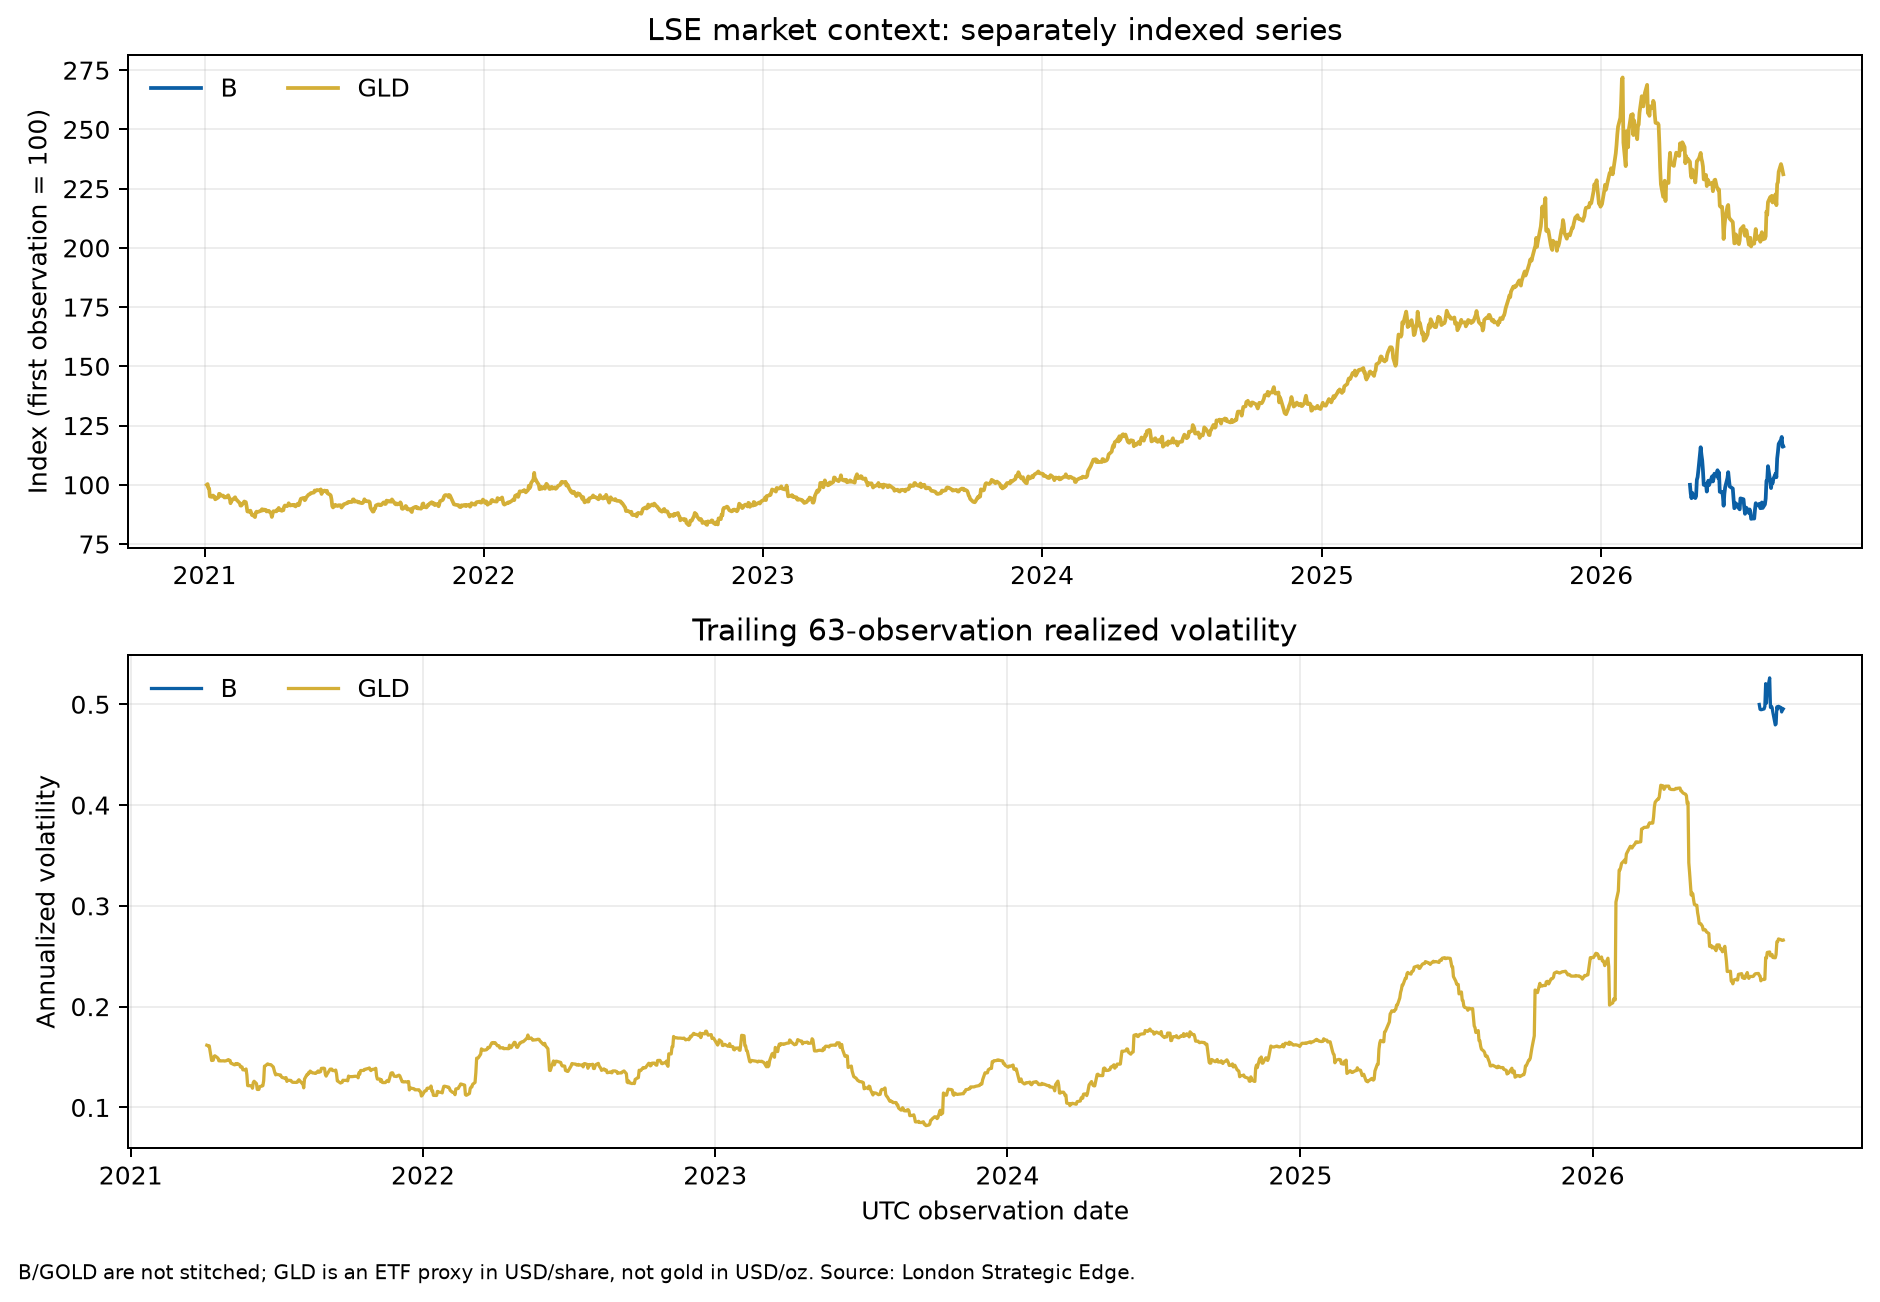
\includegraphics[width=0.98\textwidth]{img/lse/lse_market_context_20260826.png}
\caption{Separately indexed LSE series and trailing 63-observation realized
volatility. Barrick \texttt{B} is shown only over the catalog-valid interval;
GLD is an ETF proxy in USD/share. The discontinuous coverage is deliberate and
prevents an unsupported \texttt{GOLD}$\rightarrow$\texttt{B} stitch.}
\label{fig:lse-current-market-context}
\end{figure}


\part{Mathematical, Econometric and Numerical Foundations}
% AUTO-GENERATED by Github-Branch/tools/build_unified_source.ps1.
% Do not edit this file directly: update the transformation manifest instead.
\chapter{Measure, Probability and Stochastic Processes}
\chapterstatus{Edited reuse from Team 1. Mathematical and source-to-claim review remains open; figures are withheld pending the figure ledger.}
\sourceassetnote
\section{Measure theory and probability introduction}
\subsection{Measurable Spaces}

A measurable space is a pair consisting of a set and a $\sigma$-algebra.
A particularly important example is a Borel space, where the $\sigma$-algebra is the Borel $\sigma$-algebra of a topological space.

\par
A measurable space captures and generalises intuitive notions such as length, area, and volume with a set $X$ of ``points'' in the space. However, regions of the space are the elements of the $\sigma$-algebra, since intuitive measures are not usually defined for individual points. The algebra also captures relationships between regions: a region can be defined as an intersection of other regions, a union of other regions, or the space with the exception of another region.

\par
\textbf{Definition.} Consider a set $X$ and a $\sigma$-algebra $\mathcal{F}$ on $X$. Then the tuple $(X, \mathcal{F})$ is called a \textit{measurable space}. The elements of $\mathcal{F}$ are called \textit{measurable sets} within the measurable space.

\par
Note that, in contrast to a \textit{measure space}, no measure is needed for a measurable space.

\par
\textbf{Example.} Consider the set $X = \{1, 2, 3\}$. One possible $\sigma$-algebra would be 
\[
\mathcal{F}_1 = \{ X, \emptyset \}.
\]
Then $(X, \mathcal{F}_1)$ is a measurable space. Another possible $\sigma$-algebra is the power set of $X$:
\[
\mathcal{F}_2 = \mathcal{P}(X).
\]
With this, a second measurable space on the set $X$ is given by $(X, \mathcal{F}_2)$.

\par
\textbf{Common measurable spaces.}  
If $X$ is finite or countably infinite, the $\sigma$-algebra is most often the power set on $X$, so $\mathcal{F} = \mathcal{P}(X)$. This leads to the measurable space $(X, \mathcal{P}(X))$.

\par
If $X$ is a topological space, the $\sigma$-algebra is most commonly the \textit{Borel $\sigma$-algebra} $\mathcal{B}$, so $\mathcal{F} = \mathcal{B}(X)$. This leads to the measurable space $(X, \mathcal{B}(X))$, which is common for all topological spaces such as the real numbers $\mathbb{R}$.

\par
\textbf{Probability spaces.}  
A probability space is a measurable space equipped with a measure that is normalized. Formally, a probability space is a triple $(\Omega, \mathcal{F}, \mathbb{P})$, where $(\Omega, \mathcal{F})$ is a measurable space and $\mathbb{P} : \mathcal{F} \to [0,1]$ is a measure such that $\mathbb{P}(\Omega) = 1$. The set $\Omega$ is called the sample space, and elements of $\mathcal{F}$ are called events.
\subsection{Sigma-Algebras}

In mathematical analysis and probability theory, a \textbf{$\sigma$-algebra} (``sigma algebra'') is part of the formalism for defining sets that can be measured. In calculus and analysis, for example, $\sigma$-algebras are used to define the concept of sets with area or volume. In probability theory, they are used to define events with a well-defined probability. In this way, $\sigma$-algebras help to formalize the notion of size.

\par
In formal terms, a $\sigma$-algebra (also called a \textbf{$\sigma$-field}, where the $\sigma$ comes from the German word \textit{``Summe''}, meaning ``sum'') on a set $X$ is a nonempty collection $\Sigma \subseteq \mathcal{P}(X)$ of subsets of $X$ such that:
\begin{itemize}
    \item $X \in \Sigma$,
    \item if $A \in \Sigma$, then its complement $A^c := X \setminus A \in \Sigma$,
    \item if $(A_n)_{n \in \mathbb{N}} \subseteq \Sigma$, then $\bigcup_{n=1}^{\infty} A_n \in \Sigma$.
\end{itemize}
From these properties it follows that $\Sigma$ is also closed under countable intersections.

\par
The ordered pair $(X, \Sigma)$ is called a \textit{measurable space}.

\par
The set $X$ is understood to be an ambient space (such as the two-dimensional plane or the set of outcomes when rolling a six-sided dice, $\{1,2,3,4,5,6\}$), and the collection $\Sigma$ is a choice of subsets declared to have a well-defined size. The closure requirements for $\sigma$-algebras are designed to capture our intuitive ideas about how sizes combine.

\par
The definition of a $\sigma$-algebra resembles other mathematical structures such as a \textit{topology} or a \textit{set algebra}.
\paragraph{Examples of $\sigma$-Algebras}

If $X = \{ a, b, c, d \}$, one possible $\sigma$-algebra on $X$ is
\[
\Sigma = \{ \varnothing, \{a,b\}, \{c,d\}, \{a,b,c,d\} \}.
\]

\par
If $\{A_1, A_2, A_3, \ldots\}$ is a countable partition of $X$, then the collection of all unions of sets in the partition (including the empty set) is a $\sigma$-algebra.

\par
A more useful example is the set of subsets of the real line $\mathbb{R}$ formed by starting with all open intervals and closing under countable unions, countable intersections, and complements. This construction is known as the \textit{Borel $\sigma$-algebra}.
\subsection{Measure}

A \textit{measure} on $X$ is a function
\[
\mu : \mathcal{F} \to [0, +\infty]
\]
defined on a $\sigma$-algebra $\mathcal{F}$ such that:
\begin{itemize}
    \item $\mu(\emptyset) = 0$,
    \item (countable additivity) if $(A_n)_{n \in \mathbb{N}}$ are pairwise disjoint sets in $\mathcal{F}$, then
    \[
    \mu\left( \bigcup_{n=1}^{\infty} A_n \right) = \sum_{n=1}^{\infty} \mu(A_n).
    \]
\end{itemize}

\par
This formalizes the idea of assigning a consistent notion of ``size'' to sets.

\par
Ideally, one would like to assign a size to every subset of $X$, but in many natural settings this is not possible. For example, the \textit{axiom of choice} implies that there exist subsets of $\mathbb{R}$ (such as Vitali sets) that are not measurable.

\par
For this reason, one considers instead a smaller collection of privileged subsets of $X$, called the \textit{measurable sets}, which form a $\sigma$-algebra.

\section{Random variables, Lebesgue integrals and convergence theorems}
\subsection{Random variables}

A \textbf{random variable} $X$ is a measurable function
\[
X : \Omega \to E
\]
from a sample space $\Omega$ (the set of possible outcomes) to a measurable space $(E, \mathcal{E})$, where typically $E = \mathbb{R}$ or $\mathbb{R}^n$ equipped with the Borel $\sigma$-algebra.

\par
The technical, axiomatic definition requires the sample space $\Omega$ to belong to a \textit{probability triple} $(\Omega, \mathcal{F}, P)$, where $\mathcal{F}$ is a $\sigma$-algebra of events and $P$ is a probability measure.

\par
The measurability of $X$ means that for every measurable set $S \in \mathcal{E}$,
\[
X^{-1}(S) := \{ \omega \in \Omega \mid X(\omega) \in S \} \in \mathcal{F}.
\]

\par
The probability that $X$ takes on a value in a measurable set $S \subseteq E$ is therefore written as
\[
P(X \in S) = P(X^{-1}(S)).
\]
\subsection{Density function, expectation, variance}

A real-valued random variable $X$ is described by means of its cumulative distribution function (CDF),
\[
F_X(x) := \mathbb{P}[X \leq x].
\]

\par
If $X$ has an \textit{absolutely continuous} distribution, then it admits a probability density function (PDF) $f_X$ such that
\[
F_X(x) = \int_{-\infty}^{x} f_X(t)\,dt, \qquad \text{and} \qquad f_X(x) = \frac{dF_X(x)}{dx}.
\]
In general, not every random variable admits a density: discrete or mixed distributions do not have a PDF in this sense.

\par
The expected value of a random variable $X$ is defined in general (measure-theoretically) as the Lebesgue integral
\[
\mathbb{E}[X] = \int_{\Omega} X(\omega)\, dP(\omega),
\]
provided the integral $\int_{\Omega} |X|\, dP < \infty$.

\par
In the absolutely continuous case with density $f_X$, this reduces to
\[
\mathbb{E}[X] = \int_{-\infty}^{+\infty} x f_X(x)\, dx.
\]

\par
The variance of $X$, $\mathrm{Var}[X]$, is defined as
\[
\mathrm{Var}[X] = \int_{\Omega} (X - \mathbb{E}[X])^2\, dP,
\]
whenever the integral exists. In the case of a density,
\[
\mathrm{Var}[X] = \int_{-\infty}^{+\infty} (x - \mathbb{E}[X])^2 f_X(x)\, dx.
\]

\par
For a random variable $X$ and some constant $a \in \mathbb{R}$, the expectation of an indicator function is related to the CDF of $X$ as follows:
\[
\mathbb{E}[\mathbf{1}_{X \leq a}] = \int_{\Omega} \mathbf{1}_{\{X \leq a\}}\, dP = P(X \leq a) = F_X(a),
\]
where the indicator function of a set $A \in \mathcal{F}$ is defined by
\[
\mathbf{1}_A(\omega) = 
\begin{cases} 
1 & \omega \in A, \\
0 & \omega \notin A. 
\end{cases} \tag{1.1}
\]

\begin{definition}[Survival probability]
The survival probability is directly linked to the CDF. If $X$ is a random variable which denotes the lifetime, for example, in a population, then $\mathbb{P}[X \leq x]$ indicates the probability of not reaching the age $x$. The survival probability, defined by
\[
\mathbb{P}[X > x] = 1 - \mathbb{P}[X \leq x] = 1 - F_X(x),
\]
indicates the probability of surviving a lifetime of length $x$.
\end{definition}
\subsection{Lebesgue integral and convergence theorems}

The Lebesgue integral extends the classical Riemann integral by integrating with respect to a measure rather than over intervals. This allows integration of a wider class of functions and provides better convergence properties.

\par
One key difference is that the Lebesgue integral is defined by approximating functions via simple functions and measuring the size of their level sets, rather than partitioning the domain.

\par
The following convergence results are fundamental:

\begin{itemize}
    \item \textbf{Monotone Convergence Theorem (MCT):}  
    If $(X_n)$ is an increasing sequence of non-negative measurable functions, then
    \[
    \lim_{n \to \infty} \int X_n\, dP = \int \lim_{n \to \infty} X_n\, dP.
    \]

    \item \textbf{Fatou's Lemma:}  
    For a sequence $(X_n)$ of non-negative measurable functions,
    \[
    \int \liminf_{n \to \infty} X_n\, dP \leq \liminf_{n \to \infty} \int X_n\, dP.
    \]

    \item \textbf{Dominated Convergence Theorem (DCT):}  
    If $X_n \to X$ pointwise and $|X_n| \leq Y$ for some integrable function $Y$, then
    \[
    \lim_{n \to \infty} \int X_n\, dP = \int X\, dP.
    \]
\end{itemize}

\par
These results justify the interchange of limits and integrals under suitable conditions and are essential in probability theory and analysis.

\section{Filtration and Stochastic Processes}
\subsection{Stochastic processes and filtration}
We will often work with stochastic processes for the financial asset prices, and give some basic definitions for them here.
A \textbf{stochastic process}, $X(t)$, is a collection of random variables indexed by a time variable $t$.
Suppose we have a set of calendar dates/days, $T_1, T_2, \ldots, T_m$. Up to today, we have observed certain state values of the stochastic process $X(t)$. The past is known, and we therefore "see" the historical asset path. For the future we do not know the precise path but we may simulate the future according to some asset price distribution.

The mathematical tool which helps us describe the knowledge of a stochastic process up-to a certain time $T_i$ is the \textbf{sigma-field}, also known as \textbf{sigma-algebra}. The ordered sequence of sigma-fields is called a \textbf{filtration}, $\mathcal{F}(T_i) := \sigma(X(T_j) : 1 \leq j \leq i)$, generated by the sequence $X(T_j)$ for $1 \leq j \leq i$. The information available at time $T_i$ is thus described by a filtration. As we consider a sequence of observation dates, $T_1, \ldots, T_i$, we deal in fact with a sequence of filtrations, $\mathcal{F}(T_1) \subseteq \cdots \subseteq \mathcal{F}(T_i)$.

If we write that a process is $\mathcal{F}(T)$-measurable, we mean that at any time $t \leq T$, the realizations of this process are known. A simple example for this may be the market price of a stock and its historical values, i.e., we know the stock values up to today exactly, but we do not know any future values. We then say "the stock is today measurable". However, when we deal with an SDE model for the stock price, the value may be $T$ measurable, as we know the distribution for the period $T$ of a financial contract.

A stochastic process $X(t)$, $t \geq 0$, is said to be \textbf{adapted} to the filtration $\mathcal{F}(t)$, if
\[
\sigma(X(t)) \subseteq \mathcal{F}(t).
\]
By the term "adapted process" we mean that a stochastic process "cannot look into the future". In other words, for a stochastic process $X(t)$ its realizations (paths), $X(s)$ for $0 \leq s < t$, are known at time $s$ but not yet at time $t$.
\subsection{Martingales}

An important notion when dealing with stochastic processes is the martingale property.

\begin{definition}[Martingale]
Consider a probability space $(\Omega, \mathcal{F}, \mathbb{Q})$ equipped with a filtration $\{\mathcal{F}(t)\}_{t \ge 0}$.  
A right–continuous process $X(t)$ with left limits (a \emph{càdlàg} process) for $t \in [0,T]$ is said to be a martingale with respect to the filtration $\{\mathcal{F}(t)\}$ under the measure $\mathbb{Q}$ if, for all $s < t$, the following conditions hold:
\begin{align}
\mathbb{E}[\,|X(t)|\,] &< \infty, \\
\mathbb{E}[\,X(t)\mid \mathcal{F}(s)\,] &= X(s).
\end{align}
\end{definition}

The definition implies that the best prediction of a martingale’s future value is its present value. Indeed, for any $\Delta t > 0$,
\[
\mathbb{E}\big[X(t+\Delta t) - X(t)\mid \mathcal{F}(t)\big] = 0.
\]

\begin{remark}
A martingale represents a ``fair game'': once the current value $X(t)$ is known, the expected future change is zero. The process exhibits no predictable drift, and the conditional expectation of all future values equals the present value.
\end{remark}
\subsection{Adapted stochastic process}

We first need to introduce the binomial asset-pricing model in order to understand the following concepts.

\begin{definition}[Binomial asset pricing] 
In the \emph{binomial asset-pricing model}, time is divided into $N$ discrete steps.  
The price of a risky asset evolves according to
\[
S_{n+1} = 
\begin{cases}
u S_n, & \text{with probability } p,\\[4pt]
d S_n, & \text{with probability } 1-p,
\end{cases}
\]
where $u>1$ and $0<d<1$ are the up and down factors, respectively, and $S_0$ is the initial price.  
A risk-free asset grows deterministically at rate $r$, so its value satisfies
\[
B_{n+1} = (1+r) B_n.
\]
The model assumes $d < 1+r < u$ to exclude arbitrage.
\end{definition}

\begin{definition}
    Consider the binomial asset-pricing model and let
\[
M_0, M_1, \ldots, M_N
\]
be a sequence of random variables such that each $M_n$ depends only on the first $n$ coin tosses (with $M_0$ constant).  
Such a sequence is called an \emph{adapted stochastic process}.
\begin{enumerate}
    \item If for every $n = 0, 1, \ldots, N-1$,
    \[
    M_n = \mathbb{E}_n[M_{n+1}],
    \]
    we say that the process is a \emph{martingale}.

    \item If
    \[
    M_n \le \mathbb{E}_n[M_{n+1}], \qquad n = 0,1,\ldots,N-1,
    \]
    we say that the process is a \emph{submartingale}.

    \item If
    \[
    M_n \ge \mathbb{E}_n[M_{n+1}], \qquad n = 0,1,\ldots,N-1,
    \]
    we say that the process is a \emph{supermartingale}.
\end{enumerate}
\end{definition}

\textbf{Remark}  
The martingale property above is stated as a one-step-ahead condition,  
but it automatically implies an analogous condition for any number of steps.  
If $M_0, M_1, \ldots, M_N$ is a martingale and $n \le N-2$, then
\[
M_{n+1} = \mathbb{E}_{n+1}[M_{n+2}].
\]
Taking conditional expectations with respect to the information at time $n$, and using the tower property of conditional expectation, we obtain
\[
\mathbb{E}_n[M_{n+1}]
= \mathbb{E}_n\!\left( \mathbb{E}_{n+1}[M_{n+2}] \right)
= \mathbb{E}_n[M_{n+2}].
\]
Because $\mathbb{E}_n[M_{n+1}] = M_n$, this yields the “two-step-ahead’’ relation
\[
M_n = \mathbb{E}_n[M_{n+2}].
\]
Iterating the argument, for any $0 \le n \le m \le N$ we obtain the general multistep property:
\[
M_n = \mathbb{E}_n[M_m].
\]

\medskip

\textbf{Remark}  
A martingale has constant expectation over time.  
If $M_0, M_1, \ldots, M_N$ is a martingale, then
\[
M_0 = \mathbb{E}[M_n], \qquad n = 0,1,\ldots,N.
\]
Indeed, taking expectations on both sides of the martingale relation
\[
M_n = \mathbb{E}_n[M_{n+1}],
\]
and using the tower property, we find that $\mathbb{E}[M_n] = \mathbb{E}[M_{n+1}]$ for all $n$.  
Since $M_0$ is deterministic, $M_0 = \mathbb{E}[M_0]$, and the conclusion follows.
\subsection{Markov process}


\begin{definition}[Markov process] Consider the binomial asset-pricing model.  
Let $X_0, X_1, \ldots, X_N$ be an adapted process.  
If, for every $n$ between $0$ and $N-1$ and for every function $f(x)$,  
there exists another function $g(x)$ (depending on $n$ and $f$) such that
\begin{equation}
    \mathbb{E}_n[f(X_{n+1})] = g(X_n),
\end{equation}
we say that $X_0, X_1, \ldots, X_N$ is a Markov process.
\end{definition}

\begin{remark}
The Markov property expresses the idea that the process has no memory beyond its current state. Once $X_n$ is known, the conditional distribution of $X_{n+1}$ does not depend on the earlier values $X_0,\ldots,X_{n-1}$. Thus, the present state contains all the information necessary for predicting the next step.
\end{remark}


By definition, $\mathbb{E}_n[f(X_{n+1})]$ is a random quantity, since it depends on the first $n$ coin tosses. The Markov property states that this dependence occurs entirely through $X_n$; that is, all the information from the coin-toss history that is needed to evaluate $\mathbb{E}_n[f(X_{n+1})]$ is summarized by $X_n$.

At this stage, we are not focused on deriving an explicit formula for the function $g$, but rather on emphasizing its existence. The mere existence of such a function implies that if the payoff of a derivative security is random only through its dependence on $X_N$, then there is a version of the pricing algorithm that does not require storing the entire path of the process.

The martingale property arises as a particular instance of ${E}_n[f(X_{n+1})] = g(X_n)$ when  $f(x) = x$ and $g(x) = x$. For a process to qualify as Markov, it must satisfy ${E}_n[f(X_{n+1})] = g(X_n)$ for \emph{every} function $f$, with some corresponding function $g$.
Thus, while every martingale satisfies this relation for the specific choice $f(x) = x$, this alone does not ensure that the process is Markov. In fact, a general martingale need not be Markov.

Conversely, even when we restrict attention to the function $f(x) = x$, the Markov property merely requires that 
\[
\mathbb{E}_n[M_{n+1}] = g(M_n)
\]
for some function $g$; it does not insist that $g(x) = x$. Therefore, a Markov process is not necessarily a martingale.

\begin{definition}[Transition probabilities]
A Markov process $\{X_n\}$ is characterized by the transition probabilities
\[
P_n(x,A) := \mathbb{P}(X_{n+1} \in A \mid X_n = x),
\]
where $A$ is any measurable subset of the state space. For any function $f$, the function $g$ appearing in
\[
\mathbb{E}_n[f(X_{n+1})] = g(X_n)
\]
is given by the integral representation
\[
g(x) = \int f(y)\, P_n(x)dy.
\]
\end{definition}


The next lemma frequently provides a crucial step in confirming that a
given process possesses the Markov property.

\textbf{Lemma (Independence).}
In the $N$-period binomial asset–pricing model, let $n$ be an integer with $0 \leq n \leq N$. Suppose the random variables
\[
X_1,\ldots,X_K
\]
depend only on coin tosses $1$ through $n$, and the random variables
\[
Y_1,\ldots,Y_L
\]
depend only on coin tosses $n+1$ through $N$.  
(The superscripts $1,\ldots,K$ on $X$ and $1,\ldots,L$ on $Y$ are indices, not exponents.)

Let 
\[
f(x_1,\ldots,x_K,y_1,\ldots,y_L)
\]
be a function of dummy variables, and define the random variable
\begin{equation}
Z := f(X_1,\ldots,X_K,\,Y_1,\ldots,Y_L).
\end{equation}

Because the $X$'s depend only on the first $n$ coin tosses and the $Y$'s only on the remaining ones, the $X$'s are independent of the $Y$'s conditional on the information available at time $n$. Hence the conditional expectation satisfies
\begin{equation}
\mathbb{E}_n[Z]
  = \mathbb{E}_n\!\left[ f(X_1,\ldots,X_K,Y_1,\ldots,Y_L) \right]
  = g(X_1,\ldots,X_K),
\end{equation}
where the function $g$ is given by
\[
g(x_1,\ldots,x_K)
   := \mathbb{E}\!\left[ f(x_1,\ldots,x_K,Y_1,\ldots,Y_L) \right].
\]

Thus the conditional expectation with respect to $\mathcal{F}_n$ averages only over the randomness in $Y_1,\ldots,Y_L$, treating the $X$'s as fixed.

\section{Brownian Motion}
\subsection{Introduction}
The concept of \textit{Brownian motion} takes its origins in physics to describe the random movement of a particle suspended in a fluid. The mathematical formalization of this phenomenon, introduced by Wiener in the early 20th century, gave rise to one of the cornerstones of probability theory: the \textit{Wiener process} or \textit{standard Brownian motion}.

Brownian motion finds its particular significance in finance, where it serves as the paradigm of randomness in price movements.
\subsection{Definition and Fundamental Properties}

We first begin with the definition of standard Brownian motion. A stochastic process \( \{W_t\}_{t \geq 0} \) defined on a probability space \( (\Omega, \mathcal{F}, \mathbb{P}) \) is called a \textbf{standard Brownian motion} if it satisfies the following properties:
\begin{enumerate}
    \item \( W_0 = 0 \) almost surely;
    \[
    \mathcal{P}[W_U = 0] = 1.
    \]
    \item For every \( 0 \leq s < t \), the increment \( W_t - W_s \) is normally distributed with mean zero and variance \( t - s \), that is,
    \[
    W_t - W_s \sim \mathcal{N}(0, t-s);
    \]
    \item The increments are independent, meaning that for any sequence of times \( 0 \leq t_0 < t_1 < \cdots < t_n \),
    \[
    W_{t_1} - W_{t_0}, \, W_{t_2} - W_{t_1}, \, \ldots, \, W_{t_n} - W_{t_{n-1}}
    \quad \text{are independent};
    \]
    \item The sample paths of \( W_t \) are almost surely continuous.
\end{enumerate}


These properties uniquely characterize standard Brownian motion. The combination of Gaussian independent increments and continuity makes it a central process in modeling continuous random phenomena.
\subsection{Construction of Brownian Motion}
Up to this point, we have described the main properties that a Brownian motion should satisfy. 
However, stating its properties is not enough to guarantee that a process with such characteristics actually exists.
Hence, we need to prove the existence of such a process.
From a theoretical standpoint, the Brownian motion can be constructed in several ways, two classical and fundamental approaches are:

\begin{enumerate}
    \item \textbf{Kolmogorov's Construction}

    We begin by fixing a finite set of times $0 \le t_1 < t_2 < \dots < t_n$ and defining the joint distribution of the random vector
\[
(W_{t_1}, W_{t_2}, \dots, W_{t_n}).
\]
We require this vector to be multivariate normal with mean zero and covariance matrix
\[
\text{Cov}(W_{t_i}, W_{t_j}) = \min(t_i, t_j), \quad 1 \le i,j \le n.
\]
The intuition behind this covariance choice is as follows. For $s < t$, we can write
\[
W_t = W_s + (W_t - W_s).
\]
By definition of Brownian motion, the increment $(W_t - W_s)$ is independent of the past (including $W_s$) and has variance $t-s$. 
Therefore, the covariance satisfies
\[
\text{Cov}(W_s, W_t) = \text{Cov}(W_s, W_s + (W_t - W_s)) = \text{Var}(W_s) = s = \min(s,t),
\]
because the increment does not contribute to the covariance. 
In other words, the covariance function $\min(s,t)$ encodes two key properties at once: the independence of increments and the linear growth of variance with time.
    
    
Next, we must ensure that these finite-dimensional distributions are compatible with each other, a property called \emph{consistency}. 

A family of finite-dimensional distributions $\{\mu_{t_1, \dots, t_n}\}$ is \emph{consistent} if, for any subset of times, the marginal distribution of $\mu_{t_1, \dots, t_n}$ corresponding to the subset coincides with the distribution defined directly for those times. 
Intuitively, consistency ensures that all “pieces” of the process fit together.

Kolmogorov's Extension Theorem then guarantees the existence of a stochastic process with the given finite-dimensional distributions.

\begin{theorem}[Kolmogorov's Extension Theorem]
Let $\{\mu_{t_1, \dots, t_n}\}$ be a consistent family of finite-dimensional distributions indexed by finite ordered subsets of $[0, \infty)$. 
Then, there exists a probability space $(\Omega, \mathcal{F}, \mathbb{P})$ and a stochastic process $\{X_t\}_{t \ge 0}$ such that, for any $t_1 < \dots < t_n$, the joint distribution of $(X_{t_1}, \dots, X_{t_n})$ coincides with $\mu_{t_1, \dots, t_n}$.
\end{theorem}    


In our case, the Gaussian distributions defined above are consistent because taking the marginal of a multivariate normal distribution yields another multivariate normal with the correct mean and covariance. 
Hence, Kolmogorov's theorem ensures the existence of a stochastic process $(W_t)_{t \ge 0}$ with the desired finite-dimensional distributions.

While existence is guaranteed, continuity of sample paths is not. To obtain continuity, we use the \textit{Kolmogorov–Chentsov Continuity Theorem}.

\begin{theorem}[Kolmogorov–Chentsov Continuity Theorem]
Let $\{X_t\}_{t \ge 0}$ be a stochastic process. 
If there exist constants $\alpha, \beta, C > 0$ such that
\[
\mathbb{E}[|X_t - X_s|^{\alpha}] \le C |t-s|^{1+\beta}, \quad \forall s,t \ge 0,
\]
then there exists a \emph{modification} of $X_t$ with continuous sample paths almost surely.
\end{theorem}

For Brownian motion, the fourth moment of the increments satisfies
\[
\mathbb{E}[(W_t - W_s)^4] = 3 (t - s)^2,
\]
which fits the theorem with $\alpha = 4$ and $\beta = 1$. 
Therefore, a continuous version of the process exists.

In conclusion, we have constructed a stochastic process $(W_t)_{t \ge 0}$ that satisfies:

\begin{itemize}
    \item $W_0 = 0$ almost surely;
    \item independent Gaussian increments with variance equal to the length of the interval;
    \item covariance function $\text{Cov}(W_s, W_t) = \min(s,t)$, encoding both independence of increments and linear variance growth;
    \item continuous sample paths almost surely.
\end{itemize}

    
    \item \textbf{The Random Walk Limit}
    
Another method used to create the classic Brownian Motion is the Random Walk Limit. This method provides an intuitive link between discrete-time models and the continuous-time stochastic dynamics used in finance. It considers a sequence of independent and identically distributed (i.i.d.) random variables $\{\xi_i\}_{i \in \mathbb{N}}$, with zero mean ($E[\xi_i] = 0$) and unit variance ($\text{Var}(\xi_i) = 1$). The rescaled random walk process $\{W^{(n)}_t\}_{t \geq 0}$ is defined as:
    
    $$
    W^{(n)}_t = \frac{1}{\sqrt{n}} \sum_{i=1}^{\lfloor nt \rfloor} \xi_i
    $$
    
where $\lfloor nt \rfloor$ denotes the integer part of $nt$, corresponding to the number of steps up to time $t$.

The scaling factor $\frac{1}{\sqrt{n}}$ is crucial: it ensures that, as the number of steps $n$ increases, the variance of $W^{(n)}_t$ grows linearly with time, matching the defining property of Brownian motion. 

As $n \to \infty$, the process $W^{(n)}_t$ converges in distribution to a continuous-time process $\{W_t\}_{t \ge 0}$, which is the standard Brownian motion. 

Intuitively, as the time steps become finer and the step sizes are appropriately scaled, the discrete jumps of the random walk become infinitesimally small and occur infinitely often in a finite interval. In the limit, the random walk “smooths out” into a continuous, nowhere-differentiable path. The key features of Brownian motion: zero mean, independent increments, variance proportional to elapsed time and continuity of paths emerge naturally from this limiting procedure. 
\end{enumerate}

% Asset/code block omitted pending provenance acceptance.
\subsection{Basic Properties of Brownian Motion}

Based on the definition provided in the previous section, the standard Brownian motion $\{W_t\}_{t \ge 0}$ possesses several fundamental properties that are crucial for its application in stochastic calculus and financial modeling.
\paragraph{Expected Value and Covariance}
The Gaussian nature and the property of zero initial state ($W_0=0$) lead directly to the mean and covariance functions:

\begin{enumerate}
    \item \textbf{Expected Value (Mean):} The expected value of Brownian motion at any time $t$ is zero.
    \[
    \mathbb{E}[W_t] = 0, \quad \forall t \ge 0.
    \]
    This follows from the fact that $W_t = (W_t - W_0)$ is normally distributed as $\mathcal{N}(0, t)$, which has a mean of zero.

    \item \textbf{Variance:} The variance of Brownian motion is linear in time.
    \[
    \text{Var}(W_t) = \mathbb{E}[W_t^2] = t, \quad \forall t \ge 0.
    \]

    \item \textbf{Covariance Function:} For any $s, t \ge 0$, the covariance between $W_s$ and $W_t$ is given by the minimum of the two times:
    \[
    \text{Cov}(W_s, W_t) = \min(s, t).
    \]
    If we assume, without loss of generality, that $s \le t$, we can derive this property as follows, leveraging the independence of increments:
    \begin{align*}
    \text{Cov}(W_s, W_t) &= \text{Cov}(W_s, W_s + (W_t - W_s)) \\
    &= \text{Cov}(W_s, W_s) + \text{Cov}(W_s, W_t - W_s) \\
    &= \text{Var}(W_s) + 0 \\
    &= s = \min(s, t).
    \end{align*}
\end{enumerate}

% Asset/code block omitted pending provenance acceptance.
\paragraph{Martingale Property}
The independence of future increments from the past information is the key feature that establishes the Brownian motion as a martingale.


For standard Brownian motion $\{W_t\}_{t \ge 0}$ and its natural filtration $\{\mathcal{F}_t\}$, we have:
\begin{align*}
\mathbb{E}[W_t | \mathcal{F}_s] &= \mathbb{E}[W_s + (W_t - W_s) | \mathcal{F}_s] \\
&= \mathbb{E}[W_s | \mathcal{F}_s] + \mathbb{E}[W_t - W_s | \mathcal{F}_s] \\
&= W_s + \mathbb{E}[W_t - W_s] \\
&= W_s + 0 = W_s.
\end{align*}
The steps rely on the facts that $W_s$ is $\mathcal{F}_s$-measurable, and the increment $(W_t - W_s)$ is independent of $\mathcal{F}_s$ and has zero mean. Thus, $\mathbf{W_t}$ is a martingale.
\paragraph{Markov Property}
Brownian motion is also a Markov Process. 
For Brownian motion, $W_t$ can be written as $W_t = W_s + (W_t - W_s)$. Since the future increment $(W_t - W_s)$ is independent of the past $\{\mathcal{F}_s\}$ and $W_s$ summarizes all the necessary history for the transition, the future movement starting at $W_s$ is independent of how $W_s$ was reached. This makes $\mathbf{W_t}$ a Markov process.
\paragraph{Exponential Transformation and Martingale (Girsanov's Theorem)}
A particularly important transformation in mathematical finance is the exponential of the Brownian motion, especially the process known as the exponential martingale or Doléans-Dade exponential, which appears in the context of the Girsanov Theorem.

The process $Z_t$ defined by:
\[
Z_t = \exp \left( \alpha W_t - \frac{1}{2} \alpha^2 t \right)
\]
is a martingale for any real constant $\alpha$. This process, often called the Novikov Martingale (or simply the exponential martingale), is a key component in changing the probability measure (change of measure). The term $-\frac{1}{2}\alpha^2 t$ acts as a compensator to ensure that $\mathbb{E}[Z_t] = 1$, which is a necessary condition for a non-negative martingale with $Z_0=1$.

We confirm the martingale property using the expectation $\mathbb{E}[Z_t | \mathcal{F}_s] = Z_s$:
\[
\mathbb{E}[Z_t | \mathcal{F}_s] = Z_s \quad \text{almost surely}.
\]
This property will be fundamental later in deriving the risk-neutral measure in the Black-Scholes model.
\subsection{Filtration for Brownian Motion}

When applied to Brownian motion $\{W_t\}_{t \ge 0}$, the filtration $\{\mathcal{F}_t\}_{t \ge 0}$ represents the increasing collection of information generated by the process up to time $t$. This filtration must satisfy the following key properties reflecting the nature of Brownian motion:

\begin{enumerate}
    \item \textbf{Information accumulation:} For all $0 \le s < t$, the sigma-algebra $\mathcal{F}_s$ is contained in $\mathcal{F}_t$, meaning that information available at an earlier time is also available at later times.
    
    \item \textbf{Adaptedness:} The Brownian motion is adapted to $\{\mathcal{F}_t\}$, i.e., for each $t \ge 0$, the random variable $W_t$ is measurable with respect to $\mathcal{F}_t$. Thus, the value of $W_t$ is completely determined by the information known up to time $t$.
    
    \item \textbf{Independence of future increments:} For any $0 \le t < u$, the increment $W_u - W_t$ is independent of the sigma-algebra $\mathcal{F}_t$. This expresses the fundamental property that the future evolution of the Brownian motion cannot be predicted from past information.
\end{enumerate}

These properties formalize the intuitive understanding that Brownian motion “reveals” information progressively and that its future increments behave like fresh randomness independent of the past. This independence underlies many important theoretical results and practical models, including the efficient market hypothesis in financial mathematics, where past information cannot be used to forecast future price changes modeled by Brownian motion.

Moreover, any stochastic process $\{\Delta_t\}_{t \ge 0}$ is said to be adapted to the filtration $\{\mathcal{F}_t\}$ if, for every $t$, $\Delta_t$ is measurable with respect to $\mathcal{F}_t$. This ensures that $\Delta_t$ depends only on information available up to time $t$, a crucial requirement in stochastic calculus and modeling.
\section{SDEs and Geometric Brownian Motion}
In the world of finacial markets, asset's prices reflect both the present value of the firm and expectations about their future performance. These expectations, however, fluctuate over time introducing an uncertainty component into the asset price. The resulting randomness in asset prices is possible to model through the use of stochastic differential equations (SDEs).
SDEs provide analytical tools for validating numerical schemes and serve as building blocks for more sophisticated stochastic models of market dynamics.
Among all continuous-time models, the most fundamental is the Geometric Brownian Motion (GBM). In this framework, the logarithm of the asset price follows an arithmetic Brownian motion driven by a Wiener process. This ensures properties that align well with real-world financial data: prices remain strictly positive, returns are continuous and volatility acts proportionally to the current price level.
However, formulating and analysing the GBM model rigorously requires the mathematical machinery of stochastic calculus. Before introducing GBM explicitly, we therefore present the notions of stochastic integrands and square-integrable processes, develop the Itô integral, and establish the general theory of SDEs.
\subsection{Stochastic Integrands and SDEs}
The Stochastic Differential Equation (SDE) is defined in terms of the Itô integral with respect to the standard Brownian motion $W_t$. To ensure the existence and properties of this integral, the functions we integrate (the integrands) must satisfy specific mathematical conditions.
\paragraph{Stochastic Integrands and Square-Integrable Variables}
The Itô integral, $\int_0^T \Phi_t dW_t$, is constructed as a limit of sums (analogous to the Riemann sum) built on the properties of martingales and $L^2$ theory. The class of processes that can be integrated with respect to $W_t$ is restricted to ensure convergence in the mean-square sense.

\begin{definition}[Admissible Integrand]
A stochastic process $\Phi = \{\Phi_t\}_{t \geq 0}$ defined on the probability space $(\Omega, \mathcal{F}, \mathbb{P})$ is classified as an admissible integrand (or belonging to the space $\mathcal{L}^2(0, T)$) if it satisfies the following two conditions:
\begin{enumerate}
    \item Adaptedness: $\Phi_t$ is $\mathcal{F}_t$-adapted, meaning $\Phi_t$ depends only on the information available up to time $t$.
    \item Square-Integrability: $\Phi_t$ is square-integrable over the time interval $[0, T]$, i.e.,
    \[
    \mathbb{E} \left[ \int_0^T \Phi_t^2 dt \right] < \infty, \quad \text{for all } T > 0.
    \]
\end{enumerate}
\end{definition}
The condition of square-integrability for the process ensures that the variance of the resulting Itô integral, $\text{Var}\left( \int_0^T \Phi_t dW_t \right) = \mathbb{E} \left[ \int_0^T \Phi_t^2 dt \right]$, remains finite. Similarly, a random variable $X$ is square-integrable if its second moment is finite: $\mathbb{E}[X^2] < \infty$.
\paragraph{Stochastic Differential Equations (SDEs)}
A Stochastic Differential Equation describes a continuous-time process whose evolution is partially deterministic and partially stochastic, driven by Brownian motion.

\begin{definition}[General SDE]
A general form of a one-dimensional Stochastic Differential Equation is an equation for the stochastic process $\{X_t\}_{t \ge 0}$ written as:
\[
dX_t = \mu(t, X_t) dt + \sigma(t, X_t) dW_t, \quad X_0 = x_0,
\]
which is interpreted in its integral form:
\[
X_t = x_0 + \int_0^t \mu(u, X_u) du + \int_0^t \sigma(u, X_u) dW_u.
\]
\end{definition}
Here:
\begin{itemize}
    \item $X_t$ is the unknown stochastic process, often modeling an asset price or interest rate.
    \item $\mu(t, X_t)$ is the drift coefficient (or function), representing the deterministic component of the change, related to the expected growth.
    \item $\sigma(t, X_t)$ is the diffusion coefficient (or function), representing the intensity of the noise component, proportional to the volatility.
    \item The first integral is a standard Lebesgue integral, while the second is the Itô stochastic integral, which requires the integrand $\sigma(u, X_u)$ to be admissible.
\end{itemize}
Existence and uniqueness of the solution $X_t$ are typically guaranteed if the coefficients $\mu$ and $\sigma$ satisfy the local Lipschitz and linear growth conditions.
\subsection{Itô’s Formula}

In standard differential calculus, the chain rule is used to find the differential of a composite function, $Y_t = f(t, X_t)$, where $X_t$ is a deterministic differentiable function. However, the standard chain rule does not apply when $X_t$ is an Itô process.

The failure of the classical chain rule in the stochastic setting is fundamentally due to the \textbf{non-zero quadratic variation} of Brownian motion. For a smooth deterministic function, $(dx)^2 \approx 0$ as $dt \to 0$. However, for Brownian motion $W_t$, the differential $(dW_t)^2$ is of order $dt$ (formally, $E[(dW_t)^2] = dt$). When performing a Taylor expansion of $f(t, X_t)$, the second-order term $(dX_t)^2$ does not vanish in the limit, but instead contributes a first-order term to the differential. This "extra term" is known as the Itô term or the drift correction.
\paragraph{Construction via Summation}
The Itô formula can be heuristically derived by considering a partition of the time interval $[0, T]$, where $0 = t_0 < t_1 < \dots < t_n = T$. Let $\Delta X_j = X_{t_{j+1}} - X_{t_j}$. Using a Taylor expansion:
\[
f(T, X_T) - f(0, X_0) = \sum_{j=0}^{n-1} [f(t_{j+1}, X_{t_{j+1}}) - f(t_j, X_{t_j})]
\]
Expanding the terms inside the sum:
\[
\Delta f \approx \sum \frac{\partial f}{\partial t} \Delta t_j + \sum \frac{\partial f}{\partial x} \Delta X_j + \frac{1}{2} \sum \frac{\partial^2 f}{\partial x^2} (\Delta X_j)^2 + \dots
\]
As the mesh size of the partition goes to zero, the term $\sum (\Delta X_j)^2$ converges in probability to the quadratic variation $\langle X \rangle_T$. This summation process highlights that the Itô integral is defined by evaluating the integrand at the \textbf{left endpoint} of each sub-interval, i.e., $f(t_j, X_{t_j})$.

\begin{theorem}[Itô’s Formula]
Let $X_t$ be an Itô process defined by: $dX_t = \mu_t dt + \sigma_t dW_t$.
For $f \in C^{1,2}([0, \infty) \times \mathbb{R})$, the differential $dY_t$ of $Y_t = f(t, X_t)$ is:
\[
dY_t = \left( \frac{\partial f}{\partial t} + \frac{\partial f}{\partial x} \mu_t + \frac{1}{2} \frac{\partial^2 f}{\partial x^2} \sigma_t^2 \right) dt + \frac{\partial f}{\partial x} \sigma_t dW_t.
\]
\end{theorem}
\paragraph{Comparison: Itô vs. Stratonovich}
The choice of the evaluation point in the Riemann-sum construction leads to different stochastic integrals:

\begin{itemize}
    \item \textbf{Itô Integral ($\int X_t dW_t$):} Evaluates the integrand at the \textbf{left endpoint} ($t_j$). It is a martingale (under certain conditions) and is "non-anticipating," making it ideal for finance as it respects causality (information available at time $t$). However, it does not follow classical calculus rules.
    \item \textbf{Stratonovich Integral ($\int X_t \circ dW_t$):} Evaluates the integrand at the \textbf{midpoint} ($ \frac{t_j + t_{j+1}}{2} $).
     It \textbf{satisfies the classical chain rule} (the second-order term disappears in its formulation). However, it is not generally a martingale and "looks into the future" within each small interval, making it less intuitive for modeling financial price processes.
    
\end{itemize}
\subsection{Geometric Brownian Motion}

We now apply the general theory of stochastic integrals and Itô calculus to derive and analyse the most fundamental model for asset prices in continuous time: the \emph{Geometric Brownian Motion} (GBM). This model captures proportional growth, multiplicative noise and strict positivity of prices, and forms the basis of the Black--Scholes option pricing framework.
\paragraph{Definition of the GBM SDE}

\begin{definition}[Geometric Brownian Motion]
A stochastic process $S = \{S_t\}_{t \ge 0}$ is said to follow a \emph{Geometric Brownian Motion} if it satisfies the Stochastic Differential Equation
\begin{equation}
dS_t = \mu S_t\, dt + \sigma S_t\, dW_t, \qquad S_0 > 0,
\end{equation}
where
\begin{itemize}
    \item $\mu \in \mathbb{R}$ is the \emph{drift}, representing the expected rate of return,
    \item $\sigma > 0$ is the \emph{volatility}, representing the intensity of stochastic fluctuations,
    \item $W_t$ is a standard Brownian motion on the filtered probability space.
\end{itemize}
\end{definition}

The coefficients of the SDE,
\[
b(t,s) = \mu s, \qquad a(t,s) = \sigma s,
\]
are globally Lipschitz and satisfy linear growth conditions. Thus, by the fundamental existence and uniqueness theorem for SDEs, equation \sourceref{eq:GBM-SDE} has a unique strong solution.
\paragraph{Logarithmic Dynamics via Itô's Formula}

A key observation is that the logarithm of $S_t$ evolves as an arithmetic Brownian motion.  
Let $Y_t = \ln(S_t)$. Applying Itô’s formula to the function $f(s) = \ln s$ yields
\[
df(S_t)
= \frac{1}{S_t} dS_t 
- \frac12 \frac{1}{S_t^2} (dS_t)^2.
\]
Since $(dS_t)^2 = \sigma^2 S_t^2 dt$, substituting the SDE \sourceref{eq:GBM-SDE} gives
\begin{equation}
dY_t = \left( \mu - \tfrac{1}{2}\sigma^2 \right) dt + \sigma\, dW_t.
\end{equation}
Thus the logarithmic price process follows a linear SDE with constant coefficients.
\paragraph{Explicit Solution and Log-Normality}

Integrating \sourceref{eq:logS-dynamics} from $0$ to $t$ yields
\[
\ln(S_t)
= \ln(S_0)
+ \left(\mu - \tfrac{1}{2}\sigma^2\right)t
+ \sigma W_t.
\]
Exponentiating gives the explicit closed-form solution:
\begin{equation}
S_t
= S_0 \exp\!\left[
     \left(\mu - \tfrac12\sigma^2\right)t
     + \sigma W_t
   \right].
\end{equation}

From this expression we obtain several fundamental properties:

\begin{enumerate}
    \item \textbf{Strict positivity}:
    \[
    S_t > 0 \quad \text{a.s. for all } t \ge 0.
    \]

    \item \textbf{Log-normal distribution}:  
    Since $W_t \sim \mathcal{N}(0,t)$, it follows that
    \[
    \ln(S_t)
    \sim \mathcal{N}\!\left(
        \ln(S_0) + \left(\mu - \tfrac12 \sigma^2\right)t,
        \; \sigma^2 t
    \right).
    \]

    \item \textbf{Moments}:
    \[
    \mathbb{E}[S_t] = S_0 e^{\mu t}, \qquad
    \mathrm{Var}(S_t) = S_0^2 e^{2\mu t} \big( e^{\sigma^2 t} - 1 \big).
    \]
\end{enumerate}


% Asset/code block omitted pending provenance acceptance.
\paragraph{Interpretation in Financial Modelling}

The GBM SDE captures two essential facts commonly observed in financial markets, making it a natural starting point for modelling asset prices in continuous time.

\begin{itemize}
    \item \textbf{Proportional volatility:}  
    The diffusion term $\sigma S_t dW_t$ is proportional to the current level of the asset price. This implies that the magnitude of random fluctuations increases with the price itself. As a consequence, the model assumes that returns, rather than absolute price changes, exhibit a constant level of volatility over time. This property is consistent with empirical observations in financial data, where percentage changes tend to be more stable than absolute variations.

    \item \textbf{Strict positivity of prices:}  
    The explicit solution of the GBM, given in \sourceref{eq:GBM-solution}, is expressed as an exponential function of a Brownian motion. Since the exponential function is always strictly positive, it follows that $S_t > 0$ almost surely for all $t \ge 0$. This property is particularly important in financial modelling, as it ensures that asset prices cannot become negative.
\end{itemize}

\section{Risk-Neutral Pricing}
\subsection{Asset Prices Under the Physical Measure}

Throughout this chapter we assume that the asset price process satisfies
\[
\mathbb{E}[\,|S(t)|\,] < \infty,
\]
so that expectations of payoffs are well defined.

Under the real-world probability measure $\mathbb{P}$, the dynamics of a stock price are typically modelled by a geometric Brownian motion
\[
dS(t) = \mu S(t)\,dt + \sigma S(t)\, dW^{\mathbb{P}}(t),
\]
where $\mu$ denotes the expected rate of return and $\sigma>0$ the volatility.

The explicit solution of this stochastic differential equation is
\[
S(t) = S(t_0)\exp\left[\left(\mu-\frac{1}{2}\sigma^2\right)(t-t_0) + \sigma\big(W^{\mathbb P}(t)-W^{\mathbb P}(t_0)\big)\right].
\]

Taking conditional expectations yields
\[
\mathbb{E}_{\mathbb{P}}\!\left[ S(t)\mid \mathcal{F}_{t_0} \right]
= S(t_0)e^{\mu(t-t_0)}.
\]

Hence, over a short interval $\Delta t$,
\[
\mathbb{E}_{\mathbb{P}}\!\left[ S(t+\Delta t)\mid \mathcal{F}_t \right]
= S(t)e^{\mu\Delta t}.
\]

Since typically $\mu \neq r$, the discounted price process
\[
\tilde S(t)=e^{-rt}S(t)
\]
satisfies
\[
d\tilde S(t)
=
(\mu-r)\tilde S(t)dt
+
\sigma\tilde S(t)dW^{\mathbb P}(t),
\]
and therefore it is generally \emph{not} a martingale under the physical measure $\mathbb{P}$.
\subsection{Risk-Neutral Measure and Discounted Martingales}

A central idea of modern asset pricing theory is to introduce an alternative probability measure $\mathbb{Q}$, called the \emph{risk-neutral measure}, under which discounted asset prices become martingales.

\par
The passage from $\mathbb{P}$ to $\mathbb{Q}$ is achieved via a change of measure. Define the process
\[
\lambda := \frac{\mu - r}{\sigma},
\]
called the \textit{market price of risk}. Then, by \textit{Girsanov's theorem}, there exists a probability measure $\mathbb{Q}$ equivalent to $\mathbb{P}$ such that the process
\[
W^{\mathbb{Q}}(t) := W^{\mathbb{P}}(t) + \lambda t
\]
is a Brownian motion under $\mathbb{Q}$.

\par
Equivalently, the change of measure can be expressed via the Radon--Nikodym derivative
\[
\frac{d\mathbb{Q}}{d\mathbb{P}}\Big|_{\mathcal{F}_t}
=
\exp\left(
- \lambda W^{\mathbb{P}}(t)
- \frac{1}{2}\lambda^2 t
\right).
\]

\par
Under $\mathbb{Q}$ the asset price dynamics become
\[
dS(t) = r S(t)\,dt + \sigma S(t)\, dW^{\mathbb{Q}}(t),
\]
where $r$ is the risk-free interest rate.

The money market account
\[
M(t) = e^{r(t-t_0)}, \qquad dM(t)=rM(t)\,dt,
\]
serves as the numéraire.

Defining the discounted stock price
\[
\tilde S(t)=\frac{S(t)}{M(t)}=e^{-rt}S(t),
\]
Itô's lemma yields
\[
d\tilde S(t)=\sigma\tilde S(t)dW^{\mathbb Q}(t),
\]
which implies that $\tilde S(t)$ is a martingale under $\mathbb Q$. In particular,
\[
\mathbb{E}_{\mathbb{Q}}
\!\left[
\frac{S(t+\Delta t)}{M(t+\Delta t)}
\middle|
\mathcal{F}_t
\right]
=
\frac{S(t)}{M(t)}.
\]

\par
This property characterizes the risk-neutral measure. More generally, according to the \emph{Fundamental Theorem of Asset Pricing}, the absence of arbitrage in a financial market is equivalent to the existence of an \emph{Equivalent Martingale Measure} (EMM) under which discounted asset prices are martingales.
\subsection{The Non-Uniqueness of the Equivalent Martingale Measure in the Lévy Framework}

In models where the stock price dynamics include jumps, such as those driven by Lévy processes, the financial market is typically \emph{incomplete}. In incomplete markets perfect replication of derivative payoffs is generally not possible.

As a consequence, the risk-neutral measure is no longer unique; instead, there exist infinitely many equivalent martingale measures.

A common approach in Lévy models is therefore to select a convenient martingale measure and compute derivative prices as discounted expectations under this measure.
\paragraph{The Equivalent Martingale Measure (EMM) Condition}

An Equivalent Martingale Measure (EMM), denoted by $\mathbb Q$, must satisfy two conditions:

\begin{enumerate}
\item $\mathbb Q$ is \emph{equivalent} to the physical measure $\mathbb P$, meaning that they share the same null sets.
\item The discounted stock price process $e^{-rt}S(t)$ is a martingale under $\mathbb Q$.
\end{enumerate}

The martingale property implies
\[
\mathbb E^{\mathbb Q}[e^{-rt}S(t)\mid\mathcal F_0]=S_0,
\]
which can be rewritten as
\[
\mathbb E^{\mathbb Q}[S(t)\mid\mathcal F_0]=S_0e^{rt}.
\]
\paragraph{Deriving the Martingale Constraint for the Lévy Exponent}

Consider a stock price process modeled as a geometric Lévy process
\[
S(t)=S_0e^{X_L(t)},
\]
where $X_L(t)$ is a Lévy process with $X_L(0)=0$.

Taking expectations gives
\[
\mathbb E^{\mathbb Q}[S(t)\mid\mathcal F_0]
=
S_0\,\mathbb E^{\mathbb Q}\!\left[e^{X_L(t)}\right].
\]

The martingale condition therefore requires
\[
\mathbb E^{\mathbb Q}\!\left[e^{X_L(t)}\right]=e^{rt}.
\]

The Lévy–Khintchine representation gives the characteristic function
\[
\phi_{X_L}(u)
=
\mathbb E^{\mathbb Q}\!\left[e^{iuX_L(t)}\right]
=
\exp\{t\psi_Q(u)\},
\]
where the characteristic exponent is
\[
\psi_Q(u)
=
i\mu_Lu
-
\frac{\sigma_L^2}{2}u^2
+
\int_{\mathbb R}
\left(e^{iux}-1-iux\mathbf 1_{|x|\le1}\right)F_L(dx).
\]

Evaluating the characteristic function at $u=-i$ yields
\[
\mathbb E^{\mathbb Q}\!\left[e^{X_L(t)}\right]
=
\exp\left\{
t\left(
\mu_L
+
\frac{\sigma_L^2}{2}
+
\int_{\mathbb R}
\left(e^x-1-x\mathbf 1_{|x|\le1}\right)F_L(dx)
\right)
\right\}.
\]

The martingale condition therefore implies the constraint
\[
\mu_L
+
\frac{\sigma_L^2}{2}
+
\int_{\mathbb R}
\left(e^x-1-x\mathbf 1_{|x|\le1}\right)F_L(dx)
=
r.
\]

This equation must be satisfied by any probability measure $\mathbb Q$ that serves as an equivalent martingale measure. Since multiple parameter combinations may satisfy this constraint, the EMM is generally not unique in Lévy models.
\subsection{Risk-Neutral Valuation in the Binomial Model}

In the $N$-period binomial asset pricing model, derivative pricing relies on the risk-neutral probability measure $\mathbb Q$.

The absence of arbitrage requires
\[
d < 1+r < u,
\]
where $u$ and $d$ are the up and down factors of the stock price.

Under this condition the risk-neutral probability is uniquely determined by
\[
q=\frac{(1+r)-d}{u-d}.
\]
\paragraph{The Martingale Property}

Under the risk-neutral measure $\mathbb Q$, discounted price processes are martingales.

If $V_n$ denotes the price of a derivative security at time $n$, the martingale property implies
\[
\frac{V_n}{(1+r)^n}
=
\mathbb E_{\mathbb Q}
\left[
\frac{V_{n+1}}{(1+r)^{n+1}}
\middle|
\mathcal F_n
\right],
\qquad n=0,\dots,N-1.
\]
\paragraph{The Risk-Neutral Pricing Formula}

For a derivative that pays $V_N$ at time $N$, the arbitrage-free price at time $n$ is given by
\[
V_n
=
\mathbb E_{\mathbb Q}
\left[
\frac{V_N}{(1+r)^{N-n}}
\middle|
\mathcal F_n
\right].
\]

Thus the price of the derivative is the conditional expectation of its discounted payoff under the risk-neutral measure.

\section{The Black--Scholes--Merton Model}

The Black--Scholes--Merton framework represents the analytical pinnacle of the stochastic calculus developed in the preceding sections. This chapter provides a formal derivation of the pricing formula for a European call option, utilizing the Risk-Neutral Valuation principle.
\subsection{Derivatives}
Before introducing the pricing framework, it is useful to recall the nature of the financial instruments under consideration. A \textit{derivative} is a financial contract whose value depends on the price of an underlying asset, such as a stock. Among the most common derivatives are \textit{options}, which grant the holder the right, but not the obligation, to buy or sell the underlying asset at a predetermined price $K$ (the \textit{strike}) at a future time $T$ (the \textit{maturity}).

A \textit{European call option} gives the holder the right to buy the underlying asset at price $K$ at maturity $T$. The payoff of the contract at time $T$ is therefore

\[
\max(S_T - K, 0)
\]

which reflects the fact that the holder exercises the option only when the market price $S_T$ exceeds the strike price.

Conversely, a \textit{European put option} gives the right to sell the asset at price $K$ at maturity $T$. Its payoff is

\[
\max(K - S_T, 0)
\]

which becomes positive only when the asset price falls below the strike price.

Option pricing models, such as the Black--Scholes--Merton framework, aim to determine the fair present value of these contingent payoffs under suitable probabilistic assumptions on the dynamics of the underlying asset.
\subsection{Theoretical Assumptions}
The model operates under a probability space $(\Omega, \mathcal{F}, \mathbb{Q})$ where the following conditions hold:
\begin{enumerate}
    \item The stock price $S_t$ follows a Geometric Brownian Motion (GBM): $dS_t = r S_t dt + \sigma S_t dW^{\mathbb{Q}}_t$.
    \item The risk-free rate $r$ and volatility $\sigma$ are constant.
    \item Markets are frictionless (no transaction costs, continuous trading).
    \item There are no arbitrage opportunities.
\end{enumerate}
\subsection{Full Derivation of the Pricing Formula}

Let $C(S, t)$ be the price of a European call option with strike $K$ and maturity $T$. According to the \textit{Risk-Neutral Valuation Thesis}, the price is the discounted expected value of the payoff under the equivalent martingale measure $\mathbb{Q}$:
\begin{equation}
C(S, t) = e^{-r\tau} \mathbb{E}^{\mathbb{Q}} \left[ \max(S_T - K, 0) \mid \mathcal{F}_t \right]
\end{equation}
where $\tau = T-t$. From the explicit solution of the GBM, we know:
\[ S_T = S_t \exp\left( \left(r - \frac{1}{2}\sigma^2\right)\tau + \sigma\sqrt{\tau}Z \right), \quad Z \sim \mathcal{N}(0,1) \]

To evaluate the expectation, we integrate with respect to the standard normal density $\phi(z) = \frac{1}{\sqrt{2\pi}}e^{-z^2/2}$:
\[ C(S, t) = e^{-r\tau} \int_{-\infty}^{\infty} \max\left( S_t e^{(r - \frac{1}{2}\sigma^2)\tau + \sigma\sqrt{\tau}z} - K, 0 \right) \phi(z) dz \]

The payoff is non-zero only when $S_T > K$. Solving for $z$:
\[ \ln(S_t) + (r - \frac{1}{2}\sigma^2)\tau + \sigma\sqrt{\tau}z > \ln(K) \implies z > \frac{\ln(K/S_t) - (r - \frac{1}{2}\sigma^2)\tau}{\sigma\sqrt{\tau}} \]
Let $d_2 = \frac{\ln(S_t/K) + (r - \frac{1}{2}\sigma^2)\tau}{\sigma\sqrt{\tau}}$. The condition becomes $z > -d_2$. We split the integral:
\[ C = e^{-r\tau} \int_{-d_2}^{\infty} S_t e^{(r - \frac{1}{2}\sigma^2)\tau + \sigma\sqrt{\tau}z} \phi(z) dz - e^{-r\tau} \int_{-d_2}^{\infty} K \phi(z) dz \]

\textbf{First Integral ($I_1$):}
\[ I_1 = S_t \int_{-d_2}^{\infty} \frac{1}{\sqrt{2\pi}} e^{-\frac{1}{2}\sigma^2\tau + \sigma\sqrt{\tau}z - \frac{1}{2}z^2} dz = S_t \int_{-d_2}^{\infty} \frac{1}{\sqrt{2\pi}} e^{-\frac{1}{2}(z - \sigma\sqrt{\tau})^2} dz \]
Substituting $y = z - \sigma\sqrt{\tau}$, and noting that as $z \to -d_2$, $y \to -(d_2 + \sigma\sqrt{\tau}) = -d_1$:
\[ I_1 = S_t \int_{-d_1}^{\infty} \phi(y) dy = S_t N(d_1) \]

\textbf{Second Integral ($I_2$):}
\[ I_2 = K e^{-r\tau} \int_{-d_2}^{\infty} \phi(z) dz = K e^{-r\tau} N(d_2) \]

Combining $I_1$ and $I_2$, we obtain the \textbf{Black--Scholes Formula}:

\[ C(S, t) = S_t N(d_1) - K e^{-r\tau} N(d_2) \]
where:
\[ d_1 = \frac{\ln(S_t/K) + (r + \frac{1}{2}\sigma^2)\tau}{\sigma\sqrt{\tau}}, \quad d_2 = d_1 - \sigma\sqrt{\tau} \]
\subsection{Small introduction to Greeks}

The Greeks represent the sensitivities of the option price to the underlying parameters. They are fundamental for the dynamic replication strategy (Delta hedging).

% Asset/code block omitted pending provenance acceptance.




\begin{remark}
The term $N(d_2)$ represents the \textbf{exercise probability} under the risk-neutral measure, while $N(d_1)$ is the \textbf{hedge ratio}. The discrepancy between these two terms is a direct consequence of the volatility-induced drift correction required in stochastic environments.
\end{remark}

% AUTO-GENERATED by Github-Branch/tools/build_unified_source.ps1.
% Do not edit this file directly: update the transformation manifest instead.
\chapter{Econometrics and Time-Series Foundations}
\chapterstatus{Edited reuse from Team 2. General theory is retained; application-specific claims require the unified validation protocol.}
\sourceassetnote
\section{The Simple Linear Regression Model and Ordinary Least Squares}
% ===============================

Building on the foundational concepts, we now delve into the Simple Linear Regression (SLR) model, the most basic framework for analyzing the relationship between two variables. Understanding the SLR model provides essential intuition for more complex analyses.
\subsection{Defining the Population Model and Core Assumptions}

The SLR model aims to explain a dependent variable $y$ using a single independent variable $x$. It relies on several key assumptions about the underlying population relationship and the data generation process. We label these assumptions with the prefix SLR to distinguish them from the more general multiple regression assumptions introduced later.

\textbf{Assumption SLR.1 (Linear in Parameters):} The model posits a linear relationship in the population:
$$y = \beta_0 + \beta_1 x + u$$

Here, $\beta_0$ is the intercept parameter and $\beta_1$ is the slope parameter, representing the change in $y$ for a one-unit increase in $x$, holding all other factors constant. The term $u$ is the error term, capturing all factors affecting $y$ other than $x$.

\textbf{Assumption SLR.2 (Random Sampling):} We work with a dataset containing $n$ pairs of observations $\{(x_i, y_i): i = 1, \ldots, n\}$, randomly and independently drawn (i.i.d.) from the population that follows the linear relationship. Random sampling guarantees that our dataset is representative of the population, allowing us to use the sample data to estimate the true population parameters.

\textbf{Assumption SLR.3 (Sample Variation in the Explanatory Variable):} The sample outcomes on $x$ are not all the same value. This minimal requirement ensures that we have enough variation in the independent variable to estimate its relationship with $y$. Without variation in $x$, the OLS slope estimator $\hat{\beta}_1$ is undefined.

\textbf{Assumption SLR.4 (Zero Conditional Mean):} This assumption is crucial for interpreting the estimated coefficient $\beta_1$ as a causal effect. It states that the expected value of the error term $u$, given any value of the explanatory variable $x$, is zero:
$$E(u \mid x) = 0$$

In other words, the unobserved factors captured by $u$ should not be systematically related to $x$. Their average effect must be zero no matter what value $x$ takes. If instead $E(u \mid x)$ changes with $x$, it means that $x$ is somehow linked to factors not included in the model, and OLS cannot separate the true effect of $x$ on $y$ from the influence of those missing factors.

Writing down the model $y = \beta_0 + \beta_1 x + u$ is only the starting point. What really matters is whether the explanatory variable $x$ is independent of the error term $u$. If they are not related on average, OLS works correctly and gives an unbiased estimate of how $x$ affects $y$. However, if this assumption fails---for example, because we omitted some important variable that is correlated with $x$---then our estimate of $\beta_1$ will be misleading. This situation is known as \textbf{omitted variable bias}, and it is one of the main threats to causal interpretation in regression models.

Consider the simple gold pricing model:
$$\text{gold price} = \beta_0 + \beta_1 \text{real rates} + u$$

where $u$ includes unobserved factors such as inflation expectations, geopolitical risks, and central bank policies. The assumption $E(u \mid \text{real rates}) = 0$ implies that, on average, these unobserved factors do not vary with real interest rate levels. However, when inflation expectations rise, both real interest rates (set higher by central banks to combat inflation) and gold prices (sought as an inflation hedge) increase together. In that case, inflation expectations and real rates are positively correlated, meaning $E(u \mid \text{real rates})$ depends on real rates. As a result, $\hat{\beta}_1$ would misattribute some of the correlation between rates and gold to the direct causal effect---a clear case of omitted variable bias.

When SLR.4 holds (and $E(u) = 0$, which can be assumed without loss of generality if an intercept $\beta_0$ is included), we can define the \textbf{Population Regression Function (PRF)}:
$$E(y \mid x) = \beta_0 + \beta_1 x$$

The PRF shows how the average value of $y$ changes linearly with $x$ in the population. It represents the systematic part of $y$, while the error term $u$ captures the unsystematic part.
\subsection{Estimating the Parameters: Ordinary Least Squares (OLS)}

The parameters $\beta_0$ and $\beta_1$ describe the population relationship but are unknown. To estimate them, we collect data via random sampling (SLR.2), obtaining a sample $\{(x_i, y_i): i = 1, \ldots, n\}$.

The most widely used method is \emph{Ordinary Least Squares (OLS)}. OLS works by finding the line through the scatterplot of the sample data points that minimizes the sum of the squared vertical distances from each point to the line.

For any candidate line $\hat{y} = b_0 + b_1 x$, the predicted value for observation $i$ is $\hat{y}_i = b_0 + b_1 x_i$ (the \emph{fitted value}), and the prediction error is $\hat{u}_i = y_i - \hat{y}_i$ (the \emph{residual}). OLS selects the specific estimates $\hat{\beta}_0$ and $\hat{\beta}_1$ that minimize the \emph{Sum of Squared Residuals (SSR)}:
$$\min_{b_0, b_1} \sum_{i=1}^{n} (y_i - b_0 - b_1 x_i)^2$$

Using calculus (or the method of moments based on $E(u) = 0$ and $E(xu) = 0$), the OLS estimators are:
$$\hat{\beta}_1 = \frac{\sum_{i=1}^{n}(x_i - \bar{x})(y_i - \bar{y})}{\sum_{i=1}^{n}(x_i - \bar{x})^2}, \qquad \hat{\beta}_0 = \bar{y} - \hat{\beta}_1 \bar{x}$$

where $\bar{x}$ and $\bar{y}$ are the sample means. The slope estimate $\hat{\beta}_1$ is the sample covariance between $x$ and $y$ divided by the sample variance of $x$.

The resulting estimated line, $\hat{y} = \hat{\beta}_0 + \hat{\beta}_1 x$, is called the OLS regression line or the \emph{Sample Regression Function (SRF)}, which serves as our estimate of the unknown PRF.
\subsection{Algebraic Properties of OLS and Goodness-of-Fit}

The OLS estimation process guarantees certain algebraic properties that hold for any sample of data:
\begin{enumerate}
  \item The sum of the OLS residuals is exactly zero: $\sum_{i=1}^{n} \hat{u}_i = 0$.
  \item The sample covariance between $x_i$ and the OLS residuals $\hat{u}_i$ is zero: $\sum_{i=1}^{n} x_i \hat{u}_i = 0$.
  \item The point $(\bar{x}, \bar{y})$ always lies exactly on the OLS regression line.
\end{enumerate}

These properties are direct consequences of the minimization procedure. OLS separates each $y_i$ into what the model explains ($\hat{y}_i$) and what remains unexplained ($\hat{u}_i$). These two parts are uncorrelated within the sample.

This decomposition allows us to measure how well the regression line fits the data. The \emph{Total Sum of Squares (SST)} represents the total variation of $y$:
$$SST = \sum_{i=1}^n (y_i - \bar{y})^2$$

It decomposes into the \emph{Explained Sum of Squares (SSE)} and the \emph{Sum of Squared Residuals (SSR)}:
$$SSE = \sum_{i=1}^n (\hat{y}_i - \bar{y})^2, \qquad SSR = \sum_{i=1}^n \hat{u}_i^2, \qquad SST = SSE + SSR$$

The $R^2$, or coefficient of determination, measures the proportion of total variation in $y$ explained by the regression:
$$R^2 = \frac{SSE}{SST} = 1 - \frac{SSR}{SST}$$

$R^2$ is always between 0 and 1. While it provides a summary measure of fit, it is important not to overemphasize $R^2$: a model can have a low $R^2$ but still provide a reliable estimate of the ceteris paribus effect $\beta_1$, especially if the goal is causal inference rather than pure prediction.

\section[Statistical Properties: Unbiasedness, Variance, and the Gauss--Markov Theorem]{Statistical Properties: Unbiasedness, Variance, and\\ the Gauss--Markov Theorem}

We now transition from describing the properties of OLS estimates within a single sample to examining the \textbf{statistical properties} of the OLS estimators across repeated random sampling from the population. Rather than treating $\hat{\beta}_0$ and $\hat{\beta}_1$ as fixed numbers computed from one dataset, we view them as \textbf{random variables} whose realizations depend on which particular sample we happen to draw. The distribution of these estimates across all possible samples is called the \textbf{sampling distribution}, and understanding its properties is essential for making reliable statistical inferences.

A cornerstone property for any estimator is \emph{unbiasedness}. Under the \textbf{first four SLR assumptions} (SLR.1 through SLR.4), the OLS estimators possess this crucial property:

\begin{theorem}[Unbiasedness of OLS Estimators]
$$E(\hat{\beta}_0) = \beta_0 \quad \text{and} \quad E(\hat{\beta}_1) = \beta_1$$
\end{theorem}

This means that if many random samples were drawn and the OLS estimates computed each time, the average of these estimates would equal the true population values. Unbiasedness is a statement about the \textbf{procedure} over repeated samples, not about any single estimate. However, this crucial property relies on \textbf{SLR.4}; if $E(u \mid x) \neq 0$, the OLS estimators will generally be \textbf{biased}.

While unbiasedness tells us that OLS targets the true parameter on average, it says nothing about the \textbf{precision} of the sampling distribution. Precision is measured by the \textbf{sampling variance} of the estimators. To derive tractable formulas for these variances, we introduce:

\textbf{Assumption SLR.5 (Homoskedasticity):}
$$\operatorname{Var}(u \mid x) = \sigma^2$$

This states that the conditional variance of the error term is \emph{constant} across all values of $x$. If the variance changes with $x$---a situation called \textbf{heteroskedasticity}---the data violates this assumption. Heteroskedasticity means that some observations are more noisy than others: for example, in financial data, volatility often varies with market conditions or asset prices, so the spread of returns around their conditional mean is not constant over time.

Under the complete set of \textbf{Gauss-Markov Assumptions} (SLR.1 through SLR.5), the variances of the OLS estimators take on particularly simple forms:
$$\operatorname{Var}(\hat{\beta}_1) = \frac{\sigma^2}{SST_x}, \qquad \operatorname{Var}(\hat{\beta}_0) = \sigma^2\left(\frac{1}{n} + \frac{\bar{x}^2}{SST_x}\right)$$

where $SST_x = \sum_{i=1}^{n}(x_i - \bar{x})^2$. These formulas reveal that the precision of $\hat{\beta}_1$ improves (variance decreases) when there is more variation in $x$ and when the underlying error variance $\sigma^2$ is smaller.

A fundamental result of classical econometrics is:

\begin{theorem}[Gauss-Markov Theorem]
Under assumptions SLR.1 through SLR.5, the OLS estimators $\hat{\beta}_0$ and $\hat{\beta}_1$ are the \textbf{Best Linear Unbiased Estimators (BLUE)}. That is, among all linear unbiased estimators, OLS has the smallest variance.
\end{theorem}

Being ``Best'' means minimum variance; being ``Linear Unbiased'' means no systematic bias. This theorem provides the formal justification for using OLS: under the stated assumptions, there is no better linear estimator.

Since $\sigma^2$ is unknown, it must be estimated from the data. An unbiased estimator is:
$$\hat{\sigma}^2 = \frac{SSR}{n - 2}$$

The denominator is $n - 2$ (not $n$) because we lose two \emph{degrees of freedom} by estimating two parameters ($\beta_0$ and $\beta_1$). Using $n$ instead would systematically underestimate $\sigma^2$; dividing by $n - 2$ corrects for this and yields an unbiased, consistent estimator.

The positive square root, $\hat{\sigma}$, is called the \textbf{Standard Error of the Regression (SER)} and estimates the standard deviation of the error term $u$. The standard errors of the OLS estimates are:
$$se(\hat{\beta}_1) = \frac{\hat{\sigma}}{\sqrt{SST_x}}, \qquad se(\hat{\beta}_0) = \hat{\sigma}\sqrt{\frac{1}{n} + \frac{\bar{x}^2}{SST_x}}$$

These standard errors quantify the uncertainty surrounding each estimated coefficient and are fundamental for constructing confidence intervals and test statistics.

% ===============================

% ===============================
\section{Multiple Regression, Inference, and Large-Sample Methods}
% ===============================

This chapter brings together the logic of multiple regression, finite-sample inference, and large-sample approximation in a single progression. The objective is to keep the transition from interpretation to testing and asymptotic justification continuous, so that the reader can move from economic meaning to statistical inference without artificial breaks.

In financial markets, variables such as real interest rates, the dollar value, and equity indices tend to move together. Reading the effect of a single variable in a bivariate model risks confounding co-movements with causality. Multiple regression introduces a framework in which the effect of each predictor is evaluated \textbf{holding other conditions constant}, allowing the isolation of information components that would otherwise remain intertwined.
\subsection{From Motivation to Method: The Case for Multiple Predictors}

The need to consider multiple regressors simultaneously arises from the necessity to separate overlapping signals. Suppose we estimate how gold returns vary with real interest rates and the dollar value. If real rates and the exchange rate move together, the estimated effect of each will be difficult to isolate: the rate coefficient will capture both the contribution of the rate itself and part of the uncontrolled exchange rate effect. Adding a third variable to control for this overlap improves interpretive precision.

Formally, the multiple linear regression (MLR) model is:
\begin{equation}
y_t = \beta_0 + \beta_1 x_{1t} + \beta_2 x_{2t} + \cdots + \beta_k x_{kt} + u_t
\end{equation}

where $y_t$ is the dependent variable, $\mathbf{x}_t = (x_{1t}, \ldots, x_{kt})'$ is the vector of $k$ regressors, $\beta_0, \ldots, \beta_k$ are the parameters of interest, and $u_t$ is the error term. The crucial condition for correct interpretation is \textbf{exogeneity}: $E(u_t \mid \mathbf{x}_t) = 0$, meaning the absence of systematic dependence between unobserved factors and the regressors. Under this assumption, the coefficients acquire causal-interpretive significance and are not merely correlational.
\subsection{Matrix Form of the Multiple Regression Model}

For compact notation and analytical tractability, the MLR model is most elegantly expressed in matrix form. Define the $n \times (k+1)$ design matrix $\mathbf{X}$, the $n \times 1$ response vector $\mathbf{y}$, the $(k+1) \times 1$ parameter vector $\boldsymbol{\beta}$, and the $n \times 1$ error vector $\mathbf{u}$:
$$\mathbf{X} = \begin{pmatrix} 1 & x_{11} & \cdots & x_{1k} \\ 1 & x_{21} & \cdots & x_{2k} \\ \vdots & \vdots & \ddots & \vdots \\ 1 & x_{n1} & \cdots & x_{nk} \end{pmatrix}, \quad \mathbf{y} = \begin{pmatrix} y_1 \\ y_2 \\ \vdots \\ y_n \end{pmatrix}, \quad \boldsymbol{\beta} = \begin{pmatrix} \beta_0 \\ \beta_1 \\ \vdots \\ \beta_k \end{pmatrix}, \quad \mathbf{u} = \begin{pmatrix} u_1 \\ u_2 \\ \vdots \\ u_n \end{pmatrix}$$

The entire system of $n$ equations is:
$$\mathbf{y} = \mathbf{X}\boldsymbol{\beta} + \mathbf{u}$$

The OLS estimator minimizes $\mathbf{u}'\mathbf{u} = (\mathbf{y} - \mathbf{X}\boldsymbol{\beta})'(\mathbf{y} - \mathbf{X}\boldsymbol{\beta})$, yielding the closed-form solution:
$$\hat{\boldsymbol{\beta}} = (\mathbf{X}'\mathbf{X})^{-1}\mathbf{X}'\mathbf{y}$$

provided that $\mathbf{X}'\mathbf{X}$ is invertible (which requires no perfect multicollinearity among the regressors). The variance-covariance matrix of $\hat{\boldsymbol{\beta}}$ under homoskedasticity is:
$$\operatorname{Var}(\hat{\boldsymbol{\beta}} \mid \mathbf{X}) = \sigma^2 (\mathbf{X}'\mathbf{X})^{-1}$$
\subsection{Partial Effects and Economic Interpretation}

The coefficient $\beta_j$ represents \textbf{the average change in $y_t$ associated with a one-unit change in $x_{jt}$, holding all other regressors constant}. In our gold price example, the real interest rate coefficient measures how the price moves as the rate varies, provided the dollar value and other factors remain fixed.

When data undergo logarithmic transformations, the meaning of coefficients changes in form: $\beta_j$ becomes an elasticity if both the regressor and the dependent variable are in logs, or a semi-elasticity if only one is. A coefficient of 0.03 on a log-regressor in a log-linear model means that a 1\% increase in the regressor is associated with a 0.03\% increase in the dependent variable.

An important distinction must be kept in mind: a coefficient may be \textbf{statistically significant} yet \textbf{economically negligible}. Statistical significance depends on both the magnitude of the coefficient and the precision of estimation, while economic significance depends solely on the magnitude relative to the scale of the variables. With large samples, even trivially small effects can achieve statistical significance. One must always evaluate both dimensions.
\subsection{The Frisch-Waugh-Lovell Theorem}

The \textbf{Frisch-Waugh-Lovell (FWL) theorem} provides an elegant operational translation of partial effects. The partial effect of $x_j$ is obtained by purging both the dependent variable and the regressor of interest from all other information contained in the remaining predictors:
\begin{enumerate}
  \item Regress $y_t$ on $\mathbf{x}_{-j,t}$ (all regressors except $x_{jt}$) and save the residuals $\tilde{y}_t$.
  \item Regress $x_{jt}$ on $\mathbf{x}_{-j,t}$ and save the residuals $\tilde{x}_{jt}$.
  \item Regress $\tilde{y}_t$ on $\tilde{x}_{jt}$ without an intercept; the estimated coefficient is exactly $\hat{\beta}_j$ from the full multiple regression.
\end{enumerate}

This theorem shows that a coefficient in multiple regression can be viewed as the result of a univariate regression between the residual components of each variable after removing the influence of all other predictors. This clarifies why the sign and significance of $\hat{\beta}_j$ can change when regressors are added or removed: the unique component of $x_j$ unexplained by other predictors changes.
\subsection{Multicollinearity: When Informational Overlap Becomes Problematic}

Strong co-movements between regressors do not create systematic distortion (bias) in coefficients but instead amplify their variance. This phenomenon, known as \textbf{multicollinearity}, manifests through wide standard errors, weak tests of statistical significance, and instability: small changes in the sample can cause marked variations in estimated coefficients.

Practical diagnosis of multicollinearity combines three complementary indicators:
\begin{itemize}
  \item \textbf{Variance Inflation Factor (VIF)}: for each regressor $x_j$, the VIF measures how much the variance of $\hat{\beta}_j$ is inflated by the correlation of $x_j$ with other regressors:
  $$\text{VIF}_j = \frac{1}{1 - R_j^2}$$
  where $R_j^2$ is the $R^2$ from regressing $x_j$ on all other regressors. A high VIF (commonly, above 5--10) signals informational redundancy.
  \item \textbf{Pairwise correlations}: direct inspection of correlations between pairs of regressors; values near $\pm 1$ indicate tight co-movement.
  \item \textbf{Condition number} of the $\mathbf{X}'\mathbf{X}$ matrix: a synthetic measure of ill-conditioning; large values (beyond 30--100) indicate proximity to exact collinearity.
\end{itemize}
\subsection{Specification Choices: Parsimony, Overfitting, and Model Selection}

Managing multicollinearity rests on two complementary levers.

\textbf{First, parsimonious specification}: when two variables tell nearly the same economic story, one selects the better-measured, more interpretable, or more relevant variable and omits the other. This choice must be theoretically motivated, not arbitrary.

\textbf{Second, variable transformations when economically justified:} logarithms, deflating nominal quantities, or other transformations can align variables more meaningfully. Such transformations should be motivated by economic theory, not merely as a technical fix.

A related concern is \textbf{overfitting}: adding regressors to improve in-sample fit without genuine predictive power. An overfitted model performs well on the estimation sample but poorly out-of-sample. To balance fit against parsimony, information criteria provide principled model selection:
$$\text{AIC}(k) = -2\log(\hat{L}) + 2k, \qquad \text{BIC}(k) = -2\log(\hat{L}) + k\log(n)$$

where $\hat{L}$ is the maximized likelihood, $k$ is the number of parameters, and $n$ is the sample size. The BIC penalizes complexity more heavily for large $n$. The preferred model minimizes the chosen criterion.
\subsection{Uncertainty and Robust Inference in Financial Data}

Economic and financial time series frequently depart from the ideal setting of independent and homoskedastic errors. Heteroskedasticity (non-constant variance) and autocorrelation (nearby errors are correlated in time) are ubiquitous. Ignoring these features leads to unreliable uncertainty measures.

To correct this problem, we resort to \textbf{robust standard errors}:
\begin{itemize}
    \item \textbf{Heteroskedasticity-consistent (HC) standard errors}:\\
    When the error variance varies across observations, the usual OLS standard-error formula is no longer valid. White's heteroskedasticity-consistent correction yields the so-called ``sandwich'' estimator:
  $$\widehat{\operatorname{Var}}(\hat{\boldsymbol{\beta}}) = (\mathbf{X}'\mathbf{X})^{-1} \left(\sum_{i=1}^n \hat{u}_i^2\, \mathbf{x}_i\mathbf{x}_i'\right) (\mathbf{X}'\mathbf{X})^{-1}$$
  This estimator is valid under heteroskedasticity of any form, as long as the model is correctly specified.
  \item \textbf{Heteroskedasticity and Autocorrelation Consistent (HAC) standard errors}: In time series data, errors often exhibit autocorrelation. The Newey-West procedure adjusts standard errors to account for both heteroskedasticity and temporal dependence, with the lag window chosen based on data frequency and economic reasoning about persistence.
\end{itemize}

Once robust standard errors are computed, it is preferable to report \textbf{confidence intervals} rather than restricting oneself to binary p-values. A wide interval signals high uncertainty; a narrow interval communicates precision. Understanding this dynamic is fundamental to avoiding misinterpretations, particularly when high $R^2$ coexists with imprecise coefficients due to collinearity.

% ===============================

In the previous section, we defined the MLR model and established the Gauss--Markov assumptions. Under these assumptions, OLS estimators are BLUE. We derived formulas for the sampling variances of the OLS estimators. However, unbiasedness and variance formulas alone are not sufficient for hypothesis testing. To perform statistical inference, we need to know the \textbf{full sampling distribution} of the OLS estimators.
\subsection{The Normality Assumption and the Classical Linear Model}

To make sampling distributions tractable, we add one final assumption.

\textbf{Assumption MLR.6 (Normality):} The population error $u$ is independent of the explanatory variables $x_1, \ldots, x_k$ and is normally distributed:
$$u \sim \text{Normal}(0, \sigma^2)$$

This assumption is much stronger than the others. It implies both zero conditional mean and homoskedasticity. The set of assumptions MLR.1 through MLR.6 constitutes the \textbf{Classical Linear Model (CLM)} assumptions. Under the CLM, the model can be written as:
$$y \mid \mathbf{x} \sim \text{Normal}(\beta_0 + \beta_1 x_1 + \cdots + \beta_k x_k, \sigma^2)$$

It is important to understand the role of this assumption. The normality assumption is what delivers \textbf{exact inference}: if MLR.6 holds, then $t$-statistics follow exact $t$-distributions and $F$-statistics follow exact $F$-distributions in \emph{any} sample size. In contrast, without MLR.6, we can appeal to the \textbf{Central Limit Theorem} to show that these statistics follow the same distributions \emph{approximately} in \textbf{large samples} (asymptotic inference). The distinction matters in small samples: exact inference is valid for any $n$, while asymptotic inference is only valid when $n$ is large enough.

The normality of $u$ can be loosely justified by the CLT: if $u$ is the sum of many independent unobserved factors, the aggregate may approximate a normal distribution. However, in financial applications, asset returns often exhibit heavy tails and skewness, making the normality assumption questionable. This is why large-sample methods are so important in finance.

\begin{theorem}[Normal Sampling Distributions under CLM]
Under the CLM assumptions, the OLS estimators $\hat{\beta}_j$ are normally distributed conditional on the sample values of the explanatory variables:
$$\hat{\beta}_j \sim \text{Normal}\left(\beta_j, \operatorname{Var}(\hat{\beta}_j)\right)$$
\end{theorem}
\subsection{Testing Hypotheses about a Single Parameter: The \texorpdfstring{$t$}{t}-Test}

The normal sampling distribution requires knowing the true population standard deviation $\sigma(\hat{\beta}_j)$, which depends on the unknown $\sigma$. In practice, we replace $\sigma$ with its estimate $\hat{\sigma}$ (the SER). This replacement changes the distribution from normal to a $t$-distribution.

\begin{theorem}[$t$-Distribution under CLM]
Under the CLM assumptions:
$$\frac{\hat{\beta}_j - \beta_j}{se(\hat{\beta}_j)} \sim t_{n-k-1}$$
\end{theorem}

The degrees of freedom are $n - (k+1)$: we subtract $k+1$ because we have estimated $k+1$ parameters (the $k$ slopes plus the intercept). Each estimated parameter uses up one degree of freedom. The greater the number of estimated parameters relative to the sample size, the less information remains for inference, and the wider the $t$-distribution becomes.

To test the null hypothesis $H_0: \beta_j = 0$, we compute the $t$-statistic:
$$t_{\hat{\beta}_j} = \frac{\hat{\beta}_j}{se(\hat{\beta}_j)}$$

This measures how many estimated standard deviations $\hat{\beta}_j$ is away from zero. We compare this value to a critical value $c$ from the $t_{n-k-1}$ distribution:

\begin{itemize}
\item \textbf{Two-Sided Alternative} ($H_1: \beta_j \neq 0$): Reject $H_0$ if $|t_{\hat{\beta}_j}| > c$, where $c$ is the 97.5th percentile for a 5\% test.
\item \textbf{One-Sided Alternative} ($H_1: \beta_j > 0$): Reject $H_0$ if $t_{\hat{\beta}_j} > c$.
\item \textbf{One-Sided Alternative} ($H_1: \beta_j < 0$): Reject $H_0$ if $t_{\hat{\beta}_j} < -c$.
\end{itemize}

It is crucial to distinguish between \textbf{statistical significance} and \textbf{economic significance}. Statistical significance is determined by the size of the $t$-statistic, which depends on both the coefficient's magnitude and the standard error's smallness. Economic significance is determined by the \textbf{magnitude and sign of $\hat{\beta}_j$} relative to the scale of the variables. With large sample sizes, standard errors become very small, and even trivially small effects can achieve statistical significance. Therefore, after checking for statistical significance, one must always interpret the magnitude of the coefficient to assess its practical importance.
\subsection{Confidence Intervals}

Instead of just testing a hypothesis, we can construct a \textbf{confidence interval (CI)}, which provides a range of plausible values for the unknown population parameter $\beta_j$. A 95\% confidence interval is constructed as:
$$\hat{\beta}_j \pm c \cdot se(\hat{\beta}_j)$$

where $c$ is the 97.5th percentile in the $t_{n-k-1}$ distribution.

The correct interpretation is based on repeated sampling: if we were to draw many samples and construct a 95\% CI for each, \textbf{95\% of those intervals would contain the true population value $\beta_j$}. The CI does \emph{not} mean that the true parameter lies in this specific interval with 95\% probability---the true parameter is fixed; it is the interval that is random, varying from sample to sample.

Confidence intervals provide a direct link to two-sided hypothesis tests: we reject $H_0: \beta_j = a_j$ at the 5\% level if and only if $a_j$ is not contained within the 95\% CI. Reporting CIs is generally more informative than reporting only p-values, because they convey both the direction and precision of the estimated effect.
\subsection{Testing Linear Combinations of Parameters}

Sometimes we are interested in testing a hypothesis involving multiple parameters, such as $H_0: \beta_1 = \beta_2$. This can be rewritten as $H_0: \beta_1 - \beta_2 = 0$. To test this, we compute:
$$t = \frac{(\hat{\beta}_1 - \hat{\beta}_2)}{se(\hat{\beta}_1 - \hat{\beta}_2)}, \quad se(\hat{\beta}_1 - \hat{\beta}_2) = \sqrt{[se(\hat{\beta}_1)]^2 + [se(\hat{\beta}_2)]^2 - 2s_{12}}$$

where $s_{12}$ estimates $\operatorname{Cov}(\hat{\beta}_1, \hat{\beta}_2)$.

A simpler method is to \textbf{reparameterize the model}. Defining $\theta_1 = \beta_1 - \beta_2$ (so $\beta_1 = \theta_1 + \beta_2$) and substituting:
$$y = \beta_0 + \theta_1 x_1 + \beta_2(x_1 + x_2) + \ldots + u$$

By running this reparameterized regression, the OLS output for $x_1$ directly provides $\hat{\theta}_1$ and $se(\hat{\theta}_1)$, enabling a standard $t$-test.

\section[Testing Multiple Restrictions: F-Test and Wald Statistic]
{Testing Multiple Restrictions: \texorpdfstring{$F$}{F}-Test and Wald Statistic}

Often we need to test a \textbf{joint hypothesis} involving multiple restrictions simultaneously, such as $H_0: \beta_3 = 0, \beta_4 = 0, \beta_5 = 0$. Using individual $t$-tests for each parameter is not valid; variables that are individually insignificant (perhaps due to multicollinearity) can be highly significant as a group.

The \textbf{$F$-test} compares the fit of the \textbf{unrestricted model} (with all variables) and the \textbf{restricted model} (where $H_0$ is imposed):
$$F = \frac{(SSR_r - SSR_u)/q}{SSR_u/(n - k - 1)}$$

where $q$ is the number of restrictions (numerator degrees of freedom). The $F$-statistic measures whether the increase in SSR when moving from the unrestricted to the restricted model is large enough to justify rejecting $H_0$. Under $H_0$ and the CLM assumptions, $F \sim F_{q, n-k-1}$.

The probabilistic interpretation of the $F$-test is illuminating: the $p$-value is the probability of observing an $F$-statistic as large as the one computed, \emph{assuming the null hypothesis is true}. A small $p$-value means the data are unlikely under $H_0$. Equivalently, the numerator measures the average reduction in SSR per restriction: if restricting the model significantly worsens fit, we reject the null.

In the general case of $q$ linear restrictions $\mathbf{R}\boldsymbol{\beta} = \mathbf{r}$, the \textbf{Wald statistic} takes the matrix form:
$$W = (\mathbf{R}\hat{\boldsymbol{\beta}} - \mathbf{r})'\left[\mathbf{R}(\mathbf{X}'\mathbf{X})^{-1}\mathbf{R}'\hat{\sigma}^2\right]^{-1}(\mathbf{R}\hat{\boldsymbol{\beta}} - \mathbf{r})$$

Under $H_0$, $W/q \sim F_{q, n-k-1}$. The Wald statistic nests all standard $F$-tests as special cases.

% ===============================

Up to this point, our analysis has focused on finite sample properties of OLS, which rely on assumptions holding for any sample size $n$, and crucially, on the normality of the error term (MLR.6) for exact inference. In many empirical applications, particularly with financial data, error terms may not be normally distributed. In such cases, we rely on \textbf{asymptotic properties}: properties of estimators that hold as the sample size grows indefinitely.
\subsection{Consistency of the OLS Estimators}

\textbf{Consistency} is a minimal requirement for any useful estimator in large samples. An estimator $\hat{\beta}_j$ is consistent if, as $n \to \infty$, its distribution collapses to the single point $\beta_j$. This convergence in probability is written formally as:
$$\plim_{n \to \infty} \hat{\beta}_j = \beta_j$$

The formal foundation of consistency is the \textbf{Law of Large Numbers (LLN)}: for an i.i.d. sequence with finite mean, the sample average converges in probability to the population mean as $n \to \infty$. Applying the LLN to the OLS normal equations, we can show:

\begin{theorem}[Consistency of OLS]
Under the first four Gauss-Markov assumptions (MLR.1--MLR.4), the OLS estimator $\hat{\beta}_j$ is consistent for $\beta_j$:
$$\plim \hat{\beta}_j = \beta_j$$
\end{theorem}

While unbiasedness requires $E(u \mid x_1, \ldots, x_k) = 0$, consistency only requires $\operatorname{Cov}(x_j, u) = 0$ for all $j$---a weaker condition. However, if $x_j$ is correlated with $u$ (e.g., due to omitted variables), OLS is not only biased but also \textbf{inconsistent}: the bias does not vanish as $n$ grows.

For a simple regression model $y = \beta_0 + \beta_1 x_1 + u$, if $x_1$ is correlated with $u$:
$$\plim \hat{\beta}_1 = \beta_1 + \frac{\operatorname{Cov}(x_1, u)}{\operatorname{Var}(x_1)}$$

The term $\operatorname{Cov}(x_1, u)/\operatorname{Var}(x_1)$ represents the \textbf{asymptotic bias}. If $\operatorname{Cov}(x_1, u) > 0$, the estimator is asymptotically positively biased.
\subsection{Asymptotic Normality and Large-Sample Inference}

Consistency alone does not allow for hypothesis testing or confidence intervals. For inference, we need to know the sampling distribution of the estimators. Without MLR.6, the OLS estimators are generally not normally distributed in small samples. However, we can appeal to the \textbf{Central Limit Theorem (CLT)} to show that they are approximately normally distributed in large samples.

\begin{theorem}[Asymptotic Normality of OLS]
Under the Gauss-Markov assumptions (MLR.1 through MLR.5), as the sample size $n$ grows:
$$\frac{\hat{\beta}_j - \beta_j}{se(\hat{\beta}_j)} \xrightarrow{d} \text{Normal}(0, 1)$$
\end{theorem}

This theorem is powerful because it drops the strict normality assumption (MLR.6). It implies that $t$-statistics and $F$-statistics have approximate $t$ and $F$ distributions in large samples, regardless of the population distribution of $u$. Consequently, we can use the same testing procedures developed in this chapter, treating them as asymptotically valid approximations.

Note that this result still relies on the homoskedasticity assumption (MLR.5). If the error variance is not constant, the standard errors and test statistics derived here are invalid even in large samples. In such cases, robust standard error procedures become necessary.
\subsection{The Lagrange Multiplier Statistic}

For testing multiple exclusion restrictions in large samples, an alternative to the $F$-test is the \textbf{Lagrange Multiplier (LM) statistic}. The LM test only requires estimating the \textit{restricted model}, which can be computationally advantageous.

To test $H_0: \beta_{k-q+1} = \cdots = \beta_k = 0$ (excluding $q$ variables):
\begin{enumerate}
    \item Regress $y$ on the restricted set of independent variables and save the residuals $\hat{u}$.
    \item Regress $\hat{u}$ on \emph{all} independent variables (both included and excluded) and obtain the $R^2$ from this auxiliary regression, $R_{\text{aux}}^2$.
    \item Compute the test statistic:
\end{enumerate}
$$LM = n \cdot R_{\text{aux}}^2 \xrightarrow{d} \chi^2_q$$

Under $H_0$, $LM$ is distributed asymptotically as chi-squared with $q$ degrees of freedom. We reject $H_0$ if $LM$ exceeds the critical value from the $\chi^2_q$ distribution.

The intuition is that if the omitted variables truly have no effect, they should not be correlated with the residuals of the restricted model; thus $R_{\text{aux}}^2$ should be close to zero. A high $R_{\text{aux}}^2$ suggests the omitted variables do explain significant variation in the residuals, leading to rejection of the null.

% ===============================

% ===============================
\section{Robust Regression: Heteroskedasticity and Quantile Methods}
% ===============================

The preceding sections developed the core inferential machinery of regression under ideal conditions. We now relax those conditions in directions that are especially relevant for financial data: heteroskedastic disturbances, non-Gaussian tails, and the need to describe conditional distributions beyond the mean.
\subsection{Definition and Economic Motivation}

Heteroskedasticity occurs when the variance of the error term is not constant across observations. Formally:
$$\operatorname{Var}(u \mid \mathbf{x}) \neq \sigma^2$$

This violation is common in empirical applications: in financial data, returns on smaller investments exhibit higher volatility; in labor economics, wage variability increases with education; in firm-level data, profit dispersion widens with company size. These patterns reflect genuine economic heterogeneity---different subgroups in the data face different sources of uncertainty---rather than statistical aberrations.

While heteroskedasticity is prevalent in real-world datasets, its presence has critical implications for statistical inference. The OLS point estimates $\hat{\beta}_j$ remain \textbf{unbiased and consistent} under heteroskedasticity (because the derivation of OLS does not rely on the homoskedasticity assumption). However, the standard error formulas produced by conventional OLS regression are \textbf{biased}, invalidating $t$-statistics, confidence intervals, and hypothesis tests. In practice, heteroskedasticity more often produces underestimated standard errors, leading researchers to declare false statistical significance.
\subsection{Consequences for OLS Inference}

Under homoskedasticity, the variance of the OLS slope estimator is:
$$\operatorname{Var}(\hat{\beta}_j \mid \mathbf{x}) = \frac{\sigma^2}{SST_j(1 - R_j^2)}$$

When heteroskedasticity is present ($\operatorname{Var}(u \mid \mathbf{x}) = h(\mathbf{x})$ for some function $h$), this formula no longer applies. The practical consequence is severe: $t$-statistics computed using conventional standard errors do not follow a $t$-distribution under heteroskedasticity. Hypothesis tests conducted at a nominal 5\% significance level may reject the null at actual rates far different from 5\%.

Furthermore, OLS ceases to be BLUE. The Gauss-Markov Theorem, which guarantees that OLS is BLUE, explicitly requires homoskedasticity. When this assumption is violated, alternative estimators such as Weighted Least Squares can extract more information from the data.
\subsection{Testing for Heteroskedasticity: The White Test}

The White test provides a general diagnostic for heteroskedasticity. The procedure is:

\begin{enumerate}
\item Estimate the regression by OLS and compute residuals $\hat{u}_i$.
\item Regress squared residuals $\hat{u}_i^2$ on the original explanatory variables, their squares, and their pairwise interactions:
$$\hat{u}_i^2 = \gamma_0 + \gamma_1 x_1 + \cdots + \gamma_k x_k + \gamma_{k+1} x_1^2 + \gamma_{k+2} x_2^2 + \cdots + \gamma_m x_1 x_2 + v_i$$
\item Compute $R^2_{\text{aux}}$ from this auxiliary regression.
\item The test statistic is:
$$\text{WT} = n \cdot R^2_{\text{aux}} \xrightarrow{d} \chi^2_k$$
where $k$ is the number of regressors in the auxiliary regression (excluding the constant). Under the null hypothesis of homoskedasticity, $\text{WT}$ follows approximately a chi-squared distribution.
\end{enumerate}

If the test statistic exceeds the critical value, we reject homoskedasticity. The White test is robust because it makes no assumption about the specific functional form of heteroskedasticity; it simply tests whether squared residuals are systematically correlated with the explanatory variables and their nonlinear transformations.

Visual inspection of residual plots also provides useful diagnostics. A plot of standardized residuals $\hat{u}_i/\hat{\sigma}$ against fitted values $\hat{y}_i$ should show no systematic pattern under homoskedasticity. A widening or narrowing cone shape indicates heteroskedasticity correlated with the fitted value.

% Asset/code block omitted pending provenance acceptance.
\subsection{Heteroskedasticity-Robust Inference}

The standard solution in modern applied econometrics is to retain OLS point estimates but adjust standard errors to account for heteroskedasticity of unknown form. White's heteroskedasticity-robust variance estimator provides the ``sandwich'' variance-covariance matrix:
$$\widehat{\operatorname{Var}}(\hat{\boldsymbol{\beta}}) = (\mathbf{X}'\mathbf{X})^{-1} \left(\sum_{i=1}^n \hat{u}_i^2\, \mathbf{x}_i\mathbf{x}_i'\right) (\mathbf{X}'\mathbf{X})^{-1}$$

These ``Huber-White'' or ``sandwich'' standard errors are asymptotically valid under heteroskedasticity of any form. Under homoskedasticity, they remain valid, though typically slightly larger than conventional standard errors. This asymmetry makes robust standard errors the pragmatic default in applied work.

Once robust standard errors are computed, $t$-statistics and confidence intervals are constructed in the usual way:
$$t_j = \frac{\hat{\beta}_j}{se_{\text{robust}}(\hat{\beta}_j)}, \quad \text{CI}_j = \left[\hat{\beta}_j \pm 1.96 \cdot se_{\text{robust}}(\hat{\beta}_j)\right]$$

A coefficient may shift from statistically significant under conventional standard errors to insignificant under robust standard errors (or vice versa), reflecting a more honest appraisal of uncertainty in the presence of heteroskedasticity.
\subsection{Weighted Least Squares: An Alternative}

When the heteroskedasticity pattern is known or can be reliably estimated, Weighted Least Squares (WLS) offers improved efficiency. WLS downweights observations with high error variance and upweights observations with low error variance:
$$\min_{\boldsymbol{\beta}} \sum_{i=1}^n w_i (y_i - \mathbf{x}_i'\boldsymbol{\beta})^2, \quad w_i = 1/\hat{\sigma}_i^2$$

The WLS estimator is more efficient than OLS when the variance function is correctly specified. In practice, however, misspecification of the variance function can lead to biased or inefficient estimates. For this reason, heteroskedasticity-robust OLS has become the standard approach.

% ===============================

Traditional regression analysis, centered on OLS, provides a grand summary for the averages of the conditional distributions. While powerful, the conditional mean offers only a partial view of the relationship between variables. Just as the mean gives an incomplete picture of a single distribution, the regression curve gives a correspondingly incomplete picture for a set of distributions. \textbf{Quantile regression} offers a comprehensive strategy for completing this regression picture.

% ---- next approved source slice ----

\section{Financial Time Series: Returns, Dependence, and Linear Processes}
% ===============================

We now move fully into financial time series. The presentation begins with returns and stylized facts, then studies dependence through stationarity, correlation structures, white noise representations, and the first linear models used to describe predictable components of returns.
\subsection{Returns: Definitions and Properties}

To effectively analyze financial time series, it is essential to first introduce some fundamental financial definitions. A financial time series is a sequence of data points---such as asset prices, returns, or interest rates---recorded at regular time intervals. These series are central to understanding market behavior, risk, and forecasting in finance.

\begin{definition}[One-Period Simple Return]
Suppose we are examining an asset with price $P_t$ at time $t$. The \emph{simple gross return} over the period from $t-1$ to $t$ is:
$$1 + R_t = \frac{P_t}{P_{t-1}} \quad \text{or equivalently} \quad P_t = P_{t-1}(1 + R_t)$$
\end{definition}

\begin{definition}[Multiperiod Simple Return]
Over $k$ periods between $t-k$ and $t$:
$$1 + R_t[k] = \frac{P_t}{P_{t-k}} = \frac{P_t}{P_{t-1}} \times \frac{P_{t-1}}{P_{t-2}} \times \cdots \times \frac{P_{t-k+1}}{P_{t-k}} = \prod_{j=0}^{k-1}(1 + R_{t-j})$$
\end{definition}

To better analyze statistical properties, the \textbf{log return} (or continuously compounded return) is used in practice.

\begin{definition}[Continuously Compounded Return]
$$r_t = \ln(1 + R_t) = \ln\frac{P_t}{P_{t-1}} = p_t - p_{t-1}$$
where $p_t = \ln(P_t)$. Extending to multiperiod returns:
$$r_t[k] = \ln(1 + R_t[k]) = r_t + r_{t-1} + \cdots + r_{t-k+1}$$
The main advantage is \textbf{time additivity}: the total log return over multiple periods is simply the sum of the individual log returns, making statistical analysis more tractable.
\end{definition}
\subsection{Distributional Features of Returns}

Consider $N$ assets held for $T$ periods. For each asset $i$, let $r_{it}$ be the log return at time $t$. The log returns $\{r_{it}\}$ are often treated as i.i.d. as a baseline model, although this assumption has important limitations.

The most general model for the joint distribution of log returns is the conditional CDF:
$$F_r(r_{11}, \ldots, r_{NT}; Y; \theta)$$

where $Y$ is a vector of state variables and $\theta$ is a vector of parameters. Treating $Y$ as known, we partition the joint distribution as:
$$F(r_{i1}, \ldots, r_{iT}; \theta) = F(r_{i1}) \prod_{t=2}^T F(r_{it} \mid r_{i,t-1}, \ldots, r_{i1})$$

This highlights the time-based dependence of log returns. Under normality, the conditional distribution is:
$$f(r_1, \ldots, r_T; \theta) = f(r_1; \theta) \prod_{t=2}^T \frac{1}{\sqrt{2\pi\sigma_t}} \exp\!\left(\frac{-(r_t - \mu_t)^2}{2\sigma_t^2}\right)$$

Empirical evidence consistently shows that financial returns deviate from normality: they exhibit excess kurtosis (fat tails) and skewness. These \textbf{stylized facts} motivate the more sophisticated time series models discussed in subsequent chapters.

% ===============================
\subsection{Stationarity}

The foundation of time series analysis is stationarity. A time series $\{r_t\}$ is \textit{strictly stationary} if the joint distribution of $(r_{t_1}, \ldots, r_{t_k})$ is invariant under time shift. This is a very strong condition that is hard to verify empirically.

A weaker and more commonly used version is \textit{weak stationarity} (or covariance stationarity). A time series $\{r_t\}$ is weakly stationary if:
\begin{itemize}
    \item[(a)] $E(r_t) = \mu$, a constant independent of $t$
    \item[(b)] $\operatorname{Cov}(r_t, r_{t-\ell}) = \gamma_\ell$, depending only on the lag $\ell$, not on $t$
\end{itemize}

In practice, weak stationarity implies that a time plot shows values fluctuating with constant variation around a fixed level. The covariance $\gamma_\ell = \operatorname{Cov}(r_t, r_{t-\ell})$ is called the lag-$\ell$ \textbf{autocovariance}, satisfying $\gamma_0 = \operatorname{Var}(r_t)$ and $\gamma_{-\ell} = \gamma_\ell$.

It is common to assume that asset return series are weakly stationary.
\subsection{Correlation and Autocorrelation Functions}

\begin{definition}[Correlation Coefficient]
The correlation coefficient between two random variables $X$ and $Y$ is:
$$\rho_{x,y} = \frac{\operatorname{Cov}(X,Y)}{\sqrt{\operatorname{Var}(X)\operatorname{Var}(Y)}} = \frac{E[(X-\mu_x)(Y-\mu_y)]}{\sqrt{E(X-\mu_x)^2 \cdot E(Y-\mu_y)^2}}$$
\end{definition}

This coefficient measures the strength of linear dependence, with $-1 \leq \rho_{x,y} \leq 1$. The two variables are uncorrelated if $\rho_{x,y} = 0$. Furthermore, if both $X$ and $Y$ are normal random variables, then $\rho_{x,y} = 0$ if and only if $X$ and $Y$ are independent. The sample counterpart is:
$$\hat{\rho}_{x,y} = \frac{\sum_{t=1}^T (x_t - \bar{x})(y_t - \bar{y})}{\sqrt{\sum_{t=1}^T (x_t - \bar{x})^2 \sum_{t=1}^T (y_t - \bar{y})^2}}$$

\begin{definition}[Autocorrelation Function (ACF)]
For a weakly stationary return series $r_t$, the lag-$\ell$ autocorrelation is:
$$\rho_\ell = \frac{\operatorname{Cov}(r_t, r_{t-\ell})}{\operatorname{Var}(r_t)} = \frac{\gamma_\ell}{\gamma_0}$$
\end{definition}

From the definition, $\rho_0 = 1$, $\rho_\ell = \rho_{-\ell}$, and $-1 \leq \rho_\ell \leq 1$. A weakly stationary series $r_t$ is not serially correlated if and only if $\rho_\ell = 0$ for all $\ell > 0$.

For a given sample $\{r_t\}_{t=1}^T$, the lag-$\ell$ sample autocorrelation is:
$$\hat{\rho}_\ell = \frac{\sum_{t=\ell+1}^T (r_t - \bar{r})(r_{t-\ell} - \bar{r})}{\sum_{t=1}^T (r_t - \bar{r})^2}, \quad 0 \leq \ell < T - 1$$

If $\{r_t\}$ is an i.i.d. sequence with $E(r_t^2) < \infty$, then $\hat{\rho}_\ell$ is asymptotically normal with mean zero and variance $1/T$.
\subsection{White Noise and Linear Time Series}

A time series $r_t$ is called a \textbf{white noise} if $\{r_t\}$ is a sequence of independent and identically distributed random variables with finite mean and variance. If $r_t$ is normally distributed with mean zero and variance $\sigma^2$, the series is a \textbf{Gaussian white noise}. For a white noise series, all ACFs are zero.

A time series $\{r_t\}$ is said to be \textbf{linear} if it can be written as:
$$r_t = \mu + \sum_{i=0}^\infty \psi_i a_{t-i}$$

where $\mu$ is the mean, $\psi_0 = 1$, and $\{a_t\}$ is a white noise series (the innovation or shock at time $t$).

Under stationarity:
$$E(r_t) = \mu, \quad \operatorname{Var}(r_t) = \sigma_a^2 \sum_{i=0}^\infty \psi_i^2, \quad \rho_\ell = \frac{\sum_{i=0}^\infty \psi_i \psi_{i+\ell}}{1 + \sum_{i=1}^\infty \psi_i^2}$$

For a weakly stationary time series, $\psi_i \to 0$ as $i \to \infty$, meaning that the linear dependence of $r_t$ on the remote past diminishes for large $\ell$.

% ===============================
\subsection{Autoregressive Models}
\subsubsection{The AR(1) Model}

For a series with significant lag-1 autocorrelation, the AR(1) model is:
$$r_t = \phi_0 + \phi_1 r_{t-1} + a_t$$

where $\{a_t\}$ is Gaussian white noise with zero mean and variance $\sigma_a^2$.

For weak stationarity, we need $|\phi_1| < 1$, which ensures that past shocks decay geometrically over time. Under this condition:
\begin{itemize}
    \item Unconditional mean: $\mu = \phi_0/(1 - \phi_1)$
    \item Unconditional variance: $\operatorname{Var}(r_t) = \sigma_a^2/(1 - \phi_1^2)$
    \item Autocovariances: $\gamma_\ell = \phi_1^\ell \gamma_0$
    \item ACF: $\rho_\ell = \phi_1^\ell$ (exponential decay)
\end{itemize}

The ACF decays monotonically for $\phi_1 > 0$, and alternates in sign for $\phi_1 < 0$.
\subsubsection{The AR(2) Model}

An AR(2) model:
$$r_t = \phi_0 + \phi_1 r_{t-1} + \phi_2 r_{t-2} + a_t$$

Stationarity requires all roots of $1 - \phi_1 z - \phi_2 z^2 = 0$ to lie outside the unit circle. The unconditional mean is $\mu = \phi_0/(1 - \phi_1 - \phi_2)$, and the ACF satisfies:
$$\rho_\ell = \phi_1 \rho_{\ell-1} + \phi_2 \rho_{\ell-2} \quad (\ell \geq 2), \qquad \rho_1 = \frac{\phi_1}{1-\phi_2}$$

Depending on the nature of the characteristic roots, the ACF shows either monotone exponential decay (real roots) or a damped sinusoidal pattern (complex conjugate roots).

\subsection[The AR(p) Model]{The AR(\texorpdfstring{$p$}{p}) Model}

The general AR($p$) model:
$$r_t = \phi_0 + \phi_1 r_{t-1} + \cdots + \phi_p r_{t-p} + a_t$$

requires all roots of the characteristic equation $1 - \phi_1 x - \cdots - \phi_p x^p = 0$ to be greater than one in modulus. The ACF satisfies:
$$(1 - \phi_1 B - \phi_2 B^2 - \cdots - \phi_p B^p)\rho_\ell = 0 \quad \text{for } \ell > 0$$

\textbf{Identifying AR Models: PACF.} The \textbf{partial autocorrelation function (PACF)} is the key tool for AR order identification. The lag-$j$ PACF $\hat{\phi}_{j,j}$ measures the added contribution of $r_{t-j}$ to $r_t$ over the AR$(j-1)$ model. For a stationary AR($p$) model, the sample PACF \textbf{cuts off at lag $p$}: $\hat{\phi}_{p,p}$ converges to $\phi_p$, while $\hat{\phi}_{\ell,\ell} \to 0$ for all $\ell > p$. In practice, approximate 95\% confidence limits of $\pm 2/\sqrt{T}$ are used to determine which lags are statistically significant.
\subsection{Moving-Average Models}

Unlike AR models, MA models always exhibit weak stationarity because they are finite linear combinations of a white noise sequence. An MA($q$) model is:
$$r_t = c_0 + a_t - \theta_1 a_{t-1} - \cdots - \theta_q a_{t-q}$$

\textbf{Properties:}
\begin{itemize}
    \item Mean: $E(r_t) = c_0$ (time-invariant)
    \item Variance: $\operatorname{Var}(r_t) = (1 + \theta_1^2 + \cdots + \theta_q^2)\sigma_a^2$
    \item The ACF \textbf{cuts off at lag $q$}: $\rho_\ell = 0$ for $\ell > q$
\end{itemize}

For invertibility, all roots of $1 - \theta_1 z - \cdots - \theta_q z^q = 0$ must lie outside the unit circle, so that the model can be expressed as an infinite AR process.

\textbf{Identifying MA Order.} The ACF is the key diagnostic: if the sample ACF shows $\rho_q \neq 0$ but $\rho_\ell \approx 0$ for $\ell > q$, the series follows an MA($q$) model. This is the dual of the PACF identification rule for AR models: AR models use PACF for order selection, MA models use ACF.
\subsection{Order Identification for AR and MA Models}
\subsubsection{Identifying AR Models}
In application, the order $p$ of an AR time series is unknown and must be specified empirically. This is referred to as the order determination of AR models, and it has been extensively studied in the time series literature.
In general, the partial autocorrelation function (PACF) is exploited for this purpose.\\
The PACF of a stationary time series is a useful tool for determining the order $p$ of an AR model. A simple yet effective way to introduce PACF is to consider AR models in consecutive orders. These models can be estimated by the least squares method as multiple linear regression. \\
The lag-$j$ sample PACF $\hat{\phi}_{j,j}$ measures the added contribution of $r_{t-j}$ to $r_t$ over the AR$(j-1)$ model. For a stationary Gaussian AR$(p)$ model, the sample PACF has the following properties:
\begin{itemize}
    \item $\hat{\phi}_{p,p}$ converges to $\phi_p$ as the sample size $T$ goes to infinity.
    \item $\hat{\phi}_{\ell,\ell}$ converges to zero for all $\ell > p$.
    \item The asymptotic variance of $\hat{\phi}_{\ell,\ell}$ is $1/T$ for $\ell > p$.
\end{itemize}

These properties imply that the sample PACF cuts off at lag $p$. In practice, we use this property to identify the order of an AR$(p)$ model: the lag-$p$ sample PACF should be significantly different from zero, whereas $\hat{\phi}_{j,j}$ should be close to zero for all $j > p$. Typically, we use approximate $95\%$ confidence limits of $\pm(2/\sqrt{T})$ to determine which lags are statistically significant.
\subsubsection{Identifying MA Order}
The ACF is useful in identifying the order of an MA model. If the sample ACF shows $\rho_q \neq 0$ but $\rho_\ell \approx 0$ for $\ell > q$, then the series follows an MA$(q)$ model.

Unlike AR models, which use the PACF for order selection, MA models use the sample ACF to directly identify the number of significant moving-average terms. The ACF of a stationary MA$(q)$ model cuts off at lag $q$: we observe significant autocorrelations up to lag $q$ and negligible autocorrelations beyond lag $q$.\\
In practice, approximate $95\%$ confidence limits for the sample ACF are $\pm(2/\sqrt{T})$. Lags with sample ACF outside these limits are considered statistically significant. The order $q$ is determined as the lag at which the ACF becomes negligible within the confidence bounds and remains negligible for subsequent lags.\\
Note that, unlike the PACF which provides information on the nonzero AR lags of the model, the sample ACF provides direct information on the nonzero MA lags. This fundamental difference reflects the dual nature of AR and MA representations: AR models are identified by the pattern of the PACF, while MA models are identified by the pattern of the ACF.

% ===============================
\section{ARMA, Nonstationarity, ARIMA, and Dynamic Correlation Models}
% ===============================

Having introduced the building blocks of linear dependence, we can now study models that combine autoregressive and moving-average components, deal with nonstationary price dynamics through differencing, and finally extend the analysis to time-varying dependence across assets through rolling and DCC correlations.
\subsection{ARMA Models}

In practice, a model combining both AR and MA structures may be more appropriate. An ARMA($p$,$q$) model:
$$r_t = \phi_0 + \phi_1 r_{t-1} + \cdots + \phi_p r_{t-p} + a_t - \theta_1 a_{t-1} - \cdots - \theta_q a_{t-q}$$

is stationary if all AR roots lie outside the unit circle, and invertible if all MA roots lie outside the unit circle. The unconditional mean under stationarity is $E(r_t) = \phi_0/(1 - \phi_1 - \cdots - \phi_p)$.

A key property: \textbf{both ACF and PACF tail off to zero}, without sharp cutoff. This signature characteristic distinguishes ARMA from pure AR (PACF cuts off) and pure MA (ACF cuts off) models.

\textbf{Model Identification via Information Criteria.} Since visual inspection is often ambiguous for ARMA models, a systematic approach uses:
$$\text{AIC}(p,q) = -2\log(\hat{L}) + 2(p + q + 1), \qquad \text{BIC}(p,q) = -2\log(\hat{L}) + (p + q + 1)\log(T)$$

The preferred model minimizes the criterion. A practical strategy fits a range of ARMA($p$,$q$) models, selects the one with minimum AIC or BIC, and verifies adequacy by checking that the residuals behave as white noise. BIC tends to select more parsimonious models than AIC.

% ===============================
\subsubsection{The ARMA(1,1) Model}
\textbf{Stationarity and Invertibility.}
For an ARMA(1,1) model to be weakly stationary, the AR component must satisfy $|\phi_1| < 1$. For the model to be invertible, the MA component must satisfy $|\theta_1| < 1$. Under these conditions, the process admits both a stationary AR representation with infinite order and an invertible MA representation with infinite order.

The unconditional mean of an ARMA(1,1) model is
\[
\mathbb{E}(r_t) = \frac{\phi_0}{1 - \phi_1}.
\]
The unconditional variance is
\[
\mathrm{Var}(r_t) = \frac{(1 - 2\phi_1\theta_1 + \theta_1^2)}{(1 - \phi_1^2)}\sigma_a^2.
\]

\textbf{Autocorrelation Function.}
Unlike pure AR or MA models, the ACF of an ARMA(1,1) model does not exhibit a simple cutoff pattern. Instead, the ACF decays exponentially after the initial lags. Specifically, for lags $\ell \geq 2$,
\[
\rho_\ell = \phi_1 \rho_{\ell-1},
\]
which shows that the ACF follows an AR(1)-like recursive structure for $\ell \geq 2$. The lag-1 ACF is
\[
\rho_1 = \frac{\phi_1(1 - \phi_1\theta_1) + (\theta_1 - \phi_1)}{1 + \theta_1^2 - 2\phi_1\theta_1}.
\]
The PACF of an ARMA(1,1) model also exhibits an exponential decay pattern similar to that of an MA(1) model.

\subsection[General ARMA(p,q) Models]
{General ARMA(\texorpdfstring{$p$}{p},\texorpdfstring{$q$}{q}) Models}
The general ARMA$(p,q)$ model combines $p$ autoregressive terms and $q$ moving-average terms. The model is stationary if all roots of the characteristic AR polynomial $1 - \phi_1 z - \cdots - \phi_p z^p = 0$ lie outside the unit circle. The model is invertible if all roots of the MA characteristic polynomial $1 - \theta_1 z - \cdots - \theta_q z^q = 0$ lie outside the unit circle.

Under stationarity and invertibility conditions, the unconditional mean is
\[
\mathbb{E}(r_t) = \frac{\phi_0}{1 - \phi_1 - \cdots - \phi_p}.
\]

A key property of ARMA$(p,q)$ models is that:
\begin{itemize}
    \item The ACF decays exponentially with a pattern determined by the AR characteristic roots. It does not exhibit the sharp cutoff of pure AR or MA models.
    \item The PACF also decays exponentially, without sharp cutoff.
    \item Both ACF and PACF tail off to zero, indicating a mixed structure.
\end{itemize}

This property of both ACF and PACF tailing off is the signature characteristic of ARMA models and distinguishes them from pure AR and MA models.
\subsubsection{Identifying ARMA Models}
Identifying the orders $p$ and $q$ of an ARMA model is more challenging than identifying pure AR or MA models because both the ACF and PACF exhibit exponential decay without sharp cutoff. Several approaches are available for model identification.

\textbf{Visual Inspection of ACF and PACF.}
The sample ACF and PACF provide visual clues for ARMA identification. If both the sample ACF and PACF decay exponentially without showing a clear cutoff, an ARMA model is suggested. A plot showing ACF tailing off gradually and PACF also tailing off gradually is indicative of an ARMA structure.

\textbf{Information Criteria.}
A more systematic approach to identify ARMA orders is to use information criteria such as the Akaike Information Criterion (AIC) or the Bayesian Information Criterion (BIC):
\[
\text{AIC}(p,q) = -2\log(\text{likelihood}) + 2(p + q + 1),
\]
\[
\text{BIC}(p,q) = -2\log(\text{likelihood}) + (p + q + 1)\log(T),
\]
where $T$ is the sample size. The preferred ARMA$(p,q)$ model is the one that minimizes the information criterion over a range of candidate values.

\textbf{Practical Strategy.}
In practice, a sequential approach is often employed:
\begin{enumerate}
    \item Fit a range of ARMA$(p,q)$ models with $p$ and $q$ typically ranging from 0 to 3 or 4.
    \item Compute AIC or BIC for each candidate model.
    \item Select the model with the minimum information criterion value.
    \item Verify the adequacy of the selected model by examining the residuals to ensure they behave as white noise.
\end{enumerate}

This approach balances model fit with parsimony, avoiding both underfitting and overfitting.

So far we have focused on return series that are stationary. In some studies, interest rates, foreign exchange rates, or price series of assets are of interest. These series tend to be nonstationary. For a price series, the nonstationarity is mainly due to the fact that there is no fixed level for the price. Such a nonstationary series is called a \textit{unit-root nonstationary} time series.
\subsection{Random Walk and Drift}

A time series $\{p_t\}$ is a random walk if:
$$p_t = p_{t-1} + a_t$$

where $p_0$ is the starting value and $\{a_t\}$ is white noise. Treating this as a special AR(1) model, the coefficient of $p_{t-1}$ is unity, which violates the stationarity condition $|\phi_1| < 1$. A random-walk series is therefore unit-root nonstationary.

\textbf{Forecasting Properties.} The $\ell$-step ahead forecast from origin $h$ is:
$$\hat{p}_h(\ell) = E(p_{h+\ell} \mid p_h, p_{h-1}, \ldots) = p_h \quad \forall\, \ell > 0$$

Point forecasts are simply the current value. The forecast error variance $\operatorname{Var}[e_h(\ell)] = \ell\sigma_a^2$ diverges to infinity as $\ell \to \infty$.

\textbf{Long Memory and Permanent Shocks.} The MA representation is:
$$p_t = \sum_{i=0}^{t-1} a_{t-i}$$

All coefficients $\psi_i = 1$ for all $i$. The impact of any past shock $a_{t-i}$ on $p_t$ does not decay over time: shocks have a \textbf{permanent effect}. This contrasts with stationary series, where the influence of past shocks decays geometrically.

The random walk with drift:
$$p_t = \mu + p_{t-1} + a_t$$

includes the constant $\mu$, which represents the time trend of the log price. A positive drift ($\mu > 0$) implies that the log price eventually goes to infinity.
\subsection{Trend-Stationary Time Series}

A closely related model exhibiting linear trend is the trend-stationary time series:
$$p_t = \beta_0 + \beta_1 t + r_t$$

where $r_t$ is a stationary AR($p$) series. Despite similar appearance to a random walk with drift, there is a fundamental difference:
\begin{itemize}
    \item \textbf{Random walk with drift}: $\operatorname{Var}(p_t) = t\sigma_a^2$, which grows without bound.
    \item \textbf{Trend-stationary model}: $\operatorname{Var}(p_t) = \operatorname{Var}(r_t)$, which is finite and time-invariant.
\end{itemize}

The trend-stationary series can be transformed into a stationary one by removing the time trend via linear regression analysis.
\subsection{ARIMA Models and Differencing}

An ARIMA model extends ARMA by allowing the AR polynomial to have 1 as a characteristic root. A time series $y_t$ is an ARIMA($p$, 1, $q$) process if the change series:
$$c_t = y_t - y_{t-1} = (1 - B)y_t$$

follows a stationary and invertible ARMA($p$,$q$) model. In finance, price series are commonly believed to be nonstationary, but the log return series $r_t = \ln(p_t) - \ln(p_{t-1})$ is stationary. The log price is therefore unit-root nonstationary and can be treated as an ARIMA process.

Like a random walk, an ARIMA model has strong memory because the $\psi_i$ coefficients in its MA representation do not decay to zero, implying that past shocks have a permanent effect on the series.
\subsection{The Transition to GARCH and the Limitations of Linear Models}

ARMA and ARIMA models are designed to model the conditional mean $E(r_t \mid r_{t-1}, r_{t-2}, \ldots)$ of financial return series. While these frameworks capture the linear dependence structure in returns, they suffer from a fundamental limitation: they assume that the conditional variance is \textbf{constant} over time:
$$\operatorname{Var}(r_t \mid r_{t-1}, \ldots) = \sigma_a^2$$

In practice, financial returns exhibit \textbf{volatility clustering}: large price changes tend to be followed by large changes, and small changes tend to be followed by small changes. This stylized fact cannot be captured by linear models. More broadly, linear models are limited in the following ways:

\begin{itemize}
    \item \textbf{Constant conditional variance:} They cannot model time-varying volatility, essential for risk management and derivative pricing.
    \item \textbf{Symmetric response:} Linear models treat positive and negative shocks of equal magnitude identically, while financial returns often exhibit asymmetric responses (the leverage effect).
    \item \textbf{No nonlinear dependence:} The autocorrelation structure of raw returns may appear weak, but squared returns $r_t^2$ often exhibit strong autocorrelation---evidence of nonlinear dependence that ARMA cannot capture.
    \item \textbf{Gaussian tails:} Linear models with Gaussian errors underestimate the probability of extreme events.
\end{itemize}

The solution is to apply the same autoregressive logic that ARMA uses for conditional means to modeling conditional variances instead. A GARCH($p$,$q$) model:
$$\sigma_t^2 = \alpha_0 + \sum_{i=1}^{q} \alpha_i a_{t-i}^2 + \sum_{j=1}^{p} \beta_j \sigma_{t-j}^2$$

expresses the conditional variance as a function of past squared shocks and past variances. The architectural similarity between ARMA and GARCH is striking: both embody the same autoregressive principle applied to different moments of the distribution. ARMA and ARIMA models are the essential foundation upon which modern volatility modeling is built. The ARCH and GARCH family---to be treated in detail in forthcoming articles---extends this framework to accommodate all the stylized facts of financial time series.

% ===============================

The preceding sections focused on univariate time series---the evolution of a single asset over time. In practice, understanding how the relationships \emph{between} assets evolve over time is equally important. A portfolio manager needs to know not only the volatility of individual assets but also how their correlations shift during market stress. This chapter introduces two key tools for studying dynamic dependence: rolling correlation and dynamic conditional correlation.
\subsection{Rolling Correlation}

The simplest approach to time-varying correlation is the \textbf{rolling (window) correlation}. The idea is to compute the standard Pearson correlation between two return series over a rolling window of fixed length $w$, updating the estimate at each time step:
$$\hat{\rho}_t(r_x, r_y) = \frac{\sum_{s=t-w+1}^{t}(r_{x,s} - \bar{r}_x)(r_{y,s} - \bar{r}_y)}{\sqrt{\sum_{s=t-w+1}^{t}(r_{x,s} - \bar{r}_x)^2 \sum_{s=t-w+1}^{t}(r_{y,s} - \bar{r}_y)^2}}$$

where $\bar{r}_x$ and $\bar{r}_y$ are the sample means within the window $[t-w+1, t]$.

Rolling correlation captures how the linear relationship between two assets evolves through time, revealing dynamics such as flight-to-quality (when equity-bond correlations turn negative during market crises) or contagion effects (when cross-market correlations spike during stress periods).

\begin{remark}
The choice of window length $w$ involves a bias-variance tradeoff. A short window is more responsive to recent changes but noisier. A long window is smoother but slow to detect structural breaks. Practitioners typically experiment with windows ranging from 30 to 252 trading days depending on the data frequency and the phenomenon of interest.
\end{remark}

The main limitation of rolling correlation is that it weights all observations within the window equally, regardless of recency. Furthermore, it has no theoretical structure---it is a purely descriptive tool without an underlying model for the correlation dynamics.
\subsection{Dynamic Conditional Correlation (DCC)}

The \textbf{Dynamic Conditional Correlation (DCC)} model, introduced by Engle (2002), provides a theoretically grounded alternative. DCC extends the GARCH framework to the multivariate setting, allowing the correlation matrix to evolve over time.

The DCC model decomposes the conditional covariance matrix $\mathbf{H}_t$ as:
$$\mathbf{H}_t = \mathbf{D}_t \mathbf{R}_t \mathbf{D}_t$$

where:
\begin{itemize}
    \item $\mathbf{D}_t = \operatorname{diag}(\sqrt{h_{11,t}}, \ldots, \sqrt{h_{NN,t}})$ is a diagonal matrix of conditional standard deviations, with each $h_{ii,t}$ following its own univariate GARCH process
    \item $\mathbf{R}_t$ is the time-varying correlation matrix
\end{itemize}

The correlation matrix $\mathbf{R}_t$ is obtained from a proxy process $\mathbf{Q}_t$:
$$\mathbf{Q}_t = (1 - \alpha - \beta)\bar{\mathbf{Q}} + \alpha \boldsymbol{\varepsilon}_{t-1}\boldsymbol{\varepsilon}_{t-1}' + \beta \mathbf{Q}_{t-1}$$

where $\bar{\mathbf{Q}}$ is the unconditional covariance matrix of the standardized residuals $\boldsymbol{\varepsilon}_t = \mathbf{D}_t^{-1}\mathbf{r}_t$, and $\alpha, \beta \geq 0$ with $\alpha + \beta < 1$. The conditional correlation matrix is then:
$$\mathbf{R}_t = \mathbf{Q}_t^{*-1} \mathbf{Q}_t \mathbf{Q}_t^{*-1}$$

where $\mathbf{Q}_t^* = \operatorname{diag}(\sqrt{q_{11,t}}, \ldots, \sqrt{q_{NN,t}})$ rescales $\mathbf{Q}_t$ so that each diagonal element of $\mathbf{R}_t$ equals one.

The DCC model is estimated in two steps. First, univariate GARCH models are fitted to each asset to obtain the conditional standard deviations and the standardized residuals. Second, the DCC parameters $\alpha$ and $\beta$ are estimated by maximizing the correlation part of the log-likelihood.

\begin{remark}
The parameter $\alpha$ measures the sensitivity of current correlations to recent innovations (news impact on correlation), while $\beta$ measures the persistence of past correlations. The stationarity condition $\alpha + \beta < 1$ ensures that correlations mean-revert to the unconditional level $\bar{\mathbf{Q}}$ over time.
\end{remark}

The DCC model offers several advantages over rolling correlation: it provides a maximum-likelihood framework, it respects the positive-definiteness constraint on correlation matrices, and it accommodates asymmetric responses through extensions such as the Asymmetric DCC (ADCC). For analyzing the dynamic relationship between gold and other financial assets, the DCC model provides a principled and flexible framework.


% ===============================

% AUTO-GENERATED by Github-Branch/tools/build_unified_source.ps1.
% Do not edit this file directly: update the transformation manifest instead.
\chapter{Numerical Methods and Monte Carlo Simulation}
\chapterstatus{Edited reuse from Team 3. Numerical outputs and source figures are excluded until parity and recomputation gates are closed.}
\sourceassetnote
\section{Definition and Fundamental Principles} 

Monte Carlo methods rely on the relationship between probability and measure. In mathematical terms, the probability of an event corresponds to the relative size of the subset of outcomes that represent it. The Monte Carlo approach reverses this idea: it estimates unknown quantities—such as volumes or integrals—by interpreting them as probabilities. Random samples are drawn from a known distribution, and the proportion of points falling within a region of interest provides a probabilistic estimate of its measure.

In general, the method allows the estimation of the expected value of a random variable through simulation. The principle is simple: use random sampling to approximate deterministic quantities.

Given a function \( f \) on the unit interval, the integral
\begin{equation} 
\alpha = \int_{0}^{1} f(x) \,dx
\end{equation}
can be written as an expected value \( \mathbb{E}[f(U)] \), where \( U \sim \mathcal{U}(0,1) \). If \( U_1, \ldots, U_n \) are independent uniform samples, the Monte Carlo estimator is
\begin{equation} 
\hat{\alpha}_n = \frac{1}{n} \sum_{i=1}^{n} f(U_i).
\end{equation}
By the Law of Large Numbers, \( \hat{\alpha}_n \to \alpha \) almost surely as \( n \to \infty \).

\begin{definition}[Monte Carlo Estimator]
Let \( X \) be a random variable with density \( \pi(x) \) and \( f \) a measurable function. The expected value
\[
\mathbb{E}_\pi[f(X)] = \int_{-\infty}^{+\infty} f(x)\pi(x)\,dx
\]
is approximated by
\[
\frac{1}{n} \sum_{i=1}^{n} f(X_i), \quad X_i \sim \pi(x), \; i.i.d.
\]
\end{definition}
\subsection{Mathematical Foundations} 

The theoretical justification of the Monte Carlo method is grounded in two classical probabilistic results: the Law of Large Numbers (LLN) and the Central Limit Theorem (CLT). The LLN ensures the consistency of the estimator, while the CLT quantifies its variability for finite sample sizes.

\begin{theorem}[Weak Law of Large Numbers]
Let \( \{X_i\}_{i \ge 1} \) be i.i.d. random variables with finite expectation \( \mu \). Then
\[
\bar{X}_n = \frac{1}{n} \sum_{i=1}^n X_i \xrightarrow{P} \mu,
\]
that is, the sample mean converges in probability to the expected value.
\end{theorem}

\begin{theorem}[Strong Law of Large Numbers]
If \( \mathbb{E}[|X_1|] < \infty \), then
\[
\frac{1}{n} \sum_{i=1}^n X_i \xrightarrow{\text{a.s.}} \mathbb{E}[X_1],
\]
meaning that the sample mean converges almost surely to the expected value.
\end{theorem}

\begin{remark}
The LLN guarantees that the Monte Carlo estimator is consistent under mild assumptions on \( f \). Increasing the number of samples \( n \) reduces the estimation error with probability approaching one, although the convergence remains asymptotic.
\end{remark}

\begin{theorem}[Central Limit Theorem]
Let \( X_1, X_2, \dots, X_n \) be i.i.d. random variables with mean \( \mu \) and finite variance \( \sigma^2 \). Then
\[
\frac{\bar{X}_n - \mu}{\sigma / \sqrt{n}} \xrightarrow{d} \mathcal{N}(0,1).
\]
Hence, for large \( n \), the sample mean is approximately normal with variance \( \sigma^2 / n \).
\end{theorem}

\begin{remark}
The CLT describes the distribution of the estimator for finite \( n \) and allows the construction of confidence intervals:
\[
\mathbb{P}\left( |\bar{X}_n - \mu| \leq \varepsilon \right) 
\approx \Phi\left( \frac{\sqrt{n}}{\sigma} \varepsilon \right),
\]
where \( \Phi(\cdot) \) denotes the standard normal cumulative distribution function.
\end{remark}
\subsection{Variance Estimation and Confidence Intervals }

Estimating the uncertainty associated with a Monte Carlo experiment is crucial for assessing the reliability of numerical results.  
Consider the integral of interest
\[
I = \mathbb{E}[f(X)] = \int f(x)\,p(x)\,dx,
\]
which we estimate by independent sampling $X_1,\dots,X_N$ from the distribution $p(x)$:
\[
\hat{I}_N = \frac{1}{N}\sum_{i=1}^N f(X_i).
\]
By the Central Limit Theorem, the sample mean $\hat{I}_N$ is asymptotically normal with variance $\mathrm{Var}[f(X)]/N$, that is
\[
\sqrt{N}\,(\hat{I}_N - I) \xrightarrow{d} \mathcal{N}(0,\,\sigma_f^2),
\]
where $\sigma_f^2 = \mathrm{Var}[f(X)]$. Since $\sigma_f^2$ is unknown, it is estimated through the sample variance:
\[
\hat{\sigma}_f^2 = \frac{1}{N-1}\sum_{i=1}^N \left(f(X_i) - \hat{I}_N\right)^2.
\]
This quantity represents the dispersion of the elementary results $f(X_i)$ and decreases with $1/N$, showing that the accuracy of Monte Carlo improves at the rate $O(N^{-1/2})$, regardless of the problem’s dimension.

The estimated variance allows for the construction of an asymptotic \emph{confidence interval} at level $1-\alpha$:
\[
\hat{I}_N \pm z_{\alpha/2}\,\frac{\hat{\sigma}_f}{\sqrt{N}},
\]
where $z_{\alpha/2}$ is the quantile of the standard normal distribution.  
This interval represents the region where the true value $I$ falls with approximate probability $1-\alpha$, providing an objective measure of the simulation’s precision.

A synthetic measure of the global error is the \emph{root mean square error} (RMSE), defined as
\[
\mathrm{RMSE}(\hat{I}_N) = \sqrt{\mathbb{E}\left[(\hat{I}_N - I)^2\right]} = \frac{\sigma_f}{\sqrt{N}}.
\]
This value measures the average quadratic deviation between the Monte Carlo estimate and the true expected value.  
The RMSE is the reference quantity for evaluating the quality of a method: halving the error requires four times as many simulations, highlighting the typical trade-off between computational cost and precision.

In summary, variance estimation, confidence intervals, and the RMSE constitute the statistical pillars that quantify the quality of Monte Carlo estimates, ensuring that empirical convergence is supported by a rigorous probabilistic foundation.
\subsection{Example: Monte Carlo Estimation of the Integral \texorpdfstring{$\int_0^1 e^{-x^2}\,dx$}{integral from 0 to 1 of exp(-x squared) dx}}

To illustrate the Monte Carlo estimation procedure and the construction of the confidence interval, consider the integral
\[
I = \int_0^1 e^{-x^2}\,dx,
\]
whose analytical value is known:
\[
I_{\text{analytic}} = \frac{\sqrt{\pi}}{2}\,\mathrm{erf}(1) \approx 0.746824.
\]
The goal is to estimate $I$ numerically via uniform sampling $x \sim U(0,1)$ and apply the sample mean formula:
\[
\hat{I}_N = \frac{1}{N}\sum_{i=1}^N e^{-X_i^2}.
\]
Each $X_i$ is drawn independently in $(0,1)$, and thus $\hat{I}_N$ is an unbiased estimator of $I$.  
By the Central Limit Theorem,
\[
\hat{I}_N \approx \mathcal{N}\!\left(I,\ \frac{\sigma_f^2}{N}\right),
\]
where the variance $\sigma_f^2 = \mathrm{Var}(e^{-X^2})$ is estimated empirically as
\[
\hat{\sigma}_f^2 = \frac{1}{N-1}\sum_{i=1}^N \left(e^{-X_i^2} - \hat{I}_N\right)^2.
\]
From this, the confidence interval at level $1-\alpha$ is obtained as
\[
\hat{I}_N \pm z_{\alpha/2}\frac{\hat{\sigma}_f}{\sqrt{N}}.
\]

\paragraph{Numerical Analysis.}
Assume we generate $N = 10^4$ samples (seed = 42). We obtain, for example,
\[
\hat{I}_{10^4} = 0.7510,\quad \hat{\sigma}_f = 0.1998,
\]
from which the 95\% confidence interval is
\[
0.7510 \pm 1.96\frac{0.1998}{\sqrt{10^4}} = [0.7467,\ 0.7554],
\]
which effectively contains the analytical value $I_{\text{analytic}}$.  
This demonstrates the statistical consistency of the Monte Carlo estimator and the validity of the asymptotic Gaussian approximation.

\paragraph{RMSE Behavior.}
In a repeated simulation with increasing numbers of samples $N$, the RMSE decreases according to the law
\[
\mathrm{RMSE}(\hat{I}_N) = \frac{\sigma_f}{\sqrt{N}},
\]
showing a linear trend in logarithmic scale:
\[
\log(\mathrm{RMSE}) \approx -\frac{1}{2}\log(N) + \text{constant}.
\]
This behavior highlights the slow yet steady convergence typical of the Monte Carlo method: doubling the precision requires quadrupling the number of simulations.

% Asset/code block omitted pending provenance acceptance.


\paragraph{Interpretation.}
The example of $\int_0^1 e^{-x^2}\,dx$ is paradigmatic: the integrand is smooth and free of discontinuities, so the variance is finite and the convergence perfectly follows the Central Limit Theorem.  
In financial contexts, the integral represents the expected value of a payoff $f(X)$ under a given distribution $p(x)$: the described procedure is therefore directly applicable to estimating the expected price of a derivative or a Monte Carlo risk measure.
\subsection{Application in Finance: European Option Pricing with Monte Carlo Simulation}

In this section, we present a first financial example illustrating how Monte Carlo simulation can be applied to option pricing.  
Specifically, we consider the valuation of a European call option under the classical Black--Scholes framework.  
The purpose here is to show how the stochastic structure of asset prices can be combined with statistical simulation to approximate expected payoffs.  
A more detailed discussion of the Black--Scholes model and its analytical properties is developed in a later section of this article (see Section~\sourceref{sec:XX} for further details).

Under the risk–neutral measure, the underlying asset price \(S(t)\) evolves according to the stochastic differential equation
\[
\frac{dS(t)}{S(t)} = r\,dt + \sigma\,dW(t),
\]
whose solution is
\[
S(T)=S(0)\exp\!\Big((r-\tfrac12\sigma^2)T+\sigma\sqrt{T}\,Z\Big), \qquad Z\sim\mathcal N(0,1).
\]
Here \(r\) is the continuously compounded risk–free interest rate, \(\sigma\) the volatility of the underlying asset, and \(W(t)\) a standard Brownian motion.

The fair (no–arbitrage) price of a European call option with strike \(K\) and maturity \(T\) is given by the discounted expectation of its terminal payoff:
\[
C = \mathbb E\!\left[e^{-rT}\,(S(T)-K)^+\right].
\]

Monte Carlo estimation of this expectation proceeds by simulating $N$ independent standard normal variables $Z_i$, mapping them into terminal prices $S_i(T)$, and computing the corresponding payoffs $C_i = e^{-rT}\max(S_i(T) - K, 0)$.  
The sample mean
\[
\widehat C_N = \frac{1}{N}\sum_{i=1}^N C_i
\]
is an unbiased and strongly consistent estimator of the true option price.  
Its standard error decreases at rate \(1/\sqrt{N}\), providing a quantitative measure of precision.  

For reference, the analytical Black--Scholes price of a call option is given by
\[
\text{BS}(S, \sigma, T, r, K) = S \, \Phi(d_1) - e^{-rT} K \, \Phi(d_2),
\]
where
\[
\begin{aligned}
d_1 &= \frac{\ln(S/K) + (r + \tfrac{1}{2}\sigma^2)T}{\sigma\sqrt{T}}, \qquad
d_2 = d_1 - \sigma\sqrt{T}.
\end{aligned}
\]

which serves as a benchmark against which the Monte Carlo estimate can be compared.

% Asset/code block omitted pending provenance acceptance.


\begin{remark}
This numerical experiment shows that the Monte Carlo estimate converges to the analytical Black--Scholes value as the number of simulations increases.  
The difference between the two prices can be interpreted as the sampling error, which can be reduced either by increasing $N$ or by applying variance–reduction techniques.  
A full theoretical discussion of the Black--Scholes model, its derivation, and extensions is provided in Section~\sourceref{sec:XX}.
\end{remark}

% ---- next approved source slice ----

\section{Random Number and Random Variable Generation} 

Monte Carlo simulation is one of the most powerful and versatile techniques for the numerical solution of complex problems in quantitative finance, engineering, and the applied sciences. 
At the core of any Monte Carlo method lies the generation of sequences of numbers that mimic independent samples drawn from one or more probability distributions. 
Although these sequences are produced deterministically by mathematical algorithms, they must possess statistical properties that make them \emph{indistinguishable}, under appropriate tests, from genuinely random sequences.

The first step in any simulation therefore consists in building a \emph{pseudo–random number generator} (RNG), i.e., an algorithm capable of producing a sequence of values that appear random and are uniformly distributed on the unit interval. 
From this uniform source, one can then obtain, via suitable transformations, samples from more complex distributions—such as the normal and the multivariate normal—widely used in pricing models and stochastic processes in finance.

The quality of Monte Carlo results depends directly on the quality of the generator used. 
A poorly designed sequence may introduce spurious correlations or fail to adequately cover the probability space, thereby compromising the statistical convergence of estimates. 
For this reason, the theory of pseudo–random generators blends modular arithmetic, number theory, and computational statistics, with the aim of producing sequences with long period, good multidimensional uniformity, and apparent independence.

In this section we present:
\begin{itemize}
    \item the fundamental principles of pseudo–random generators, with particular attention to the linear congruential generator (LCG);
    \item transformation methods that map uniform variates to other distributions of interest, such as the (uni)variate normal and the multivariate normal;
    \item the main tools for empirical validation of generator quality, including the $\chi^2$ test, QQ–plots, and the analysis of sample correlations;
    \item an application to pricing a European call using different RNGs, to compare their performance.
\end{itemize}

These concepts form the theoretical and practical foundation for reliable and reproducible Monte Carlo simulations, on which variance–reduction methods and quasi–Monte Carlo techniques—discussed in later sections—are built.
\subsection{Pseudo–Random Number Generators} 

The first step of any Monte Carlo simulation is the generation of sequences of numbers that mimic independent samples from a uniform distribution on the unit interval \([0,1]\). 
Since truly random numbers cannot be produced on a deterministic computer, we resort to \emph{pseudo–random generators}, i.e., algorithms that output deterministic sequences with statistical properties similar to those of independent random samples.

\begin{definition}[Linear Congruential Generator (LCG)]
A linear congruential generator produces a sequence of integers \( x_i \) and uniforms \( u_i = x_i / m \) via the recursion
\[
x_{i+1} = (a x_i + c) \bmod m, \qquad u_i = \frac{x_i}{m},
\]
where \( m \) is the \emph{modulus}, \( a \) the \emph{multiplier}, \( c \) the \emph{increment}, and \( x_0 \) the initial \emph{seed}. 
The sequence \(\{u_i\}\) is therefore deterministic but can, with appropriate parameters, display an empirical distribution close to uniform.
\end{definition}

The LCG is conceptually simple, computationally efficient, and easily reproducible. 
However, the quality of the sequence produced depends critically on the choice of the parameters \(a, c, m\). 
An inappropriate combination can produce very short cycles or regular patterns that compromise statistical performance.

% Asset/code block omitted pending provenance acceptance.


\begin{remark}[Period and reproducibility]
The generator’s \emph{period} is the length of the sequence before values repeat. 
If the parameters satisfy:
\[
\begin{gathered}
c \text{ and } m \text{ are coprime},\\
a - 1 \text{ is a multiple of all prime factors of } m,\\
a - 1 \text{ is a multiple of } 4 \text{ if } m \text{ is a multiple of } 4.
\end{gathered}
\]
the generator has \emph{full period}, equal to \(m\). 
This means it produces all possible values \(x_i \in \{0, 1, \ldots, m-1\}\) before repeating.
Moreover, fixing the same initial seed \(x_0\) yields exactly the same sequence, a key feature for verification and replication of experimental results.
\end{remark}

\begin{remark}[Empirical uniformity]
For an RNG to be usable in Monte Carlo, the sequence \(\{u_i\}\) should exhibit a uniform distribution on \([0,1]\). 
Formally, for any interval \(A \subset [0,1]\),
\[
\lim_{N \to \infty} \frac{1}{N}\sum_{i=1}^N \mathbf{1}_{\{u_i \in A\}} = \lambda(A),
\]
where \(\lambda(A)\) denotes Lebesgue measure (length) of \(A\).
In practice, this cannot be verified analytically and is assessed via statistical tests (e.g., the $\chi^2$ test) and graphical inspections of multidimensional uniformity.
\end{remark}

\begin{remark}[Apparent independence]
Another fundamental requirement is the absence of visible correlation between successive values. 
Since a deterministic generator cannot produce truly independent numbers, we require that any residual dependencies be \emph{statistically undetectable}. 
Equivalently, for any test function \(f\) and samples \(u_i, u_j\) sufficiently far apart,
\[
\mathrm{Cov}(f(u_i), f(u_j)) \approx 0.
\]
Good apparent independence ensures that simulations do not introduce systematic bias from the arithmetic structure of the generator.
\end{remark}

\begin{theorem}[Lattice structure of LCG sequences]
The consecutive \(d\)–tuples
\[
(u_i, u_{i+1}, \dots, u_{i+d-1})
\]
generated by an LCG lie on a finite number of parallel hyperplanes within the unit cube \([0,1]^d\). 
In particular, they can lie on at most \((d! \, m)^{1/d}\) distinct hyperplanes. 
This phenomenon, known as the \emph{lattice structure}, shows that LCG sequences—while appearing random in low dimension—exhibit geometric correlations in higher dimensions.
\end{theorem}

This limitation becomes significant in high–dimensional Monte Carlo problems, where projection onto regular planes reduces the effective coverage of the simulation space. 
To mitigate such effects, combined generators, such as those proposed by L’Ecuyer, combine multiple linear recurrences with different moduli. 
These generators retain the arithmetic simplicity of congruential models while achieving extremely long periods (up to about \(2^{319}\)) and improved multidimensional uniformity.

In summary, a good pseudo–random generator should:
\begin{itemize}
    \item possess a long period to avoid premature cycling;
    \item ensure empirically uniform distribution;
    \item exhibit no significant correlations among outputs;
    \item be efficient, portable, and reproducible.
\end{itemize}

The Linear Congruential Generator is thus the starting point for the modern theory of pseudo–random numbers, from which more sophisticated methods derive—such as combined generators or higher–order matrix recurrences (MRG32k3a). 
In the next sections, we show how such uniform sequences can be transformed into samples from arbitrary distributions, including the normal and multivariate normal, via specific transformation methods.
\subsection{Transformations from Uniforms to Arbitrary Distributions} 

Once a sequence of pseudo–random uniforms \( U_1, U_2, \dots \sim \mathcal{U}(0,1) \) is available,
one can generate samples from any other probability distribution
through suitable deterministic transformations. 
The key principle is that, if the cumulative distribution function (CDF) of the target distribution is known, one can invert the relationship between cumulative probabilities and variable values.

\begin{definition}[Inverse transform method]
Let \( F(x) \) be a continuous and strictly monotone CDF, and let \( U \sim \mathcal{U}(0,1) \).
Define
\[
X = F^{-1}(U),
\]
where \(F^{-1}\) is the quantile function associated with \(F\).
Then \(X\) has distribution \(F\).
\end{definition}

\noindent
The intuition is straightforward: a uniform \(U\) represents a random percentile between 0 and 1; 
applying the inverse CDF yields the corresponding quantile of the target distribution.

\begin{proof}[Proof]
For any \(x \in \mathbb{R}\):
\[
\mathbb{P}(X \leq x) = \mathbb{P}(F^{-1}(U) \leq x) 
= \mathbb{P}(U \leq F(x)) = F(x),
\]
since \(U\) is uniform on \((0,1)\). 
Hence \(X\) has CDF \(F\).
\end{proof}

\begin{remark}[Method properties]
The inverse transform is exact whenever \(F^{-1}\) is available in closed form. 
It requires only one uniform per sample and preserves monotonicity of the mapping \(U \mapsto X\), 
which is useful in \emph{variance reduction} techniques (e.g., the \emph{common random numbers} method).
\end{remark}

\begin{example}[Exponential distribution]
For an exponential distribution with mean \(\theta > 0\), 
the CDF is \( F(x) = 1 - e^{-x / \theta} \) for \(x \geq 0\). 
Inverting yields:
\[
F^{-1}(u) = -\theta \ln(1 - u),
\]
and for \(U \sim \mathcal{U}(0,1)\),
\[
X = -\theta \ln U.
\]
This illustrates the simplicity and efficiency of the method when a closed–form inverse exists.
\end{example}

% Asset/code block omitted pending provenance acceptance.


\bigskip
\noindent
In many financial and physical applications, however, the standard normal distribution \(\mathcal{N}(0,1)\) is central. 
Since the normal CDF \(\Phi(x)\) has no closed–form inverse, alternative transformations are used, the most famous being the Box–Muller transform.

\begin{definition}[Box–Muller transform]
Let \( U_1, U_2 \) be independent uniforms on \((0,1)\). 
Define:
\[
Z_1 = \sqrt{-2 \ln U_1}\cos(2\pi U_2), \qquad
Z_2 = \sqrt{-2 \ln U_1}\sin(2\pi U_2).
\]
Then \( Z_1, Z_2 \sim \mathcal{N}(0,1) \) are independent standard normals.
\end{definition}

\begin{proof}[Proof idea]
The method relies on the polar representation of the bivariate normal density:
\[
f(z_1, z_2) = \frac{1}{2\pi} \exp\!\left(-\frac{z_1^2 + z_2^2}{2}\right).
\]
The radius \( R = \sqrt{z_1^2 + z_2^2} \) has density \( f_R(r) = r e^{-r^2/2} \) for \( r > 0 \),
while the angle \(\Theta\) is uniform on \([0, 2\pi)\). 
Applying the inverse transform to \(R\) yields
\[
R = \sqrt{-2 \ln U_1}, \qquad \Theta = 2\pi U_2,
\]
and inverting the coordinates gives \( (Z_1, Z_2) = (R\cos\Theta, R\sin\Theta) \).
\end{proof}

% Asset/code block omitted pending provenance acceptance.



\begin{remark}[Practical considerations]
Box–Muller is exact and generates two normals per uniform pair. 
However, trigonometric evaluations can be costly at scale. 
Hence, faster variants like the Marsaglia–Bray algorithm generate points uniformly in the unit disk and rescale them to obtain \( (Z_1, Z_2) \),
avoiding sine and cosine.
\end{remark}

\begin{remark}[Inverse transform for the normal]
An alternative is to apply the inverse transform using the standard normal CDF:
\[
Z = \Phi^{-1}(U).
\]
Since \(\Phi^{-1}\) has no closed form, highly accurate numerical approximations (e.g., Beasley–Springer–Moro or Acklam) are used,
achieving errors below \(10^{-9}\).
This approach is often preferred in computational finance, where deterministic input–output mapping 
aids reproducibility and sensitivity analysis.
\end{remark}

\bigskip
In summary, the inverse transform and Box–Muller provide the two fundamental paradigms 
for generating non–uniform variates. 
The former is conceptually universal but requires access to \(F^{-1}\);
the latter is specific to the normal distribution yet extremely precise and reproducible. 
Both underlie more complex sampling methods, such as multivariate distributions or correlated transformations, 
addressed next.
\subsection{Generating Multivariate Normal Variates} 

Many financial applications require the simultaneous simulation of multiple correlated random variables, such as the returns of different assets in a portfolio or the components of a vector of risk factors. 
In such cases it is common to assume the random vector follows a multivariate normal distribution, which generalizes the univariate normal by incorporating cross–correlations.

\begin{definition}[Multivariate normal distribution]
A random vector \( X \in \mathbb{R}^d \) has a multivariate normal distribution with mean \(\mu \in \mathbb{R}^d\) and covariance matrix \(\Sigma \in \mathbb{R}^{d \times d}\), denoted
\[
X \sim \mathcal{N}(\mu, \Sigma),
\]
if for every \(a \in \mathbb{R}^d\) the linear combination \(a^\top X\) is univariate normal with
\[
a^\top X \sim \mathcal{N}(a^\top \mu,\, a^\top \Sigma a).
\]
Its density is
\[
f_X(x) = \frac{1}{(2\pi)^{d/2}|\Sigma|^{1/2}}
\exp\!\left(-\frac{1}{2}(x - \mu)^\top \Sigma^{-1} (x - \mu)\right).
\]
\end{definition}

\noindent
Sampling \( X \sim \mathcal{N}(\mu, \Sigma) \) can be reduced to the standard case \( Z \sim \mathcal{N}(0, I_d) \) via a linear transformation that introduces the desired covariance.

\begin{theorem}[Sampling via Cholesky factorization]
Let \(\Sigma\) be symmetric positive definite.
Then there exists a unique lower–triangular matrix \(L\) such that
\[
\Sigma = L L^\top.
\]
If \(Z \sim \mathcal{N}(0, I_d)\) is a vector of independent standard normals, then
\[
X = \mu + LZ
\]
has distribution \(\mathcal{N}(\mu, \Sigma)\).
\end{theorem}

\begin{proof}
We have
\[
\mathbb{E}[X] = \mu + L\,\mathbb{E}[Z] = \mu, \qquad
\mathrm{Cov}[X] = L\,\mathrm{Cov}[Z]\,L^\top = L I_d L^\top = LL^\top = \Sigma.
\]
A linear image of a normal vector is normal, proving the claim.
\end{proof}

% Asset/code block omitted pending provenance acceptance.


\begin{remark}[Geometric interpretation]
Cholesky acts as a rotation–scaling of the standard normal space \(Z\) 
to obtain the dependence structure encoded by \(\Sigma\).
Each row of \(L\) specifies a linear combination of the components of \(Z\), 
thus introducing correlations among the simulated variables.
\end{remark}

\begin{remark}[Computational efficiency]
Cholesky is numerically efficient, requiring about \(O(d^3 / 3)\) operations, and can be precomputed once if \(\Sigma\) is fixed. 
It is stable for well–conditioned matrices; 
when correlations are near perfect (i.e., \(\Sigma\) is nearly singular), 
alternatives such as eigen–decomposition or \emph{singular value decomposition (SVD)} may be preferable.
\end{remark}

\begin{remark}[Alternatives to Cholesky]
An equivalent route is the spectral decomposition
\[
\Sigma = V \Lambda V^\top,
\]
where \(V\) contains eigenvectors and \(\Lambda\) is the diagonal matrix of eigenvalues. 
Setting \(A = V \Lambda^{1/2}\) yields \(X = \mu + A Z\) with covariance \(\Sigma\). 
This is useful if \(\Sigma\) is not strictly positive definite or when explicit control of principal directions is desired.
\end{remark}

\bigskip
\noindent
Implementation–wise, the simulation proceeds as follows:
\begin{enumerate}
    \item generate \(Z = (Z_1, \dots, Z_d)\) with independent \(Z_i \sim \mathcal{N}(0,1)\);
    \item compute the Cholesky factorization \(\Sigma = LL^\top\);
    \item obtain the correlated vector \(X = \mu + LZ\).
\end{enumerate}

This approach is simple and general: 
once a good sample of independent normal variates is available, 
correlations can be imposed directly and controllably via the covariance matrix. 
It is widely used in computational finance, e.g.:
\begin{itemize}
    \item simulating multi–asset portfolios in multivariate Black–Scholes models;
    \item generating risk scenarios for Value–at–Risk or Expected Shortfall;
    \item constructing trajectories for correlated stochastic processes, such as multidimensional Brownian motions.
\end{itemize}

\begin{example}[Simulating two correlated assets]
Let \(S_1, S_2\) be assets whose log–returns follow a bivariate normal with zero mean, 
standard deviations \(\sigma_1, \sigma_2\), and correlation \(\rho\).
The covariance matrix is
\[
\Sigma = 
\begin{pmatrix}
\sigma_1^2 & \rho\,\sigma_1\sigma_2 \\
\rho\,\sigma_1\sigma_2 & \sigma_2^2
\end{pmatrix}.
\]
A Cholesky factor \(L\) is:
\[
L =
\begin{pmatrix}
\sigma_1 & 0 \\
\rho\,\sigma_2 & \sigma_2\sqrt{1-\rho^2}
\end{pmatrix}.
\]
Given \(Z = (Z_1, Z_2)^\top \sim \mathcal{N}(0, I_2)\), 
we obtain
\[
\begin{pmatrix} X_1 \\ X_2 \end{pmatrix}
= LZ =
\begin{pmatrix}
\sigma_1 Z_1 \\
\rho\,\sigma_2 Z_1 + \sigma_2 \sqrt{1-\rho^2}\,Z_2
\end{pmatrix},
\]
which ensures \(\mathrm{Corr}(X_1, X_2) = \rho\), as desired.
\end{example}

\bigskip
Generating multivariate normals is thus a key step 
in building realistic Monte Carlo models. 
It allows the dependence structure observed in historical data to be incorporated 
and underpins advanced techniques such as simulation of correlated stochastic processes 
and generation of financial scenarios consistent with multivariate risk models.
\paragraph{Principal Component Analysis (PCA)}
\begin{remark}[PCA as an alternative to Cholesky]
An alternative to Cholesky for generating multivariate normals is \emph{Principal Component Analysis (PCA)}. 
Again we start from the spectral decomposition of the covariance matrix:
\[
\Sigma = V \Lambda V^\top,
\]
where \(V = [v_1, \dots, v_d]\) is the orthogonal matrix of eigenvectors and \(\Lambda = \mathrm{diag}(\lambda_1, \dots, \lambda_d)\) is the diagonal matrix of nonnegative eigenvalues, conventionally ordered \(\lambda_1 \geq \lambda_2 \geq \dots \geq \lambda_d\).

The transformation
\[
X = \mu + V \Lambda^{1/2} Z, \qquad Z \sim \mathcal{N}(0, I_d),
\]
produces \(X \sim \mathcal{N}(\mu, \Sigma)\), as in the Cholesky case.
PCA offers an interpretive advantage: 
the directions \(v_i\) are the \emph{principal components}, i.e., orthogonal directions along which variance is maximized, with eigenvalues \(\lambda_i\) quantifying the variance carried by each component.
\end{remark}

\begin{remark}[Dimensionality reduction]
In many high–dimensional simulations, 
most of the total variance of \(\Sigma\) is concentrated in the first few eigenvalues.
Then one may approximate \(X\) by retaining only the first \(k < d\) principal components:
\[
X^{(k)} = \mu + \sum_{i=1}^{k} \sqrt{\lambda_i}\, v_i Z_i,
\]
with independent \(Z_i \sim \mathcal{N}(0,1)\).
This approximation minimizes the mean squared error
\[
\mathbb{E}\!\left[\|X - X^{(k)}\|^2\right] = \sum_{i=k+1}^{d} \lambda_i,
\]
i.e., the “discarded” variance from omitted components.
\end{remark}

\begin{remark}[Applications in quantitative finance]
PCA is widely used in high–dimensional financial simulation, 
as it reduces the number of risk drivers by simulating only principal components.
Applications include:
\begin{itemize}
    \item simulating term structures (e.g., Heath–Jarrow–Morton, Libor Market Model), 
          where a few factors explain most of the volatility of forward rates;
    \item dimensionality reduction in multi–asset portfolio simulation, 
          retaining only the leading systematic factors;
    \item compressing correlation or covariance data to accelerate pricing or stress–testing.
\end{itemize}
PCA also gives a clear geometric view of correlation structure: 
principal eigenvectors identify dominant risk directions, 
while eigenvalues quantify the variance carried by each factor.
\end{remark}

\begin{example}[PCA approximation]
Consider an empirical covariance matrix \(\Sigma \in \mathbb{R}^{5 \times 5}\) estimated on five asset returns.
Suppose the first two eigenvalues account for 85\% of total variance.
Then, generating only \(Z_1, Z_2 \sim \mathcal{N}(0,1)\) and setting
\[
X^{(2)} = \mu + \sqrt{\lambda_1}\, v_1 Z_1 + \sqrt{\lambda_2}\, v_2 Z_2,
\]
yields a two–dimensional simulation that captures most of the portfolio’s risk structure, 
significantly reducing computational cost.
\end{example}

\bigskip
\noindent
In conclusion, PCA is an orthogonal counterpart to Cholesky:
while the latter preserves the algebraic structure of \(\Sigma\) and is numerically efficient, 
PCA makes the geometry explicit and enables parsimonious representations of dominant risk factors. 
Both are fundamental for efficient simulation of correlated variates in multivariate Monte Carlo models.
\subsection{Empirical Validation of Generators} 

The statistical quality of a pseudo–random generator cannot be judged solely from its theoretical formulation: 
its uniformity, independence, and correlation properties must be empirically verified. 
The main methodologies include the \emph{uniformity $\chi^2$ test}, the \emph{QQ–plot} analysis, and the \emph{verification of empirical correlations}.

\begin{remark}[Purpose of empirical checks]
An ideal generator should produce a sequence \(\{U_i\}\) that:
\begin{enumerate}
    \item is uniformly distributed over \([0,1]\);
    \item exhibits apparent independence between successive terms;
    \item shows no spurious correlations or geometric patterns in multidimensional samples.
\end{enumerate}
Since a deterministic generator cannot satisfy these conditions in the absolute sense, deviations from the theoretical assumptions are required to be statistically negligible within test tolerances.
\end{remark}
\paragraph{Uniformity $\chi^2$ test}

The $\chi^2$ test is the classical method to check whether observations \(U_1, \dots, U_N\) follow a uniform distribution on \([0,1]\).
Partition \([0,1]\) into \(k\) equal subintervals and compare the observed frequencies \(O_j\) with the expected frequencies \(E_j = N/k\).

\begin{definition}[Test statistic]
The test statistic is
\[
\chi^2 = \sum_{j=1}^{k} \frac{(O_j - E_j)^2}{E_j}.
\]
Under the null hypothesis of uniformity and for large \(N\), the statistic is approximately \(\chi^2_{k-1}\)–distributed with \(k-1\) degrees of freedom.
\end{definition}

\noindent
A significantly large statistic indicates that observed frequencies differ from theoretical ones beyond what random fluctuations would suggest. 
In practice, the test is applied for several values of \(k\) and on partial sequences to assess local uniformity as well.

\begin{remark}[Interpretation]
If the p–value is too small (e.g., \(p < 0.01\)), 
the uniformity hypothesis is rejected: 
this may indicate that the generator favors certain parts of the interval or that the modulus arithmetic induces periodic patterns. 
An excessively high p–value (\(p \approx 1\)) may also suggest over–regularity, a sign of imperfect pseudo–randomness.
\end{remark}

% Asset/code block omitted pending provenance acceptance.
\paragraph{QQ–plot analysis for normality and other distributions}

When generating transformed variables (e.g., via Box–Muller or inverse CDF), 
it is appropriate to check whether the empirical distribution matches the target one.
The \emph{QQ–plot (Quantile–Quantile plot)} provides a graphical comparison.

\begin{definition}[Constructing the QQ–plot]
Given samples \(X_1, \dots, X_N\) and a theoretical distribution \(F\),
sort the data \(X_{(1)} \le \dots \le X_{(N)}\) and take the theoretical quantiles
\[
q_i = F^{-1}\!\left(\frac{i - 0.5}{N}\right), \qquad i = 1, \dots, N.
\]
The scatter of points \((q_i, X_{(i)})\) should align along the bisector \(y = x\) if the empirical and theoretical distributions agree.
\end{definition}

\begin{remark}[Interpreting QQ–plots]
Systematic deviations from the bisector signal differences between empirical and theoretical distributions:
\begin{itemize}
    \item curvature indicates heavier or lighter tails than the theoretical reference;
    \item slopes different from 1 indicate variance mismatch;
    \item offsets in central quantiles indicate mean bias.
\end{itemize}
QQ–plots are simple yet powerful diagnostics for validating normal or uniform generators and for comparing different transformation methods.
\end{remark}

% Asset/code block omitted pending provenance acceptance.
\paragraph{Checking empirical correlations}

For multidimensional generators or time sequences, further quality assessment comes from empirical correlations.

\begin{definition}[Empirical correlation]
Given samples \(X^{(1)}, \dots, X^{(N)} \in \mathbb{R}^d\), the empirical correlation between components \(i\) and \(j\) is
\[
\rho_{ij}^{\mathrm{emp}} = 
\frac{\mathrm{Cov}_{\mathrm{emp}}(X_i, X_j)}{\sqrt{\mathrm{Var}_{\mathrm{emp}}(X_i)\,\mathrm{Var}_{\mathrm{emp}}(X_j)}}.
\]
If samples are generated with theoretical covariance \(\Sigma\), 
we expect \(\rho_{ij}^{\mathrm{emp}} \approx \Sigma_{ij}/\sqrt{\Sigma_{ii}\Sigma_{jj}}\)
within statistical fluctuations of order \(O(N^{-1/2})\).
\end{definition}

\noindent
This check is crucial in multivariate models, 
where dependence must be respected not only on average but also sample–wise.
Correlation analysis can also reveal anomalies due to poor numerical conditioning in Cholesky or rounding issues.

\begin{remark}[Sampling uncertainty]
Because empirical correlations are noisy, 
it is useful to compare the sample value with a confidence interval approximated by
\[
\rho_{ij}^{\mathrm{emp}} \pm z_{\alpha/2}\sqrt{\frac{1 - (\rho_{ij}^{\mathrm{emp}})^2}{N-2}},
\]
where \(z_{\alpha/2}\) is the standard normal quantile for the desired confidence level.
\end{remark}

% Asset/code block omitted pending provenance acceptance.
\paragraph{Application: comparing RNGs via European call pricing}

A practical way to compare generators is to compute, with each RNG, the Monte Carlo price of a European call:
\[
C_0 = e^{-rT}\,\mathbb{E}\!\left[(S_T - K)^+\right], \qquad 
S_T = S_0 e^{(r - \frac{1}{2}\sigma^2)T + \sigma \sqrt{T}\,Z}.
\]
Comparing estimates from different RNGs (e.g., LCG, Mersenne Twister, Sobol, Halton) in terms of standard error and sample variance
helps assess numerical stability and statistical efficiency.
A high–quality RNG should produce consistent results within the estimated uncertainty, independent of the specific realization.

\bigskip
\noindent
\textbf{Summary.}  
The $\chi^2$ test, QQ–plots, and empirical correlation checks are fundamental tools for validating pseudo–random generators. 
They ensure that sequences used in Monte Carlo simulations are statistically reliable, 
so that discrepancies from theory arise only from sampling noise rather than intrinsic flaws in the generator.

% ---- next approved source slice ----

\section{Path Simulation and Discretization: Brownian, GBM, and Jump–Diffusion} 


Building on the random number generation and transformation techniques introduced in the previous section,  
this section presents practical methods for simulating stochastic paths that govern asset price dynamics.  
We focus on one– and multi–dimensional Brownian motion (BM), geometric Brownian motion (GBM), and their extensions to jump–diffusion (JD) processes, which introduce discontinuities and heavy tails.  
These models form the numerical core of Monte Carlo valuation methods in quantitative finance, providing the basis for path–dependent pricing, risk analysis, and scenario generation.  
Formal definitions and theoretical properties are discussed in Section~\sourceref{sec:??}.
\subsection{One-Dimensional Brownian Motion}

A \textbf{standard Brownian motion} $W(t)$ on $[0,T]$ is a stochastic process satisfying the following fundamental properties:
\begin{enumerate}
    \item $W(0) = 0$;
    \item The trajectories are continuous with probability $1$;
    \item The increments are independent;
    \item The increments are Gaussian: $W(t) - W(s) \sim \mathcal{N}(0, t-s)$ for $0 \le s < t$.
\end{enumerate}

Hence, $W(t) \sim \mathcal{N}(0, t)$.  
A \textbf{Brownian motion with drift and constant volatility} is defined as
\[
X(t) = \mu t + \sigma W(t),
\]
which satisfies the stochastic differential equation
\[
dX(t) = \mu\,dt + \sigma\,dW(t),
\]
and has the marginal distribution $X(t) \sim \mathcal{N}(\mu t, \sigma^2 t)$.

In the case of time-dependent coefficients $\mu(t)$ and $\sigma(t)$, the general solution is given by
\[
X(t) = X(0) + \int_0^t \mu(s)\,ds + \int_0^t \sigma(s)\,dW(s).
\]
\paragraph{Random Walk Construction}

The most direct construction of a discrete Brownian motion consists in simulating the points
\[
(W(t_1), W(t_2), \dots, W(t_n)), \quad 0 < t_1 < t_2 < \dots < t_n = T,
\]
using the property of independent increments:
\[
W(t_{i+1}) = W(t_i) + \sqrt{t_{i+1}-t_i}\,Z_{i+1}, \qquad Z_i \sim \mathcal{N}(0,1).
\]

For a process with drift $\mu$ and volatility $\sigma$, we have:
\[
X(t_{i+1}) = X(t_i) + \mu (t_{i+1}-t_i) + \sigma \sqrt{t_{i+1}-t_i}\,Z_{i+1}.
\]

This construction is \emph{exact} at the discrete grid points and forms the basis for the Euler method used in stochastic differential equations (see Section~\sourceref{sec:disc}).
\paragraph{Brownian Bridge Construction}

An alternative to the sequential simulation is the \textbf{Brownian bridge construction}, which generates the process values by conditioning on the known endpoints.

Let $W(u)=x$ and $W(t)=y$. Then, for $s \in (u,t)$:
\[
W(s) \mid (W(u)=x, W(t)=y) \sim 
\mathcal{N}\!\left(
\frac{(t-s)x + (s-u)y}{t-u},\;
\frac{(s-u)(t-s)}{t-u}
\right).
\]

The intermediate value is therefore the sum of a deterministic component (a linear interpolation) and a stochastic component (Gaussian noise).  
This method produces trajectories with the same marginal distribution as the random walk construction, but the generation order — from the endpoints toward the midpoints — allows for a reduction in variance when using low-discrepancy sequences or \emph{variance reduction} techniques.
\paragraph{PCA (Principal Component Analysis) Construction}

Let $W = (W(t_1), W(t_2), \dots, W(t_n))^\top$ denote the discretized Brownian motion vector. Its covariance matrix is
\[
C_{ij} = \mathbb{E}[W(t_i) W(t_j)] = \min(t_i, t_j).
\]
We seek a matrix $A$ such that $A A^\top = C$.  
The eigenvalue decomposition of $C$ yields
\[
C v_k = \lambda_k v_k, \qquad k = 1, \dots, n,
\]
which leads to
\[
W = A Z = \sum_{k=1}^n \sqrt{\lambda_k}\, v_k Z_k, \qquad Z_k \sim \mathcal{N}(0,1).
\]

The first few principal components (associated with the largest eigenvalues) explain most of the path variance.  
\paragraph{Multidimensional Extension}

For a $d$-dimensional Brownian motion $X(t) \in \mathbb{R}^d$:
\[
X(t) = \mu t + B W(t),
\]
where $W(t)$ is a standard Brownian motion in $\mathbb{R}^d$ and $B$ satisfies $B B^\top = \Sigma$.  
The increments satisfy
\[
X(t) - X(s) \sim \mathcal{N}\!\big((t-s)\mu, (t-s)\Sigma\big).
\]

All the previous constructions extend naturally to this multidimensional setting:
\begin{itemize}
    \item The \emph{random walk} construction applies independently to each coordinate;
    \item The \emph{Brownian bridge} can be applied by conditioning simultaneously on all coordinates;
    \item The \emph{PCA construction} uses the full covariance decomposition $(C \otimes \Sigma)$, where $C_{ij} = \min(t_i,t_j)$.
\end{itemize}

\subsection{Geometric Brownian Motion and Asset Simulation} 

Geometric Brownian motion (GBM) is the standard model for the stochastic evolution of asset prices in continuous time.  
It extends Brownian motion by ensuring positivity of prices and modeling proportional---rather than absolute---changes in value.  
The process provides the foundation of the Black--Scholes framework and of most Monte Carlo pricing engines.
\paragraph{Model definition}

A process $S(t)$ is called a \textbf{geometric Brownian motion} (GBM) if it satisfies the following stochastic differential equation:
\[
dS(t) = \mu S(t)\,dt + \sigma S(t)\,dW(t),
\]
where $\mu$ is the mean growth rate (\emph{drift}), $\sigma$ the volatility, and $W(t)$ a standard Brownian motion.

Applying Itô’s lemma to the logarithm of the price yields:
\[
d(\log S(t)) = \left(\mu - \frac{1}{2}\sigma^2\right)dt + \sigma\,dW(t),
\]
and integrating with respect to time gives:
\[
S(t) = S(0)\exp\!\left[\left(\mu - \tfrac{1}{2}\sigma^2\right)t + \sigma W(t)\right].
\]

It follows that $S(t)$ is a \textbf{lognormal process}, since $\log S(t)$ is normally distributed.  
More precisely:
\[
\frac{S(t)}{S(0)} \sim \mathrm{LN}\!\big((\mu - \tfrac{1}{2}\sigma^2)t,\, \sigma^2 t\big),
\]
from which:
\[
\mathbb{E}[S(t)] = S(0)e^{\mu t}, \qquad
\mathrm{Var}[S(t)] = S(0)^2 e^{2\mu t}(e^{\sigma^2 t} - 1).
\]

The process is Markovian and satisfies:
\[
\mathbb{E}[S(t)\mid S(u)] = e^{\mu (t-u)}S(u), \quad t > u.
\]

Along a single trajectory, the average growth rate of the logarithm converges almost surely to:
\[
\frac{1}{t}\log S(t) \to \mu - \frac{1}{2}\sigma^2,
\]
showing that $\mu - \tfrac{1}{2}\sigma^2$ represents the effective \emph{growth rate} observed along a single realization.
\paragraph{Exact Simulation of GBM}

From the closed-form expression above, we can derive an \textbf{exact} procedure for simulating the process at discrete times $0 = t_0 < t_1 < \cdots < t_n$.  
For $S \sim \mathrm{GBM}(\mu,\sigma^2)$, the representation
\[
S(t) = S(0)\exp\!\left[\left(\mu - \tfrac{1}{2}\sigma^2\right)t + \sigma W(t)\right]
\]
implies that, for $u < t$,
\[
S(t) = S(u)\exp\!\left[\left(\mu - \tfrac{1}{2}\sigma^2\right)(t-u) + \sigma(W(t)-W(u))\right].
\]

Since the increments $W(t)-W(u)$ are independent and normally distributed as $\mathcal{N}(0, t-u)$, the following recursive relation holds:
\[
S(t_{i+1}) = S(t_i)\exp\!\left[\left(\mu - \tfrac{1}{2}\sigma^2\right)(t_{i+1}-t_i)
+ \sigma\sqrt{t_{i+1}-t_i}\,Z_{i+1}\right],
\qquad i = 0,1,\dots,n-1,
\]
where $Z_1, Z_2, \dots, Z_n$ are independent standard normal variables.

This method is \textbf{exact} in the sense that the simulated values $(S(t_1), \ldots, S(t_n))$ have exactly the same joint distribution as the continuous-time process $S(t)$ at those discrete times — thus introducing no discretization error.

% Asset/code block omitted pending provenance acceptance.
\paragraph{Time-Dependent Parameters}

In the presence of time-dependent drift and volatility, $\mu(t)$ and $\sigma(t)$, the general expression becomes:
\[
S(t_{i+1}) = S(t_i)\exp\!\left[
\int_{t_i}^{t_{i+1}}\!\!\left(\mu(u) - \tfrac{1}{2}\sigma^2(u)\right)du
+ \int_{t_i}^{t_{i+1}}\!\!\sigma(u)\,dW(u)
\right].
\]
This formulation can be approximated numerically by evaluating the parameters at the midpoint of each interval or by using a deterministic discretization of $\mu(t)$ and $\sigma(t)$.  

In both cases, the method remains consistent with the lognormal structure of the process and ensures strictly positive trajectories, making it one of the most widely used models for simulating financial asset prices.
\paragraph{Risk--Neutral Dynamics}

In pricing applications, the drift \(\mu\) is replaced by the risk--free rate \(r\) under the risk--neutral measure.
If the asset pays a continuous dividend yield \(\delta\), the dynamics become
\[
\frac{dS(t)}{S(t)} = (r - \delta)\,dt + \sigma\,dW(t).
\]
Under this measure, the discounted price \(S(t)e^{-rt}\) is a martingale.
Typical parameterizations include:
\begin{itemize}[leftmargin=10mm]
  \item \textbf{Equity indices:} \(\mu = r - \delta\), with \(\delta\) as the average dividend yield.
  \item \textbf{Exchange rates:} \(\mu = r - r_f\), where \(r_f\) is the foreign interest rate.
  \item \textbf{Commodities:} \(\mu = r - \delta_c\), where \(\delta_c\) may represent storage cost or convenience yield.
\end{itemize}
\paragraph{Path--Dependent Payoffs}

GBM paths are used to evaluate derivative payoffs that depend on the entire price trajectory.  
For discrete monitoring dates \(t_1,\dots,t_n\), an \emph{arithmetic Asian call} has payoff
\[
\Pi = e^{-rT}\max(\bar S - K, 0),
\qquad
\bar S = \frac{1}{n}\sum_{i=1}^{n} S(t_i).
\]
The corresponding Monte Carlo estimator is
\[
\widehat{C}_N = \frac{1}{N}\sum_{j=1}^{N} \Pi^{(j)}.
\]
A \emph{geometric average} option can serve as a variance--reduction control,
since the geometric mean of lognormal prices is itself lognormal and can be priced in closed form.

\begin{remark}[Other path--dependent structures]
The same GBM paths allow simulation of barrier and lookback options by tracking minima, maxima, or barrier crossings along the trajectory.
Continuous monitoring can be approximated by using a sufficiently fine discretization grid.
\end{remark}
\paragraph{Multidimensional Extension}

For \(d\) correlated assets, define \(S(t)=(S_1(t),\dots,S_d(t))^\top\) satisfying
\[
\frac{dS_i(t)}{S_i(t)} = \mu_i\,dt + \sum_{j=1}^{d}A_{ij}\,dW_j(t),
\qquad i=1,\dots,d,
\]
where \(W\) is a \(d\)-dimensional Brownian motion and \(AA^\top=\Sigma\) is the covariance matrix of instantaneous returns.
Discretization on a time grid gives
\[
S_i(t_{k+1}) = S_i(t_k)\,
\exp\!\Big[(\mu_i - \tfrac{1}{2}\sigma_i^2)\Delta t + \sqrt{\Delta t}\,(A Z_k)_i\Big],
\qquad Z_k\sim\mathcal N(0,I_d).
\]

% Asset/code block omitted pending provenance acceptance.



\begin{remark}[Instantaneous covariance]
In this formulation, \(\Sigma\) denotes the \emph{instantaneous covariance} of logarithmic returns:
\(\Sigma = D_\sigma\,\rho\,D_\sigma\), where \(D_\sigma = \mathrm{diag}(\sigma_1,\dots,\sigma_d)\) and \(\rho\) is the correlation matrix.
The subtraction term \(-\tfrac{1}{2}\mathrm{diag}(\Sigma)\Delta t\) corresponds to the Itô correction applied componentwise.
\end{remark}

\begin{remark}[Applications]
GBM provides a consistent basis for pricing and risk analysis of a wide class of derivatives:  
from single--asset options to multi--asset portfolios.  
It also forms the benchmark for more complex models such as stochastic volatility and jump--diffusion processes.
\end{remark}

\paragraph{Asian options (preview).}
For arithmetic Asian options we will use the \emph{geometric Asian} price (available in closed form) as a \emph{control variate}, reusing the same GBM paths (common random numbers) to reduce the variance of the Monte Carlo estimator.
\subsection{Path Simulation: Exact vs Euler--Maruyama (Bias and MSE)} 

Many stochastic differential equations (SDEs) cannot be simulated in closed form.  
In these cases, paths are generated through time discretization of the continuous process.  
The most common approach is the \emph{Euler--Maruyama} method, which provides a simple first–order approximation of the stochastic integral.

\paragraph{Euler scheme.}
Consider the general SDE
\[
dX_t = a(X_t)\,dt + b(X_t)\,dW_t,
\]
where \(a(X_t)\) and \(b(X_t)\) denote drift and diffusion coefficients.  
On a uniform grid \(t_i = i\Delta t\), the discrete update is
\[
\widehat{X}_{i+1} = \widehat{X}_i + a(\widehat{X}_i)\,\Delta t
+ b(\widehat{X}_i)\sqrt{\Delta t}\,Z_i, \qquad Z_i\sim\mathcal N(0,1).
\]
The scheme replaces infinitesimal increments with local linear approximations and becomes exact when \(a\) and \(b\) are constant, as in the geometric Brownian motion.

\paragraph{Convergence and error.}
The accuracy of a discretization is assessed through two main notions:
\begin{itemize}[leftmargin=10mm]
  \item \textbf{Strong convergence:} measures pathwise error  
  \[
  E[|\widehat{X}_T - X_T|^2]^{1/2} = O(\Delta t^{1/2});
  \]
  \item \textbf{Weak convergence:} measures the error on expectations  
  \[
  |E[f(\widehat{X}_T)] - E[f(X_T)]| = O(\Delta t).
  \]
\end{itemize}
The Euler scheme therefore converges strongly with order \(1/2\) and weakly with order \(1\).  
A second–order refinement, known as the \emph{Milstein scheme}, adds the correction term
\[
\tfrac{1}{2}\,b(X_t)b'(X_t)\,(Z^2-1)\,\Delta t,
\]
achieving strong order~1 when \(b\) is smooth.

\paragraph{Bias and mean--square error.}
The total mean--square error (MSE) combines discretization bias and Monte Carlo sampling noise:
\[
\mathrm{MSE} \approx c_1^2\,\Delta t^{2\beta} + \frac{c_2}{n},
\]
where \(\beta\) denotes the weak order of the method and \(n\) the number of paths.  
For the Euler scheme (\(\beta=1\)), halving the global error requires roughly four times more time steps, matching the classical \(O(N^{-1/2})\) convergence of Monte Carlo estimation.

\paragraph{Practical considerations.}
When a closed--form transition is available (for instance in GBM), exact simulation is preferred since it eliminates bias entirely.  
Otherwise, \(\Delta t\) must be chosen small enough that discretization error remains negligible compared to sampling variance.

For path--dependent payoffs, discretization may miss events such as barrier crossings between grid points.  
A \emph{Brownian bridge} interpolation corrects this effect by computing the conditional crossing probability between successive steps:
\[
p = 1 - \exp\!\left[-\frac{2(B - X_i)(B - X_{i+1})}{b_i^2\Delta t}\right],
\]
which can be used to reduce bias in continuously monitored options.

\begin{remark}[Summary]
The Euler--Maruyama scheme provides a reliable and general baseline for the numerical simulation of diffusions.  
It defines the framework for assessing discretization bias and sets the stage for more advanced models such as jump--diffusion processes.
\end{remark}
\subsection{Asian Option Pricing} 

Asian options are the simplest examples of path--dependent payoffs, where the value depends on the entire trajectory of the underlying asset rather than on its terminal level.  
Under the risk--neutral geometric Brownian motion
\[
\frac{dS_t}{S_t} = r\,dt + \sigma\,dW_t,
\]
the asset price evolves as
\[
S(t_{j+1}) = S(t_j)\,
\exp\!\big((r-\tfrac12\sigma^2)\Delta t + \sigma\sqrt{\Delta t}\,Z_{j+1}\big),
\qquad Z_j \sim \mathcal N(0,1).
\]

\paragraph{Payoff definition.}
Let \(0 < t_1 < t_2 < \cdots < t_m = T\) be the observation times and define the discrete arithmetic average
\[
\bar S = \frac{1}{m}\sum_{j=1}^{m} S(t_j).
\]
The discounted payoff of an arithmetic Asian call is
\[
\Pi = e^{-rT}\max(\bar S - K, 0).
\]
For the continuous--time version, the average is replaced by
\[
\bar S_c = \frac{1}{T}\int_0^T S_t\,dt,
\]
which is approached numerically by increasing the number of monitoring dates.

\paragraph{Monte Carlo estimator.}
To estimate the option price, simulate $n$ independent sample paths of \(S_t\) and compute the average payoff:
\[
\widehat{C}_n = \frac{1}{n}\sum_{i=1}^{n}
e^{-rT}\max(\bar S_i - K, 0),
\]
where $\bar S_i$ is the arithmetic mean of prices along path $i$.

% Asset/code block omitted pending provenance acceptance.




\paragraph{Properties.}
The Monte Carlo estimator is unbiased:
\[
\mathbb E[\widehat{C}_n] = C_{\text{true}},
\]
and by the Central Limit Theorem
\[
\sqrt{n}(\widehat{C}_n - C_{\text{true}}) \xrightarrow{d} \mathcal N(0, \sigma_C^2),
\]
where $\sigma_C^2$ is the variance of the discounted payoff.
The standard error thus decreases as \(1/\sqrt{n}\).

\begin{remark}[Geometric vs arithmetic averaging]
The arithmetic average has no closed form.  
However, when the average is geometric,
\[
\bar S_G = \Big(\prod_{j=1}^m S(t_j)\Big)^{1/m},
\]
the payoff \(e^{-rT}\max(\bar S_G - K,0)\) can be evaluated analytically because \(\log \bar S_G\) is normally distributed.  
This provides a useful benchmark to verify the correctness of Monte Carlo implementations.
\end{remark}

\begin{remark}[Discretization]
For sufficiently fine monitoring, the discrete average approximates the continuous one:
\[
\frac{1}{m}\sum_{j=1}^{m} S(t_j) \approx \frac{1}{T}\int_0^T S_t\,dt.
\]
In practice, $m$ is chosen large enough so that discretization bias is negligible relative to sampling error.
\end{remark}

\begin{remark}[Summary]
Asian options illustrate how Monte Carlo methods extend naturally to path--dependent pricing within the geometric Brownian motion framework.  
Their valuation requires only the generation of correlated increments and averaging along each simulated trajectory, 
providing a simple yet powerful setting for studying variance--reduction and quasi--Monte Carlo techniques introduced in the following section.
\end{remark}
\subsection{Extension to Jump--Diffusion Process} 

While pure diffusion models assume continuous paths, real market data often exhibit sudden price movements and heavy tails.  
Jump--diffusion processes extend the classical stochastic framework by superimposing a discontinuous jump component on the continuous diffusion part.

\paragraph{Jump--diffusion process.}
A general jump--diffusion process satisfies
\[
dS_t = \mu S_{t^-}\,dt + \sigma S_{t^-}\,dW_t + S_{t^-}\,dJ_t,
\]
where \(W_t\) is Brownian motion and \(J_t\) is a pure jump process, independent of \(W_t\).  
The notation \(S_{t^-}\) indicates the value immediately before a jump.  
At each jump time \(\tau_j\),
\[
S(\tau_j) = S(\tau_j^-)\,Y_j,
\]
where \(Y_j>0\) is a random multiplicative factor representing the jump magnitude.

If jumps occur according to a Poisson process \(N_t\) with intensity \(\lambda\),
\[
J_t = \sum_{j=1}^{N_t}(Y_j - 1),
\]
then \(S_t\) evolves continuously between jumps and experiences random discontinuities at the jump times.  
The solution of the SDE is
\[
S_t = S_0\,\exp\!\big[(\mu - \tfrac{1}{2}\sigma^2)t + \sigma W_t\big]
\prod_{j=1}^{N_t} Y_j,
\]
which generalizes geometric Brownian motion to a mixture of continuous and jump effects.

\paragraph{Distributional structure.}
Conditional on \(N_t = n\), and if the jumps are lognormal with \(\log Y_j \sim \mathcal N(a,b^2)\),
\[
\log S_t \sim \mathcal N\!\left(\log S_0 + (\mu - \tfrac{1}{2}\sigma^2)t + n\,a,\; \sigma^2 t + n\,b^2\right),
\]
so that \(S_t\) is a Poisson mixture of lognormals.  
This generates leptokurtic distributions and captures the heavy tails typical of financial returns.

\paragraph{Risk--neutral drift adjustment.}
Under the risk--neutral measure, the drift is corrected to ensure that the discounted process \(S_t e^{-(r-\delta)t}\) is a martingale in presence of a continuous dividend yield \(\delta\).  
If \(m = \mathbb E[Y - 1]\) is the mean relative jump size, the compensated drift becomes
\[
\mu = r - \delta - \lambda m.
\]
Then,
\[
\frac{dS_t}{S_{t^-}} = (r-\delta)\,dt + \sigma\,dW_t + (dJ_t - \lambda m\,dt),
\]
so both the diffusion and compensated jump components are martingales.

\paragraph{Simulation on a fixed time grid.}
On a uniform grid \(t_i=i\Delta t\), the logarithm of the price evolves as
\[
X_{i+1} = X_i + (\mu - \tfrac{1}{2}\sigma^2)\Delta t
+ \sigma\sqrt{\Delta t}\,Z_i
+ \sum_{k=1}^{N_i}\log Y_k,
\]
where \(Z_i\sim\mathcal N(0,1)\) and \(N_i\sim\text{Poisson}(\lambda\Delta t)\).  
Exponentiating \(X_i\) yields \(S_i=e^{X_i}\).

% Asset/code block omitted pending provenance acceptance.



This approach aggregates jumps over each time step and provides an efficient discrete--time approximation.  
It is exact when jump arrivals follow a Poisson process independent of the diffusion.

\paragraph{Simulation by jump times.}
Alternatively, the jump times can be generated explicitly.  
Let the interarrival times \(R_j\) follow an exponential distribution with mean \(1/\lambda\).  
Between jumps, the process evolves as a pure geometric Brownian motion.  
When a jump occurs, the price is multiplied by a random factor \(Y_j\).

% Asset/code block omitted pending provenance acceptance.



This method reproduces the exact jump times and is useful for risk metrics sensitive to discontinuities.

\paragraph{Jump--adapted discretization.}
For hybrid SDEs combining diffusions and jumps, an efficient approach is to merge the jump times of the Poisson process with the standard simulation grid.  
Between jumps, the process evolves via the Euler or exact GBM scheme; when a jump occurs, the state is updated as
\[
S(\tau_j) = S(\tau_j^-)\,(1 + \kappa(Y_j)),
\]
where \(\kappa(Y_j)\) defines the jump amplitude.  
This structure preserves the weak order of convergence of the underlying diffusion scheme and is standard in Monte Carlo implementations.

\begin{remark}[Barriers with jumps]
Grid–based simulation may miss crossings caused by instantaneous jumps.  
For barrier payoffs, it is recommended to use a \emph{jump–adapted} grid (the union of regular time steps and jump times) or to simulate jump times explicitly.
\end{remark}


\paragraph{Pure--jump extensions.}
If the Brownian term is removed, the model becomes a pure--jump process, with increments driven entirely by the jump component.  
Examples include the Variance Gamma, Normal Inverse Gaussian, and other Lévy processes, which can be viewed as random time--changes of Brownian motion.  
These models exhibit infinite activity and offer flexible shapes for return distributions.

\begin{remark}[Applications]
Jump--diffusion models capture abrupt price movements and heavy tails observed in financial data.  
They are used for option pricing, stress testing, and portfolio risk simulations, bridging the gap between continuous Gaussian models and empirical market behavior.
\end{remark}

\paragraph{Consistency checks.}
On synthetic paths we verify: (i) for BM, \( \hat{\mathbb E}[W(t)]\approx0\) and \(\widehat{\mathrm{Var}}[W(t)]\approx t\);
(ii) for GBM, \( \hat{\mathbb E}[S_t]\approx S_0 e^{\mu t}\);
(iii) in \(d\) dimensions, the empirical correlation matrix of log-returns matches the target \(\Sigma\) within \(O(N^{-1/2})\) fluctuations.

% ---- next approved source slice ----

\section{Variance Reduction Techniques} 

The previous sections introduced the foundations of Monte Carlo simulation, random number generation, and stochastic path modeling for asset prices. While these methods provide unbiased estimators for expectations and option prices, their statistical accuracy improves only at the slow rate \(O(N^{-1/2})\). In practical financial applications—such as pricing complex derivatives or computing portfolio risk metrics—this convergence can be prohibitively expensive in terms of computational cost. Variance reduction techniques address this limitation by increasing estimator efficiency: they aim to achieve the same level of accuracy with fewer simulations, or equivalently, higher precision for the same computational effort. These methods modify either the structure of the estimator or the generation of random samples, while preserving unbiasedness and consistency.

This section presents the main variance reduction strategies used in quantitative finance. The first group, based on analytical exploitation, uses known relationships or auxiliary quantities with known expectations to stabilize results—most notably the method of control variates. The second group, based on sampling modification, alters the input randomness to reduce variability without affecting the mean—this includes antithetic variates, stratified sampling, and quasi–Monte Carlo sequences. Each technique is introduced from first principles, with mathematical formulation, efficiency analysis, and numerical implementation. Applications focus on European and Asian options, comparing plain Monte Carlo estimators with their variance–reduced and quasi–Monte Carlo counterparts.

Independent random draws are not always optimal: introducing controlled dependence or structure across samples can significantly reduce overall estimator variance without altering its expectation. Although this breaks the assumption of independence among simulated observations, the resulting estimators remain unbiased, and confidence intervals can still be derived using the same asymptotic principles, provided that variance estimation accounts for the induced correlation. Variance reduction therefore represents a natural and essential evolution of the Monte Carlo method, linking theoretical convergence with practical computational efficiency and forming the basis for advanced techniques such as quasi–Monte Carlo methods discussed later in this section.
\subsection{Control Variates} 

The method of control variates is one of the most effective and widely applicable techniques for improving the efficiency of Monte Carlo simulation. It exploits the information contained in quantities with known expectations to reduce the variance of an estimator for an unknown expectation.  

\begin{definition}[Control variate estimator] 
Let \((X_i, Y_i)\), \(i = 1, \dots, n\), be i.i.d. pairs of random variables, where \(Y_i\) represents the output of interest and \(X_i\) is an auxiliary variable (the \emph{control}) whose expectation \(\mathbb{E}[X]\) is known.  
The standard Monte Carlo estimator of \(\mathbb{E}[Y]\) is the sample mean \(\bar{Y}\).  
The control variate estimator introduces a correction term based on the observed deviation of \(X_i\) from its known mean:
\[
\widehat{Y}(b) = \bar{Y} - b(\bar{X} - \mathbb{E}[X]).
\]
For any fixed coefficient \(b\), the estimator remains unbiased since \(\mathbb{E}[\widehat{Y}(b)] = \mathbb{E}[Y]\).
\end{definition}

\begin{remark}[Variance and optimal coefficient]
The variance per replication is
\[
\mathrm{Var}[Y - b(X - \mathbb{E}[X])] = \sigma_Y^2 - 2b\sigma_X\sigma_Y\rho_{XY} + b^2\sigma_X^2,
\]
where \(\sigma_X^2 = \mathrm{Var}[X]\), \(\sigma_Y^2 = \mathrm{Var}[Y]\), and \(\rho_{XY}\) is the correlation between \(X\) and \(Y\).  
The variance is minimized for
\[
b^\ast = \frac{\mathrm{Cov}(X,Y)}{\mathrm{Var}(X)},
\]
yielding
\[
\mathrm{Var}[\widehat{Y}(b^\ast)] = (1 - \rho_{XY}^2)\,\mathrm{Var}[\bar{Y}],
\]
which shows that the effectiveness of the method depends entirely on the strength of correlation between the control and the quantity of interest.
\end{remark}

\begin{remark}[Estimation of the coefficient]
In practice, the optimal coefficient is estimated from simulated data as
\[
\hat{b}_n = 
\frac{\sum_{i=1}^n (X_i - \bar{X})(Y_i - \bar{Y})}
     {\sum_{i=1}^n (X_i - \bar{X})^2},
\]
which converges almost surely to \(b^\ast\) as \(n \to \infty\).  
Using the estimated coefficient,
\[
\widehat{Y}(\hat{b}_n) = \bar{Y} - \hat{b}_n(\bar{X} - \mathbb{E}[X]),
\]
produces an estimator that is asymptotically unbiased and achieves the same variance reduction as when using \(b^\ast\).
\end{remark}

\begin{remark}[Multiple control variates]
The method generalizes naturally to multiple controls.  
If \(X = (X^{(1)},\dots,X^{(d)})^\top\) is a vector of control variables with known expectations, the optimal coefficient vector is
\[
b^\ast = \Sigma_X^{-1}\Sigma_{XY},
\]
where \(\Sigma_X = \mathrm{Cov}(X)\) and \(\Sigma_{XY} = \mathrm{Cov}(X,Y)\).  
The corresponding variance reduction factor is \(1 - R^2\), with
\[
R^2 = \frac{\Sigma_{XY}^\top \Sigma_X^{-1}\Sigma_{XY}}{\sigma_Y^2},
\]
representing the fraction of total variance eliminated by the control variates.
\end{remark}

\begin{remark}[Interpretation]
The control variate method can be viewed as a linear regression adjustment in which the residuals \(Y - b^\ast(X - \mathbb{E}[X])\) are uncorrelated with the controls.  
The closer the payoff \(Y\) can be expressed as a linear combination of the control variables, the greater the resulting variance reduction.  
When the correlation \(|\rho_{XY}|\) approaches one, the reduction in variance can exceed an order of magnitude compared to plain Monte Carlo estimation.
\end{remark}
\paragraph{Single Control Variate: Python Implementation}

The following pseudocode illustrates a practical Python implementation of the single control variate estimator described in Definition~\sourceref{def:control-variate}.
Given simulation outputs \(Y_i\) and a control variate \(X_i\) with known expectation \(\mathbb{E}[X]\), the estimator computes the optimal coefficient 
\(\hat{b}\) and produces the variance–reduced estimate
\[
\hat{Y}_{cv} = \frac{1}{n}\sum_{i=1}^n \left( Y_i - \hat{b}\,\left( X_i - \mathbb{E}[X] \right) \right).
\]

% Asset/code block omitted pending provenance acceptance.
\subsection{Antithetic Variates} 

The method of antithetic variates reduces variance by introducing negative dependence between paired replications of a simulation. Instead of generating independent samples, each random input is combined with its \emph{antithetic} counterpart, constructed to offset the stochastic fluctuations of the original sample. The approach relies on the symmetry of random number transformations and the monotonicity of the simulation function with respect to its inputs.

\begin{definition}[Antithetic pair and estimator]
Let \(U \sim \mathcal{U}(0,1)\). Since \(1-U\) has the same distribution, the pair \((U,1-U)\) forms an \emph{antithetic pair}.  
Similarly, if \(Z \sim \mathcal{N}(0,1)\), then \((-Z)\) is an antithetic normal variate.  
If the simulation output is \(Y = f(U)\) or \(Y = f(Z)\), the corresponding antithetic output is \(\widetilde{Y} = f(1-U)\) or \(f(-Z)\).  
The antithetic variates estimator of \(\mathbb{E}[Y]\) is defined as
\[
\widehat{Y}_{AV} = \frac{1}{n}\sum_{i=1}^{n} \frac{Y_i + \widetilde{Y}_i}{2},
\]
where the pairs \((Y_i,\widetilde{Y}_i)\) are i.i.d.\ and each pair shares the same marginal distribution.
\end{definition}

\begin{remark}[Unbiasedness and variance]
The estimator \(\widehat{Y}_{AV}\) is unbiased since both \(Y_i\) and \(\widetilde{Y}_i\) have expectation \(\mathbb{E}[Y]\).  
Its asymptotic distribution follows from the Central Limit Theorem:
\[
\sqrt{n}\,\frac{\widehat{Y}_{AV}-\mathbb{E}[Y]}{\sigma_{AV}} \xrightarrow{d} \mathcal{N}(0,1),
\]
where
\[
\sigma_{AV}^2 = \mathrm{Var}\!\left[\frac{Y + \widetilde{Y}}{2}\right]
= \tfrac{1}{2}\mathrm{Var}[Y] + \tfrac{1}{2}\mathrm{Cov}[Y,\widetilde{Y}].
\]
Variance reduction occurs whenever \(\mathrm{Cov}[Y,\widetilde{Y}] < 0\). The larger the negative covariance between the paired outputs, the greater the reduction in sampling variance.
\end{remark}

\begin{remark}[Condition for variance reduction]
Comparing with a standard Monte Carlo estimator based on \(2n\) independent samples, antithetic sampling is more efficient if
\[
\mathrm{Var}[Y_i + \widetilde{Y}_i] < 2\,\mathrm{Var}[Y_i],
\]
which simplifies to
\[
\mathrm{Cov}[Y_i,\widetilde{Y}_i] < 0.
\]
This condition requires that the simulation mapping \(f(\cdot)\) from inputs to outputs transforms positively correlated antithetic inputs into negatively correlated outputs. In particular, if \(Y = f(Z)\) is monotone increasing in each input \(Z_j\), and the antithetic counterpart is defined by \(\widetilde{Y} = f(-Z)\), then the covariance is nonpositive, ensuring a variance reduction.
\end{remark}

\begin{remark}[Variance decomposition]
When the simulation depends on a symmetric input distribution, such as \(Z \sim \mathcal{N}(0,I)\), the integrand can be decomposed into symmetric and antisymmetric parts:
\[
f_0(z) = \tfrac{1}{2}[f(z) + f(-z)], \qquad
f_1(z) = \tfrac{1}{2}[f(z) - f(-z)].
\]
These satisfy \(\mathbb{E}[f_0(Z)f_1(Z)] = 0\) and
\[
\mathrm{Var}[f(Z)] = \mathrm{Var}[f_0(Z)] + \mathrm{Var}[f_1(Z)].
\]
Antithetic sampling eliminates the contribution of the antisymmetric component \(f_1(Z)\), which represents the variance due to the asymmetry of the integrand. It is therefore most effective when \(f\) is nearly linear or weakly nonlinear in its inputs.
\end{remark}

\begin{remark}[Systematic extensions]
The antithetic transformation \(Z \mapsto -Z\) can be generalized to any orthogonal transformation \(T\) satisfying \(TZ \sim \mathcal{N}(0,I)\).  
Applying multiple transformations \(T^1Z,\dots,T^kZ\) defines the systematic estimator
\[
f_0(Z) = \frac{1}{k}\sum_{i=1}^{k} f(T^iZ),
\]
which preserves the expected value and achieves variance reduction when
\[
\sum_{j=1}^{k-1}\mathrm{Cov}[f(Z),f(T^jZ)] < 0.
\]
The classical antithetic case corresponds to \(k=2\) and \(T=-I\).
\end{remark}

\begin{remark}[Practical advantages]
The antithetic variates method is easy to implement and computationally inexpensive, as it reuses the same random inputs with opposite signs or complementary values. It preserves unbiasedness, introduces only minimal correlation structure, and is particularly effective for approximately monotone or symmetric payoffs. The method provides variance reduction without altering the sampling distribution or requiring auxiliary expectations.
\end{remark}

% ---- next approved source slice ----

\subsection{Quasi--Monte Carlo Methods}

Quasi--Monte Carlo (QMC) methods represent one of the most significant developments in modern numerical simulation. They combine the conceptual structure of Monte Carlo integration with a deterministic construction of sampling points, achieving a substantially faster convergence rate than classical pseudo--random techniques. The core idea is to replace independent pseudo--random numbers with \emph{low--discrepancy sequences}, designed to cover the hypercube $[0,1]^d$ with exceptional uniformity.

The motivation behind this approach is that the error rate of standard Monte Carlo is limited by the statistical convergence $O(N^{-1/2})$, which follows from the Central Limit Theorem. In contrast, for low--discrepancy sequences, one can obtain nearly linear convergence rates, typically of the form
\[
O\!\left( \frac{(\log N)^d}{N} \right),
\]
which, for moderate values of $d$, results in a drastic improvement in precision for the same computational cost.  
In path--dependent and multi--asset financial problems, this acceleration has considerable practical importance.
\paragraph{Discrepancy and point uniformity}

The notion of \emph{discrepancy} is central to understanding the effectiveness of QMC.  
Given a sequence of points $\{x_1,\dots,x_N\}\subset [0,1]^d$, the \emph{star discrepancy} $D_N^*$ is defined as
\[
D_N^* := 
\sup_{u \in [0,1]^d}
\left|
\frac{1}{N}
\sum_{i=1}^N 1_{\{x_i\in [0,u]\}}
- \prod_{j=1}^d u_j
\right|.
\]
It measures the maximum deviation between the empirical distribution of points in axis-aligned boxes anchored at the origin and their theoretical volumes.  
Low discrepancy implies that the points \emph{fill} the space very uniformly, avoiding clusters and empty regions typical of pseudo--random sequences.

For independent pseudo--random points, one typically has
\[
\mathbb{E}[D_N^*] = O(N^{-1/2}),
\]
whereas there exist deterministic sequences satisfying
\[
D_N^* = O\!\left(\frac{(\log N)^d}{N}\right),
\]
which is essentially optimal for high-dimensional numerical integration.
\paragraph{The Koksma--Hlawka inequality}

The integration error of QMC estimators is governed by the Koksma--Hlawka inequality.  
If $f:[0,1]^d\to\mathbb{R}$ has bounded variation in the sense of Hardy--Krause, then
\[
\big|I(f) - \widehat{I}_N\big|
\le V_{\mathrm{HK}}(f)\, D_N^*,
\qquad 
I(f)=\int_{[0,1]^d} f(u) \, du,
\qquad 
\widehat{I}_N=\frac{1}{N}\sum_{i=1}^N f(x_i),
\]
where $V_{\mathrm{HK}}(f)$ measures the structural complexity of $f$.

This result is fundamental for two reasons:
\begin{enumerate}
    \item it provides a \emph{deterministic} error bound, unlike classical Monte Carlo which offers only probabilistic guarantees;
    \item it shows that the convergence rate is driven entirely by the discrepancy of the chosen sequence.
\end{enumerate}
Although the bound is often pessimistic and the variation $V_{\mathrm{HK}}(f)$ is rarely computable in practice, the inequality provides the theoretical justification for QMC.
\paragraph{Low--discrepancy sequences}

The choice of sequence is crucial in QMC. The most common ones include:

\paragraph{Halton sequence.}
Constructed using prime bases, it generalizes the one-dimensional van der Corput sequence.  
It is simple to implement but suffers from strong correlations across dimensions when $d>10$--$20$, making it unsuitable for most financial applications.

\paragraph{Sobol' sequence.}
The standard in quantitative finance.  
It is built from primitive polynomials over $\mathbb{F}_2$ and direction matrices, using bitwise XOR operations to generate each point.  
Its key properties include:
\begin{itemize}
    \item excellent uniformity in 2D projections;
    \item stable behaviour even for dimensions in the hundreds or thousands;
    \item natural compatibility with dimension reduction techniques such as Brownian Bridge and PCA.
\end{itemize}
The $i$-th point is generated via a Gray code expansion and linear operations over $\mathbb{F}_2$, ensuring that small changes in the index produce nearby points, improving global space-filling behaviour.

\paragraph{Faure and Niederreiter--Xing sequences.}
Based on more sophisticated constructions (finite fields, algebraic curves), they offer extremely low discrepancy in theory, but are less commonly used in finance due to implementation complexity.
\paragraph{Error estimation via randomization}

Because QMC is deterministic, it does not inherently provide a statistical error estimator.  
This limitation is addressed through \emph{randomized QMC} (RQMC).  
Common randomization techniques include:
\begin{itemize}
    \item \textbf{Digital shift}: bitwise addition of a random number in $\mathbb{F}_2$;
    \item \textbf{Owen scrambling}: hierarchical random permutations of bits while preserving low discrepancy in expectation;
    \item \textbf{Cranley–Patterson rotation}: random toroidal shifts.
\end{itemize}

Randomization generates $K$ independent versions of the low--discrepancy sequence:
\[
\widehat{I}_N^{(k)} = \frac{1}{N}\sum_{i=1}^N f\bigl(x_i^{(k)}\bigr),
\qquad k=1,\dots,K,
\]
and the overall estimator
\[
\overline{I}_N = \frac{1}{K}\sum_{k=1}^K \widehat{I}_N^{(k)}
\]
is unbiased.  
The empirical variance across the $K$ samples provides a statistical error estimate, typically with variance
\[
\operatorname{Var}(\overline{I}_N) = O\!\left(\frac{1}{N^2}\right),
\]
in contrast with the $O(1/N)$ of classical Monte Carlo.
\paragraph{Convergence and effective dimension}

In high dimensions, theoretical bounds may deteriorate due to the \emph{curse of dimensionality}.  
However, many financial problems have exploitable structure.  
In particular, Brownian motion allows a substantial reduction of the \emph{effective dimension} through:
\begin{itemize}
    \item \textbf{Brownian Bridge construction}: concentrates the largest variances in early coordinates of the QMC sequence;
    \item \textbf{PCA}: diagonalizes the covariance matrix of log-returns, reducing complexity to a few dominant factors.
\end{itemize}
Both techniques substantially enhance QMC performance, preserving its near-linear convergence rate.
\paragraph{Financial applications and numerical implementation}

Quasi--Monte Carlo methods have become a standard tool for the numerical valuation of complex derivatives and the simulation of high--dimensional stochastic models in quantitative finance. Their main advantage lies in the substantial variance reduction and the increased stability of numerical estimates, especially in problems where classical Monte Carlo suffers from slow convergence or high noise.

Typical application domains include:
\begin{itemize}
    \item \emph{Path--dependent options}, such as arithmetic Asian options, barrier options, lookback options and cliquet structures, where the payoff depends on the whole trajectory of the underlying asset;
    \item \emph{Multi--asset derivatives}, e.g.\ basket options, quanto structures and correlation products, where one has to simulate a vector of correlated risk factors over many time steps;
    \item \emph{Risk measurement}, such as the computation of Value--at--Risk (VaR) and Expected Shortfall (ES) for large portfolios under complex scenario generation schemes.
\end{itemize}

In all these settings, the underlying numerical task can be formulated as the approximation of a high--dimensional expectation
\[
\mathbb{E}[f(X)] = \int_{\mathbb{R}^d} f(x)\,\psi(x)\,dx,
\]
where $X$ encodes the relevant risk factors (e.g.\ discretised Brownian paths or multi--asset returns) and $\psi$ denotes their joint distribution. QMC methods tackle this problem by mapping low--discrepancy points $u_i \in [0,1]^d$ into samples $x_i$ via suitable transformations (inverse CDFs, copula constructions, Brownian Bridge, PCA, etc.), and then forming the estimator
\[
\widehat{I}_N^{\mathrm{QMC}} = \frac{1}{N} \sum_{i=1}^N f(x_i).
\]

Compared to standard Monte Carlo, practitioners typically observe:
\begin{itemize}
    \item a much smoother convergence of prices and Greeks as a function of $N$;
    \item a significant reduction in the number of paths required to reach a given error tolerance;
    \item more stable hedging parameters, which is crucial for risk management and P\&L attribution.
\end{itemize}

\paragraph{Example: QMC pricing of an arithmetic Asian call}

We illustrate a concrete implementation of QMC in the pricing of an arithmetic Asian call option under the risk--neutral Black--Scholes model. Let $(S_t)_{t\in[0,T]}$ follow the geometric Brownian motion
\[
dS_t = r S_t\,dt + \sigma S_t\,dW_t,
\]
with initial spot $S_0$, risk--free rate $r$ and volatility $\sigma$.  
Consider an arithmetic Asian call with strike $K$ and maturity $T$, monitored at $m$ equally spaced times $0 < t_1 < \dots < t_m = T$. Its discounted payoff is
\[
\Pi = e^{-rT}\,\max\!\left( \frac{1}{m}\sum_{j=1}^m S_{t_j} - K,\;0 \right).
\]

In a QMC framework, we proceed as follows:
\begin{enumerate}
    \item generate $N$ points $u_i \in [0,1]^m$ using a Sobol' low--discrepancy sequence;
    \item transform each component via the inverse standard normal CDF to obtain $Z_i \in \mathbb{R}^m$ with i.i.d.\ $N(0,1)$ entries;
    \item construct GBM paths using the exact discretisation
    \[
    S_{t_{j+1}} = S_{t_j} \exp\!\left( \bigl(r - \tfrac{1}{2}\sigma^2\bigr)\Delta t + \sigma \sqrt{\Delta t}\,Z_{i,j} \right), 
    \quad \Delta t = \frac{T}{m};
    \]
    \item compute the pathwise payoff $\Pi_i$ and the QMC estimator
    \[
    \widehat{C}^{\mathrm{QMC}} = \frac{1}{N}\sum_{i=1}^N \Pi_i.
    \]
\end{enumerate}

The Python function below shows a concrete implementation of this procedure using the Sobol' engine from \texttt{scipy.stats.qmc}. Although QMC is deterministic, we also report a standard--error estimate obtained from the sample variance of the payoffs, which is useful in practice as a heuristic error indicator.

% Asset/code block omitted pending provenance acceptance.



In a production--grade implementation, this QMC engine can be embedded into a larger pricing framework, combined with Brownian Bridge or PCA to reduce the effective dimension and extended to multi--asset settings by introducing correlated normal variates through Cholesky factorisation of the covariance matrix.  
Such architectures leverage the superior convergence of QMC to obtain more accurate and stable prices and Greeks, often with one or two orders of magnitude fewer paths than standard Monte Carlo.
\subsubsection{Comparative Numerical Benchmark for Variance Reduction Methods}


To compare the practical effectiveness of the variance reduction methods introduced in this chapter, we consider a simple but representative benchmark problem: the pricing of a European call option under the Black--Scholes model. The goal is not to study model complexity, but rather to isolate the effect of each simulation technique on the statistical accuracy of the Monte Carlo estimator.

Under the risk--neutral measure, the terminal stock price satisfies
\[
S_T = S_0 \exp\!\left[\left(r - \tfrac{1}{2}\sigma^2\right)T + \sigma \sqrt{T}\, Z\right],
\qquad Z \sim \mathcal{N}(0,1),
\]
and the option price is
\[
C_0 = e^{-rT}\,\mathbb{E}\!\left[(S_T-K)^+\right].
\]
The corresponding crude Monte Carlo estimator is
\[
\widehat{C}_N
=
e^{-rT}\,\frac{1}{N}\sum_{i=1}^{N}(S_T^{(i)}-K)^+.
\]

In the numerical experiment below, this same pricing problem is evaluated using several estimators: crude Monte Carlo, antithetic variates, control variates, stratified sampling, importance sampling, quasi--Monte Carlo, and selected combinations of these techniques. Since the Black--Scholes price is known in closed form, it provides a natural benchmark against which the numerical estimates can be compared.

The first comparison concerns the convergence of the estimators as the number of simulations increases, together with the decay of the absolute pricing error relative to the analytical Black--Scholes value.

% Asset/code block omitted pending provenance acceptance.


Figure~\sourceref{fig:vr_benchmark_convergence} shows that all estimators converge toward the same theoretical option price, but not at the same practical speed. Variance reduction does not change the expectation being estimated; rather, it reduces the dispersion of the estimator around the true value. As a consequence, some methods achieve a visibly smaller error for the same computational budget.

A second comparison focuses on the variability of the estimators themselves. This is measured through the empirical standard deviation across repeated runs and through the implied variance reduction relative to crude Monte Carlo.

% Asset/code block omitted pending provenance acceptance.


Figure~\sourceref{fig:vr_benchmark_variability} highlights the central quantitative point of the chapter: the efficiency gain of a Monte Carlo method is measured by how much it reduces estimator variance while preserving unbiasedness or asymptotic correctness. In this benchmark, control variates and quasi--Monte Carlo methods typically provide the strongest improvement, while antithetic and stratified sampling also yield meaningful gains relative to plain simulation.



\begin{remark}
This benchmark should be interpreted as an illustration of relative efficiency rather than as a universal ranking. The performance of a variance reduction technique depends on the structure of the payoff, the dimension of the problem, and the degree of smoothness of the integrand. Nevertheless, even in this simple Black--Scholes setting, the comparison makes clear that variance reduction can produce substantial gains over crude Monte Carlo, thereby justifying its central role in practical computational finance.
\end{remark}


\part{From Gold Time Series to Affine Stochastic Models}
% Structural refactor 2026-08-27. Empirical source: Team 7.
\chapter{Empirical Gold Dynamics: From Linear Models to Conditional Volatility}
\chapterstatus{Expanded reuse from Team 7 with an explicit two-layer data
boundary. Published AR/ARMA/ARIMA and regression tables retain the frozen 1
May 2006--31 December 2024 Yahoo sample. Descriptive, dependence,
distributional, GARCH and fractional-differencing figures are regenerated by
the unified branch from current LSE inputs; their aligned window is 5 January
2021--1 July 2026. The two layers are never merged silently.}

\section{Empirical Objective and Sample Boundary}

Chapter~2 explains why gold has to be read across monetary regimes. The present
chapter asks a narrower question: what can a conventional daily time-series
analysis learn from the historical sample before an option-implied,
continuous-time model is introduced? The sequence moves from returns and
cross-asset dependence to conditional-mean models, stylised facts and
conditional variance. It is diagnostic. It does not claim that historical
Yahoo observations, the current LSE macro panel and the later option surface
are one homogeneous dataset.

\section{Data and Econometric Framework}
\subsection{Return Construction}

A rigorous econometric analysis of gold and silver requires a clear and consistent definition
of asset returns. Throughout the paper we work with price time series observed at regular
intervals and transform these prices into simple and log returns in order to obtain
stationary, scale–free measures of performance that can be compared across assets and time
horizons (see, e.g., \sourcecitation{Wooldridge2020,Tsay2022}). All data work and empirical results in this paper are fully replicable using the
accompanying code and scripts provided in D'Amico and Weisz~\sourcecitation{SFClubPoliTo_GoldVolatilityCode}.
\subsubsection{Price series and notation}

Let $P^{(i)}_t$ denote the price of asset $i$ at time $t$, where $t = 1,2,\dots,T$ indexes
equally spaced observation dates (for example, daily or weekly trading days). In our
application, the set of assets $i$ includes gold, silver, an equity index, a government bond
benchmark, and a broad US dollar index.\footnote{The exact instruments and data sources
are specified in Section~\textit{Asset Selection: Bonds, Stocks, Dollar}.}
Working with prices directly is informative for descriptive purposes, but prices are typically 
non–stationary and depend on the scale of the asset. For econometric modeling we therefore
move to returns, which remove the level effect and produce a dimensionless measure of
percentage change \sourcecitation{Wooldridge2020}.
\subsubsection{Simple returns}

The starting point is the one–period simple gross return. For a given asset $i$, the gross
return between $t-1$ and $t$ is defined as
\[
1 + R^{(i)}_t = \frac{P^{(i)}_t}{P^{(i)}_{t-1}},
\]
so that $1 + R^{(i)}_t$ measures the growth factor of the price over a single period. 
Rearranging, we can write
\[
P^{(i)}_t = P^{(i)}_{t-1} (1 + R^{(i)}_t),
\]
which emphasizes that the current price is obtained by compounding the past price with the
realized return. The net simple return $R^{(i)}_t$ is then
\[
R^{(i)}_t = \frac{P^{(i)}_t - P^{(i)}_{t-1}}{P^{(i)}_{t-1}},
\]
representing the percentage change in the price between two consecutive observations.

Over multiple periods, from $t-k$ to $t$, the $k$–period simple gross return is defined as
\[
1 + R^{(i)}_{t,[k]} = \frac{P^{(i)}_t}{P^{(i)}_{t-k}}
= \prod_{j=0}^{k-1} \bigl(1 + R^{(i)}_{t-j}\bigr).
\]
This expression shows that multi–period gross returns are obtained by compounding the
sequence of one–period gross returns. Although intuitive, simple returns are not additive
over time, which complicates some aspects of statistical analysis and portfolio aggregation.
\subsubsection{Log returns and time additivity}

To address these limitations, it is standard in empirical finance and time–series analysis
to work with log (continuously compounded) returns \sourcecitation{Tsay2022}. For asset $i$, the log
return between $t-1$ and $t$ is defined as
\[
r^{(i)}_t = \ln \bigl(1 + R^{(i)}_t\bigr)
= \ln \left( \frac{P^{(i)}_t}{P^{(i)}_{t-1}} \right)
= \ln P^{(i)}_t - \ln P^{(i)}_{t-1},
\]
where we denote $p^{(i)}_t = \ln P^{(i)}_t$ the log price. Log returns preserve the ranking
of simple returns but possess a key technical advantage: they are additive over time. For a
$k$–period horizon we have
\[
r^{(i)}_{t,[k]}
= \ln \bigl(1 + R^{(i)}_{t,[k]}\bigr)
= \sum_{j=0}^{k-1} r^{(i)}_{t-j}.
\]
Thus the total log return over a holding period is simply the sum of the intermediate
one–period log returns. This time additivity greatly simplifies theoretical modeling and
empirical work, especially when aggregating returns across different horizons or computing
cumulative performance.

In addition, for small net returns $R^{(i)}_t$ in absolute value, the approximation
$r^{(i)}_t \approx R^{(i)}_t$ holds, so that log returns can be interpreted as approximate
percentage changes. For daily or weekly data on liquid financial assets, log returns retain
an intuitive economic interpretation while offering more tractable statistical properties
\sourcecitation{Tsay2022}.
\subsubsection{Choice of return measure in this study}

In line with the empirical literature on precious metals, we compute and analyze log
returns for all assets considered in the paper. Simple returns are used only for
intermediate computations and for robustness checks when comparing with existing studies
expressed in percentage terms. Concretely, given a price series $P^{(i)}_t$ for gold,
silver, bonds, equities, or the US dollar index, we define the corresponding log return
series by
\[
r^{(i)}_t = \ln P^{(i)}_t - \ln P^{(i)}_{t-1},
\]
and we treat $\{ r^{(i)}_t \}_{t=1}^T$ as the primary object of interest in the econometric
analysis that follows.

Working with log returns has two main implications for the rest of the paper: it facilitates the comparison of co–movements between gold, silver, and other financial
assets, since all series are expressed on a common, dimensionless scale and additionally provides a natural starting point for the time–series modeling in subsequent chapters, where we study distributional properties, temporal dependence, and conditional volatility
using models tailored to return dynamics.
\subsection{Asset Selection: Bonds, Stocks, Dollar}
The empirical analysis focuses on the joint behaviour of gold and silver with respect to
three major segments of global financial markets: government bonds, equities, and the US
dollar. This subsection describes the exact assets, indices, and data sources used in the
paper, as well as the sampling frequency and time span of the dataset.
\subsubsection{Precious metals}

As reference precious–metal assets we use the SPDR Gold Shares ETF (GLD) and the iShares Silver Trust (SLV), both quoted in US dollars and traded on U.S. exchanges. Gold is treated as the primary asset of interest, while silver provides a
natural benchmark to assess whether empirical properties and co–movements are specific to
gold or shared across precious metals. Using prices denominated in US dollars ensures
comparability with the chosen bond, equity, and currency variables, and avoids additional
complications arising from exchange–rate conversions. These highly liquid ETFs provide practical proxies for the spot prices of gold and silver over a long sample period.
\subsubsection{Government bonds}

For the fixed-income side, the current figure layer employs the LSE 10-year
U.S. Treasury yield (\texttt{US10Y}); the analysis uses daily yield changes.
The frozen Team~7 tables retain their original \texttt{\^TNX} construction.
\subsubsection{Equities}

Equity conditions in the current figure layer are represented by SPY, a
liquid ETF proxy for the S\&P~500. The frozen tables retain the original
\texttt{\^GSPC} index series.
\subsubsection{US dollar}

Currency conditions in the current figure layer use a transparent DXY-formula
proxy reconstructed from six LSE exchange rates: EUR/USD, USD/JPY, GBP/USD,
USD/CAD, USD/SEK and USD/CHF, with standard DXY exponents and normalization to
100 at the first aligned observation. It is not represented as the official
ICE DXY. The frozen Team~7 tables retain the original DX-Y.NYB proxy.
\subsubsection{Sampling frequency and sample period}

All series are sampled daily. The regenerated LSE panel contains 1,370 aligned
observations from 5 January 2021 to 1 July 2026; the end date is set by the
available \texttt{US10Y} history, while market and FX inputs extend to 26
August 2026. Published conditional-mean and regression tables below remain on
the separate 2006--2024 legacy window.

Table~\ref{tab:t7-descriptive-statistics} restores the complete descriptive
panel reported in the Team~7 article. The Treasury series is a daily yield
change rather than an asset return, so its scale must not be compared directly
with the ETF and index returns.

\begin{table}[htbp]
\centering
\caption{Descriptive statistics for the synchronized Team~7 sample}
\label{tab:t7-descriptive-statistics}
\small
\resizebox{\textwidth}{!}{%
\begin{tabular}{lrrrrrrrr}
\toprule
Series & $N$ & Mean & Std. dev. & Min. & Q1 & Median & Q3 & Max. \\
\midrule
Gold (GLD)           & 4,694 &  0.0003 & 0.0111 & -0.0919 & -0.0052 &  0.0005 & 0.0060 & 0.1070 \\
Silver (SLV)         & 4,694 &  0.0001 & 0.0199 & -0.1983 & -0.0087 &  0.0007 & 0.0099 & 0.1347 \\
S\&P 500             & 4,694 &  0.0003 & 0.0124 & -0.1277 & -0.0041 &  0.0007 & 0.0058 & 0.1096 \\
U.S. Dollar Index    & 4,694 &  0.0000 & 0.0048 & -0.0272 & -0.0026 &  0.0000 & 0.0027 & 0.0252 \\
10-year yield change & 4,694 & -0.0001 & 0.0577 & -0.4700 & -0.0330 & -0.0020 & 0.0330 & 0.3320 \\
\bottomrule
\end{tabular}}
\begin{minipage}{0.96\textwidth}
\footnotesize\emph{Notes:} Daily log returns are used for GLD, SLV, the
S\&P~500 and DXY; the last row reports the daily change in the 10-year U.S.
Treasury yield. Sample: 1 May 2006--31 December 2024.
\end{minipage}
\end{table}


Overall, the mean daily returns are close to zero for all assets, as expected at this
frequency, while standard deviations differ markedly across series. Silver (SLV) and the
S\&P 500 display the highest volatility, whereas the U.S. dollar index and changes in the
10-year yield are substantially less volatile in relative terms. The minima and maxima
suggest that all series occasionally experience large daily moves, with more pronounced
extremes for silver and equities, anticipating the heavy tails and volatility clustering
documented in later chapters.
\subsection{Correlation and Regression Design}

The empirical framework of this paper is built around two complementary tools: correlation
measures and linear regression models. Correlations provide a first description of the
co–movements between gold, silver, and other financial assets, while regressions formalize
these relationships in a conditional, ceteris paribus sense and allow us to control for
multiple drivers simultaneously. In this subsection we outline the design choices behind
these tools, setting the stage for the econometric analysis developed in the following
chapter.
\subsubsection{Static and dynamic correlations}

Let $r^{(i)}_t$ and $r^{(j)}_t$ denote the log returns of two assets $i$ and $j$ at time $t$,
constructed as described in the previous subsections. A natural measure of linear
dependence between the two series is the Pearson correlation coefficient
\[
\rho_{ij} = \frac{\operatorname{Cov}(r^{(i)}_t, r^{(j)}_t)}
{\sqrt{\operatorname{Var}(r^{(i)}_t)\,\operatorname{Var}(r^{(j)}_t)}},
\]
which summarizes whether returns tend to move in the same direction ($\rho_{ij} > 0$),
in opposite directions ($\rho_{ij} < 0$), or show no linear association ($\rho_{ij} \approx 0)$.
Under the usual assumptions of weak stationarity, correlations can be estimated consistently
from the sample and provide a compact description of average co–movement over the whole
sample period (see, e.g., standard treatments in time–series econometrics).

However, financial markets are characterized by changing regimes and time–varying
dependence. To account for this, we complement static correlations with \emph{rolling}
correlations computed over moving windows. Given a window length $W$, the rolling
correlation between assets $i$ and $j$ at time $t$ is defined as the sample correlation
computed using only the observations $t-W+1,\dots,t$. By sliding the window along the
sample, we obtain a time series of correlation estimates that reveals how the strength and
sign of co–movements evolve across tranquil periods and episodes of market stress.

In our context, static correlations offer a baseline picture of how gold and silver are
related to bonds, equities, and the US dollar on average, while rolling correlations
highlight whether gold behaves more like a hedge or a safe haven in specific subperiods,
such as financial crises or high–inflation episodes.

In the empirical implementation, we first compute the static Pearson correlation matrix
using the daily return and yield–change series over the full common sample period. This
matrix provides a compact summary of the average linear co–movements between gold, silver,
bonds, equities and the U.S. dollar.

\begin{figure}[htbp]
\centering
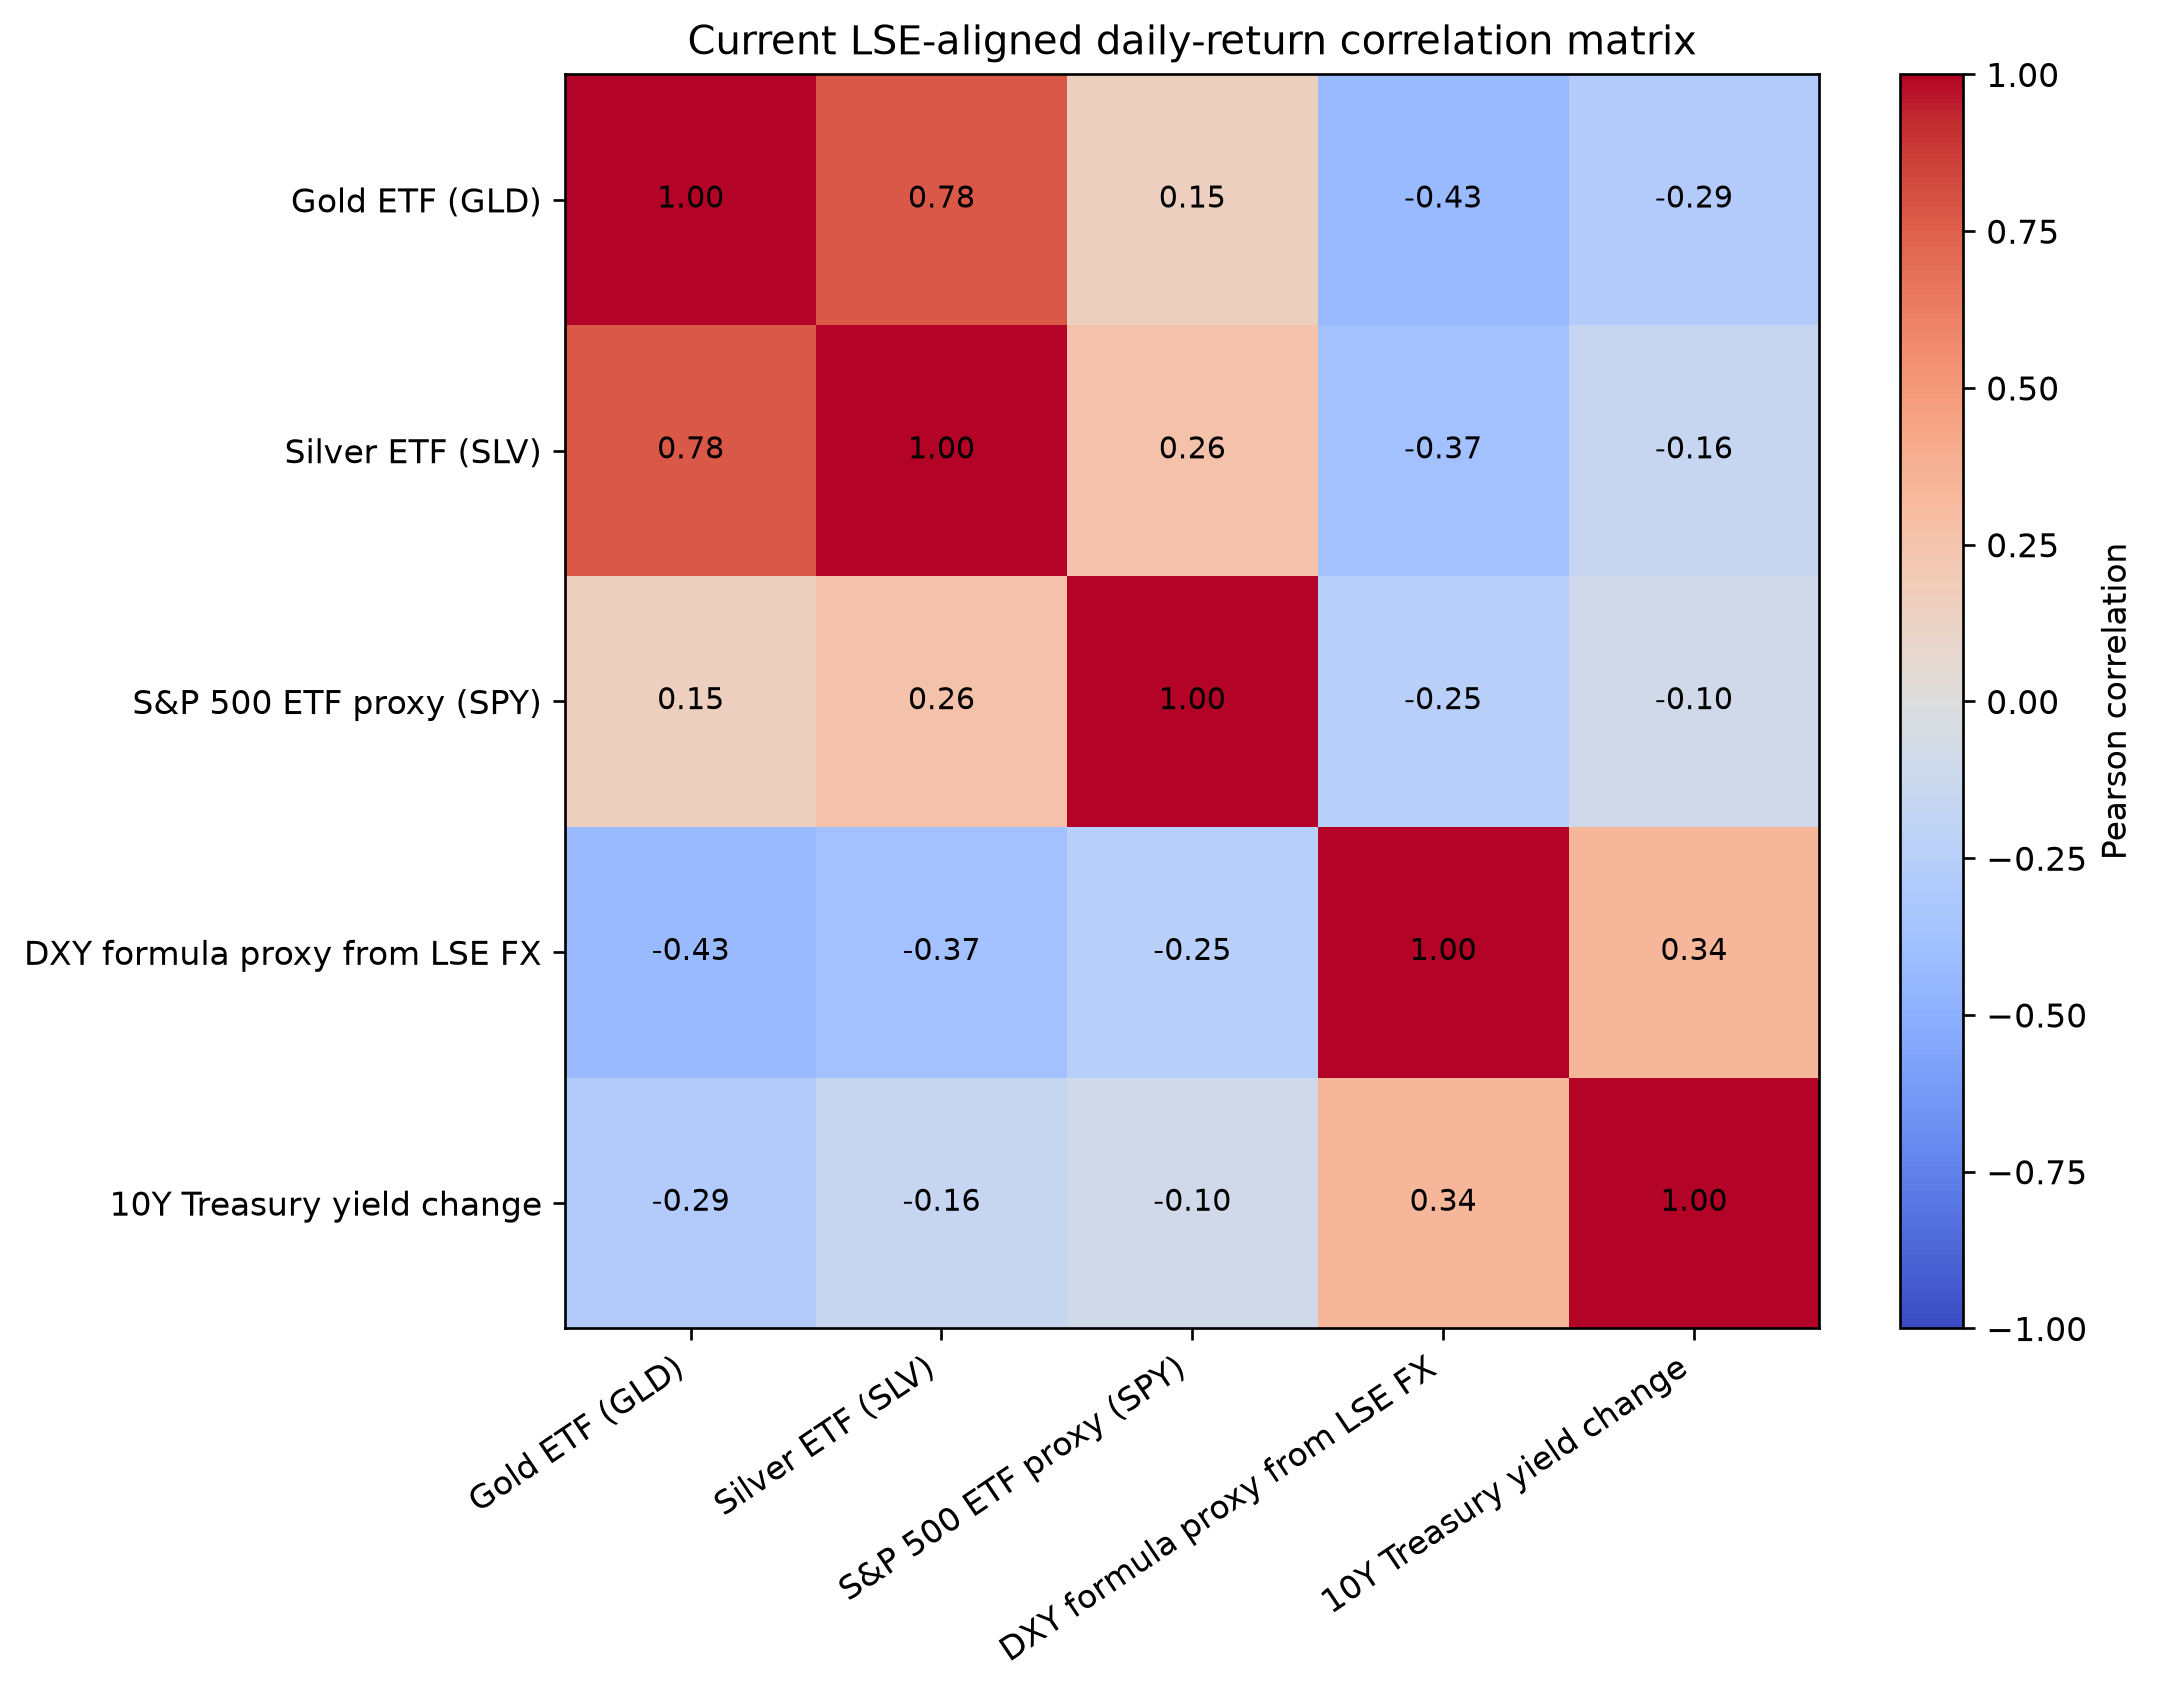
\includegraphics[width=0.82\textwidth]{img/team7_empirical/correlation_heatmap.png}
\caption{Static correlation matrix for the synchronized daily sample}
\label{fig:t7-correlation-heatmap}
\end{figure}

The current LSE matrix in Figure~\ref{fig:t7-correlation-heatmap} reveals
several patterns. GLD and SLV exhibit a strong positive correlation ($0.78$).
GLD is weakly correlated with SPY ($0.15$), while its correlations with the
DXY-formula proxy ($-0.43$) and the change in the 10-year Treasury yield
($-0.29$) are negative. SLV has a larger positive SPY correlation ($0.26$), a
negative dollar-proxy correlation ($-0.37$), and a weaker yield-change
correlation ($-0.16$). These are unconditional sample
associations, not universal hedge coefficients; the rolling evidence below
shows that both sign and magnitude vary through time.
\subsubsection{Linear regression framework}


Building on the correlation analysis discussed above, we next specify linear regression models that relate gold and silver returns to the macro-financial drivers identified in Chapter~2 and formalised econometrically in Chapter~5.
While correlations are symmetric and purely descriptive, regression models impose a
direction of explanation and allow us to condition on multiple variables at once
\sourcecitation{Wooldridge2020}. Following the econometric framework introduced in the theoretical
section on ordinary least squares, we model gold and silver returns as linear functions of
bond, equity, and dollar returns:
\[
r^{gold}_t = \beta_0 + \beta_1 r^{bond}_t + \beta_2 r^{equity}_t
+ \beta_3 r^{usd}_t + u_t,
\]
\[
r^{silver}_t = \gamma_0 + \gamma_1 r^{bond}_t + \gamma_2 r^{equity}_t
+ \gamma_3 r^{usd}_t + v_t,
\]
where $u_t$ and $v_t$ denote error terms capturing all other factors that affect precious–
metal returns but are not explicitly included in the specification. These baseline models
allow us to quantify how gold and silver co–move with fixed–income markets, stock markets,
and the US dollar, holding the other drivers constant.

From a conceptual standpoint, the interpretation of the coefficients can follow two
complementary perspectives. A \emph{causal} interpretation would require strong identifying
assumptions on the error terms and on the absence of omitted variables, as emphasized in
the discussion of the zero conditional mean assumption and omitted variable bias in the
OLS framework. In this paper, we primarily adopt a \emph{predictive} and descriptive
perspective: the coefficients are interpreted as measures of conditional co–movement and as
indicators of hedge and safe–haven properties, rather than as structural causal effects
(see also the distinction between causal and forecasting objectives in standard
econometrics and time–series texts, e.g., \sourcecitation{Wooldridge2020,Tsay2022}).
\subsubsection{Extensions and robustness}

The original article presented volatility modelling as a future extension. In
the unified thesis, part of that agenda is already completed: GARCH evidence is
reported later in this chapter, continuous-time stochastic variance and jumps
are developed in Chapter~8, and option-surface calibration is performed in
Chapter~9. Additional regressors, quantile methods and formal regime or causal
identification remain robustness extensions rather than completed results.

The linear regression framework adopted in this chapter is primarily designed for descriptive and predictive purposes rather than for structural causal inference. The estimated coefficients should therefore be interpreted as measures of conditional comovement and as indicative of hedge or safe-haven behaviour \emph{in our sample and at the daily frequency considered}, under the maintained assumptions on the error term and the chosen set of regressors, rather than as evidence of deep causal effects.


These design choices provide a coherent link between the descriptive correlation analysis,
the linear regression framework, and the volatility models that follow. The following
sections implement this framework empirically, estimating the models for gold and silver
and interpreting the results in light of their proposed roles as hedges, safe havens, and
diversifiers.


\section{Applied Cross-Asset Evidence}

Static correlations conceal economically important changes in sign and
magnitude. Figure~\ref{fig:t7-gold-rolling-correlations} regenerates the three
GLD rolling-correlation series from the current LSE panel. The dollar relation is
predominantly negative, whereas the equity and yield-change relations are more
state dependent. No rolling correlation alone identifies a causal channel.

\begin{figure}[htbp]
\centering
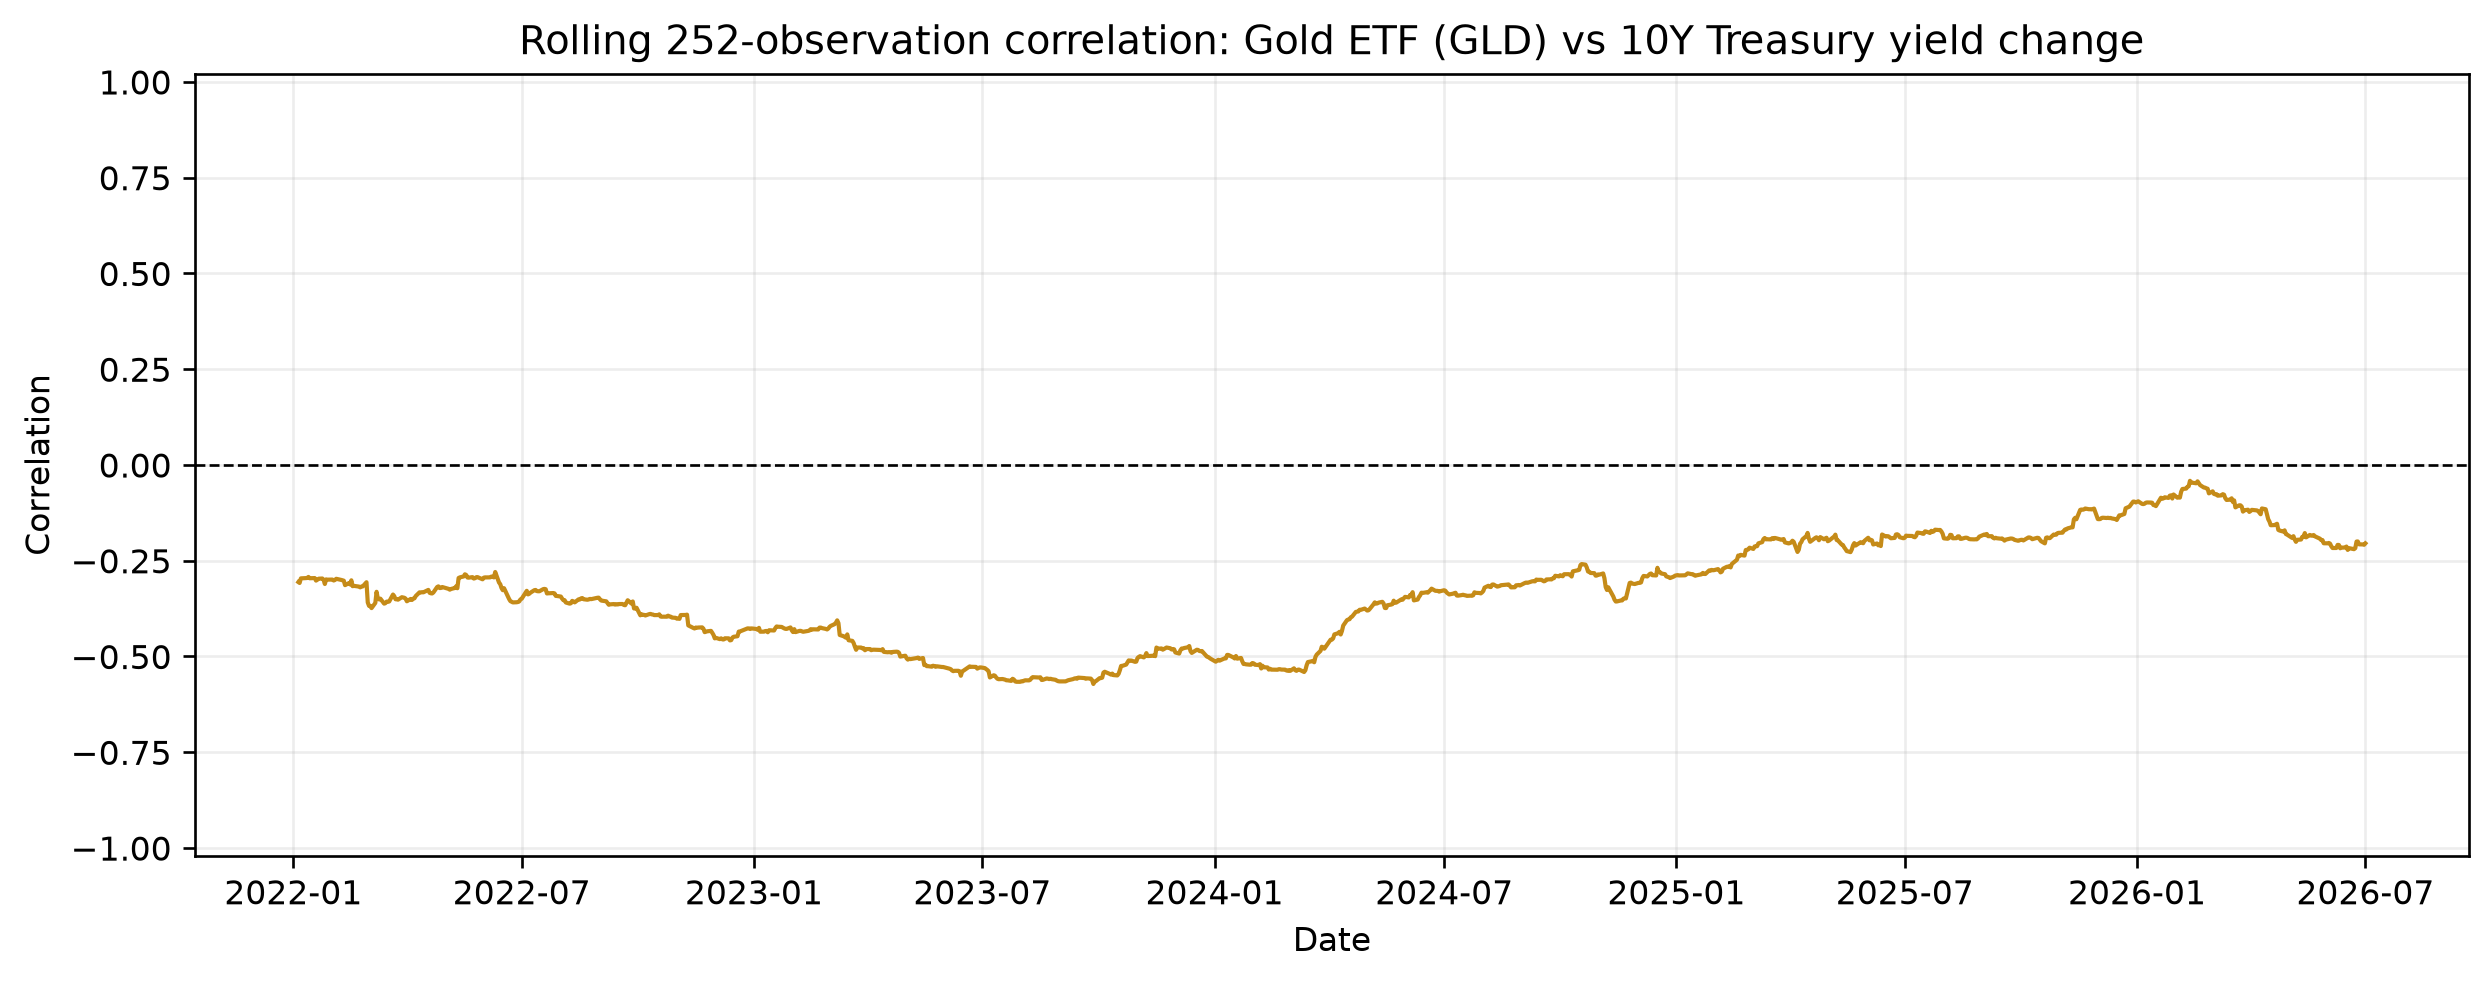
\includegraphics[width=0.88\textwidth]{img/team7_empirical/rolling_corr_gold_ust10y.png}
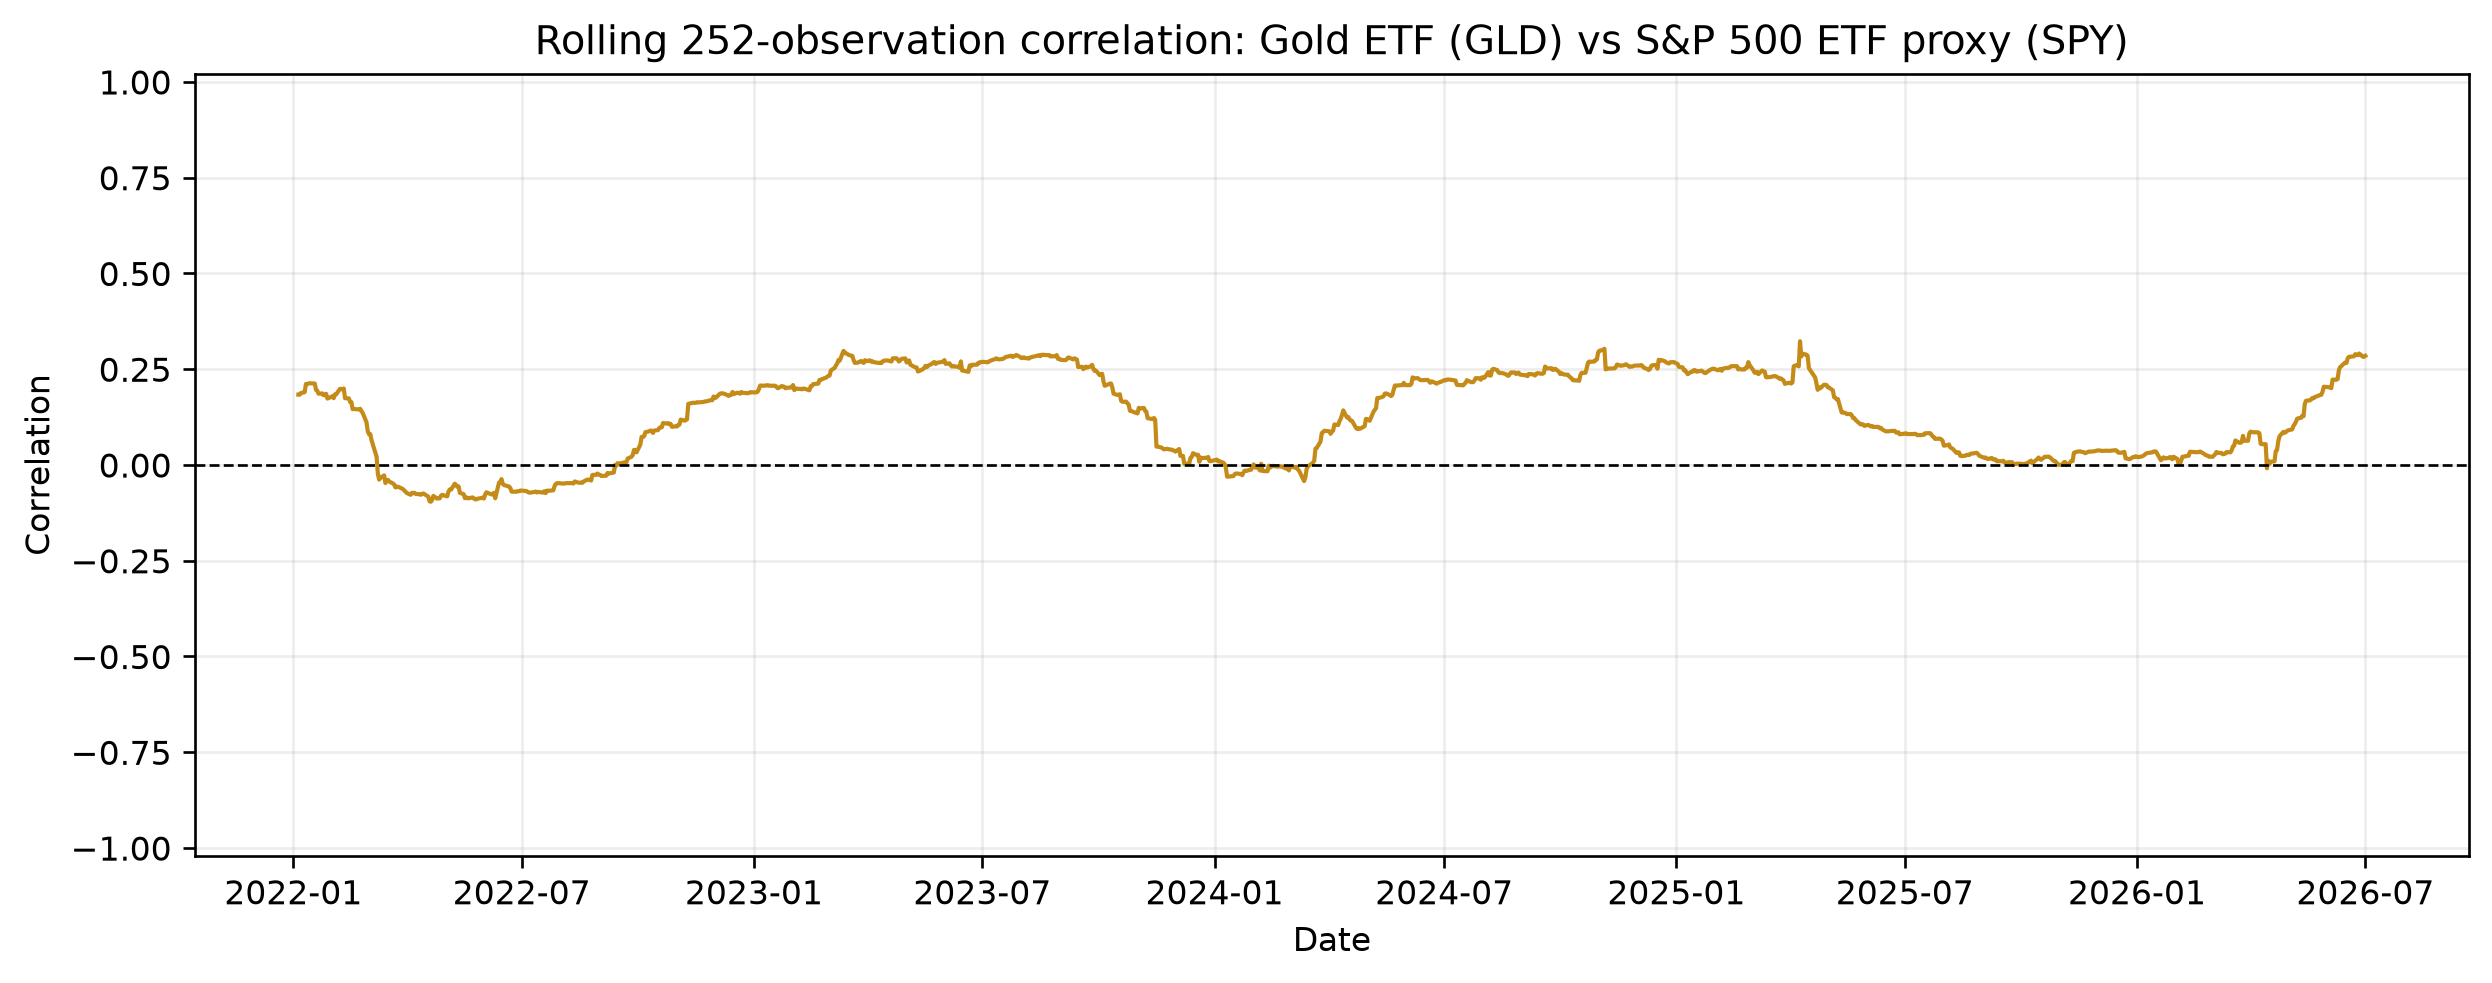
\includegraphics[width=0.88\textwidth]{img/team7_empirical/rolling_corr_gold_sp500.png}
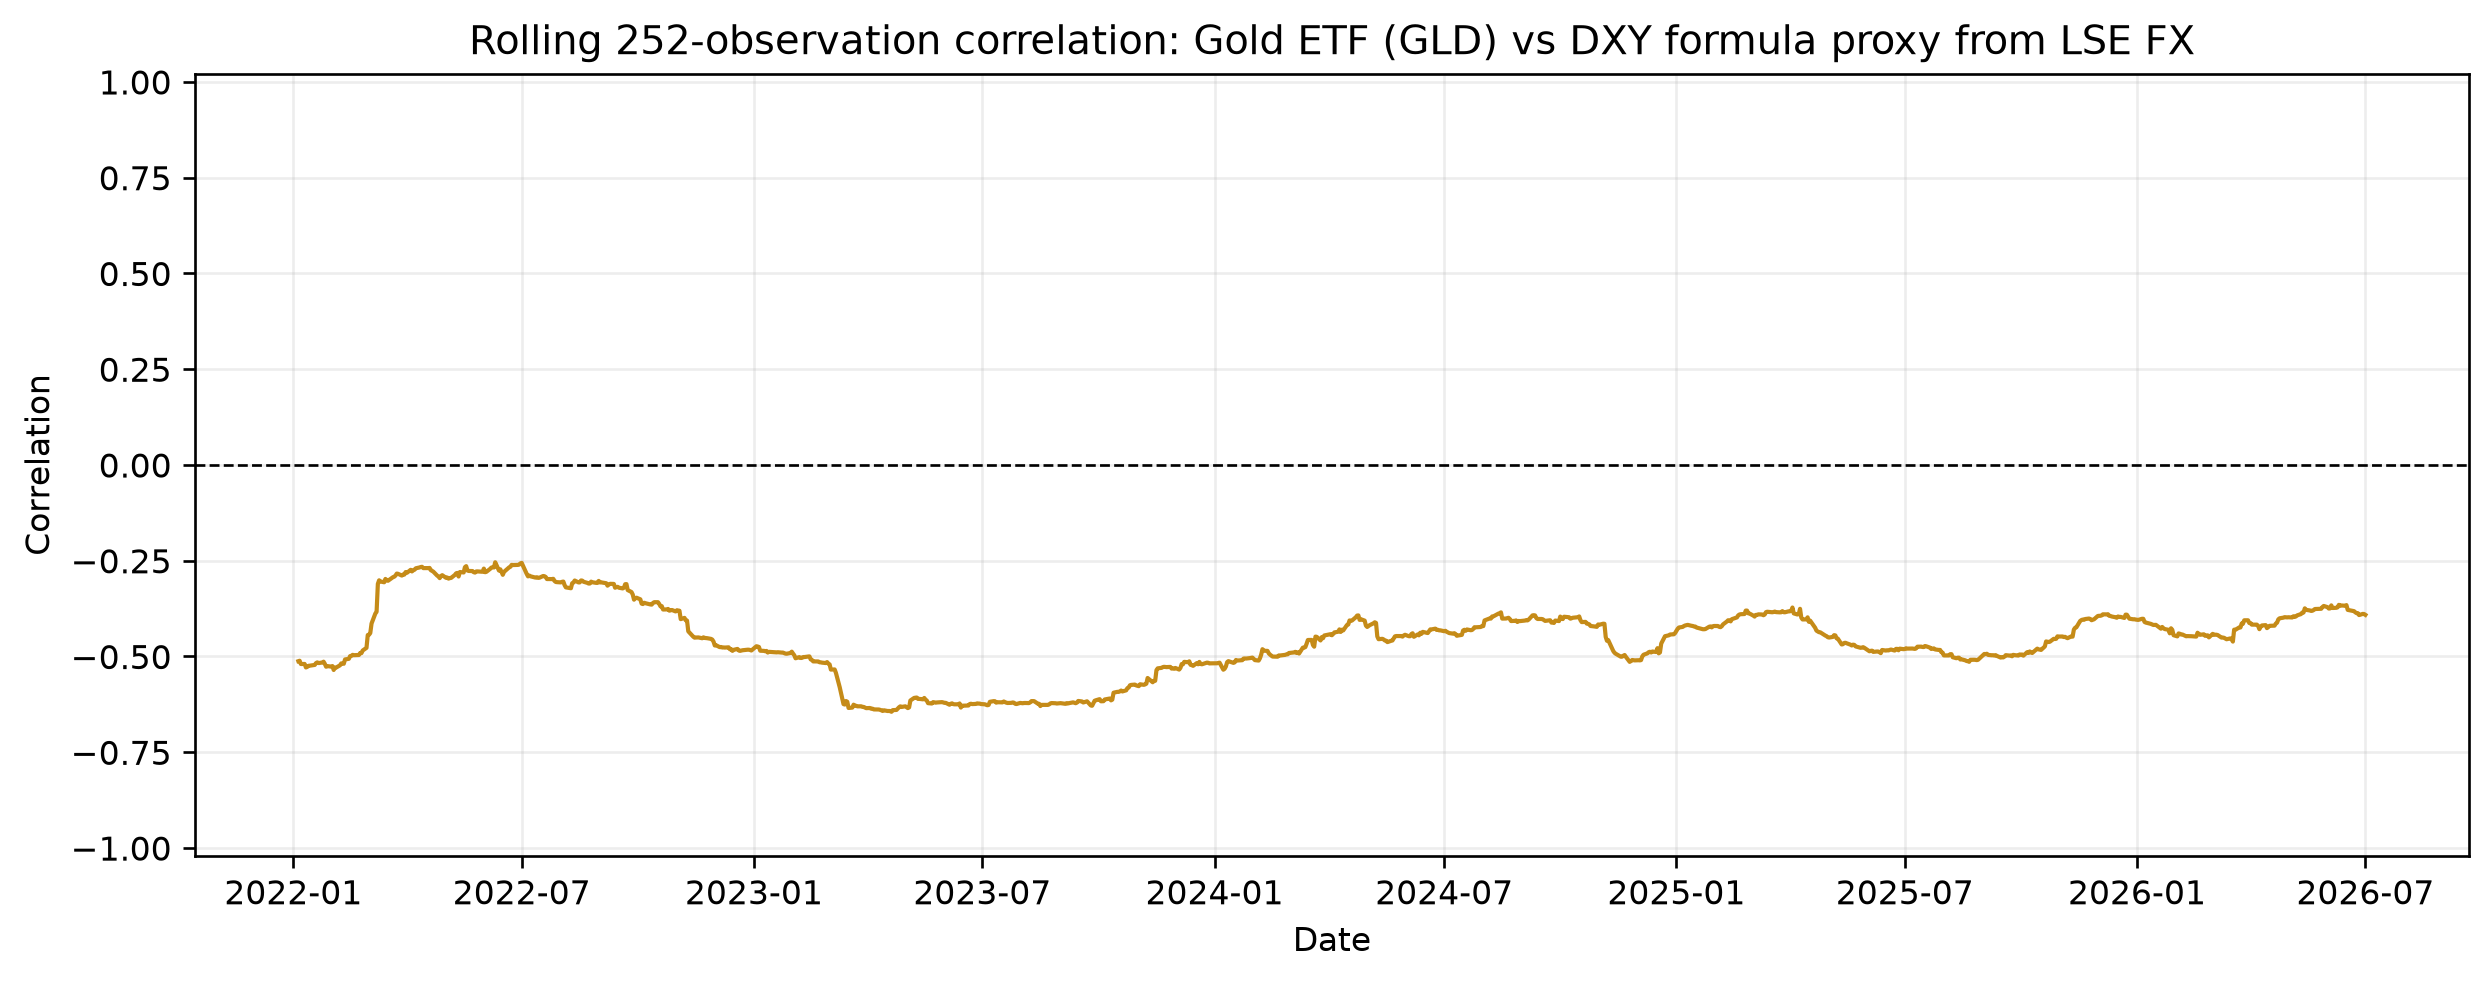
\includegraphics[width=0.88\textwidth]{img/team7_empirical/rolling_corr_gold_dxy.png}
\caption{Rolling 252-observation correlations of GLD returns with LSE
Treasury-yield changes, SPY returns and the transparent DXY-formula proxy}
\label{fig:t7-gold-rolling-correlations}
\end{figure}

The regression estimates in Table~\ref{tab:t7-gold-ols} quantify these
associations. Individually, gold loads negatively on yield changes and DXY;
the single-factor equity coefficient is small and positive. In the joint
specification, the DXY and yield-change coefficients remain statistically
different from zero, while the equity coefficient does not. The dollar factor
accounts for most of the reported explanatory power.

\begin{table}[htbp]
\centering
\caption{Gold-return regressions in the Team~7 sample}
\label{tab:t7-gold-ols}
\small
\begin{tabular}{lrrrr}
\toprule
 & Yield only & Equity only & Dollar only & Joint \\
\midrule
Yield change & $-0.0375^{***}$ & --- & --- & $-0.0292^{***}$ \\
             & $(0.0039)$      &     &     & $(0.0036)$       \\
S\&P 500 return & --- & $0.0506^{**}$ & --- & $0.0224$ \\
                &     & $(0.0250)$    &     & $(0.0250)$ \\
DXY return   & --- & --- & $-0.9810^{***}$ & $-0.9248^{***}$ \\
             &     &     & $(0.0450)$       & $(0.0466)$       \\
Constant     & $0.0003^{*}$ & $0.0003$ & $0.0003^{**}$ & $0.0003^{**}$ \\
             & $(0.0002)$   & $(0.0002)$& $(0.0001)$    & $(0.0001)$    \\
\midrule
$N$          & 4,694 & 4,694 & 4,694 & 4,694 \\
$R^2$        & 0.038 & 0.003 & 0.176 & 0.197 \\
Adjusted $R^2$ & 0.0376 & 0.0026 & 0.1760 & 0.1961 \\
\bottomrule
\end{tabular}
\begin{minipage}{0.92\textwidth}
\footnotesize\emph{Notes:} Heteroskedasticity-robust HC1 standard errors in
parentheses. $^{*}p<0.10$, $^{**}p<0.05$, $^{***}p<0.01$.
\end{minipage}
\end{table}

Silver provides a useful comparator rather than a substitute for gold. Its
rolling relations in Figure~\ref{fig:t7-silver-rolling-correlations} are more
equity-sensitive and remain time varying. In the joint regressions, silver's
equity loading is $0.2625$ (robust standard error $0.0424$), compared with
$0.0224$ ($0.0250$) for gold; the dollar loadings are $-1.6229$ ($0.0860$)
and $-0.9248$ ($0.0466$), respectively. The joint $R^2$ values are $0.205$
for silver and $0.197$ for gold.

\begin{table}[htbp]
\centering
\caption{Silver-return regressions in the Team~7 sample}
\label{tab:t7-silver-ols}
\small
\begin{tabular}{lrrrr}
\toprule
 & Yield only & Equity only & Dollar only & Joint \\
\midrule
Yield change & $-0.0206^{***}$ & --- & --- & $-0.0201^{***}$ \\
             & $(0.0067)$      &     &     & $(0.0062)$       \\
S\&P 500 return & --- & $0.3543^{***}$ & --- & $0.2625^{***}$ \\
                &     & $(0.0408)$     &     & $(0.0424)$       \\
DXY return   & --- & --- & $-1.7854^{***}$ & $-1.6229^{***}$ \\
             &     &     & $(0.0789)$        & $(0.0860)$        \\
Constant     & $0.0001$ & $0.0000$ & $0.0002$ & $0.0001$ \\
             & $(0.0002)$& $(0.0003)$& $(0.0002)$& $(0.0002)$ \\
\midrule
$N$          & 4,694 & 4,694 & 4,694 & 4,694 \\
$R^2$        & 0.004 & 0.049 & 0.182 & 0.205 \\
Adjusted $R^2$ & 0.0030 & 0.0485 & 0.1810 & 0.2050 \\
\bottomrule
\end{tabular}
\begin{minipage}{0.92\textwidth}
\footnotesize\emph{Notes:} Heteroskedasticity-robust HC1 standard errors in
parentheses. $^{*}p<0.10$, $^{**}p<0.05$, $^{***}p<0.01$.
\end{minipage}
\end{table}

\begin{figure}[htbp]
\centering
\begin{minipage}{0.49\textwidth}
\centering
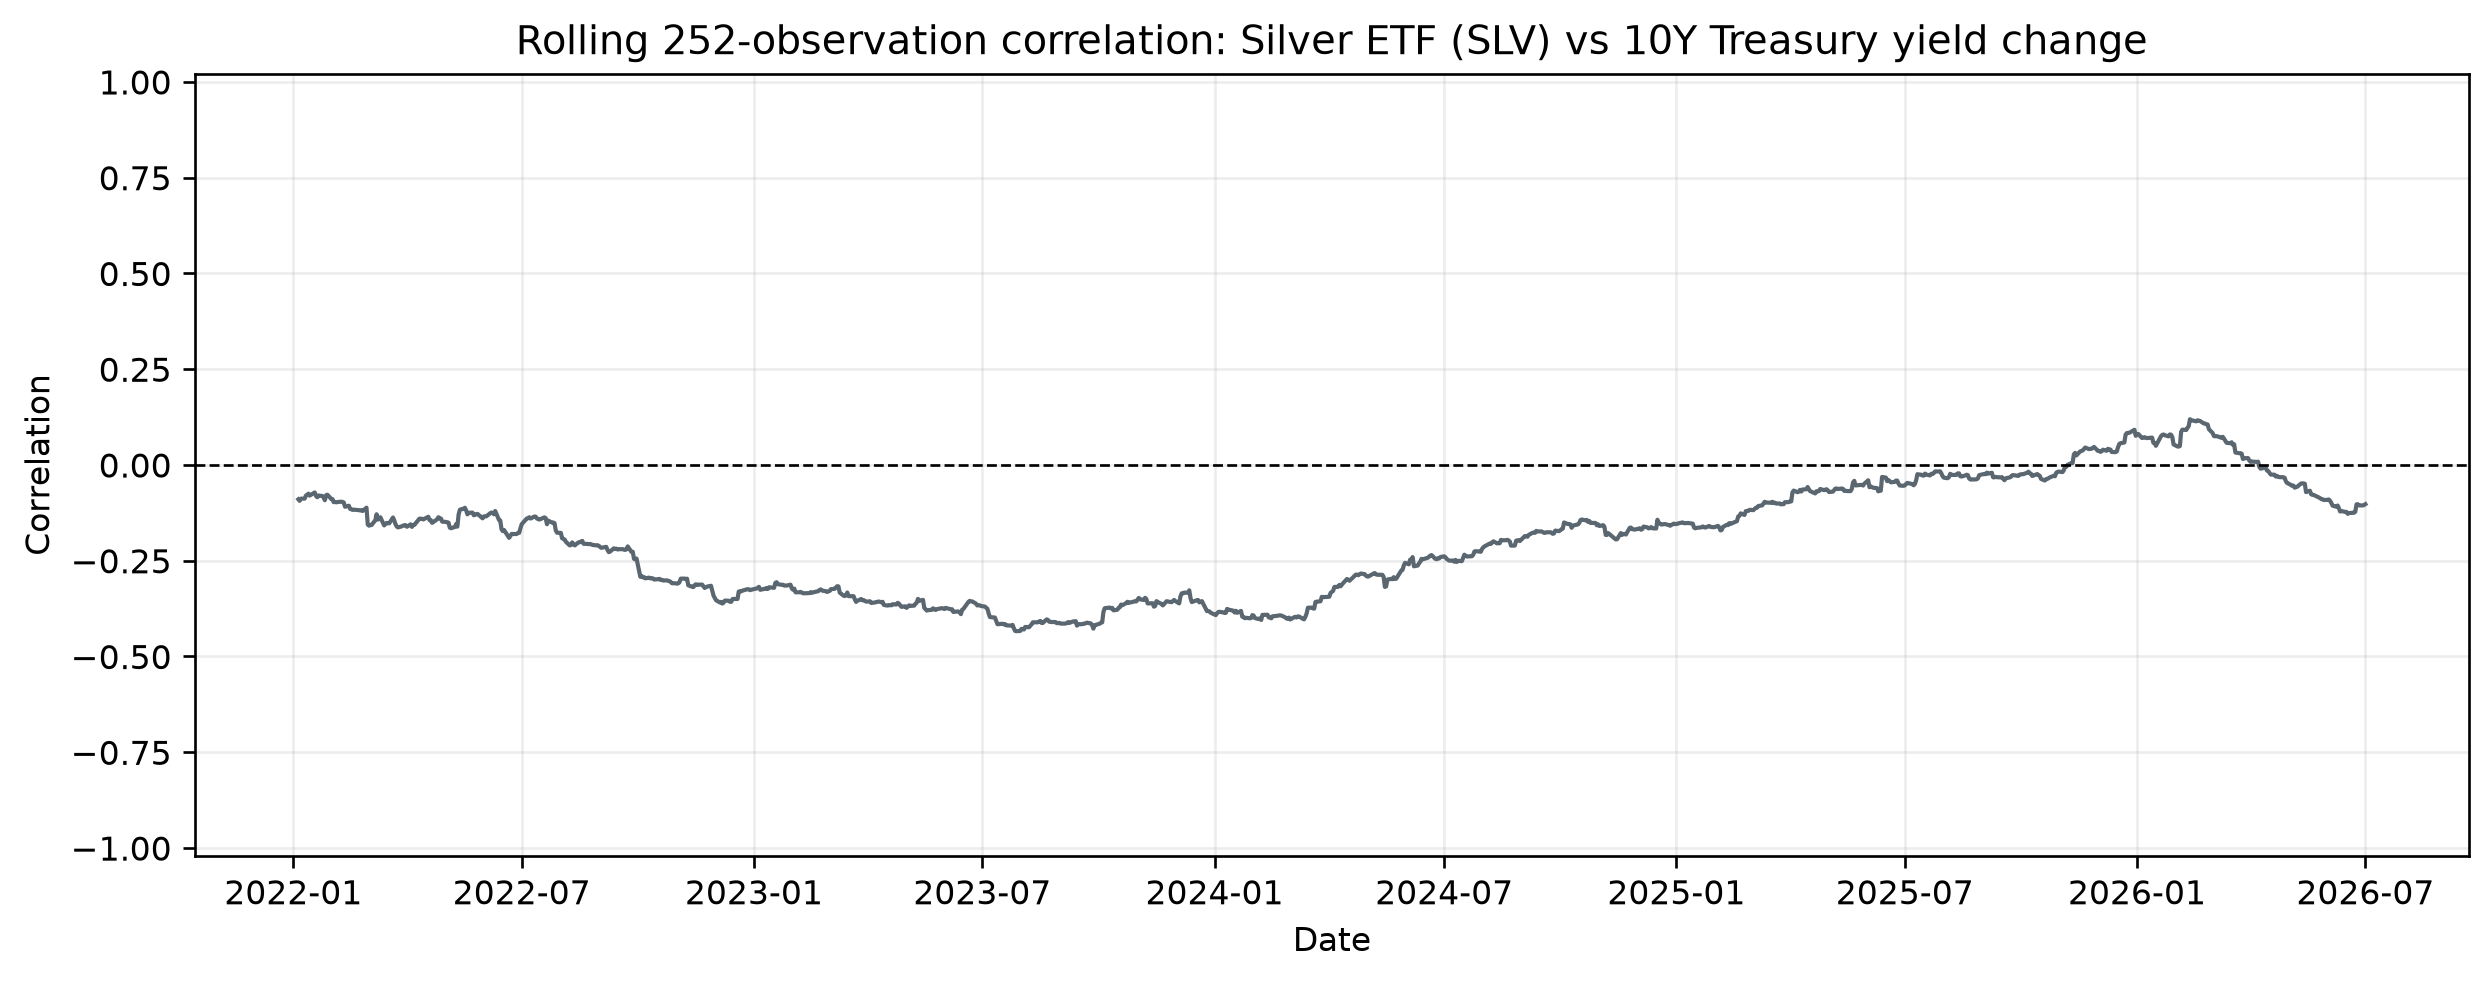
\includegraphics[width=\linewidth]{img/team7_empirical/rolling_corr_silver_ust10y.png}
\end{minipage}\hfill
\begin{minipage}{0.49\textwidth}
\centering
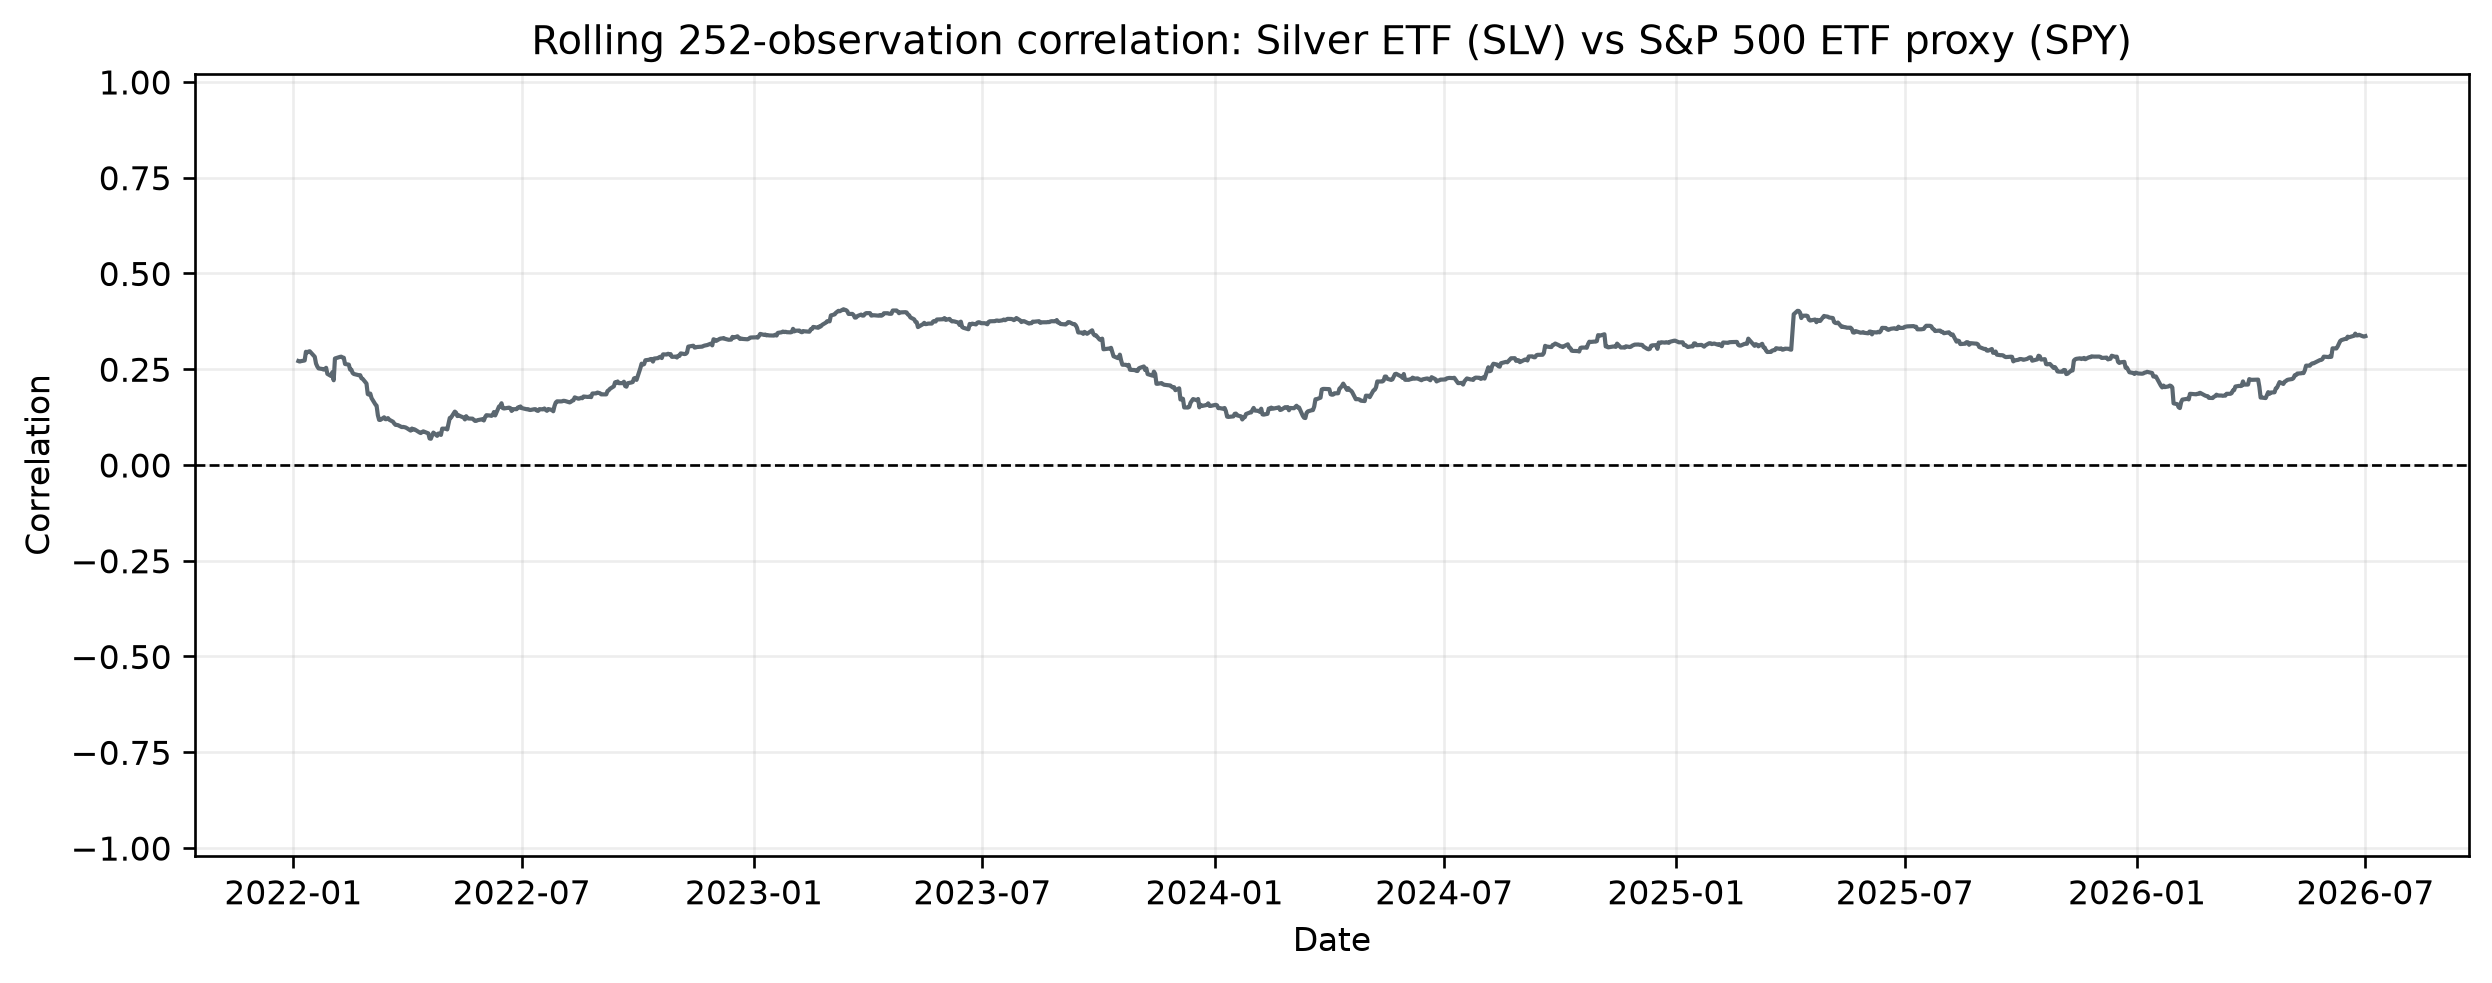
\includegraphics[width=\linewidth]{img/team7_empirical/rolling_corr_silver_sp500.png}
\end{minipage}

\begin{minipage}{0.55\textwidth}
\centering
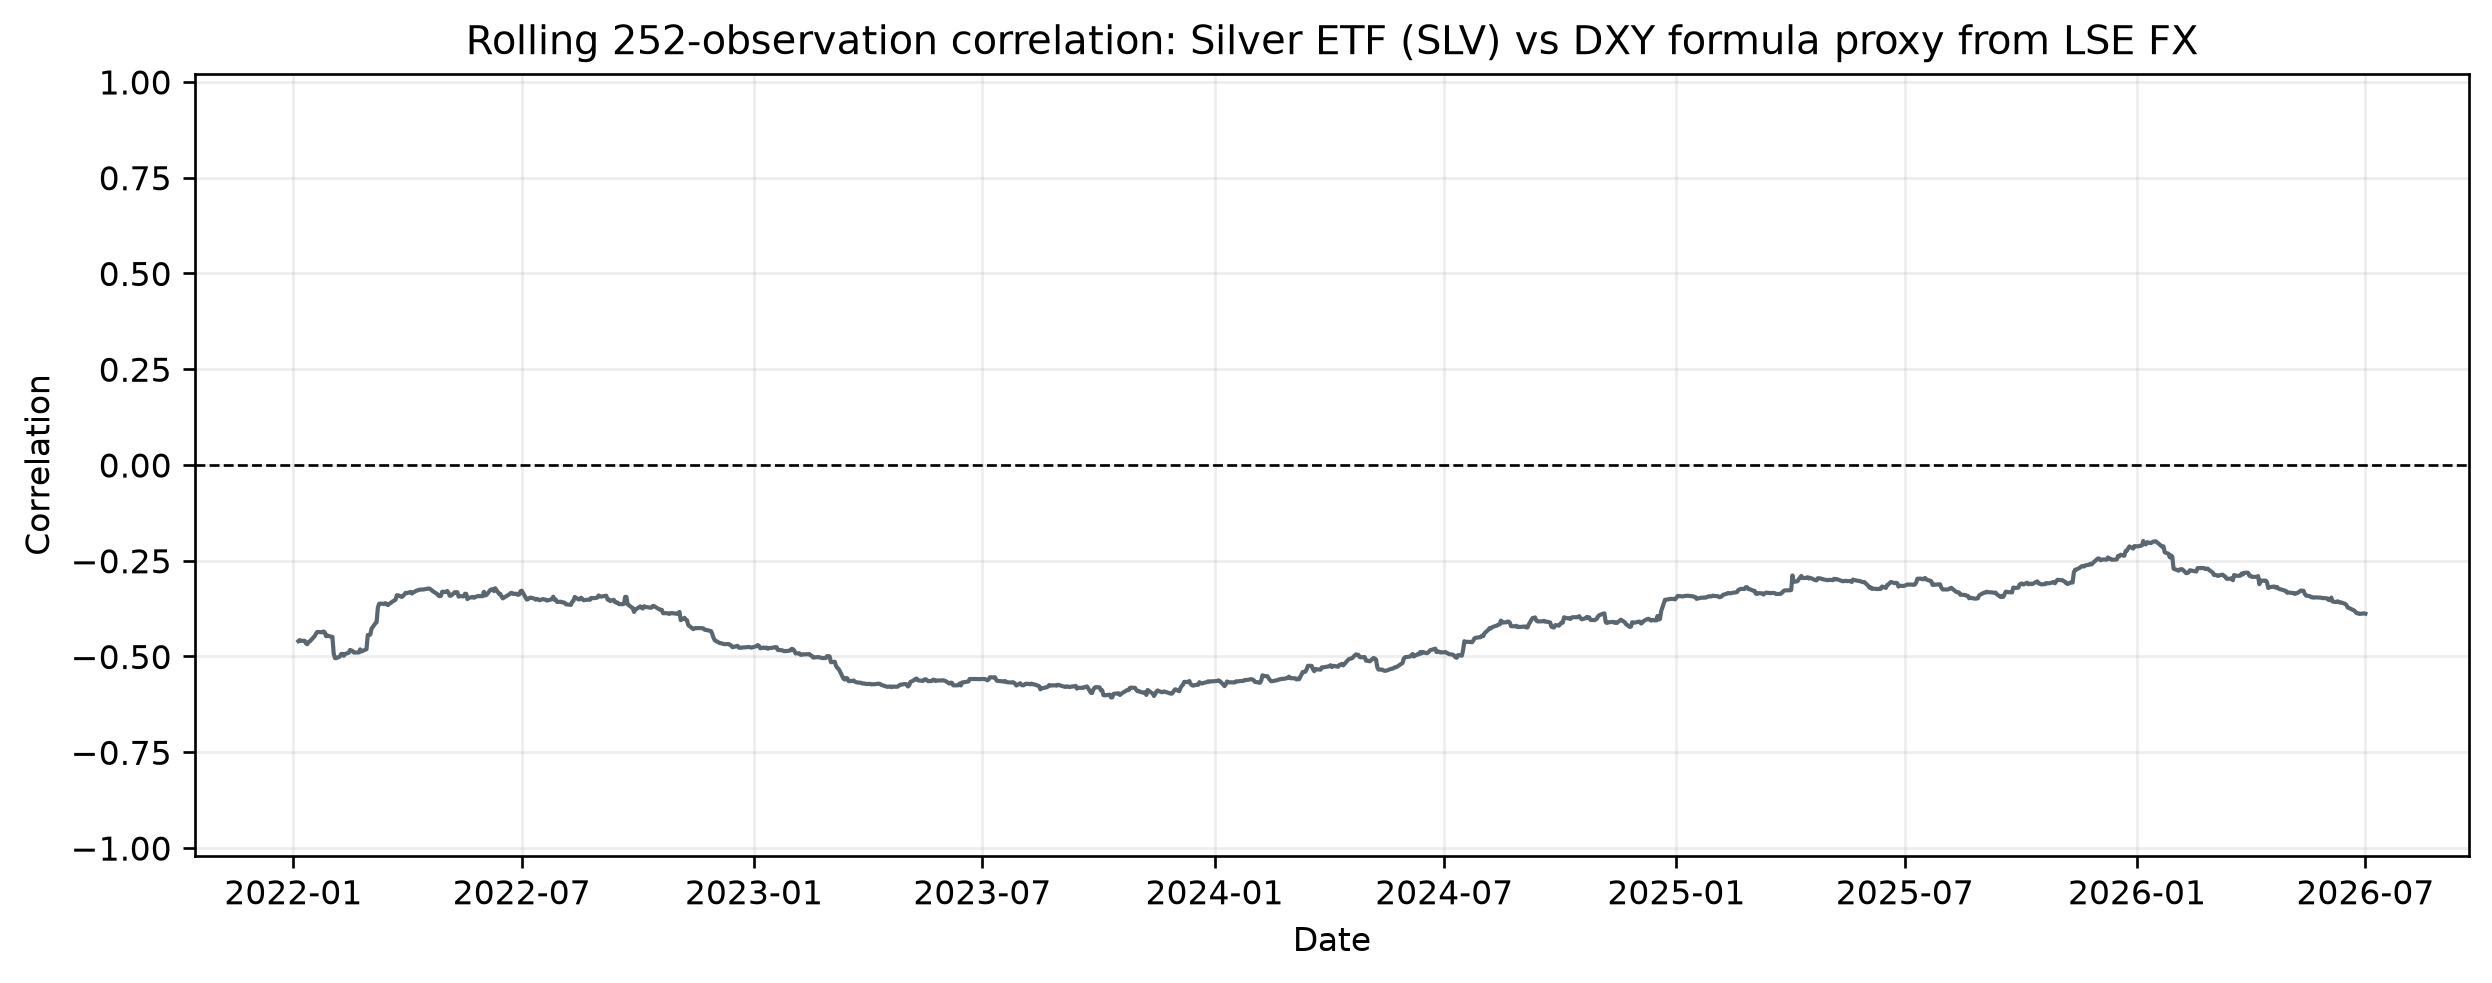
\includegraphics[width=\linewidth]{img/team7_empirical/rolling_corr_silver_dxy.png}
\end{minipage}
\caption{Rolling 252-observation correlations of SLV returns with LSE
Treasury-yield changes, SPY returns and the transparent DXY-formula proxy}
\label{fig:t7-silver-rolling-correlations}
\end{figure}

The combined evidence supports three limited conclusions. Gold and silver are
strongly related but silver is materially more volatile; gold's unconditional
equity relationship is weak; and the negative dollar relationship is much
more stable than the bond-yield or equity relations. The evidence motivates
state-dependent volatility modelling, but it does not establish a universal
safe-haven law.

\section{Log Prices, Returns and Stationarity}

The distinction between log-price levels and log returns governs the model
choice. Log prices are highly persistent and empirically close to a unit-root
process, whereas daily returns are much closer to weak stationarity. An AR(1)
fit to price levels consequently produces coefficients near one and very high
in-sample explanatory power: approximately $0.9993$ for gold with
$R^2\approx0.999$, and $0.9978$ for silver with $R^2\approx0.996$. These values
primarily record persistence and must not be read as useful economic
forecastability.

For returns, the same benchmark changes sharply. The estimated AR(1)
coefficient is approximately $-0.0024$ for gold and $0.0063$ for silver, with
robust standard errors near $0.0202$ and $0.0227$ and essentially zero
$R^2$. At the daily frequency the conditional mean is therefore weak even
though the price level is persistent.

\begin{table}[htbp]
\centering
\caption{AR(1) contrast between log-price levels and daily returns}
\label{tab:t7-ar1-level-return}
\small
\begin{tabular}{llrrrr}
\toprule
Asset & Dependent series & $\hat\phi_1$ & Robust s.e. & $t$-statistic & $R^2$ \\
\midrule
Gold   & Log price & 0.9993  & 0.0006 & 1653.18 & 0.9987 \\
Silver & Log price & 0.9978  & 0.0012 &  802.26 & 0.9956 \\
Gold   & Return    &-0.0024  & 0.0202 &   -0.12 & 0.0000 \\
Silver & Return    & 0.0063  & 0.0227 &    0.28 & 0.0000 \\
\bottomrule
\end{tabular}
\begin{minipage}{0.90\textwidth}
\footnotesize\emph{Notes:} Values reproduce the published Team~7 article
snapshot. High fit in levels reflects near-unit-root persistence, not reliable
return predictability.
\end{minipage}
\end{table}

\section{AR, ARMA and ARIMA Diagnostics}

Higher-order autoregressions do not overturn the AR(1) result. AIC and BIC
select low-dimensional specifications and the joint lag tests provide little
evidence that lagged daily returns explain current returns. ARMA searches also
remain parsimonious and are not stable enough across criteria to reveal a
substantive conditional-mean law.

\begin{table}[htbp]
\centering
\caption{Higher-order autoregressive diagnostics for daily returns}
\label{tab:t7-arp-diagnostics}
\small
\begin{tabular}{lrrrrr}
\toprule
Asset & AIC lag & BIC lag & $R^2$ & Joint $F$ & $p$-value \\
\midrule
Gold   & 1 & 1 & 0.000006 & 0.0144 & 0.9046 \\
Silver & 1 & 1 & 0.000040 & 0.0779 & 0.7801 \\
\bottomrule
\end{tabular}
\end{table}

ARIMA is not rejected because prices are non-stationary: differencing is
precisely how the model addresses that feature. On log prices, the legacy
selection produces ARIMA$(2,1,0)$ by AIC and ARIMA$(0,1,1)$ by BIC for gold;
for silver both criteria select ARIMA$(1,1,0)$. Once differenced, these models
are close to the simple ARMA descriptions of returns and add little predictive
structure at the horizon considered.

\begin{table}[htbp]
\centering
\caption{Information-criterion selections for ARMA returns and ARIMA log prices}
\label{tab:t7-arma-arima-selection}
\small
\begin{tabular}{lllrr}
\toprule
Asset & Series and criterion & Selected order & AIC & BIC \\
\midrule
Gold   & Return, AIC      & ARMA$(2,0)$  & -28,909.4140 & --- \\
Gold   & Return, BIC      & ARMA$(0,1)$  & --- & -28,889.9939 \\
Silver & Return, AIC/BIC  & ARMA$(1,0)$  & -23,448.9424 & -23,429.5802 \\
Gold   & Log price, AIC   & ARIMA$(2,1,0)$ & -28,909.4140 & --- \\
Gold   & Log price, BIC   & ARIMA$(0,1,1)$ & --- & -28,889.9939 \\
Silver & Log price, AIC/BIC & ARIMA$(1,1,0)$ & -23,448.9424 & -23,429.5802 \\
\bottomrule
\end{tabular}
\begin{minipage}{0.94\textwidth}
\footnotesize\emph{Notes:} The equality of several ARMA and ARIMA criteria is
expected because first-differenced log prices are the return series. Dashes
mark the criterion not used for the stated selection.
\end{minipage}
\end{table}

\section{Heavy Tails, Clustering and Persistence}

The return distribution shifts attention from the conditional mean to the
second moment and the tails. In the frozen 2006--2024 table layer, daily standard deviation
is approximately $1.1\%$ for gold and $2.0\%$ for silver. Estimated skewness is
about $-0.33$ and $-0.85$, while excess kurtosis is approximately $6.25$ and
$7.79$. Gaussian innovations therefore understate the frequency and asymmetry
of large moves, especially for silver.

\begin{table}[htbp]
\centering
\caption{Distributional moments of daily precious-metal returns}
\label{tab:t7-return-moments}
\small
\begin{tabular}{lrrrrr}
\toprule
Asset & Mean & Std. dev. & Skewness & Excess kurtosis & Kurtosis \\
\midrule
Gold   & 0.00028 & 0.01112 & -0.33 & 6.25 & 9.25 \\
Silver & 0.00014 & 0.01990 & -0.85 & 7.79 & 10.79 \\
\bottomrule
\end{tabular}
\end{table}

Figures~\ref{fig:t7-return-histograms} and
\ref{fig:t7-return-qqplots}, regenerated on current LSE GLD/SLV returns, make
the departure from Gaussianity visible. The
centre is sharper than the fitted normal density and both tails contain more
mass; the Q--Q deviations are especially pronounced for silver.

\begin{figure}[htbp]
\centering
\begin{minipage}{0.49\textwidth}
\centering
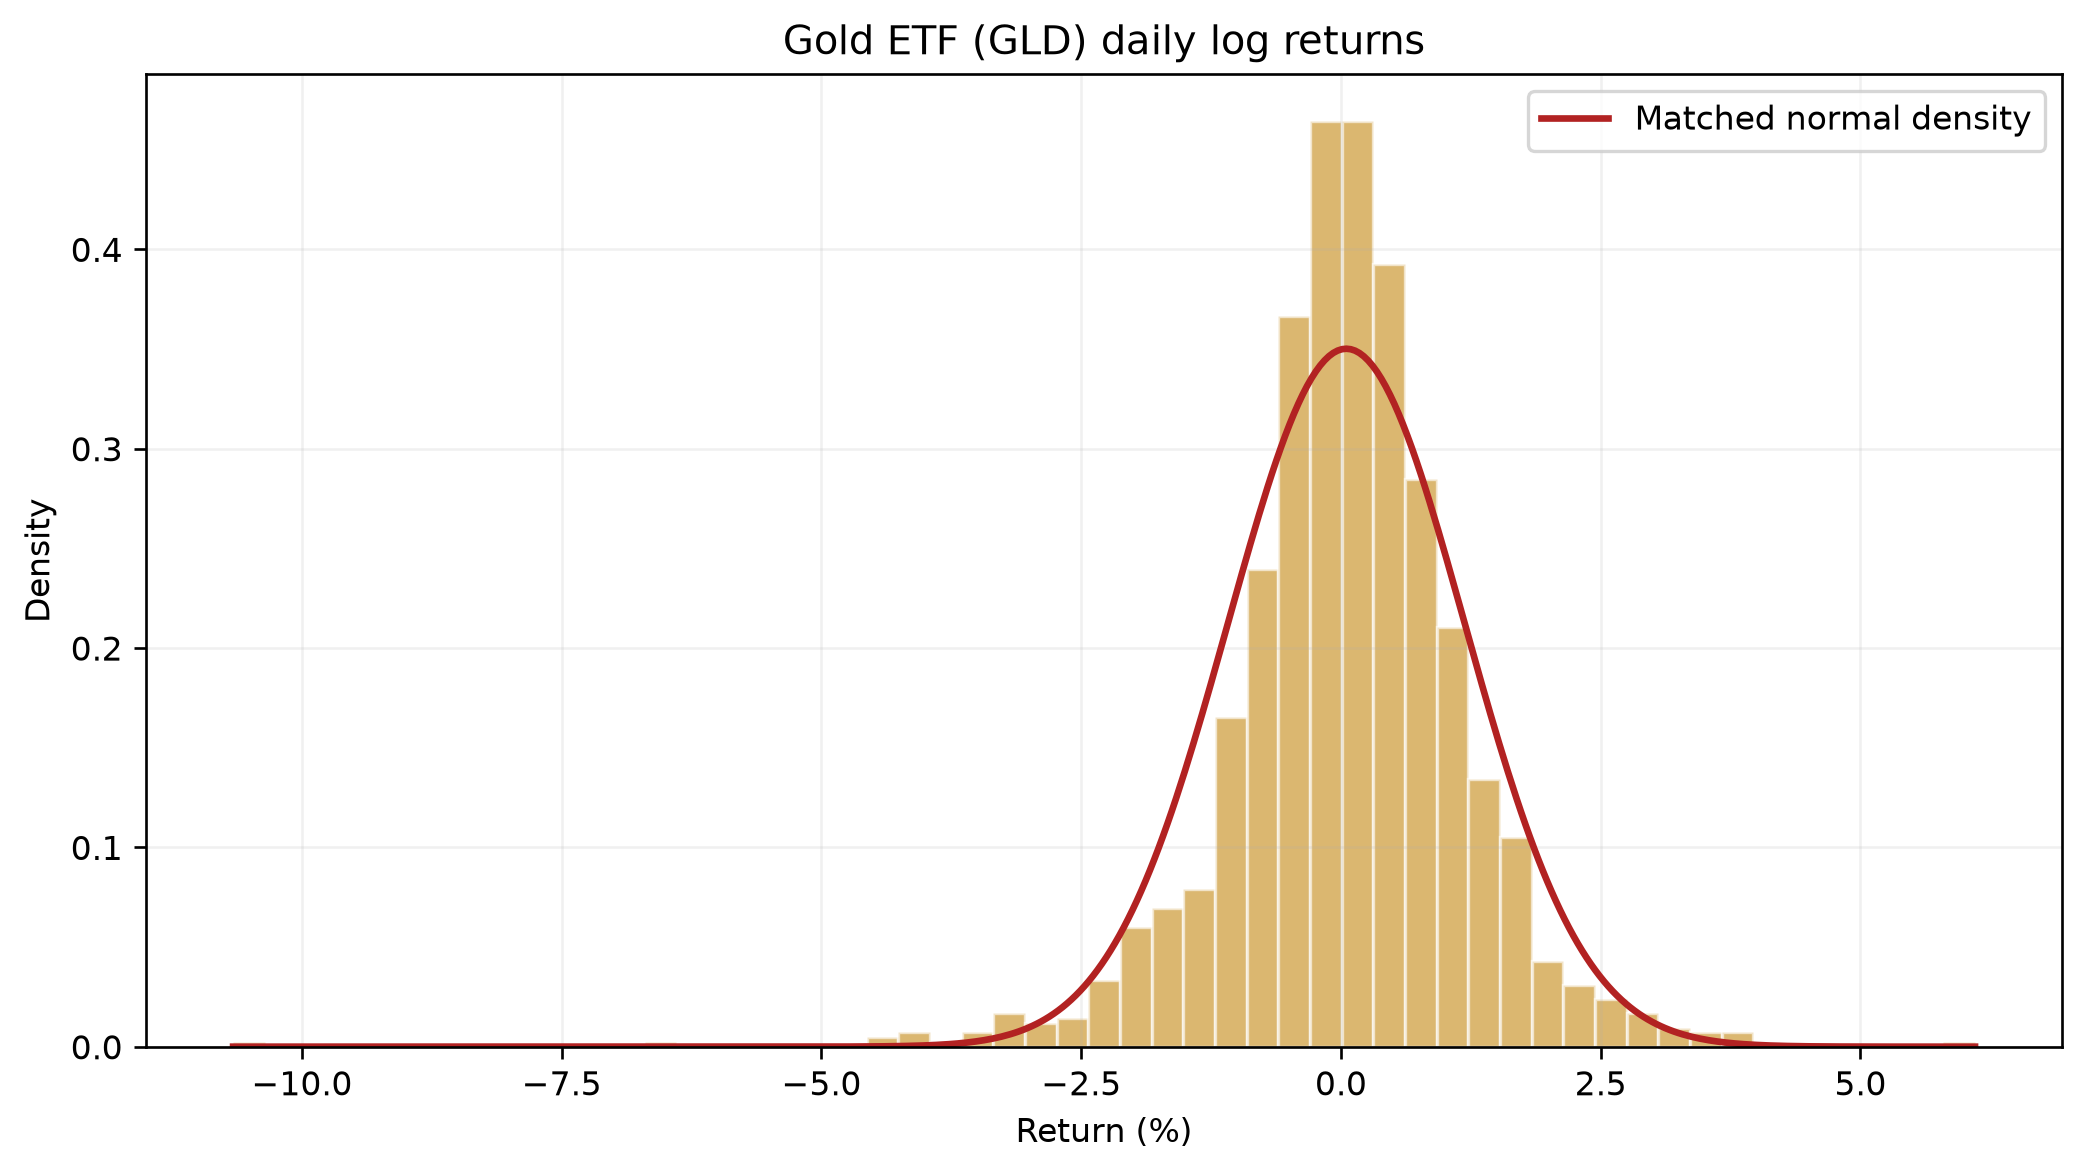
\includegraphics[width=\linewidth]{img/team7_empirical/hist_normal_gold.png}
\end{minipage}\hfill
\begin{minipage}{0.49\textwidth}
\centering
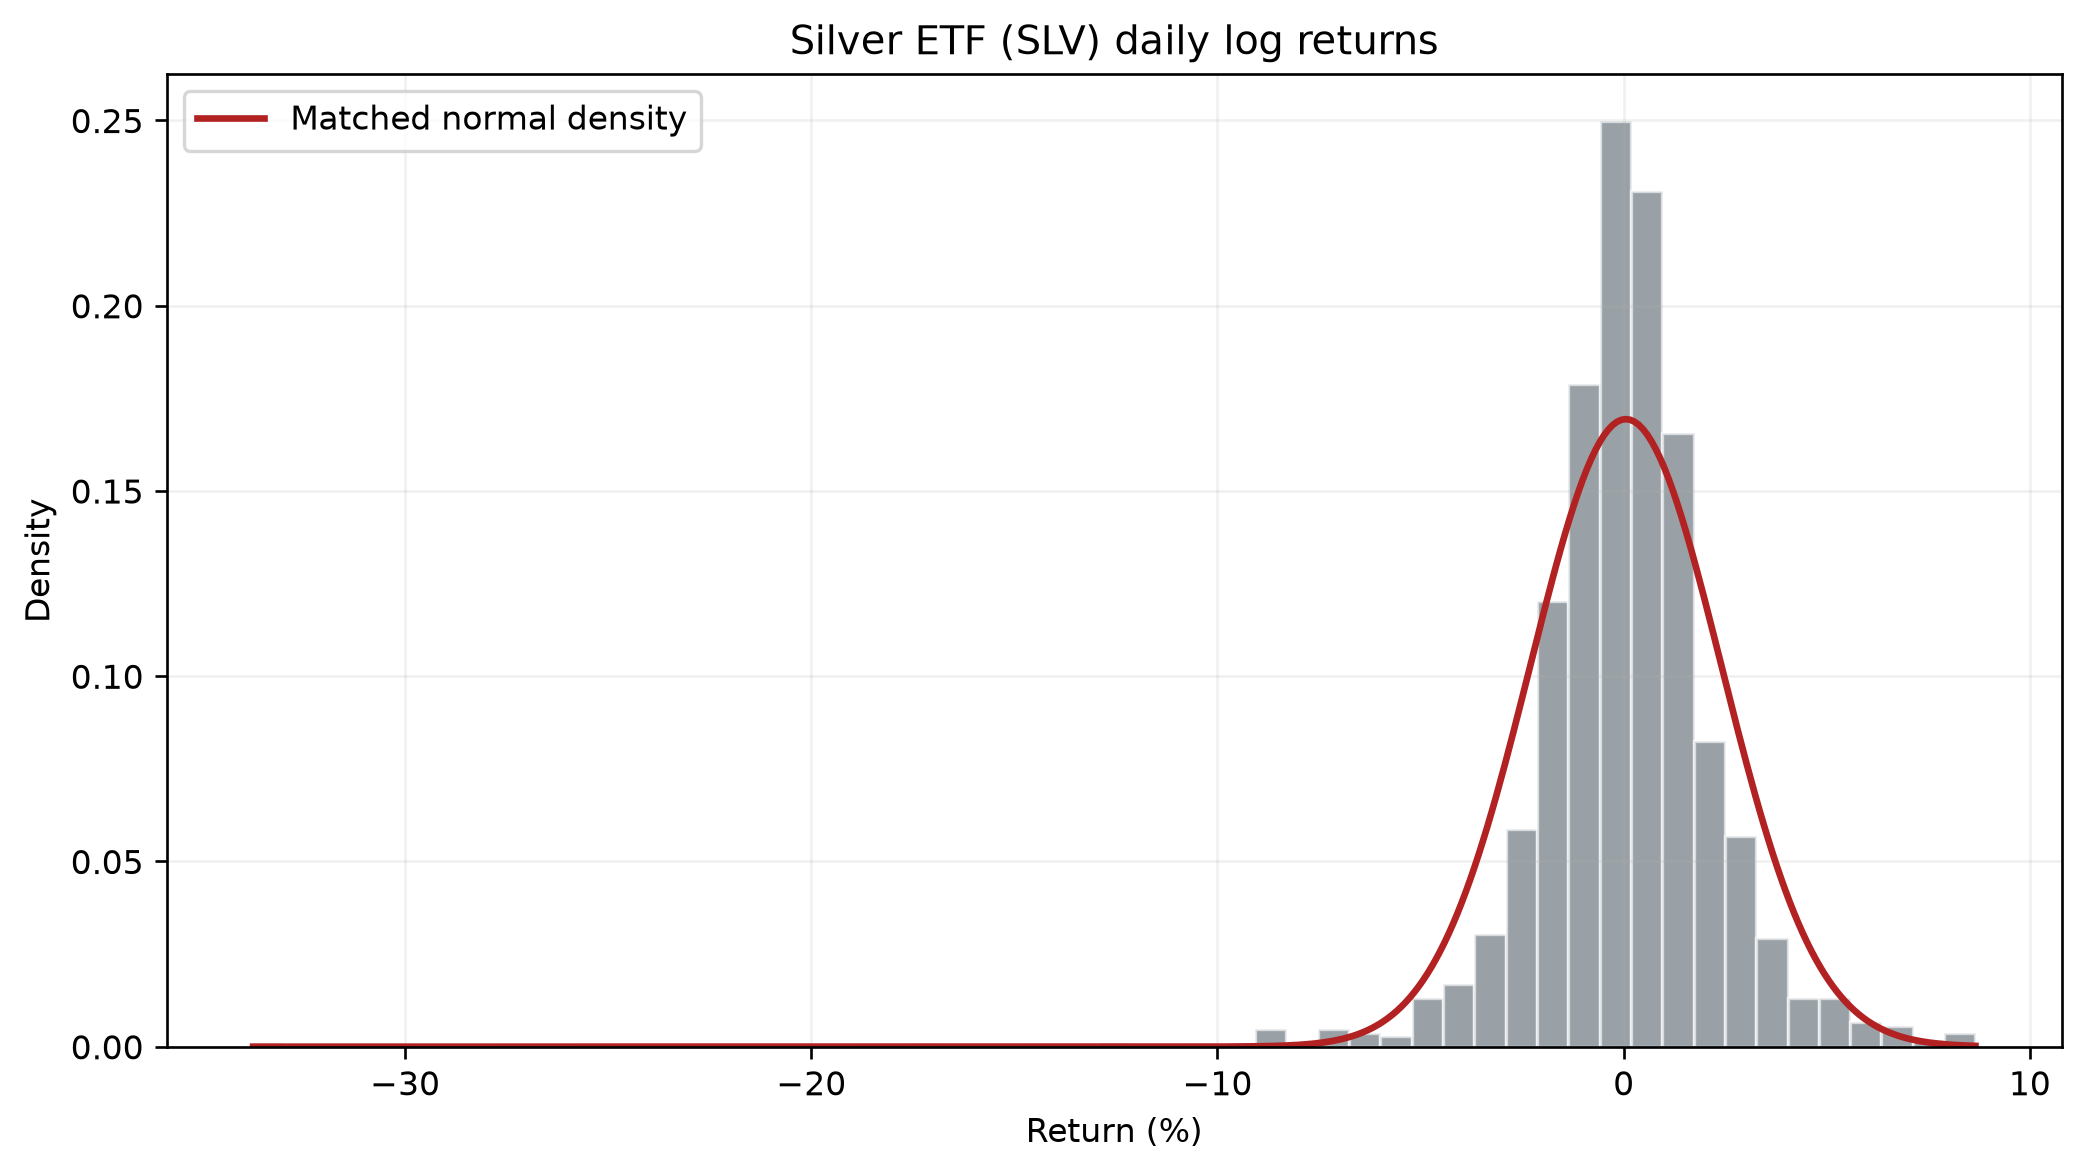
\includegraphics[width=\linewidth]{img/team7_empirical/hist_normal_silver.png}
\end{minipage}
\caption{Current LSE GLD and SLV return histograms with matched normal benchmarks}
\label{fig:t7-return-histograms}
\end{figure}

\begin{figure}[htbp]
\centering
\begin{minipage}{0.49\textwidth}
\centering
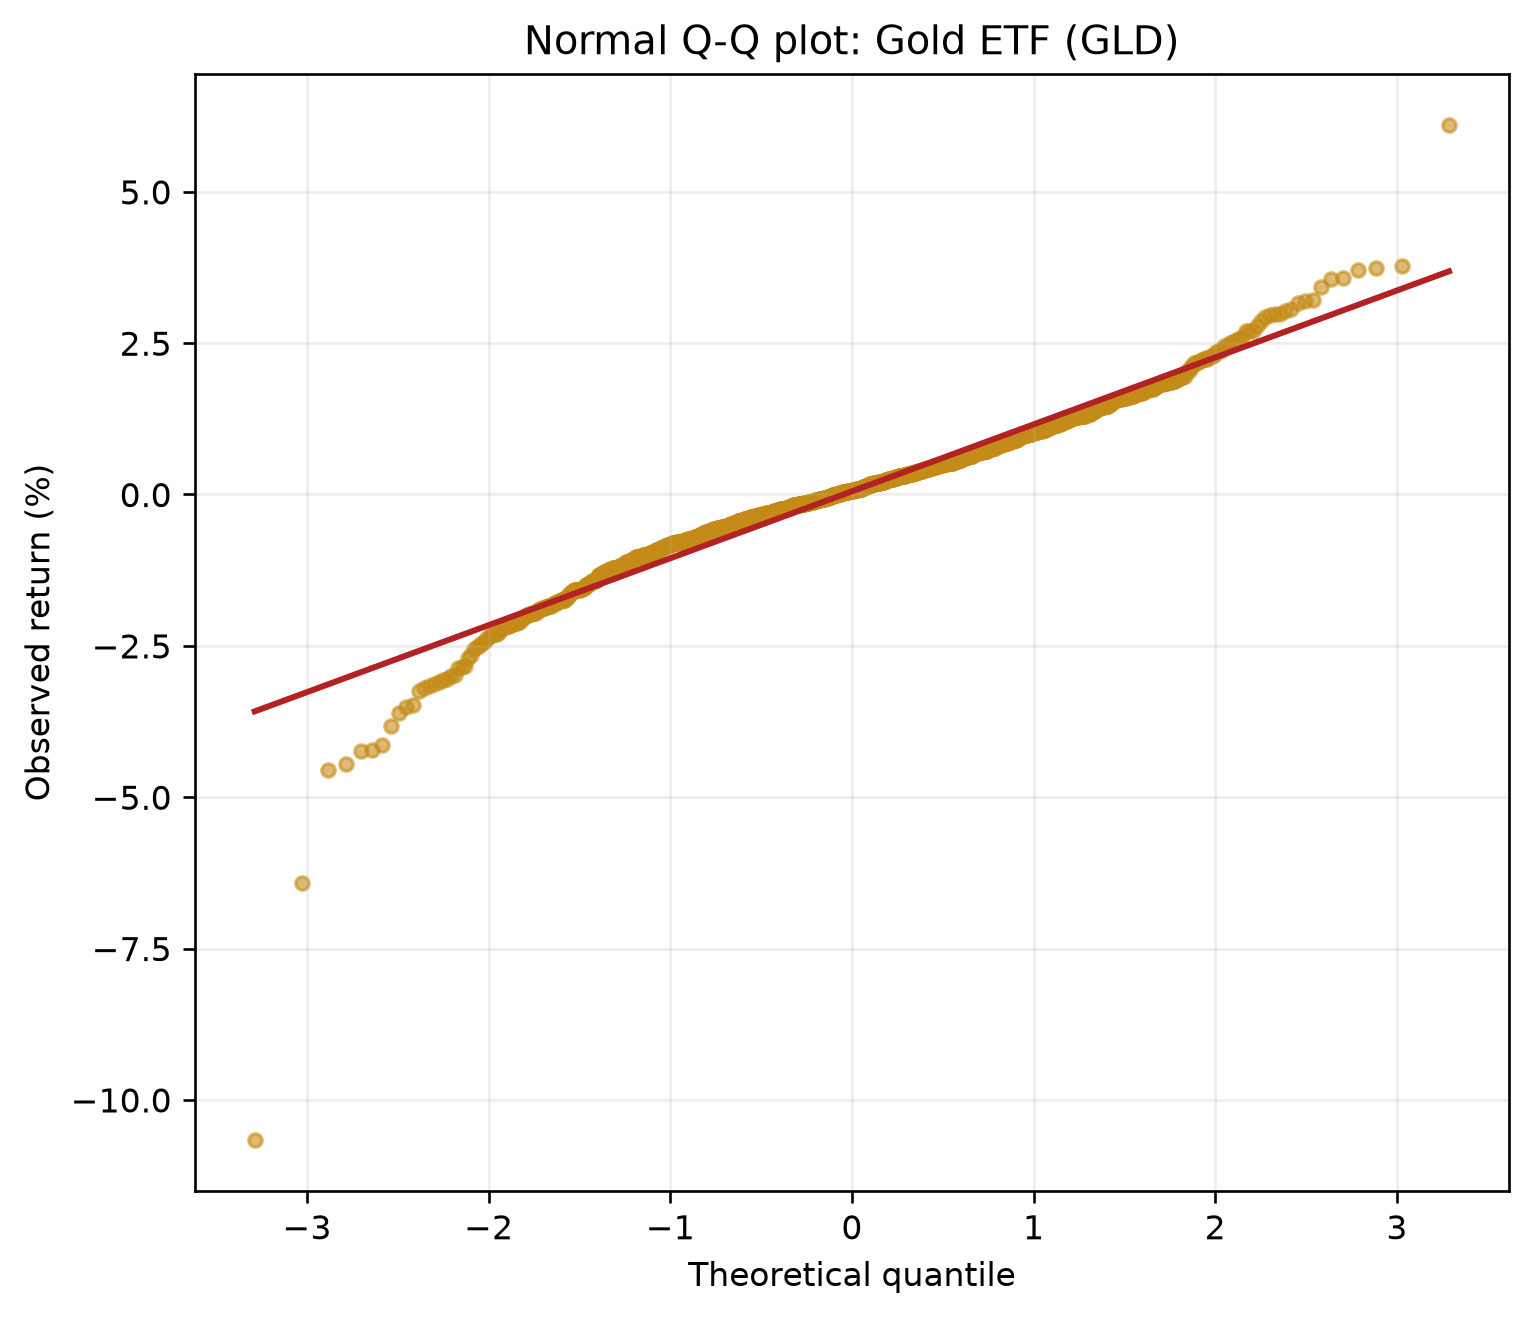
\includegraphics[width=\linewidth]{img/team7_empirical/qqplot_normal_gold.png}
\end{minipage}\hfill
\begin{minipage}{0.49\textwidth}
\centering
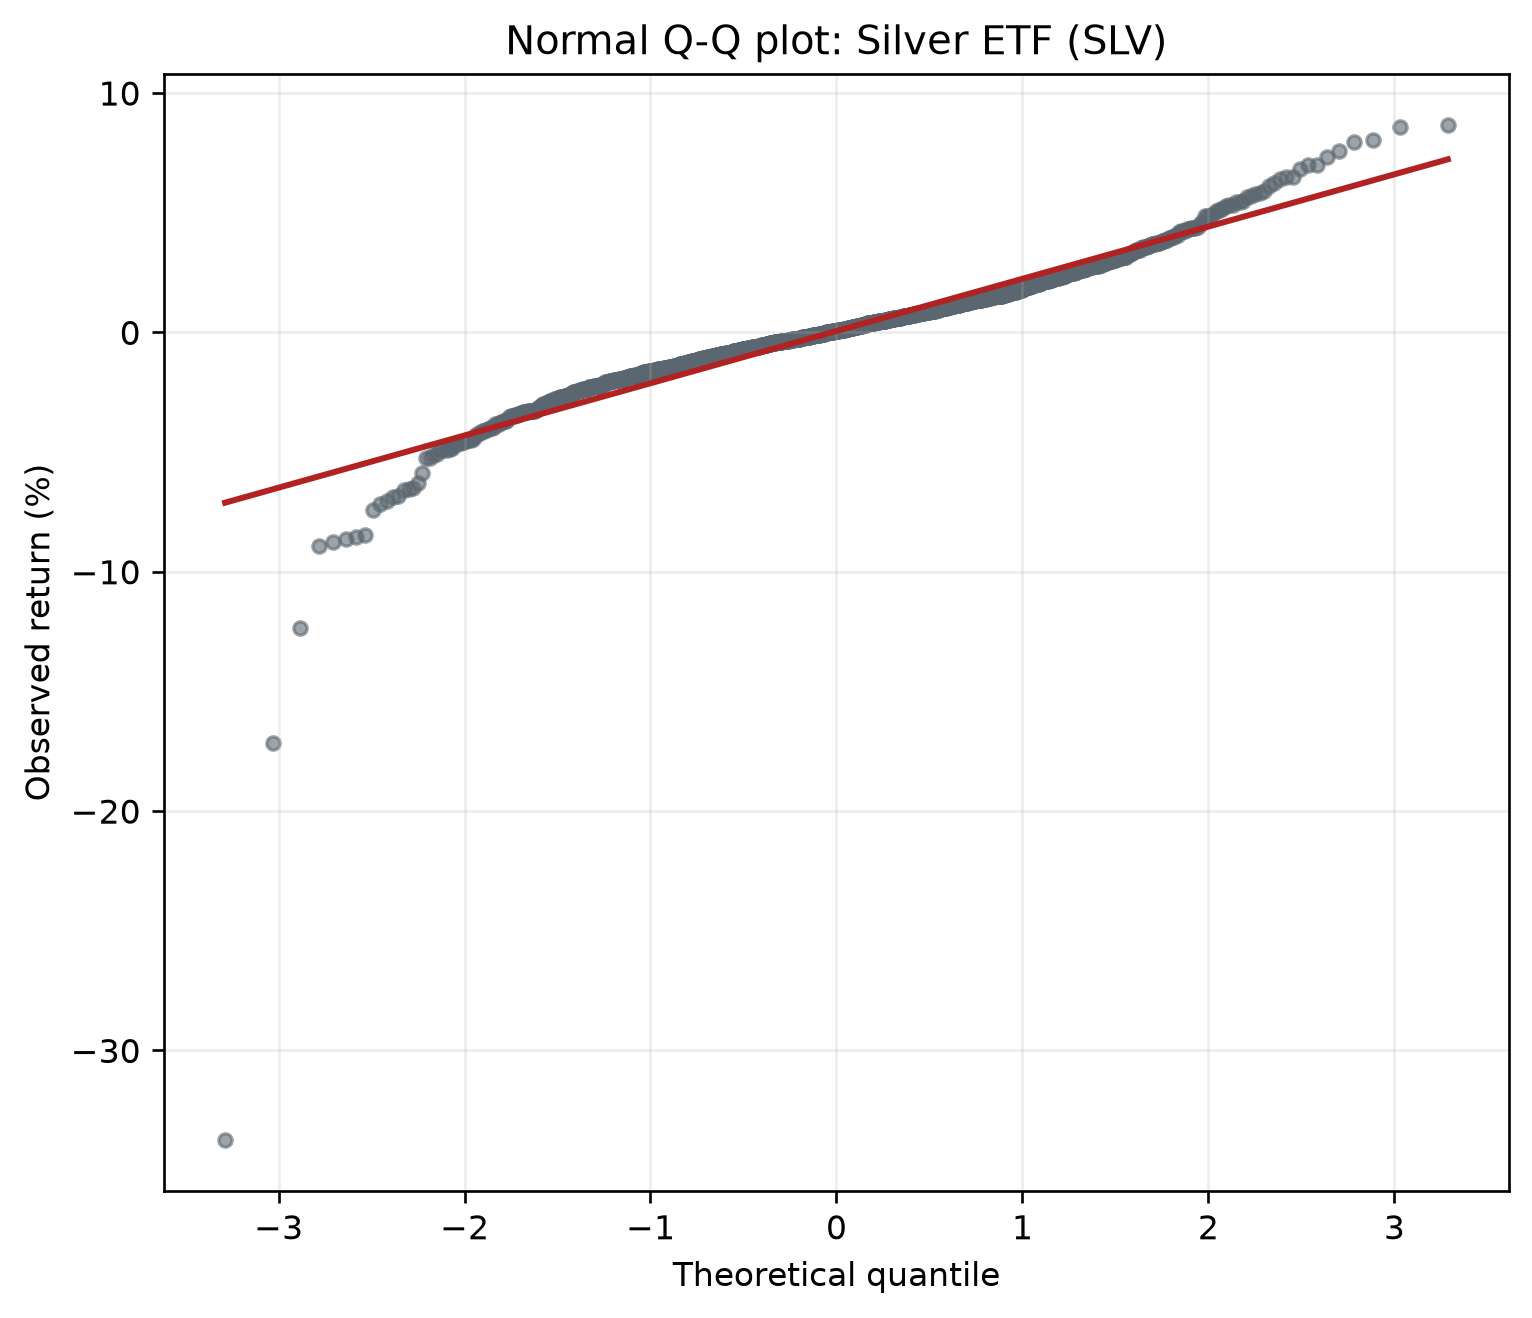
\includegraphics[width=\linewidth]{img/team7_empirical/qqplot_normal_silver.png}
\end{minipage}
\caption{Current LSE normal Q--Q diagnostics for GLD and SLV returns}
\label{fig:t7-return-qqplots}
\end{figure}

Absolute and squared returns show positive serial dependence even when raw
return autocorrelation is weak. Large changes tend to be followed by large
changes of either sign, and shocks decay slowly. This volatility clustering is
the empirical feature that a constant-variance mean model misses most clearly.

\begin{figure}[htbp]
\centering
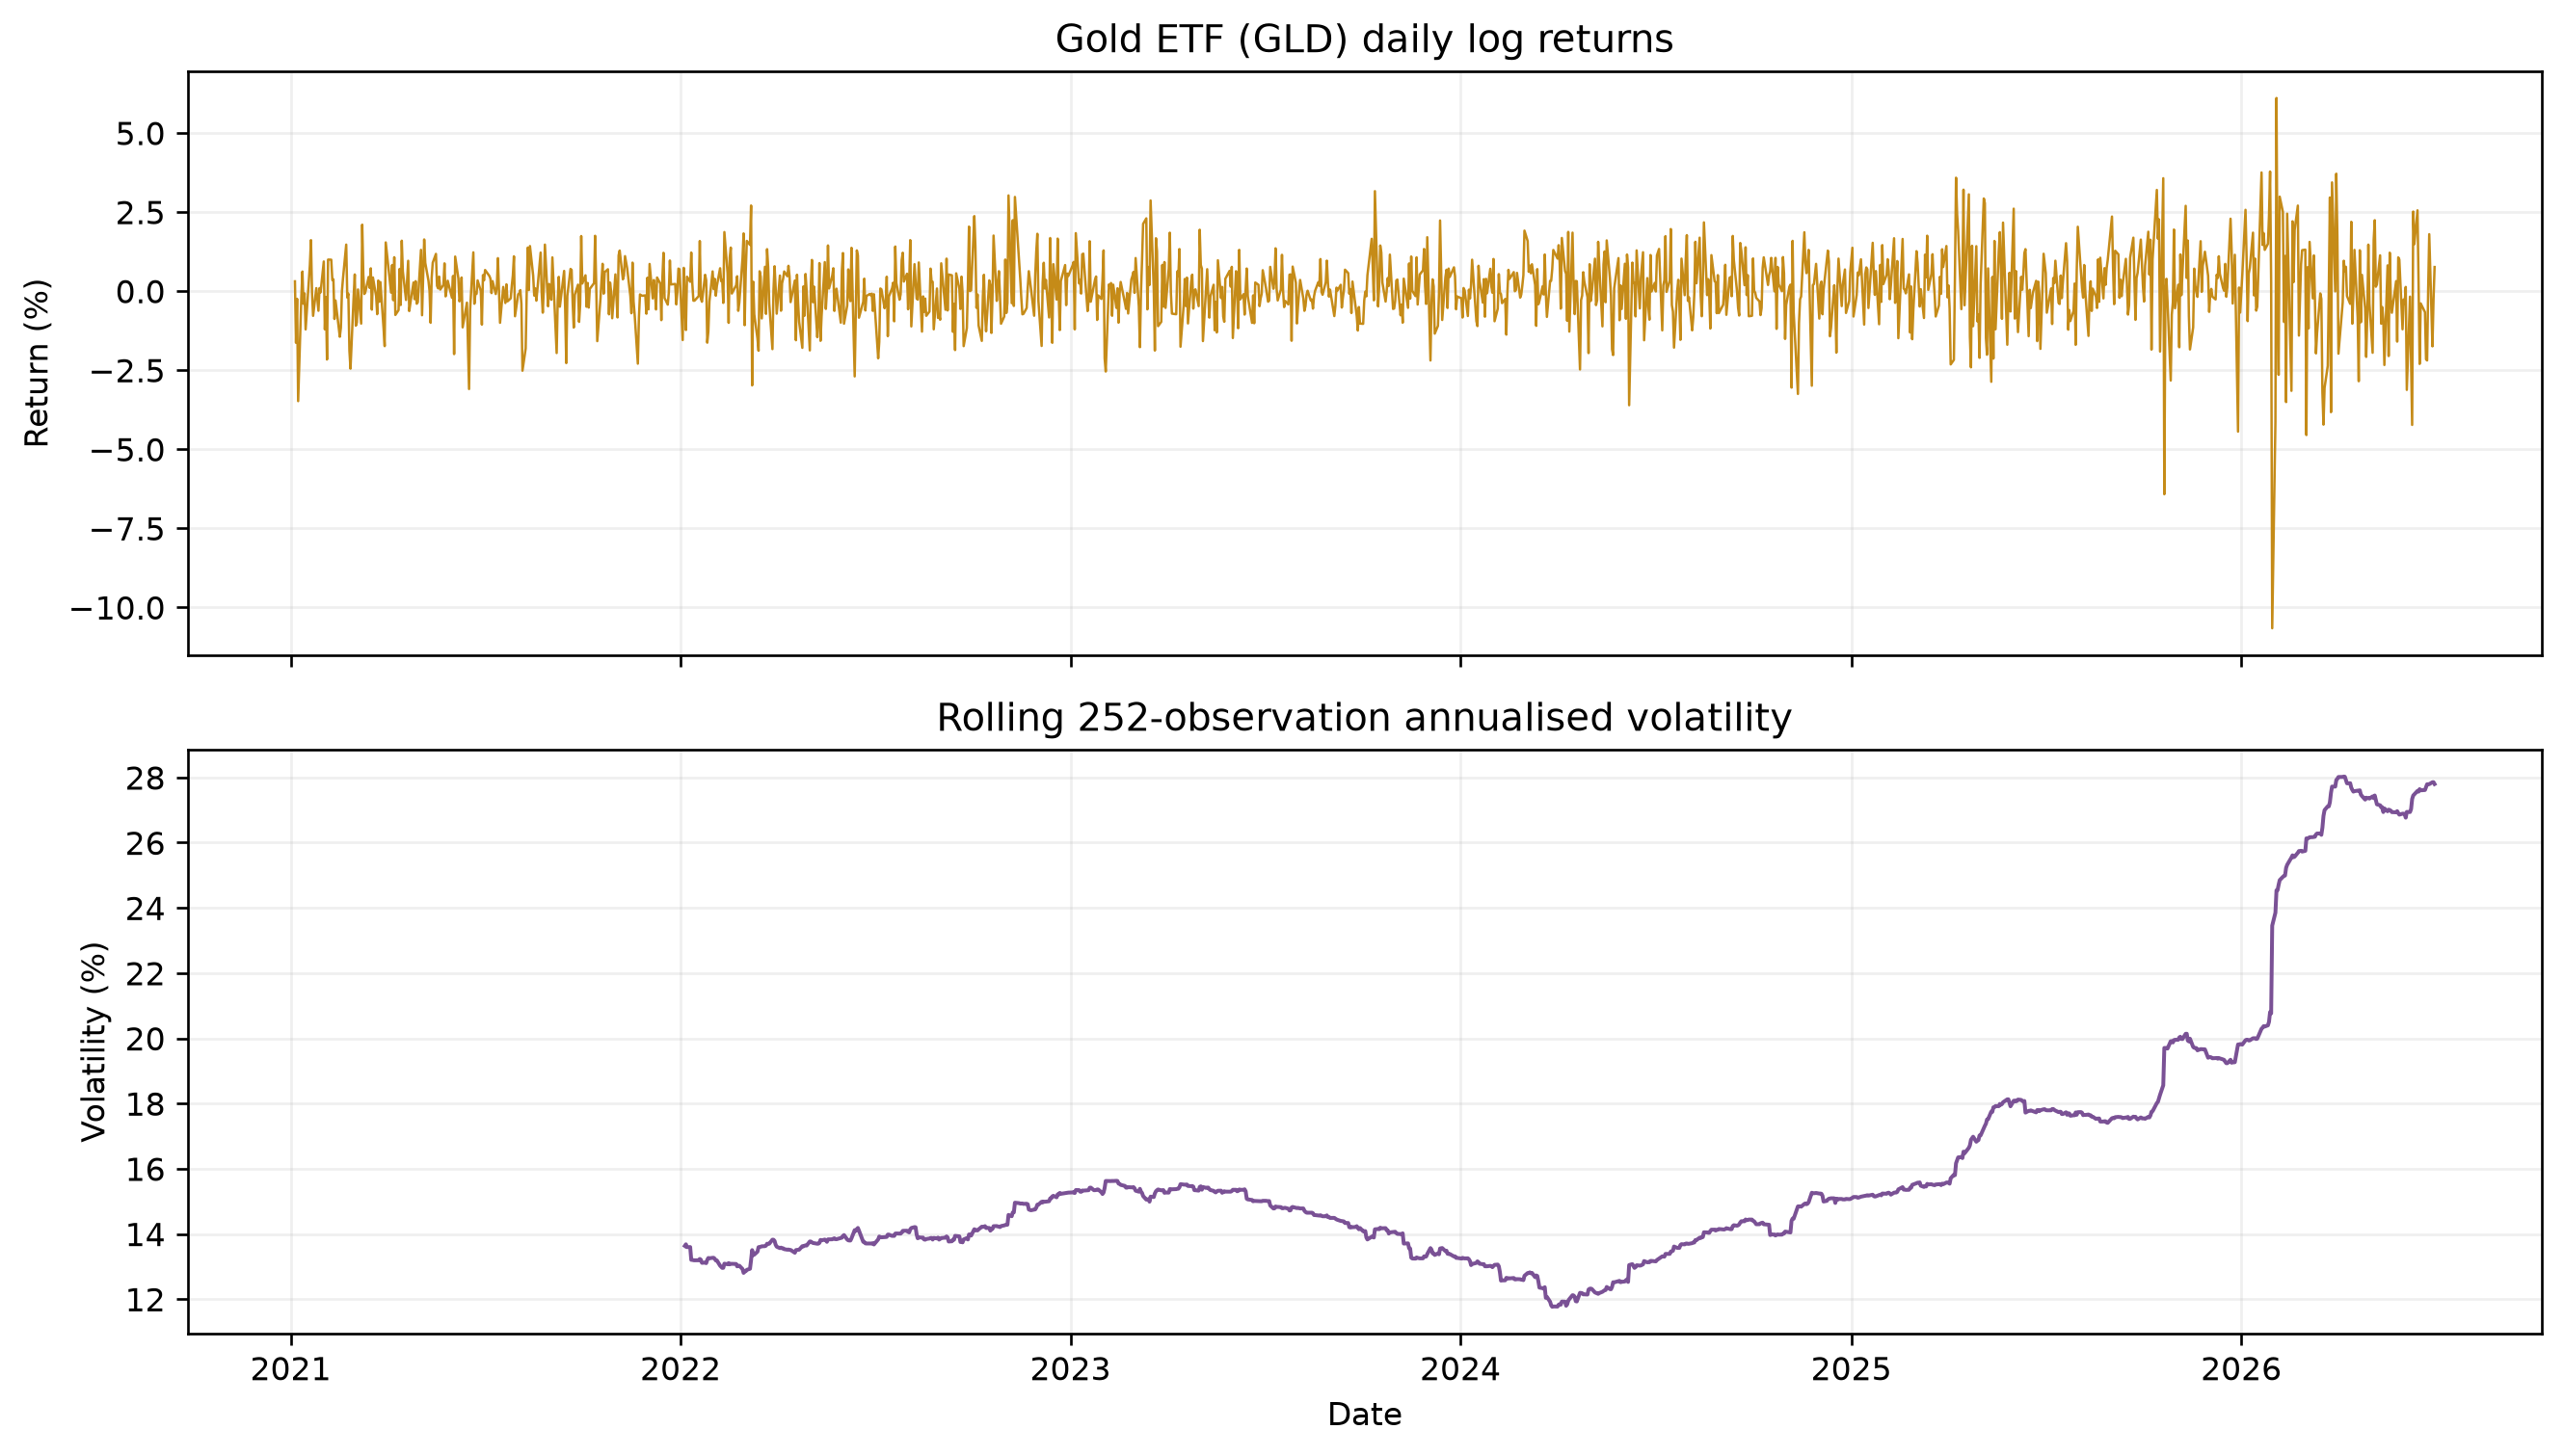
\includegraphics[width=0.88\textwidth]{img/team7_empirical/returns_rollingvol_gold.png}
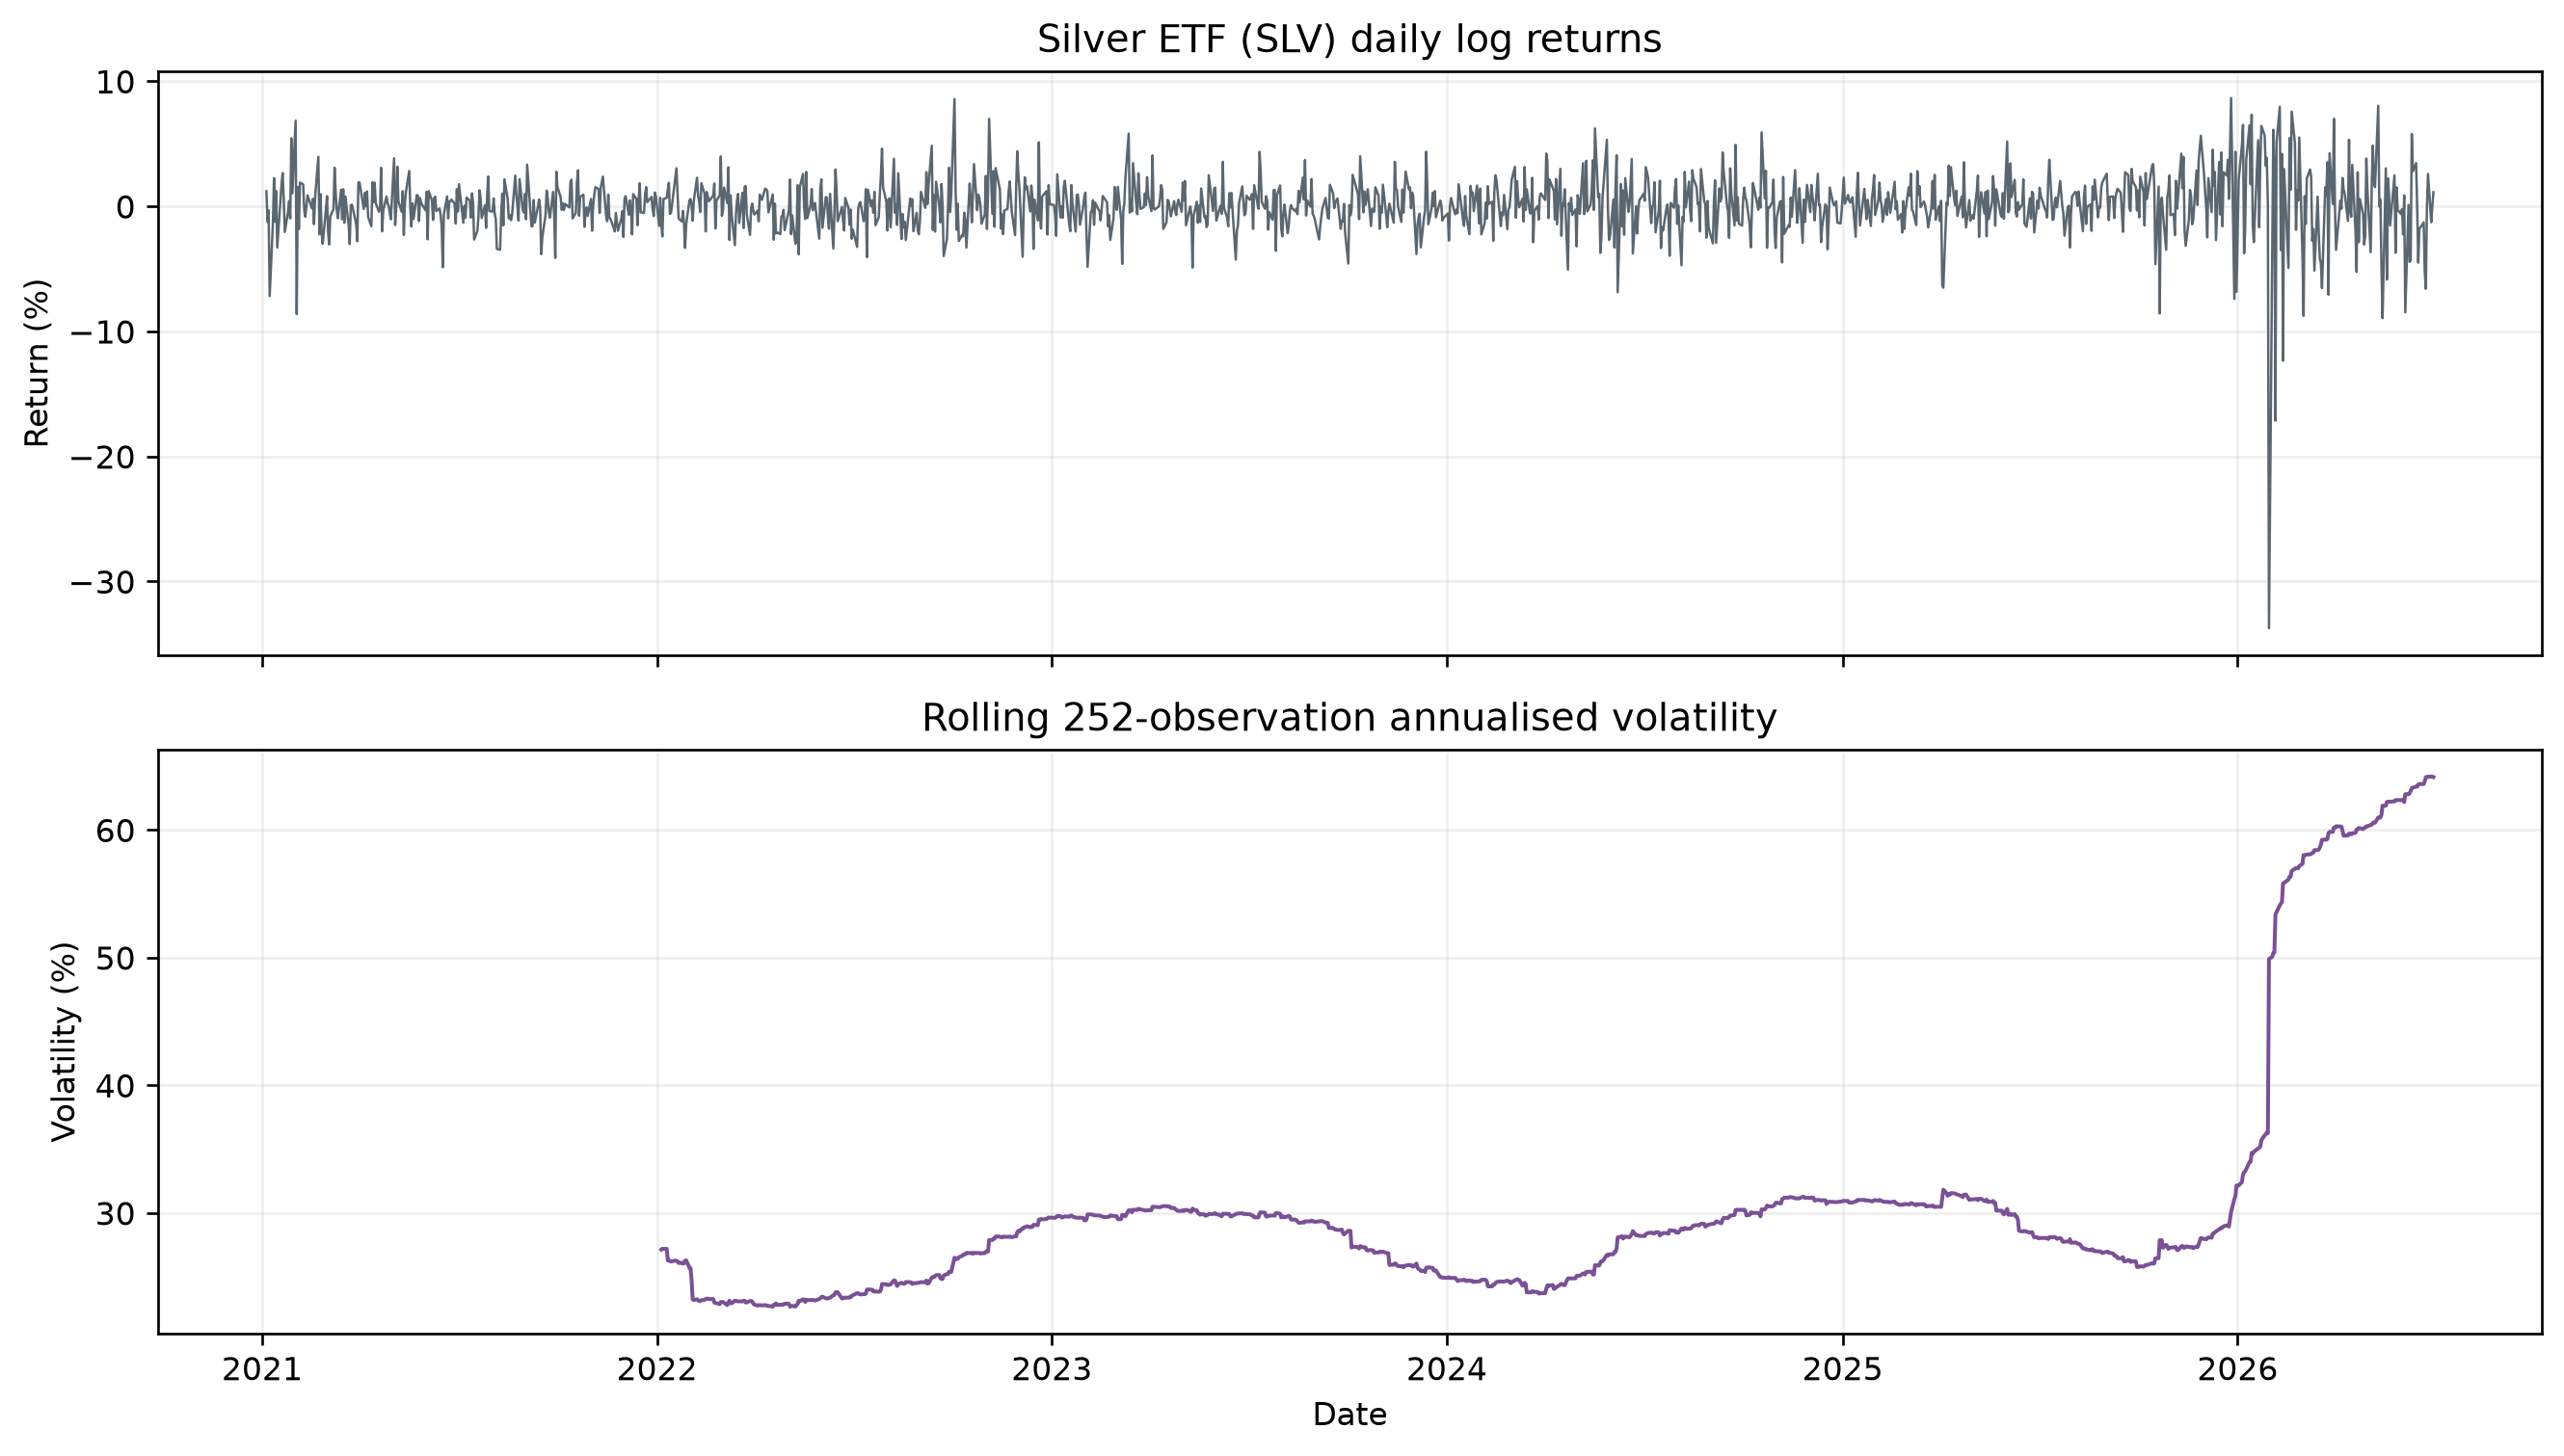
\includegraphics[width=0.88\textwidth]{img/team7_empirical/returns_rollingvol_silver.png}
\caption{Current LSE daily returns and rolling 252-observation annualized volatility for GLD and SLV}
\label{fig:t7-rolling-volatility}
\end{figure}

The ACF panels in Figure~\ref{fig:t7-acf-grid} separate the mean and variance
signals. Raw-return autocorrelations remain close to zero, whereas absolute
and squared returns retain positive dependence over many lags. The compact
persistence statistics in Table~\ref{tab:t7-persistence} reach the same
conclusion.

\begin{figure}[htbp]
\centering
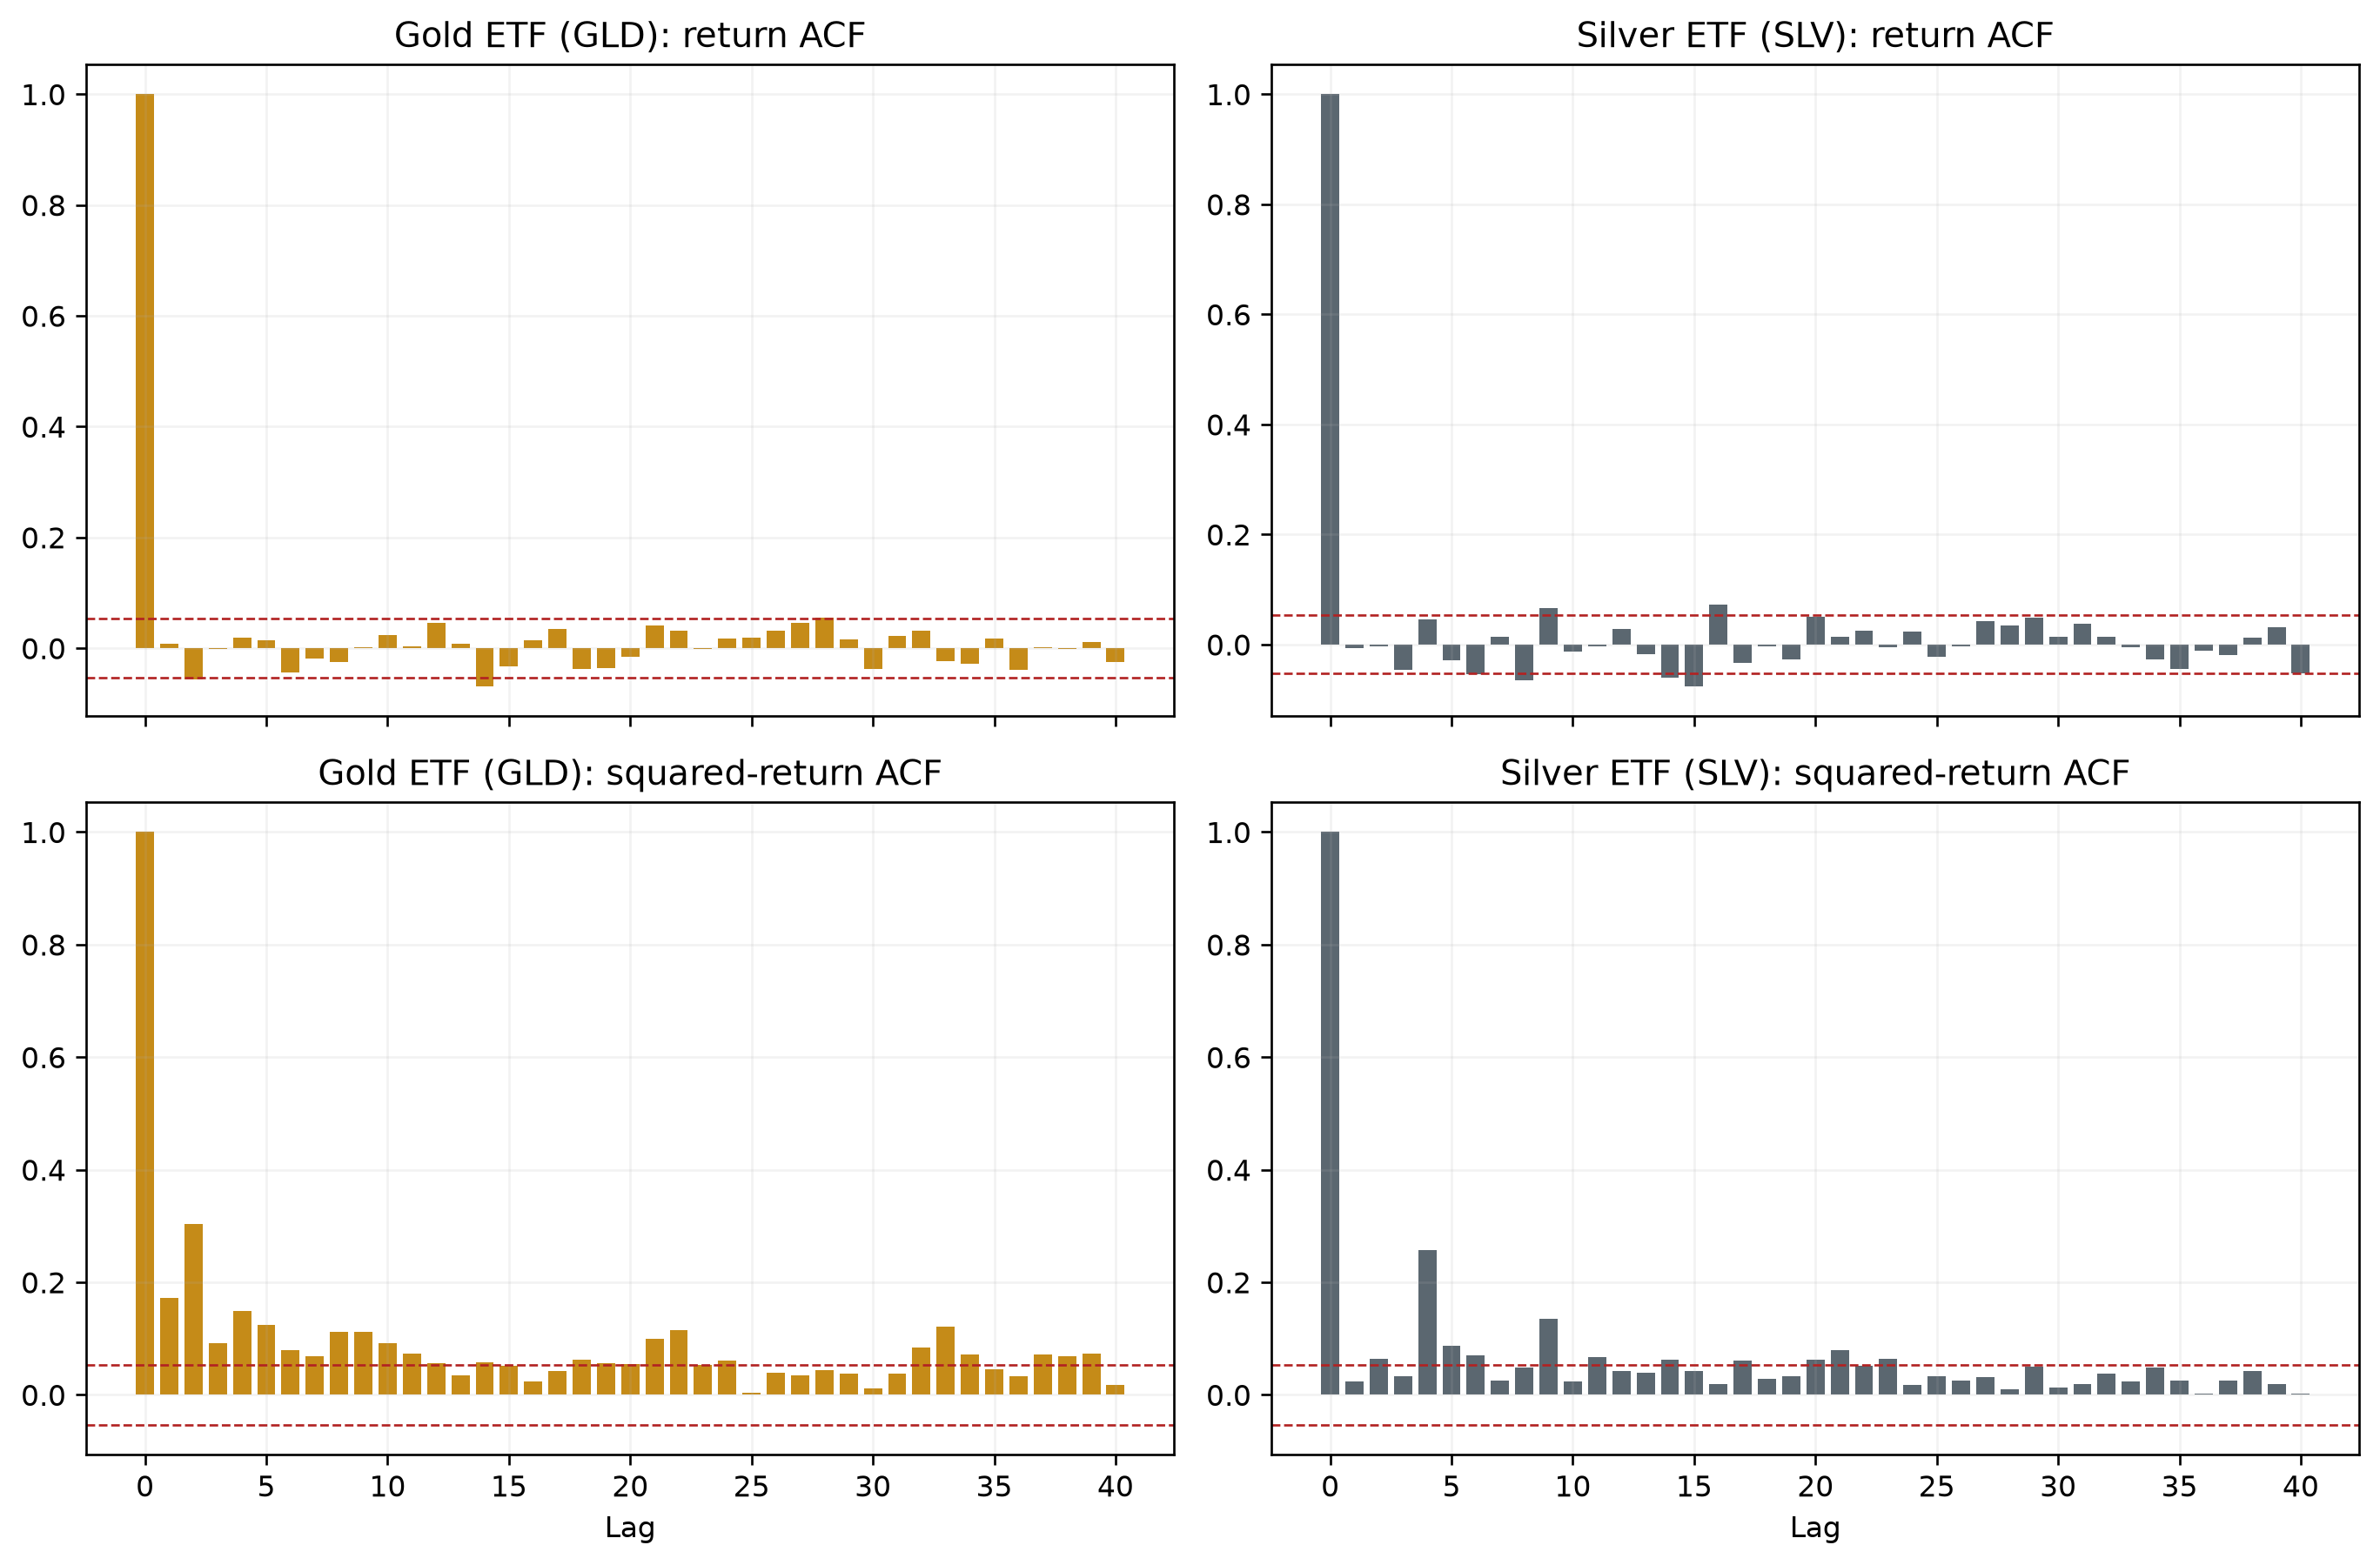
\includegraphics[width=0.95\textwidth]{img/team7_empirical/acf_grid_gold_silver.png}
\caption{Current LSE autocorrelation diagnostics for GLD/SLV returns and squared returns}
\label{fig:t7-acf-grid}
\end{figure}

\begin{table}[htbp]
\centering
\caption{Short-run volatility-persistence diagnostics}
\label{tab:t7-persistence}
\small
\begin{tabular}{lrrr}
\toprule
Asset & $\hat\phi$ & Robust s.e. & $t$-statistic \\
\midrule
Gold   & 0.115 & 0.020 & 5.60 \\
Silver & 0.156 & 0.024 & 6.40 \\
\bottomrule
\end{tabular}
\begin{minipage}{0.94\textwidth}
\footnotesize\emph{Notes:} OLS estimates from
$|r_t|=c+\phi|r_{t-1}|+\varepsilon_t$, with HC1 standard errors. Values
reproduce the compact persistence table in the Team~7 article.
\end{minipage}
\end{table}

\section{ARCH and GARCH Evidence}

An ARCH model makes conditional variance depend on past squared innovations,
while a GARCH model also propagates its own lagged variance. For the benchmark
GARCH$(1,1)$,
\[
 r_t=\mu+\varepsilon_t,\qquad
 \sigma_t^2=\omega+\alpha\varepsilon_{t-1}^2+\beta\sigma_{t-1}^2.
\]
The unified branch fits a Gaussian GARCH$(1,1)$ directly to the current LSE
returns. The estimates are
$(\hat\omega,\hat\alpha,\hat\beta)\approx(0.05385,0.10894,0.84798)$ for GLD and
$(0.04080,0.05453,0.93900)$ for SLV when returns are expressed in percentage
points. Both optimizers converge and $\hat\alpha+\hat\beta<1$; persistence is
especially high for SLV.

\begin{table}[htbp]
\centering
\caption{GARCH(1,1) estimates for gold and silver daily returns}
\label{tab:t7-garch-parameters}
\small
\resizebox{0.96\textwidth}{!}{%
\begin{tabular}{lrrrrrr}
\toprule
Asset & $\hat\mu$ & $\hat\omega$ & $\hat\alpha$ & $\hat\beta$
& $\hat\alpha+\hat\beta$ & $\hat\sigma^2_{\infty}$ \\
\midrule
GLD & 0.03494 & 0.05385 & 0.10894 & 0.84798 & 0.95692 & 1.2500 \\
SLV & 0.01495 & 0.04080 & 0.05453 & 0.93900 & 0.99353 & 6.3067 \\
\bottomrule
\end{tabular}}
\begin{minipage}{0.94\textwidth}
\footnotesize\emph{Notes:} Returns and conditional volatilities are expressed
in percentage units. When $\hat\alpha+\hat\beta<1$,
$\hat\sigma^2_{\infty}=\hat\omega/(1-\hat\alpha-\hat\beta)$.
\end{minipage}
\end{table}

Figure~\ref{fig:t7-garch-conditional-volatility} shows the regenerated fitted
conditional-volatility paths. Silver fluctuates around a higher baseline and
has larger spikes; for both metals the decay after stress episodes is gradual,
as implied by the near-unit persistence estimates.

\begin{figure}[htbp]
\centering
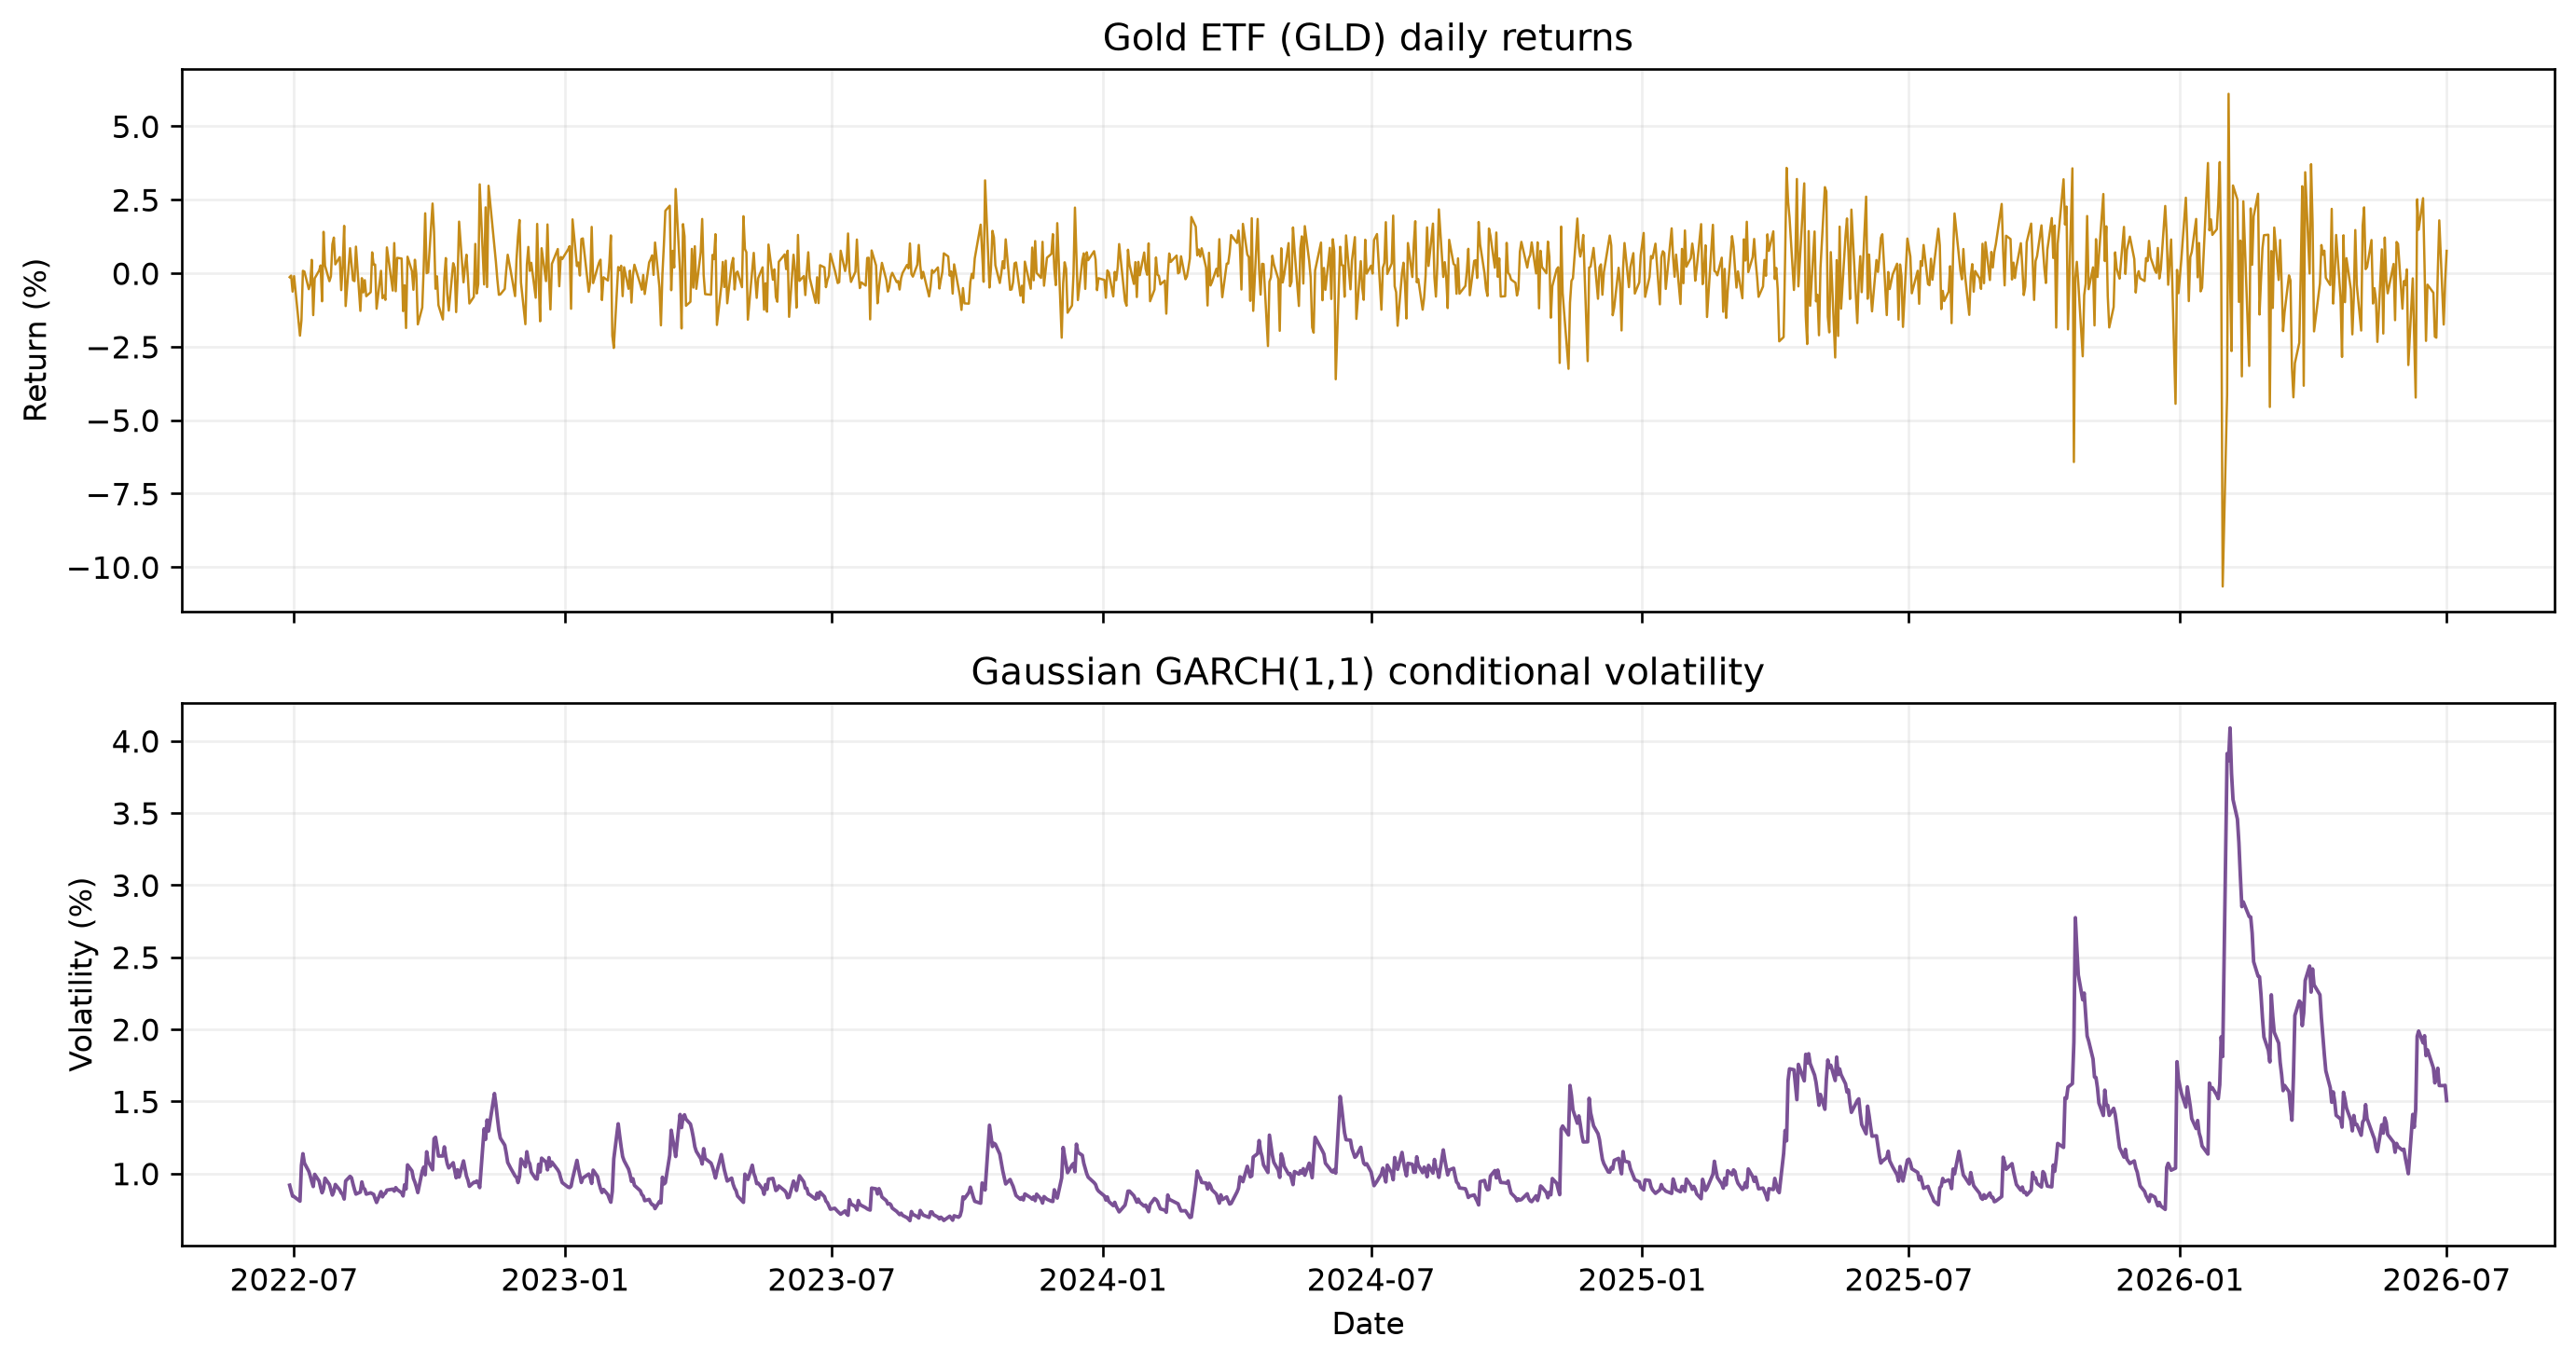
\includegraphics[width=0.90\textwidth]{img/team7_empirical/garch_condvol_gold.png}
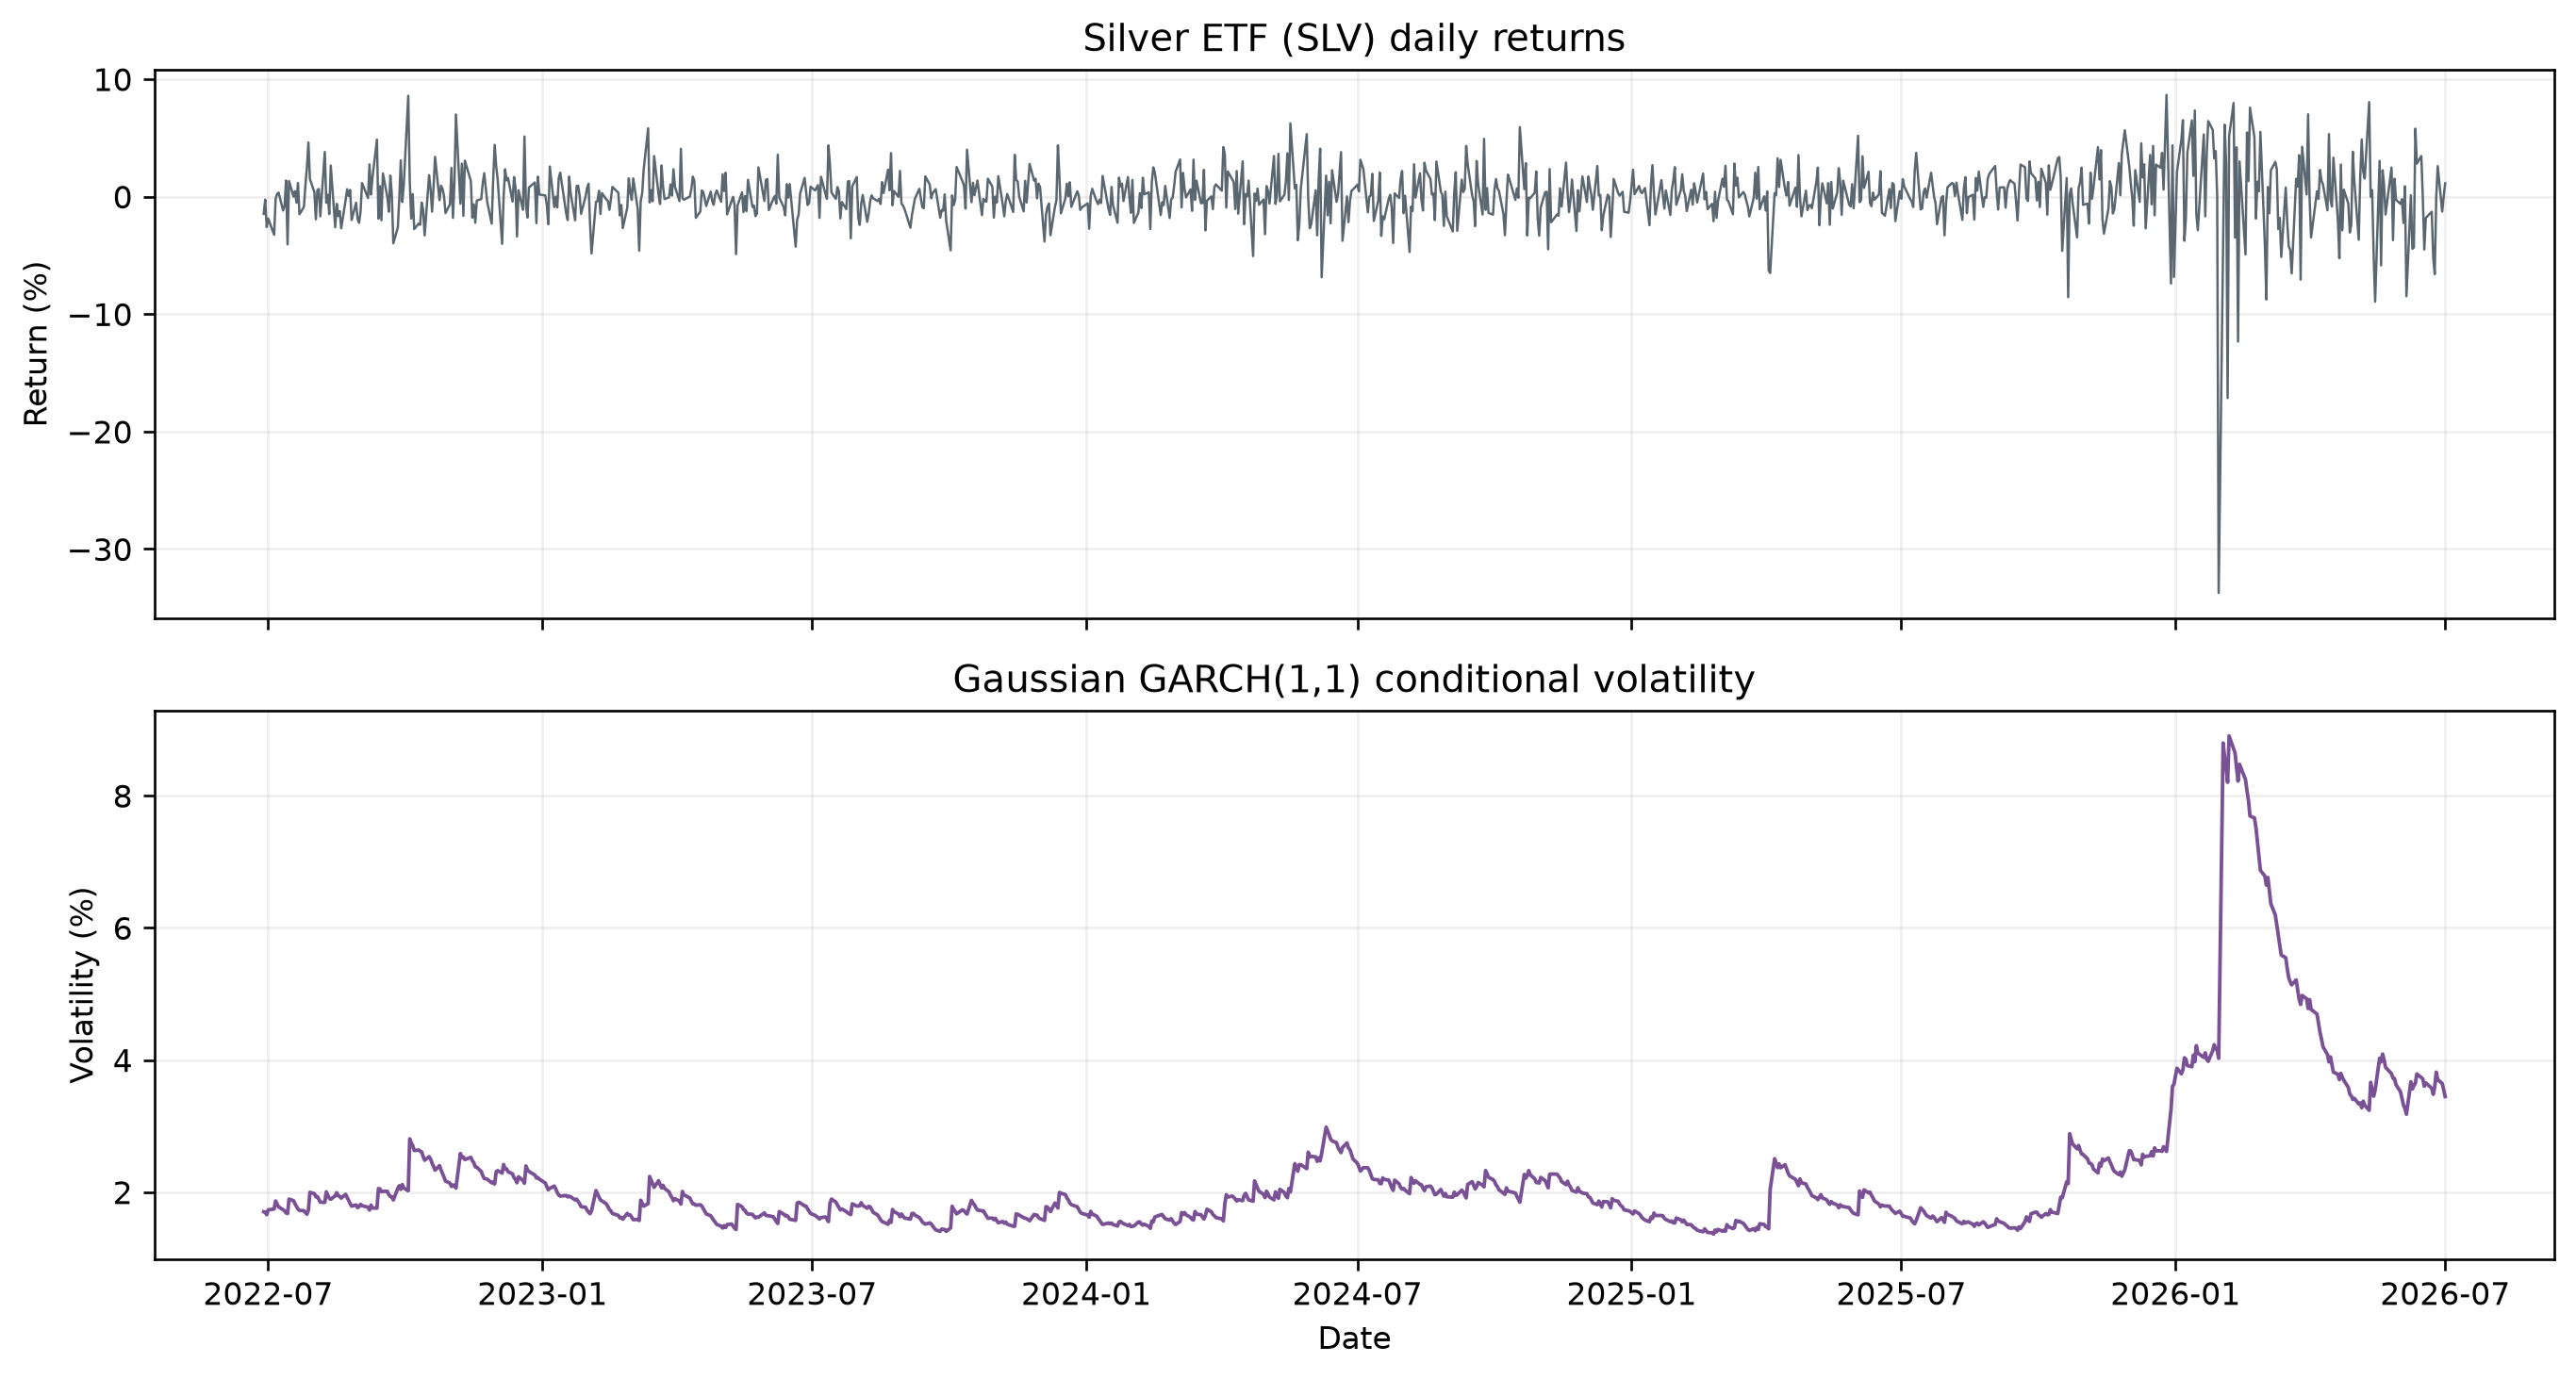
\includegraphics[width=0.90\textwidth]{img/team7_empirical/garch_condvol_silver.png}
\caption{Current LSE Gaussian GARCH(1,1) conditional volatility for GLD and SLV}
\label{fig:t7-garch-conditional-volatility}
\end{figure}

For historical comparison, the frozen Team~7 end-of-sample variance forecasts in
Table~\ref{tab:t7-garch-forecasts} show the same slow mean reversion. In that legacy run, gold
moves from approximately $0.981$ to $1.002$ squared percentage points over ten
days, toward a long-run level of $1.211$; silver moves from $2.686$ to $2.791$,
toward $4.235$.

\begin{table}[htbp]
\centering
\caption{Frozen Team~7 end-of-sample GARCH conditional-variance forecasts}
\label{tab:t7-garch-forecasts}
\small
\begin{tabular}{crr@{\qquad}crr}
\toprule
$h$ & Gold & Silver & $h$ & Gold & Silver \\
\midrule
1 & 0.981250 & 2.685694 &  6 & 0.993096 & 2.745300 \\
2 & 0.983669 & 2.697803 &  7 & 0.995391 & 2.756943 \\
3 & 0.986064 & 2.709817 &  8 & 0.997662 & 2.768495 \\
4 & 0.988433 & 2.721737 &  9 & 0.999908 & 2.779957 \\
5 & 0.990777 & 2.733565 & 10 & 1.002131 & 2.791329 \\
\bottomrule
\end{tabular}
\begin{minipage}{0.90\textwidth}
\footnotesize\emph{Notes:} Forecast horizon $h$ is measured in trading days;
variances are in squared percentage-return units.
\end{minipage}
\end{table}

These estimates show why GARCH is useful: it converts clustering into a
dynamic conditional-variance forecast. GARCH remains a discrete-time model,
and this is a strength for empirical diagnosis rather than a conceptual flaw.
Its role here is to show that the relevant predictable object is volatility
more than the daily conditional mean.

\section{Long-Memory Cross-Check: GPH and Fractional Differencing}

GARCH captures short-run clustering with a recursive conditional variance. A
separate question is whether a volatility proxy also displays hyperbolically
decaying, long-range dependence. Team~7 applied the semiparametric
Geweke--Porter--Hudak estimator to absolute daily returns. The frozen published
estimates in Table~\ref{tab:t7-gph} are positive and precisely estimated. The
current LSE figure rebuild estimates $d=0.452$ for GLD and clips the SLV
estimate at the implementation boundary $d=0.490$; it does not reuse the
published point estimates.

\begin{table}[htbp]
\centering
\caption{Frozen Team~7 GPH estimates of the fractional differencing parameter for absolute returns}
\label{tab:t7-gph}
\small
\begin{tabular}{lrrr}
\toprule
Asset & $\hat d$ & s.e.($\hat d$) & $t$-statistic \\
\midrule
Gold   & 0.576 & 0.090 & 6.39 \\
Silver & 0.552 & 0.080 & 6.91 \\
\bottomrule
\end{tabular}
\end{table}

The regenerated visual evidence is consistent with persistent absolute returns. Their
autocorrelations remain positive across many lags in
Figure~\ref{fig:t7-absolute-return-acf}, while fractional filtering visibly
reduces low-frequency persistence in
Figure~\ref{fig:t7-fractional-differencing}.

\begin{figure}[htbp]
\centering
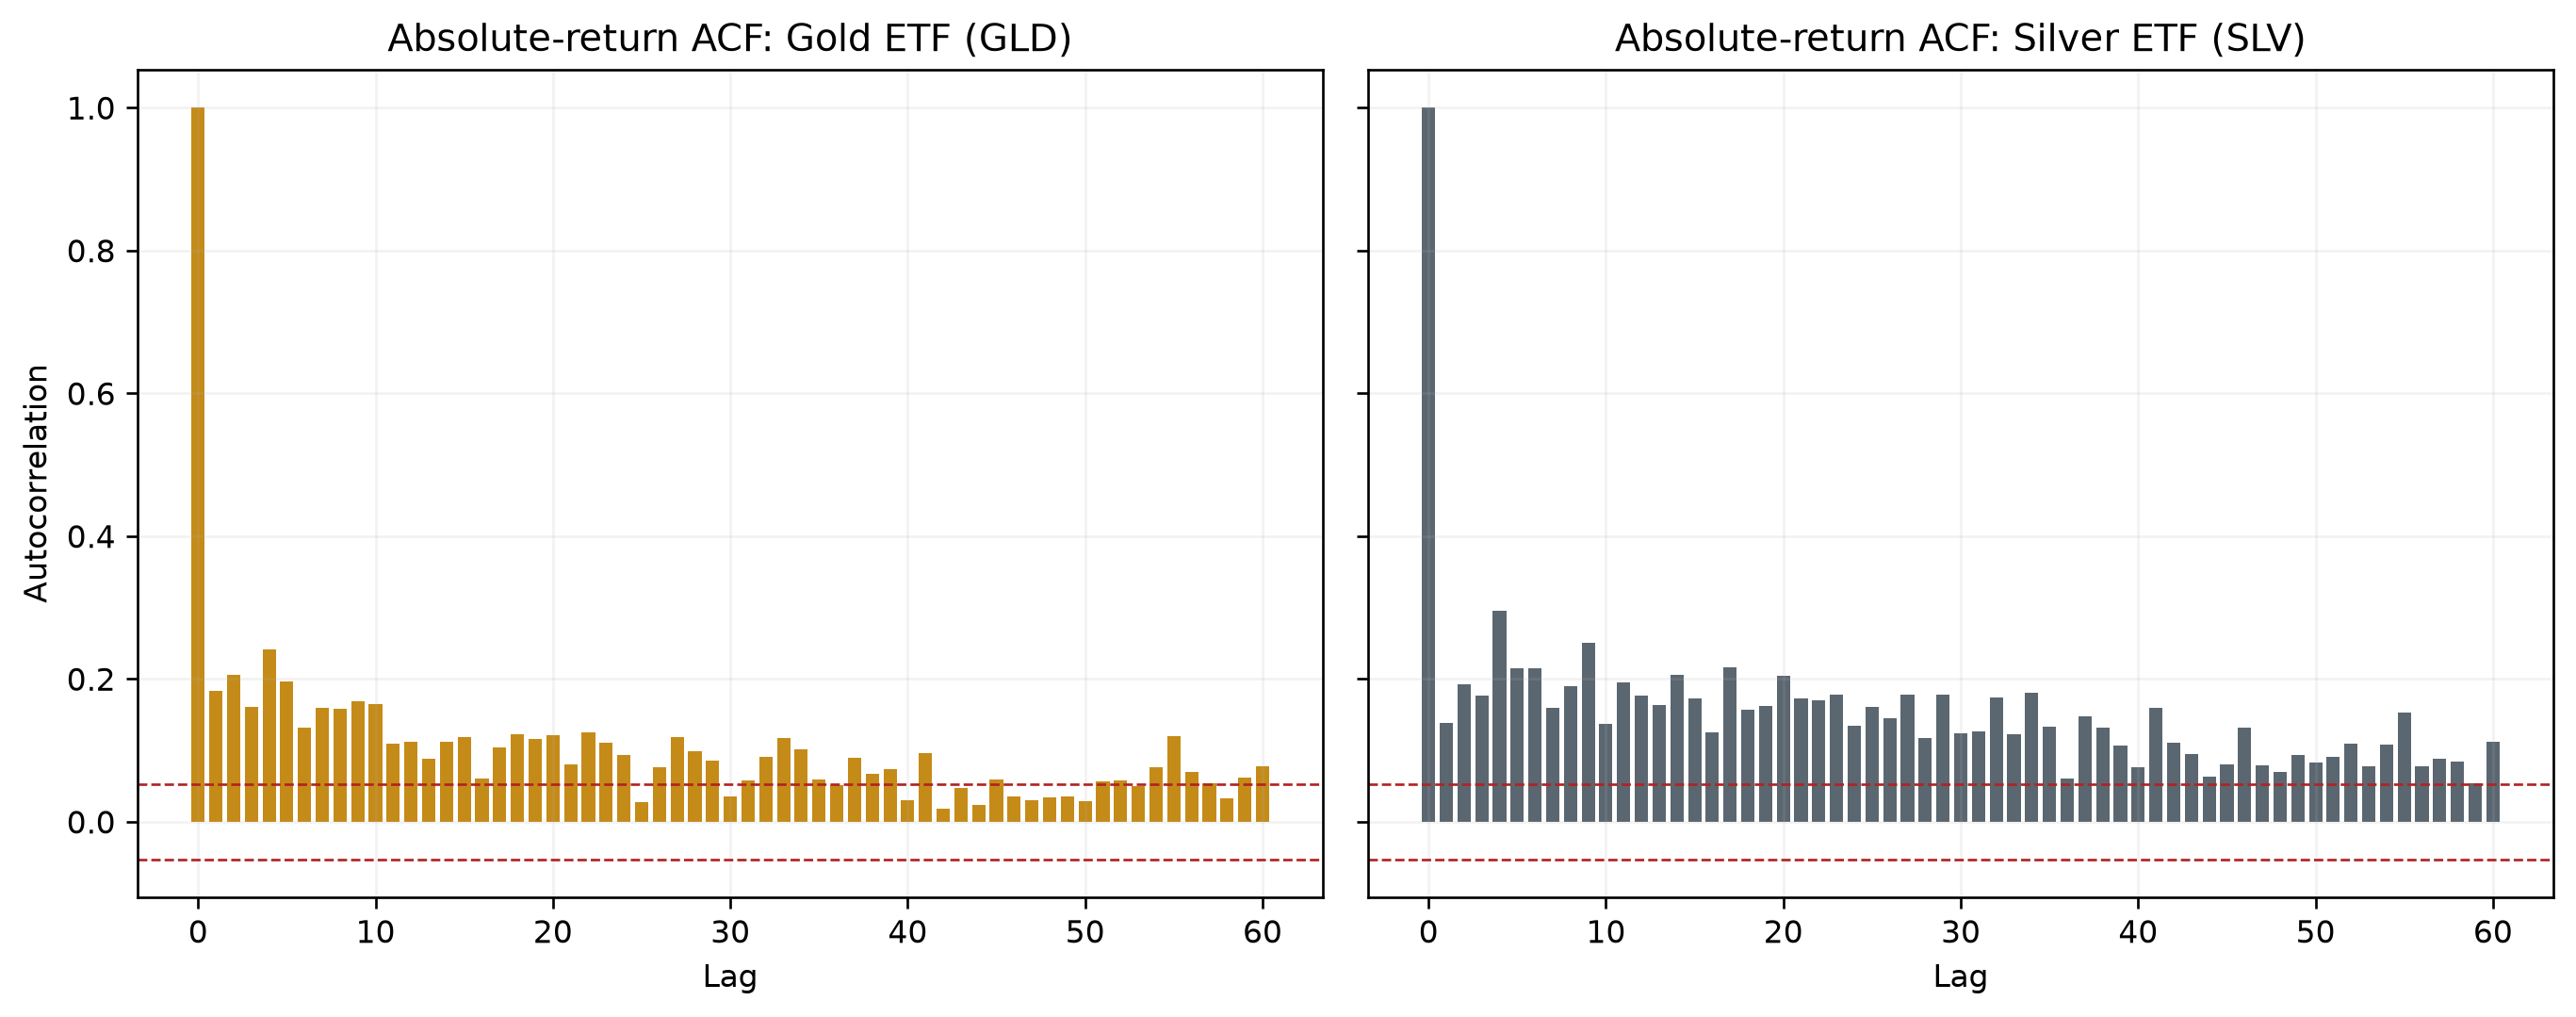
\includegraphics[width=0.88\textwidth]{img/team7_empirical/acf_abs_returns_gold_silver.png}
\caption{Current LSE autocorrelation functions of GLD and SLV absolute returns}
\label{fig:t7-absolute-return-acf}
\end{figure}

\begin{figure}[htbp]
\centering
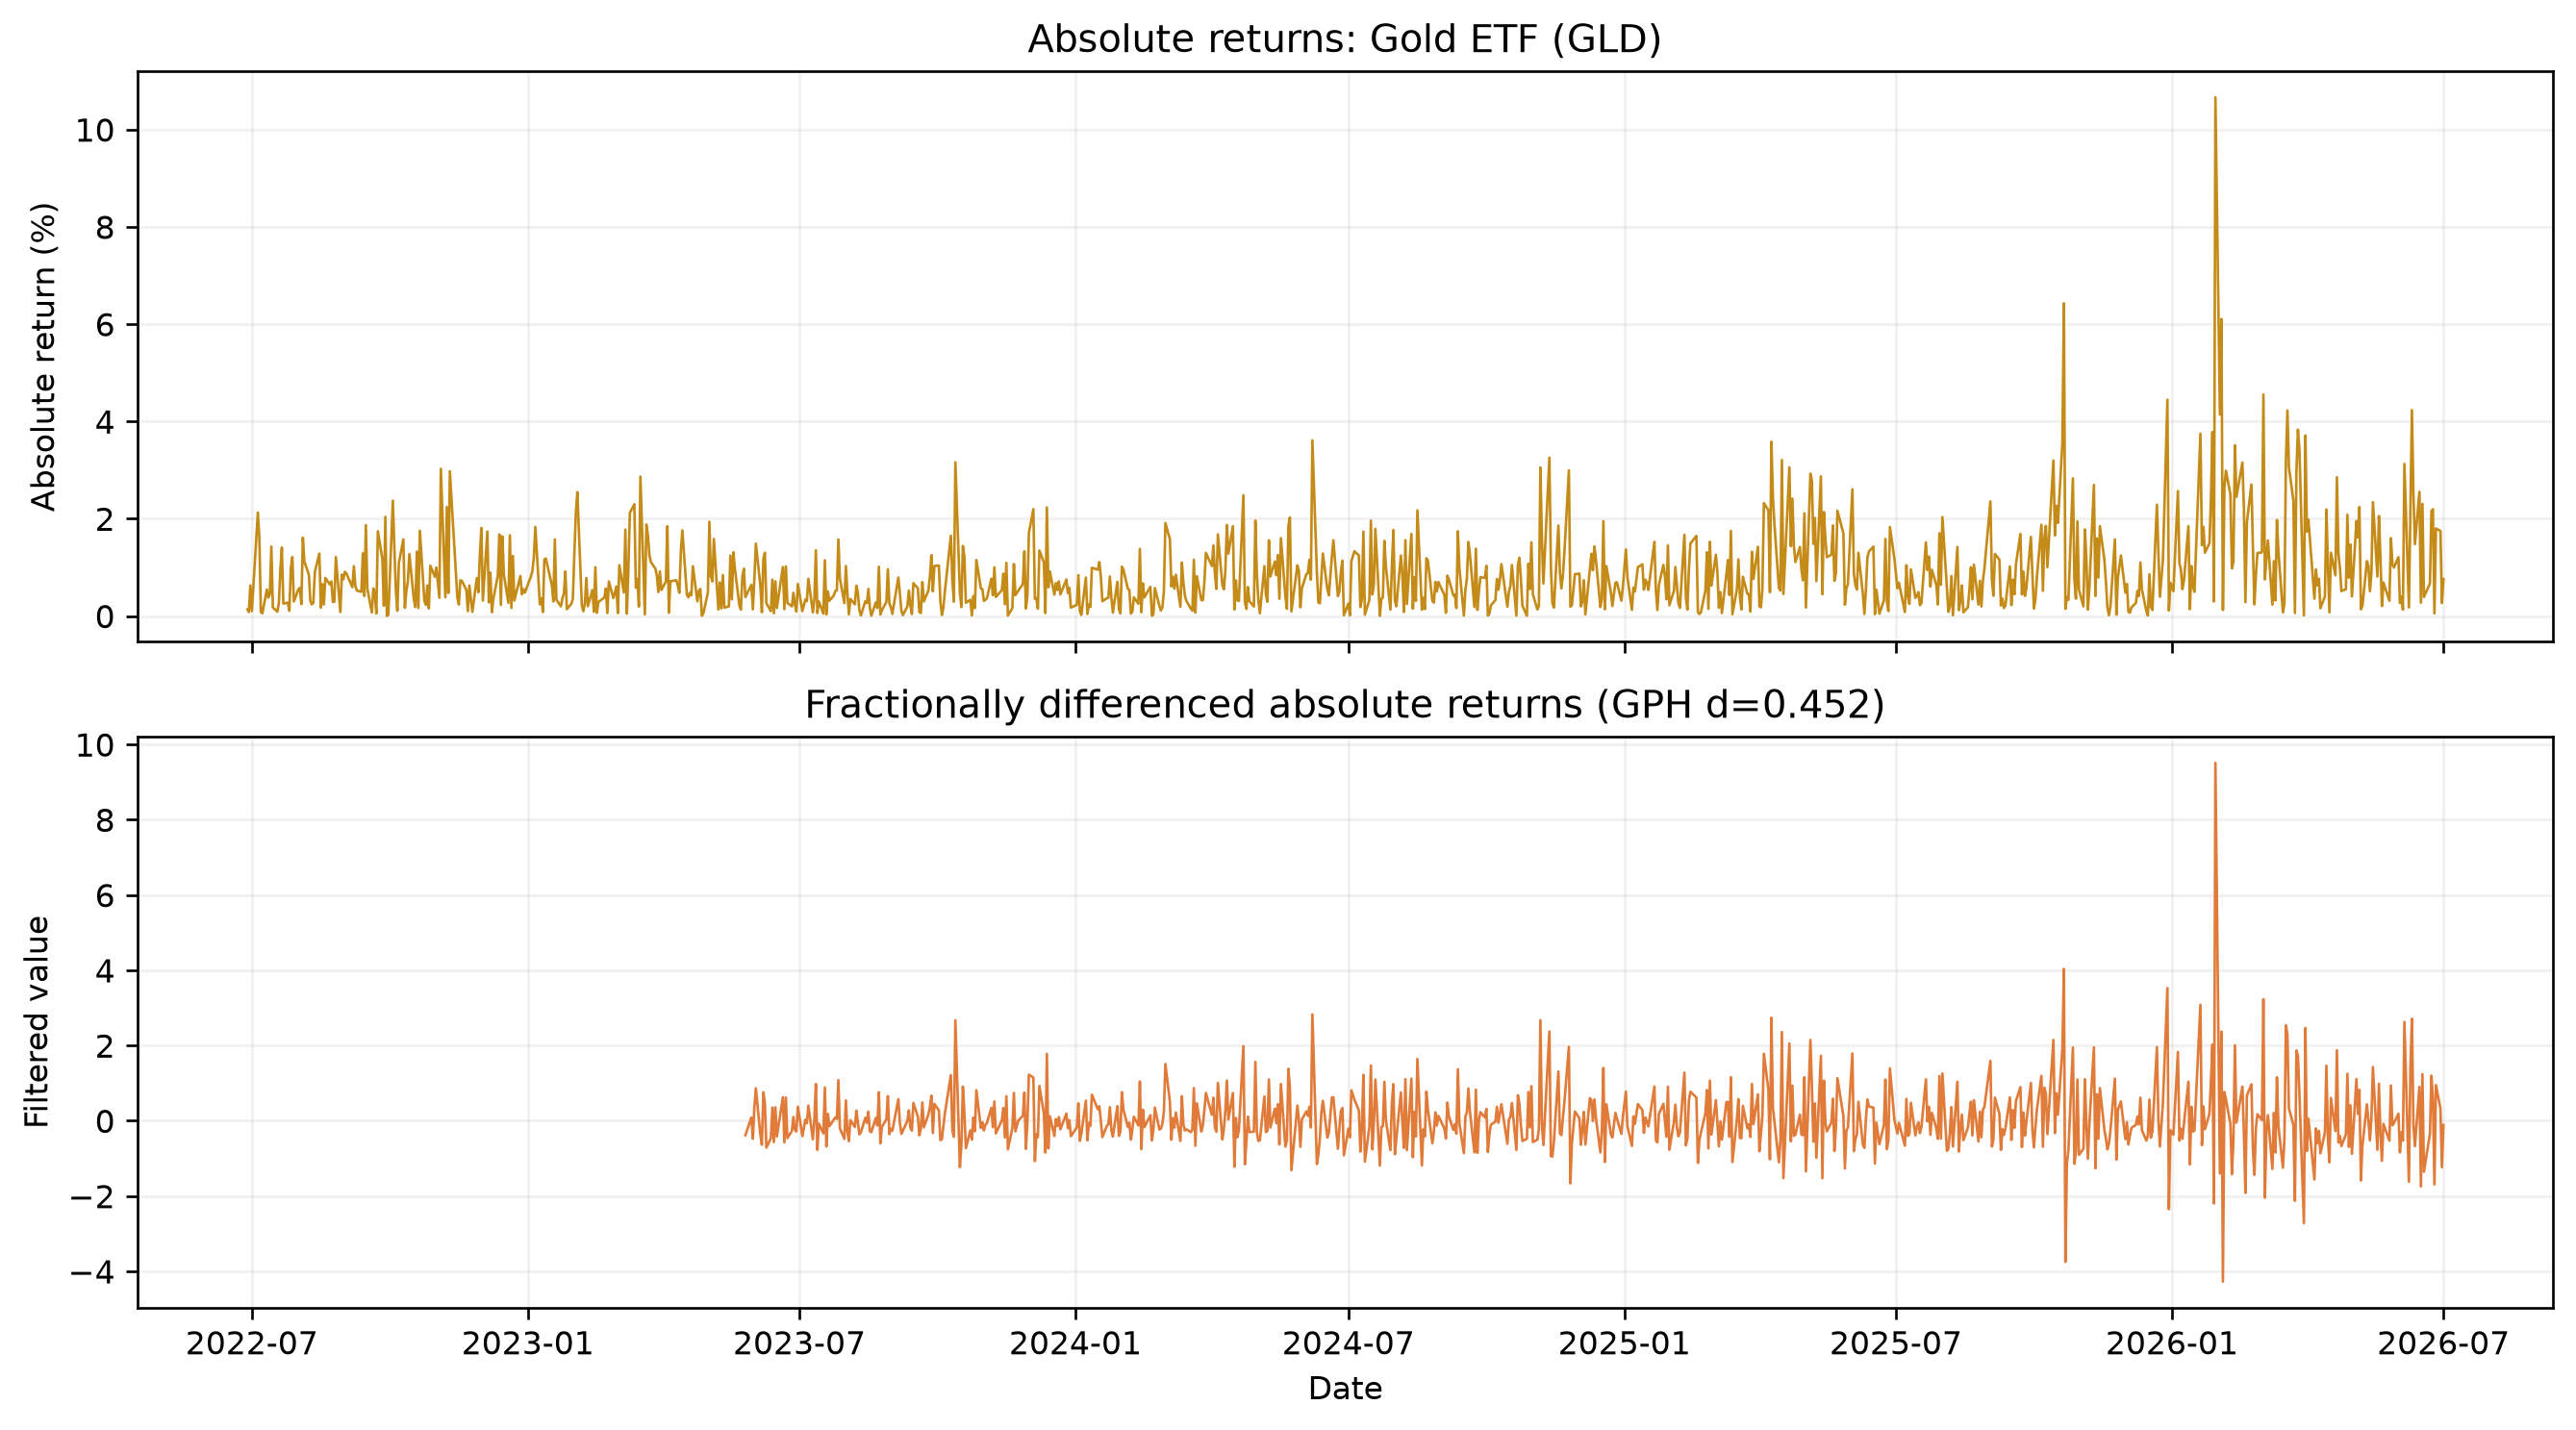
\includegraphics[width=0.86\textwidth]{img/team7_empirical/arfima_fd_gold.png}
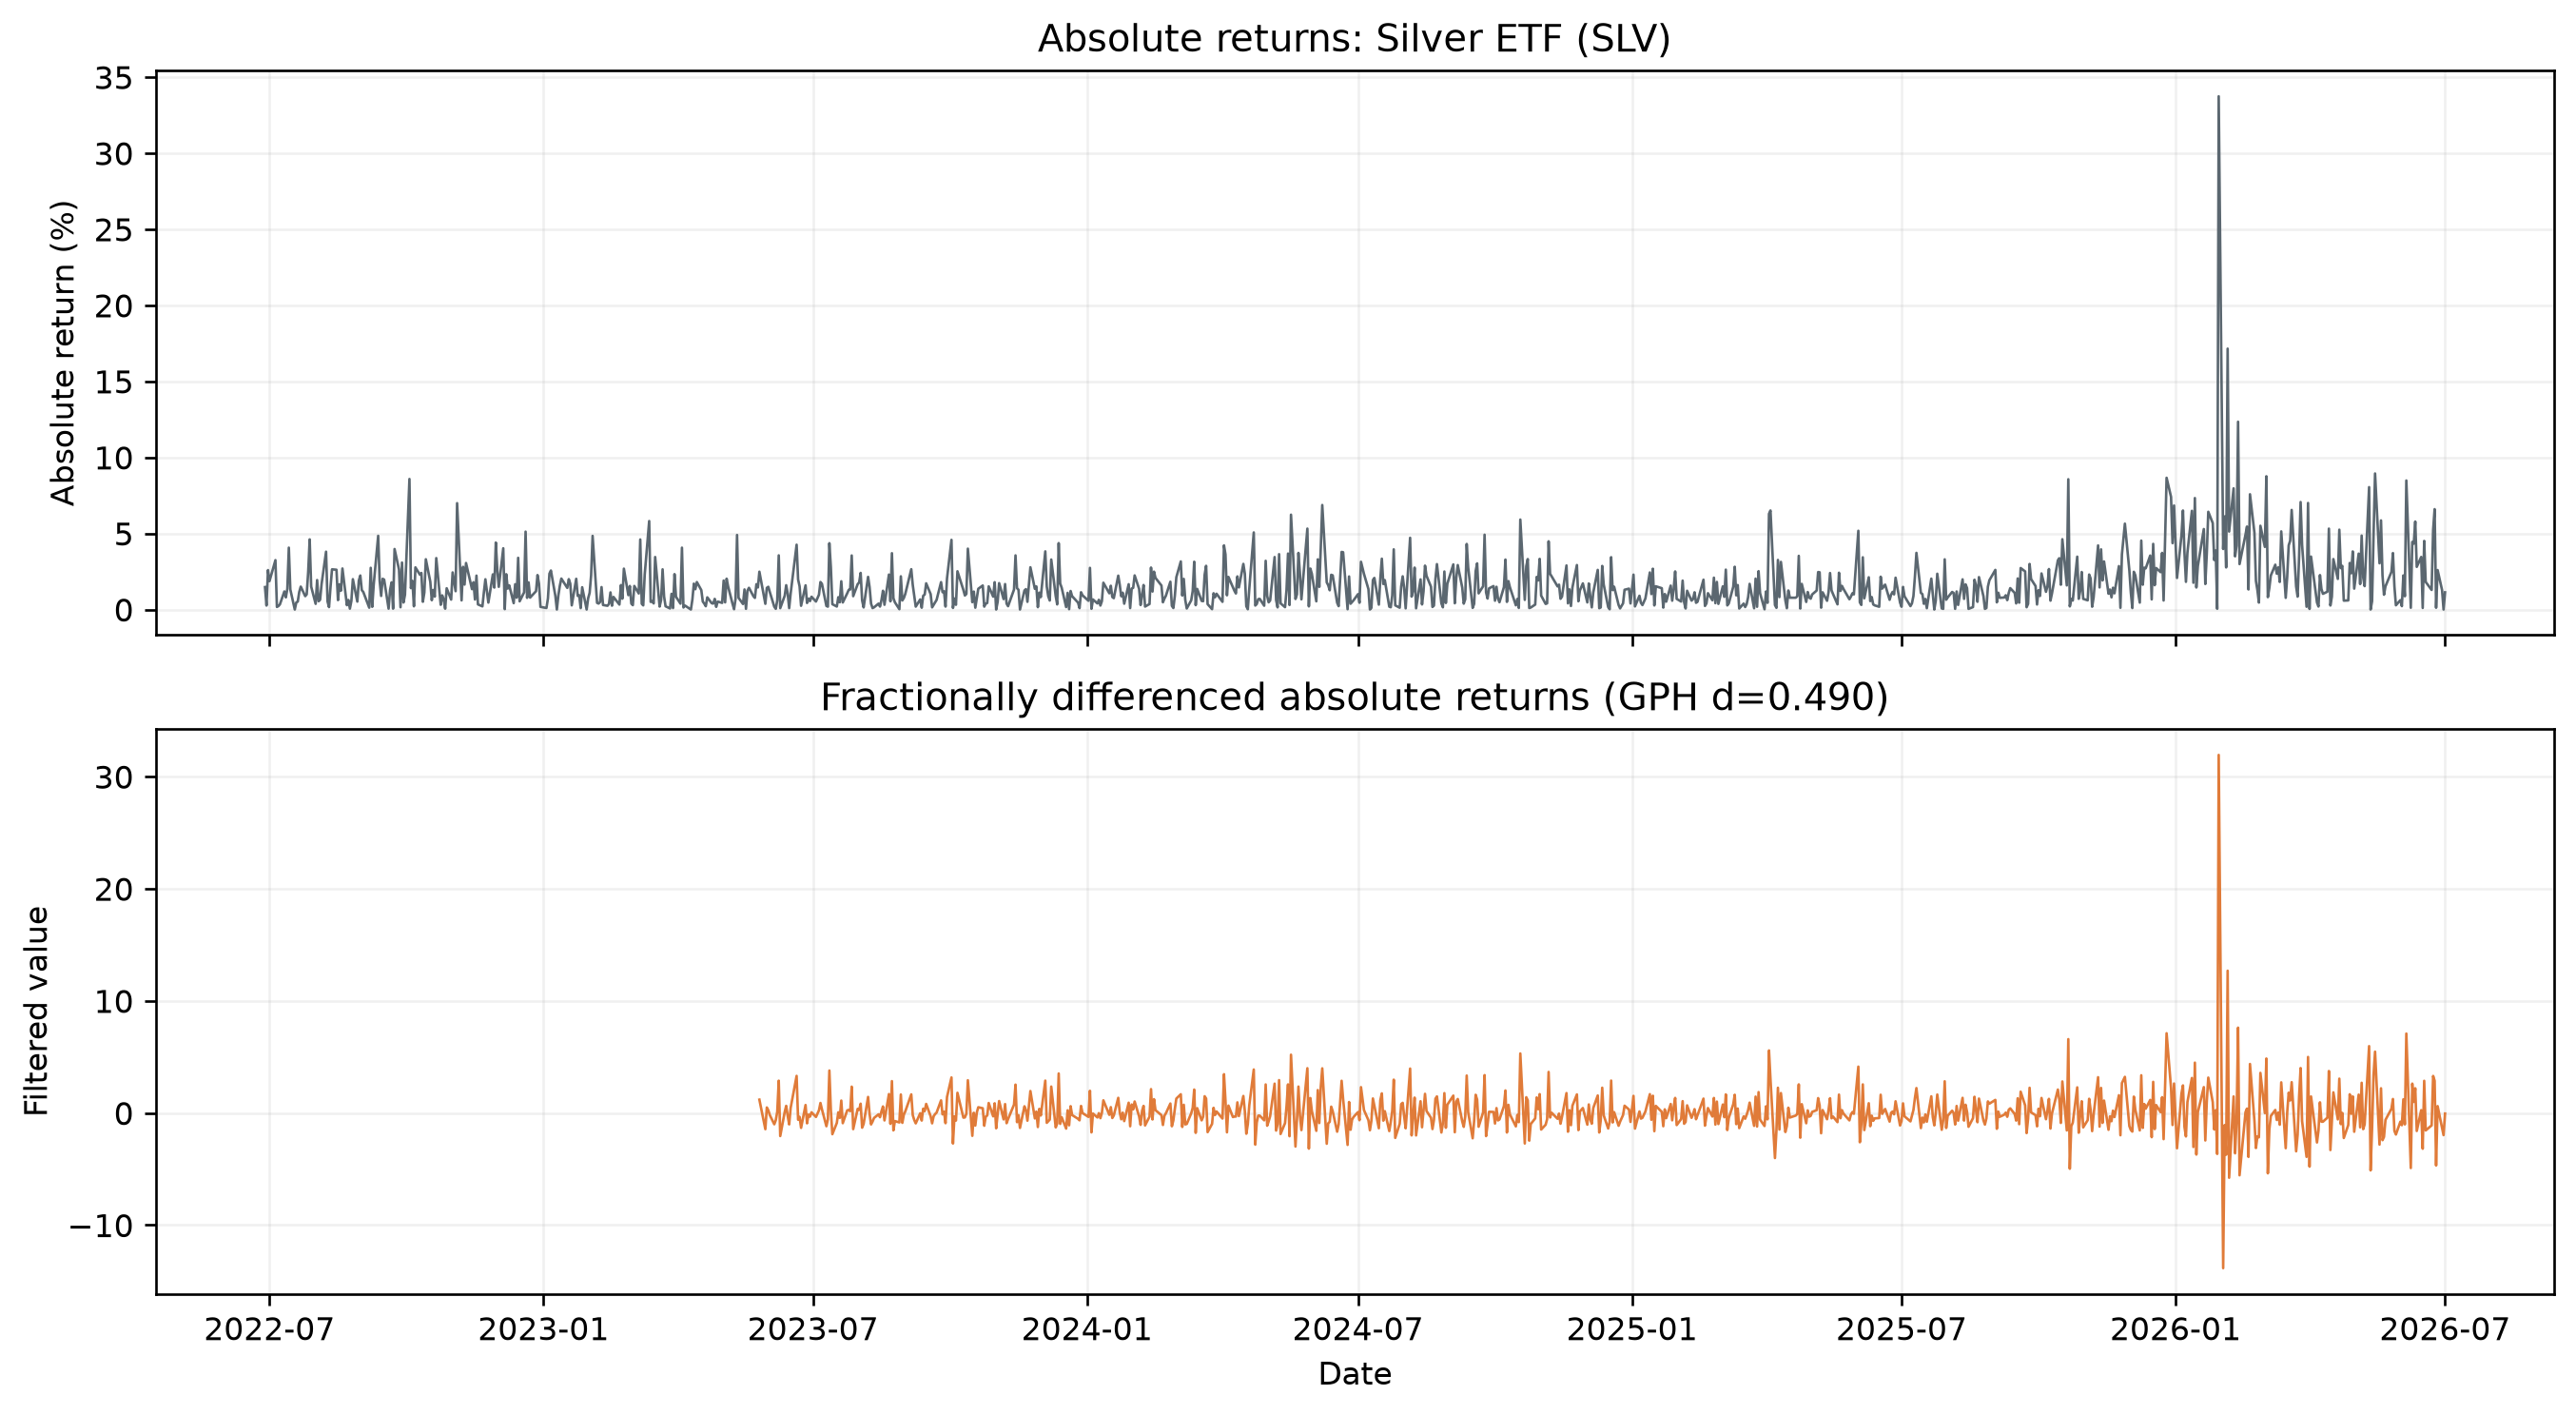
\includegraphics[width=0.86\textwidth]{img/team7_empirical/arfima_fd_silver.png}
\caption{Current LSE absolute returns and fractional filtering; the plotted GPH estimates are 0.452 for GLD and 0.490 for SLV}
\label{fig:t7-fractional-differencing}
\end{figure}

The result requires a stronger qualification than the original standalone
article supplied. In the elementary ARFIMA case, covariance stationarity
requires $d<0.5$; both frozen published point estimates exceed that boundary,
whereas the current LSE estimates lie just below it, with SLV at the imposed
search cap. The evidence is therefore compatible with very strong or
boundary-sensitive persistence, but it does not establish a stable
covariance-stationary ARFIMA law.
Bandwidth sensitivity, alternative long-memory estimators and structural-break
controls remain necessary before assigning a stable economic interpretation.

\clearpage
\section{Limitations and Downstream Resolution}

\paragraph{Limitations of this empirical layer.}
The evidence is conditional on daily frequency and ETF proxies for spot
metals. The chapter deliberately juxtaposes frozen Yahoo tables with current
LSE figures; their estimates are not pooled. Calendar synchronization, the
SPY and DXY-formula proxies, and the use of a yield change alongside asset
returns affect interpretation.
Static and rolling correlations and HC1 regressions are descriptive; they do
not identify monetary, inflationary or geopolitical shocks. Normal-innovation
GARCH does not represent leverage asymmetry, heavy-tailed innovations,
structural breaks or jump arrivals. The GPH result is boundary-sensitive. In
addition, the preserved article tables and repository outputs contain minor
version drift in some AR(1) standard errors; this chapter reports the published
article snapshot and does not disguise it as a fresh recomputation.

\paragraph{Developments already completed in the unified thesis.}
The standalone article described continuous-time stochastic volatility,
option calibration and company valuation as ``next steps.'' They are no
longer future work here. Chapter~8 develops Black--Scholes, Heston,
Bates--Poisson and Bates--Hawkes dynamics, including clustered jumps.
Chapter~9 calibrates the option-pricing layer to a dated GLD surface under the
risk-neutral measure $\mathbb Q$. Chapters~10 and~11 build the production,
cost and DCF interfaces, while Chapters~12 and~13 propagate the four gold-price
engines through a common Barrick valuation experiment and validate their
comparability. The present chapter supplies the historical empirical
motivation for those completed layers; it is not their terminal result.

\paragraph{Residual research agenda.}
Work that remains genuinely open includes a same-date, multi-provider rebuild
of the historical panel; Student-$t$, asymmetric and regime-switching
volatility benchmarks; rolling or expanding-window re-estimation; formal
causal identification of macroeconomic shocks; and robust long-memory tests
under breaks. The most important interface question is the mapping between
historical $\mathbb P$ dynamics and option-implied $\mathbb Q$ parameters.
An augmented filtration that converts textual macroeconomic and geopolitical
information into measurable state variables is also a credible machine-
learning extension, but it is outside the evidence completed in this thesis.

The decision point is therefore precise. ARIMA remains valid for integrated
levels and GARCH remains useful for discrete-time conditional variance, but
low-dimensional historical mean models cannot jointly represent the option
smile, continuous stochastic variance and discontinuous repricing required by
the valuation. Chapter~8 introduces that model layer without treating an
option-implied distribution as an automatic physical-measure forecast.

% AUTO-GENERATED by Github-Branch/tools/build_unified_source.ps1.
% Do not edit this file directly: update the transformation manifest instead.
\chapter{Affine Stochastic Models with Stochastic Volatility and Jumps}
\chapterstatus{Edited reuse from Team 6. Synthetic illustrations and calibration claims are excluded; formula parity and branch conventions remain under review.}
\sourceassetnote
\section{From Conditional Variance to a Continuous-Time Pricing Baseline}

Chapter~7 established a discrete-time empirical fact: the conditional variance
of gold returns is dynamic and persistent even when the conditional mean is
weak. This chapter changes purpose as well as time scale. Its task is not to
replace GARCH as an econometric diagnostic, but to define risk-neutral
continuous-time processes that can price an option surface and later generate
internally consistent scenario paths.

Black--Scholes--Merton is the baseline. For a European claim
$C=C(S,t)$ with constant volatility $\sigma$, the replication argument gives
\[
 C_t+\frac{1}{2}\sigma^2S^2C_{SS}+rSC_S-rC=0.
\]
After changing from calendar time to time-to-maturity, taking logarithmic
moneyness as the spatial variable and rescaling the dependent variable, this
parabolic equation reduces to the standard heat equation. The connection is a
mathematical transformation that makes diffusion tools available to finance;
it is not a claim that Black--Scholes or Heston were generically ``taken from
physics.'' The same baseline also makes the later departures precise: constant
variance is replaced by a state process, and continuous paths are augmented by
jumps.

\section{Limits of the Classical Black–Scholes Framework}
\subsection{Continuous Paths and the Absence of Jumps}

The Black-Scholes-Merton framework fundamentally assumes that the underlying asset price follows a Geometric Brownian Motion (GBM). Under the risk-neutral measure $\mathbb{Q}$, the Stochastic Differential Equation (SDE) governing the asset is:
$$dS_t = r S_t dt + \sigma S_t dW_t^\mathbb{Q}$$
where $r$ is the constant risk-free rate, $\sigma$ is the constant volatility, and $W_t^\mathbb{Q}$ is a standard Brownian motion.A defining mathematical property of standard Brownian motion is that its sample paths are almost surely continuous. Because the only source of randomness in the GBM equation is the infinitesimal increment $dW_t^\mathbb{Q}$, the asset price process $S_t$ strictly inherits this continuity.We can formalize this by defining the left limit of the price process at time $t$ as $S_{t^-} = \lim_{s \to t^-} S_s$. The continuous-path assumption rigorously implies that the price immediately before the instant $t$ and the price at the exact instant $t$ are identical. Consequently, the instantaneous price jump, denoted as $\Delta S_t$, is strictly zero:
$$\Delta S_t = S_t - S_{t^-} = 0 \quad \text{with probability 1}$$
\subsubsection{The Empirical Contradiction and Delta Hedging Failure}

While mathematically elegant, this assumption strongly contradicts the reality of financial markets. Real-world assets frequently experience abrupt price discontinuities—or "jumps"—caused by overnight market closures, macroeconomic announcements, or sudden corporate defaults. In these practical scenarios, the jump size is not zero ($\Delta S_t \neq 0$).This limitation is critical because the entire Black-Scholes pricing logic relies on Delta hedging to continuously eliminate risk. To construct a perfectly risk-free portfolio, a trader must be able to continuously rebalance the underlying asset as its price smoothly diffuses. If an asset price gaps instantaneously from $100$ to $80$, the trader physically and mathematically cannot trade at the intermediate prices (e.g., $95$, $90$).When a jump occurs, the first-order Taylor expansion (Itô's Lemma) used to hedge the option breaks down. The continuous dynamic replication fails, making the market "incomplete" and leaving the hedged portfolio exposed to severe directional risk. Therefore, to safely price and hedge in real-world conditions, the framework must be expanded beyond pure diffusions to incorporate discontinuous stochastic processes.
\subsection{Constant Volatility and the Volatility Smile}
A core structural assumption of the Black-Scholes-Merton model is that the instantaneous volatility of the underlying asset returns, denoted by $\sigma$, is a deterministic constant over the life of the derivative. Under this assumption, the theoretical price of a European Call option $C_{BS}$ is given by the closed-form solution:
$$C_{BS}(S_t, K, \tau, \sigma) = S_t N(d_1) - K e^{-r\tau} N(d_2)$$
where $\tau = T - t$ is the time to maturity, and $d_1, d_2$ are defined as:
$$d_1 = \frac{\ln(S_t / K) + (r + \frac{1}{2}\sigma^2)\tau}{\sigma \sqrt{\tau}}, \quad d_2 = d_1 - \sigma \sqrt{\tau}$$
Because the partial derivative of the option price with respect to volatility—known as Vega ($\mathcal{V}$)—is strictly positive everywhere:$$\mathcal{V} = \frac{\partial C_{BS}}{\partial \sigma} = S_t \sqrt{\tau} \phi(d_1) > 0$$the Black-Scholes pricing function is strictly monotonically increasing with respect to $\sigma$. This mathematical property guarantees that for any observed, arbitrage-free market price of an option $C_{mkt}$, there exists a unique positive root $\sigma_{imp}$ that equates the theoretical model to the market reality. This root is defined as the Implied Volatility:
$$C_{mkt}(K, \tau) = C_{BS}(S_t, K, \tau, \sigma_{imp})$$
If the foundational assumption $d\sigma = 0$ were empirically correct, solving this inverse problem across a spectrum of different strike prices $K$ should yield a constant value for $\sigma_{imp}$. Geometrically, plotting $\sigma_{imp}$ as a function of $K$ would result in a perfectly flat horizontal line.However, empirical market data systematically violates this condition. By extracting implied volatilities across various strikes for a given maturity, one observes that:
$$\frac{\partial \sigma_{imp}}{\partial K} \neq 0 \quad \text{and} \quad \frac{\partial^2 \sigma_{imp}}{\partial K^2} > 0$$
This non-linear relationship forms a convex curve commonly referred to as the volatility smile or, more typically in equity markets, a pronounced downward-sloping volatility skew. Deep out-of-the-money (OTM) put options command significantly higher implied volatilities than at-the-money (ATM) options. This structural deformation occurs because market participants inherently price in the "fat tails" (excess kurtosis) and negative skewness of the real-world return distributions. To reconcile the mathematical model with observed market dynamics, the classical framework must be abandoned in favor of models where volatility itself follows a stochastic diffusion process.

% Asset/code block omitted pending provenance acceptance.
\subsection{Motivation for Jump and Stochastic Volatility Models}
Given the empirical failures of continuous sample paths and constant volatility assumptions, the classical Black-Scholes-Merton framework must be expanded. To accurately capture both the short-term and long-term topological features of the implied volatility surface, modern quantitative finance introduces two distinct but complementary mathematical extensions: Stochastic Volatility (SV) and Jump-Diffusion (JD) processes.
\subsubsection{The Case for Stochastic Volatility (Long-Maturity Skew)}
To capture the empirical observation that volatility fluctuates and clusters over time, SV models relax the assumption that $d\sigma = 0$. Instead, the variance $v_t = \sigma_t^2$ is promoted to a strictly positive state variable governed by its own stochastic differential equation, typically a mean-reverting square-root diffusion such as the Cox-Ingersoll-Ross (CIR) process. The coupled system under the risk-neutral measure takes the form:
$$dS_t = r S_t dt + \sqrt{v_t} S_t dW_t^S$$
$$dv_t = \kappa(\theta - v_t)dt + \xi \sqrt{v_t} dW_t^v$$

where the Brownian motions $dW_t^S$ and $dW_t^v$ are correlated ($d\langle W^S, W^v \rangle_t = \rho dt$). The correlation parameter $\rho < 0$ mathematically generates the "leverage effect," naturally producing a downward-sloping volatility skew. However, because SV diffusions are continuous, the variance requires time to accumulate. As time to maturity approaches zero ($\tau \to 0$), the diffusion variance $\int_t^T v_s ds$ converges to zero, causing the theoretical short-term volatility skew to flatten out, which contradicts the steep short-term smiles observed in equity markets.
\subsubsection{The Case for Jump Processes (Short-Maturity Skew)}
To address short-maturity pricing effects and the possibility of sudden market
repricing, jump--diffusion models augment the continuous Brownian component with
a jump component driven by a Poisson process $N_t$. The asset dynamics are
modified as
\[
    \frac{dS_t}{S_{t^-}}
    =
    (r-\lambda k)\,dt+\sigma\,dW_t+(e^J-1)\,dN_t,
    \qquad
    k:=\mathbb{E}^{\mathbb{Q}}[e^J-1],
\]
where $\lambda$ is the jump intensity and $J$ is the logarithmic jump size. The
compensator $\lambda k$ ensures that the discounted price is a martingale under
the pricing measure. Jumps can generate heavy tails and skewness even over short
time horizons, because a discontinuous move may occur before the diffusion
component has accumulated substantial variance. Over longer horizons, however,
the standardized contribution of finite-variance independent jumps becomes less
pronounced: the total variance grows linearly with maturity, while skewness and
excess kurtosis scale down. As a result, pure jump--diffusion models typically
struggle to reproduce persistent long-maturity volatility skews.


\textbf{Synthesis}
Ultimately, neither framework is independently sufficient. Jump processes are mathematically essential to capture abrupt discontinuities and price short-maturity out-of-the-money options, while stochastic volatility is required to model the persistent, mean-reverting nature of market variance and price long-maturity options. This duality motivates the transition toward unified affine jump-diffusion frameworks, such as the Bates model, which integrate both mechanisms to consistently describe the entire volatility surface.

% ---- next approved source slice ----

\section{Poisson Processes and Jump Times}
\subsection{Counting Processes}
To overcome the strict continuity assumptions of the classical diffusion framework, we must introduce mathematical structures capable of modeling discrete, isolated events occurring randomly in continuous time. The foundational building block for such models is the counting process.
Let $(\Omega, \mathcal{F}, \mathbb{P})$ be a probability space equipped with a filtration $\{\mathcal{F}_t\}_{t \ge 0}$ satisfying the usual conditions. A stochastic process $\{N_t\}_{t \ge 0}$ is defined as a counting process if it represents the total number of specific events that have occurred up to and including time $t$.
Mathematically, $\{N_t\}_{t \ge 0}$ must satisfy the following fundamental properties:
\begin{enumerate}
    \item $N_0 = 0$ almost surely
    \item For any time $t \ge 0$, $N_t$ takes values in the set of non-negative integers $\mathbb{N}_0 = \{0, 1, 2, \dots\}$
    \item The paths of the process are non-decreasing: for any two time points $s < t$, we have $N_s \le N_t$ almost surely.
    \item For any $s < t$, the increment $(N_t - N_s)$ represents the strictly non-negative integer number of events occurring in the time interval $(s, t]$.
\end{enumerate}
A crucial topological feature of a counting process is its sample path trajectory. Unlike standard Brownian motion $W_t$, which possesses continuous sample paths, the counting process $N_t$ is a piecewise constant step function. Its paths belong to the space of càdlàg functions (right-continuous with left limits).
If we denote the random arrival time of the $n$-th event as $\tau_n$, where $0 < \tau_1 < \tau_2 < \dots < \tau_n < \dots$, the instantaneous behavior of the process at an arrival time exhibits a discrete jump:
$$\Delta N_{\tau_n} = N_{\tau_n} - N_{\tau_n^-} = 1$$
where $N_{\tau_n^-} = \lim_{s \to \tau_n^-} N_s$. 

At all other times $t \neq \tau_n$, the differential $dN_t$ is strictly zero.Consequently, the counting process provides the exact mathematical language required to formalize the arrival of abrupt price discontinuities in financial markets, completely independent of the continuous diffusion component.

% Asset/code block omitted pending provenance acceptance.
\subsection{Homogeneous Poisson Processes}
While a general counting process provides the structural framework for discrete jumps, we must specify the probabilistic laws governing their arrival. The most fundamental model for random, independent jump arrivals in continuous time is the Homogeneous Poisson Process.
Given the filtered probability space $(\Omega, \mathcal{F}, \mathbb{P})$, a counting process $\{N_t\}_{t \ge 0}$ is defined as a Homogeneous Poisson Process with constant intensity (or rate) parameter $\lambda > 0$ if it satisfies the following axiomatic properties:
\begin{enumerate}
    \item \textbf{Independent Increments:} For any sequence of time points $0 \le t_0 < t_1 < \dots < t_n$, the random variables representing the number of events in each interval, $(N_{t_1} - N_{t_0}), (N_{t_2} - N_{t_1}), \dots, (N_{t_n} - N_{t_{n-1}})$, are mutually independent. This implies that the probability of a future jump is strictly independent of the past filtration $\mathcal{F}_s$ for $s < t$.
    \item \textbf{Stationary Increments:} The distribution of the number of events in any time interval depends exclusively on the length of the interval, and not on its absolute position in time.
    \item \textbf{Infinitesimal Transition Probabilities:} In an infinitesimally small time interval $dt$, the probability of observing exactly one jump is proportional to $\lambda$, while the probability of observing multiple simultaneous jumps is negligible. Formally:
    $$\mathbb{P}[N_{t+dt} - N_t = 1] = \lambda dt + o(dt)$$
    $$\mathbb{P}[N_{t+dt} - N_t \ge 2] = o(dt)$$
    $$\mathbb{P}[N_{t+dt} - N_t = 0] = 1 - \lambda dt + o(dt)$$
\end{enumerate}

A direct mathematical consequence of these axioms is that for any finite time interval of length $\tau = t - s > 0$, the increment $(N_t - N_s)$ follows a Poisson distribution with parameter $\lambda \tau$. The probability mass function (PMF) of observing exactly $k$ jumps in this interval is given by:
$$\mathbb{P}[N_t - N_s = k] = \frac{e^{-\lambda \tau} (\lambda \tau)^k}{k!}, \quad \text{for } k = 0, 1, 2, \dots$$
This specific distribution perfectly defines the moments of the process. For a Homogeneous Poisson Process, both the expected value and the variance grow linearly with time, scaled by the intensity $\lambda$:
$$\mathbb{E}[N_t] = Var(N_t) = \lambda t$$
In the context of quantitative finance, $\lambda$ represents the mean arrival rate of market shocks per unit of time (e.g., jumps per year). By assigning this strict probabilistic structure, we can mathematically price the probability of observing $k$ extreme market events before an option's maturity date.
\subsection{Waiting Times and Exponential Interarrival Structure}
The Homogeneous Poisson Process can be equivalently defined through the continuous time intervals elapsed between consecutive jumps. Rather than counting the number of events in a fixed time window, we analyze the random time required for the next event to occur.Let $\tau_1, \tau_2, \dots, \tau_n$ be the strictly increasing random arrival times of the jumps, where $\tau_1$ is the time of the first event. We define the sequence of interarrival times (or waiting times) $\{T_n\}_{n \ge 1}$ as:
$$T_1 = \tau_1$$
$$T_n = \tau_n - \tau_{n-1}, \quad \text{for } n \ge 2$$
For a Homogeneous Poisson Process with intensity $\lambda > 0$, the interarrival times $T_1, T_2, \dots$ form a sequence of independent and identically distributed (i.i.d.) random variables following an Exponential distribution.The probability density function (PDF) of each interarrival time $T_n$ is:
$$f_T(t) = \lambda e^{-\lambda t}, \quad \text{for } t \ge 0$$
Integrating this density, we can determine the probability that the waiting time exceeds a certain threshold $t$. In reliability engineering and mathematical finance, this is known as the survival probability, formalized as $\mathbb{P}[X > x] = 1 - F_X(x)$. For our interarrival times, the survival probability assumes the explicit form:
$$\mathbb{P}[T_n > t] = \int_t^\infty \lambda e^{-\lambda s} ds = e^{-\lambda t}$$
The expected waiting time between two consecutive jumps is the reciprocal of the intensity parameter:
$$\mathbb{E}[T_n] = \frac{1}{\lambda}$$
This provides a highly intuitive financial metric: if a specific market shock is modeled with an intensity of $\lambda = 0.5$ events per year, the expected waiting time between such shocks is $2$ years.
\paragraph{The Memoryless Property}~\\
A profound structural consequence of the exponential interarrival times is the memoryless property. Mathematically, for any $s, t \ge 0$:
$$\mathbb{P}[T_n > s + t \mid T_n > s] = \mathbb{P}[T_n > t]$$
In the context of financial markets, this property implies that the homogeneous jump process possesses no memory of the past. If a market has survived for a time $s$ without experiencing a crash, the conditional probability of surviving for an additional time $t$ depends solely on $t$ and $\lambda$. The risk of a jump arrival does not deterministically "age" or accumulate over time; the probability of an instantaneous shock remains perpetually constant.
\subsection{Financial Interpretation of Random Jump Arrivals}
The rigorous mathematical framework of the Poisson process provides a natural language for describing the mechanics of information flow in financial markets. In classical diffusion models, asset prices evolve continuously, which implicitly assumes that new information arrives in a smooth, continuous stream. While this adequately models normal daily trading noise and minor order-book imbalances, it fails to capture the true nature of critical macroeconomic and firm-specific news.

In reality, highly impactful information arrives discretely. The random jump times $\tau_1, \tau_2, \dots$ generated by the Poisson process map directly to the exact moments these sudden information shocks hit the market. We can broadly categorize these random arrivals into two distinct financial classes:
\begin{enumerate}
    \item \textbf{Idiosyncratic (Firm-Specific) Shocks:} These are localized events affecting a single asset, such as an unexpected earnings announcement, a sudden CEO resignation, a merger and acquisition (M\&A) bid, or a corporate default.
    \item \textbf{Systemic (Macroeconomic) Shocks:} These represent broader market disruptions affecting entire sectors or indices, such as surprise interest rate changes by central banks, geopolitical conflicts, or sudden liquidity crises.
\end{enumerate}
The intensity parameter $\lambda$ serves as a quantitative measure of the market's "hazard rate." A low $\lambda$ characterizes a stable economic environment with rare discontinuities, whereas a high $\lambda$ reflects a volatile, distressed market regime where sudden shocks are expected to arrive with higher frequency.
\paragraph{The Bridge to Compound Processes}~\\
While the simple counting process $N_t$ successfully models when a market shock occurs (yielding a jump of magnitude $\Delta N_t = 1$), it does not quantify the economic severity of the shock. An interest rate hike might cause a $2\%$ drop in an equity index, whereas a corporate bankruptcy could erase $80\%$ of a stock's value instantaneously.

To build a complete asset pricing model, the fixed unit jump of the counting process must be replaced with a random variable representing the jump size. This mathematical evolution—combining the random arrival times of the Poisson process with random price impacts—leads directly to the formulation of the Compound Poisson Process and Jump-Diffusion models.
\section{Compound Poisson Processes and Jump--Diffusions}
\subsection{Random Jump Sizes}

The Poisson process introduced previously provides a natural description of the random arrival times of events. In order to construct processes with jumps, it is necessary to associate to each jump time a random amplitude.

Let $(\Omega, \mathcal{F}, \mathbb{P})$ be a probability space and let $\{N_t\}_{t \geq 0}$ be a Poisson process with intensity $\lambda > 0$. We consider a sequence of random variables $\{Y_i\}_{i \geq 1}$ defined on the same probability space, such that:

\begin{itemize}[label = --]
    \item the random variables $Y_i$ are independent and identically distributed;
    \item the sequence $\{Y_i\}$ is independent of the process $\{N_t\}_{t \geq 0}$.
\end{itemize}

The random variables $Y_i$ represent the jump sizes and take values in $\mathbb{R}$. This construction allows one to associate to each jump time $\tau_i$ of the Poisson process a mark $Y_i$, thus obtaining a marked point process.

From a modelling perspective, the independence assumption reflects the fact that the arrival times of jumps and their magnitudes are driven by distinct sources of randomness.

\medskip

This framework naturally leads to the construction of jump processes by summing the contributions of individual jumps.
\subsection{Compound Poisson Sums}

\begin{definition}
The stochastic process $\{X_t\}_{t \geq 0}$ defined by
\[
X_t = \sum_{i=1}^{N_t} Y_i
\]
is called a \emph{compound Poisson process}.
\end{definition}

By convention, the sum is taken to be zero when $N_t = 0$.

Conditionally on the event $\{N_t = n\}$, the random variable $X_t$ is equal to the sum of $n$ independent random variables with the same distribution as $Y_1$. Therefore, its distribution is given by the $n$-fold convolution of the law of $Y_1$.

Using the law of total expectation, one obtains:
\[
\mathbb{E}[X_t] = \mathbb{E}[N_t] \mathbb{E}[Y_1] = \lambda t \, \mathbb{E}[Y_1],
\]
and
\[
\mathrm{Var}(X_t) = \lambda t \, \mathbb{E}[Y_1^2].
\]

The process $\{X_t\}_{t \geq 0}$ has independent and stationary increments and is therefore a L\'evy process. Its sample paths are piecewise constant, right-continuous with left limits (c\`adl\`ag), with jumps occurring at the jump times of the Poisson process.

\medskip

An equivalent representation is obtained by introducing the discrete-time random walk
\[
R(n) = \sum_{i=1}^{n} Y_i, \quad n \in \mathbb{N},
\]
so that
\[
X_t = R(N_t).
\]

This representation emphasizes that a compound Poisson process can be viewed as a random walk observed at random times.

\medskip

A fundamental property of compound Poisson processes is that they belong to the class of L\'evy processes with \emph{finite activity}, meaning that the number of jumps on any finite time interval is almost surely finite.

More precisely, for any $t \geq 0$, the number of jumps of $X_t$ on $[0,t]$ is equal to $N_t$, which is finite with probability one.

\medskip

Finally, the characteristic function of $X_t$ is given by
\[
\mathbb{E}\left[e^{iu X_t}\right] = \exp\left( \lambda t \left( \mathbb{E}[e^{iuY_1}] - 1 \right) \right),
\]
which follows from conditioning on $N_t$ and using the independence of the jump sizes.
This expression highlights the infinite divisibility of the distribution of $X_t$ and plays a central role in the analysis of jump processes.
\subsection{From Diffusions to Jump--Diffusions}


The compound Poisson process captures the abrupt component of price
dynamics, but its sample paths are piecewise constant between jumps
and therefore cannot accommodate the continuous fluctuations that
Brownian motion describes so effectively. A realistic model of the
underlying asset price must superpose the two mechanisms: a diffusive
component for the ordinary trading noise and a compound Poisson
component for the discontinuous revaluations of the underlying
asset. This programme, originally proposed by
Merton, yields the class of \emph{jump--diffusion} models.

Let $(\Omega, \mathcal{F}, \{\mathcal{F}_t\}_{t\geq 0}, \mathbb{P})$
be a filtered probability space supporting
a standard Brownian motion $\{W_t\}_{t\geq 0}$, a Poisson process
$\{N_t\}_{t\geq 0}$ with intensity $\lambda > 0$ and a sequence
$\{Y_i\}_{i\geq 1}$ of i.i.d.\ real random variables with
$\mathbb{E}[e^{Y_1}] < \infty$. We assume that $W$, $N$ and
$\{Y_i\}_{i\geq 1}$ are mutually independent and that
$\{\mathcal{F}_t\}_{t\geq 0}$ is the filtration jointly generated by
them, so that $W$ and $N$ are Brownian and Poisson relative to this
filtration.
The asset price $\{S_t\}_{t\geq 0}$ is then postulated to evolve
according to the stochastic differential equation
\begin{equation}
    dS_t = \mu\, S_{t^-}\, dt + \sigma\, S_{t^-}\, dW_t
         + S_{t^-}\!\left(e^{Y} - 1\right) dN_t,
    \qquad S_0 > 0,
\end{equation}
with constants $\mu \in \mathbb{R}$, $\sigma > 0$ and $Y$ denoting the
generic element of the sequence $\{Y_i\}_{i\geq 1}$ that provides the
jump sizes at the successive arrival times of $N$. The left limit
$S_{t^-}$ appears in the Brownian and Poisson integrals as required
by the predictability of the integrand: between jumps
$S_{t^-} = S_t$, so the first two terms reproduce the usual geometric
Brownian dynamics, whereas at a jump time $\tau_i$ of $N$ the
increment of the third term contributes $S_{\tau_i^-}(e^{Y_i} - 1)$,
so that
\[
    S_{\tau_i} = S_{\tau_i^-}\, e^{Y_i}.
\]
The sample paths of $\{S_t\}_{t\geq 0}$ are therefore almost surely
c\`adl\`ag, strictly positive, and coincide with a geometric Brownian
motion on each stochastic interval between two consecutive arrival
times of $N$; at each arrival time they are multiplied by the
independent random factor $e^{Y_i}$.

An explicit solution of~\sourceref{eq:jumpdiff_SDE} can be obtained by
factoring $S_t$ into its continuous and pure-jump components and
applying the It\^o--Doeblin formula for jump processes. Define
\[
    X_t = S_0 \exp\!\left\{\sigma W_t
        + \left(\mu - \tfrac{1}{2}\sigma^2\right) t\right\},
    \qquad
    J_t = \prod_{i=1}^{N_t} e^{Y_i},
\]
with the empty product equal to $1$. The process $\{X_t\}_{t\geq 0}$
is continuous and satisfies, by the It\^o formula for continuous
semimartingales,
\[
    dX_t = \mu\, X_t\, dt + \sigma\, X_t\, dW_t,
\]
while $\{J_t\}_{t\geq 0}$ is a pure-jump process whose jump at the
arrival time $\tau_i$ of $N$ equals $J_{\tau_i^-}(e^{Y_i} - 1)$, so
that in differential form
\[
    dJ_t = J_{t^-}\!\left(e^{Y} - 1\right) dN_t.
\]
Because $X$ is continuous and $J$ is a pure-jump process, their
quadratic covariation vanishes. Applying the product rule for jump
processes to $S_t = X_t J_t$ yields
\[
    dS_t = X_{t^-}\, dJ_t + J_t\, dX_t
         = \mu\, S_{t^-}\, dt + \sigma\, S_{t^-}\, dW_t
         + S_{t^-}\!\left(e^{Y} - 1\right) dN_t,
\]
which is precisely~\sourceref{eq:jumpdiff_SDE}. We have therefore
established the closed-form representation
\begin{equation}
    S_t = S_0 \exp\!\left\{\sigma W_t
        + \left(\mu - \tfrac{1}{2}\sigma^2\right) t\right\}
        \prod_{i=1}^{N_t} e^{Y_i}
        = S_0 \exp\!\left\{\sigma W_t
            + \left(\mu - \tfrac{1}{2}\sigma^2\right) t
            + \sum_{i=1}^{N_t} Y_i\right\}.
\end{equation}
The logarithmic price $\ln(S_t/S_0)$ is thus the sum of a Brownian
component with drift $\mu - \tfrac{1}{2}\sigma^2$ and an independent
compound Poisson component $\sum_{i=1}^{N_t} Y_i$ with intensity
$\lambda$ and jump-size distribution that of $Y_1$. In differential
form,
\begin{equation}
    d\ln S_t = \left(\mu - \tfrac{1}{2}\sigma^2\right) dt
             + \sigma\, dW_t + Y\, dN_t,
\end{equation}
where $Y\,dN_t$ denotes the increment of the compound Poisson process
$\sum_{i=1}^{N_t} Y_i$ at a jump time of $N$.

% Asset/code block omitted pending provenance acceptance.


Representation~\sourceref{eq:jumpdiff_sol} makes transparent the two
structural features that distinguish jump--diffusions from the
Black--Scholes dynamics. First, the
distribution of $\ln(S_t/S_0)$ is no longer Gaussian but a mixture of
Gaussians indexed by $N_t$: conditional on $\{N_t = k\}$, the log
return is normal with mean
$\bigl(\mu - \tfrac{1}{2}\sigma^2\bigr) t + \sum_{i=1}^{k} Y_i$
and variance $\sigma^2 t$, and the unconditional law aggregates these
components weighted by the Poisson probabilities
$e^{-\lambda t}(\lambda t)^k / k!$. This mixture structure generates
the excess kurtosis and asymmetric skewness that the pure-diffusion
model failed to reproduce. Secondly, with probability
$1 - e^{-\lambda t} > 0$ the trajectory $s \mapsto S_s$ exhibits at
least one discontinuity on the interval $[0,t]$, in sharp contrast
with the almost-sure continuity of the Black--Scholes price process
on the same interval. The dynamics~\sourceref{eq:jumpdiff_SDE} thus
removes the two most consequential structural limitations of the
diffusive framework simultaneously, at the cost of introducing a
second, discontinuous source of randomness whose implications for
hedging and for the uniqueness of the equivalent martingale measure
will be analysed in the next subsection.
\subsection{Drift Compensation and Risk-Neutral Dynamics}

In an arbitrage-free setting, pricing is performed under a risk-neutral probability measure $\mathbb{Q}$, equivalent to the physical measure $\mathbb{P}$, under which discounted asset prices are martingales.

More precisely, if $\{S_t\}_{t \geq 0}$ denotes the asset price process, the no-arbitrage condition requires that the discounted process satisfies
\[
e^{-rt} S_t \quad \text{is a martingale under } \mathbb{Q}.
\]

Equivalently, for all $t \geq 0$,
\[
\mathbb{E}^{\mathbb{Q}}[S_t \mid \mathcal{F}_0] = S_0 e^{rt}.
\]

In the presence of jumps, this martingale condition imposes a constraint on the drift of the process. To make this explicit, we rewrite the jump--diffusion dynamics in differential form:
\[
\frac{dS_t}{S_{t^-}} = \mu \, dt + \sigma \, dW_t + (e^{Y} - 1) dN_t.
\]

Taking expectations under $\mathbb{Q}$ and using the independence between the Brownian and Poisson components, together with the fact that $\mathbb{E}[dW_t] = 0$ and $\mathbb{E}[dN_t] = \lambda dt$, we obtain
\[
\mathbb{E}^{\mathbb{Q}}\left[\frac{dS_t}{S_{t^-}}\right] = \mu \, dt + \lambda \, \mathbb{E}[e^{Y} - 1] \, dt.
\]

The martingale condition for the discounted price process requires that the expected return equals the risk-free rate, that is
\[
\mathbb{E}^{\mathbb{Q}}\left[\frac{dS_t}{S_{t^-}}\right] = r \, dt.
\]

Comparing the two expressions yields the drift restriction
\[
\mu = r - \lambda \mathbb{E}[e^{Y} - 1].
\]

This adjustment term compensates for the average contribution of jumps, ensuring that the discounted price process remains a martingale under $\mathbb{Q}$.

It is often convenient to express the jump contribution in compensated form.
When jump sizes are random, the compensation must be applied to the marked jump
measure rather than only to the scalar Poisson process. Equivalently, setting
\[
    k:=\mathbb{E}^{\mathbb{Q}}[e^J-1],
\]
the risk-neutral dynamics can be written as
\[
    \frac{dS_t}{S_{t^-}}
    =
    r\,dt+\sigma\,dW_t^{\mathbb{Q}}
    +
    \Big((e^J-1)\,dN_t-\lambda k\,dt\Big).
\]
The bracketed term is the compensated jump contribution and has zero conditional
expectation under $\mathbb{Q}$. In the language of marked point processes, this
can be written more compactly as
\[
    \frac{dS_t}{S_{t^-}}
    =
    r\,dt+\sigma\,dW_t^{\mathbb{Q}}
    +
    \int_{\mathbb{R}}(e^y-1)\,\widetilde{N}(dt,dy),
\]
where $\widetilde{N}(dt,dy)$ denotes the compensated Poisson random measure with
mark distribution equal to the law of the jump size $J$.


\medskip

From a financial perspective, this result highlights a key difference with respect to the classical Black--Scholes framework. While in pure diffusion models the martingale condition uniquely determines the drift, in the presence of jumps the market becomes incomplete, and the equivalent martingale measure is, in general, not unique.

% ---- next approved source slice ----

\section{L\'evy Processes and Discontinuous Dynamics}

The compound Poisson processes introduced in the previous section already provide a first example of stochastic dynamics with discontinuous sample paths. Their jump activity is, however, finite on every compact time interval. In many applications, especially in quantitative finance, one needs a broader class of processes capable of combining a continuous martingale component, a drift term, and a possibly much richer jump structure. This leads naturally to the class of L\'evy processes.

L\'evy processes play a central role in modern stochastic modelling because they preserve, in continuous time, the two structural properties that make random walks tractable: independence and stationarity of increments. They therefore constitute the canonical continuous-time extension of sums of i.i.d.\ random variables and provide the natural probabilistic framework for discontinuous asset returns.
\subsection{Definition and Main Properties}

We work on a filtered probability space
\[
(\Omega,\mathcal{F},\{\mathcal{F}_t\}_{t\geq 0},\mathbb{P}),
\]
and consider a stochastic process $\{X_t\}_{t\geq 0}$ with values in~$\mathbb{R}$.

\begin{definition}
A stochastic process $\{X_t\}_{t\geq 0}$ is called a \emph{L\'evy process} if the following properties hold:
\begin{itemize}[label = --]
    \item $X_0 = 0$ almost surely;
    \item $\{X_t\}_{t\geq 0}$ has \emph{independent increments}, namely for every choice of times
    \[
    0 \leq t_0 < t_1 < \dots < t_n,
    \]
    the random variables
    \[
    X_{t_1}-X_{t_0},\; X_{t_2}-X_{t_1},\; \dots,\; X_{t_n}-X_{t_{n-1}}
    \]
    are independent;
    \item $\{X_t\}_{t\geq 0}$ has \emph{stationary increments}, namely for every $s,t \geq 0$ the law of
    \[
    X_{t+s}-X_s
    \]
    depends only on $t$;
    \item $\{X_t\}_{t\geq 0}$ is \emph{stochastically continuous}, that is, for every $\varepsilon > 0$ and every $t \geq 0$,
    \[
    \lim_{h\to 0}\mathbb{P}\bigl(|X_{t+h}-X_t|>\varepsilon\bigr)=0;
    \]
    \item the sample paths are almost surely c\`adl\`ag.
\end{itemize}
\end{definition}

\begin{remark}
The c\`adl\`ag regularity of the sample paths can in fact be derived from the remaining four properties: any process satisfying the first four conditions of the definition admits a modification whose trajectories are almost surely c\`adl\`ag (see Sato, 1999, Theorem~11.5). We include it in the definition in order to fix the version of the process with which we work throughout.
\end{remark}

The definition isolates the continuous-time analogue of a random walk. Indeed, if one observes a L\'evy process only on a deterministic grid $0,\Delta,2\Delta,\dots$, then the increments
\[
X_{\Delta}-X_0,\quad X_{2\Delta}-X_{\Delta},\quad \dots,\quad X_{n\Delta}-X_{(n-1)\Delta}
\]
are independent and identically distributed by stationarity and independence of increments. Thus the discretely sampled process
\begin{equation}
S_n^{(\Delta)} := X_{n\Delta}
\end{equation}
is a random walk.

Conversely, a L\'evy process may be viewed as a continuous-time interpolation principle for random walks. This interpretation is fundamental, because it explains why L\'evy processes inherit many structural properties that are familiar from discrete-time probabilistic models.

\medskip

A first immediate consequence of the definition is the following.

\begin{theorem}[Increment identity]
Let $\{X_t\}_{t\geq 0}$ be a L\'evy process. Then for every $0\leq s<t$,
\begin{equation}
X_t-X_s \overset{d}{=} X_{t-s}.
\end{equation}
\end{theorem}

\begin{proof}
By stationarity of increments, the law of $X_t-X_s$ depends only on the time difference $t-s$. Evaluating this increment over the interval $[0,t-s]$ yields
\[
X_t-X_s \overset{d}{=} X_{t-s}-X_0.
\]
Since $X_0=0$ almost surely, the claim follows.
\end{proof}

This identity shows that the one-dimensional marginal laws of a L\'evy process are completely determined by the family of increment distributions.

\medskip

Another important property concerns infinite divisibility. Since for any integer $n\geq 1$ one may decompose the interval $[0,t]$ into $n$ subintervals of equal length, one has
\[
X_t
=
\sum_{k=1}^{n}\bigl(X_{kt/n}-X_{(k-1)t/n}\bigr),
\]
where the summands are independent and identically distributed, each with the same law as $X_{t/n}$. Hence the law of $X_t$ is infinitely divisible.

\begin{theorem}[Infinite divisibility of marginal laws]
For every $t\geq 0$, the distribution of $X_t$ is infinitely divisible.
\end{theorem}

\begin{proof}
Fix $t>0$ and $n\in\mathbb{N}$. Write
\[
X_t
=
\sum_{k=1}^{n}\bigl(X_{kt/n}-X_{(k-1)t/n}\bigr).
\]
By independence of increments, the $n$ summands are independent. By stationarity of increments, they are identically distributed. Therefore the law of $X_t$ is the $n$-fold convolution of the law of $X_{t/n}$, and since $n$ is arbitrary, the distribution is infinitely divisible.
\end{proof}

This fact is not secondary. It is one of the key structural fingerprints of the class: every L\'evy process generates an infinitely divisible family of marginal laws. The converse also holds: infinitely divisible distributions are precisely the distributions that arise at fixed times from L\'evy processes, and this constitutes one of the deep consequences of the L\'evy--Khintchine representation theorem developed below.

\begin{remark}
Every L\'evy process is a strong Markov process. This follows from the independence of increments: for any stopping time~$\tau$, the future evolution $\{X_{\tau+t}-X_\tau\}_{t\geq 0}$ is independent of $\mathcal{F}_\tau$ and has the same law as $\{X_t\}_{t\geq 0}$. The Markov property is of central importance in financial applications, as it underlies the partial integro-differential equations used for option pricing under L\'evy dynamics.
\end{remark}
\subsection{Brownian Motion and Compound Poisson as Special Cases}

The definition above contains, as special cases, both the continuous diffusive model and the finite-activity jump model developed previously. This is one of the main reasons why the L\'evy framework is so useful: it unifies in a single class several stochastic mechanisms that, at first sight, may appear rather different.
\subsubsection{Brownian Motion}

Let $\{W_t\}_{t\geq 0}$ be a standard Brownian motion. Then:
\begin{itemize}[label = --]
    \item $W_0=0$ almost surely;
    \item Brownian motion has independent increments;
    \item for every $s,t\geq 0$,
    \[
    W_{t+s}-W_s \sim \mathcal{N}(0,t),
    \]
    so the increments are stationary;
    \item Brownian motion is continuous, hence in particular c\`adl\`ag and stochastically continuous.
\end{itemize}
Therefore Brownian motion is a L\'evy process. More generally, any process of the form
\begin{equation}
X_t = \mu t + \sigma W_t,
\end{equation}
with $\mu\in\mathbb{R}$ and $\sigma\geq 0$, is a L\'evy process. This class represents the purely continuous Gaussian component inside the general L\'evy framework, and its characteristic function is
\begin{equation}
\mathbb{E}\bigl[e^{iuX_t}\bigr] = \exp\!\left(iu\mu t - \tfrac{1}{2}\sigma^2 u^2 t\right), \qquad u\in\mathbb{R}.
\end{equation}
\subsubsection{Compound Poisson Processes}

Let $\{N_t\}_{t\geq 0}$ be a Poisson process with intensity $\lambda>0$, and let $\{Y_i\}_{i\geq 1}$ be i.i.d.\ real-valued random variables, independent of $N$. Define
\begin{equation}
X_t = \sum_{i=1}^{N_t} Y_i.
\end{equation}
As established above, $\{X_t\}_{t\geq 0}$ is a compound Poisson process with characteristic function
\begin{equation}
\mathbb{E}\bigl[e^{iuX_t}\bigr] = \exp\!\left(\lambda t\bigl(\mathbb{E}[e^{iuY_1}]-1\bigr)\right), \qquad u\in\mathbb{R}.
\end{equation}

We now verify that it is a L\'evy process.

\begin{theorem}[Compound Poisson is a L\'evy process]
Every compound Poisson process is a L\'evy process.
\end{theorem}

\begin{proof}
We have $X_0=0$ almost surely because $N_0=0$. Fix
\[
0\leq t_0 < t_1 < \dots < t_n.
\]
Then
\[
X_{t_k}-X_{t_{k-1}}
=
\sum_{i=N_{t_{k-1}}+1}^{N_{t_k}} Y_i.
\]
Since the Poisson process has independent increments and the marks $\{Y_i\}$ are independent of $N$ and i.i.d., the random sums over disjoint time intervals are independent. Hence the process has independent increments.

Moreover, the law of
\[
X_{t+s}-X_s
=
\sum_{i=N_s+1}^{N_{t+s}} Y_i
\]
depends only on the distribution of $N_{t+s}-N_s$, which is Poisson with parameter $\lambda t$, and on the common law of the jump sizes. Therefore the increments are stationary.

The sample paths are piecewise constant with finitely many jumps on compact intervals, hence c\`adl\`ag. Stochastic continuity follows from the fact that
\[
\mathbb{P}(N_{t+h}-N_t\geq 1)\to 0
\qquad \text{as } h\to 0.
\]
Thus $\{X_t\}_{t\geq 0}$ is a L\'evy process.
\end{proof}

This result clarifies the hierarchy introduced so far:
\begin{itemize}[label = --]
    \item Brownian motion is the basic continuous L\'evy process;
    \item compound Poisson processes are the basic finite-activity jump L\'evy processes;
    \item general L\'evy processes extend both by allowing continuous Gaussian motion and a jump structure that may be either finite or infinite in activity.
\end{itemize}
\subsection{C\`adl\`ag Paths and Independent Increments}

The analytical content of the definition of L\'evy process lies in the interaction between two ideas: the pathwise property of being c\`adl\`ag, and the distributional property of having stationary independent increments.
\subsubsection{C\`adl\`ag trajectories}

A function $f:[0,\infty)\to\mathbb{R}$ is c\`adl\`ag if it is right-continuous and admits a finite left limit at every strictly positive time. Thus, for every $t>0$,
\[
f(t^-):=\lim_{s\uparrow t}f(s)
\]
exists, and
\[
\lim_{s\downarrow t}f(s)=f(t).
\]

If $\{X_t\}_{t\geq 0}$ is a L\'evy process, then for almost every $\omega\in\Omega$ the map
\[
t\longmapsto X_t(\omega)
\]
is c\`adl\`ag. This is the natural regularity class for jump models: it allows discontinuities, but only of jump type. Oscillatory pathologies are excluded.

At any jump time $t$, the jump of the process is defined by
\begin{equation}
\Delta X_t := X_t - X_{t^-}.
\end{equation}
If $\Delta X_t\neq 0$, the process experiences a discontinuity at time $t$.

\medskip

This notation is particularly convenient because it isolates the discontinuous contribution of the process. In the compound Poisson case, for instance, the jumps are exactly the marked amplitudes $Y_i$ occurring at the arrival times of the underlying Poisson process, consistently with the notation established above.


The second structural ingredient is \emph{independence of increments}  This means that if one observes the process over disjoint time intervals, then the corresponding variations do not influence one another probabilistically.

To make this precise, if
\[
0\leq t_0 < t_1 < \dots < t_n,
\]
then the family
\[
X_{t_1}-X_{t_0},\; X_{t_2}-X_{t_1},\; \dots,\; X_{t_n}-X_{t_{n-1}}
\]
is independent.

This property is essential in continuous-time finance because it formalises the idea that the future innovation of the process, once a present time is fixed, is probabilistically decoupled from the past. When combined with stationarity, it implies that the distribution of future increments depends only on the length of the future horizon, not on the calendar date at which the horizon begins.

\medskip

In particular, if $0\leq s<t<u<v$, then
\[
X_t-X_s
\quad\text{and}\quad
X_v-X_u
\]
are independent random variables. This gives the process a strong renewal structure. It is precisely this structure that makes characteristic functions and transform methods especially effective in the study of L\'evy dynamics.
\subsubsection{A fundamental exponential representation}

Let
\begin{equation}
\varphi_t(u):=\mathbb{E}\bigl[e^{iuX_t}\bigr],
\qquad u\in\mathbb{R}.
\end{equation}
Because the increments are stationary and independent, the characteristic function of $X_t$ must have an exponential dependence on time.

\begin{theorem}[Existence of the characteristic exponent]
For every L\'evy process $\{X_t\}_{t\geq 0}$ there exists a function $\psi:\mathbb{R}\to\mathbb{C}$ such that
\begin{equation}
\mathbb{E}\bigl[e^{iuX_t}\bigr]
=
e^{\,t\psi(u)},
\qquad t\geq 0,\; u\in\mathbb{R}.
\end{equation}
The function $\psi$ is called the \emph{characteristic exponent} of the process.
\end{theorem}

\begin{proof}
Fix $u\in\mathbb{R}$. For any $s,t\geq 0$,
\[
X_{t+s} = X_t + (X_{t+s}-X_t).
\]
Since $X_t$ and $X_{t+s}-X_t$ are independent, and the second increment has the same law as $X_s$, we obtain
\[
\varphi_{t+s}(u)
=
\mathbb{E}\bigl[e^{iuX_t}\bigr]
\,\mathbb{E}\bigl[e^{iu(X_{t+s}-X_t)}\bigr]
=
\varphi_t(u)\,\varphi_s(u).
\]
Thus $t\mapsto \varphi_t(u)$ satisfies the multiplicative Cauchy equation on $\mathbb{R}_+$.

It remains to show that this functional equation, together with continuity, implies the exponential form. The stochastic continuity of $\{X_t\}_{t\geq 0}$ guarantees that $X_{t+h}\to X_t$ in probability as $h\to 0$. Convergence in probability implies convergence in distribution, which in turn is equivalent to pointwise convergence of characteristic functions (by L\'evy's continuity theorem). Hence the map $t\mapsto \varphi_t(u)$ is continuous.

A continuous solution $f:\mathbb{R}_+\to\mathbb{C}\setminus\{0\}$ of the multiplicative Cauchy equation $f(s+t)=f(s)f(t)$ with $f(0)=1$ is necessarily of the form $f(t)=e^{ct}$ for some $c\in\mathbb{C}$ (see Lukacs, 1970, Chapter~7). Setting $c=\psi(u)$ yields
\[
\varphi_t(u)=e^{t\psi(u)},
\]
which proves the claim.
\end{proof}

This representation is fundamental. It shows that once the exponent $\psi$ is known, the whole family of marginal characteristic functions is known. Therefore the probabilistic structure of a L\'evy process is encoded in a single deterministic function.

\medskip

\begin{remark}
For the two special cases treated above, the characteristic exponent takes the following explicit forms:
\begin{itemize}[label = --]
    \item Brownian motion with drift \sourceref{eq:BM_levy}:
    \[
    \psi(u) = i\mu u - \tfrac{1}{2}\sigma^2 u^2;
    \]
    \item compound Poisson process \sourceref{eq:CPP_def} with jump-size distribution $F$:
    \[
    \psi(u) = \lambda\bigl(\mathbb{E}[e^{iuY_1}]-1\bigr).
    \]
\end{itemize}
These expressions are consistent with the characteristic functions \sourceref{eq:BM_charfun} and \sourceref{eq:CPP_charfun} derived above.
\end{remark}
\subsection{The L\'evy--Khintchine Representation}


The preceding section shows that every L\'evy process admits a characteristic exponent $\psi$. The next question is structural: which functions $\psi$ can arise from a L\'evy process? The answer is given by the L\'evy--Khintchine formula, which provides a complete parametric characterisation of all admissible exponents.

\begin{theorem}[L\'evy--Khintchine formula]
A function $\psi:\mathbb{R}\to\mathbb{C}$ is the characteristic exponent of a L\'evy process if and only if it can be written in the form
\begin{equation}
\psi(u)
=
i\gamma u
-\frac{1}{2}Au^2
+
\int_{\mathbb{R}\setminus\{0\}}
\left(
e^{iux}-1-iux\,\mathbf{1}_{\{|x|\leq 1\}}
\right)\nu(dx),
\end{equation}
where:
\begin{itemize}[label = --]
    \item $\gamma\in\mathbb{R}$ is a drift parameter;
    \item $A\geq 0$ is the Gaussian variance coefficient;
    \item $\nu$ is a measure on $\mathbb{R}\setminus\{0\}$ satisfying the integrability condition
    \begin{equation}
    \int_{\mathbb{R}\setminus\{0\}}\min\{1,x^2\}\,\nu(dx)<\infty.
    \end{equation}
\end{itemize}
The measure $\nu$ is called the \emph{L\'evy measure}, and the triplet $(\gamma,A,\nu)$ is called the \emph{L\'evy triplet} (or \emph{characteristic triplet}) of the process.
\end{theorem}

The proof of the theorem is technically demanding and goes beyond the scope of the present work; for a complete treatment the reader is referred to Sato (1999, Theorem~8.1) and Applebaum (2009, Theorem~1.3.3). In the remainder of this section we focus on the interpretation of the formula and on the verification of its consistency with the special cases already studied.

The formula~\sourceref{eq:LevyKhintchine} should be read as a structural decomposition of all possible continuous-time processes with stationary independent increments.

Each term in \sourceref{eq:LevyKhintchine} corresponds to a distinct dynamical mechanism.

\begin{itemize}[label = --]
    \item The term
    \[
    i\gamma u
    \]
    represents the deterministic linear drift.
    \item The term
    \[
    -\frac{1}{2}Au^2
    \]
    is the Gaussian component. It corresponds to a Brownian motion with variance~$A$.
    \item The integral term
    \[
    \int_{\mathbb{R}\setminus\{0\}}
    \left(
    e^{iux}-1-iux\,\mathbf{1}_{\{|x|\leq 1\}}
    \right)\nu(dx)
    \]
    encodes the entire jump structure of the process.
\end{itemize}

The L\'evy measure $\nu$ describes how frequently jumps of different sizes occur. The integrability condition \sourceref{eq:levy_measure_cond} has a precise meaning:
\begin{itemize}[label = --]
    \item on the region $\{|x|>1\}$ it implies
    \[
    \int_{\{|x|>1\}} \nu(dx)<\infty,
    \]
    so large jumps can occur only finitely many times on compact intervals;
    \item on the region $\{|x|\leq 1\}$ it imposes square-integrability of the small-jump contribution, which allows the compensated small-jump term to be well defined.
\end{itemize}

The truncation term
\[
-iux\,\mathbf{1}_{\{|x|\leq 1\}}
\]
is not an arbitrary correction. It is introduced to make the integral converge near the origin. Without this subtraction, the singular accumulation of small jumps would in general prevent the integral from being finite.


The general formula contains the principal examples already discussed.

\begin{itemize}[label = --]
    \item \textbf{Brownian motion with drift.} If $\nu=0$, the jump component is absent and
    \begin{equation}
    \psi(u)=i\gamma u-\frac{1}{2}Au^2,
    \end{equation}
    which is the characteristic exponent of the process $X_t = \gamma t + \sqrt{A}\,W_t$, consistently with~\sourceref{eq:BM_charfun}.
    %
    \item \textbf{Compound Poisson process.} If $A=0$ and
    \[
    \nu(dx)=\lambda F(dx),
    \]
    where $\lambda>0$ and $F$ is a probability measure on $\mathbb{R}\setminus\{0\}$, then the L\'evy measure has finite total mass $\nu(\mathbb{R}\setminus\{0\})=\lambda$, the truncation term can be absorbed into the drift, and one obtains
    \begin{equation}
    \psi(u)
    =
    i\gamma' u
    +
    \lambda
    \int_{\mathbb{R}\setminus\{0\}}
    \left(
    e^{iux}-1
    \right)F(dx),
    \end{equation}
    where $\gamma' = \gamma - \lambda\int_{\{|x|\leq 1\}} x\,F(dx)$ accounts for the recentring induced by the truncation convention. This is consistent with~\sourceref{eq:CPP_charfun}.
    %
    \item \textbf{Jump--diffusion.} If $A>0$ and $\nu(dx)=\lambda F(dx)$ with $\lambda>0$ and $F$ a probability measure on $\mathbb{R}\setminus\{0\}$, then the characteristic exponent combines the Gaussian and the compound Poisson components:
    \begin{equation}
    \psi(u)
    =
    i\gamma' u
    -\frac{1}{2}Au^2
    +
    \lambda
    \int_{\mathbb{R}\setminus\{0\}}
    \left(
    e^{iux}-1
    \right)F(dx).
    \end{equation}
    This is the L\'evy triplet that underlies the jump--diffusion dynamics developed above. The three terms reproduce, at the level of the characteristic exponent, the drift, the diffusive noise, and the compound Poisson jumps of the stochastic differential equation studied therein.
\end{itemize}

Thus Brownian motion, compound Poisson processes, and jump--diffusions are not external to the theory: they are embedded in the general L\'evy--Khintchine representation as particular specifications of the triplet $(\gamma,A,\nu)$.
\subsubsection{Why the formula matters in finance}

From the viewpoint of financial modelling, the L\'evy--Khintchine formula is important for two reasons.

First, it provides a complete classification of the admissible building blocks for return dynamics with stationary independent increments. Once the triplet
\[
(\gamma,A,\nu)
\]
is specified, the corresponding process is fully determined in law.

Second, it separates in a transparent way the three sources of variation:
\begin{itemize}[label = --]
    \item deterministic trend;
    \item continuous Gaussian fluctuation;
    \item discontinuous jump risk.
\end{itemize}

This decomposition is conceptually important because many asset-pricing models used in practice may be interpreted as different specifications of the L\'evy triplet. In particular, jump--diffusion models correspond to the case in which both $A\neq 0$ and the L\'evy measure $\nu$ is finite, whereas more general pure-jump models allow for infinite jump activity.

\begin{remark}
In asset-pricing applications the underlying price process is often modelled as $S_t = S_0 e^{X_t}$, where $\{X_t\}_{t\geq 0}$ is a L\'evy process representing the log-return. For the discounted price $e^{-rt}S_t$ to be a martingale under a risk-neutral measure, the exponent $\psi$ must satisfy
\[
\psi(-i) = r,
\]
which yields the risk-neutral drift restriction
\[
\gamma = r - \tfrac{1}{2}A - \int_{\mathbb{R}\setminus\{0\}}\left(e^x - 1 - x\,\mathbf{1}_{\{|x|\leq 1\}}\right)\nu(dx),
\]
provided $\int_{\{|x|>1\}} e^x\,\nu(dx)<\infty$. This condition generalises the drift compensation derived above for the jump--diffusion case.
\end{remark}

The L\'evy--Khintchine representation therefore closes the probabilistic block in a natural way: after introducing discontinuous dynamics through compound Poisson processes, we now arrive at the full class of continuous-time processes with stationary independent increments. In the following section, this structure becomes analytically even more useful, because characteristic functions and Fourier methods act directly on the exponent $\psi$, making valuation problems tractable even when transition densities are not available in closed form.

\section{Characteristic Functions and Fourier Methods}
\subsection{Characteristic Functions in Probability}
\subsubsection{The Intuitive and Analytical Framework}

In the classical Black-Scholes-Merton model, the probability density function (PDF) of the underlying asset's log-return is known in explicit closed form as a Gaussian distribution. This structural simplicity allows derivative payoffs to be priced by directly integrating over the real domain. However, as established in the preceding sections, transitioning to more realistic and complex market dynamics---such as jump-diffusions and general L\'evy processes---comes at a significant analytical cost: the exact probability density functions of these processes are rarely available in closed form.

To overcome this analytical bottleneck, modern quantitative finance shifts the pricing problem from the standard spatial domain (the state space of asset prices) into the frequency domain. This transformation relies heavily on the concept of the Characteristic Function (CF).

Conceptually, the characteristic function is the probabilistic analogue of the Fourier transform used in signal processing and systems engineering. Just as a physical signal can be decomposed into a continuous spectrum of complex exponential frequencies, a probability distribution can be completely identified by its Fourier transform. 

Analytically, for a random variable $X$ defined on a probability space $(\Omega, \mathcal{F}, \mathbb{P})$, the characteristic function $\varphi_X(u)$ is defined as the expected value of the complex exponential of $X$:
\begin{equation}
    \varphi_X(u) = \mathbb{E}[e^{iuX}] = \int_{-\infty}^{\infty} e^{iux} f_X(x) dx, \quad u \in \mathbb{R}
\end{equation}
where $i = \sqrt{-1}$ is the imaginary unit, $u$ is the real-valued frequency variable, and $f_X(x)$ represents the probability density function of $X$ (assuming it exists).

The fundamental mathematical advantage of the characteristic function over other transform methods, such as the Moment Generating Function (MGF), lies in the presence of the imaginary unit $i$. Because the magnitude of the complex exponential is always exactly one ($|e^{iux}| = 1$ for all real $u$ and $x$), the integral defining the characteristic function is absolutely convergent for \textit{any} valid probability distribution. This guarantees that the characteristic function always exists, even for heavy-tailed jump distributions (such as the Cauchy or Pareto distributions) where the mean, variance, or higher moments might violently diverge to infinity.

In the context of the L\'evy processes defined in Chapter 5, the characteristic function constitutes the ultimate analytical tool. While the transition density $f_{X_t}(x)$ of a L\'evy process $\{X_t\}_{t \ge 0}$ is generally unknown, its characteristic function is always explicitly known and structurally encoded by the characteristic exponent $\psi(u)$ via the L\'evy-Khintchine representation. Recalling the fundamental exponential representation from Chapter 5:
\begin{equation}
    \varphi_t(u) = \mathbb{E}[e^{iuX_t}] = e^{t\psi(u)}
\end{equation}

By exploiting Equation \sourceref{eq:levy_exponent_chap6}, complex convolution operations over disjoint time intervals mathematically collapse into simple algebraic multiplications in the frequency domain, rendering the valuation of contingent claims highly tractable.
\subsubsection{Moment Generation via the Characteristic Function}

Beyond ensuring analytical tractability in the frequency domain, the characteristic function serves as a direct mathematical mechanism for extracting the statistical moments of a random variable without requiring explicit knowledge of its density function. 

By expanding the complex exponential $e^{iuX}$ into its Taylor series representation and interchanging the expectation with the infinite sum (provided the necessary integrability conditions are met), one can establish a direct correspondence between the derivatives of the characteristic function evaluated at the origin ($u=0$) and the raw moments of the distribution.

Formally, if a random variable $X$ possesses finite absolute moments up to order $n$, that is $\mathbb{E}[|X|^n] < \infty$, then its characteristic function $\varphi_X(u)$ is $n$-times continuously differentiable on $\mathbb{R}$, and the $n$-th raw moment is given by:
\begin{equation}
    \mathbb{E}[X^n] = (-i)^n \left. \frac{d^n}{du^n} \varphi_X(u) \right|_{u=0}
\end{equation}

This property is profoundly advantageous when analyzing the continuous-time L\'evy processes $\{X_t\}_{t \ge 0}$ defined previously. Given the exponential representation in Equation \sourceref{eq:levy_exponent_chap6}, the moments of the asset return at any future time $t$ can be derived purely by differentiating the deterministic characteristic exponent $\psi(u)$. 

Applying the chain rule, the first derivative of the characteristic function with respect to $u$ is:
\begin{equation}
    \frac{d}{du} \varphi_t(u) = t \psi'(u) e^{t\psi(u)}
\end{equation}
Evaluating Equation \sourceref{eq:first_derivative_CF} at $u=0$ and noting that $\psi(0) = 0$ (which implies $e^{t\psi(0)} = 1$), the expected value (first moment) of the L\'evy process reduces to:
\begin{equation}
    \mathbb{E}[X_t] = -i \left. \frac{d}{du} \varphi_t(u) \right|_{u=0} = -i t \psi'(0)
\end{equation}

Similarly, computing the second derivative yields the second raw moment:
\begin{equation}
    \frac{d^2}{du^2} \varphi_t(u) = \left[ t \psi''(u) + \left( t \psi'(u) \right)^2 \right] e^{t\psi(u)}
\end{equation}
\begin{equation}
    \mathbb{E}[X_t^2] = (-i)^2 \left. \frac{d^2}{du^2} \varphi_t(u) \right|_{u=0} = - \left[ t \psi''(0) + t^2 (\psi'(0))^2 \right]
\end{equation}

From these raw moments, central moments such as the variance can be immediately constructed:
\begin{equation}
    Var(X_t) = \mathbb{E}[X_t^2] - (\mathbb{E}[X_t])^2 = -t \psi''(0)
\end{equation}

Consequently, measuring the expected drift, the variance, and even higher-order moments (such as skewness and kurtosis) of a complex jump-diffusion model does not require probability density integrations. The entire statistical profile of the market model can be parametrically controlled and extracted algebraically directly from the characteristic exponent $\psi(u)$.
\subsection{The Inversion Logic: Recovering Probabilities from Frequencies}

While the characteristic function guarantees mathematical tractability in the frequency domain, derivative pricing ultimately requires evaluating expected payoffs in the real spatial domain. This necessitates a robust mathematical procedure to "invert" the transformation and recover the probability distribution of the underlying asset.
\subsubsection{The Standard Fourier Inversion and its Computational Bottleneck}

If the characteristic function \(\varphi_X(u)\) of a random variable \(X\) is absolutely integrable, that is,
\[
\int_{-\infty}^{\infty} |\varphi_X(u)|\,du < \infty,
\]
then the probability distribution of \(X\) is absolutely continuous. Under this condition, the classical inverse Fourier transform yields the exact probability density function (PDF), \(f_X(x)\), evaluated at any real point \(x\):
\begin{equation}
    f_X(x) = \frac{1}{2\pi} \int_{-\infty}^{\infty} e^{-iux} \varphi_X(u) du
\end{equation}

While theoretically sound, relying on this standard inversion is computationally highly inefficient for derivative pricing. Pricing a European option natively requires the calculation of tail probabilities---specifically, the probability that the asset price exceeds the strike price at maturity, $\mathbb{P}(X > x)$. Utilizing the PDF would require a double numerical integration algorithm: an inner integral over the complex plane to invert the Fourier transform, followed by an outer integral over the real domain to compute the Cumulative Distribution Function (CDF). In calibration routines where prices must be evaluated thousands of times, this bottleneck becomes computationally prohibitive.
\subsubsection{The Gil-Pelaez Inversion Theorem}

To circumvent the computational burden of double integration, quantitative finance heavily relies on the Gil-Pelaez Theorem (1951). This powerful analytical result establishes a direct relationship between the characteristic function and the Cumulative Distribution Function, $F_X(x) = \mathbb{P}(X \le x)$, requiring only a single, well-behaved integration over the positive real line.

For any continuous point $x$ of the distribution, the Gil-Pelaez inversion formula states:
\begin{equation}
    F_X(x) = \mathbb{P}(X \le x) = \frac{1}{2} - \frac{1}{\pi} \int_{0}^{\infty} \Re \left[ \frac{e^{-iux} \varphi_X(u)}{iu} \right] du
\end{equation}
where $\Re[\cdot]$ denotes the real part of the complex argument.

Consequently, the complementary tail probability---which forms the fundamental building block for European call options---is immediately derived as:
\begin{equation}
    \mathbb{P}(X > x) = 1 - F_X(x) = \frac{1}{2} + \frac{1}{\pi} \int_{0}^{\infty} \Re \left[ \frac{e^{-iux} \varphi_X(u)}{iu} \right] du
\end{equation}
\subsubsection{Application to Risk-Neutral Exercise Probabilities}

In the context of the L\'evy-driven asset dynamics discussed in Chapter 5, let $X_t = \ln(S_t)$ be the logarithmic price process. Under the risk-neutral measure, the Gil-Pelaez theorem allows for the direct computation of the exact exercise probability of a Call option maturing at time $t$ with a logarithmic strike price $k = \ln(K)$.

By substituting the exponential representation of the L\'evy process characteristic function from Equation \sourceref{eq:levy_exponent_chap6} into the inversion formula, the risk-neutral probability of the option expiring in-the-money is exactly:
\begin{equation}
    \mathbb{P}(\ln S_t > k) = \frac{1}{2} + \frac{1}{\pi} \int_{0}^{\infty} \Re \left[ \frac{e^{-iuk} e^{t\psi(u)}}{iu} \right] du
\end{equation}

This single-integral formulation is the cornerstone of modern semi-analytical pricing methods. By reducing the dimensionality of the integration, it ensures that models with arbitrary jump structures and stochastic volatility can be evaluated and calibrated to market data with computational speeds comparable to the closed-form Black-Scholes formulas.
\subsection{Fourier Transforms in Pricing Theory}

The Gil-Pelaez inversion discussed in Section 6.2 is highly effective for pricing binary (digital) options, as their payoffs mathematically correspond to simple tail probabilities. However, pricing standard "vanilla" derivatives, such as European Call options, introduces a significant analytical obstacle related to the strict integrability requirements of Fourier analysis.
\subsubsection{The Integrability Problem of Option Payoffs}

Let $S_T$ be the asset price at maturity $T$, and let $s_T = \ln(S_T)$ be the terminal logarithmic price. Consider a European Call option with strike $K$, and define the logarithmic strike as $k = \ln(K)$. Under the risk-neutral measure $\mathbb{Q}$, the present value of the Call option, denoted as $C(k)$, is the discounted expected value of its terminal payoff:
\begin{equation}
    C(k) = e^{-rT} \mathbb{E}^{\mathbb{Q}}[\max(S_T - K, 0)] = e^{-rT} \int_{k}^{\infty} (e^{s_T} - e^k) q_T(s_T) ds_T
\end{equation}
where $r$ is the constant risk-free rate, and $q_T(s_T)$ is the risk-neutral probability density function of the terminal log-price.

To leverage the speed and tractability of the frequency domain, one would intuitively attempt to compute the analytical Fourier transform of the pricing function $C(k)$ with respect to the log-strike $k$. The Fourier transform of $C(k)$ would be defined as:
\begin{equation}
    \hat{C}(u) = \int_{-\infty}^{\infty} e^{iuk} C(k) dk
\end{equation}

For this integral to exist and be well-defined, the function $C(k)$ must be absolutely integrable, meaning $C(k) \in \mathcal{L}^1(\mathbb{R})$, such that $\int_{-\infty}^{\infty} |C(k)| dk < \infty$. 

However, evaluating the asymptotic behavior of the Call price function violently violates this condition. As the log-strike approaches positive infinity ($k \to \infty$), the option becomes deeply out-of-the-money, and the price correctly decays to zero ($C(k) \to 0$). Conversely, as the log-strike approaches negative infinity ($k \to -\infty$), the option becomes deeply in-the-money. In this limit, the strike price $K$ tends to zero, and the value of the Call option approaches the initial asset price:
\begin{equation}
    \lim_{k \to -\infty} C(k) = S_0
\end{equation}

Because the function converges to a strictly positive constant rather than zero as $k \to -\infty$, the area under the curve $C(k)$ is infinite. Therefore, $C(k) \notin \mathcal{L}^1(\mathbb{R})$, and its standard Fourier transform $\hat{C}(u)$ simply does not exist. This lack of integrability prevents the direct application of Fourier pricing techniques to vanilla options.
\subsubsection{The Dampening Factor (The Carr-Madan Approach)}

To resolve the non-integrability of the Call option price, Carr and Madan (1999) introduced a mathematically elegant modification: multiplying the option price by an exponential dampening factor. This technique conceptually mirrors the transition from the Fourier transform to the Laplace transform in signal processing, where a divergent signal is forced to decay exponentially.

Let $\alpha > 0$ be a strictly positive damping coefficient. We define the dampened, or modified, Call option price $c(k)$ as:
\begin{equation}
    c(k) = e^{\alpha k} C(k)
\end{equation}



The introduction of the exponential term $e^{\alpha k}$ perfectly stabilizes the asymptotic behavior of the function on both ends of the real line:
\begin{itemize}[label = --]
    \item \textbf{As $k \to -\infty$ (Deep In-The-Money):} The Call price $C(k)$ is bounded by the initial asset price $S_0$. The damping factor $e^{\alpha k}$ rapidly decays to zero. Consequently, the modified price vanishes: $\lim_{k \to -\infty} c(k) = 0$.
    \item \textbf{As $k \to \infty$ (Deep Out-Of-The-Money):} The damping factor $e^{\alpha k}$ grows exponentially. However, for a properly chosen $\alpha$, the probability density of the terminal log-price decays faster than $e^{\alpha k}$ grows, forcing the product to zero: $\lim_{k \to \infty} c(k) = 0$.
\end{itemize}

Because the dampened pricing function $c(k)$ approaches zero at both extremities, it becomes absolutely integrable, i.e., $c(k) \in \mathcal{L}^1(\mathbb{R})$. 

% Asset/code block omitted pending provenance acceptance.


With integrability successfully restored, we can now compute the standard Fourier transform of the dampened price $c(k)$ with respect to the log-strike $k$. Let $\psi_T(u)$ denote this Fourier transform:
\begin{equation}
    \psi_T(u) = \int_{-\infty}^{\infty} e^{iuk} c(k) dk = \int_{-\infty}^{\infty} e^{iuk} e^{\alpha k} C(k) dk
\end{equation}
which can be compactly rewritten by combining the exponents:
\begin{equation}
    \psi_T(u) = \int_{-\infty}^{\infty} e^{i(u - i\alpha)k} C(k) dk
\end{equation}

This equation demonstrates that evaluating the standard Fourier transform of the dampened option price along the real axis $u$ is mathematically equivalent to evaluating the Fourier transform of the original undampened option price along a shifted contour in the complex plane, specifically at the complex frequency $(u - i\alpha)$.
\subsubsection{The Analytical Pricing Formula}

The true power of the Carr-Madan dampening technique lies in the explicit connection it establishes between the Fourier transform of the option price and the characteristic function of the underlying asset's return. 

By substituting the risk-neutral pricing expectation into the definition of the dampened transform $\psi_T(u)$ and evaluating the spatial integrals, Carr and Madan proved that the transform of the dampened Call price can be expressed entirely as an algebraic function of the terminal log-price characteristic function. The exact analytical relation is:
\begin{equation}
    \psi_T(u) = \frac{e^{-rT} \varphi_T(u - i(\alpha + 1))}{\alpha^2 + \alpha - u^2 + i(2\alpha + 1)u}
\end{equation}

Here, $\varphi_T(z) = \mathbb{E}^{\mathbb{Q}}[e^{iz s_T}]$ is the characteristic function of the terminal logarithmic price $s_T = \ln(S_T)$ evaluated at the complex argument $z = u - i(\alpha + 1)$. For any underlying L\'evy process, this characteristic function is inherently known in closed form via the L\'evy-Khintchine exponent, ensuring that the numerator $\varphi_T(\cdot)$ is readily computable.

Once the analytical form of $\psi_T(u)$ is established in the frequency domain, the final step is to recover the undampened, real-world Call option price $C(k)$. This is achieved by applying the Inverse Fourier Transform to $\psi_T(u)$ to obtain the dampened price $c(k)$, and subsequently multiplying by the inverse dampening factor $e^{-\alpha k}$. 

Since the Call option price must be a strictly real number, the inverse Fourier integral can be significantly simplified. The imaginary components must mathematically cancel out, allowing the integration to be performed exclusively over the positive real half-line by taking the real part of the integrand:
\begin{equation}
    C(k) = \frac{e^{-\alpha k}}{\pi} \int_{0}^{\infty} \operatorname{Re}\!\left[ e^{-iuk}\psi_T(u) \right]du.
\end{equation}

This final equation represents a paradigm shift in quantitative finance. By substituting the known algebraic expression for $\psi_T(u)$ into the integral, the pricing of a European Call option under highly complex, discontinuous, or stochastic volatility dynamics is reduced to the numerical evaluation of a single, highly stable, one-dimensional integral.

% ---- next approved source slice ----

\section{Stochastic Volatility Theory}

The structural failures of the constant-volatility hypothesis have already
been recorded at the beginning of this chapter: the implied volatility surface is not flat,
log-returns are leptokurtic, and the realised quadratic variation of the
underlying does not behave as a deterministic function of time. The present
chapter develops the analytical framework that removes the rigidity of a
constant diffusion coefficient by promoting the instantaneous variance to
a non-anticipative stochastic process in its own right. The construction
is carried out first in full generality, in order to clarify the
probabilistic content of the extension, and is subsequently specialised
to the canonical example of Heston, whose tractability rests on a
square-root specification analysed below within the broader theory
of affine diffusions.
\subsection{Empirical Background and Two-Factor Structure}


The empirical evidence that motivates the abandonment of a constant
diffusion coefficient can be summarised in four stylised facts, none of
which is reproducible inside the Black--Scholes--Merton framework
\sourceref{eq:BS_SDE}.

\medskip

\textit{- Strike-dependent implied volatilities.} Section~2.2 already
established that for a fixed maturity $\tau$ the implied volatility
$\sigma_{\mathrm{imp}}(K,\tau)$ extracted from quoted European options is
not a constant function of the strike $K$. In equity index markets the
function $K\mapsto \sigma_{\mathrm{imp}}(K,\tau)$ is monotonically
decreasing and convex, while in foreign exchange markets it displays a
symmetric U-shaped profile. In both cases the surface is incompatible
with any model in which the diffusion coefficient is a deterministic
constant.

\textit{- Maturity-dependent shape.} The skew is steepest for short
maturities and progressively flattens as $\tau$ grows. Any single
parameter $\sigma>0$ is therefore unable to reproduce the joint dependence
of $\sigma_{\mathrm{imp}}$ on $(K,\tau)$.

\textit{- Volatility clustering.} Realised variance computed on rolling
windows of intra-day returns exhibits significant positive autocorrelation
over horizons ranging from days to several months: large absolute returns
are statistically followed by large absolute returns, and quiet periods
are followed by quiet periods. This time-series structure is excluded by
the geometric Brownian dynamics, under which squared log-returns are
independent.

\textit{- Leverage effect.} Innovations in price and innovations in
volatility are negatively correlated in equity markets: a downward
movement of the underlying is typically accompanied by an upward revision
of the variance, while upward movements are followed by smaller, often
negligible, downward revisions of volatility. Such an asymmetric
dependence cannot exist within a one-dimensional diffusion driven by a
single Brownian motion.

\medskip

The minimal modification of the Black--Scholes dynamics consistent with
(a)--(d) consists in enlarging the state space by adjoining a second
factor that represents the instantaneous variance and that is itself
governed by a stochastic differential equation, possibly correlated with
the Brownian motion driving the price. To formalise this idea we work on
the filtered probability space
$(\Omega,\mathcal{F},\{\mathcal{F}_t\}_{t\geq 0},\mathbb{P})$ already
introduced in the preceding sections, satisfying the usual conditions of
right-continuity and $\mathbb{P}$-completeness. On this space we consider
two scalar standard Brownian motions $\{W^{S}_t\}_{t\geq 0}$ and
$\{W^{v}_t\}_{t\geq 0}$, both adapted to $\{\mathcal{F}_t\}_{t\geq 0}$,
with constant instantaneous correlation
\begin{equation}
d\langle W^{S},W^{v}\rangle_t \;=\; \rho\,dt,
\qquad \rho\in[-1,1].
\end{equation}
Equivalently, one may write
\begin{equation}
W^{v}_t
=
\rho\,W^{S}_t+\sqrt{1-\rho^{2}}\,Z_t,
\end{equation}
where $\{Z_t\}_{t\geq 0}$ is a standard Brownian motion independent of
$\{W^{S}_t\}_{t\geq 0}$.

\begin{definition}[Stochastic volatility model]
A two-factor diffusion model on
$(\Omega,\mathcal{F},\{\mathcal{F}_t\}_{t\geq 0},\mathbb{P})$ is called a
\emph{stochastic volatility model} for the asset price
$\{S_t\}_{t\geq 0}$ if there exist measurable coefficients $\mu$,
$\alpha$, $\beta$ and a strictly positive,
$\{\mathcal{F}_t\}_{t\geq 0}$-progressively measurable process
$\{v_t\}_{t\geq 0}$ such that
\begin{align}
dS_t &= \mu(t,S_t,v_t)\,S_t\,dt
       + \sqrt{v_t}\,S_t\,dW^{S}_t,
       \\
dv_t &= \alpha(t,v_t)\,dt
       + \beta(t,v_t)\,dW^{v}_t,
\end{align}
with $S_0>0$, $v_0>0$ and $W^{S}, W^{v}$ correlated as in
\sourceref{eq:SV_corr}, and provided that the system
\sourceref{eq:SV_price}--\sourceref{eq:SV_variance} admits a unique strong
solution on $[0,T]$ for every finite horizon $T>0$.
\end{definition}

The state vector of the model is the pair $(S_t,v_t)$. The price equation
\sourceref{eq:SV_price} replaces the constant diffusion coefficient $\sigma$
of \sourceref{eq:BS_SDE} with the random non-anticipative volatility
$\sqrt{v_t}$, while \sourceref{eq:SV_variance} specifies the dynamics of the
variance and characterises the particular member of the class. Different
choices of $(\alpha,\beta)$ produce qualitatively different models: a
linear drift $\alpha(t,v) = \kappa(\theta-v)$ with constants
$\kappa,\theta>0$ enforces mean reversion of the variance to the long-run
level $\theta$ at rate $\kappa$, while the diffusion coefficient $\beta$
controls the magnitude of the random fluctuations of $v_t$ around its
drift.

\begin{remark}
The class of stochastic volatility models is structurally distinct from
the class of \emph{local-volatility} models, in which the diffusion of
the price is a deterministic function of $(t,S_t)$. Local volatility
introduces no additional source of randomness beyond the Brownian motion
already driving the price; it can fit a given implied volatility surface
at a fixed observation date, but it does not generate an autonomous
time-series dynamics for variance. Stochastic volatility, on the
contrary, is driven by the genuinely two-dimensional Brownian noise
$(W^{S},W^{v})$: the variance is itself random, the source of risk is
intrinsically two-dimensional, and the analytical price to pay for this
enrichment is the loss of completeness, which we examine in the next
section.
\end{remark}
\subsection{Risk-Neutral Dynamics, Correlation and the Leverage Effect}


Within \sourceref{eq:SV_price}--\sourceref{eq:SV_variance} the asset $S_t$ is a
tradable quantity, while the variance $v_t$ is not directly traded on
any market. The two-dimensional Brownian noise driving the system
therefore carries two sources of risk, but only one liquid traded asset
is available for dynamic hedging. This asymmetry is the structural origin
of market incompleteness in stochastic volatility models, in direct
analogy with the incompleteness already encountered in Section~4.4 for
jump--diffusions, and it determines both the construction of the pricing
measure and the economic interpretation of the additional state variable.

To make the statement precise, it is convenient to work with the
independent Brownian representation \sourceref{eq:SV_BM_decomposition}. The
independent sources of randomness are then $W^{S}$ and $Z$, while the
variance Brownian motion is recovered from
\[
W^{v}_t
=
\rho W^{S}_t+\sqrt{1-\rho^2}Z_t.
\]
Let $r$ denote the constant risk-free rate and assume an equivalent
change of measure $\mathbb{P}\sim\mathbb{Q}$ characterised by the
Girsanov density
\begin{equation}
\frac{d\mathbb{Q}}{d\mathbb{P}}\bigg|_{\mathcal{F}_t}
=
\exp\!\left\{
-\int_0^t \lambda^S_s\,dW^S_s
-\int_0^t \lambda^Z_s\,dZ_s
-\frac12\int_0^t
\left((\lambda^S_s)^2+(\lambda^Z_s)^2\right)\,ds
\right\},
\end{equation}
where $\lambda^S$ and $\lambda^Z$ are progressively measurable processes
satisfying a suitable integrability condition, for instance Novikov's
condition. Under $\mathbb{Q}$ the processes
\begin{equation}
dW^{S,\mathbb{Q}}_t
=
dW^{S}_t+\lambda^S_t\,dt,
\qquad
dZ^{\mathbb{Q}}_t
=
dZ_t+\lambda^Z_t\,dt
\end{equation}
are independent standard Brownian motions. The corresponding
risk-neutral Brownian motion driving the variance is
\begin{equation}
dW^{v,\mathbb{Q}}_t
=
\rho\,dW^{S,\mathbb{Q}}_t
+
\sqrt{1-\rho^2}\,dZ^{\mathbb{Q}}_t,
\end{equation}
so that the instantaneous correlation between $W^{S,\mathbb{Q}}$ and
$W^{v,\mathbb{Q}}$ remains equal to $\rho$.

The discounted price $e^{-rt}S_t$ is a $\mathbb{Q}$-local martingale if
and only if the drift of the stock price under $\mathbb{Q}$ is equal to
$r$. Since the stock price equation is driven directly by $W^{S}$, this
condition fixes the market price of risk associated with the tradable
source of randomness:
\begin{equation}
\mu(t,S_t,v_t)-r
=
\sqrt{v_t}\,\lambda^S_t.
\end{equation}
Equation \sourceref{eq:SV_drift_restriction} pins down the component
$\lambda^S$, the classical market price of price risk: it is determined
by no-arbitrage once the physical drift $\mu$ is given.

The second component $\lambda^Z$ is not pinned down by no-arbitrage,
because it is associated with the source of randomness that affects the
variance but is not directly spanned by trading in the underlying asset
alone. Equivalently, after rewriting the system in terms of the
correlated Brownian pair $(W^{S,\mathbb{Q}},W^{v,\mathbb{Q}})$, there
remains one free degree of freedom in the drift of the variance process
under $\mathbb{Q}$. This free component is called the \emph{market price
of volatility risk}. In practice it is selected so that the variance
process retains a tractable parametric form under $\mathbb{Q}$, typically
of the same family as under $\mathbb{P}$. Once this choice is made, the
model becomes \emph{calibrated} rather than purely \emph{estimated}: the
risk-neutral parameters are extracted from the cross-section of option
prices and absorb the volatility risk premium required by the market.

Throughout the remainder of the chapter we shall work directly under a
chosen pricing measure $\mathbb{Q}$ and denote the corresponding
correlated Brownian motions simply by $W^{S}$ and $W^{v}$, with the
understanding that all coefficients are risk-neutral ones. The
risk-neutral price equation is then
\begin{equation}
dS_t
=
r\,S_t\,dt+\sqrt{v_t}\,S_t\,dW^{S}_t.
\end{equation}

Once the pricing measure is fixed, the geometry of the implied volatility
surface generated by \sourceref{eq:SV_price_RN} and
\sourceref{eq:SV_variance} is governed in first instance by the correlation
parameter $\rho$ in \sourceref{eq:SV_corr}. This parameter is the channel
through which innovations in the variance feed back into innovations in
the price. Its sign and magnitude have a direct effect on the asymmetry
of the terminal log-return distribution and, consequently, on the shape
of the implied volatility surface.

\begin{definition}[Uncorrelated variance shocks]
Suppose that $\rho=0$. Then the Brownian motion driving the stock price
is independent of the Brownian motion driving the variance. Conditionally
on the path $\{v_s\}_{s\in[0,T]}$, the terminal log-price
$\log(S_T/S_0)$ is normally distributed with mean
$rT-\frac12 I_T$ and variance $I_T$, where
\begin{equation}
I_T
:=
\int_0^T v_s\,ds.
\end{equation}
Equivalently,
\begin{equation}
\log(S_T/S_0)\,\big|\,\mathcal{F}^{v}_{T}
\sim
\mathcal{N}\!\left(
rT-\frac12 I_T,\,
I_T
\right),
\qquad
\mathcal{F}^{v}_{T}:=\sigma(v_s:0\leq s\leq T).
\end{equation}
\end{definition}

\begin{proof}[Sketch]
Applying the It\^o--Doeblin formula to
\sourceref{eq:SV_price_RN}, with $X_t:=\log S_t$, gives
\begin{equation}
dX_t
=
\left(r-\frac12 v_t\right)dt+\sqrt{v_t}\,dW^S_t.
\end{equation}
Integrating over $[0,T]$ yields
\begin{equation}
X_T-X_0
=
rT-\frac12\int_0^T v_s\,ds
+
\int_0^T \sqrt{v_s}\,dW^S_s.
\end{equation}
When $\rho=0$, the Brownian motion $W^S$ is independent of the variance
filtration $\mathcal{F}^{v}_{T}$. Therefore, conditionally on the path of
$v$, the stochastic integral in \sourceref{eq:SV_log_integrated} is Gaussian
with mean zero and variance $\int_0^T v_s\,ds$. This gives
\sourceref{eq:SV_conditional_logreturn}.
\end{proof}

The unconditional law of the log-return is therefore a Gaussian mixture
indexed by the random integrated variance $I_T$. This mechanism produces
heavier tails than the Black--Scholes Gaussian benchmark, because large
values of $I_T$ generate wider conditional Gaussian distributions. Exact
symmetry of the implied volatility smile, however, does not follow in
full generality from $\rho=0$, since the conditional mean in
\sourceref{eq:SV_conditional_logreturn} also depends on $I_T$ through the
term $-\frac12 I_T$. The robust conclusion is instead that uncorrelated
stochastic volatility mainly produces excess kurtosis and smile
curvature, while the leverage-induced negative skew observed in equity
index options requires a non-zero, and typically negative, correlation.

\begin{remark}
The terminology \emph{leverage effect} is historically due to the
heuristic argument that a fall in the equity value of a firm increases
the debt-to-equity ratio and therefore the financial risk borne by the
remaining shareholders, with a corresponding increase in equity
volatility. Although the empirical magnitude of the negative correlation
between equity returns and volatility is too large to be fully explained
by changes in capital structure alone, the term is universally used to
denote the phenomenon itself. Within
\sourceref{eq:SV_corr}--\sourceref{eq:SV_price_RN}, the leverage effect is
encoded by $\rho<0$: negative shocks to the stock price tend to coincide
with positive shocks to the variance. This negative correlation is the
principal mechanism through which stochastic volatility models generate
the downward implied-volatility skew observed in equity index markets.
\end{remark}

A second economic consequence of market incompleteness deserves to be
mentioned at this stage. The free component in the change of measure
\sourceref{eq:SV_girsanov} represents the compensation demanded by market
participants for bearing innovations in $v_t$ that cannot be perfectly
hedged by trading only in the underlying. This compensation is usually
called the \emph{variance risk premium}. In equity markets the variance
risk premium is typically found to be negative in empirical studies:
investors are willing to pay a premium for protection against upward
variance shocks. This observation is consistent with the distinction
between physical and risk-neutral variance dynamics.
\subsection{Vol-of-vol and the Heston Specification}


The correlation parameter determines the direction of the leverage
feedback, but its magnitude must be combined with that of the diffusion
coefficient $\beta$ in \sourceref{eq:SV_variance} in order to control the
overall steepness and curvature of the implied volatility surface. The
coefficient $\beta$ is referred to as the \emph{volatility of
volatility}, or \emph{vol-of-vol}, since it measures the intensity of the
random oscillations of the variance around its drift. It acts on the
smile through two distinct channels.

\begin{itemize}[label = --]
    \item \textit{Smile curvature.} Conditionally on the trajectory of
          the variance, the terminal log-price is Gaussian, but its
          unconditional distribution is a mixture of Gaussians indexed
          by the random integrated variance $I_T$ defined in
          \sourceref{eq:integrated_variance}. This mechanism generates
          heavier tails than the Black--Scholes lognormal benchmark.

          To see the mechanism in a transparent way, consider the
          simplified centred mixture
          \[
          Y_T=\sqrt{I_T}\,Z,
          \qquad Z\sim\mathcal{N}(0,1),
          \]
          with $Z$ independent of $I_T$. In this simplified setting one
          obtains
          \begin{equation}
          \operatorname{Kurt}(Y_T)
          =
          3+
          \frac{3\,\mathrm{Var}(I_T)}
          {\bigl(\mathbb{E}[I_T]\bigr)^2}.
          \end{equation}
          Formula \sourceref{eq:SV_kurtosis} should be interpreted as a
          structural calculation rather than as the exact kurtosis
          formula for $\log S_T$, because the true log-price contains
          the additional drift correction $-\frac12 I_T$. Nevertheless,
          it captures the essential point: randomness of integrated
          variance produces excess kurtosis relative to the
          Black--Scholes benchmark. Increasing the vol-of-vol raises the
          variability of $I_T$, fattens the tails of the return
          distribution, and deepens the implied volatility smile.

    \item \textit{Skew amplification.} The vol-of-vol amplifies the
          asymmetry generated by a non-zero $\rho$. The correlation
          parameter determines the sign of the price--variance feedback,
          while the vol-of-vol determines the size of the variance
          shocks that can be correlated with price shocks. Thus a
          negative $\rho$ generates the direction of the equity skew,
          whereas a large vol-of-vol increases its magnitude. If the
          vol-of-vol is very small, even a strongly negative correlation
          has limited effect on the implied volatility surface, because
          the variance process itself moves very little.
\end{itemize}

When the vol-of-vol vanishes, the variance process collapses toward its
deterministic mean-reverting limit, the Gaussian-mixture effect
disappears, and the implied volatility surface moves back toward the flat
Black--Scholes surface. The structural role of the variance process can
therefore be summarised as follows: stochastic volatility generates
excess kurtosis because the integrated variance $I_T$ is random rather
than deterministic, and it generates skew through the interaction between
variance shocks and price shocks.

Among the parametric specifications of
\sourceref{eq:SV_price}--\sourceref{eq:SV_variance}, the most influential one is
obtained by combining a linear mean-reverting drift with a square-root
diffusion coefficient for the variance. This choice is particularly
important because it preserves non-negativity, generates leverage and
excess kurtosis, and retains the affine structure needed for
transform-based pricing.

\begin{definition}[Heston model]
The \emph{Heston stochastic volatility model} is the two-factor diffusion
defined under the risk-neutral measure $\mathbb{Q}$ by
\begin{equation}
dS_t
=
r\,S_t\,dt+\sqrt{v_t}\,S_t\,dW^{S}_t,
\end{equation}
\begin{equation}
dv_t
=
\kappa(\theta-v_t)\,dt+\xi\sqrt{v_t}\,dW^{v}_t,
\end{equation}
\begin{equation}
d\langle W^{S},W^{v}\rangle_t
=
\rho\,dt,
\end{equation}
with $S_0>0$, $v_0>0$, and constants $\kappa>0$, $\theta>0$, $\xi>0$,
$\rho\in[-1,1]$.
\end{definition}

The four parameters of \sourceref{eq:heston_S}--\sourceref{eq:heston_corr} admit
a transparent interpretation. Taking expectations on both sides of
\sourceref{eq:heston_v} and exploiting the martingale property of the
stochastic integral yields
\[
\frac{d}{dt}\mathbb{E}^{\mathbb{Q}}[v_t]
=
\kappa\left(\theta-\mathbb{E}^{\mathbb{Q}}[v_t]\right).
\]
Solving this ordinary differential equation gives
\begin{equation}
\mathbb{E}^{\mathbb{Q}}[v_t]
=
\theta+(v_0-\theta)e^{-\kappa t}.
\end{equation}
The expected variance therefore converges exponentially to $\theta$,
which has the interpretation of the long-run level of instantaneous
variance. The parameter $\kappa$ controls the rate of convergence in
\sourceref{eq:heston_meanvar}: large values of $\kappa$ correspond to a
variance process that adjusts quickly to its long-run level, while small
values correspond to a persistent process whose deviations from $\theta$
decay slowly. The half-life of a variance shock is $\log 2/\kappa$.

The parameter $\xi$, which plays the role of the vol-of-vol introduced
above, makes the instantaneous variance of changes in $v_t$ proportional
to $\xi^2v_t$: shocks to the variance are larger when the variance itself
is high. Finally, the parameter $\rho$ controls the instantaneous
dependence between shocks to the price and shocks to the variance.
Negative values of $\rho$ encode the leverage effect and are the
principal source of the negative implied-volatility skew observed in
equity index markets.

The square-root structure of \sourceref{eq:heston_v} is introduced because it
combines economic interpretability and analytical tractability. The drift
term $\kappa(\theta-v_t)$ produces mean reversion, while the diffusion
coefficient $\xi\sqrt{v_t}$ vanishes at the boundary $v=0$, helping to
preserve non-negativity of the variance process. The precise boundary
classification, the existence and uniqueness of the strong solution, and
the role of the Feller condition
\[
2\kappa\theta\geq \xi^2
\]
are deferred to the affine comparison below, where \sourceref{eq:heston_v} is studied as the
Cox--Ingersoll--Ross square-root diffusion.

\begin{remark}
Other parametric stochastic volatility specifications appear in the
literature. The lognormal specification of Hull and White, the
Stein--Stein model based on an Ornstein--Uhlenbeck process for
volatility, the inverse-square-root or $3/2$ model, and the SABR model
are all instances of the general two-factor framework
\sourceref{eq:SV_price}--\sourceref{eq:SV_variance}, corresponding to different
choices of the variance or volatility dynamics. The Heston model is
especially important because it combines a financially interpretable
variance process with the affine structure needed for transform-based
option pricing.
\end{remark}
\subsection{Pricing via the Characteristic Function}


The decisive analytical advantage of the Heston specification is that
the characteristic function of the terminal log-price is available in
closed form, which reduces option pricing to the transform machinery
already developed earlier in this chapter. Set $X_t:=\log S_t$ and let
\begin{equation}
\varphi_T(u)
:=
\mathbb{E}^{\mathbb{Q}}
\left[
e^{iuX_T}\mid\mathcal{F}_0
\right],
\qquad u\in\mathbb{R},
\end{equation}
denote the characteristic function of $X_T$ under $\mathbb{Q}$. For the
dynamics \sourceref{eq:heston_S}--\sourceref{eq:heston_corr}, $\varphi_T(u)$
admits the exponential-affine representation
\begin{equation}
\varphi_T(u)
=
\exp\left\{
A(T,u)+B(T,u)v_0+iuX_0
\right\},
\end{equation}
where the deterministic functions $A(\cdot,u)$ and $B(\cdot,u)$ solve a
system of ordinary differential equations of Riccati type whose explicit
solution is provided above. The structural form
\sourceref{eq:heston_CF_affine} is a consequence of the affine dependence of
the drift and covariance structure of the state vector $(X_t,v_t)$ on
the state variables themselves. It is the analytical fingerprint of the
broader class of affine processes to which the Heston model belongs.

The availability of \sourceref{eq:heston_CF_affine} reduces the pricing of
European options under \sourceref{eq:heston_S}--\sourceref{eq:heston_corr} to the
framework developed earlier in this chapter. Combining
\sourceref{eq:heston_CF_affine} with the Carr--Madan transform
\sourceref{eq:carr_madan_pricing}, the price at $t=0$ of a European call
with strike $K=e^{k}$ and maturity $T$ is
\begin{equation}
C(k)
=
\frac{e^{-\alpha k}}{\pi}
\int_0^{\infty}
\Re\!\left[
e^{-iuk}
\frac{
e^{-rT}\,
\varphi_T\!\left(u-i(\alpha+1)\right)
}{
\alpha^{2}+\alpha-u^{2}+i(2\alpha+1)u
}
\right]du,
\end{equation}
with $\alpha>0$ a damping coefficient chosen in such a way that
$\varphi_T(u-i(\alpha+1))$ is well defined. Equivalently, the exercise
probabilities required for the writing of the price in the canonical
Black--Scholes form
\[
C=S_0P_1-Ke^{-rT}P_2
\]
can be computed via the Gil--Pelaez inversion
\sourceref{eq:gil_pelaez_tail} applied separately to the log-price and to
the share-measure characteristic functions, both of which are explicitly
known via \sourceref{eq:heston_CF_affine}.

\begin{remark}
The fact that \sourceref{eq:heston_call_price} reduces the pricing problem
to the numerical evaluation of a single one-dimensional integral is the
operational reason for the widespread use of the Heston model in
practice. Calibration to a cross-section of liquid option quotes, which
in a generic stochastic volatility model would require Monte Carlo
simulation of \sourceref{eq:SV_price}--\sourceref{eq:SV_variance} for each
parameter configuration, is reduced under
\sourceref{eq:heston_S}--\sourceref{eq:heston_corr} to the repeated numerical
computation of \sourceref{eq:heston_call_price}. The model is therefore rich
enough to generate smile and skew effects, but still tractable enough
for calibration to option surfaces.
\end{remark}
\subsection{Limits of Pure Stochastic Volatility}


The stochastic-volatility framework developed in this chapter removes the
constant-volatility restriction of Black--Scholes by replacing the fixed
parameter $\sigma$ with the random variance process $v_t$.  This
extension is sufficient to generate volatility clustering, excess
kurtosis, leverage effects and non-flat implied volatility surfaces.
Nevertheless, models of the form
\sourceref{eq:SV_price}--\sourceref{eq:SV_variance} remain purely diffusive:
their sample paths are almost surely continuous and therefore contain no
jump component.  In particular,
\begin{equation}
\Delta S_t:=S_t-S_{t-}=0
\qquad\text{almost surely}.
\end{equation}

This pathwise property becomes especially restrictive at short
maturities.  Under the risk-neutral dynamics
\sourceref{eq:SV_price_RN}, the log-price satisfies
\[
d\log S_t
=
\left(r-\frac12 v_t\right)dt+\sqrt{v_t}\,dW^S_t.
\]
Hence
\begin{equation}
\log\frac{S_T}{S_0}
=
rT-\frac12 I_T
+
\int_0^T \sqrt{v_s}\,dW^S_s,
\qquad
I_T:=\int_0^T v_s\,ds.
\end{equation}
Conditionally on the variance path, the stochastic integral in
\sourceref{eq:SV_log_short} is Gaussian with variance $I_T$.  If the
variance process is regular at the origin, then
\[
I_T=v_0T+o(T),
\qquad T\downarrow 0,
\]
and consequently
\begin{equation}
\log\frac{S_T}{S_0}
=
\left(r-\frac12 v_0\right)T
+
\sqrt{v_0}\,W_T
+
o_{\mathbb{P}}(\sqrt{T}).
\end{equation}
Thus, at leading order, the short-time behaviour of a pure stochastic
volatility diffusion is still locally Gaussian.  The randomness of
$v_t$ affects higher-order corrections, but it does not create an
order-one discontinuous return over an arbitrarily short horizon.

\begin{definition}[Short-maturity limitation of pure stochastic volatility]

A pure diffusion-based stochastic volatility model is said to exhibit a
\emph{short-maturity limitation} when its continuous-path structure makes
the leading short-time behaviour of log-returns locally Gaussian, so that
very steep short-dated smiles and skews can be reproduced only through
higher-order variance effects or through extreme parameter values.
\end{definition}

This limitation is structural, not specific to the Heston
parametrisation.  The Heston model enriches Black--Scholes by making the
variance stochastic and mean-reverting, but it still satisfies
\sourceref{eq:SV_no_jump}.  It therefore captures persistent stochastic
variance, but not abrupt short-horizon repricing.

The natural extension is to combine the stochastic variance mechanism
with the jump mechanism developed above.  In a
jump-augmented stochastic-volatility model the price dynamics is replaced
by
\begin{equation}
\frac{dS_t}{S_{t-}}
=
(r-\lambda k)\,dt
+
\sqrt{v_t}\,dW^S_t
+
(e^Y-1)\,dN_t,
\qquad
k:=\mathbb{E}^{\mathbb{Q}}[e^Y-1],
\end{equation}
while the variance continues to follow a stochastic volatility equation,
for instance
\[
dv_t
=
\kappa(\theta-v_t)\,dt+\xi\sqrt{v_t}\,dW^v_t.
\]
This separates the two empirical mechanisms: $v_t$ controls the random
evolution of diffusive variance, whereas the jump component controls
abrupt price discontinuities.  The Bates model is the canonical affine
example of this synthesis, combining the Heston square-root variance
process with Merton-type jumps in the asset price.

The two structural questions left open by the present chapter, namely
the well-posedness of the variance dynamics \sourceref{eq:heston_v} and the
explicit availability of the affine characteristic function
\sourceref{eq:heston_CF_affine}, are the object of the following section.

% ---- next approved source slice ----

\section{From Merton to Heston and Bates}

The preceding sections have systematically disassembled the classical Black-Scholes-Merton framework, isolating its structural deficiencies and introducing the mathematical machinery required to address them. The compound-Poisson and broader L\'evy blocks capture discontinuous repricing. The affine stochastic-volatility block then uses a Cox--Ingersoll--Ross square-root diffusion to model persistent, mean-reverting variance.

This chapter serves as the theoretical synthesis of the report. We comparatively analyze the three canonical continuous-time models that form the foundation of modern quantitative finance: the Merton jump-diffusion model, the Heston pure stochastic volatility model, and finally, the Bates model, which unifies both mechanisms. By examining their distinct characteristic functions and the resulting topologies of their implied volatility surfaces, we demonstrate why a unified framework is mathematically and empirically necessary to capture both short-maturity and long-maturity option pricing anomalies.
\subsection{Merton as Jump-Diffusion Benchmark}

The Merton (1976) model represents the foundational benchmark for jump-diffusion dynamics. It deliberately retains the constant volatility assumption of the classical framework but enriches the continuous geometric Brownian motion by superposing a compound Poisson process. This augmentation mathematically generates heavy-tailed return distributions and introduces realistic, discontinuous price shocks.

Under the risk-neutral pricing measure $\mathbb{Q}$, the asset price process $S_t$ in the Merton framework is governed by the following stochastic differential equation:
\begin{equation}
    \frac{dS_t}{S_{t^-}} = (r - \lambda k) dt + \sigma dW_t + (e^J - 1) dN_t
\end{equation}
where $W_t$ is a standard Brownian motion, $N_t$ is a Poisson process with constant intensity $\lambda > 0$, and $\sigma$ remains a deterministic constant diffusion coefficient. The random variable $J$ represents the discrete jump size in the logarithmic price. Merton specifically assumed that these log-jumps are independent and normally distributed, such that $J \sim \mathcal{N}(\alpha_J, \delta_J^2)$. 

To ensure that the discounted asset price remains a strict martingale under $\mathbb{Q}$, the drift is compensated by the term $\lambda k$, where $k$ is the expected relative price jump:
\begin{equation}
    k = \mathbb{E}^{\mathbb{Q}}[e^J - 1] = e^{\alpha_J + \frac{1}{2}\delta_J^2} - 1
\end{equation}

The structural power of the Merton model is most evident in the frequency domain. By applying the L\'evy-Khintchine representation derived in Chapter 5, the model separates cleanly into a purely continuous Gaussian diffusion and a pure-jump component. Let $X_T = \ln(S_T)$ be the terminal log-price. Its characteristic function takes the exponential form $\varphi_T(u) = \exp(i u X_0 + T \psi_{Merton}(u))$, where the characteristic exponent is exactly:
\begin{equation}
    \psi_{Merton}(u) = iu \left( r - \frac{1}{2}\sigma^2 - \lambda k \right) - \frac{1}{2}\sigma^2 u^2 + \lambda \left( e^{iu\alpha_J - \frac{1}{2}\delta_J^2 u^2} - 1 \right)
\end{equation}

From an empirical pricing perspective, the Merton model substantially improves
the representation of short-maturity tail risk relative to pure diffusion
models. Because the jump component $(e^J-1)dN_t$ allows for discontinuous price
moves, the model can assign non-negligible probability to abrupt repricings even
over short horizons, where the continuous Brownian variance has little time to
accumulate. This mechanism helps generate steep short-maturity smiles and skews,
especially when jump sizes are asymmetric.

However, the Merton framework has an important limitation at longer horizons.
For finite-variance independent jumps, the cumulative jump component becomes
increasingly Gaussian after standardization. More precisely, both the diffusive
variance and the jump variance grow linearly with maturity, while standardized
higher moments such as skewness and excess kurtosis decrease with the horizon.
Consequently, the slope of the implied-volatility skew generated by a pure
jump--diffusion tends to decay at long maturities. This makes the model less
suited to reproducing persistent long-maturity volatility skews without adding a
separate stochastic-volatility mechanism.
\subsection{Heston as Stochastic Volatility Benchmark}

While the Merton model addresses price discontinuities, the Heston (1993) framework serves as the canonical benchmark for capturing the dynamic and persistent nature of market volatility. By relaxing the Black-Scholes assumption of deterministic variance, Heston promotes $v_t$ to a stochastic state variable, effectively modeling "volatility clustering" and the asymmetric feedback between price and variance shocks.

Under the risk-neutral measure $\mathbb{Q}$, the Heston model is defined by the coupled system of SDEs already analyzed in Chapters 7 and 8:
\begin{equation}
    \begin{aligned}
        dS_t &= r S_t dt + \sqrt{v_t} S_t dW_t^S \\
        dv_t &= \kappa(\theta - v_t) dt + \xi \sqrt{v_t} dW_t^v
    \end{aligned}
\end{equation}
with the critical infinitesimal correlation $d\langle W^S, W^v \rangle_t = \rho dt$. 

The primary mechanism for generating the implied volatility skew in this framework is the leverage effect parameter $\rho$. For equity markets, a negative correlation ($\rho < 0$) mathematically implies that a decrease in the asset price is statistically coupled with an increase in instantaneous variance. This structural dependence shifts the probability mass toward the left tail of the return distribution, naturally increasing the price of out-of-the-money (OTM) Put options and generating a downward-sloping volatility skew.

As derived in Equation \sourceref{eq:affine_cf_form}, the affine structure of the CIR variance process allows the characteristic function of the terminal log-price $X_T$ to be expressed as:
\begin{equation}
    \varphi_T(u) = \exp \left( C(\tau, u) + D(\tau, u) v_t + iu X_t \right)
\end{equation}
where the coefficients $C$ and $D$ are the closed-form solutions to the Riccati system.

The empirical advantage of the Heston model lies in its ability to reproduce the persistence of the volatility smile across longer maturities. Because the variance process is mean-reverting and diffusive, the uncertainty regarding future volatility accumulates over time. This ensures that the implied volatility surface remains non-flat even for long-dated options, providing a much better fit than Merton's jump-diffusion for maturities exceeding one year.

However, the Heston model exhibits a structural short-maturity limitation. Because the sample paths of both $S_t$ and $v_t$ are almost surely continuous, the short-time behaviour of the log-price remains locally Gaussian. At the at-the-money level, the implied volatility converges to the spot volatility: \[ \lim_{\tau\to 0} \sigma_{\mathrm{imp}}(K=S_t,\tau) = \sqrt{v_t}. \] Away from the money, the small-maturity asymptotics of implied volatility is more delicate, but the structural message remains the same: a continuous stochastic-volatility diffusion cannot generate order-one discontinuous returns over an arbitrarily short horizon. Therefore, very steep short-dated smiles and skews can be difficult to reproduce without extreme parameters or an explicit jump component. This is precisely the region in which jump--diffusion models provide a complementary mechanism.
\subsection{Bates as a Unified Jump-Volatility Model}

The comparative analysis of the Merton and Heston models reveals a distinct temporal dichotomy: pure jump-diffusions excel at pricing short-term tail risk but fail asymptotically, whereas pure stochastic volatility models effectively capture long-term smile persistence but fail to generate sufficient short-term skew. The natural mathematical evolution, pioneered by David Bates (1996), is to unify these two mechanisms into a single, comprehensive Affine Jump-Diffusion (AJD) framework.

The Bates model explicitly embeds Merton's lognormal jump process into Heston's stochastic volatility environment. Under the risk-neutral measure $\mathbb{Q}$, the joint dynamics of the asset price $S_t$ and its instantaneous variance $v_t$ are governed by the following system of stochastic differential equations:
\begin{equation}
    \begin{aligned}
        \frac{dS_t}{S_{t^-}} &= (r - \lambda k) dt + \sqrt{v_t} dW_t^S + (e^J - 1) dN_t \\
        dv_t &= \kappa(\theta - v_t) dt + \xi \sqrt{v_t} dW_t^v
    \end{aligned}
\end{equation}
with the standard Heston Brownian correlation $d\langle W^S, W^v \rangle_t = \rho dt$. As in the Merton framework, $N_t$ is a Poisson process with intensity $\lambda$, $J \sim \mathcal{N}(\alpha_J, \delta_J^2)$ governs the random jump sizes in the logarithmic price, and $k = \mathbb{E}^{\mathbb{Q}}[e^J - 1]$ is the necessary martingale compensator.

A crucial structural assumption in the standard Bates model is the mutual independence between the jump components ($N_t$, $J$) and the continuous diffusion components ($W_t^S$, $W_t^v$). This orthogonality implies that the arrival of a market crash is purely exogenous and does not instantaneously alter the diffusion variance $v_t$, nor does the level of $v_t$ dictate the frequency of the jumps. 

This independence assumption yields a monumental analytical advantage in the frequency domain. Because the continuous and discontinuous innovations are decoupled, the characteristic exponent of the Bates model is strictly additive. The characteristic function of the terminal log-price $X_T = \ln(S_T)$ simply factors into the product of the Heston characteristic function and the Merton pure-jump characteristic function.

Exploiting the affine structure formalized in Chapter 8, the Bates characteristic function takes the exact closed-form representation:
\begin{equation}
    \varphi_{Bates}(u) = \exp \left( C(\tau, u) + D(\tau, u) v_t + iu X_t + \lambda \tau \left( e^{iu\alpha_J - \frac{1}{2}\delta_J^2 u^2} - 1 - iu k \right) \right)
\end{equation}
where $\tau = T - t$, and the functions $C(\tau, u)$ and $D(\tau, u)$ are the exact identical solutions to the Heston Riccati ODEs derived in Equation \sourceref{eq:riccati_odes}.

Equation \sourceref{eq:bates_cf} encapsulates the ultimate pricing engine of modern quantitative finance. By preserving the exponentially affine form, the Bates model remains fully compatible with the Carr-Madan Fourier inversion formulas \sourceref{eq:carr_madan_pricing}. 

Empirically, the Bates framework is designed to combine the strengths of the two benchmark mechanisms. The jump parameters $(\lambda,\alpha_J,\delta_J)$ primarily affect short-maturity tail risk and the steepness of short-dated smiles, while the stochastic-volatility parameters $(\kappa,\theta,\xi,\rho)$ control the persistence, curvature, and leverage-induced skew of the volatility surface at longer maturities. In this sense, Bates provides a unified affine framework in which jumps and stochastic variance play complementary roles across the maturity dimension.
\subsection{Theoretical Comparison of the Main Mechanisms}

The transition from Merton to Heston, and ultimately to Bates, represents a strategic trade-off between local and asymptotic non-normality. To conclude this synthesis, we evaluate the distinct ways in which these models generate the implied volatility skew and how they resolve the "term structure" problem.
\subsubsection{Probability Tails and the Nature of Non-Normality}

The fundamental difference lies in the mechanism of tail generation. In the Merton jump-diffusion model, non-normality is "injected" into the return distribution through the jump-size distribution $J$. This results in a distribution that is a weighted mixture of Gaussians, where the kurtosis is primarily driven by the jump intensity $\lambda$.

Conversely, in the Heston model, the log-return distribution is a mixture of Gaussians indexed by the random integrated variance $I_T = \int_0^T v_s ds$. Here, the excess kurtosis is generated by the "vol-of-vol" parameter $\xi$, which measures the uncertainty of the variance path. While Merton assumes that shocks are discrete and rare, Heston assumes that volatility itself is a continuous but unpredictable process.

\subsubsection{The Term Structure of the Skew}

The most critical theoretical distinction concerns how the implied volatility skew behaves as the time to maturity $\tau = T - t$ increases. We can formalize the "slope" of the skew near the money as $d \sigma_{imp} / d \ln K$.

\begin{enumerate}
    \item \textbf{Merton's Short-Maturity Dominance:} In the Merton model, the skew is extremely steep for short-dated options. However, as established by the Central Limit Theorem, the jump component's contribution to the total variance scales with $\lambda \tau$, while the diffusion variance scales with $\sigma^2 \tau$. As $\tau \to \infty$, the jump risk is diversified away, and the skew decays at a rate of $O(1/\sqrt{\tau})$.
    \item \textbf{Heston's Long-Maturity Persistence:} In the Heston model, the correlation $\rho$ requires time to impact the terminal distribution. For very short maturities, the variance process is "quasi-deterministic," and the skew is negligible. However, for long maturities, the mean-reversion $\kappa$ and vol-of-vol $\xi$ ensure that the skew remains persistent and does not vanish as rapidly as in the pure jump case.
\end{enumerate}
\subsubsection{Why Bates Provides a Unified Benchmark}

The Bates model overcomes these individual failures by assigning different mathematical "responsibilities" to different parameters. By inspecting the joint dynamics in \sourceref{eq:bates_dynamics}, we can conclude that:
\begin{itemize}[label = --]
    \item The \textbf{Jump parameters} $(\lambda, \alpha_J, \delta_J)$ act as the primary drivers of the short-term skew, capturing the market's "crash-o-phobia" for immediate horizons.
    \item The \textbf{Stochastic Volatility parameters} $(\kappa, \theta, \xi, \rho)$ act as the primary drivers of the long-term term structure, capturing the persistent leverage effect and volatility clustering.
\end{itemize}

As a result, among the three benchmark models considered in this chapter, Bates
is the most flexible framework for representing both short-maturity and
long-maturity features of the implied-volatility surface with a single
consistent parameter set. Its theoretical robustness makes it a standard affine
benchmark for derivative-pricing applications, while more elaborate extensions
such as local-stochastic volatility, rough volatility, or stochastic-intensity
jump models may be required for more demanding empirical calibration tasks.


% Asset/code block omitted pending provenance acceptance.

% Asset/code block omitted pending provenance acceptance.

\section{From Independent Jumps to Hawkes Self-Excitation}

The Bates model still assumes that jump arrivals are independent and governed
by a constant intensity. For an asset exposed to clusters of macroeconomic and
geopolitical repricing, that assumption can be relaxed by making the arrival
intensity itself an adapted state variable. With an exponential Hawkes kernel,
one convenient Markovian representation is
\[
 d\lambda_t=\beta(\bar\lambda-\lambda_t)\,dt+\alpha\,dN_t,
 \qquad \lambda_t>0,
\]
so each event raises near-term intensity by $\alpha$ and the effect decays at
rate $\beta$ toward the exogenous baseline $\bar\lambda$. The branching ratio
$n=\alpha/\beta$ measures endogenous amplification. The stationary regime
requires $0\le n<1$, with stationary mean intensity
$\bar\lambda/(1-n)$ under this parameterisation.

Replacing the constant Poisson intensity in Bates by $\lambda_t$ yields the
Full Bates--Hawkes layer used in this study:
\[
 \frac{dS_t}{S_{t^-}}=(r-\lambda_t k)dt+\sqrt{v_t}\,dW_t^S
 +(e^J-1)dN_t,
 \qquad
 dv_t=\kappa(\theta-v_t)dt+\xi\sqrt{v_t}\,dW_t^v.
\]
The process keeps the Heston variance state and lognormal jump marks while
allowing jump probability to react to past arrivals. With the exponential
kernel, the enlarged state remains affine and can be handled through a
Riccati system and characteristic-function pricing. A rough or power-law
kernel would require a different, generally non-Markovian construction.

Self-excitation is a statistical mechanism for event clustering, not a direct
measurement of news. The filtration used here contains price- and
option-derived information but no classified macroeconomic headlines,
geopolitical events or supply-demand reports. Chapter~9 tests whether the extra
state improves the observed option-surface fit and whether it survives
out-of-sample comparison; future work may augment the filtration with
text-based or other heterogeneous data.

\section{The Theoretical Model Ladder}

Black--Scholes leads to Heston, then Bates with Merton jumps, then Full
Bates--Hawkes self-excitation. Theory closes here; calibration, out-of-sample
tests and simulation follow in Chapter~9.

% AUTO-GENERATED by Github-Branch/tools/build_unified_source.ps1.
% Do not edit this file directly: update the transformation manifest instead.
\chapter{Calibration, Model Comparison and Gold-Price Simulation}
\chapterstatus{Edited reuse from Team 8 plus the accepted current diagnostics.
The fitted object is a GLD option surface under the risk-neutral measure
$\mathbb Q$; it is not a direct fit to physical gold spot under $\mathbb P$.
Calibration, data-freeze and out-of-sample claims retain their separate gates.}
\sourceassetnote
\section{LSE Market Inputs and Shared Calibration Architecture}

The introduction defined the modelling objective; this chapter builds the empirical object to which the models will be fitted. It starts from the option chain, constructs implied volatilities, chooses a structured calibration sample, and ends with the market surface that becomes the input for the constrained optimization problem. The target is option-implied information for GLD under $\mathbb Q$. Calling it forward-looking means that current option prices encode market pricing across future maturities; it does not mean that the fitted distribution is an unbiased forecast of realised gold returns under $\mathbb P$. Any use in the corporate valuation is therefore a disclosed conditional scenario interface, not a silent change of measure.
\subsection{From Option Chain to Calibration Dataset}

After the introduction has fixed the role of the present article inside the broader Barrick project, the first concrete object is the market surface. London Strategic Edge (LSE) is the sole market-data source used by the reproducible pipeline \sourcecitation{LondonStrategicEdge2026}. The source-study snapshot records \(S_0=404.77\) for GLD at 20:15:07 UTC on 12 August 2026. It returns 2,477 call records; 445 pass the freshness, maturity, moneyness, and numerical filters, and 64 enter the structured Chebyshev sample across eight expiries. The methodology and historical diagnostics below preserve that snapshot; the current 27 August recalibration used by the unified valuation is reported in the dedicated current-surface subsection.

An important timing issue must be handled explicitly. An option's LSE \texttt{last\_price} can come from a trade older than the current underlying snapshot and may therefore be inconsistent with the current spot. The workflow keeps that field only in the local audit. It treats LSE implied volatility as the observed surface and reconstructs a coherent call price and vega with the Black--Scholes implementation, one snapshot spot, one maturity clock, \(q=0\), and the maturity-specific LSE Treasury rate. Only contracts updated within seven days are eligible. Raw and row-level LSE data remain in a Git-ignored local directory under the provider's redistribution terms; the public repository contains the code, a hashed aggregate manifest, calibrated parameters, aggregate errors, and research figures.

The practical cleaning pipeline performs four tasks:

\begin{enumerate}[leftmargin=8mm, itemsep=2pt]
    \item retain current GLD calls updated no more than seven days before the snapshot;
    \item express every expiry against one snapshot clock and require at least 60 days to maturity;
    \item retain strikes within \(\pm20\%\) of spot and valid positive LSE implied volatilities;
    \item map LSE IV into a no-arbitrage call price and vega, then select the 64-point Chebyshev sample.
\end{enumerate}

The Black--Scholes formula is used here as a consistency map, not as the final explanatory model. This is the same modelling limitation already visible in previous work on gold-price scenarios: a Black--Scholes volatility provides a useful benchmark for a first Monte Carlo exercise, but one constant volatility cannot reproduce the full smile \sourcecitation{BarrickArticle4}. Given the LSE implied volatility \(\sigma_i^{LSE}\), the normalized calibration price is
\begin{equation}
    C_i^{mkt}:=C^{BS}(S_0,K_i,T_i,r_i,q,\sigma_i^{LSE}).
\end{equation}
This construction ensures that the price target and vega share the same timestamp and assumptions. After each richer model is priced, its price is inverted through bisection to obtain the implied-volatility residual shown in the diagnostics.
\subsection{Rate Assignment}

The option-chain response does not carry a risk-free curve in each contract row, but the same LSE API exposes US government-bond yields. The current build requests the 1M, 2M, 3M, 6M, 1Y, 2Y, 3Y, 5Y, 7Y, 10Y, 20Y and 30Y nominal Treasury series. Eleven observations share 24 July 2026; only the 10Y tenor is unavailable on that common date. If \(y(\tau)\) is the reported par yield in decimal form, the documented continuous-rate proxy is
\[
    R(\tau)=\log\!\left(1+y(\tau)\right),
\]
The branch fits a constrained six-parameter Nelson--Siegel--Svensson curve
\[
R_{NSS}(\tau)=\beta_0+\beta_1L_1(\tau/\tau_1)
+\beta_2L_2(\tau/\tau_1)+\beta_3L_2(\tau/\tau_2),
\]
where \(L_1(x)=(1-e^{-x})/x\) and \(L_2(x)=L_1(x)-e^{-x}\). The current
parameter vector, ordered as \(\beta_0,\beta_1,\beta_2,\beta_3,\tau_1,\tau_2\),
is
\[
(0.01739,\;0.01932,\;0.02852,\;0.10328,\;1.41892,\;15.07964).
\]
Its RMSE is 2.37
basis points and its maximum absolute node error is 5.28 basis points. The
fitted zero-rate proxy assigns \(r(T_i)\) to each option maturity; simulations
use quarterly forward rates whose time integrals reproduce the same NSS
discount curve. These are reproducible par-yield-derived proxies, not a
bootstrapped zero-coupon term structure. Crucially, this is a new current LSE
curve owned by the Team~8/unified pipeline; it is not the legacy Team~4 NSS
demonstrator.
\vspace{0.5cm}

\IfFileExists{img/diagnostics/usd_treasury_curve.png}{%
% Asset/code block omitted pending provenance acceptance.

}{}
\vspace{1cm}

Once rates are assigned, each option record contains the quantities needed by the pricing functions:
\[
    (S_0,K_i,T_i,r_i,q,C_i^{mkt},\sigma_i^{imp},\vega_i).
\]
The last component, \(\vega_i\), becomes important in the calibration objective. It converts price errors into a first-order approximation of implied-volatility errors.

\vspace{0.5cm}
\subsection{Sampling the Surface}

Full option surfaces are often irregular. Maturities are listed on discrete expiration dates, strikes are not evenly spaced, and market data can be sparse in some regions. Using the entire filtered surface at every calibration step is possible in principle, but it makes Fourier pricing expensive and can make local refinement more sensitive to noisy or redundant contracts. The article therefore compares two sampling strategies:

\begin{itemize}[leftmargin=8mm, itemsep=2pt]
    \item \textbf{uniform sampling}, which selects observations close to a regular grid in \((T,K)\);
    \item \textbf{Chebyshev sampling}, which places more nodes near the boundaries of the domain.
\end{itemize}

The role of Chebyshev sampling is not only graphical. It gives a criterion for choosing a smaller but structured set of calibration points. Instead of picking fewer contracts arbitrarily, the surface is approximated from nodes that cover the domain and put additional attention near the strike-maturity boundaries. This is useful because a smaller dataset makes calibration faster and often numerically cleaner, while the boundary concentration helps reveal interpolation and extrapolation weaknesses that a regular interior grid could hide. In this article, the 64-point Chebyshev sample is therefore the practical compromise between information coverage and calibration stability.

\IfFileExists{img/diagnostics/sampling_comparison.png}{%
% Asset/code block omitted pending provenance acceptance.

}{}
\subsection{Implied-Volatility Surface}

The filtered dataset is visualized as an implied-volatility surface. This is the object the models try to explain. A flat surface would be consistent with the strongest Black--Scholes assumptions. The observed surface is not flat: it varies across strike and maturity, showing the empirical need for richer dynamics.

\IfFileExists{img/diagnostics/volatility_surface_3d.png}{%
% Asset/code block omitted pending provenance acceptance.

}{}

The surface is not interpreted as a deterministic forecast of future gold prices. It is a market-implied object: it summarizes option prices through the Black--Scholes volatility parameter. The calibration problem is therefore to choose model parameters that reproduce this surface as closely as possible under the chosen stochastic dynamics. Once calibrated, those parameters can become inputs for a Monte Carlo gold-price path generator, replacing a single-volatility GBM block with a stochastic-volatility or jump--stochastic-volatility path model. This is the bridge to the next section: fitting the surface is not just a finance problem, but a constrained optimization problem.

% ===============================
\subsection{Empirical GLD Returns and the Normality Hypothesis}

The option surface is a risk-neutral cross-section, whereas the daily GLD series is a historical diagnostic. Both are obtained from LSE, but they answer different questions. Let \(r_t=100[\log S_t-\log S_{t-1}]\). The null hypothesis is that \(r_t\) is normally distributed. The density comparison and Q--Q plot in Figure~\sourceref{fig:return-normality} make tail departures visible, while Shapiro--Wilk, Jarque--Bera, and D'Agostino \(K^2\) provide complementary hypothesis tests.

\IfFileExists{img/diagnostics/gld_return_normality.png}{%
% Asset/code block omitted pending provenance acceptance.

}{}

% Asset/code block omitted pending provenance acceptance.


All three tests reject. With a large, heterogeneous financial sample, rejection is unsurprising and does not identify a preferred option model. The tests are therefore used only to reject Gaussian adequacy and motivate richer dynamics; relative predictive performance is evaluated separately in the rolling test later in this chapter.
\subsection{Shared Constrained-Optimization Framework}

Chapter 2 ended with the object that must be fitted: a cleaned implied-volatility surface built from market option prices. This chapter explains the optimization language used to fit that surface. It introduces the constrained calibration problem, the KKT conditions that characterize feasible local optima, and the SLSQP logic used later in the numerical calibrations. The toy example is intentionally simple: it isolates feasibility and stationarity before the article returns to Heston, Bates, and Bates--Hawkes prices.
\subsection{Calibration as a Constrained Nonlinear Program}

Let \(\theta\in\R^n\) be a vector of model parameters. For the Heston model,
\[
    \theta_H=(v_0,\kappa,\theta_v,\xi,\rho),
\]
where \(v_0\) is the initial variance, \(\kappa\) the mean-reversion speed, \(\theta_v\) the long-run variance, \(\xi\) the volatility of volatility, and \(\rho\) the correlation between the asset and variance shocks. For the Bates model, the vector is enlarged to
\[
    \theta_B=(v_0,\kappa,\theta_v,\xi,\rho,\lambda,\mu_J,\sigma_J),
\]
where \(\lambda\) is jump intensity and \(\mu_J,\sigma_J\) describe the log-jump distribution.

From the perspective of operational research, this is a nonlinear programming problem of the same class discussed in standard optimization references such as Nocedal and Wright and Boyd and Vandenberghe \sourcecitation{NocedalWright2006,BoydVandenberghe2004}. The generic calibration problem is
\begin{equation}
    \min_{\theta\in\R^n} F(\theta)
    \quad\text{subject to}\quad
    h(\theta)=0,\qquad g(\theta)\geq 0,
\end{equation}
where \(F\) is the calibration loss, \(h\) are equality constraints, and \(g\) are inequality constraints. In the present calibration problem, most admissibility requirements are expressed as bounds and penalties. Examples include positive variances, positive mean-reversion parameters, positive jump volatility, non-negative jump intensity, and \(-1<\rho<1\).

% Asset/code block omitted pending provenance acceptance.


The objective used for calibration is a vega-weighted mean squared error:
\begin{equation}
    F(\theta)
    =
    \frac{1}{N}\sum_{i=1}^N
    \left(
    \frac{C_i^{model}(\theta)-C_i^{mkt}}{\max(\vega_i,\varepsilon)}
    \right)^2,
\end{equation}
where \(\varepsilon>0\) protects the denominator when vega is numerically small. This objective is a computational compromise. Directly minimizing implied-volatility errors would require solving a new implied-volatility inversion for every option at every optimizer step. Dividing the price error by Black--Scholes vega uses the first-order relation
\begin{equation}
    \Delta C \approx \vega \, \Delta\sigma.
\end{equation}
Hence
\begin{equation}
    \Delta\sigma \approx \frac{\Delta C}{\vega}.
\end{equation}
This makes the loss closer to an implied-volatility error while keeping the calibration computationally feasible.
\subsection{KKT Conditions}

The KKT conditions describe what a local constrained optimum must satisfy under regularity assumptions. For the problem in \sourceref{eq:generic-nlp}, adopt the convention
\[
    h(\theta)=0,\qquad g(\theta)\geq0,
\]
and define the Lagrangian
\begin{equation}
    \Lag(\theta,\lambda,\mu)
    =
    F(\theta)
    + \lambda^\top h(\theta)
    - \mu^\top g(\theta),
\end{equation}
with inequality multipliers \(\mu\geq0\).

\begin{theorem}[Karush--Kuhn--Tucker conditions]
Let \(\theta^\star\) be a local solution of \sourceref{eq:generic-nlp}, and assume the relevant constraint qualification holds. Then there exist multipliers \(\lambda^\star\) and \(\mu^\star\) such that
\begin{align}
    \nabla_\theta \Lag(\theta^\star,\lambda^\star,\mu^\star) &= 0,
    &&\text{stationarity}, \\
    h(\theta^\star) &= 0,
    &&\text{equality feasibility}, \\
    g(\theta^\star) &\geq 0,
    &&\text{inequality feasibility}, \\
    \mu^\star &\geq 0,
    &&\text{dual feasibility}, \\
    \mu_j^\star g_j(\theta^\star) &= 0\quad\forall j,
    &&\text{complementary slackness}. 
\end{align}
\end{theorem}

Stationarity says that, at the solution, the gradient of the objective can be balanced by the gradients of the active constraints. Complementary slackness says that an inequality constraint either binds, in which case its multiplier may be positive, or it is slack, in which case its multiplier must be zero.

In model calibration, this matters because many bad parameter proposals are not merely numerically unattractive; they are infeasible. A negative variance, a correlation outside \([-1,1]\), or a negative jump intensity has no acceptable interpretation in the model. SLSQP uses local quadratic approximations while respecting these restrictions.
\subsection{From SQP to SLSQP}

Sequential Quadratic Programming (SQP) solves \sourceref{eq:generic-nlp} by repeatedly replacing the original nonlinear problem with a quadratic approximation. At iteration \(k\), with current parameter vector \(\theta_k\), write a local step \(d\). The objective is approximated by
\begin{equation}
    F(\theta_k+d)
    \approx
    F(\theta_k)
    + \nabla F(\theta_k)^\top d
    + \frac{1}{2} d^\top B_k d,
\end{equation}
where \(B_k\) approximates the Hessian of the Lagrangian. The constraints are linearized:
\begin{align}
    h(\theta_k+d)
    &\approx h(\theta_k)+J_h(\theta_k)d,\\
    g(\theta_k+d)
    &\approx g(\theta_k)+J_g(\theta_k)d.
\end{align}
The local quadratic subproblem is therefore
\begin{align}
    \min_d \quad &
    \nabla F(\theta_k)^\top d
    + \frac{1}{2}d^\top B_kd
    \\
    \text{subject to}\quad &
    h(\theta_k)+J_h(\theta_k)d=0, \nonumber\\
    &
    g(\theta_k)+J_g(\theta_k)d\geq0. \nonumber
\end{align}

SLSQP belongs to this SQP family. In the terminology used here, SQP means Sequential Quadratic Programming; SLSQP is the least-squares variant associated with Kraft's algorithm \sourcecitation{Kraft1988}. The method solves constrained quadratic subproblems using least-squares ideas and then performs a line-search step to decide how far to move:
\begin{equation}
    \theta_{k+1} = \theta_k+\alpha_k d_k,\qquad 0<\alpha_k\leq1.
\end{equation}
The Hessian approximation is updated iteratively, usually through a quasi-Newton update. For the present article, the important point is not the software interface but the logic: the method searches for a better fit while keeping the parameter vector inside an admissible region.

\vspace{0.5cm}


\begin{tcolorbox}[title={Simplified SLSQP loop}, colback=white, boxrule=0.4pt]
\begin{enumerate}[leftmargin=8mm, itemsep=2pt]
    \item Start from a feasible or nearly feasible parameter vector \(\theta_0\).
    \item Evaluate the calibration objective and local derivatives or finite-difference approximations.
    \item Build a quadratic approximation of the objective and linear approximations of the constraints.
    \item Solve the quadratic subproblem for a search direction \(d_k\).
    \item Use a line search to choose \(\alpha_k\), then update \(\theta_{k+1}=\theta_k+\alpha_k d_k\).
    \item Stop when the step, objective improvement, and constraint violation are below tolerance.
\end{enumerate}
\end{tcolorbox}
\vspace{0.5cm}
\subsection{Toy Example}

Consider the problem
\begin{equation}
    \min_{x,y}\; f(x,y)=(x-1)^2+(y-2)^2
    \quad\text{subject to}\quad
    x+y=2,\quad x\geq0,\quad y\geq0.
\end{equation}
The unconstrained minimizer is \((1,2)\), but it violates \(x+y=2\). The constrained solution is the projection of \((1,2)\) onto the line \(x+y=2\), which is
\begin{equation}
    (x^\star,y^\star)=\left(\frac{1}{2},\frac{3}{2}\right).
\end{equation}
Both inequalities are slack, since \(x^\star>0\) and \(y^\star>0\). Therefore their multipliers are zero. For the equality constraint \(h(x,y)=x+y-2=0\), define
\[
    \Lag(x,y,\eta,\mu_1,\mu_2)
    =
    (x-1)^2+(y-2)^2
    +\eta(x+y-2)-\mu_1x-\mu_2y.
\]
At \((1/2,3/2)\),
\[
    \nabla f(x^\star,y^\star)=(-1,-1).
\]
Stationarity becomes
\[
    (-1,-1)+\eta(1,1)-(0,0)=0,
\]
so \(\eta=1\). The KKT conditions are satisfied:
\[
    x^\star+y^\star-2=0,\qquad x^\star>0,\qquad y^\star>0,\qquad
    \mu_1=\mu_2=0.
\]

Now interpret the first SLSQP step. Suppose the algorithm starts from \((x_0,y_0)=(0.2,0.4)\), which violates the equality constraint because \(x_0+y_0-2=-1.4\). Use \(B_0=2I\), which is the exact Hessian of \(f\). The gradient is
\[
    \nabla f(x_0,y_0)=(-1.6,-3.2).
\]
The equality-linearized quadratic subproblem is
\[
    \min_d\; (-1.6,-3.2)^\top d+d^\top d
    \quad\text{subject to}\quad d_x+d_y=1.4.
\]
Solving the KKT system gives \(d=(0.3,1.1)\). Therefore the full step reaches
\[
    (x_1,y_1)=(0.2,0.4)+(0.3,1.1)=(0.5,1.5),
\]
which is already the constrained optimum.

% Asset/code block omitted pending provenance acceptance.


The toy example is deliberately simple, but it shows the same structural idea used in Heston and Bates calibration. The optimizer is not allowed to chase the raw best fit if doing so violates admissible parameter conditions. The local step must balance objective improvement and feasibility.

% ===============================

Chapters 3--5 built the ingredients of the calibration problem: constrained optimization, affine pricing models, and the Hawkes self-exciting jump state. This chapter puts those ingredients into a workflow. It explains how the objective is weighted, how global and local search are combined, and which constraints define the admissible Heston, Bates, and Bates--Hawkes parameter regions.
\subsection{Why Raw Price Errors Are Not Enough}

The pricing models are now defined; calibration decides how they are fitted to the surface. This is where the operational-research discussion becomes practical. The objective function, the parameter bounds, and the initialization strategy determine whether the final result is a meaningful model or only a numerical fit.

Option prices have very different scales. Deep in-the-money contracts can have large dollar prices, while out-of-the-money contracts can be cheap but highly informative about tail risk. If calibration minimizes raw squared price errors,
\[
    \sum_i \left(C_i^{model}(\theta)-C_i^{mkt}\right)^2,
\]
then expensive options tend to dominate the fit. The optimizer may improve the dollar error on high-price contracts while ignoring regions of the volatility smile that are crucial for model interpretation.

The project therefore uses the vega-weighted objective in \sourceref{eq:vega-weighted-objective}. This is a practical operational-research choice: it changes the geometry of the objective so that the optimizer behaves more like it is fitting implied volatilities, but without forcing an implied-volatility inversion inside every objective evaluation.
\subsection{Global Initialization and Local Refinement}

Heston and Bates objectives are not simple convex functions. They contain numerical integration, nonlinear parameter interactions, and regions where different parameter combinations produce similar option prices. A purely local method can converge to a poor local minimum if it starts from an unlucky point.

For this reason, the calibration uses a two-stage design:

\begin{enumerate}[leftmargin=8mm, itemsep=2pt]
    \item \textbf{Differential Evolution.} A global population-based search explores the bounded parameter space and returns a robust candidate.
    \item \textbf{SLSQP.} The global candidate becomes the starting point for local constrained refinement.
\end{enumerate}

This is a pragmatic compromise. Differential Evolution is expensive but more exploratory. SLSQP is faster near a good candidate and can exploit local smoothness. The global stage protects the local optimizer from starting too far away, while SLSQP improves the final local fit under the parameter restrictions described earlier.

The shared machinery is now fixed. The remaining question is incremental: which empirical defect remains after each calibrated model, and which new state variable is needed to address it? The next four chapters answer that question in model order.

% ===============================
\section{Black--Scholes Baseline: Calibration, Errors, and Rejection}

Black--Scholes is the transparent starting point inherited from the foundational article in this research track \sourcecitation{BarrickArticle1}. It supplies the price/IV conversion and vega weights used everywhere else, so its limitations must be measured before a richer model is introduced.

The previous section explained why SLSQP matters: the models are useful only if their parameters can be estimated under economically meaningful restrictions. We now connect that optimization language to the three model families used in the article. The goal is not to document a technical workflow, but to make clear what each model contributes to the gold-price block.
\subsection{Black--Scholes as the Baseline}

The Black--Scholes European call price is
\begin{equation}
    C^{BS}(S,K,T,r,q,\sigma)
    =
    S e^{-qT}N(d_1)-K e^{-rT}N(d_2),
\end{equation}
where
\begin{align}
    d_1 &=
    \frac{\log(S/K)+(r-q+\frac{1}{2}\sigma^2)T}{\sigma\sqrt{T}},\\
    d_2 &= d_1-\sigma\sqrt{T}.
\end{align}
The corresponding vega is
\begin{equation}
    \vega^{BS}
    =
    S e^{-qT} N'(d_1)\sqrt{T}.
\end{equation}

In this article, Black--Scholes has three roles. First, it gives a transparent reference price. Second, it converts option prices into implied volatilities, allowing the surface in Chapter 2 to be drawn and interpreted. Third, it provides the vega term used in the calibration loss \sourceref{eq:vega-weighted-objective}. Its weakness is exactly the reason the article continues: a single volatility parameter cannot reproduce the full strike-maturity geometry of the observed surface.
\subsection{Calibration Choice and Error Tests}

The baseline estimates one constant volatility by minimizing the same vega-weighted loss used for the richer models. The deterministic fit gives \(\widehat\sigma=0.243713\). Price MAE and RMSE are \(0.6375\) and \(0.8156\); IV MAE and RMSE are \(87.78\) and \(117.93\) basis points. Applying normality tests to the 64 market-minus-model IV residuals rejects normality with Shapiro \(p=6.10\cdot10^{-5}\), Jarque--Bera \(p=8.32\cdot10^{-6}\), and D'Agostino \(p=8.24\cdot10^{-5}\). The rejection is secondary to the geometry: a constant volatility leaves a structured smile error.
\subsection{Residual Heatmaps}

After calibration, the model price for each option is converted back into an implied volatility and compared with market implied volatility. The residual is reported as
\begin{equation}
    \text{Residual}_i
    =
    \sigma_i^{mkt}-\sigma_i^{model}.
\end{equation}
Plotting residuals over maturity and moneyness helps identify systematic model failures. A good calibration should not only minimize a scalar loss; it should also avoid structured residual patterns that reveal missing model mechanisms.

The residual figures are placed directly beside the relevant calibrations: Heston in Figure~\sourceref{fig:heston-residuals}, Bates in Figure~\sourceref{fig:bates-residuals}, and full Bates--Hawkes in Figure~\sourceref{fig:bates-hawkes-residuals}. Read together with Tables~\sourceref{tab:model-parameters}--\sourceref{tab:model-errors}, they show both the improved residual scale of the refreshed full model and the additional discontinuous tail-risk mechanism used for scenario design.

\IfFileExists{img/diagnostics/black_scholes_residual_heatmap.png}{%
% Asset/code block omitted pending provenance acceptance.

}{}

\IfFileExists{img/diagnostics/black_scholes_volatility_smile.png}{%
% Asset/code block omitted pending provenance acceptance.

}{}
\subsection{Why Constant Volatility Is Not Sufficient}

Black--Scholes remains essential as a numerical coordinate system, but the residual map and smile slices show that one \(\sigma\) cannot absorb maturity- and strike-dependent variance expectations. The following section therefore introduces a latent mean-reverting variance state rather than trying to repair the same constant-volatility law with a different optimizer.

% ===============================
\section{Heston: Stochastic Variance, Calibration, and Residual Structure}

The preceding chapter isolated the failure of constant volatility. Heston is the smallest affine upgrade that changes the variance law itself: it embeds the CIR-style mean-reverting state motivated by the earlier gold-volatility study \sourcecitation{BarrickArticle6}.
\subsection{Heston: Adding Stochastic Variance}

Heston replaces constant volatility with a stochastic variance process:
\begin{align}
    \frac{\dd S_t}{S_t} &= (r-q)\dd t+\sqrt{v_t}\dd W_t^S,\\
    \dd v_t &= \kappa(\theta_v-v_t)\dd t+\xi\sqrt{v_t}\dd W_t^v,\\
    \dd\langle W^S,W^v\rangle_t &= \rho\dd t.
\end{align}
The variance follows a square-root diffusion. Mean reversion is controlled by \(\kappa\), the long-run variance by \(\theta_v\), volatility of volatility by \(\xi\), and return-volatility asymmetry by \(\rho\).

For option calibration, it is more efficient to price through the characteristic function of \(\log S_T\) than to simulate a large number of paths at every parameter update. In affine form, the characteristic function can be written as
\begin{equation}
    \varphi_H(u;T)
    =
    \exp\left(
        \ii u\log S_0 + C(u,T)\theta_v + D(u,T)v_0 + \ii u(r-q)T
    \right),
\end{equation}
where \(C\) and \(D\) are Riccati-type functions. A single-integral pricing formula then gives
\begin{equation}
    C^{Heston}
    =
    \frac{S_0e^{-qT}-Ke^{-rT}}{2}
    +
    \frac{1}{\pi}\int_0^\infty
    \operatorname{Re}
    \left[
        \frac{e^{-rT}\left(\varphi_H(u-\ii)-K\varphi_H(u)\right)}
        {\ii u K^{\ii u}}
    \right]\dd u.
\end{equation}
This is the first major upgrade over Black--Scholes: volatility is no longer fixed. It becomes a state variable, and the model can generate a curved implied-volatility surface rather than a flat one.
\subsection{Heston Calibration}

The Heston calibration vector is
\[
    \theta_H=(v_0,\kappa,\theta_v,\xi,\rho).
\]
The working bounds are approximately:
\begin{align}
    v_0 &\in [10^{-4},1],&
    \kappa &\in [0.1,10],&
    \theta_v &\in [10^{-4},1],\\
    \xi &\in [0.01,15],&
    \rho &\in [-0.99,0.99].
\end{align}
These are not claims that the true parameters must lie exactly in those intervals. They are numerical guardrails. Without such bounds, local optimizers may test unstable or meaningless parameter values while trying to reduce the objective.

The calibration code also imposes the Feller condition
\begin{equation}
    2\kappa\theta_v-\xi^2\geq0,
\end{equation}
which ensures that the CIR variance process stays strictly positive under the classical boundary classification. This is deliberately stricter than many unconstrained implied-volatility calibrations. In the code, parameter proposals with \(2\kappa\theta_v-\xi^2<0\) receive a large objective penalty, so the reported Heston, Bates, and Bates--Hawkes calibrations must satisfy the same variance-admissibility rule. The residual heatmaps and smile plots are diagnostic evidence collected in the later comparison sections and in the current LSE insert to this chapter.

The 12 August LSE fit is \(v_0=0.06666\), \(\kappa=2.05558\), \(\theta_v=0.04805\), \(\xi=0.18453\), and \(\rho=0.06951\). The Feller gap is \(0.16350>0\). Price RMSE falls to \(0.6317\), and IV RMSE falls to \(94.44\) bp. Residual normality is still rejected (Shapiro \(p=0.0128\), Jarque--Bera \(p=0.0146\), D'Agostino \(p=0.0112\)), so the additional variance state improves scale without eliminating systematic distributional misspecification.

\IfFileExists{img/diagnostics/heston_residual_heatmap.png}{%
% Asset/code block omitted pending provenance acceptance.

}{}

\IfFileExists{img/diagnostics/heston_volatility_smile.png}{%
% Asset/code block omitted pending provenance acceptance.

}{}
\subsection{Why Stochastic Variance Is Still Not Sufficient}

Heston reduces the smooth smile error and creates endogenous volatility dynamics, but its paths remain continuous. The remaining short-maturity and tail residuals can be represented only indirectly through the diffusion parameters. The next model adds an explicit discontinuous return channel and then checks whether that mechanism earns its extra parameters.

% ===============================
\section{Bates: Independent Jumps, Calibration, and Tail Errors}

Heston explains changing variance but not discontinuous repricing. Bates adds a compensated compound-Poisson block to the same affine diffusion, following the jump and Fourier foundations developed in the preceding theoretical article \sourcecitation{BarrickArticle7}.

\vspace{0.5cm}
\subsection{Bates: Adding Jump Risk}

The Bates model augments Heston with a lognormal jump component. Under the risk-neutral measure,
\begin{align}
    \frac{\dd S_t}{S_{t^-}}
    &=
    (r-q-\lambda k)\dd t+\sqrt{v_t}\dd W_t^S+(e^J-1)\dd N_t,\\
    \dd v_t
    &=
    \kappa(\theta_v-v_t)\dd t+\xi\sqrt{v_t}\dd W_t^v,
\end{align}
where \(N_t\) is a Poisson process with intensity \(\lambda\), \(J\sim\mathcal{N}(\mu_J,\sigma_J^2)\), and
\begin{equation}
    k = \E^\Q[e^J-1]
      = \exp\left(\mu_J+\frac{1}{2}\sigma_J^2\right)-1.
\end{equation}
The compensator \(-\lambda k\) prevents the jump term from creating an arbitrage drift under the risk-neutral pricing measure.

Because the jump component is independent of the Heston diffusion component in the Bates specification used here, the characteristic function factors:
\begin{equation}
    \varphi_B(u;T)
    =
    \varphi_H(u;T)
    \exp\left[
        \left(
        \ii u\omega
        +
        \lambda
        \left(
            e^{\ii u\mu_J-\frac{1}{2}u^2\sigma_J^2}-1
        \right)
        \right)T
    \right],
\end{equation}
with
\[
    \omega=-\lambda\left(\exp\left(\mu_J+\frac{1}{2}\sigma_J^2\right)-1\right).
\]
The same Fourier-pricing logic used for Heston can then be reused by replacing \(\varphi_H\) with \(\varphi_B\). Economically, the additional jump terms give the model a direct way to represent discontinuous movements and tail-sensitive option prices.

\paragraph{How the jump layer reallocates fitted variability.}
Adding jumps does not literally create a second diffusion-volatility process. It separates return variation into a continuous stochastic-variance channel and a discontinuous jump channel. For log price \(X_t=\log S_t\), the quadratic variation has the schematic decomposition
\begin{equation}
    [X]_t
    =
    \int_0^t v_s\,\dd s
    +
    \sum_{0<s\leq t}(\Delta X_s)^2.
\end{equation}
The first term is generated by the Heston diffusion and the second by jump arrivals and jump sizes. Once the second channel is available, the optimizer no longer needs the Heston block to reproduce every short-maturity tail and skew feature. The diffusion parameters can therefore fall because part of the option-implied variation is reallocated to \((\lambda,\mu_J,\sigma_J)\). This is a joint-identification effect, not evidence that the underlying economic variance mechanically falls whenever jumps are added.

\subsection{Bates Calibration}

Bates extends Heston by adding three jump parameters:
\[
    \theta_B=(v_0,\kappa,\theta_v,\xi,\rho,\lambda,\mu_J,\sigma_J).
\]
The working bounds for the jump layer are:
\[
    \lambda\in[0,5],\qquad
    \mu_J\in[-0.5,0.5],\qquad
    \sigma_J\in[10^{-4},0.5].
\]
The jump component gives the model additional flexibility, especially at short maturities and in skewed regions of the surface. This flexibility is useful but creates identification risk. For example, high volatility of volatility and high jump volatility can both help explain fat tails. The calibration should therefore be read together with residual plots, parameter plausibility, and robustness checks.

The 12 August fit is \(v_0=0.05899\), \(\kappa=4.68004\), \(\theta_v=0.04787\), \(\xi=0.51835\), \(\rho=0.05882\), \(\lambda=1.20287\), \(\mu_J=0.05062\), and \(\sigma_J=0.05987\), with Feller gap \(0.17941\). Price RMSE is \(0.5364\) and IV RMSE is \(78.13\) bp. Residual normality remains rejected (Shapiro \(p=0.0116\), Jarque--Bera \(p=1.28\cdot10^{-4}\), D'Agostino \(p=6.59\cdot10^{-4}\)).

\vspace{1cm}
\subsection{Smile Slices}

Residual heatmaps give a global view, but smile slices make the fit easier to inspect maturity by maturity. Each panel compares market implied volatilities with the model-implied smile for a given expiration.

The Bates smile slices are shown in Figure~\sourceref{fig:bates-smile}, and the full Bates--Hawkes slices are shown in Figure~\sourceref{fig:bates-hawkes-smile}. Smile slices are especially useful for detecting overfitting. A model may reduce average residuals while producing an implausible curve shape in a sparse maturity bucket. The refreshed full-model panels show where the lower aggregate error comes from and where maturity-specific deviations remain.

\IfFileExists{img/diagnostics/bates_residual_heatmap.png}{%
% Asset/code block omitted pending provenance acceptance.

}{}

\IfFileExists{img/diagnostics/bates_volatility_smile.png}{%
% Asset/code block omitted pending provenance acceptance.

}{}
\subsection{Why Independent Jump Arrivals Are Not Sufficient}

Bates improves the fit and assigns part of tail variation to jumps, but its arrival clock is memoryless: a jump does not alter the conditional probability of another jump. The final model asks whether the remaining residual structure is better represented when arrivals cluster through a stationary self-exciting intensity.

% ===============================
\section{Full Bates--Hawkes: Self-Excitation, Calibration, and Model Tests}

The Bates chapter left one specific restriction: jump times are independent. The exponential Hawkes layer replaces the constant arrival rate with a finite-dimensional self-exciting state while retaining Heston variance, affine pricing, and a direct comparison on the same LSE calls.

The preceding sections moved from Black--Scholes to Heston and then to Bates. This progression relaxes one rigid assumption at a time: constant volatility becomes stochastic variance, and continuous diffusion paths receive discontinuous jumps. One structural restriction still remains in the standard Bates layer. Jump times are generated by a homogeneous Poisson process, so the probability of a market shock tomorrow is independent of whether a shock occurred today.

Empirical financial data often display event clustering. Large price moves, liquidity shocks, and order-book imbalances tend to occur in concentrated windows rather than as isolated independent events. After a large downward move, margin calls, stop-loss orders, liquidity withdrawals, volatility-targeting flows, and dealer hedging can temporarily raise the likelihood of further moves. To represent this feedback mechanism, the constant Poisson intensity can be replaced by a stochastic conditional intensity that depends on the past history of the jump process.

This chapter is a modelling chapter, not a calibration chapter. It defines the Hawkes state variable and the available Bates--Hawkes routes. The numerical calibration order remains in Chapter 6: Heston first, Bates second, and Hawkes only after those benchmarks have been fitted and inspected.
\subsection{Limits of Poisson Arrivals}

In the jump-diffusion model of Chapter 4, the jump arrival process \(\{N_t\}_{t\geq0}\) has constant intensity \(\lambda\). For an infinitesimal interval \([t,t+\dd t]\),
\begin{equation}
    \Q(\dd N_t=1\mid\mathcal{F}_t)=\lambda\,\dd t.
\end{equation}
The model is memoryless: once a jump has occurred, the future jump intensity remains unchanged. This is analytically convenient and useful as a first approximation, but it cannot represent clustered market stress.

The Hawkes idea is to promote the intensity itself to a stochastic process \(\lambda_t\). The model then answers a different question: not only how large jumps are, but how the arrival rate of future jumps changes after past events. This is why Hawkes belongs naturally in the present article. Earlier articles developed the general theory of jump processes and stochastic volatility; here the focus is calibration and model design for the Bates jump layer.
\subsection{Mathematical Definition}

A one-dimensional Hawkes process is a simple point process \(\{N_t\}_{t\geq0}\) with stochastic conditional intensity
\begin{equation}
    \lambda_t
    =
    \bar{\lambda}+\int_0^{t^-}\mu(t-s)\,\dd N_s,
\end{equation}
where \(\bar{\lambda}>0\) is the mean-reversion baseline and \(\mu(\tau)\geq0\) is the excitation kernel. The selected option model also allows the initial state \(\lambda_0\) to differ from this baseline. Equivalently, writing the strictly past jump times as \(\tau_i<t\),
\begin{equation}
    \lambda_t
    =
    \bar{\lambda}+\sum_{\tau_i<t}\mu(t-\tau_i)
\end{equation}
in the stationary initialization.

The exponential kernel is the most useful specification for this article:
\begin{equation}
    \mu(\tau)=\alpha e^{-\beta\tau},
    \qquad
    \alpha>0,\quad \beta>0.
\end{equation}
It gives
\begin{equation}
    \lambda_t
    =
    \bar{\lambda}+(\lambda_0-\bar{\lambda})e^{-\beta t}
    +\sum_{\tau_i<t}\alpha e^{-\beta(t-\tau_i)}.
\end{equation}
Each arrival increases the intensity by \(\alpha\); in the absence of further arrivals, the excess intensity decays back toward \(\bar{\lambda}\) at speed \(\beta\).

\IfFileExists{img/diagnostics/hawkes_intensity_comparison.png}{%
% Asset/code block omitted pending provenance acceptance.

}{}
\subsection{Branching Ratio and Stationarity}

The expected number of direct descendants produced by a single event is the branching ratio
\begin{equation}
    n=\int_0^\infty \mu(s)\,\dd s.
\end{equation}
For the exponential kernel,
\begin{equation}
    n=\int_0^\infty \alpha e^{-\beta s}\,\dd s=\frac{\alpha}{\beta}.
\end{equation}
Stationarity requires
\begin{equation}
    \alpha<\beta.
\end{equation}
If \(\alpha\geq\beta\), the model is critical or supercritical in the branching-process sense. The expected cluster size is no longer finite, and the process does not admit the same stationary interpretation. Financially, this should be read as an unstable feedback regime inside the model, not as a deterministic prediction of market collapse.

\paragraph{Compensator and martingale structure.}
The compensator of the process is
\begin{equation}
    \Lambda_t=\int_0^t\lambda_s\,\dd s.
\end{equation}
Then
\begin{equation}
    M_t=N_t-\Lambda_t
    =
    N_t-\int_0^t\lambda_s\,\dd s
\end{equation}
is a local martingale. For \(0\leq s<t\),
\begin{equation}
    \E\!\left[N_t-N_s\mid\mathcal{F}_s\right]
    =
    \E\!\left[\int_s^t\lambda_u\,\dd u\mid\mathcal{F}_s\right].
\end{equation}
This is the self-exciting counterpart of the Poisson identity \(\E[N_t-N_s]=\lambda(t-s)\). The difference is structural: the Poisson compensator is deterministic, while the Hawkes compensator is random and adapted to the information generated by past events.

\paragraph{Markovian intensity dynamics.}
The exponential kernel makes the intensity Markovian. Between arrivals, the intensity decays deterministically; at an arrival time, it jumps upward. In differential form,
\begin{equation}
    \dd\lambda_t
    =
    \beta(\bar{\lambda}-\lambda_t)\,\dd t+\alpha\,\dd N_t.
\end{equation}
The pair \((N_t,\lambda_t)\) is therefore a piecewise-deterministic Markov process, even though \(N_t\) alone is not Markovian. This mirrors the Heston construction: a richer observable process becomes tractable once the state space is enlarged with a latent variance or intensity factor.

\paragraph{Stationary mean intensity.}
Taking expectations in \sourceref{eq:hawkes-intensity-sde} gives
\begin{equation}
    \frac{\dd}{\dd t}\E[\lambda_t]
    =
    \beta\bar{\lambda}-(\beta-\alpha)\E[\lambda_t].
\end{equation}
Under \(\alpha<\beta\),
\begin{equation}
    \E[\lambda_\infty]
    =
    \frac{\beta\bar{\lambda}}{\beta-\alpha}
    =
    \frac{\bar{\lambda}}{1-n}.
\end{equation}
The long-run event rate is the exogenous baseline amplified by the factor \(1/(1-n)\). The closer \(n\) is to one, the more endogenous the jump activity becomes.
\subsection{From Bates to Bates--Hawkes}

The Bates model uses a constant jump intensity \(\lambda\). The Bates--Hawkes extension replaces that constant by the stochastic process \(\lambda_t\):
\begin{align}
    \frac{\dd S_t}{S_{t^-}}
    &=
    (r-q-\lambda_t k)\,\dd t
    +\sqrt{v_t}\,\dd W_t^S
    +(e^J-1)\,\dd N_t,\\
    \dd v_t
    &=
    \kappa(\theta_v-v_t)\,\dd t+\xi\sqrt{v_t}\,\dd W_t^v,\\
    \dd\lambda_t
    &=
    \beta(\bar{\lambda}-\lambda_t)\,\dd t+\alpha\,\dd N_t,
\end{align}
with \(J\sim\mathcal{N}(\mu_J,\sigma_J^2)\), \(k=\E^\Q[e^J-1]\), and \(N_t\) now having conditional intensity \(\lambda_t\). The compensator in the drift becomes local in time: the model subtracts \(\lambda_t k\) rather than \(\lambda k\).

This specification changes the interpretation of the jump layer. In Bates, \(\lambda\) measures the average arrival rate of independent jumps. In Bates--Hawkes, \(\bar{\lambda}\) is the exogenous mean-reversion baseline, \(\lambda_0\) is the intensity observed at the calibration origin, \(\alpha\) is the upward intensity jump after an event, and \(\beta\) controls the decay speed. The branching ratio \(n=\alpha/\beta\) measures endogenous clustering and the stationary mean is \(\bar{\lambda}/(1-n)\) when \(n<1\).

\paragraph{Hawkes calibration routes and comparison rule.}
The code now exposes four distinct calibration routes, collected here because they should not be interpreted as interchangeable estimates. \emph{Exponential point-process likelihood} estimates a baseline, excitation size, and decay rate from observed event times. \emph{Rough power-law likelihood} uses the regularized kernel \(\mu(\tau)=\alpha(\tau+c)^{-(1+\gamma)}\), with \(0<\gamma<1\), to diagnose longer-lived event memory. \emph{Exact constant-volatility option calibration} uses the affine exponential-Hawkes transform but replaces Heston variance by one diffusion volatility; on the current LSE sample it returns \(\sigma=0.22448\) and a branching ratio of approximately \(0.00460\), so it is useful for validation rather than as the final model. Finally, \emph{full affine Heston--Hawkes calibration} combines stochastic variance and the exact exponential-Hawkes jump transform on the same LSE GLD option sample used by Heston and Bates. Only this fourth route enters the cross-model tables and figures. The likelihood fits require event times rather than option prices, while the constant-volatility benchmark has a different diffusion block; comparing either of them directly with Heston and Bates would therefore confound model fit with a change of target or state variables.

This comparison rule also determines the empirical interpretation. The current LSE constrained run estimates a branching ratio of \(0.41375\), above the imposed 0.02 floor and below the instability boundary, and the full affine model improves the in-sample price and implied-volatility errors relative to Bates. This is evidence that the self-exciting layer is useful for this cross-section; it is not, by itself, an out-of-sample or time-series proof of persistent clustering.
\subsection{Exact Affine Pricing of the Self-Exciting Jump Layer}

The stationary-intensity proxy replaces the path-dependent intensity by a constant. The exponential-kernel dynamics \sourceref{eq:hawkes-intensity-sde} are, however, \emph{affine}, and this is exactly the structure that made Heston and Bates tractable through a characteristic function. Pricing the self-exciting layer therefore does not require simulation; it requires solving a small system of ordinary differential equations. In the selected full model, the diffusion factor below is the Heston characteristic function, not a constant-volatility substitute.

Write \(X_t=\ln S_t\). Because the Brownian diffusion and the jump block are driven by independent sources, the characteristic function of \(X_T\) factorizes,
\begin{equation}
    \phi_{X_T}(u)=\E^\Q\!\big[e^{iuX_T}\big]=\phi_{\mathrm{diff}}(u)\,\phi_{\mathrm{jump}}(u),
\end{equation}
where \(\phi_{\mathrm{diff}}\) is the jump-free Black--Scholes or Heston characteristic function of Chapter 4, and \(\phi_{\mathrm{jump}}\) collects the risk-neutral compensated jump contribution \(\sum_{j=1}^{N_T}J_j-k\int_0^T\lambda_s\,\dd s\).

\paragraph{Riccati system.}
Conditioning on the initial intensity \(\lambda_0\), the affine structure yields
\begin{equation}
    \phi_{\mathrm{jump}}(u)=\exp\!\big(A(u,T)+B(u,T)\,\lambda_0\big),
\end{equation}
where \(A\) and \(B\) solve, forward in \(\tau\),
\begin{align}
    \frac{\dd B}{\dd\tau}
    &=
    \psi_J(u)\,e^{\alpha B}-\beta B-iuk-1,
    \\
    \frac{\dd A}{\dd\tau}
    &=
    \beta\bar{\lambda}\,B,
    \qquad A(0)=B(0)=0,
\end{align}
with the log-normal jump transform \(\psi_J(u)=\exp\!\big(iu\mu_J-\tfrac12\sigma_J^2u^2\big)\) and compensator \(k=e^{\mu_J+\sigma_J^2/2}-1\). The nonlinear term \(e^{\alpha B}\) is the signature of self-excitation: setting \(\alpha=0\) linearizes \sourceref{eq:hawkes-riccati-B} and collapses it to the constant-intensity Bates jump transform in closed form. The system is integrated numerically with a vectorized fourth-order Runge--Kutta scheme; only \sourceref{eq:hawkes-riccati-B} is genuinely nonlinear, and \(A\) follows by quadrature. The implementation calibrates \(\lambda_0\) separately from \(\bar{\lambda}\), allowing the initial option-implied intensity to differ from its long-run baseline.

\paragraph{Consistency limits.}
The construction is pinned down by limits that must hold exactly and that therefore double as implementation tests:
\begin{itemize}[leftmargin=8mm, itemsep=2pt]
    \item at \(u=0\) one has \(B\equiv0\) and \(A\equiv0\), so \(\phi_{X_T}(0)=1\);
    \item evaluated at \(u=-i\) the jump transform equals one, which is precisely the martingale condition \(\E^\Q[S_T]=S_0e^{(r-q)T}\);
    \item \(\alpha=0\) with constant \(\lambda_0\) reproduces the Bates price, while \(\lambda_0=0\) removes the jumps and returns Black--Scholes (or Heston).
\end{itemize}
A sign error in the drift, the compensator, or the jump transform would break one of these identities.

\paragraph{From transform to price.}
European options follow from \(\phi_{X_T}\) by Fourier inversion. The accompanying code uses the COS method of Fang and Oosterlee~\sourcecitation{FangOosterlee2008}, which expands the risk-neutral density in a cosine series on a truncation range fixed by the first cumulants and recovers every strike of a maturity from a single evaluation of the characteristic function. Because the Riccati system is solved once per maturity rather than once per option, the exact engine is only modestly more expensive than the Bates benchmark while remaining a genuine path-dependent Hawkes price. This affine route follows the self-exciting jump-diffusion construction of Souto Arias, Cirillo and Oosterlee~\sourcecitation{SoutoArias2023}.

\paragraph{From rough likelihood to rough option pricing.}
The rough likelihood calibration implemented for event diagnostics does not by itself produce rough-Hawkes option prices. The exponential kernel is the Markovian special case that makes \((N_t,\lambda_t)\) finite-dimensional and reduces the jump transform to \sourceref{eq:hawkes-riccati-B}--\sourceref{eq:hawkes-riccati-A}. A power-law kernel instead leads to a Riccati--Volterra problem. A future pricing extension could approximate that kernel by a finite sum of exponentials through Markovian lifting, using the rough-volatility background developed in \sourcecitation{MessinaSoriano2026}; this additional construction is outside the present comparison.

The Hawkes block has therefore defined the self-exciting state variable, the stability restriction, the proxy baseline, the exact affine transform, and the rough-kernel extension. The following subsections return to calibration in benchmark order: Heston first, Bates second, and Hawkes only after the constant-intensity jump model has been established.

% ===============================
\subsection{Bates--Hawkes Calibration}

Hawkes calibration comes after Heston and Bates, not before them. The reason is practical: Heston defines the stochastic-volatility benchmark, Bates adds a constant-intensity jump benchmark, and only then can a self-exciting intensity be judged against a meaningful reference. Starting from Hawkes without those two baselines would make the extra parameters look more informative than they really are.

The full Bates--Hawkes vector expands the Bates parameters from
\[
    \theta_B=(v_0,\kappa,\theta_v,\xi,\rho,\lambda,\mu_J,\sigma_J)
\]
to
\[
    \theta_{BH}
    =
    (v_0,\kappa,\theta_v,\xi,\rho,\lambda_0,\bar{\lambda},n,\beta,\mu_J,\sigma_J),
\]
with \(\alpha=n\beta\), and the admissible region
\[
    \lambda_0>0,\qquad \bar{\lambda}>0,\qquad 0\leq n<1,\qquad \beta>0,\qquad \sigma_J>0.
\]
Optimizing the branching ratio directly and mapping \(\alpha=n\beta\) enforces \(\alpha<\beta\) by construction. This avoids asking SLSQP to repair unstable Hawkes proposals after they have already entered the expensive pricing routine.

\paragraph{Bates--Hawkes calibration routes.}
The code exposes three Bates--Hawkes routes before the final option-model choice is made, and they are not interchangeable. The exact calibration prices options with the affine Hawkes transform, but in the benchmark version it uses one constant volatility instead of the Heston variance state. The exponential-kernel route estimates a Markovian self-exciting intensity,
\[
    \phi(t)=\alpha e^{-\beta t}, \qquad n=\frac{\alpha}{\beta}<1,
\]
so it has a simple stationarity condition and can be embedded in the affine Bates--Hawkes pricer. The rough-kernel route replaces the exponential decay with a slower power-law decay; it is useful for checking whether jump clustering has long memory, but it is less convenient for the finite-dimensional Fourier/COS pricing stack used in this report. Table~\sourceref{tab:hawkes-methods} reports the three calibration routes side by side.
\vspace{0.5cm}
% Asset/code block omitted pending provenance acceptance.

\vspace{0.5cm}
The preferred Bates--Hawkes specification is therefore the full affine Heston--Hawkes model with an exponential kernel. It is the only route that keeps the Heston variance state, enforces the Feller guard, enforces Hawkes stationarity through \(0\leq n<1\), calibrates to the GLD option surface, and still gives a coherent self-exciting jump law for path simulation. In the refreshed deterministic run it also produces the smallest in-sample error among the reported constrained models.

The practical objective remains aligned with the vega-weighted workflow:
\begin{equation}
    F(\theta_{BH})
    =
    \frac{1}{M}\sum_{i=1}^M
    \left(
        \frac{C_i^{BH}(\theta_{BH})-C_i^{mkt}}{\vega_i^{BS}}
    \right)^2,
\end{equation}
where parameter bounds enforce positivity and \(0\leq n<1\). The engine reproduces the Bates and Black--Scholes limits, satisfies \(\phi(0)=1\), the martingale identity, and put--call parity, and agrees with independent Fourier formulations. The constant-volatility implementation additionally agrees with an Ogata-thinning Monte Carlo check and is retained only as a method benchmark.

The selected full model should not be interpreted as a mechanical claim that Hawkes always improves option-surface fit. Its role is narrower: it is the only Hawkes route that is both option-calibrated and structurally comparable with Heston and Bates after Feller and stationarity restrictions are imposed. The later residual analysis therefore checks whether the lower scalar error is accompanied by a credible geometry rather than treating additional parameters as sufficient evidence.
\vspace{0.5cm}
\paragraph{Parameter reallocation after adding jumps.}
The comparison with standalone Heston makes the two-channel interpretation in \sourceref{eq:quadratic-variation-split} visible. Once a jump channel is added, the optimizer can explain part of the short-maturity tail and skew through jump arrivals and jump sizes rather than through the continuous variance process alone. The relevant interpretation is therefore not that volatility mechanically falls when jumps are introduced. It is that the fitted model reallocates variation between a continuous stochastic-variance channel and a discontinuous jump channel, while the Feller guard prevents the variance block from reaching an inadmissible square-root diffusion region. In the current full Bates--Hawkes specification, the estimated branching ratio \(n=0.41375\) couples this reallocation with a stationary self-exciting arrival mechanism.

% Asset/code block omitted pending provenance acceptance.


The selected full fit has \(v_0=0.04786\), \(\kappa=4.66958\), \(\theta_v=0.04356\), \(\xi=0.63755\), \(\rho=-0.12791\), \(\lambda_0=2.14551\), \(\bar\lambda=1.13699\), \(n=0.41375\), \(\alpha=3.57088\), \(\beta=8.63045\), \(\mu_J=0.05608\), and \(\sigma_J=0.06440\). The Feller gap \(0.000351\) and \(n<1\) satisfy the imposed admissibility rules. Price RMSE is \(0.4076\), and IV RMSE is \(61.02\) bp. All three residual-normality tests still reject; in particular, Jarque--Bera \(p=1.51\cdot10^{-11}\). The scalar improvement is therefore real in sample, but the remaining heavy-tailed residual law prevents an overstatement of adequacy.

\IfFileExists{img/diagnostics/bates_hawkes_residual_heatmap.png}{%
% Asset/code block omitted pending provenance acceptance.

}{}

\IfFileExists{img/diagnostics/bates_hawkes_volatility_smile.png}{%
% Asset/code block omitted pending provenance acceptance.

}{}
\subsection{Bates--Hawkes Visual Checks}

The theoretical Bates--Hawkes ladder is in Chapter~8. The figures here are kept as visual checks. Figure~\sourceref{fig:hawkes-exact-proxy} verifies that the exact Hawkes transform behaves consistently against the stationary-intensity proxy, while Figure~\sourceref{fig:bates-hawkes-vs-bates} compares the refreshed self-exciting fit directly with Bates on the fitted GLD surface.

\IfFileExists{img/diagnostics/hawkes_exact_vs_proxy.png}{%
% Asset/code block omitted pending provenance acceptance.

}{}

\IfFileExists{img/diagnostics/bates_hawkes_vs_bates.png}{%
% Asset/code block omitted pending provenance acceptance.

}{}
\subsection{What the Final Layer Adds---and What It Does Not Prove}

Self-excitation provides the lowest current cross-sectional error and a coherent clustered-jump simulator. It does not establish predictive dominance and it does not make residuals Gaussian. The dated rolling panel reported below performs the parameter-stability and one-step-ahead test that the standalone article originally left as a next step: it shows that no candidate beats the previous-day IV surface. Monte Carlo outputs are therefore treated as conditional scenarios, not forecasts or recommendations.

% ===============================
\section{Cross-Model Comparison and Monte Carlo Implications}
\subsection{What Each Layer Adds}

% Asset/code block omitted pending provenance acceptance.

\vspace{-0.25cm}
This summary makes the nested mechanisms explicit before current and historical performance are compared on common observations.


% ===============================
\vspace{-0.25cm}
\subsection{Model Comparison}

The model comparison belongs in the calibration chapter because it uses the same sampled option surface, objective definition, and admissibility restrictions as the calibration routines. The following diagnostics check the same conclusion visually with residual heatmaps and smile slices. The comparison is deliberately not a one-dimensional ``largest model wins'' ranking: Black--Scholes is the baseline volatility layer, Heston is the stochastic-variance benchmark, Bates adds independent Poisson jumps, and the selected Bates--Hawkes model replaces independent arrivals with a self-exciting exponential intensity.

% Asset/code block omitted pending provenance acceptance.

\vspace{-0.25cm}
% Asset/code block omitted pending provenance acceptance.


These numbers explain the Team 8 option-layer choice and feed the controlled
four-model Barrick comparison in Chapter~12. They do not by themselves select
a company value or validate the commodity-to-corporate bridge. Full Bates--Hawkes is the in-sample scalar-error winner while preserving a positive Feller gap and a stationary branching ratio. Its stationary mean intensity is \(1.9394\), versus the Bates constant intensity \(1.2029\), while the timing of arrivals becomes state dependent. Within the Hawkes family, the exponential-kernel route is preferred because it is option-calibrated, Feller-admissible, Hawkes-stable, and usable as a self-exciting path generator. Parameter count alone is not evidence of predictive superiority; the next section therefore separates current fit from true one-step-ahead performance.
\subsection{Primary Online Test: Recalibrate at \texorpdfstring{\(t\)}{t}, Forecast \texorpdfstring{\(t+1\)}{t+1}}

Residual normality cannot answer whether one model predicts better than another. The primary historical exercise therefore reproduces the information set of a daily production run. The last six months of available LSE option history contain 125 trading dates, giving 124 transitions from 10 February to 10 August 2026. At each origin \(t\), the model is calibrated only to traded GLD calls and the latest complete Treasury curve dated no later than \(t\). It then forecasts the next available trading date, whose calendar gap is one to four days. The target is fixed ex ante at 25 nodes spanning moneyness \(0.95\)--\(1.05\) and 90--270 days to maturity. This normalized target prevents the next day's spot from entering the forecast: \(S_{t+1}\) is used only ex post to construct the realized surface.

The first date uses global initialization followed by local refinement. Thereafter SLSQP starts from the same model's parameter vector at \(t-1\). This warm start is computational, not Bayesian: no prior density or intertemporal penalty enters the objective. Black--Scholes, Heston, Bates, and full Bates--Hawkes form four independent chronological chains and therefore run in parallel Python processes; dates remain sequential inside each chain. Current variance is projected one step through its mean-reversion law. Full Bates--Hawkes also projects expected intensity toward \(\bar\lambda/(1-n)\). All 496 daily model calibrations produced an admissible non-worsening update, with no fallback.

For model \(m\) and common node-date observations, the Campbell--Thompson statistic is
\begin{equation}
R^2_{OOS,m\mid b}=1-\frac{\sum e_{m,t,j}^2}{\sum e_{b,t,j}^2},
\end{equation}
where \(b\) is either the node-specific expanding mean, the previous observed IV surface, or another model. A positive value favors \(m\). The Welch--Goyal curve accumulates the daily mean loss difference,
\begin{equation}
CSSED_{m\mid b}(T)=\sum_{t\leq T}\left(\overline{e_{b,t}^2}-\overline{e_{m,t}^2}\right),
\end{equation}
so an upward segment favors the named model \sourcecitation{WelchGoyal2008,CampbellThompson2008}. A Newey--West HAC test with four lags checks whether the average daily difference is distinguishable from zero \sourcecitation{NeweyWest1987}.

\begin{table}[H]
\centering
\scriptsize
\setlength{\tabcolsep}{3.4pt}
\begin{tabular}{@{}lrrrr@{}}
\toprule
Model & MAE bp & RMSE bp & \(R^2_{OOS}\) vs mean &
\(R^2_{OOS}\) vs previous-day IV \\
\midrule
Black--Scholes & 111.71 & 148.09 & 91.33\% & $-3.76$\% \\
Heston & 122.99 & 165.93 & 89.12\% & $-30.26$\% \\
Bates & 116.62 & 159.85 & 89.90\% & $-20.88$\% \\
Full Bates--Hawkes & 110.90 & 150.96 & 91.00\% & $-7.82$\% \\
\bottomrule
\end{tabular}
\caption{Rolling one-step-ahead implied-volatility forecasts on 3,052 common
node-date observations and 124 target dates from 11 February to 10 August
2026. The previous-day benchmark is the observed normalized IV at the same
fixed node. Positive \(R^2_{OOS}\) favors the model; negative values imply that
carrying forward the previous surface has lower aggregate squared error.}
\label{tab:online-oos}
\end{table}

\IfFileExists{img/diagnostics/online_oos_r2_by_benchmark.png}{%
\begin{figure}[H]
    \centering
    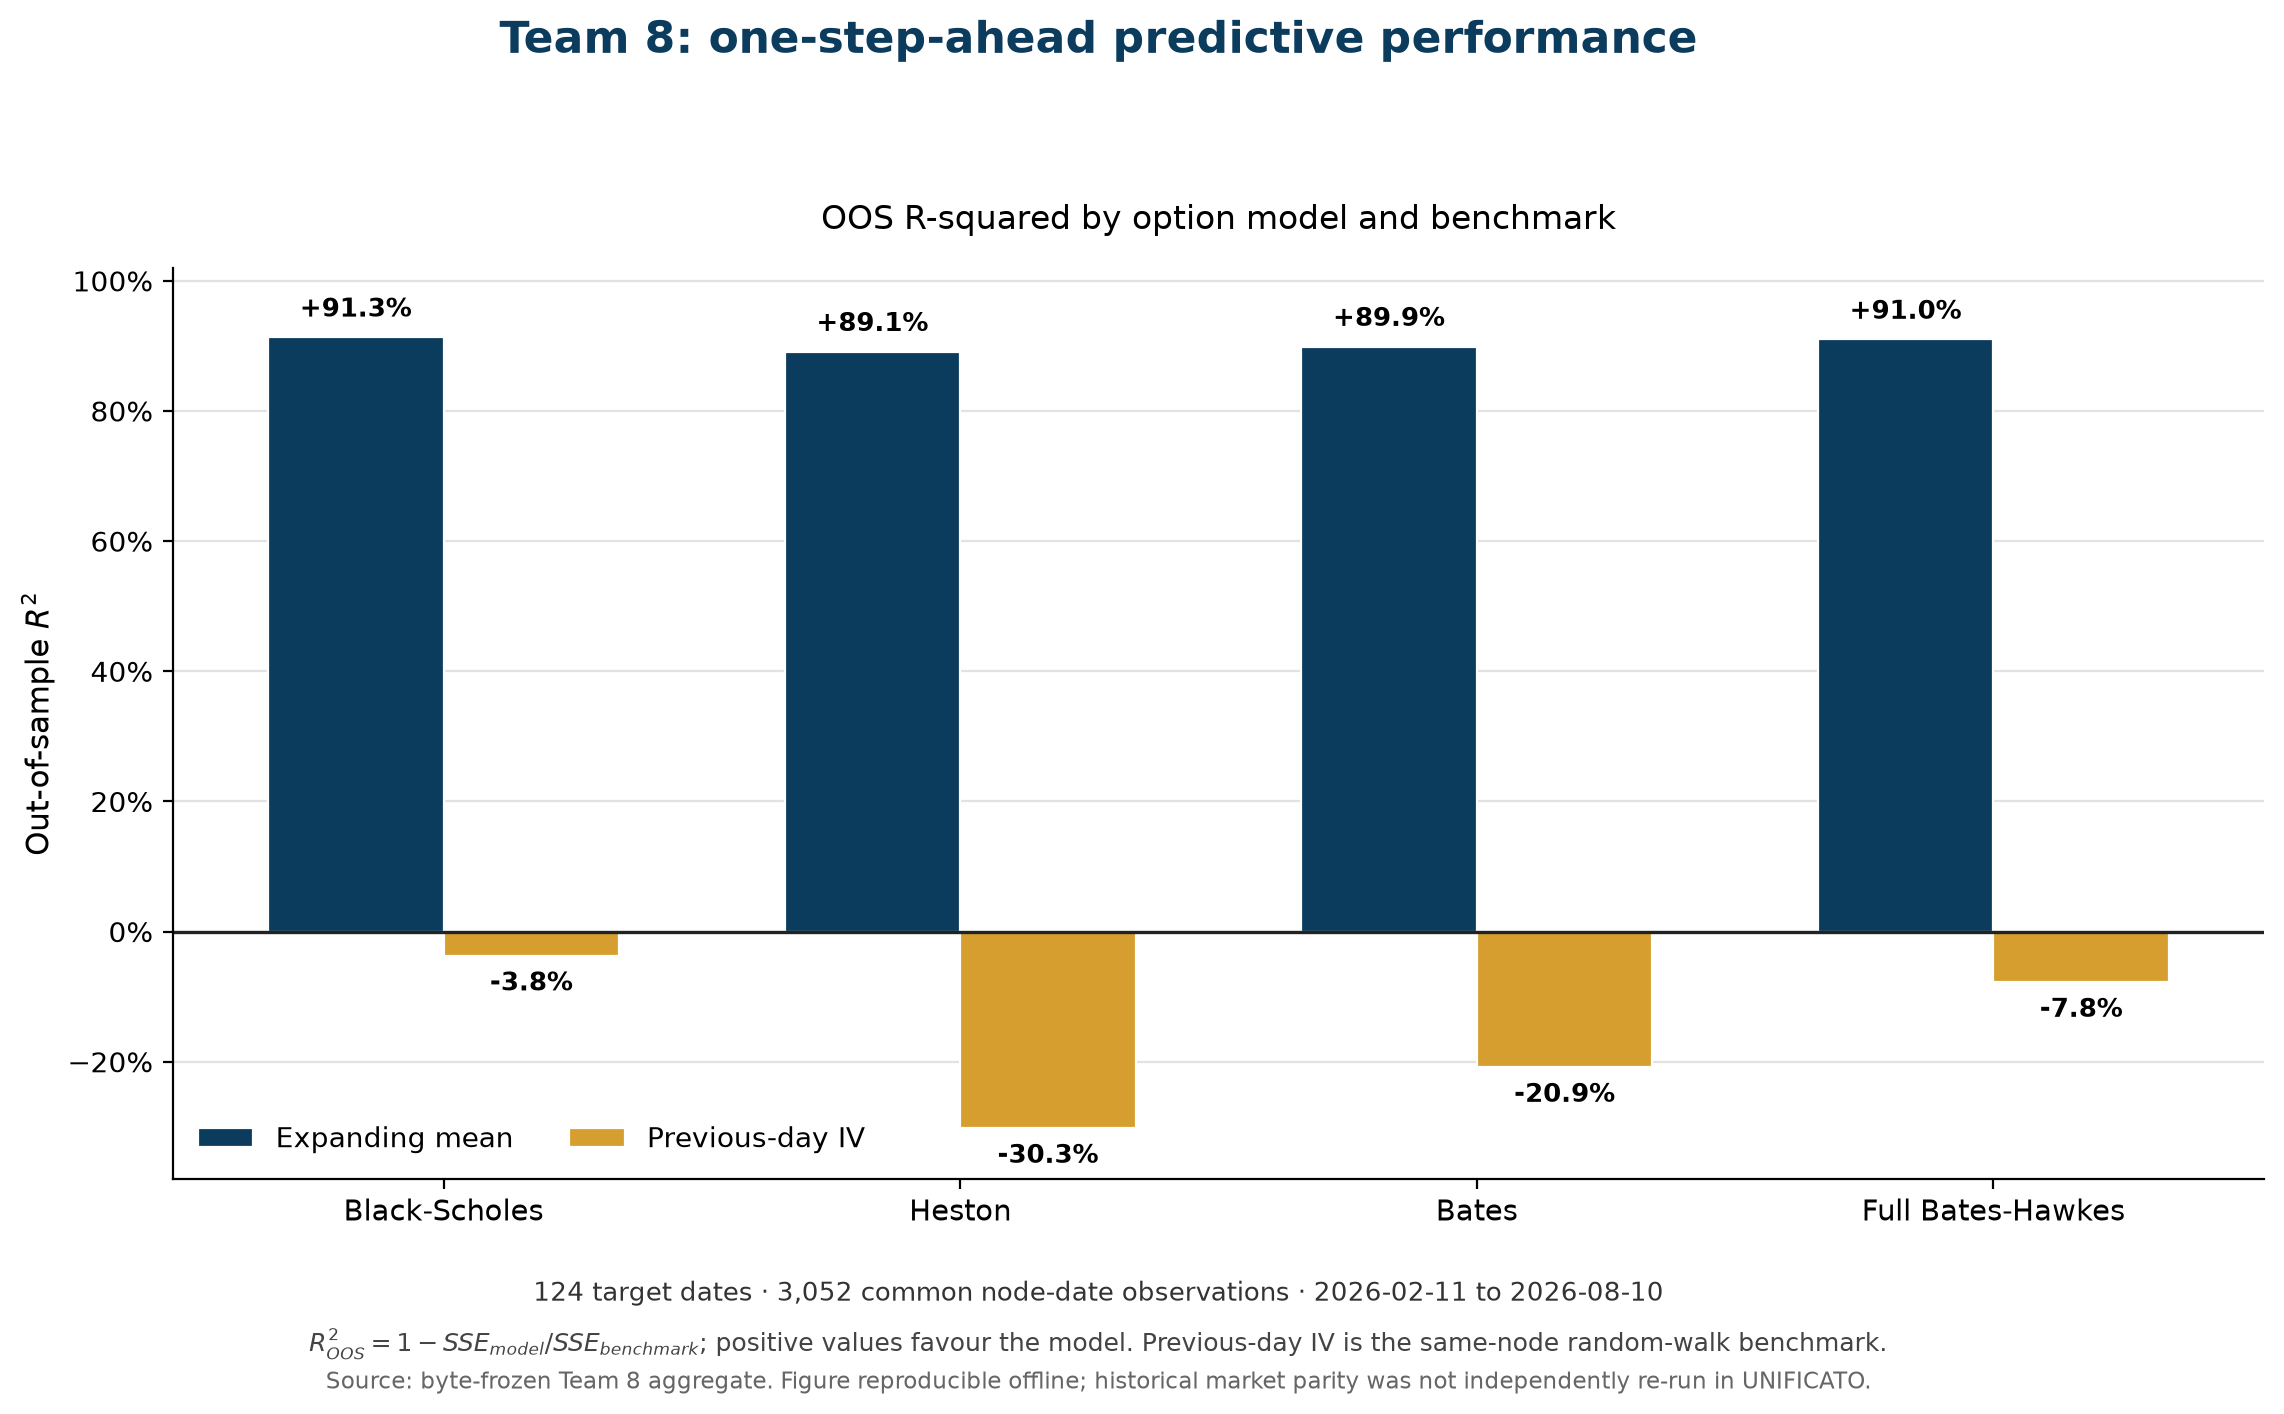
\includegraphics[width=0.98\textwidth]{img/diagnostics/online_oos_r2_by_benchmark.png}
    \caption{Team 8 rolling one-step-ahead out-of-sample \(R^2\) by model and
    benchmark. All four specifications improve on the node-specific expanding
    mean, but none improves on carrying forward the previous day's normalized
    IV surface. The chart is rebuilt offline from the byte-frozen aggregate;
    it does not claim independent historical market-parity replication.}
    \label{fig:online-oos-r2}
\end{figure}
}{%
\gapbox{The Team 8 OOS \(R^2\) chart is withheld unless it is regenerated from
the frozen online-validation metrics and passes the sample and identity checks.}%
}

All four models beat the expanding mean, and the HAC differences are significant. The stronger random-walk benchmark reverses the conclusion: no model has positive \(R^2_{OOS}\) against yesterday's surface. Black--Scholes has the lowest pooled RMSE, while full Bates--Hawkes is close; their pairwise \(R^2\) favors Black--Scholes by 3.77\%, but the HAC difference is not significant (\(p=0.421\)). Full Bates--Hawkes beats Heston by 17.23\% pairwise and the difference is systematic (\(p=1.06\times10^{-4}\)); its 10.81\% advantage over Bates is not significant (\(p=0.126\)). Thus added structure helps some comparisons, but daily IV persistence remains the hardest benchmark.

Rolling parameters also expose identification pressure. The full model's branching ratio has a median of 0.0203, close to the imposed 0.02 floor, and some jump-size parameters approach lower bounds. The current cross-section estimates stronger self-excitation, but the online history does not support presenting that current estimate as a stable law.
\subsubsection{Fixed-Cutoff Six-Month Stress Test}

The earlier frozen-parameter design is retained as a deliberately harsher robustness check, not as the primary online test. Parameters are estimated once on 10 February 2026 and never refitted during 27 weekly holdout surfaces through 10 August. Against the prevailing mean, \(R^2_{OOS}\) is 46.48\% for Black--Scholes, 44.60\% for Heston, 45.08\% for Bates, and 52.41\% for full Bates--Hawkes. The full model has the lowest frozen-parameter RMSE and significantly lower weekly loss than Heston and Bates, but not Black--Scholes. This stress result measures six-month parameter stability; it does not replace the current-snapshot calibration used by the controlled Barrick comparison.


% ===============================

The preceding model chapters described calibration, constraints, residuals, and smile slices in one place. This chapter checks whether those calibrated models behave sensibly on the option surface. It therefore collects the residual heatmaps, smile fits, and Bates--Hawkes visual diagnostics after the scalar model comparison has already been reported.
\subsection{What the Diagnostics Say Operationally}

The diagnostic layer should be read as a quality-control stage:

\begin{itemize}[leftmargin=8mm, itemsep=2pt]
    \item \textbf{Surface plots} show the empirical object being fitted.
    \item \textbf{Sampling plots} show which market observations are used for calibration and interpolation tests.
    \item \textbf{Residual heatmaps} show whether errors are random-looking or structurally concentrated.
    \item \textbf{Smile slices} show whether the fitted model has a plausible shape within each maturity bucket.
\end{itemize}

% Team 8 evidence regenerated by the unified branch. The rolling OOS figure is
% rendered from a frozen aggregate CSV because licensed option bars are local-only.

\subsubsection{Regenerated market-input and return evidence}

The scalar calibration errors reported above are interpretable only together
with the empirical objects that generated them. Figure~\ref{fig:t8-market-inputs}
shows the dated Treasury proxy and the structured option sample rebuilt by the
unified branch from the 2 September 2026 Team 8 snapshot. The raw licensed rows
remain local and Git-ignored; the figures and aggregate calibration outputs
carry hashes in the code-run manifest.

\begin{figure}[H]
    \centering
    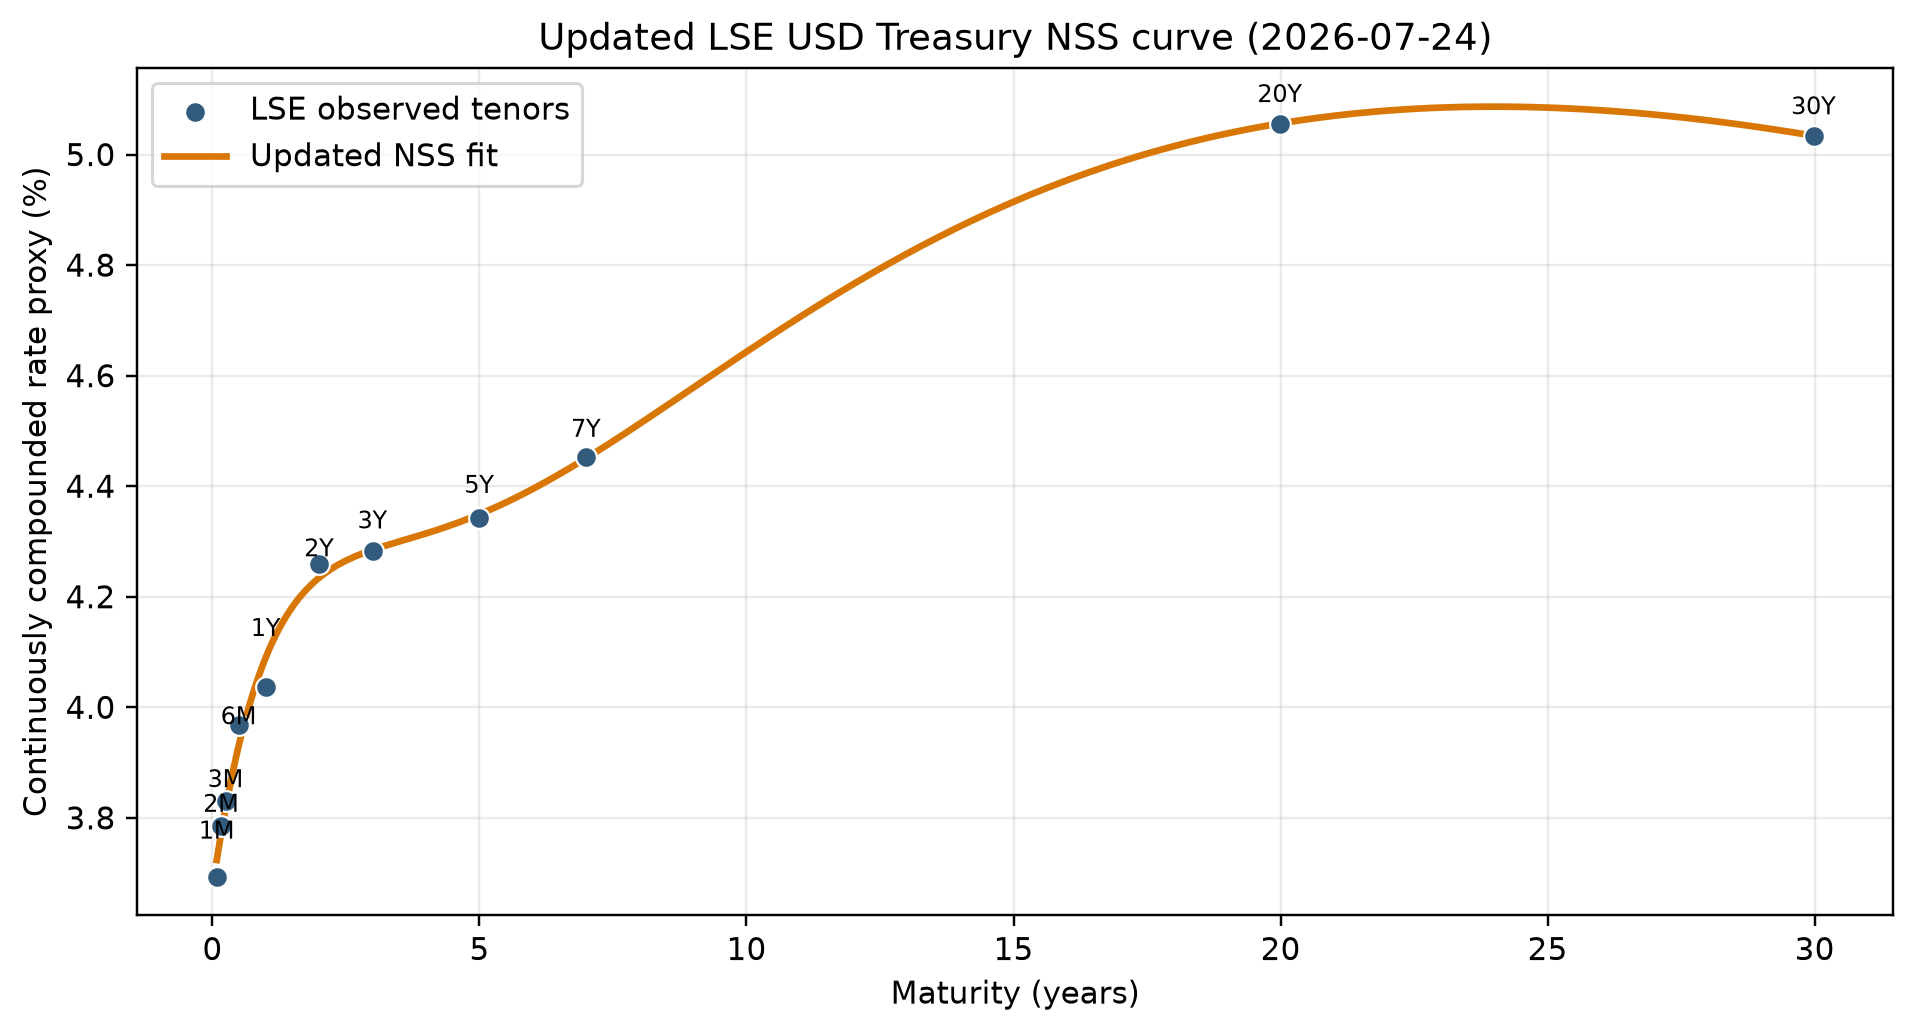
\includegraphics[width=0.82\textwidth]{img/team8_empirical/usd_treasury_curve.png}

    \vspace{4mm}
    
\includegraphics[width=0.88\textwidth]{img/team8_empirical/sampling_comparison.png}
    \caption{Team 8 calibration inputs. Top: 14 same-date continuously compounded U.S. Treasury proxies and their NSS fit
on 2 September 2026. Bottom: the CC64 sample selected from 605 eligible GLD calls
across 12 expiries and 146 strikes; the retained contracts span eight expiries
and 20 strikes. The colours encode observed
    implied volatility; the node layout, rather than an interpolated sheet,
    is the actual object passed to the optimizer.}
    \label{fig:t8-market-inputs}
\end{figure}

The historical GLD return series supplies a different diagnostic from the
option cross-section. It is observed under the historical data-generating
process and is used only to test Gaussian adequacy, not to estimate a physical
drift or to rank option-pricing models. Figure~\ref{fig:t8-return-normality}
shows both the central concentration and the tail departures that motivate a
variance-and-jump model stack.

\begin{figure}[H]
    \centering
    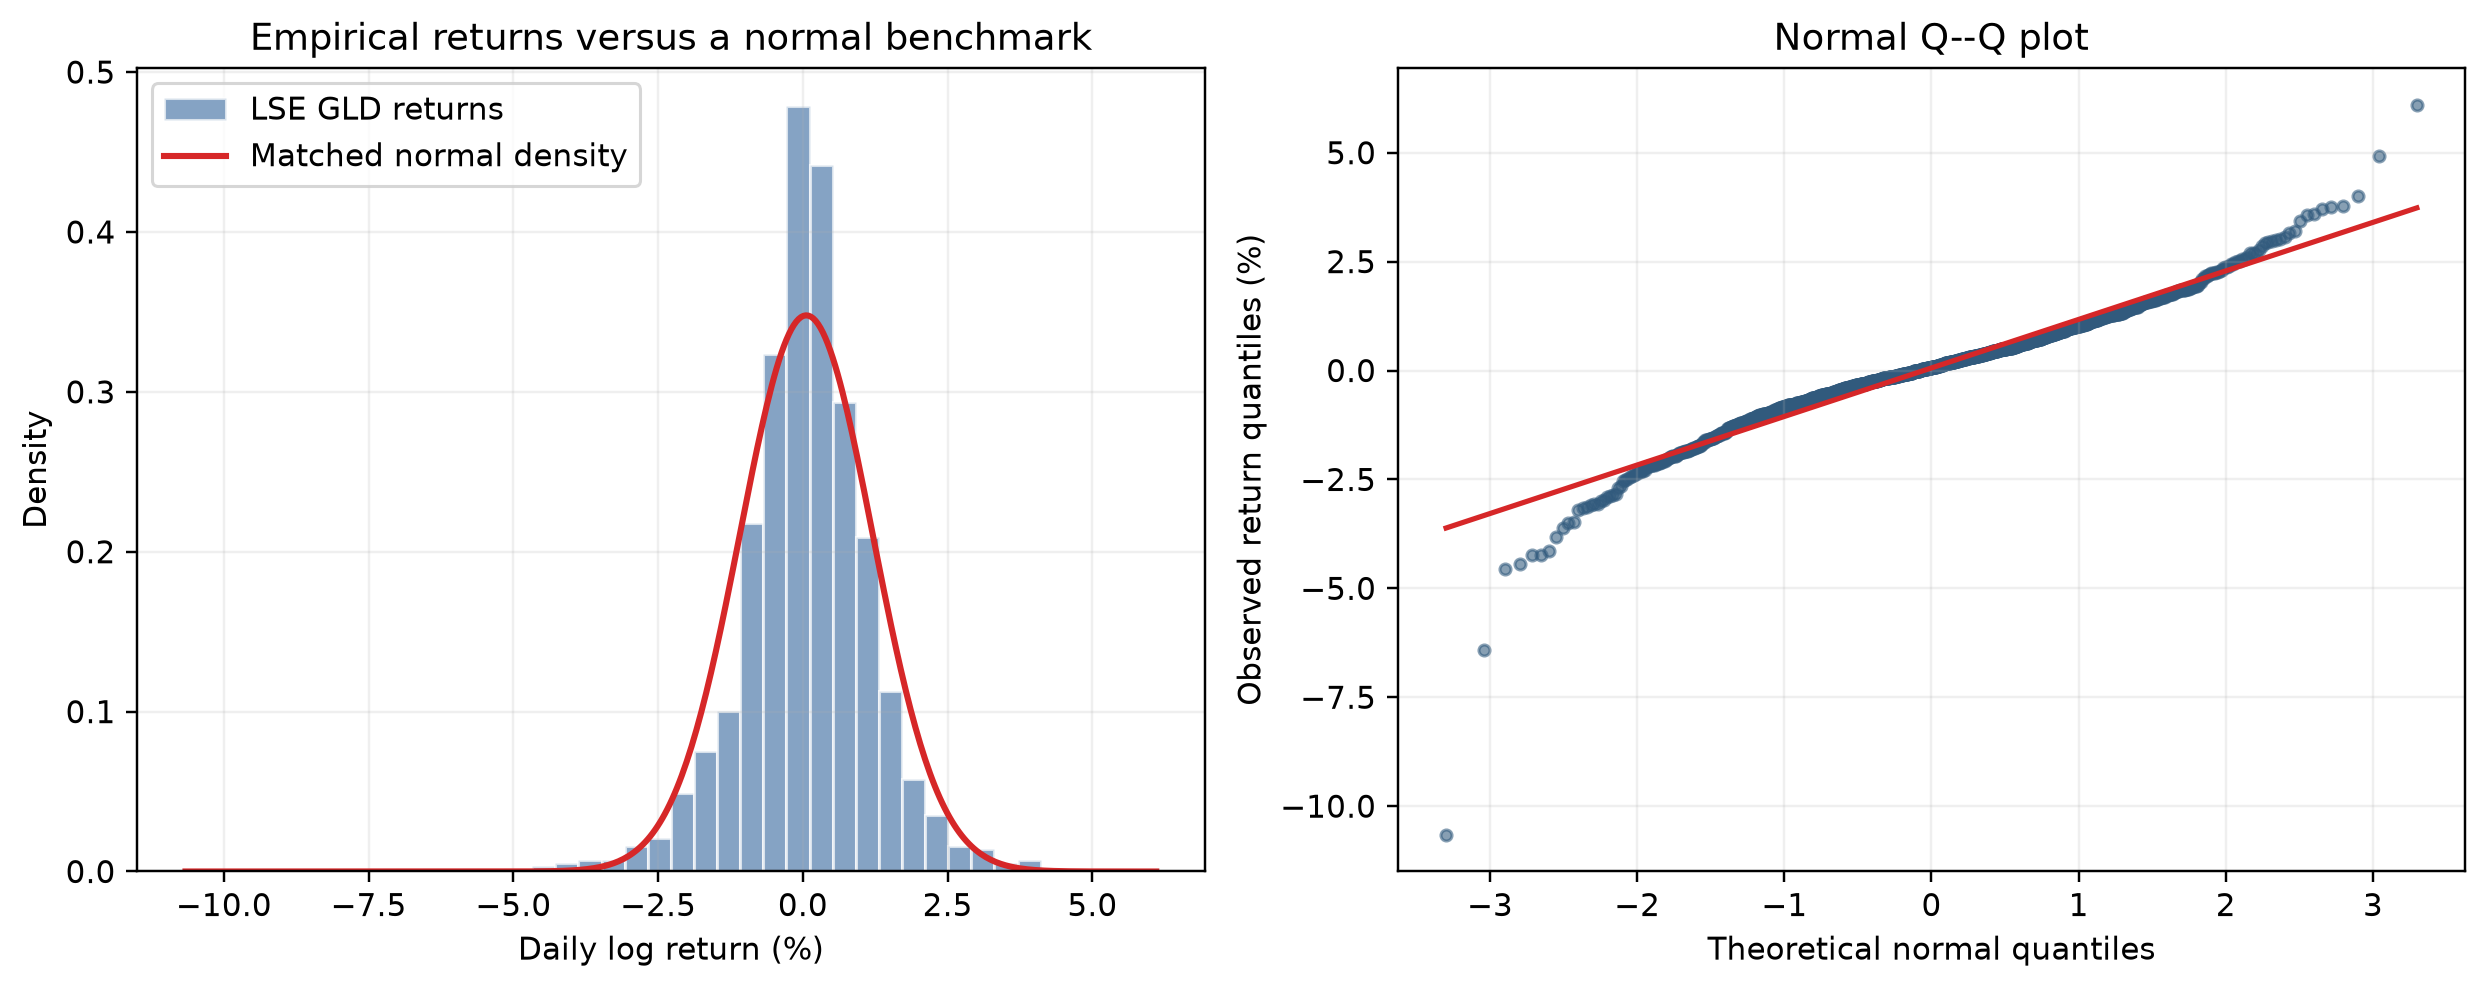
\includegraphics[width=0.96\textwidth]{img/team8_empirical/gld_return_normality.png}
    \caption{LSE GLD daily log returns from 5 January 2021 to 27 August 2026:
    empirical density against a matched normal law and normal Q--Q plot. The
    sample contains 1,424 observations; the visible tail departures are
    consistent with the formal tests in Table~\ref{tab:t8-return-normality}.}
    \label{fig:t8-return-normality}
\end{figure}

\begin{table}[H]
\centering
\footnotesize
\begin{tabular}{@{}lrrl@{}}
\toprule
Test & Statistic & \(p\)-value & Decision at 5\% \\
\midrule
Shapiro--Wilk & 0.9434 & \(6.25\cdot10^{-23}\) & Reject normality \\
Jarque--Bera & 3499.31 & \(<10^{-300}\) & Reject normality \\
D'Agostino \(K^2\) & 322.83 & \(7.90\cdot10^{-71}\) & Reject normality \\
\bottomrule
\end{tabular}
\caption{Normality tests for the 1,424 daily GLD log returns. Sample skewness
is \(-0.733\) and excess kurtosis is \(7.570\). Rejection motivates richer
dynamics but does not by itself select Heston, Bates or Bates--Hawkes.}
\label{tab:t8-return-normality}
\end{table}

\subsubsection{Cross-sectional calibration geometry}

Tables~\ref{tab:t8-model-parameters}--\ref{tab:t8-model-errors} consolidate
the point-in-time fit that is otherwise distributed across the model-specific
sections. All four rows use the same 64 actual nodes, price/IV conversion and
vega-weighted objective; richer models therefore change the state law rather
than the empirical target.

\begin{table}[H]
\centering
\scriptsize
\setlength{\tabcolsep}{2.6pt}
\begin{tabularx}{\textwidth}{@{}>{\RaggedRight\arraybackslash}p{2.35cm}>{\RaggedRight\arraybackslash}X>{\RaggedRight\arraybackslash}p{2.75cm}@{}}
\toprule
Model & Calibrated parameters & Admissibility \\
\midrule
Black--Scholes & \(\sigma=0.25088\). & Positive volatility. \\
Heston & \(v_0=0.06439,\; \kappa=4.05183,\; \theta_v=0.06548,\; \xi=0.72815,\; \rho=-0.01701\). & Feller gap 0.00043. \\
Bates--Poisson & \(v_0=0.06626,\; \kappa=4.05261,\; \theta_v=0.06324,\; \xi=0.67235,\; \rho=-0.03326,\; \lambda=0.24501,\; \mu_J=-0.02767,\; \sigma_J=0.00483\). & Feller gap 0.06053. \\
Full Bates--Hawkes & \(v_0=0.06514,\; \kappa=4.05259,\; \theta_v=0.06346,\; \xi=0.67263,\; \rho=-0.03322,\; \lambda_0=0.03496,\; \bar\lambda=0.56005,\; n=0.55690,\; \beta=2.74823,\; \mu_J=-0.02901,\; \sigma_J=0.02280\). & Feller gap 0.06196; stationary $n<1$. \\
\bottomrule
\end{tabularx}
\caption{Feller-constrained parameters on the current 2 September 2026 Team 8 Chebyshev sample.}
\label{tab:t8-model-parameters}
\end{table}

\begin{table}[H]
\centering
\scriptsize
\setlength{\tabcolsep}{3.1pt}
\begin{tabularx}{\textwidth}{@{}>{\RaggedRight\arraybackslash}p{2.35cm}rrrr>{\RaggedRight\arraybackslash}X@{}}
\toprule
Model & Price MAE & Price RMSE & IV MAE bp & IV RMSE bp & Reading \\
\midrule
Black--Scholes & 0.699 & 0.832 & 73.06 & 97.21 & Common CC64 target. \\
Heston & 0.398 & 0.501 & 38.48 & 49.49 & Lowest current in-sample error. \\
Bates--Poisson & 0.447 & 0.562 & 42.60 & 54.63 & Common CC64 target. \\
Full Bates--Hawkes & 0.410 & 0.514 & 40.76 & 52.97 & Common CC64 target. \\
\bottomrule
\end{tabularx}
\caption{Calibration errors on a common option sample. Heston has the lowest
in-sample IV RMSE; this cross-sectional fit is not an out-of-sample ranking.}
\label{tab:t8-model-errors}
\end{table}

The Full Bates--Hawkes branching ratio is 0.5569, below unity and away from
the former lower bound. This snapshot permits material self-excitation, but
does not establish stable identification across regimes. Heston remains the
current-fit winner; Hawkes is selected separately on rolling OOS performance.

The residual maps in Figures~\ref{fig:t8-residual-atlas-diffusion} and
\ref{fig:t8-residual-atlas-jumps} restore the spatial information hidden by
one RMSE. The continuous colours are interpolation only inside the observed
node domain; the circles identify the observations. Their purpose is to show
where errors remain systematic across maturity and moneyness.

\begin{figure}[p]
    \centering
    
\includegraphics[width=0.49\textwidth]{img/team8_empirical/black_scholes_residual_heatmap.png}\hfill
    
\includegraphics[width=0.49\textwidth]{img/team8_empirical/heston_residual_heatmap.png}
    \caption{Market-minus-model implied-volatility residuals for the two
    diffusion specifications: Black--Scholes (left) and Feller-constrained
    Heston (right). Stochastic variance reduces the scalar loss but does not
    remove structured maturity--moneyness error.}
    \label{fig:t8-residual-atlas-diffusion}
\end{figure}

\begin{figure}[p]
    \centering
    
\includegraphics[width=0.49\textwidth]{img/team8_empirical/bates_residual_heatmap.png}\hfill
    
\includegraphics[width=0.49\textwidth]{img/team8_empirical/bates_hawkes_residual_heatmap.png}
    \caption{Market-minus-model implied-volatility residuals after adding
    discontinuities: Bates--Poisson (left) and Full Bates--Hawkes (right).
    The Hawkes layer lowers the current scalar error, while visible clusters
    remain and residual normality is still rejected.}
    \label{fig:t8-residual-atlas-jumps}
\end{figure}

\begin{figure}[p]
    \centering
    
\includegraphics[width=0.97\textwidth]{img/team8_empirical/bates_hawkes_volatility_smile.png}
    \caption{Observed and Full Bates--Hawkes implied-volatility smiles across
    the eight sampled expiries. The panel view prevents a low aggregate RMSE
    from concealing expiry-specific misses, especially at boundary strikes.}
    \label{fig:t8-bh-smiles}
\end{figure}

The standalone study also compared three Hawkes routes that estimate
different objects. Table~\ref{tab:t8-hawkes-routes} preserves that distinction:
event-time likelihoods are kernel diagnostics, whereas only an option-price
calibration can enter the like-for-like surface comparison.

\begin{table}[H]
\centering
\scriptsize
\setlength{\tabcolsep}{3pt}
\begin{tabularx}{\textwidth}{@{}p{2.25cm}p{2.55cm}p{3.45cm}X@{}}
\toprule
Route & Target & Frozen result & Role \\
\midrule
Exact constant-volatility Hawkes & GLD option surface & \(\sigma=0.22448\),
\(n=0.00460\), objective \(8.674\cdot10^{-5}\). & Transform benchmark;
excludes the Heston variance state. \\
Exponential kernel & Event times & \(n=0.3884\), log-likelihood \(-67.75\),
AIC 141.51, BIC 147.36. & Stable Markovian kernel compatible with affine
pricing. \\
Rough power-law kernel & Event times & \(n=0.4119\), log-likelihood \(-68.03\),
AIC 144.05, BIC 151.86. & Long-memory diagnostic; not the option-pricing
model used in the comparison. \\
\bottomrule
\end{tabularx}
\caption{Historical source-study Hawkes routes; these frozen estimates are not the current September parameter set.}
\label{tab:t8-hawkes-routes}
\end{table}

\begin{figure}[p]
    \centering
    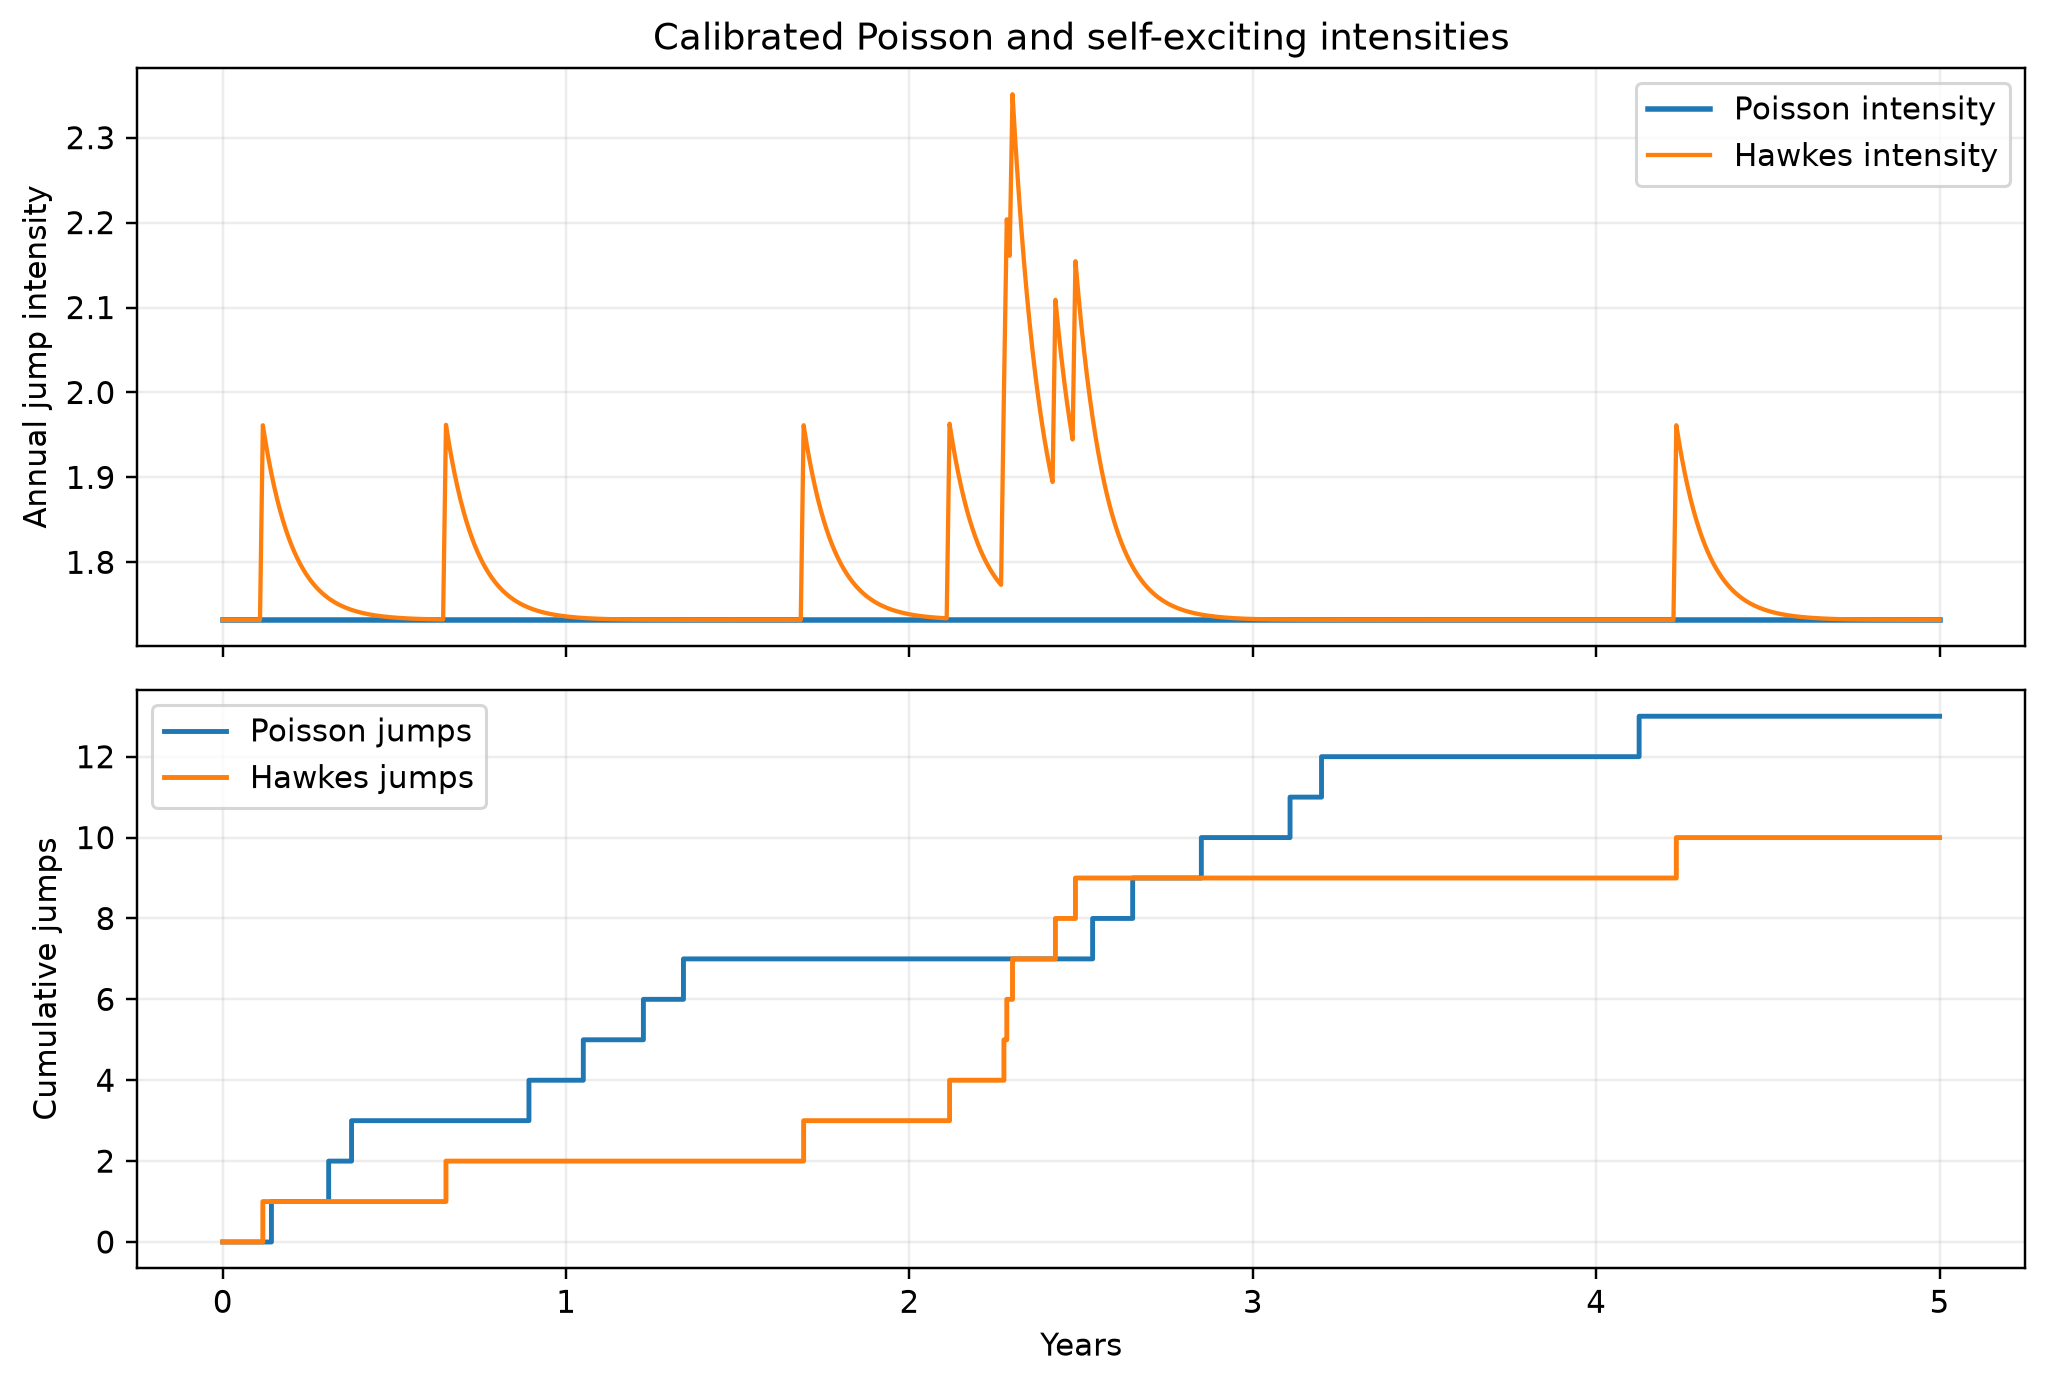
\includegraphics[width=0.94\textwidth]{img/team8_empirical/hawkes_intensity_comparison.png}
    \caption{Constant-intensity Bates jumps versus self-exciting
    Bates--Hawkes jumps regenerated from the current calibration. A Hawkes arrival raises
    near-term intensity, which subsequently decays toward its baseline; the
    lower panel shows the associated clustered event counts.}
    \label{fig:t8-hawkes-intensity}
\end{figure}

\begin{figure}[p]
    \centering
    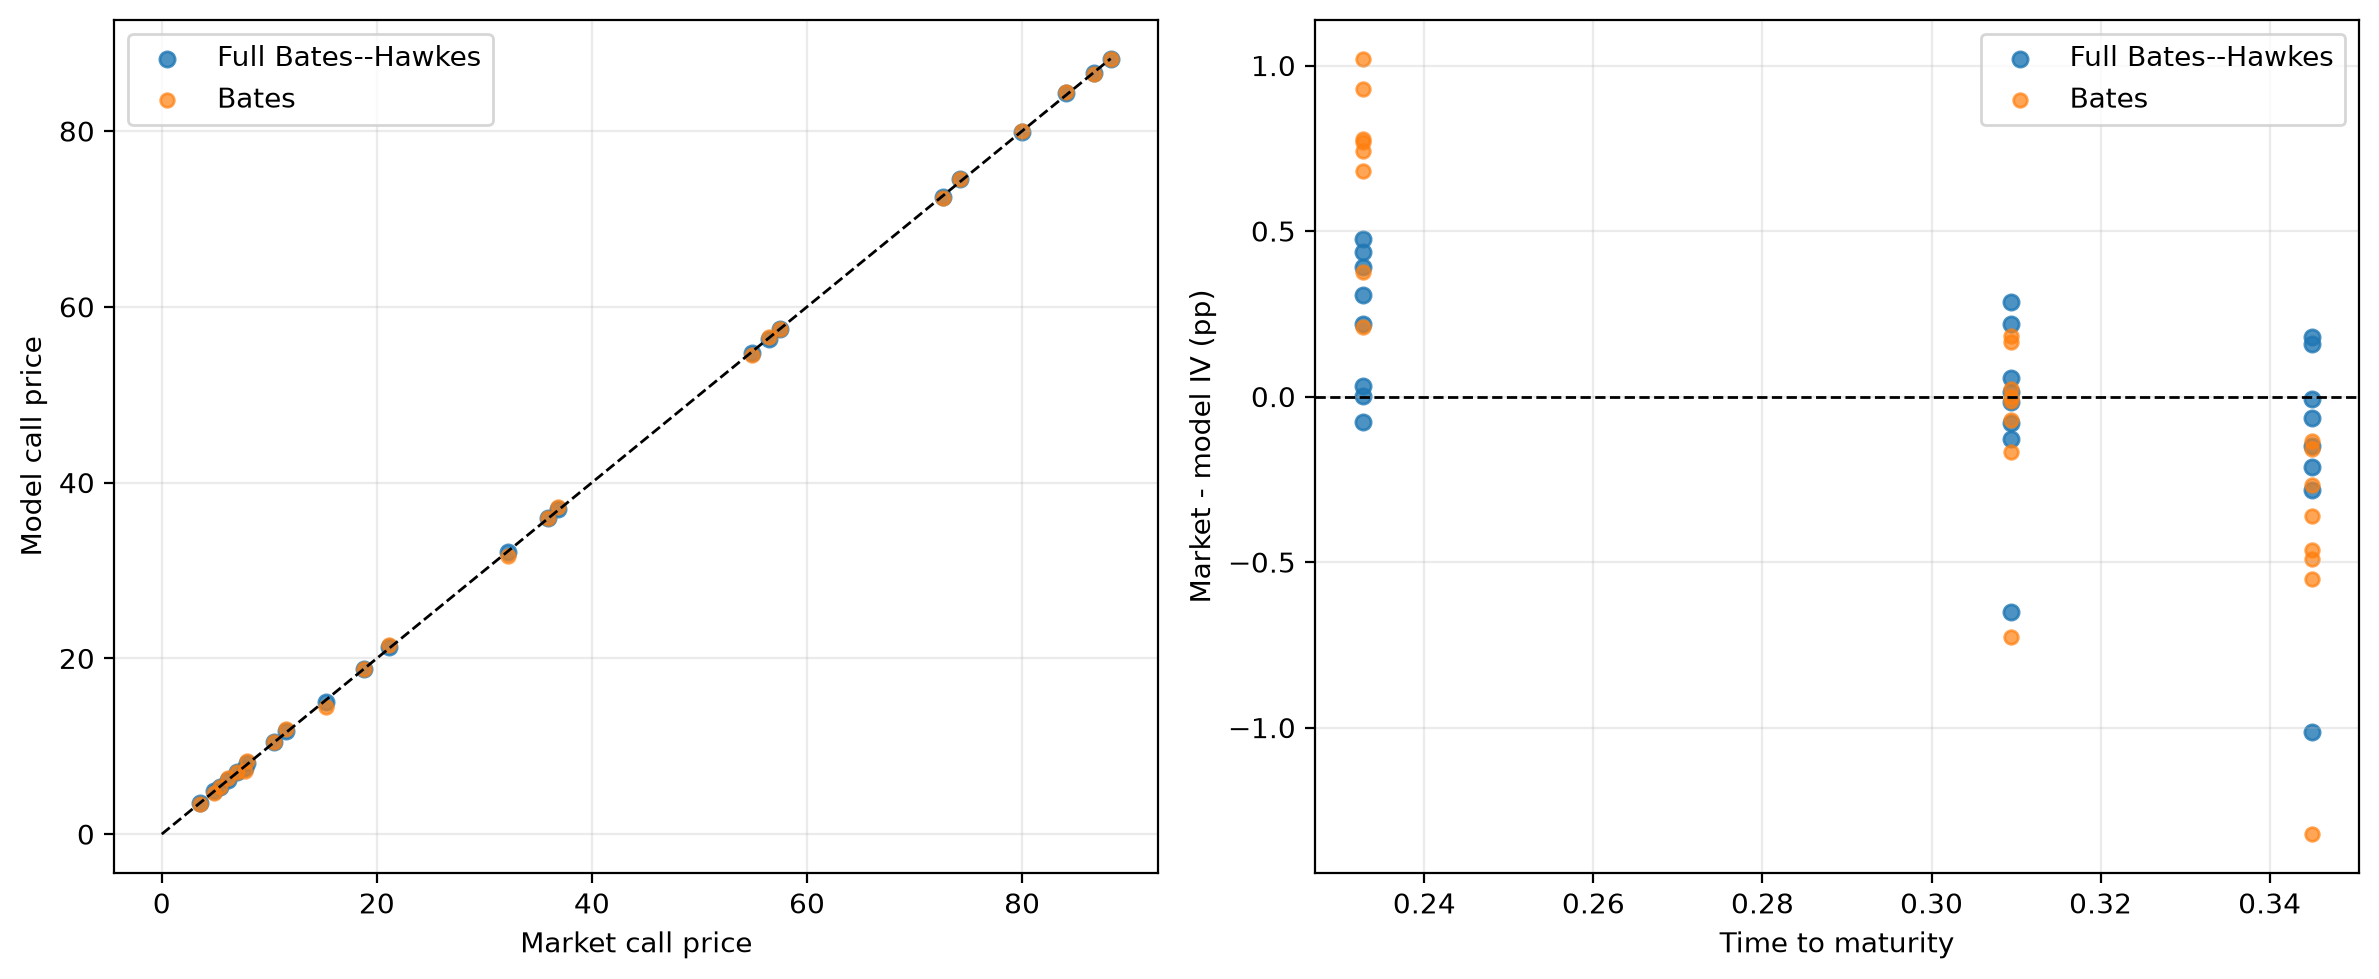
\includegraphics[width=0.98\textwidth]{img/team8_empirical/bates_hawkes_vs_bates.png}
    \caption{Direct current-snapshot comparison between Full Bates--Hawkes and
    Bates--Poisson. The left panel checks option prices against the diagonal;
    the right panel compares market-minus-model IV residuals by maturity. This
    is cross-sectional fit evidence, not proof of predictive dominance.}
    \label{fig:t8-bh-versus-bates}
\end{figure}

\subsubsection{Chronological loss accumulation}

Figure~\ref{fig:t8-welch-goyal} displays the September dense-only rolling
loss differences. The benchmark is the origin cross-sectional mean IV or the
interpolated origin IV surface. Black--Scholes does not beat the mean benchmark;
the three richer models do, but none beats persistence. Full Bates--Hawkes has
the lowest date-equal IV RMSE among the four candidates. These benchmark
comparisons do not establish physical gold forecasting accuracy.

\begin{figure}[p]
    \centering
    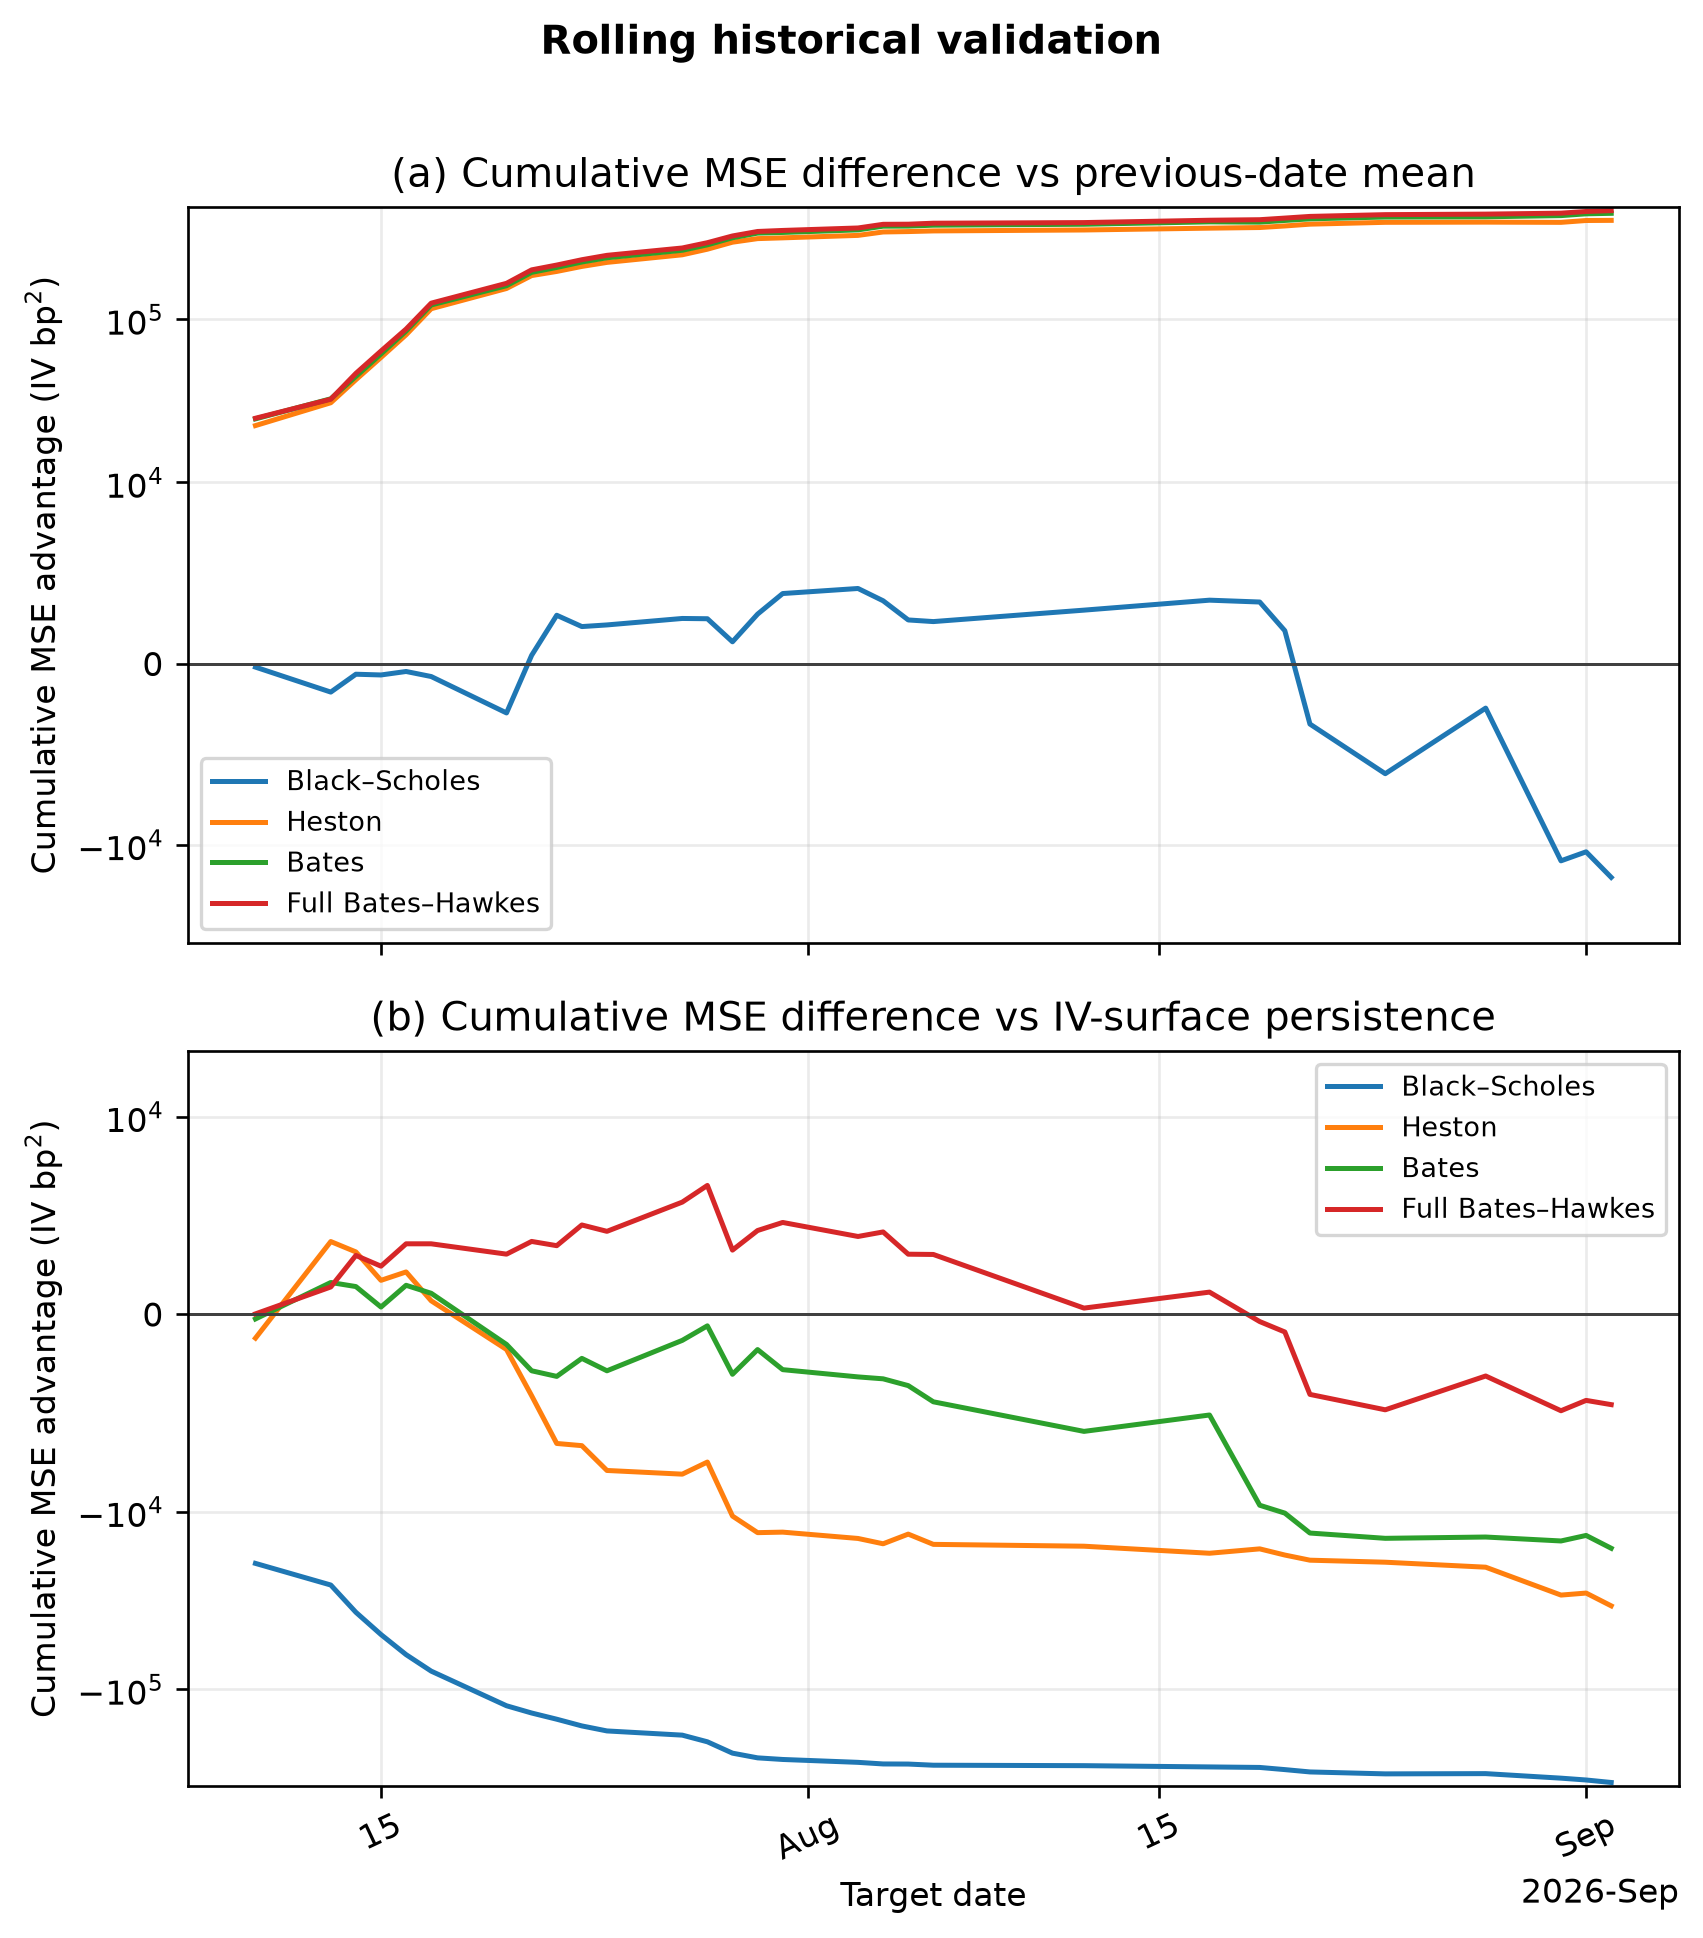
\includegraphics[width=0.98\textwidth]{img/team8_empirical/online_welch_goyal_cumulative.png}
    \caption{Dense-only rolling one-step-ahead Welch--Goyal cumulative squared-error
    differences over the Team 8 validation window, freshly rendered from
    aggregate outputs. Upward movement favours
    the named model relative to the comparator in each panel. The time path
    explains why a positive comparison with the origin mean coexists with
    failure against yesterday's observed IV surface.}
    \label{fig:t8-welch-goyal}
\end{figure}


This is why the article emphasizes diagnostics rather than only model formulas. In applied quantitative finance, a calibrated parameter vector is not self-validating. The model must be checked against the geometry of the observed surface, the admissibility of the parameters, and the stability of the numerical routine. These checks prepare the final step: translating calibrated parameters into simulated gold-price paths.

% ===============================
\subsection{From Calibrated Options to Gold-Price Paths}

Previous work in this track shows why Monte Carlo is the natural numerical language for path-dependent risk and valuation problems, following the same simulation logic developed in standard references such as Glasserman \sourcecitation{Glasserman2003,BarrickArticle3}. Once a stochastic law is specified, many scenarios can be generated and the resulting distribution can be summarized through percentiles, confidence intervals, VaR, CVaR, or other functionals. Earlier company-level modelling also shows why a Barrick framework needs gold-price scenarios. This Team 8 module stops at construction and testing of the price process; Chapter~12 performs the separate corporate integration \sourcecitation{BarrickArticle4,BarrickArticle5}.

The present chapter supplies the price-model block only. In the earlier scenario exercise, a GBM was driven by a Black--Scholes-implied volatility term structure \sourcecitation{BarrickArticle4}. That choice was coherent as a first benchmark, but it inherits the limitations of Black--Scholes: lognormal continuous paths, no stochastic volatility, no jump risk, and no endogenous volatility smile. Heston and Bates provide two natural upgrades because they can be calibrated to the option surface rather than only to a per-maturity scalar volatility.

The simulation layer can reuse the numerical improvements developed in previous Monte Carlo work \sourcecitation{BarrickArticle3}, but it should not repeat that article's comparison between pseudo-random Monte Carlo, quasi Monte Carlo, antithetic variates, and moment matching. Here those tools are inputs. The applied question is different: once a calibrated gold-price law has been chosen, which simulation map is coherent with its state variables?

The accepted implementation uses one Sobol-based simulation interface with moment matching, aligned base seeds and model-specific transformations, while exposing separate policies for diffusion and event-driven blocks. A GBM path needs one Brownian shock, whereas a Bates--Hawkes path needs diffusive shocks, stochastic variance, jump marks and a self-exciting arrival mechanism. The completed design therefore shares what is comparable without pretending that all four models have the same random structure.

% Asset/code block omitted pending provenance acceptance.
\subsection{Monte Carlo Discretization by Model}

The equations below define the implemented model updates. The sampling policy is passed as a simulation configuration rather than hidden inside the financial model itself.

For the GBM baseline, a discrete gold-price update is
\begin{equation}
    S_{t+\Delta t}
    =
    S_t
    \exp\left[
        \left(r_t-q-\frac{1}{2}\sigma_t^2\right)\Delta t
        + \sigma_t\sqrt{\Delta t}\,Z_t
    \right],
\end{equation}
where \(\sigma_t\) is obtained from the Black--Scholes implied-volatility extraction. This is an efficient first approximation, but it compresses the whole option smile into one volatility input per maturity.

For Heston, the Monte Carlo engine simulates both price and variance. Its full-truncation Euler scheme is
\begin{align}
    v_{t+\Delta t}
    &=
    \max\left(
        v_t + \kappa(\theta_v-\max(v_t,0))\Delta t
        + \xi\sqrt{\max(v_t,0)}\sqrt{\Delta t}\,Z_t^v,
        0
    \right),\\
    S_{t+\Delta t}
    &=
    S_t
    \exp\left[
        \left(r_t-q-\frac{1}{2}\max(v_t,0)\right)\Delta t
        + \sqrt{\max(v_t,0)}\sqrt{\Delta t}\,Z_t^S
    \right],
\end{align}
with \(\operatorname{corr}(Z_t^S,Z_t^v)=\rho\). In this version, volatility is no longer an exogenous deterministic curve: it is a simulated state variable calibrated to option prices.

For Bates, the Heston price update receives an additional jump component:
\begin{equation}
    S_{t+\Delta t}
    =
    S_t
    \exp\left[
        \left(r_t-q-\lambda k-\frac{1}{2}\max(v_t,0)\right)\Delta t
        + \sqrt{\max(v_t,0)}\sqrt{\Delta t}\,Z_t^S
        + \sum_{j=1}^{N_t} J_{t,j}
    \right],
\end{equation}
where \(N_t\sim\operatorname{Poisson}(\lambda\Delta t)\), \(J_{t,j}\sim\mathcal{N}(\mu_J,\sigma_J^2)\), and \(k=\exp(\mu_J+\frac{1}{2}\sigma_J^2)-1\). This is the simulation counterpart of the Fourier-pricing model calibrated in the preceding sections. The implemented diffusion block uses moment-matched scrambled Sobol normals; jump counts use an inverse Poisson transform and jump marks use a separate normal block.

\paragraph{Bates--Hawkes extension.}
The Bates--Hawkes model keeps the Heston variance update and replaces the constant jump intensity \(\lambda\) by a stochastic self-exciting intensity,
\[
    \lambda_t = \bar{\lambda}+(\lambda_0-\bar{\lambda})e^{-\beta t}+\sum_{t_i<t}\alpha e^{-\beta(t-t_i)},
\]
so that recent jumps increase near-term jump probability while variance remains stochastic. Event times are simulated by Ogata thinning, the integrated intensity supplies the risk-neutral jump compensator over each time step, and the same full-truncation Heston update used by Bates evolves \(v_t\). The resulting process is therefore a genuine Bates--Hawkes path model, not an exact-Hawkes jump layer attached to constant volatility.

Before the path figures, Table~\sourceref{tab:terminal-path-stats} records the terminal distribution diagnostics. The Bates--Hawkes row uses all parameters from the full call-price calibration in Chapter 6: Heston variance, separate initial and baseline intensities, self-excitation, and lognormal jump marks.

% Asset/code block omitted pending provenance acceptance.


\IfFileExists{img/diagnostics/terminal_return_percentiles.png}{%
% Asset/code block omitted pending provenance acceptance.

}{}

\subsection{Path Simulation Diagnostics}

The calibrated parameter sets are translated into simulated five-year gold-price paths. The Black--Scholes/GBM panel uses a constant implied-volatility input. Heston uses stochastic variance, Bates adds discontinuous Poisson jumps, and the full Bates--Hawkes panel combines a Heston variance process with event-driven self-exciting jump arrivals. All figures and terminal statistics in this section were regenerated after the final Feller-constrained calibration.

% Asset/code block omitted pending provenance acceptance.


\IfFileExists{img/valuation/gold_path_bands_four_models.png}{%
\begin{figure}[H]
    \centering
    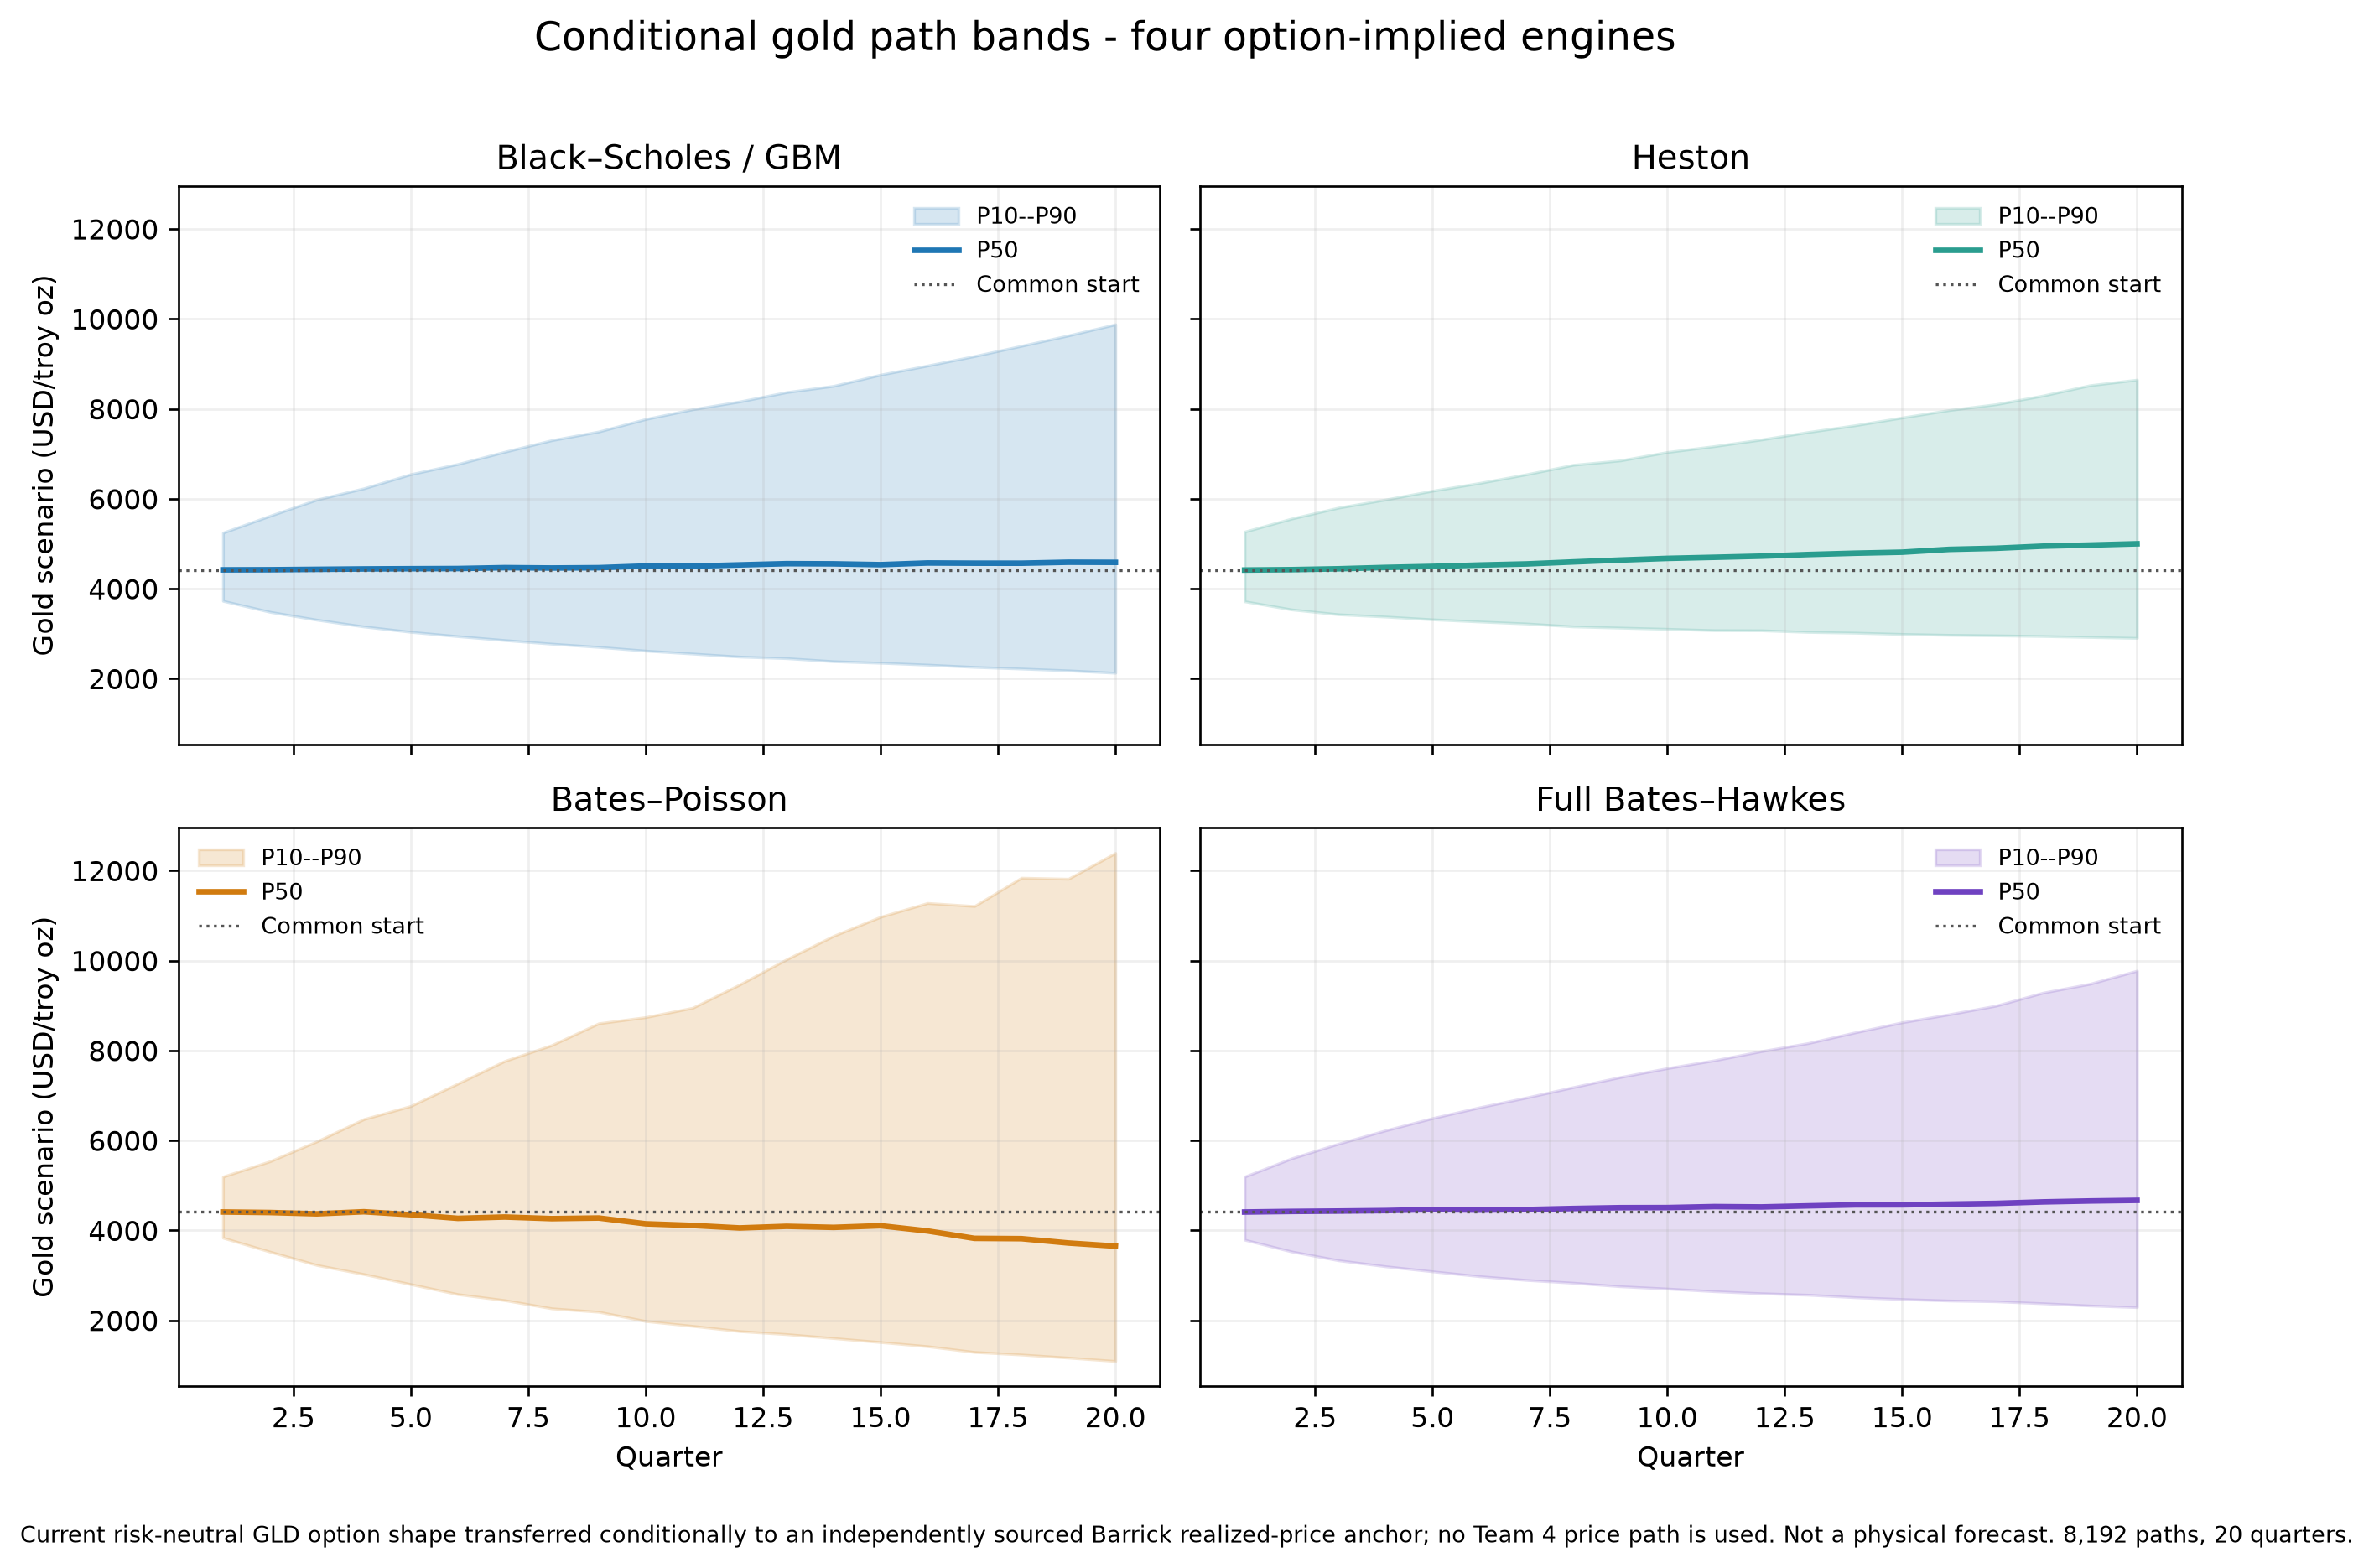
\includegraphics[width=0.98\textwidth]{img/valuation/gold_path_bands_four_models.png}
    \caption{Conditional P10--P50--P90 gold-path bands for Black--Scholes/GBM,
    Heston, Bates--Poisson and Full Bates--Hawkes. The 8,192 paths share the
    common Barrick Q2 2026 realised-price anchor of USD 4,417/troy oz, a
    five-year/20-quarter horizon and aligned base seeds. The option-implied
    shape comes from the current 27 August 2026 Team~8 calibration. Team~4
    price paths are not used. These are risk-neutral conditional scenarios, not a validated
    physical forecast or a Q-to-P mapping.}
    \label{fig:gold-path-bands-four-models}
\end{figure}
}{%
\gapbox{The four-model gold-path bands are withheld unless the accepted
CODE-012 figure bundle and its CSV/JSON sidecars are available.}%
}

The latent states are shown separately so their scales remain readable. Heston, Bates, and full Bates--Hawkes each carry stochastic variance. Bates has a constant annual Poisson intensity, whereas the Hawkes intensity jumps upward after arrivals and decays toward \(\bar{\lambda}\). Keeping volatility, Hawkes jumps, and Bates jumps in three figures avoids compressing a nearly constant intensity beside a much more variable volatility process.

% Selected simulation evidence regenerated by the unified branch.

\subsubsection{Current terminal distribution and latent-state diagnostics}

The current Team~8 diagnostic simulation uses the 2 September calibration,
4,096 paths, 260 steps and the GLD level 402.78 USD/share. Its constant
annual rate is 4.0770\%, as recorded in the diagnostic table. This standalone
state-law illustration differs from the corporate adapter, which restarts at
Barrick's realised-price anchor and uses integral-preserving NSS forward rates
and 8,192 paths. Neither the levels nor the path percentiles are interchangeable.

\begin{table}[H]
\centering
\scriptsize
\setlength{\tabcolsep}{2.45pt}
\begin{tabular}{@{}lrrrrrrrr@{}}
\toprule
Model & Mean & Std & P05 & P50 & P95 & Return skew & Ex. kurt. & Mean jumps \\
\midrule
GBM / BS & 490.549 & 289.852 & 160.071 & 423.839 & 1036.482 & 1.743 & 5.708 & 0.000 \\
Heston & 495.256 & 308.314 & 164.068 & 421.222 & 1087.352 & 2.133 & 9.293 & 0.000 \\
Bates & 496.912 & 310.039 & 161.053 & 421.499 & 1098.107 & 2.069 & 7.779 & 1.259 \\
Full Bates--Hawkes & 494.830 & 300.874 & 164.799 & 425.021 & 1063.213 & 1.901 & 6.477 & 5.206 \\
\bottomrule
\end{tabular}
\caption{Terminal GLD price and simple-return diagnostics regenerated from the
current Team 8 calibration: 4,096 five-year paths, 260 steps and a fixed seed. The jump
models mainly alter tail shape and event counts; these levels are not Barrick
values and are not inputs to the later 8,192-path corporate comparison.}
\label{tab:t8-terminal-path-stats}
\end{table}

\begin{figure}[p]
    \centering
    
\includegraphics[width=0.94\textwidth]{img/team8_empirical/terminal_return_percentiles.png}
    \caption{All integer percentiles 0--100 of five-year simple GLD returns in
    the current Team 8 simulation. The symmetric-log scale retains the
    central distribution while exposing extreme endpoints; the full integer
    percentile tables remain in the source article rather than being repeated
    in the thesis.}
    \label{fig:t8-terminal-return-percentiles}
\end{figure}

\begin{figure}[p]
    \centering
    
\includegraphics[width=0.98\textwidth]{img/team8_empirical/volatility_state_paths.png}
    \caption{Representative annualized stochastic-volatility paths under
    Heston, Bates and Full Bates--Hawkes on a common scale. The plot verifies
    that all three richer engines carry a simulated variance state; the jump
    mechanism does not replace stochastic variance.}
    \label{fig:t8-volatility-state-paths}
\end{figure}

\begin{figure}[p]
    \centering
    
\includegraphics[width=0.68\textwidth]{img/team8_empirical/bates_poisson_jump_paths.png}

    \vspace{3mm}
    
\includegraphics[width=0.68\textwidth]{img/team8_empirical/hawkes_jump_paths.png}
    \caption{Representative jump-state diagnostics. Top: Bates retains a
    constant Poisson intensity while cumulative counts evolve independently.
    Bottom: Full Bates--Hawkes intensity rises after arrivals and decays toward
    its baseline, generating clustered event counts. These path displays
    explain the state difference behind the tail comparison; they are not
    additional forecast observations.}
    \label{fig:t8-jump-state-comparison}
\end{figure}


\IfFileExists{img/diagnostics/volatility_state_paths.png}{%
% Asset/code block omitted pending provenance acceptance.

}{}

\IfFileExists{img/diagnostics/hawkes_jump_paths.png}{%
% Asset/code block omitted pending provenance acceptance.

}{}

\IfFileExists{img/diagnostics/bates_poisson_jump_paths.png}{%
% Asset/code block omitted pending provenance acceptance.

}{}
\subsection{Interface with the Unified Barrick Experiment}

The practical reason for introducing Heston, Bates, and the Bates--Hawkes extension is to provide a stronger gold-price input. This Team 8 module does not estimate Barrick revenues, EBITDA, cash flows or equity value by itself. Its output is narrower: calibrated parameters, option-surface diagnostics and simulated gold-price paths. Chapter~12 connects that output to the separate Team 4 operating layer and Team 5 corporate valuation contract.

The unified experiment connects those paths to production, costs and company-level valuation assumptions through a clean interface:
\[
    \left\{
    S_t^{(m)},\,
    v_t^{(m)},\,
    N_t^{(m)},\,
    \lambda_t^{(m)}
    \right\}_{t=0}^{T},
\]
where \(S_t^{(m)}\) is the simulated gold price, \(v_t^{(m)}\) is the variance path when the model has stochastic volatility, \(N_t^{(m)}\) is the jump count, and \(\lambda_t^{(m)}\) is the jump intensity for the Hawkes extension. The superscript \(m\) denotes the Monte Carlo path. Keeping this boundary explicit prevents the article from confusing two different tasks: modelling the gold price and mapping that price into corporate revenues and value.
\subsection{No Investment Recommendation}

The models in this chapter are research tools. They are used to study the shape of option prices, the numerical behaviour of calibration routines, and the possible distribution of model-driven gold-price paths. They do not provide a recommendation to buy, sell, or hold Barrick Gold, GLD, options, or any related financial instrument. A model-implied price, volatility, or path distribution is conditional on assumptions, data filters, and calibration choices; it is not a trading instruction.

With the simulation boundary and the non-recommendation scope fixed, the unified valuation chapter can use the calibrated price layer without repeating its fit and predictive tests.

\section{Current-refresh surface audit}

The refreshed GLD option snapshot is separate from the Barrick equity dataset
and from the historical Team 8 parity target. At 20:15 UTC on 27 August 2026,
the provider returned 5,000 call rows; 1,912 normalized successfully, 143 met
the documented freshness, maturity, moneyness and numerical filters, and 24
structured nodes across three maturities entered the current calibration.
Eleven of the twelve requested Treasury tenors share the curve date 24 July
2026; the 10Y observation is unavailable on that date. Four isolated retries,
separated by three seconds and spanning progressively wider date windows,
returned no 24 July observation; the live provider catalogue independently
reports 1 July 2026 as the final available US10Y date. Its exclusion is
therefore a synchronous-date control rather than a throttling assumption: the
1 July point is not mixed into the 24 July cross-section. The refresh does not prove
historical market parity or predictive superiority, but it does replace the
12 August parameter objects in the unified valuation run.\cite{lse-2026}

\begin{figure}[H]
\centering
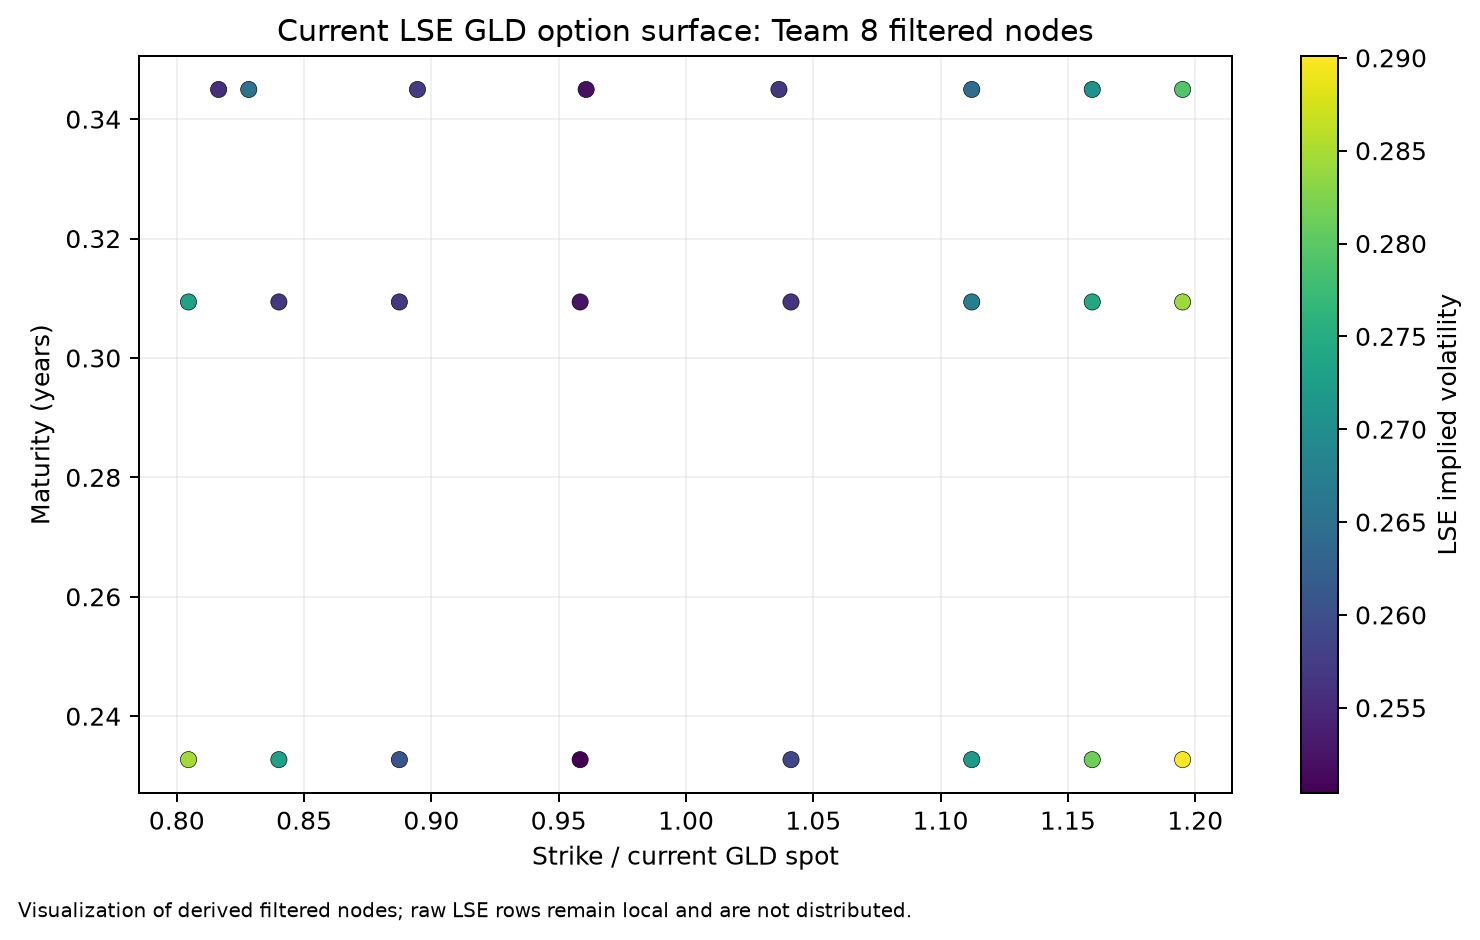
\includegraphics[width=0.88\textwidth]{img/lse/gld_option_surface_20260826.png}
\caption{Current GLD option nodes retained by the Team 8 filtering and
sampling logic. Color denotes LSE implied volatility. The surface is a
risk-neutral, IV-mapped object; it is neither a set of contemporaneous traded
prices nor a physical forecast of gold in USD/oz.}
\label{fig:gld-current-option-surface}
\end{figure}

On this 24-node sample, IV RMSE is 114.04 basis points for Black--Scholes,
86.28 for Heston, 56.55 for Bates--Poisson and 32.49 for Full
Bates--Hawkes. The richer specifications improve current in-sample fit, but
the mapped chronological source evidence still fails to establish
out-of-sample superiority over the previous-day implied-volatility surface.
Model complexity is therefore treated as a conditional representation of
option-price dynamics, not as evidence of a better physical gold forecast.
Moreover, the Full Bates--Hawkes branching ratio is 0.02, exactly the imposed
lower bound. The current cross-section therefore supports the model's combined
variance-and-jump flexibility more clearly than it identifies economically
strong self-excitation.


\part{Operations, Corporate Valuation, Validation and Conclusions}
% Unified chapter derived from the Team 4 source and maintained in this project.
\chapter{Production and Cost Forecasting}
\chapterstatus{Team 4 operating methodology refreshed with Barrick Q1--Q2 2026 actuals; price simulation and valuation demonstrator excluded.}
\sourceassetnote
\section{Introduction, Data and Definitions}
\subsection{Overview}
The accurate valuation of mining assets fundamentally relies on the precise estimation of future Cost of Sales (CoS). However, projecting these operational costs over a medium term horizon, specifically five years (or 20 quarters), presents significant statistical hurdles, most notably the management of variance within highly volatile commodities markets. When applied to isolated mining operations, standard econometric models frequently generate confidence intervals that are prohibitively wide for practical financial modeling, occasionally yielding illogical outputs such as negative costs or exponential growth trajectories. To mitigate these structural limitations, this paper introduces a hybrid Log-Space SARIMA framework.

Complementary to the cost side, the second pillar of operational profitability is gold production, the primary driver of the firm's revenue stream. Forecasting total output as a single time series is unsatisfactory: the heterogeneity of individual assets and the compounding of mine-specific shocks degrade the signal-to-noise ratio and inflate the resulting confidence intervals. To address this, we adopt a bottom-up physical decomposition into Ore Processed, Average Grade, and Recovery Rate, with the first two forecast through mine-level SARIMA models and the third simulated within historically observed operational bounds. Aggregate uncertainty is then evaluated using Goodman's exact variance-of-products approximation, which preserves the multiplicative structure of the production formula while avoiding the explosive variance of a naive product of confidence intervals.

Gold price risk is deliberately outside this chapter. The operating forecasts produced here are handed to the independent Team~8 price layer and to the unified DCF only after production and Cost of Sales have been constructed. This separation prevents the historical Team~4 price demonstrator from being confused with the gold scenarios and corporate valuation used in the unified experiment.
\subsubsection{Objective}
The objective is to build a five-year operating contract for Barrick's production and Cost of Sales. Due to the compounding volatility inherent in the mining sector, traditional top-down forecasting models frequently generate explosive variances and operationally impossible scenarios, such as negative costs or unbounded production. To resolve these structural limitations, this chapter proposes a bottom-up model. By decomposing operating performance into geological and metallurgical drivers, the approach aims to stabilise medium-term cost and production forecasts without producing a standalone price or valuation result.
\subsubsection{Data Sources}
All the non-market data used in this analysis were extracted from Barrick Gold Corporation's quarterly reports, available as PDF and/or Excel files on the company's investor website. The dataset concentrates on Barrick's largest gold mines; copper operations and smaller mines were excluded because they have a negligible impact on total production and revenue for the periods considered.

The mines included in the analysis are:
\begin{itemize}
  \item Bulyanhulu, Carlin, Cortez, Kibali, Loulo--Gounkoto, North Mara, Pueblo Viejo, Turquoise Ridge.
\end{itemize}
\subsubsection{Definitions of Financial and Process Metrics}
To ensure clarity in valuation, we adopt the standard definitions provided in the Barrick Annual Report 2024 \sourcecitation{barrick2024}.

\begin{definition}[Cost of Sales (Gold)]
Cost of sales applicable to gold production includes site operating costs, royalty expense, depreciation, and community relations costs. It excludes costs associated with sites in closure or care and maintenance. On a per-ounce basis, it is calculated as the cost of sales across operations divided by ounces sold (attributable basis).
\end{definition}


\begin{definition}[Ore tonnes processed]
Total physical volume of ore (gold-bearing rock) measured in tonnes, that has been extracted from the mine and fed into the processing plant.
\end{definition}

\begin{definition}[Average grade]
Concentration or richness of gold (measured in grams/tonne) within the ore that's being processed.
\end{definition}

\begin{definition}[Recovery rate]
Percentage of gold present in the ore successfully extracted. It measures the efficiency of the processing facilities.
\end{definition}

% ===============================
% Chapter : Methodology
% ===============================
\section{Cost of sales forecast methodology}
This chapter details the forecasting algorithm implemented in R. Before defining the final "Log-Space Delta-Anchor" model, we outline the investigative process and alternative approaches that were discarded, justifying the necessity of the chosen methodology. The data utilized for this study was gathered from Barrick Gold's quarterly reports for the selected mines previously mentioned in the introduction. Although historical data for certain mines extends back to 2016, a complete, continuous dataset devoid of missing values (NaNs) across all selected mines is only available from 2019 onward. Consequently, to ensure data integrity and consistency, only data from 2019 onwards has been used for the following analysis \sourcecitation{githubrepo}.

% Asset/code block omitted pending provenance acceptance.
\subsection{Evolution of the Modeling Strategy}
The development of the valuation model proceeded through three distinct iterations. The challenges encountered in the first two approaches directly informed the design of the final Global Master Chain framework.

\paragraph{Attempt 1 -- Fundamental Factor Modeling:}
Our initial approach aimed to construct a formal explanatory model based on the primary cost drivers identified in Barrick Gold's annual reports. Management explicitly lists \textbf{diesel prices, labor costs, and currency exchange rates} as the most significant factors impacting the Cost of Sales.

We attempted to model the Cost of Sales ($Y_t$) as a function of these exogenous variables:
\[ Y_t = \beta_0 + \beta_1(\text{Oil}_t) + \beta_2(\text{Labor}_t) + \beta_3(\text{FX}_t) + \varepsilon_t \]

However, this approach proved unfeasible for two reasons:
\begin{enumerate}
    \item \textbf{Data Granularity and Geography:} The mines are geographically dispersed across vastly different jurisdictions (e.g., Nevada, USA vs. Loulo--Gounkoto, Mali). Obtaining reliable, high-frequency historical data for local labor costs or specific energy tariffs in developing regions was extremely difficult.
    \item \textbf{Propagation of Uncertainty:} To forecast mining costs 5 years into the future, we would first need to forecast the drivers (e.g., the price of Brent Crude in 2029). The error associated with forecasting these macroeconomic indicators, combined with the model error, led to an explosion of uncertainty in the final output.
\end{enumerate}

\paragraph{Attempt 2 -- Idiosyncratic Univariate Forecasting:}
We subsequently moved to univariate time series models, applying standard forecasting algorithms directly to the data of each individual mine. We tested: ETS (Error, Trend, Seasonality) and Holt-Winters Exponential Smoothing.\\
Those failed due to sample size limitations. The reliable dataset covers the period from Q1 2019 to Q4 2025, providing approximately $N \approx 24$ data points per mine. Given the high operational volatility of individual sites (due to maintenance shutdowns, grade variations, or local disruptions), the signal-to-noise ratio was too low. The models frequently failed to converge or produced confidence intervals so wide that they encompassed negative costs, rendering them useless for valuation.

\paragraph{Final Approach -- The Global Master Chain Hypothesis:}

By overlaying the time series of all major mines (fig \sourceref{fig:ts overlay}) on a single plot, we observed synchronicity in the movements of Cost of Sales, particularly when analyzing relative changes rather than absolute dollar amounts. 

To statistically validate this visual intuition \sourcecitation{hair2018}, we analyzed the quarter-over-quarter cost shocks of the mines. The dataset was strictly filtered to include only data from 2019 onwards, ensuring a complete, balanced panel across all operations and cleanly capturing the recent era of heightened macroeconomic volatility.

First, a \textbf{Bartlett's Test} \sourcecitation{hair2018} was conducted on the correlation matrix of the mines' percentage cost changes. The test yielded a statistically significant result (\textbf{p-value = 0.0186}), allowing us to cleanly reject the null hypothesis that the mines' cost structures evolve independently.

Subsequently, a \textbf{Principal Component Analysis} (PCA) was performed to isolate and quantify this shared momentum \sourcecitation{hair2018}. The results provided robust quantitative support for the Global Master Chain Hypothesis: the first principal component (PC1) alone explains \textbf{41.22\% }of the total variance in cost shocks across the dataset. Furthermore, the first two principal components combined account for nearly 63\% (62.79\%) of all cost fluctuations, confirming a heavily macro-driven environment.

% Asset/code block omitted pending provenance acceptance.


In a real-world operational context, where individual physical assets are subject to severe local disruptions (e.g., distinct labor strikes, regional weather events, and varying ore grades), discovering that over 40\% of all cost volatility is dictated by a single, shared principal component is highly significant \sourcecitation{hair2018}.

This observation provided the empirical justification to adopt a Log-Space Beta scaling Anchor approach. This method consists of aggregating all mines to extract a stable global signal (the "Master Chain"), forecasts this stable signal, and then projects the trend back onto individual mines using a volatility scalar ($\beta$).

\subsection{Rationale for Logarithmic Transformation}
To implement this Global Master Chain, we apply a natural logarithm transformation to the Cost of Sales ($Y_t$). This step is critical for three econometric reasons specific to financial time series.

Financial time series often exhibit heteroscedasticity, where the volatility of the series increases as the level of the series rises. In mining, as input costs (energy, labor, steel) rise, the absolute dollar variance of the Cost of Sales tends to increase.

Standard linear models assume homoscedasticity (constant variance). By modeling $\ln(Y_t)$ rather than $Y_t$, we stabilize the variance, making the series more amenable to ARIMA modeling.

Inflation and cost escalation are inherently multiplicative processes. If costs grow by rate $r$, the process is defined as:
\[ Y_t = Y_{t-1} \cdot (1+r) \]
Linear models (like ARIMA) are additive. The logarithmic transformation converts this multiplicative relationship into a linear additive one:
\[ \ln(Y_t) = \ln(Y_{t-1}) + \ln(1+r) \]
This allows the linear SARIMA model to capture percentage growth rates rather than absolute dollar increments.

A standard Gaussian forecast on raw data ($Y_t$) carries a non-zero probability of predicting negative costs if the variance is sufficiently high or the trend is downward. By forecasting in log-space and exponentiating the result ($\hat{Y} = e^{\ln \hat{Y}}$), we mathematically guarantee that the forecasted Cost of Sales will strictly be non-negative ($\hat{Y} > 0$).
\subsubsection{The Global Master Chain (Log-Space)}
\begin{definition}[Log-Global Master Chain - Weighted]
Let $Y_{i,t}$ be the Cost of Sales for mine $i$ at time $t$. Let $Q_{i,t}$ represent the quantity extracted (e.g. ounces produced) for mine $i$ at time $t$. We first compute the weighted cross-sectional average $\bar{Y}_t$ by weighting each mine's cost by its relative production volume, and then apply the natural logarithm to obtain the master chain $M_t$:
\[
M_t = \ln(\bar{Y}_t) = \ln\left( \frac{\sum_{i=1}^{N} Q_{i,t} Y_{i,t}}{\sum_{i=1}^{N} Q_{i,t}} \right)
\]
\end{definition}
\subsection{SARIMA Model, Results and Validation}
Having established the Global Master Chain as a reliable proxy for the shared cost momentum across all mining operations, the next critical step is to forecast its future trajectory. To accomplish this, we utilize a Seasonal Autoregressive Integrated Moving Average (SARIMA) framework \sourcecitation{box1970} as our primary forecasting engine. 

This section details the complete modeling workflow applied to the log-transformed Master Chain. We begin by defining the mathematical structure and the strictly required statistical assumptions of the SARIMA algorithm. Following this theoretical foundation, we present the empirical results: the pre-modeling stationarity tests used to determine the necessary order of integration, the optimal parameter estimation selected via information criteria, and the rigorous residual diagnostics performed to ensure the model's structural validity. Finally, we provide an out-of-sample validation to empirically demonstrate the model's predictive accuracy before deploying it for the final five-year valuation projections.
\subsubsection{Mathematical Formulation of the SARIMA Model}
To forecast the Master Chain $M_t$, we employ a Seasonal Autoregressive Integrated Moving Average (SARIMA) framework. This class of models extends the standard ARIMA structure to explicitly capture both non-seasonal momentum and repeating seasonal cycles inherent in financial and operational time series.


A general $SARIMA(p,d,q)(P,D,Q)_s$ model is defined mathematically as.

\begin{definition}[SARIMA Formulation]
Let $y_t$ represent the observed value of the time series at time $t$. The generalized multiplicative SARIMA model is expressed as:
$$\phi(B)\Phi(B^s)(1-B)^d(1-B^s)^D y_t = c + \theta(B)\Theta(B^s)\varepsilon_t$$

Where the constituent variables and polynomials are defined as follows:
\begin{itemize}
\renewcommand{\labelitemi}{$-$}
    \item $y_t$: The modeled time series (in this context, the log-transformed Master Chain $M_t$).
    \item $B$: The backshift (lag) operator $B^k y_t = y_{t-k}$.
    \item $s$: The seasonal periodicity of the data (e.g., $s=4$ for quarterly financial reporting).
    \item $p, d, q$: The non-seasonal autoregressive order, degree of differencing, and moving average order, respectively.
    \item $P, D, Q$: The seasonal autoregressive order, degree of seasonal differencing, and seasonal moving average order, respectively.
    \item $\phi(B) = 1 - \phi_1 B - \phi_2 B^2 - \dots - \phi_p B^p$: The non-seasonal autoregressive polynomial, capturing the dependency of the current value on its immediate $p$ past values.
    \item $\Phi(B^s) = 1 - \Phi_1 B^s - \Phi_2 B^{2s} - \dots - \Phi_P B^{Ps}$: The seasonal autoregressive polynomial, capturing the dependency of the current value on its past values from $P$ previous seasonal cycles.
    \item $(1-B)^d$: The non-seasonal differencing operator, applied $d$ times to eliminate structural trends and achieve mean stationarity.
    \item $(1-B^s)^D$: The seasonal differencing operator, applied $D$ times to eliminate seasonal drift.
    \item $c$: The constant term or "drift", representing the underlying deterministic growth rate of the differenced series.
    \item $\theta(B) = 1 + \theta_1 B + \theta_2 B^2 + \dots + \theta_q B^q$: The non-seasonal moving average polynomial, modeling the influence of $q$ past forecast errors.
    \item $\Theta(B^s) = 1 + \Theta_1 B^s + \Theta_2 B^{2s} + \dots + \Theta_Q B^{Qs}$: The seasonal moving average polynomial, modeling the influence of past forecast errors from $Q$ previous seasonal cycles.
    \item $\varepsilon_t$: The white noise error term at time $t$, assuming independent and identically distributed innovations where $\varepsilon_t \sim WN(0, \sigma^2)$.
\end{itemize}
\end{definition}

This generalized framework allows the forecasting algorithm to systematically test and isolate both immediate, quarter-over-quarter cost momentum and delayed, year-over-year seasonal dependencies prior to model selection.
\subsubsection{Underlying Statistical Assumptions}
To ensure the mathematical validity of the SARIMA framework and the reliability of its subsequent forecasts, the model relies on several core statistical assumptions regarding the underlying data-generating process:

\begin{itemize}
    \item \textbf{Stationarity:} The time series, post-differencing ($d$ and $D$), must exhibit weak stationarity. This implies that its statistical properties specifically the mean, variance, and autocovariance are constant over time and independent of the specific time $t$ at which they are observed.
    \item \textbf{Linearity:} The model assumes that the current value of the series is a linear combination of its past values (autoregressive terms) and past error shocks (moving average terms).
    \item \textbf{Invertibility and Stability:} The roots of both the autoregressive polynomial $\phi(B)$ and the moving average polynomial $\theta(B)$ must lie strictly outside the unit circle. This guarantees that the model is mathematically stable (i.e., past shocks decay over time rather than explode) and uniquely identifiable.
    \item \textbf{White Noise Innovations:} The error terms (or innovations) $\varepsilon_t$ must be independently and identically distributed (i.i.d.) with a mean of zero and a constant variance $\sigma^2$ (homoscedasticity). Crucially, there must be no serial correlation between the residuals at any lag.
    \item \textbf{Normality of Residuals:} While accurate point forecasts can be generated without strict normality, the calculation of precise and symmetric confidence intervals explicitly assumes that the error terms $\varepsilon_t$ follow a Gaussian (normal) distribution.
\end{itemize}
\subsubsection{Model Selection and Validation}
Model selection was performed using an automated grid-search algorithm optimized for Information Criteria, allowing for both seasonal and non-seasonal terms. The algorithm identified an \textbf{ARIMA(3,1,0) with drift} as the optimal fit, minimizing both the Akaike Information Criterion \sourcecitation{akaike1974} (AIC = -94.64) and the Bayesian Information Criterion \sourcecitation{schwarz1978} (BIC = -86.87). Notably, the algorithm found no significant seasonal patterns to justify the inclusion of seasonal parameters.

The chosen model indicates that the series required first-order differencing ($d=1$) to stabilize the mean, followed by three autoregressive terms ($p=3$) to capture the temporal dependencies. 

The formal mathematical representation of the estimated ARIMA(3,1,0) model with drift, using the backshift operator $B$, is expressed as:

$$(1 + 0.9501B + 0.6128B^2 + 0.3003B^3)(1 - B)y_t = 0.0222 + \varepsilon_t$$

Where $y_t$ represents the log-transformed series, $0.0222$ is the estimated drift constant (representing the underlying linear trend of the differenced series), and $\varepsilon_t$ represents the white noise error term.
\subsubsection{Residual Diagnostics}
To ensure the structural validity of the selected model, the residuals were subjected to diagnostic testing. \\
 \textbf{Autocorrelation (Ljung-Box Test):} The Ljung-Box test \sourcecitation{ljung1978} returned a test statistic of $Q^* = 2.42$ with a p-value of \textbf{0.6585}. Failing to reject the null hypothesis confirms that the residuals do not exhibit significant autocorrelation and behave as independent white noise. \\
\textbf{Normality (Shapiro-Wilk Test):} The Shapiro-Wilk test \sourcecitation{shapiro1965} yielded a p-value of \textbf{0.6826}. This confirms that the residual distribution does not significantly deviate from a normal distribution, ensuring the reliability of the generated confidence intervals for future point forecasts.


To assess practical forecasting performance and guard against overfitting, the model was evaluated on a 12-period hold-out test set. The ARIMA(3,1,0) predictions were benchmarked against a Naive (Random Walk) forecasting model. 

The predictive accuracy was measured using Root Mean Squared Error (RMSE) and Mean Absolute Percentage Error (MAPE). 

% Asset/code block omitted pending provenance acceptance.


The ARIMA model demonstrated vastly superior predictive capabilities on unseen data. It achieved an RMSE three times lower than the benchmark model and maintained a remarkably low MAPE of \textbf{0.603\%}. This out-of-sample performance solidly justifies the use of the ARIMA(3,1,0) model for future predictions of this time series.

% Asset/code block omitted pending provenance acceptance.
\subsection{Volatility Scaling (\texorpdfstring{$\beta$}{beta})}
To project the global master trend onto individual mines, we cannot assume a 1:1 relationship. Some mines exhibit significantly higher operational risk than the global average due to specific geological or geopolitical factors. We estimate a specific volatility scalar, $\beta_i$ \sourcecitation{poon2003}.
\subsubsection{Regularization: Blume's Adjustment }
We define the raw volatility scalar $\beta_{raw,i}$ as the ratio of the standard deviation of the mine's historical log-returns to the standard deviation of the global master chain's historical log-returns.

Let $r_{i,t} = \Delta \ln(Y_{i,t})$ be the log-return of mine $i$, and $r_{global,t} = \Delta M_t$ be the global log-return.
\[
\beta_{raw,i} = \frac{\sigma(r_{i,t})}{\sigma(r_{global,t})}
\]

It is crucial to note that this metric differs from a standard financial Beta (CAPM), which is defined as $\rho_{i,m} \cdot \frac{\sigma_i}{\sigma_m}$. We deliberately exclude the correlation coefficient ($\rho_{i,m}$) from our calculation. In cost forecasting, a low correlation between a specific mine and the global index often indicates high \textit{idiosyncratic} risk (e.g., local strikes, wall collapses) rather than stability. A regression-based Beta would dampen the projected volatility for uncorrelated assets, leading to dangerously narrow confidence intervals. By utilizing the simple ratio of standard deviations, we ensure that the forecast envelope fully reflects the mine's total historical instability, regardless of its correlation with the global cycle.


Given the limited sample size ($N \approx 30$ quarters per mine), the raw $\beta_{raw,i}$ estimates are subject to significant sampling noise. Extreme values (e.g., $\beta > 3.0$) are often artifacts of single outlier events rather than persistent structural characteristics.

To mitigate this, we apply Blume's Adjustment \sourcecitation{blume1975}, a shrinkage technique used in finance to adjust beta estimates towards the market mean of 1.0. This assumes that over the long run, extreme volatility characteristics tend to revert to the mean, which is a reasonable assumption to make given that the cost of sales is highly dependent on oil and fuel prices that exhibit strong volatility clustering.

The adjusted beta $\beta_{adj,i}$ is calculated as a weighted average:
\[
\beta_{adj,i} = w \cdot \beta_{raw,i} + (1 - w) \cdot 1.0
\]
We utilize the standard weighting of $w = 0.67$ (assigning 2/3 weight to the observed data and 1/3 to the prior assumption of market neutrality).

\[
\beta_{final,i} = 0.67 \cdot \frac{\sigma(r_{i,t})}{\sigma(r_{global,t})} + 0.33
\]

This regularization prevents the model from projecting explosive volatility for mines with short-term historical shocks, while still respecting their relative risk profile.
\subsubsection{Log-Space Projection}
Let $A_{i} = \ln(Y_{i, T})$ be the "Anchor", the logarithm of the last observed actual value for mine $i$. The forecast for $h$ steps ahead is calculated by accumulating the forecasted global deltas ($\Delta \hat{M}$), scaled by the mine's beta:

\[
\ln(\hat{Y}_{i, T+h}) = A_{i} + \sum_{k=1}^{h} (\Delta \hat{M}_{T+k} \times \beta_i)
\]

The 95\% Confidence Interval (CI) radius from the global ARIMA model ($R_{global}$) is also scaled by $\beta_i$. Finally, we exponentiate the results to return to real dollar values:

\begin{align*}
    \text{Forecast Value: } & \hat{Y}_{i, T+h} = \exp\left( \ln(\hat{Y}_{i, T+h}) \right) \\
    \text{Upper CI: } & \hat{U}_{i, T+h} = \exp\left( \ln(\hat{Y}_{i, T+h}) + (\beta_i \cdot R_{global, T+h}) \right) \\
    \text{Lower CI: } & \hat{L}_{i, T+h} = \exp\left( \ln(\hat{Y}_{i, T+h}) - (\beta_i \cdot R_{global, T+h}) \right)
\end{align*}

This geometric reconstruction ensures that the forecast can never be negative and that the growth rates are consistent with the historical volatility of the specific asset.
\subsection{Forecast Results}

The final outputs of the developed forecasting framework are visualized below. First, the algorithm computes the projected trajectory of the Global Master Chain (Figure \sourceref{fig:masterchain_forecast}), representing the underlying macroeconomic cost baseline. Subsequently, this global signal is scaled according to each asset's specific volatility profile and anchored to its latest reported costs, yielding the individual projections for the individual mines (Figure \sourceref{fig:shifted_forecast}).

% Asset/code block omitted pending provenance acceptance.


% Asset/code block omitted pending provenance acceptance.


The Log-Space Delta-Anchor method successfully mitigated the "exploding variance" problem often seen in long-term linear forecasting. By anchoring to the last actual value ($Y_{i,T}$) and operating in log-space, the projections maintain a consistent growth path. The Year-1 forecasts for 2026 align closely with the guidance ranges provided in the Barrick 2025 Annual Report \sourcecitation{barrick2025}.


% ===============================
% Chapter 3:  Production Forecast
% ===============================
\section{Production Forecast Methodology}

In order to derive a robust approximation of Barrick Gold's future revenue stream, we must first accurately forecast the primary driver of that revenue: gold production. 

Attempting to forecast total gold production as a single time series yields unsatisfactory results due to the inherent differences between the individual mining operators and their compounding volatility. A component-based approach is therefore preferred. In this context, we break down production into its fundamental physical factors: \textbf{Ore Processed}, \textbf{Average Grade}, and \textbf{Recovery Rate}. 

Furthermore, to align our output with standard financial reporting, we apply a unit conversion from metric tonnes to Troy Ounces (oz) by multiplying the result by $\frac{1}{31.11}$. Finally, we incorporate a historical realization factor of $0.91$. This factor represents the mean ratio across all mines between theoretical production and true realized output. It effectively accounts for the "delayed" nature of processing circuits, such as stockpiling, leaching pad dynamics, and autoclave residence times, where processes initiated in one quarter may not yield sale-able metal until subsequent quarters \sourcecitation{githubrepo}.
\subsection{The Production Formula}
The deterministic equation governing quarterly production is defined as follows:

\begin{equation}
    \text{Production (oz)} = \text{Ore Processed} \cdot \text{Average Grade} \cdot \text{Recovery Rate} \cdot 0.91 \cdot \frac{1}{31.11}  
\end{equation}

The expected future production will be computed forecasting the variables within this formula. To do so, a programmatic pipeline was developed in Python to process, analyze, and simulate data for each major asset. The methodology is broken down into four distinct computational phases.

\paragraph{Phase 1 -- Data Preprocessing and Structuring:}
Mining data frequently suffers from reporting gaps, particularly in the early stages of an asset's lifecycle or post-acquisition. The algorithm first cleans the dataset by identifying and removing leading null values (NaNs) to establish a continuous, reliable time series. For example, in the analysis of the Carlin complex, the algorithm isolates a clean, unbroken dataset comprising 28 historical quarters spanning from Q1 2019 to Q4 2025. While for North Mara, the historical quarters are 25, starting from Q4 2019, since that was the time the mine could be analyzed individually from the reports.

\paragraph{Phase 2 -- Operational Correlation and Bottleneck Analysis:}
Before forecasting, the script conducts a correlation analysis to uncover hidden operational dynamics between the production components. Two critical metallurgical phenomena were identified:

\begin{itemize}
    \item \textbf{Dilution and Bulk Mining Strategy:} The algorithm detected a negative correlation ($ r\approx -0.45$) between \textit{Ore Processed} and \textit{Average Grade}. Operationally, this indicates a "bulk mining" strategy. To increase total tonnage processed, the mine must extract lower-quality, marginal parts of the orebody or blend high-grade ore with lower-grade stockpiles. This process, known as dilution, artificially lowers the average grade as volume increases.
    
    \item \textbf{Plant Bottlenecks and Residence Time:} The analysis revealed a weak-to-moderate negative correlation ($r \approx -0.17$) between \textit{Ore Processed} and the \textit{Recovery Rate}. This highlights a fundamental plant bottleneck: processing facilities are engineered for an optimal flow rate (throughput). Pushing excess ore through the circuit reduces the "residence time" that a gold-bearing particle spends in chemical or physical extraction. Consequently, chemical reactions do not fully complete, leading to more valuable metal being lost to tailings (waste) and driving down the overall recovery rate.
\end{itemize}


\paragraph{Phase 3 -- Time Series Modeling (SARIMA):}
Given the seasonal nature of mining (e.g., wet seasons affecting haulage, scheduled winter maintenance, etc), traditional linear regressions are insufficient. The algorithm applies Seasonal AutoRegressive Integrated Moving Average (SARIMA) models to both \textit{Ore Processed} and \textit{Average Grade}. 

\begin{enumerate}
\item Ore Processed: the model has a parameter specification of \textit{SARIMA} $(1,0,1)$x$(1,0,0,4)$. 
    \begin{itemize}
        \item The autoregressive dependence on the immediately preceding quarter (non-seasonal AR=1) captures the "inertia" of the plant.
        \item The moving average (MA=1) captures the "shock" recovery from the previous quarter.
        \item The seasonal autoregressive dependence on the same quarter from the previous year (seasonal AR=1, $s=4$).
    \end{itemize}

\item Average Grade: the model has a parameter specification of \textit{SARIMA} $(1,0,0)$x$(0,0,0,4)$. 
    \begin{itemize}
        \item The autoregressive dependence on the immediately preceding quarter (non-seasonal AR=1).
        \item The moving average (MA=1) "shock" recovery.
    \end{itemize}
\end{enumerate}

The choice of these models is based on the intrinsic characteristics of these variables. First, mill throughput is a mechanical variable, requiring a stationary framework ($d=0, D=0$) that oscillates around a stable, optimized mean rather than trending toward zero or infinity. We then know that when a short-term mechanical failure causes a drop in throughput, operators push the mill to clear the accumulated run-of-mine (ROM) stockpiles. The autoregressive and moving average components ($p=1, q=1$) are set to capture the plant's operational inertia and its "catch-up" mechanics.  Finally, the seasonal autoregressive term ($P=1$ with an annual frequency of $m=4$) accounts for the cyclicality of mining physics, recognizing that quarterly throughput naturally fluctuates due to recurring weather constraints, such as winter freezing in Nevada or tropical wet seasons in Mali and the Dominican Republic. 

On the other hand, for average grade, we first recognized that the underlying rock chemistry is immune to surface weather cycles and then doesn't have seasonal parameters ($P,D,Q = 0$). The grade does not inherently fluctuate because it is winter or the wet season. Then, mining operations progress sequentially through large, continuous physical blocks of the earth. If the excavators are in a high-grade zone this quarter, they will likely still be in that rich zone next quarter. We capture this by setting the autoregressive component to $p=1$, and this is also why $q=0$, there is no "rebound" in rock chemistry. Subsequently, while a mine's overall grade naturally depletes over a 30-year lifespan, over our 5 year forecast horizon, mine planning teams actively manage the Run-of-Mine stockpile. They deliberately blend high-grade and low-grade ores to feed a consistent, stable average into the processing plant ($d=0$).


\paragraph{Phase 4 -- Stochastic Simulation of Recovery Rates:}
Unlike tonnage or grade, which are largely determined by mine plans and geological block models, metallurgical recovery is bounded by strict physical and chemical limitations. Because it cannot trend infinitely upward or downward, applying a SARIMA model to the Recovery Rate is mathematically inappropriate. 

Instead, the algorithm treats the future recovery rate as a stochastic variable, simulating it using a Uniform Distribution $U(\min, \max)$ bounded by the mine's historical operational extremes, with a $\pm$1\% adjustment, a 50\% floor and 100\% ceiling. For instance, Carlin's recovery is randomly sampled between $0.71$ and $0.85$, for each forecasted period, perfectly encapsulating the inherent variance of the processing plant without imposing a false trend.
\subsection{Synthesis and Forecast Outputs}
In the final step, the algorithm executes the Production Formula across the forecasted arrays. By combining the deterministic SARIMA outputs with the stochastic uniform distribution and scaling by the realization factor, the script generates an expected annual production trajectory complete with 80\% Confidence Intervals (CI).
\subsubsection{Confidence Intervals}
The computation of confidence intervals is problematic if we consider the product of three separate components for the production forecast. We want a 80\% CI for the final product, for the production.
The confidence interval of the product can not be just the product of the confidence intervals of the components, because in doing that we would create a "worst-case scenario", where the intervals are too wide and operationally useless.

To make an example, taking the 80\% bounds for the components, the probability of them hitting their extreme 10\% lower tail would be $0.1\cdot0.1\cdot0.1 = 0.001$. By multiplying the three confidence intervals together we are no longer calculating the 80\% CI, but the 99.9\%.

Trying to create a more realistic analysis, we assume that the components tend to balance each other out through the law of large number. For example, if the grade is slightly lower than expected this quarter, the mill operators might push the throughput slightly higher than expected to make up for it.

Therefore, to create an 80\% CI for total production, we use a statistical method called \textbf{Goodman's Exact Variance of Products}.
\subsubsection{Goodman's Formula}
Published in 1960 by Leo A. Goodman \sourcecitation{goodman1960}, this formula calculates how uncertainties compound geometrically when variables are multiplied together. The original formula for three variables, considering $X$(Ore processed), $Y$(Average grade) and $Z$(Recovery rate), is as follow:

\begin{equation}
    Var(XYZ) = \mu_X^2 \mu_Y^2 \sigma_Z^2 + \mu_X^2 \mu_Z^2 \sigma_Y^2 + \mu_Y^2 \mu_Z^2 \sigma_X^2 + \mu_X^2 \sigma_Y^2 \sigma_Z^2 + \mu_Y^2 \sigma_X^2 \sigma_Z^2 + \mu_Z^2 \sigma_X^2 \sigma_Y^2 + \sigma_X^2 \sigma_Y^2 \sigma_Z^2
\end{equation}

Then, instead of dealing with raw variances and to avoid long computations, we convert the uncertainty of each variable into a Coefficient of Variation (or Relative Error), denoted as $R$. 

Relative error is the standard deviation divided by the expected mean.

\begin{equation}
    R_X=\frac{\sigma_X}{\mu_X}
\end{equation}

In this way, Goodman's formula can be rearrange as follow:

\begin{equation}
    R_{prod}^2 = (1 + R_X^2)(1 + R_Y^2)(1 + R_Z^2) - 1
\end{equation}

\begin{equation}
    \sigma_{prod}=R_{prod}\cdot\mathbb{E}_{prod}  \footnote{$\mathbb{E}_{prod}$ is the expected production computed with the forecast of the components, using the production base formula \sourceref{eq:production}}
\end{equation}

\begin{equation}
    CI_{lower} = \max(0, \mathbb{E}_{prod} - Z_{score} \cdot \sigma_{prod})
\end{equation}

\begin{equation}
CI_{upper} = \mathbb{E}_{prod} + Z_{score} \cdot \sigma_{prod}
\end{equation}

This Goodman equation assumes independent variables, and we saw from subsection 3.2.2 that they are not. However, because we don't have a lot of historical data ($\approx$ 28 quarters each mine), computing covariances could create severe noise. Otherwise, a negative correlation naturally stabilizes the final product, producing a wider margin of error and generating a conservative bound.

\textit{Note:} Recovery rate is generated using a uniform distribution. Since it does not have CI, its variance is computed taking the historical maximum has the upper bound. In the equations $Z_{score} = 1.282$, corresponding to the $80\%$ confidence level used throughout this chapter.

\begin{equation}
    \sigma_{recovery}=\frac{Max_{historical}-\mu_{forecast}}{Z_{score}}
\end{equation}

This component-based methodology ensures that the final aggregate forecast is grounded in metallurgical reality, preventing the explosive, unbounded variance typical of standard long-term commodity forecasting.
\subsection{Single mine plots \& total results}
In this section we first plot the historical gold production for every mine, by quarters.

% Asset/code block omitted pending provenance acceptance.


We then plot the four graphs of the Carlin mine as the baseline output example.

% Asset/code block omitted pending provenance acceptance.


The production forecast algorithm forecasts the following profile (in thousands of ounces) over the 5-year horizon:

% Asset/code block omitted pending provenance acceptance.


In this final part we plot the total company production, with historical and forecasted data, by quarters. As we can see, the last year production was lower then the historical mean and had a bump down in 2nd and 3rd quarter of 2025. This was due to the temporary closure of Loulo--Gounkoto mine for geopolitical reasons. 

% Asset/code block omitted pending provenance acceptance.


% Asset/code block omitted pending provenance acceptance.
\subsubsection{Uncertainties and Unknown Events}
Events like the closure of Loulo--Gounkoto may happen for specific mines and should be considered in the forecast of the production; nevertheless we thought about different reasons of why it would be an over complication of the model. 

Because Barrick is a massive, globally diversified company, these localized risks rarely happen all at once. These operational shocks are isolated to a specific mine or region, rather than being systemic. Therefore, we believe that the probability of simultaneous failure is statistically negligible. In the production forecast, we relied on the fact that the shocks would be absorbed, both geographically and over time.
\subsection{Current operating evidence and the forecast handoff}

The operational decomposition developed by Team~4 is retained, but its
empirical inputs are refreshed with Barrick's Q1 and Q2 2026 mine-statistics
tables. The current evidence is deliberately limited to physical production,
ore processed, processed grade, recovery and Cost of Sales. The standalone
article's NSS curve, option inversion, GBM paths and illustrative stochastic
EBITDA valuation are not inputs to this thesis valuation.

Figures~\ref{fig:team4-production-qoq} and
\ref{fig:team4-cost-qoq} compare the two available 2026 quarters for the
eight-mine analytical perimeter. The selected mines produced 622 attributable
koz in Q1 and 711 koz in Q2; the difference from Barrick's company totals of
719 and 796 koz is expected because the company totals include other
operations. Company-wide Cost of Sales was USD~1,922/oz in Q1 and
USD~1,993/oz in Q2.

\begin{figure}[htbp]
    \centering
    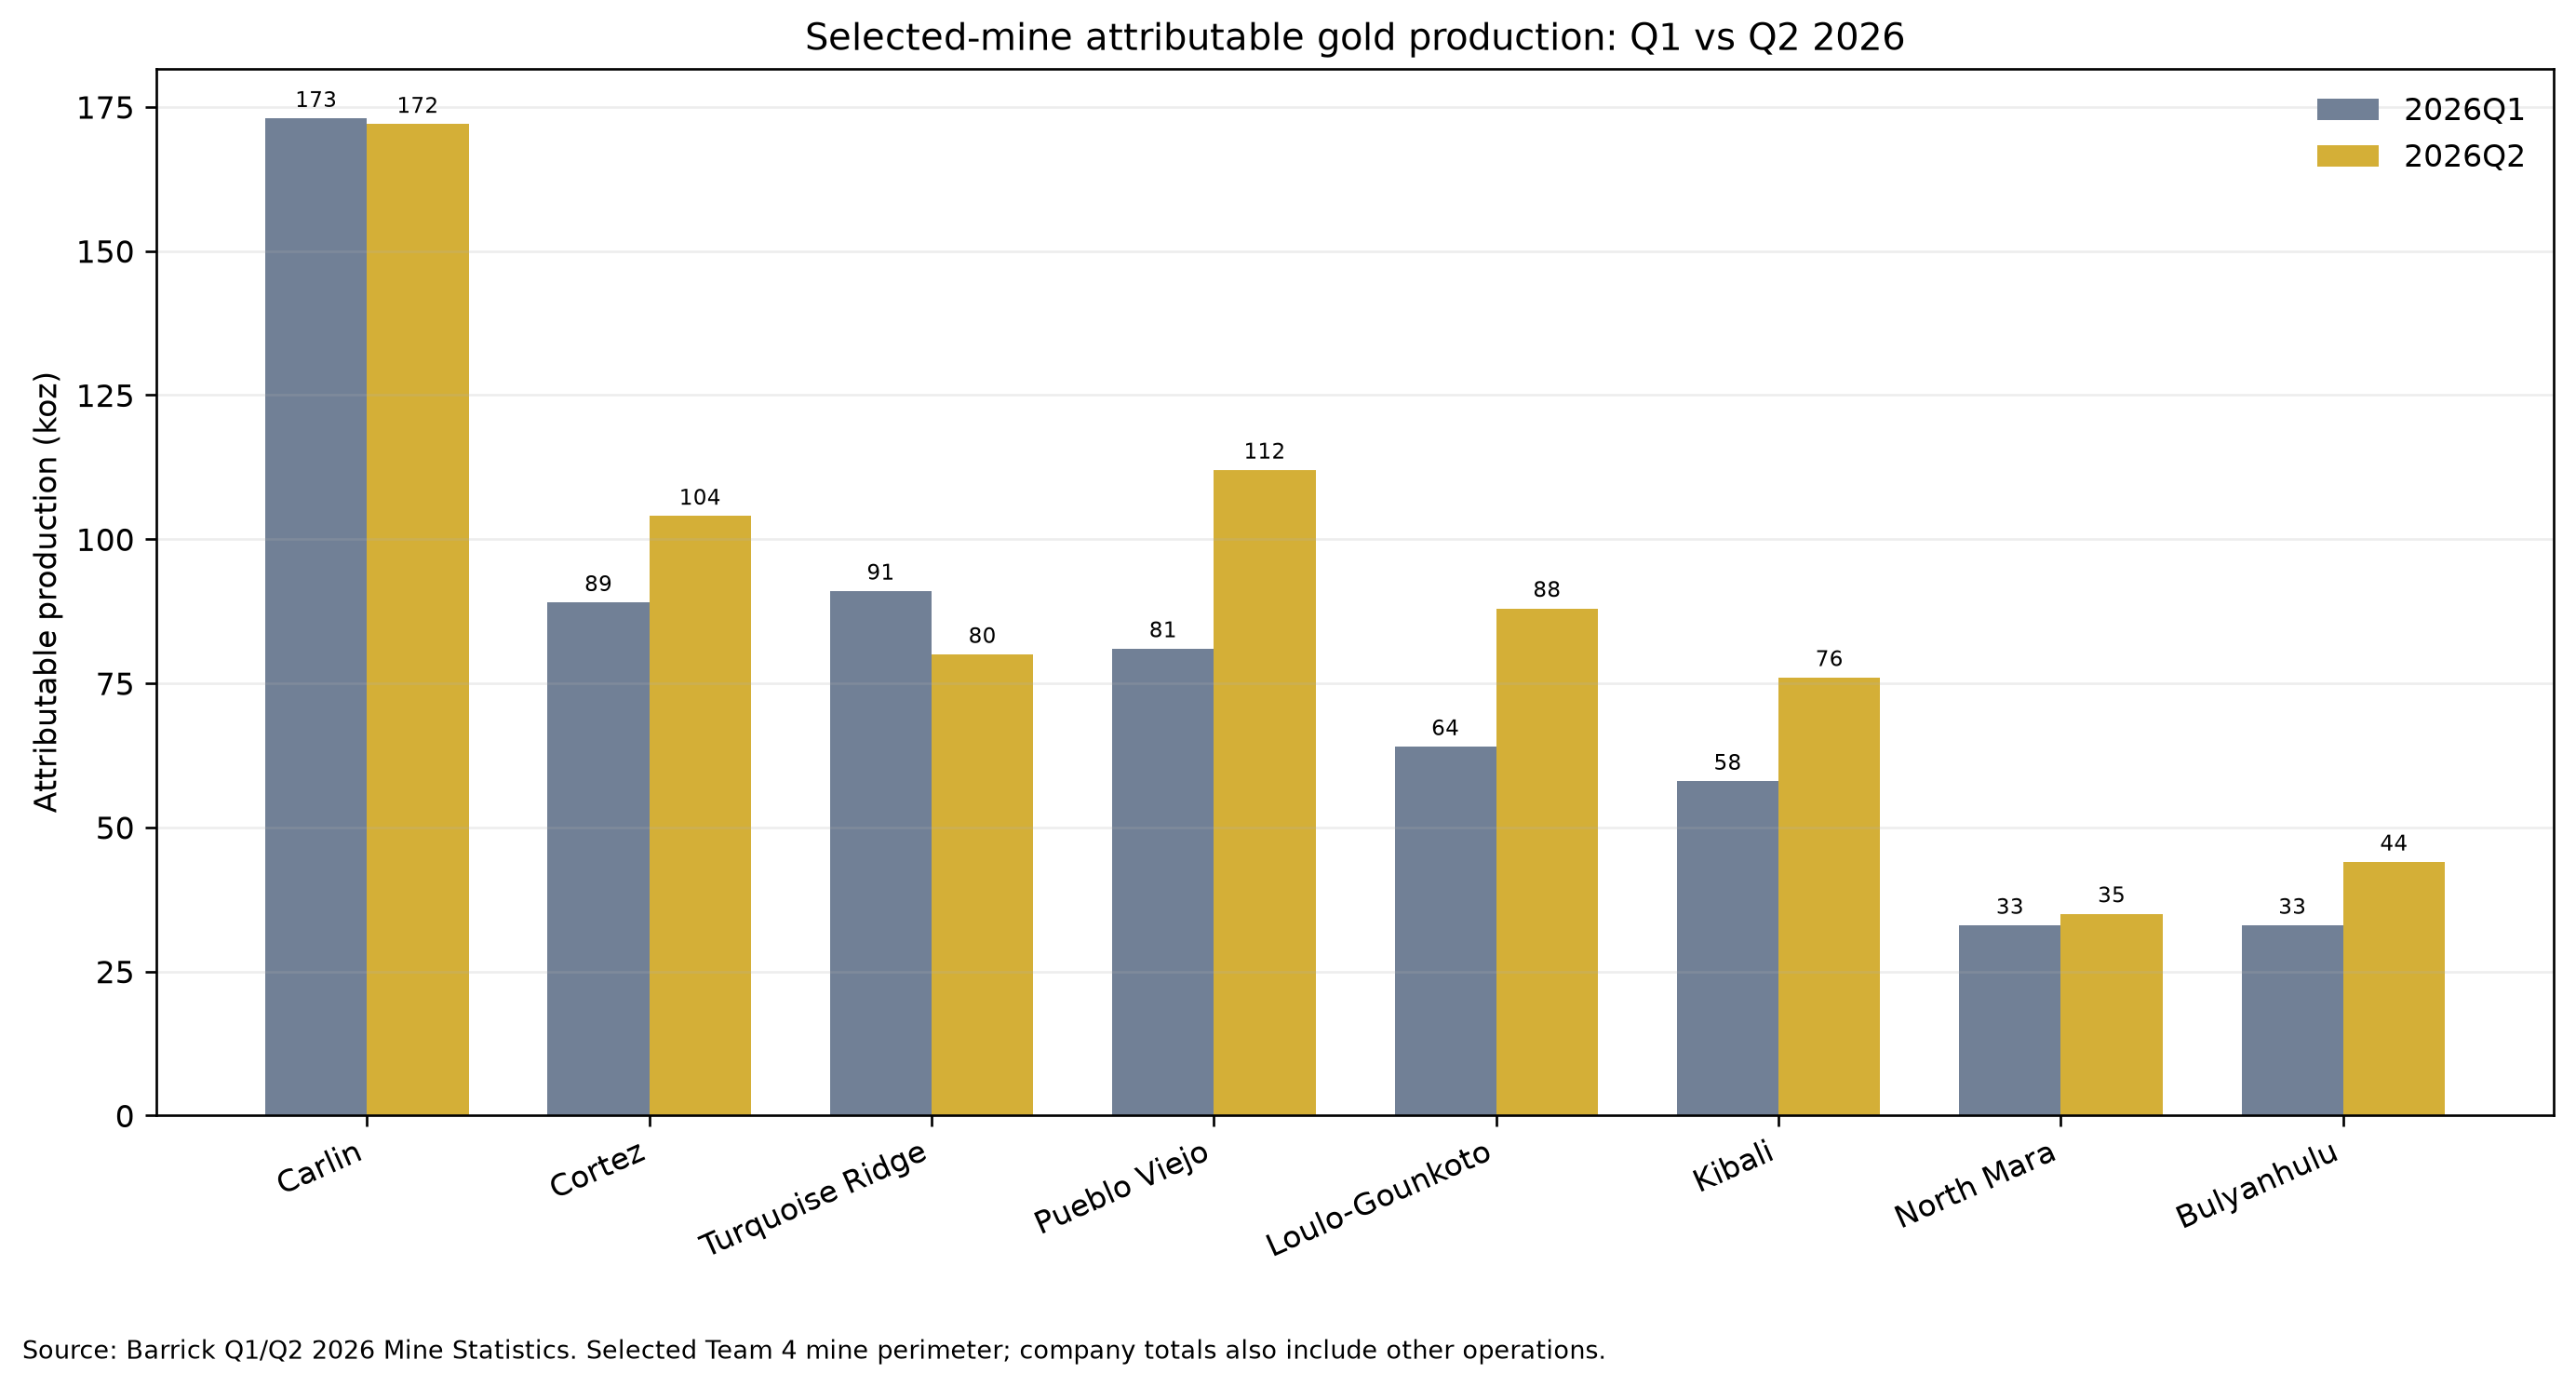
\includegraphics[width=\textwidth]{img/team4_current/team4_mine_production_qoq.png}
    \caption{Attributable gold production for the eight mines retained from
    the Team~4 study, refreshed from Barrick's Q1 and Q2 2026 Mine Statistics.
    These bars are current observations, not simulated production paths.}
    \label{fig:team4-production-qoq}
\end{figure}

\begin{figure}[htbp]
    \centering
    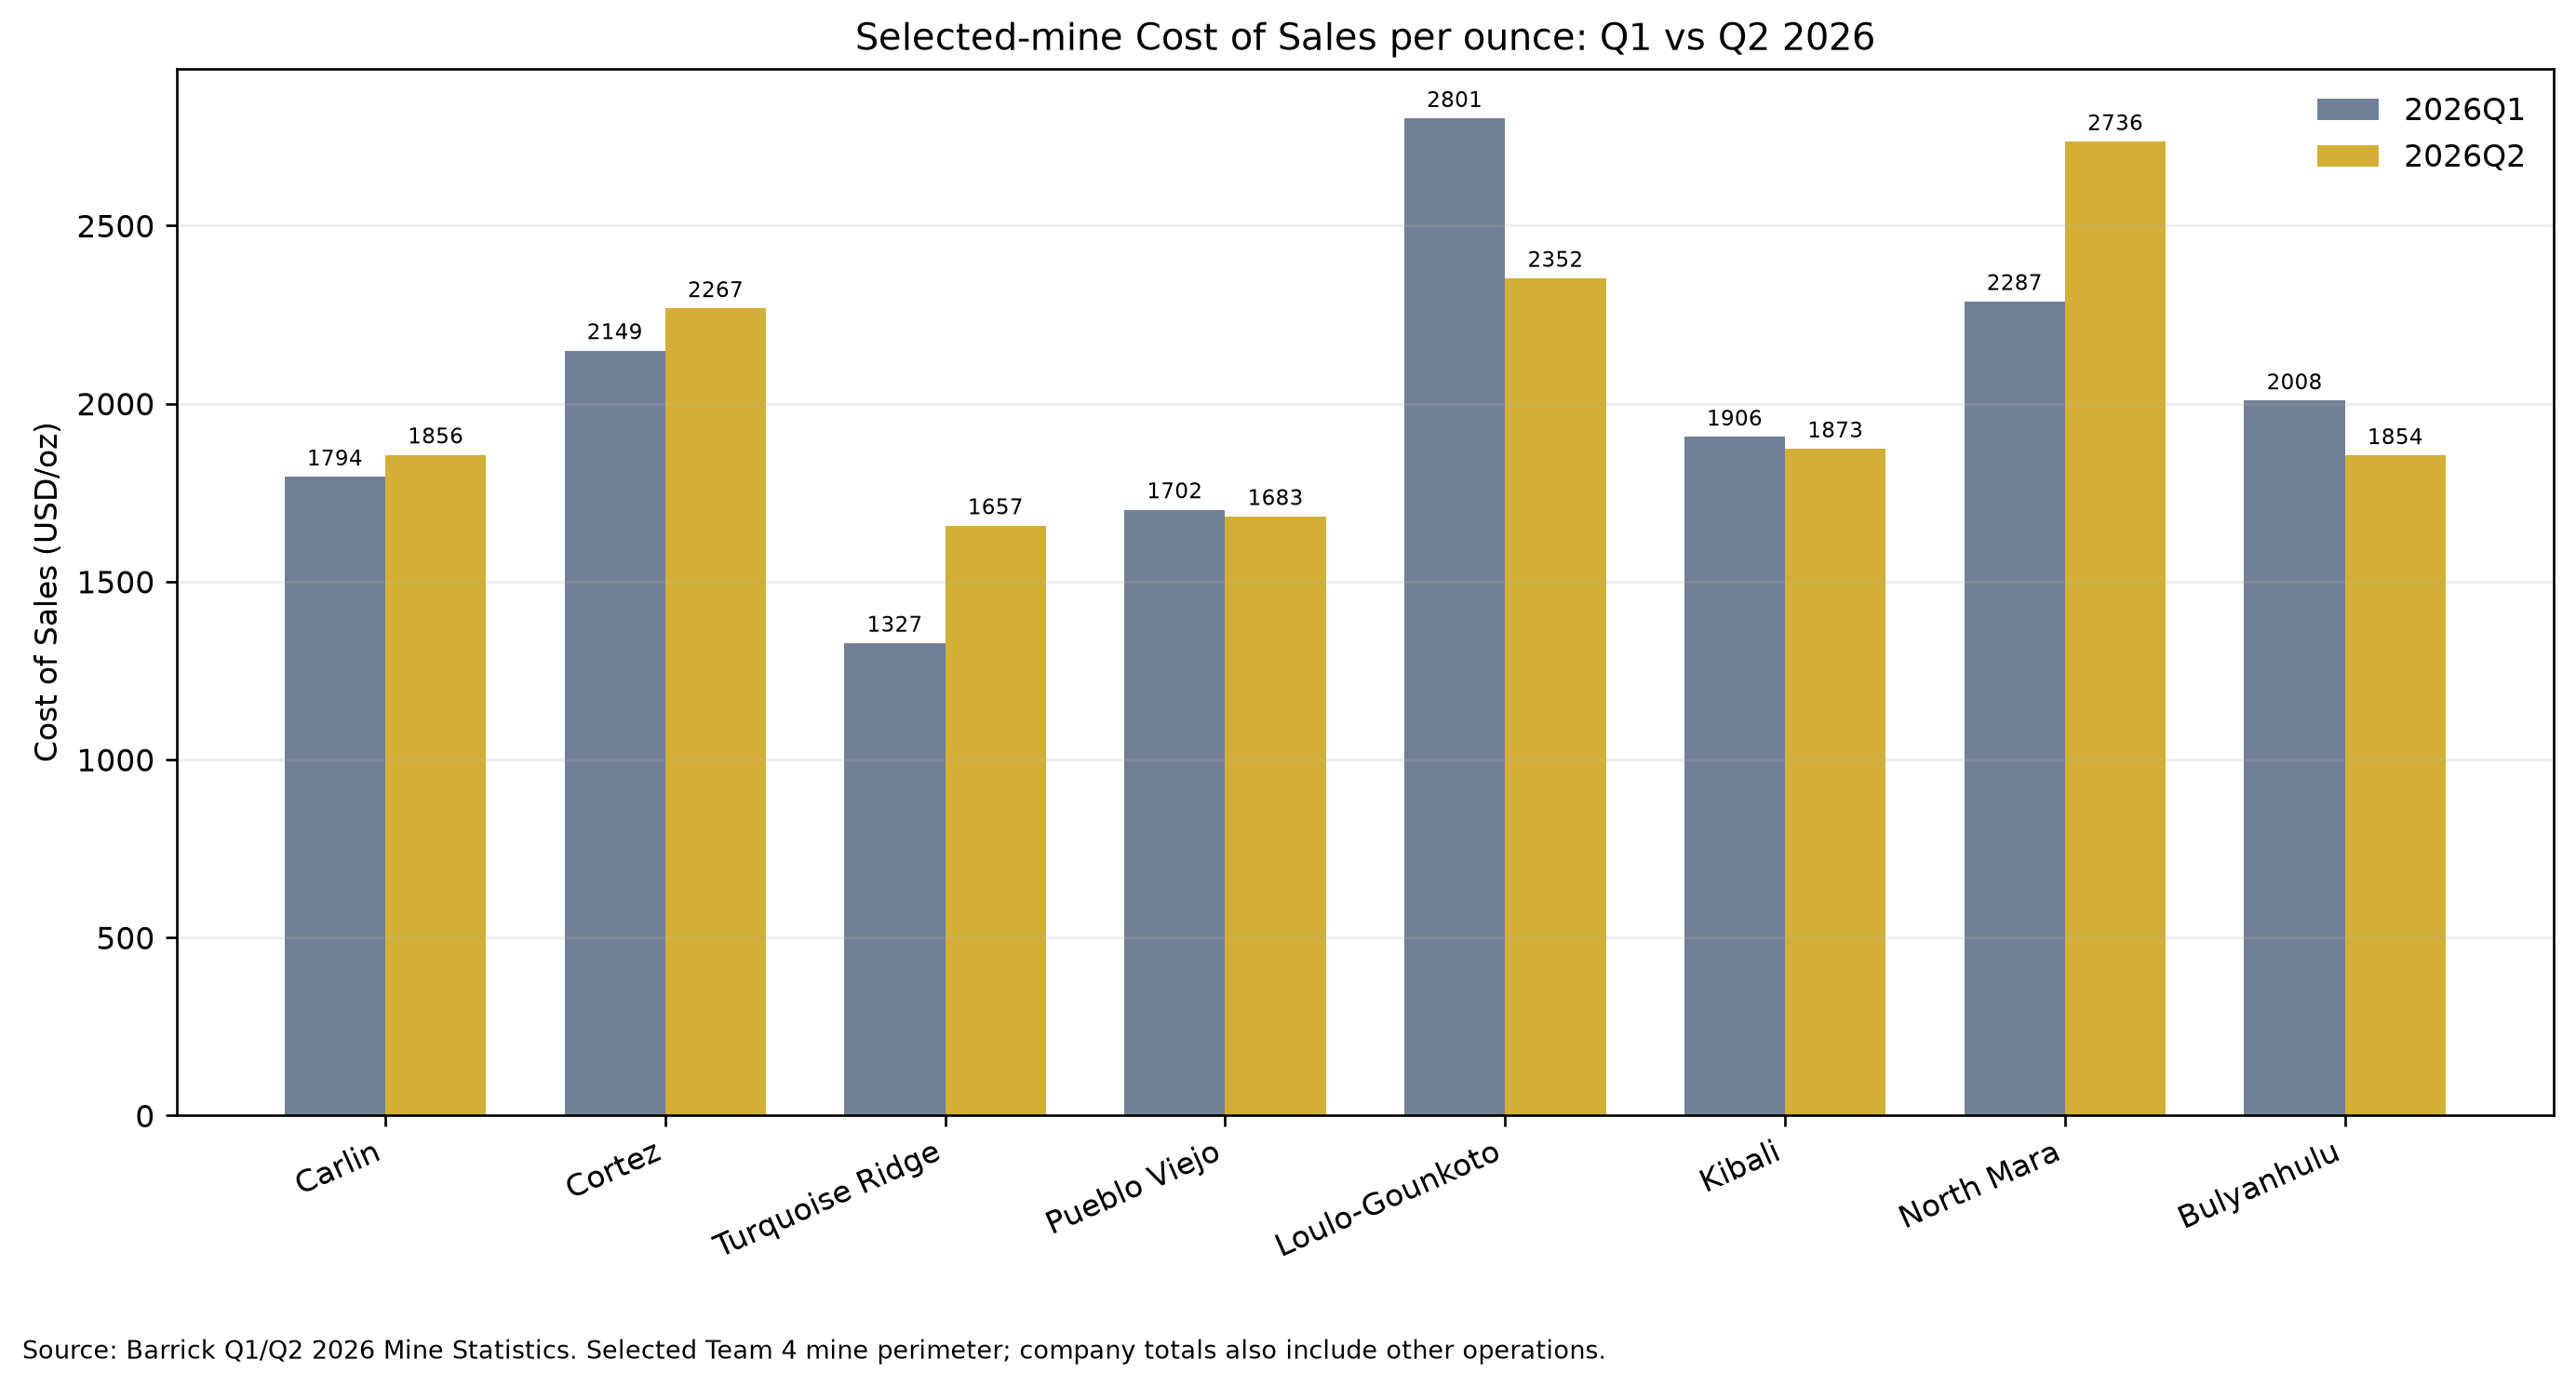
\includegraphics[width=\textwidth]{img/team4_current/team4_mine_cost_qoq.png}
    \caption{Cost of Sales per ounce for the same mine perimeter. The figure
    preserves the Team~4 mine-level comparison while replacing article images
    with a branch-local rendering of current public data.}
    \label{fig:team4-cost-qoq}
\end{figure}

The physical drivers behind production are shown separately in
Figure~\ref{fig:team4-process-components}. This matters because tonnes,
grade and recovery can move in opposite directions: a production change
cannot be interpreted as a price effect, and none of these panels contains a
gold-price input.

\begin{figure}[p]
    \centering
    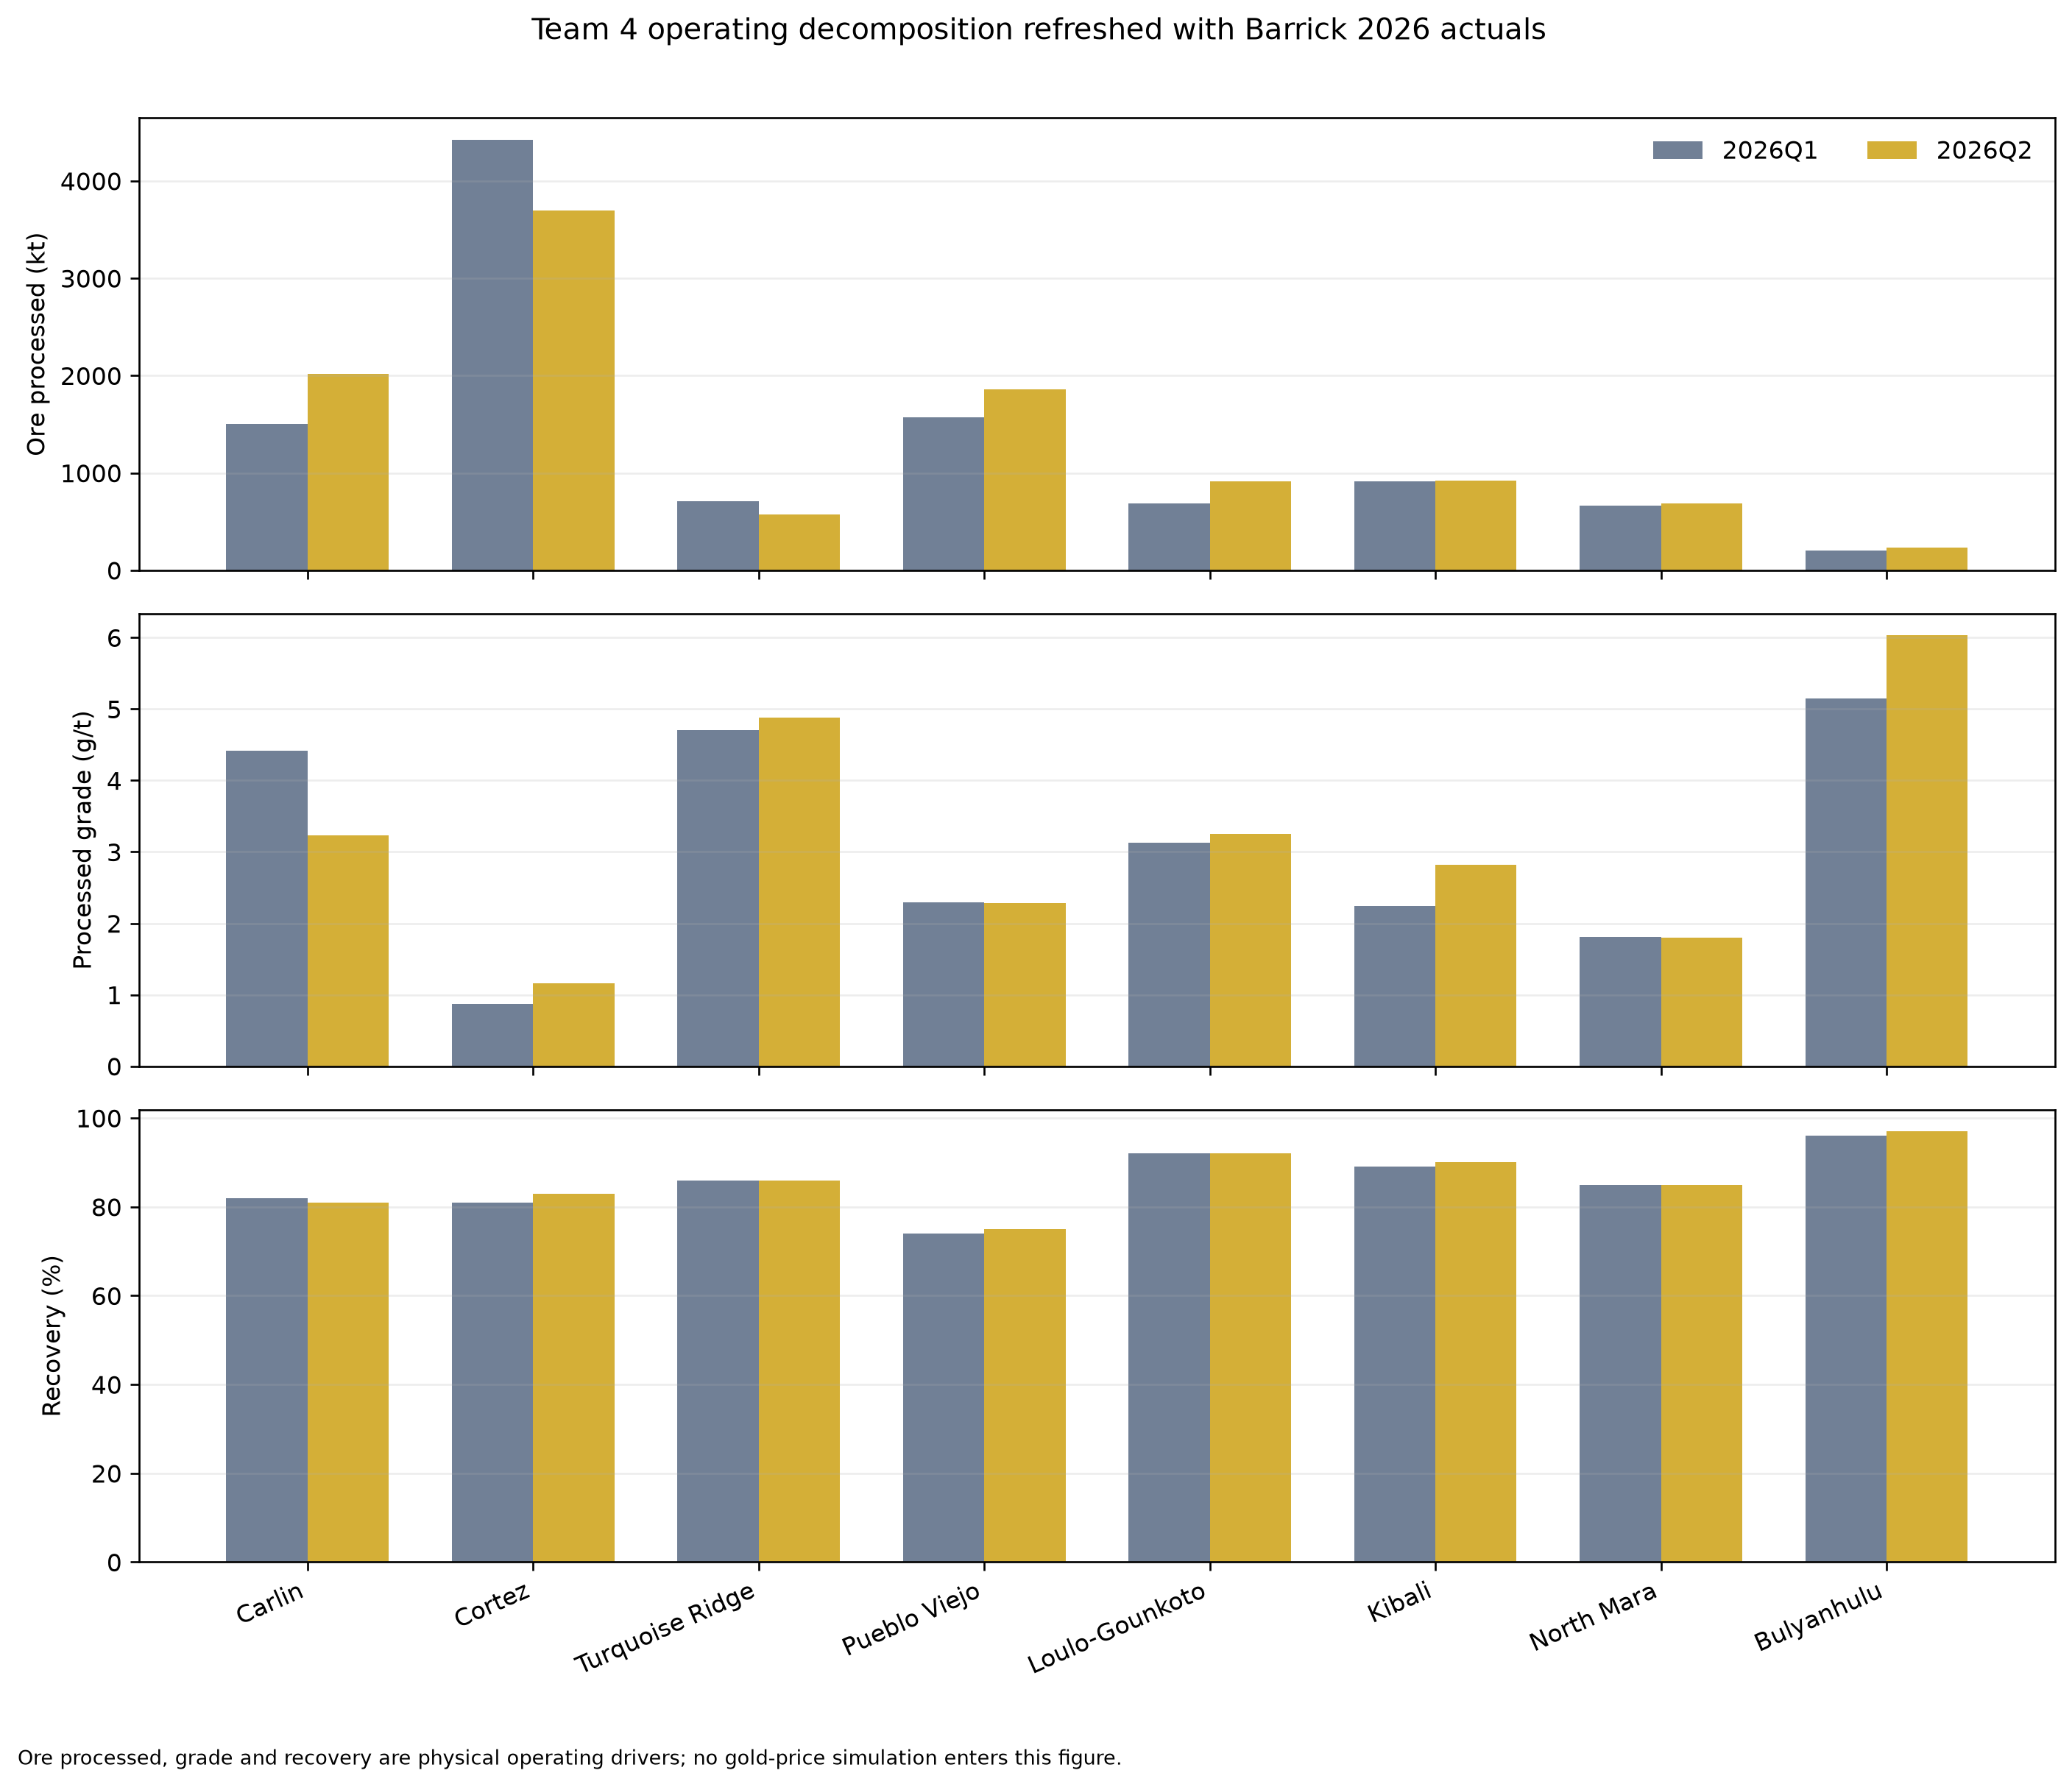
\includegraphics[width=\textwidth]{img/team4_current/team4_process_components_qoq.png}
    \caption{Ore processed, processed grade and recovery in Q1 and Q2 2026.
    Values are transcribed from Barrick's published mine-statistics tables and
    generated by code in this branch.}
    \label{fig:team4-process-components}
\end{figure}

The DCF horizon needs a complete 20-quarter operating vector. The clean
handoff is therefore mixed but explicit: 2026Q1--Q2 are Barrick actuals,
whereas 2026Q3--2030 retain the Team~4 forecasts. Figure~
\ref{fig:team4-operating-contract} marks the boundary in both code and
graphics. This avoids describing a forecast as observed evidence and prevents
the Team~4 price demonstrator from entering the valuation by association.

\begin{figure}[htbp]
    \centering
    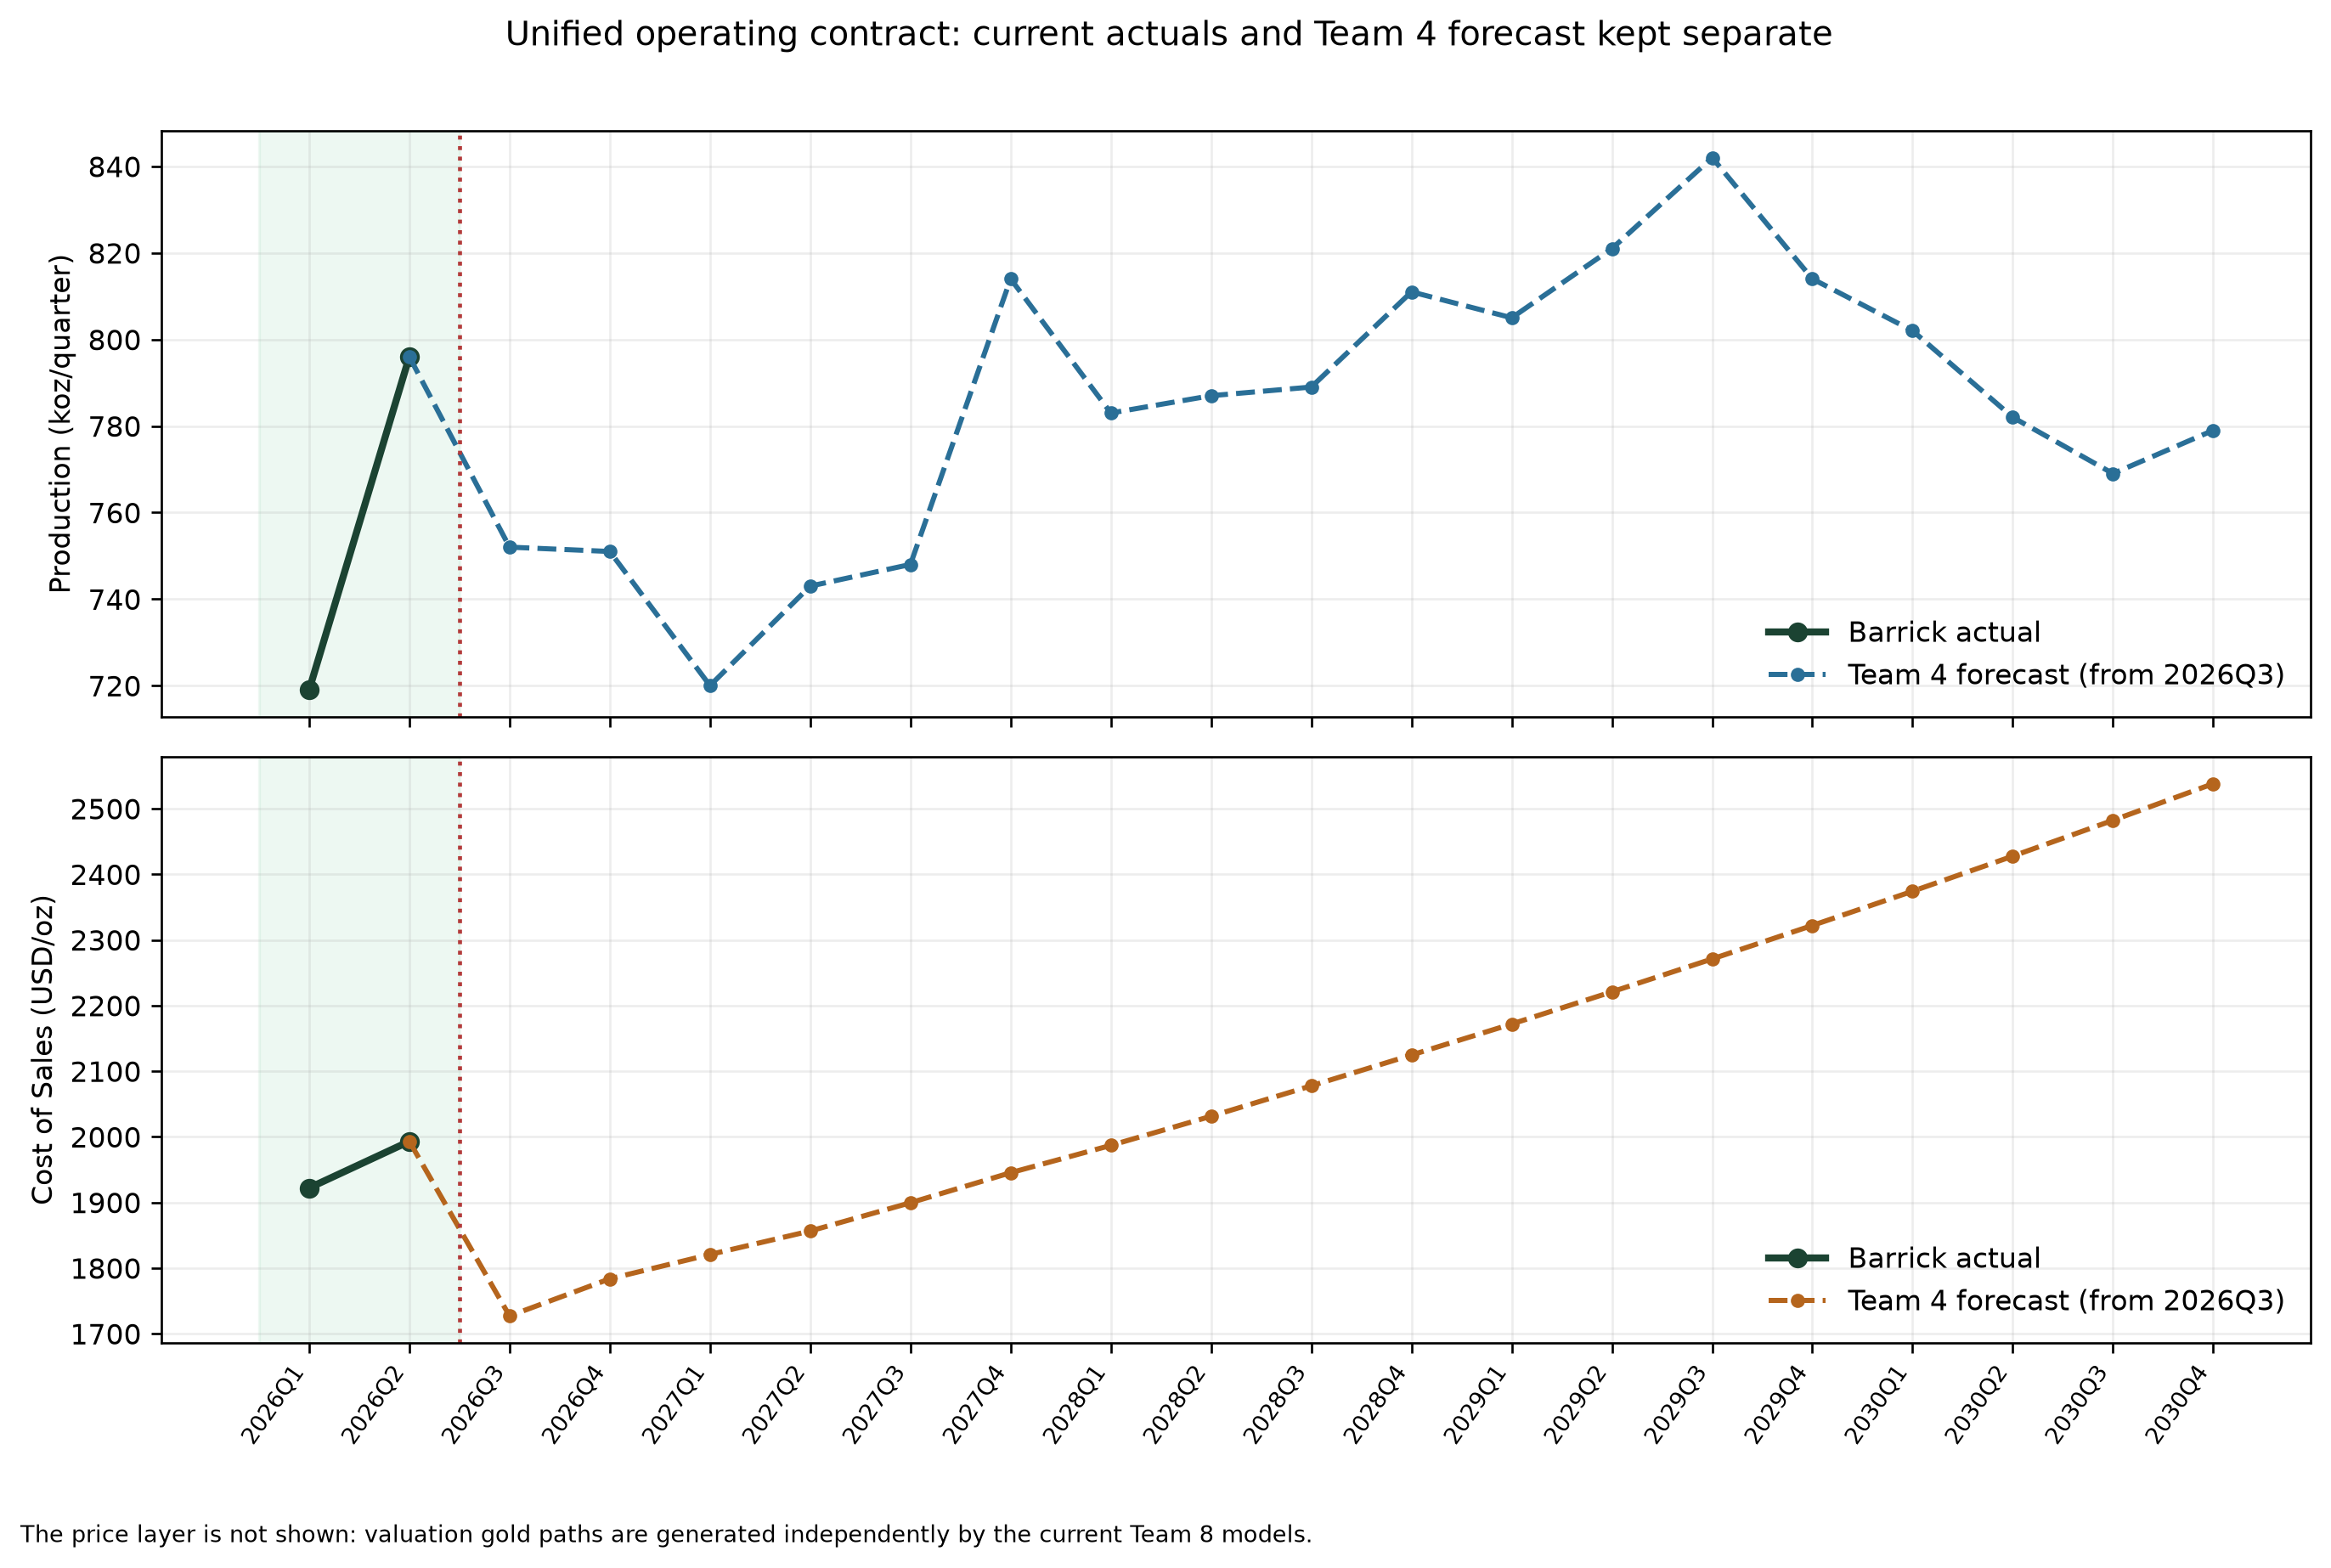
\includegraphics[width=\textwidth]{img/team4_current/team4_operating_contract.png}
    \caption{Operating contract consumed by the unified valuation. Green
    observations are current Barrick actuals; dashed values from 2026Q3 onward
    are Team~4 forecasts. The price layer is absent by design and is supplied
    independently by the current Team~8 models in Chapter~9.}
    \label{fig:team4-operating-contract}
\end{figure}

The remaining operating limitation is economic rather than procedural. The
forecast does not yet model reserves, mine closures, grade-dependent
management actions or endogenous production responses to adverse gold-price
states. Those items remain within the validation boundary and the genuinely
open research agenda; constructing a richer price model is no longer a
Team~4 ``next step'', because that work is already performed in Chapters~8--9.


\section{Handoff to the independent price and valuation layers}

The operating layer ends with production and Cost of Sales. For a quarterly
gold scenario \(P_t\), the pre-reconciliation component margin passed to the
DCF is
\[
    M_t=(P_t-\mathrm{CoS}_t)\,\mathrm{Production}_t .
\]
This identity is retained from Team~4, but \(P_t\) is not generated by the
Team~4 article. Chapter~9 supplies the four current Team~8 price engines and
Chapter~12 performs the corporate valuation. The old NSS--IV--GBM--EBITDA
sequence was useful as a standalone demonstration of an integrated stochastic
DCF; including it here would create a second, incompatible price process and
would blur the provenance of the valuation.

The separation is enforced in three places. First, the branch configuration
uses Barrick's Q2 2026 average realized gold price only as a documented common
level anchor, not as a spot quote or forecast. Second, quarterly risk-neutral
rates come from the current Team~8 LSE Treasury input rather than the Team~4
NSS fit. Third, all simulated paths come from Black--Scholes, Heston,
Bates--Poisson or Bates--Hawkes under one common conditional bridge. Thus
Team~4 contributes operational mechanics and forecasts only; it contributes
no simulated gold price and no standalone valuation output.

\subsection{Limitations carried forward}

The 2026Q1--Q2 refresh removes the earlier lack of current operating evidence,
but it does not turn the later Team~4 values into management guidance. From
2026Q3 onward they remain research forecasts. Mine depletion, reserve lives,
closures, recovery interventions, cost inflation by jurisdiction and
price-dependent management actions are not endogenous. These are live model
limitations. By contrast, richer stochastic volatility and jump models are
not future work for this chapter: they have already been implemented and
tested in Chapters~8--9, then propagated through the unified experiment in
Chapter~12.

\chapter{A Three-Stage DCF Framework for Mining Valuation}
\chapterstatus{Expanded reconstruction from Team 5. The original article
provides accounting reclassification, FCFF/FCFE, WACC, three-stage transition
and a reproducible synthetic Monte Carlo illustration. This chapter retains
those supported methods, corrects the terminal-value cash-flow definition and
adapts the framework to a finite-resource miner. Synthetic values are never
reported as Barrick estimates.}

\section{Valuation object: firm value before equity value}

% Sources: Team 5 ch-2, ch-4 and 3df; CONTENT-LEDGER BG-U-11.
Discounted cash flow is not one formula but a consistency system linking a
cash-flow definition, the claim being valued and the corresponding discount
rate. Team 5 distinguishes two coherent routes. The equity route discounts
free cash flow to equity at the cost of equity,
\begin{equation}
EqV_0=\sum_{y=1}^{H}\frac{FCFE_y}{\prod_{s=1}^{y}(1+k_{e,s})}
      +\frac{TV_H^{Eq}}{\prod_{s=1}^{H}(1+k_{e,s})},
\end{equation}
whereas the firm route discounts FCFF at WACC and values all operating claims
before financing:
\begin{equation}
EV_0=\sum_{y=1}^{H}\frac{FCFF_y}{\prod_{s=1}^{y}(1+w_s)}
     +\frac{TV_H^{Firm}}{\prod_{s=1}^{H}(1+w_s)}.
\end{equation}
The unified experiment adopts the firm route because the Team 4 operating
layer produces pre-financing drivers. For scenario \(m\), enterprise value is
converted to equity and then to a per-share quantity only through an explicit
bridge:
\begin{align}
EqV^{(m)}
  &=EV^{(m)}-\text{net debt}-\text{minority and other claims}
    +\text{admitted non-operating assets},\\
V_{ps}^{(m)}&=\frac{EqV^{(m)}}{N_{dil}}.
\end{align}
The signs, scale, currency, security and date of every bridge item are part of
the valuation result. A direct FCFE calculation cannot be used to hide an
unreconciled capital structure.

\begin{table}[H]
\centering
\small
\begin{tabularx}{\textwidth}{@{}p{2.7cm}p{3.0cm}p{2.8cm}X@{}}
\toprule
Route & Cash flow & Discount rate & Output and principal consistency test \\
\midrule
Firm valuation & FCFF before debt service & WACC & Enterprise value; operating
cash flows must exclude financing and be reconciled to invested capital. \\
Equity valuation & FCFE after net borrowing & Cost of equity & Equity value;
leverage policy and net borrowing must be modelled explicitly. \\
\bottomrule
\end{tabularx}
\caption{The two DCF routes recovered from Team 5. Mixing FCFF with the cost of
equity, or FCFE with WACC, changes the claim being valued and is inadmissible.}
\label{tab:dcf-route-consistency}
\end{table}

\section{Reclassifying financial statements for valuation}

% Sources: Team 5 ch-3; GAP-DCF-01 and GAP-VAL-05.
Standard statements mix operating, non-operating and financing items. Team 5's
reclassification is therefore a prerequisite, not an optional presentation
step. The operating side of invested capital can be expressed as
\begin{equation}
IC_y=OWC_y+PP\&E_y+\text{other net operating assets}_y,
\end{equation}
after excluding excess cash, marketable securities and other admitted
non-operating assets. The financing side must reconcile to debt and equity
claims. Return on invested capital is then
\begin{equation}
ROIC_y=\frac{NOPAT_y}{IC_{y-1}},
\end{equation}
so the comparison \(ROIC_y-w_y\) measures value creation from operating
capital rather than accounting earnings alone.

Operating working capital excludes cash and debt items that belong to the
financing bridge. In a mining application, inventories, receivables, payables,
royalties, reclamation provisions, streaming obligations and tax balances
must be assigned consistently. PP\&E and mine development also require care:
depreciation is an accounting allocation, sustaining capex is a cash outflow,
and closure liabilities are neither interchangeable nor automatically
contained in AISC.

NOPAT isolates after-tax operating profit from financing:
\begin{equation}
NOPAT_y=EBIT_y-\text{operating cash taxes}_y
       \approx EBIT_y(1-\tau_y),
\end{equation}
where the approximation is valid only when the tax rate and deferred-tax
adjustments are appropriate to the operating perimeter. Interest expense,
interest tax shields and income on excluded assets do not belong in NOPAT.

\begin{table}[H]
\centering
\small
\renewcommand{\arraystretch}{1.10}
\begin{tabularx}{\textwidth}{@{}p{3.0cm}p{4.2cm}X@{}}
\toprule
Block & Valuation treatment & Mining-specific control \\
\midrule
Revenue and operating cost & Build EBIT before financing. & Reconcile ounces,
realised price, ownership, royalties and whether cost metrics include D\&A or
sustaining investment. \\
Working capital & Include operating receivables, inventories and payables. &
Do not treat cash, debt or financing balances as operating working capital. \\
PP\&E and development & Link depreciation, capex and asset base. & Separate
sustaining, growth and closure expenditure; avoid counting AISC and capex
twice. \\
Taxes & Estimate operating cash taxes. & Separate current/deferred taxes,
jurisdictional effects and financing tax shields. \\
Non-operating and financing items & Exclude from FCFF and admit through the
EV-to-equity bridge. & Reconcile cash, debt, minorities, streams, other claims
and diluted shares to one filing date. \\
\bottomrule
\end{tabularx}
\caption{Financial-statement reclassification required before the operating
simulation can be called an FCFF model.}
\label{tab:dcf-reclassification}
\end{table}

\section{Operating forecasts and the FCFF contract}

% Sources: Team 5 ch-4 and ch-5; Team 4 interface.
Team 5 starts from sales, costs, margins, depreciation and working capital.
For a miner, the generic sales-growth shortcut is replaced by the more
informative component identity
\begin{equation}
Revenue_y^{(m)}=Q_y^{(m)}P_y^{realised,(m)}+\text{other operating revenue}_y^{(m)},
\end{equation}
where production \(Q\), realised price \(P^{realised}\), ownership and hedging
must share units and period conventions. Cost ratios can still be used as
checks, but a constant COGS-to-sales assumption is weak when grades, strip
ratios, energy, labour and mine mix change independently of price.

The admitted cash-flow identity is
\begin{align}
\text{Reinvestment}_y^{(m)}
  &=CapEx_y^{(m)}-D\&A_y^{(m)}+\Delta NWC_y^{(m)},\\
FCFF_y^{(m)}
  &=NOPAT_y^{(m)}-\text{Reinvestment}_y^{(m)}.
\end{align}
Every component uses the same sign convention: a rise in operating working
capital consumes cash, depreciation is non-cash, and capex consumes cash. CoS,
cash cost, AISC, royalties and D\&A cannot be combined until a data dictionary
proves what each aggregate already contains.

Team 5 also links growth to investment productivity. If expected operating
growth is \(g_y\) and the return on new invested capital is represented by
\(ROIC_y\), then
\begin{equation}
\text{reinvestment rate}_y=\frac{g_y}{ROIC_y},
\qquad
FCFF_y=NOPAT_y\left(1-\frac{g_y}{ROIC_y}\right).
\end{equation}
This identity prevents a model from assuming growth without funding it. It is
a consistency check rather than a licence to estimate Barrick's growth or
ROIC from the gold or equity-price series.

\section{Discount rate: currency, risk and capital structure}

% Sources: Team 5 ch-6; GAP-VAL-03/08.
Under the firm route, the pathwise or dated WACC is
\begin{equation}
w_y=\frac{E_y}{D_y+E_y}k_{e,y}
  +\frac{D_y}{D_y+E_y}k_{d,y}(1-\tau_y).
\end{equation}
A conventional CAPM estimate writes
\begin{equation}
k_{e,y}=R_{f,y}+\beta_y ERP_y+CRP_y,
\end{equation}
where any country-risk premium must match the geographic exposure and must not
be counted again in cash-flow haircuts. Beta requires an explicit convention:
a raw historical regression, smoothed beta or bottom-up unlevered/relevered
peer beta can produce different answers. The cost of debt may come from a
traded yield, recent borrowing spread or synthetic rating, but it must reflect
the same currency and horizon as the cash flows.

The risk-free input is conceptually a default-free zero-coupon rate matched to
the cash-flow maturity. A single long bond is only a proxy. Capital weights
should use market values and a target structure coherent with the forecast,
not book weights selected for convenience. If option-implied risk is already
embedded in the scenario distribution, the measure policy must also explain
why discounting does not charge for the same risk twice.

\section{Three stages and gradual convergence}

% Sources: Team 5 3df and montecarlo_int.
The three-stage model separates a high-growth or explicit phase, a transition
phase and a stable or closing phase. Its central contribution is gradual joint
convergence. Growth, operating margin, reinvestment, ROIC, leverage and risk
cannot jump independently at the terminal date. For a driver \(x\) that moves
from \(x_{hg}\) at the end of the first phase to \(x_s\) at year \(H\), a
transparent linear transition is
\begin{equation}
x_y=x_{hg}-\frac{y-H_1}{H-H_1}(x_{hg}-x_s),
\qquad H_1<y\leq H.
\end{equation}
The same device may be applied to several drivers, but their joint path must
remain economically coherent: lower growth normally implies lower incremental
reinvestment; mature margins and ROIC must be supportable; beta, leverage and
WACC should converge toward a defensible long-run state.

When perpetual continuation is economically admissible, Team 5's terminal
block is corrected to use post-horizon free cash flow rather than EBIT alone:
\begin{equation}
TV_H^{(m)}=
\frac{NOPAT_{H+1}^{(m)}
\left(1-g_s^{(m)}/ROIC_s^{(m)}\right)}
{w_H^{(m)}-g_s^{(m)}},
\qquad w_H^{(m)}>g_s^{(m)}.
\end{equation}
The denominator condition is necessary but not sufficient. Stable growth must
remain compatible with the valuation currency, long-run economy, reinvestment
capacity and return on new capital.

\section{Executable assumption register for the current experiment}
\label{sec:executable-valuation-assumptions}

The equations above describe the reusable method; this section discloses the
numbers actually passed to the current unified run. They are read from
\path{config/provisional_valuation_20260827_team4_separated.json}, not inferred
from the plotted valuation output. All four price branches use the same values.
They are deliberately classified as methodological assumptions because no
filing-level WACC, invested-capital reconstruction or mine-closure calibration
currently supports them as Barrick point estimates.

\begin{table}[H]
\centering
\caption{Editable non-gold parameters used by the current executable valuation.}
\label{tab:current-editable-valuation-parameters}
\scriptsize
\setlength{\tabcolsep}{3pt}
\renewcommand{\arraystretch}{1.10}
\begin{tabularx}{\textwidth}{@{}p{3.15cm}p{1.35cm}X X@{}}
\toprule
Configuration field & Current & Where it enters & Interpretation and effect \\
\midrule
\texttt{model.tax\_rate} & 25.0\% & Converts component margin to an
after-tax proxy. & Higher tax lowers explicit and terminal FCFF. \\
\texttt{model.high\_growth} & 8.5\% & First point of the five-year linear
growth schedule. & Raises early reinvestment through \(g/ROIC\); it does not
directly grow the operating margin paths. \\
\texttt{model.stable\_growth} & 2.5\% & Last schedule point and terminal
growth \(g_s\). & Changes terminal reinvestment and the \(w-g\) denominator. \\
\texttt{model.roic\_high} & 14.5\% & First point of the ROIC schedule. & At
fixed growth, higher ROIC reduces required reinvestment. \\
\texttt{model.roic\_stable} & 10.5\% & Last ROIC and terminal return. & Sets
terminal reinvestment \(g_s/ROIC_s=23.81\%\). \\
\texttt{model.wacc\_0} & 9.1\% & Initial state of the WACC process. & Affects
the conditional path from which years 1--5 are drawn. \\
\texttt{model.wacc\_long\_run} & 8.3\% & Mean-reversion level. & Pulls later
discount rates toward 8.3\%. \\
\texttt{model.wacc\_reversion} & 0.45 & Annual reversion speed. & Controls how
quickly the initial 9.1\% approaches the long-run level. \\
\texttt{model.wacc\_volatility} & 0.9\% & Diffusion scale of annual WACC. &
Widens the discount-rate and terminal-value distributions. \\
\texttt{model.terminal\_}\newline\texttt{spread\_floor} & 1.0\% & Lower-bound distance above
stable growth. & Enforces \(w_y\geq g_s+1\%=3.5\%\), with a separate 25\% cap. \\
\texttt{equity\_bridge.*} & zeros & EV-to-equity bridge. & Debt, cash,
minorities, other claims and non-operating assets are unresolved placeholders. \\
\texttt{diluted\_shares\_mn} & 1,675.51 & Equity value per share. & Unreconciled
proxy; changing it rescales every per-share distribution. \\
\bottomrule
\end{tabularx}
\end{table}

The five annual schedule points are generated by \texttt{numpy.linspace}.
Growth therefore moves through 8.5\%, 7.0\%, 5.5\%, 4.0\% and 2.5\%; ROIC moves
through 14.5\%, 13.5\%, 12.5\%, 11.5\% and 10.5\%. The corresponding
reinvestment rates are 58.62\%, 51.85\%, 44.00\%, 34.78\% and 23.81\%.
Figure~\ref{fig:current-dcf-driver-schedule} is generated by the valuation code
from those exact run inputs, and its CSV/JSON sidecars retain every plotted
number and field name.

\IfFileExists{img/valuation/dcf_driver_schedule.png}{%
  \begin{figure}[H]
    \centering
    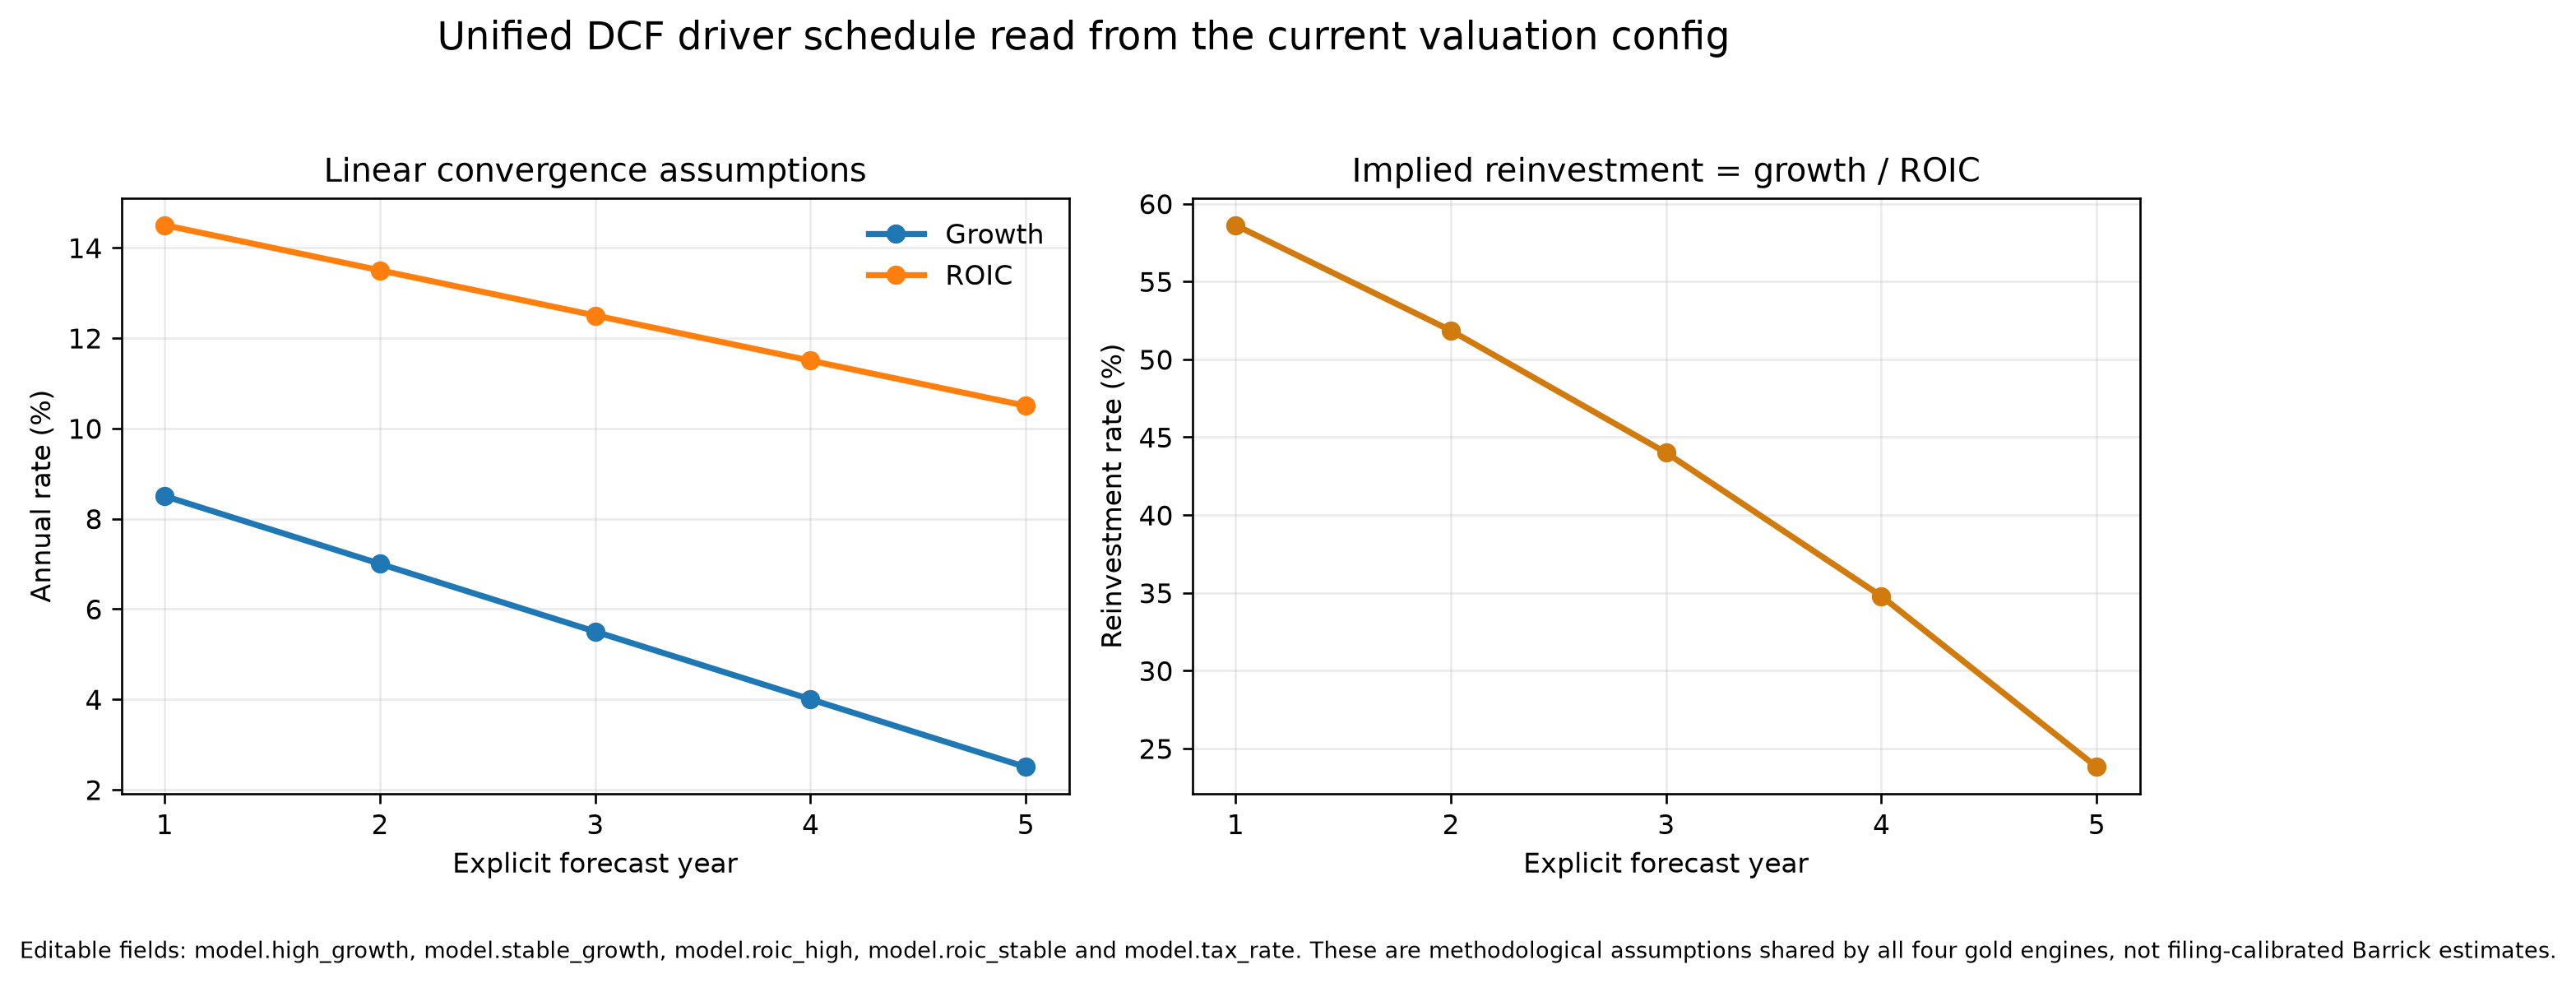
\includegraphics[width=0.98\textwidth]{img/valuation/dcf_driver_schedule.png}
    \caption{Growth, ROIC and implied reinvestment schedule used by the current
    run. These common DCF assumptions do not vary across the four gold-price
    engines.}
    \label{fig:current-dcf-driver-schedule}
  \end{figure}
}{%
  \gapbox{The generated DCF-driver dashboard is unavailable; no editorially
  reconstructed substitute is admitted.}%
}

The annual WACC is not a manually descending list. Starting from \(w_0=9.1\%\),
the code applies
\begin{align}
w_{y+1}&=\bar w+(w_y-\bar w)e^{-\kappa}
       +\sigma_c\varepsilon_{y+1},\\
\sigma_c&=\sigma_w
\sqrt{\frac{1-e^{-2\kappa}}{2\kappa}},
\end{align}
with \(\bar w=8.3\%\), \(\kappa=0.45\), \(\sigma_w=0.9\%\) and independent
standard-normal shocks. The zero-shock path is approximately 8.81\%, 8.63\%,
8.51\%, 8.43\% and 8.38\% for years 1--5. The actual valuation uses 8,192
stochastic WACC paths, created once with seed 20260827 and reused byte-for-byte
under every gold model. Thus the shaded interval in
Figure~\ref{fig:current-wacc-assumption-paths} is discount-rate uncertainty,
whereas differences between model valuation distributions still isolate the
price engine.

\IfFileExists{img/valuation/wacc_assumption_paths.png}{%
  \begin{figure}[H]
    \centering
    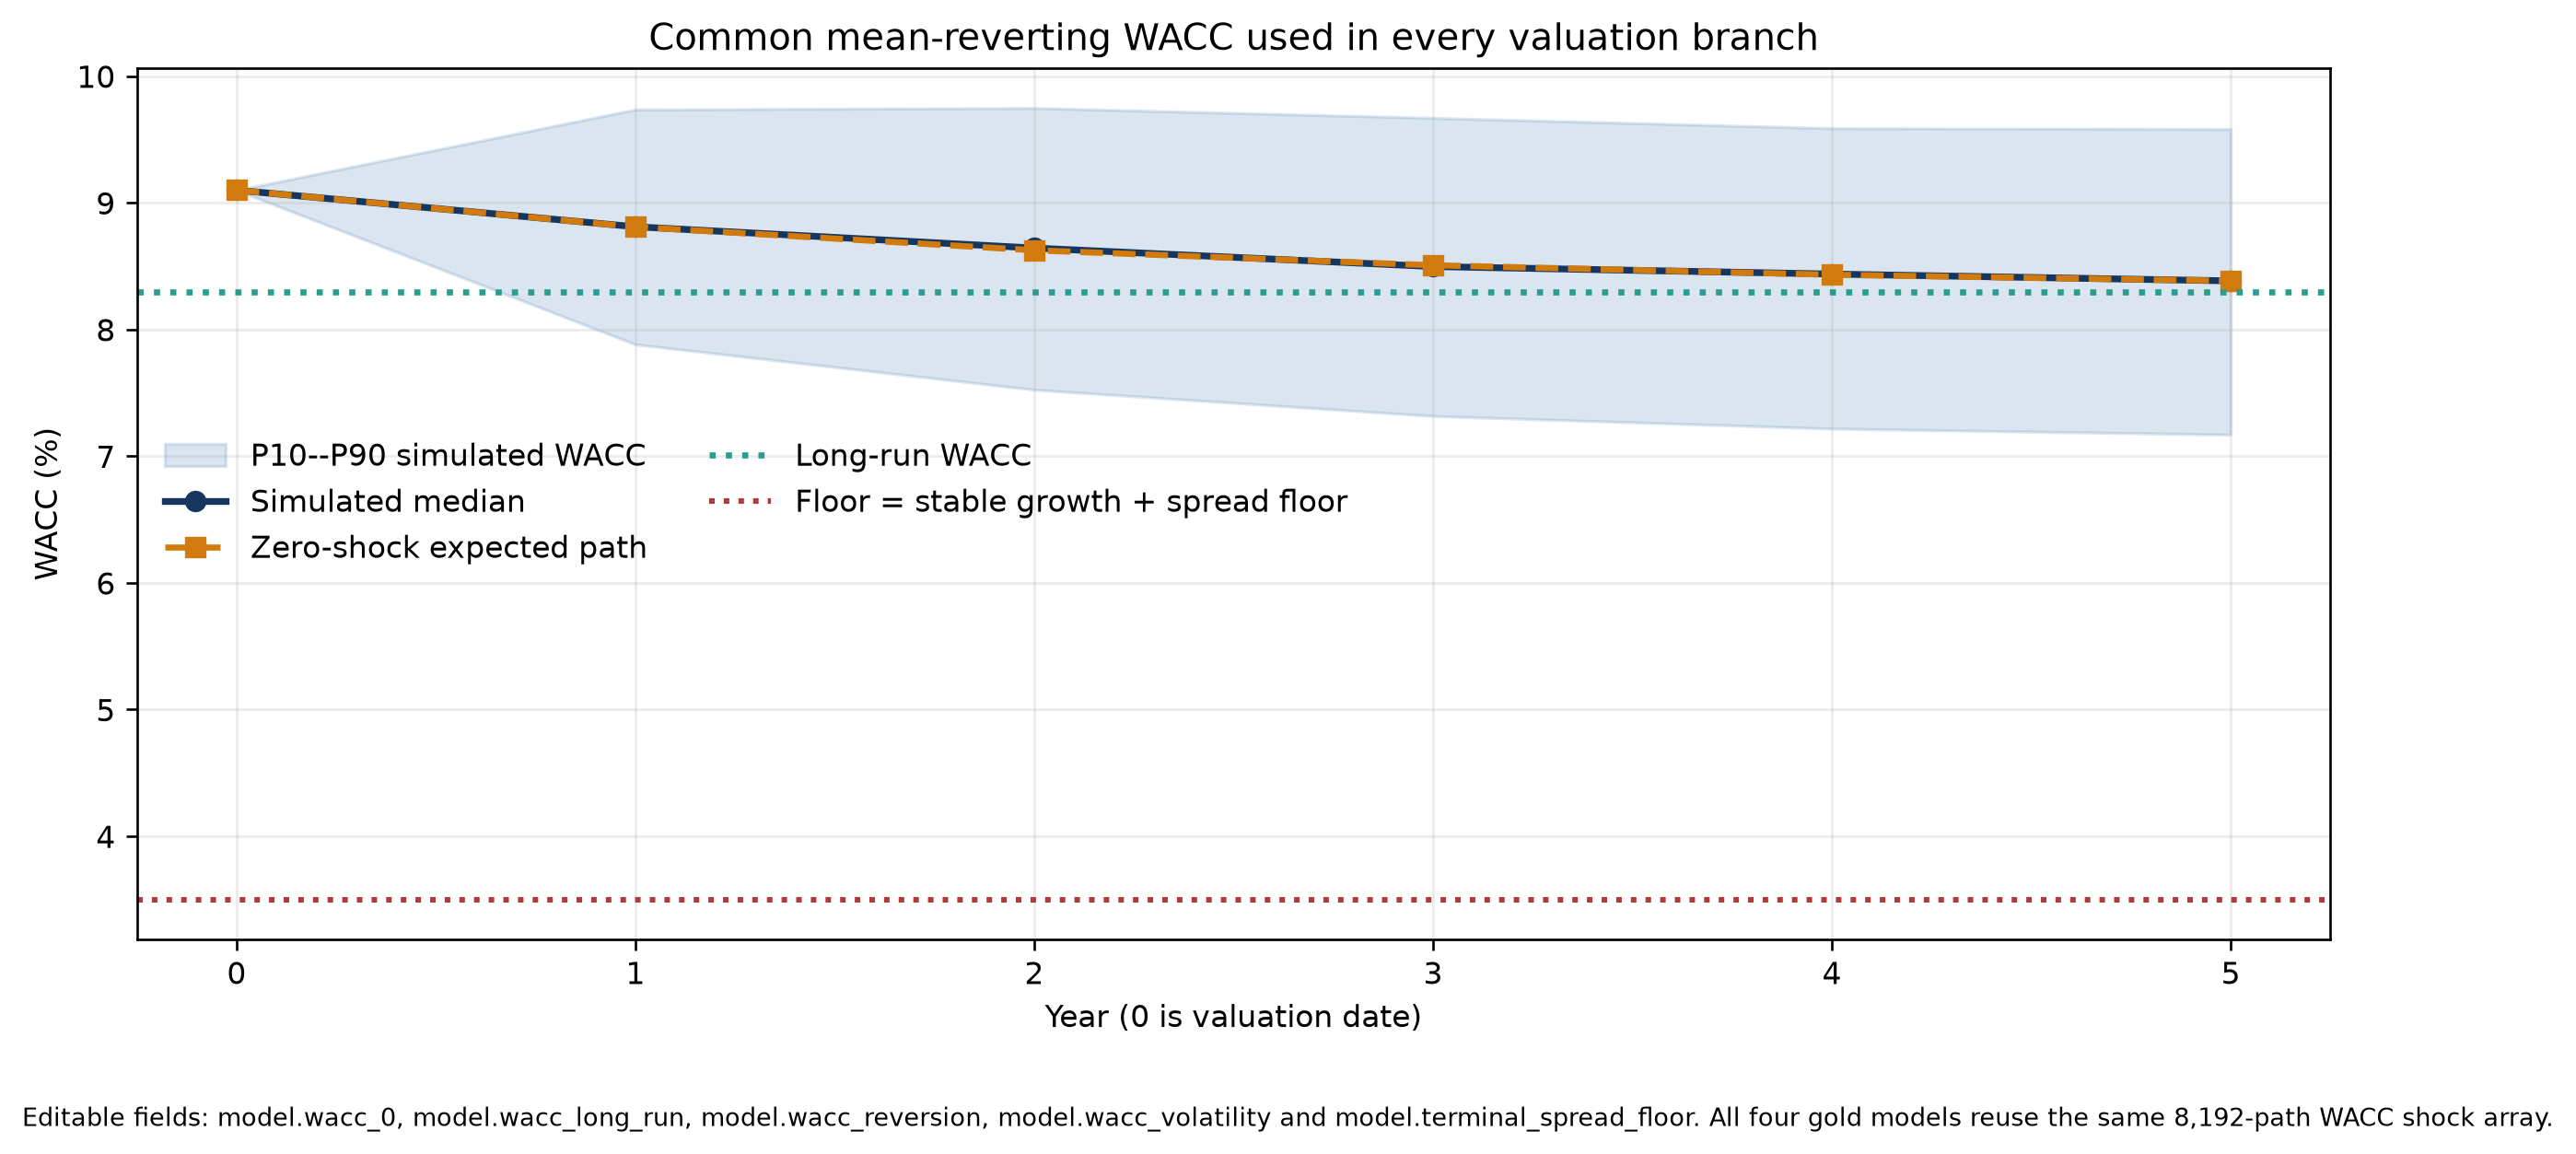
\includegraphics[width=0.95\textwidth]{img/valuation/wacc_assumption_paths.png}
    \caption{Initial WACC, zero-shock mean-reversion path, simulated
    P10--P90 envelope, 8.3\% long-run level and terminal-spread floor used in
    the common valuation layer.}
    \label{fig:current-wacc-assumption-paths}
  \end{figure}
}{%
  \gapbox{The generated WACC-assumption dashboard is unavailable; no
  substitute path is supplied manually.}%
}

The terminal block applies the final positive after-tax component margin,
grows it once, funds stable growth at \(g_s/ROIC_s\), capitalises the resulting
FCFF at \(w_H-g_s\), and then discounts it back over the same path. The left
panel of Figure~\ref{fig:current-terminal-value-mechanics} makes the two most
sensitive editable inputs visible without pretending that the normalized
multiple is a company estimate. The right panel uses the accepted run and
reports how much of positive enterprise value comes from the discounted
terminal block under each price engine. This is the appropriate place to judge
whether the five-year horizon leaves excessive weight in the terminal value.

\IfFileExists{img/valuation/terminal_value_mechanics.png}{%
  \begin{figure}[H]
    \centering
    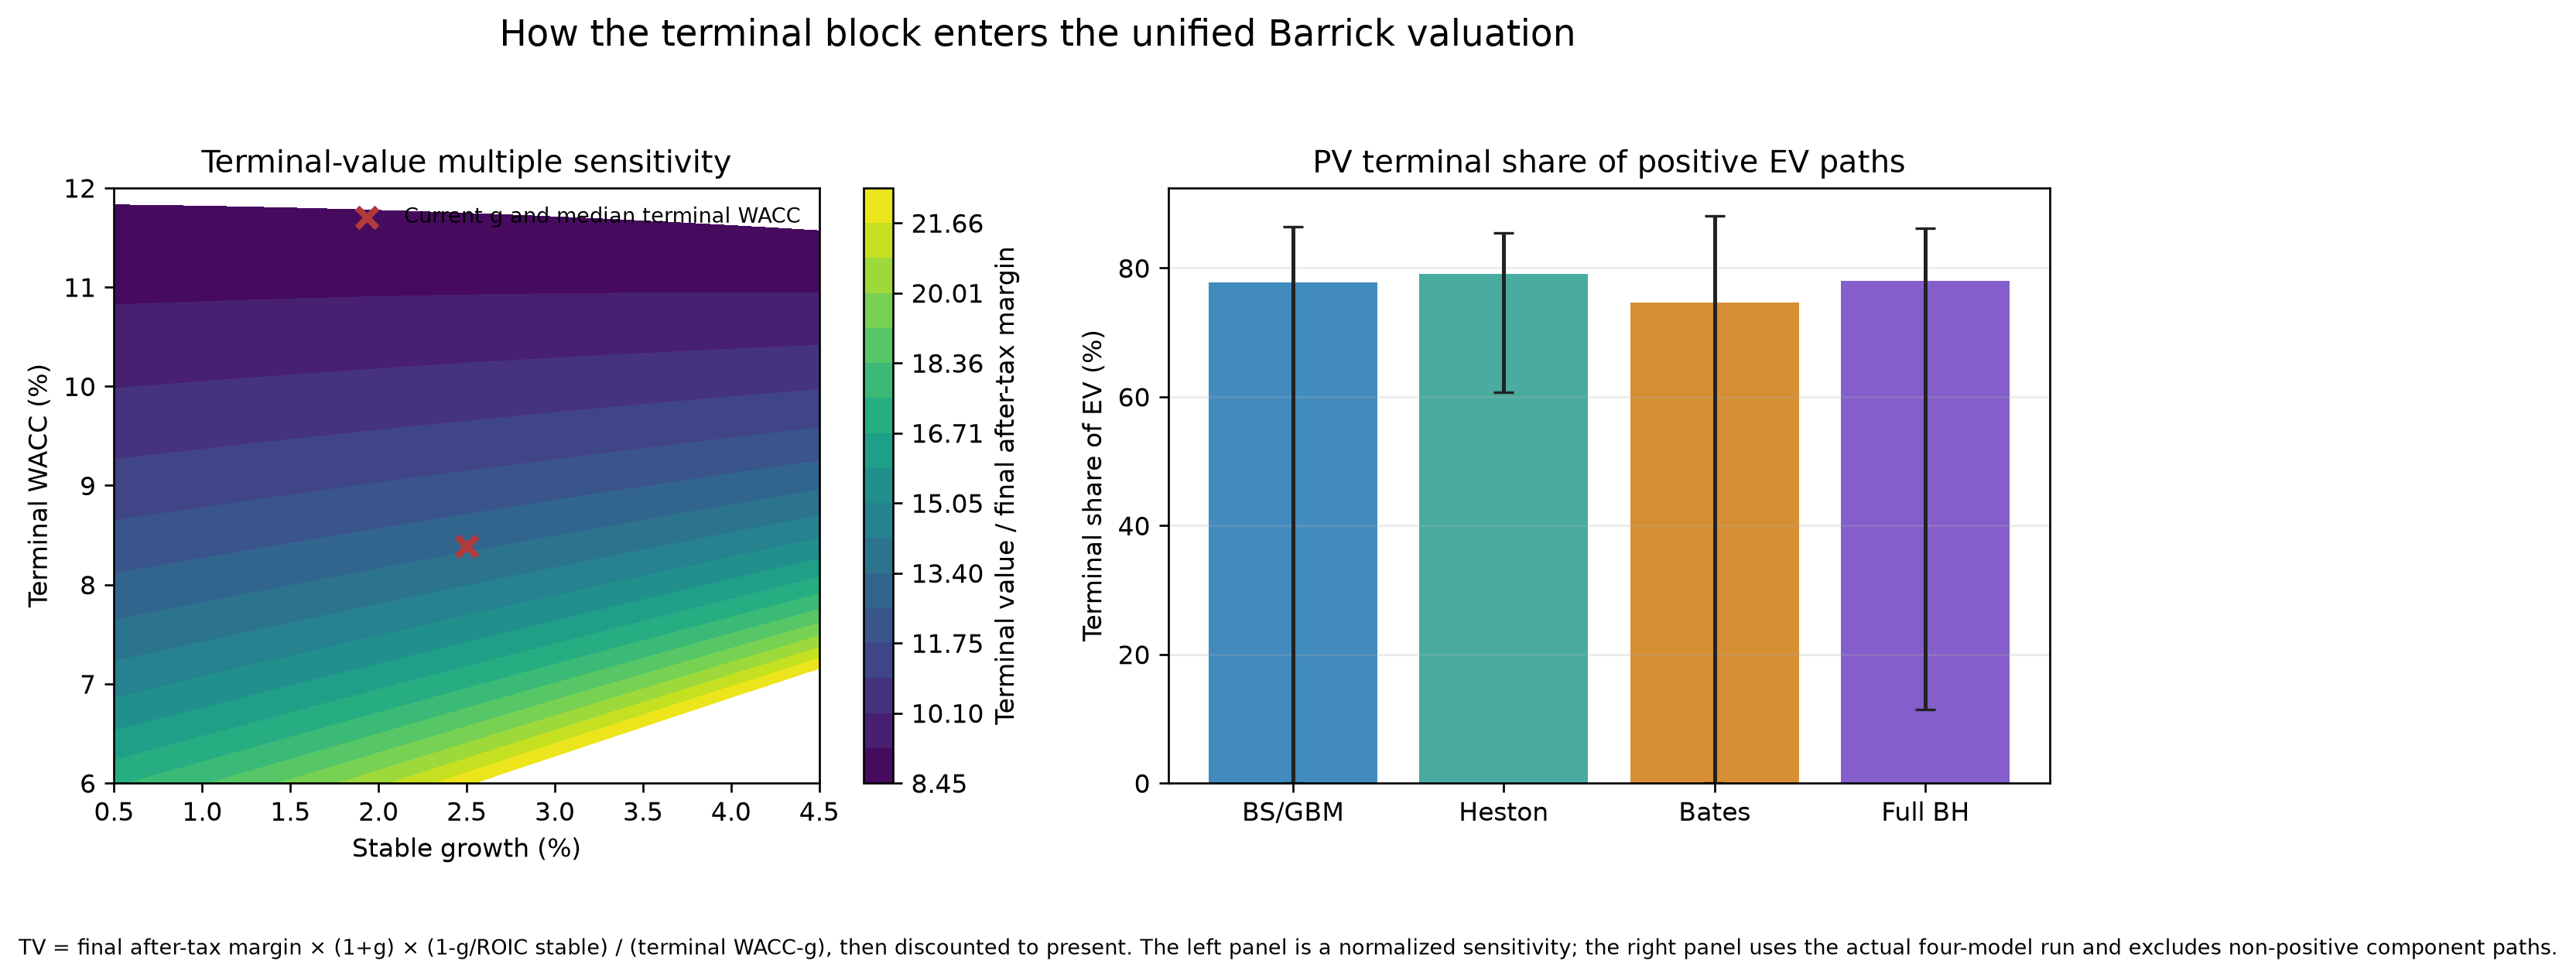
\includegraphics[width=0.99\textwidth]{img/valuation/terminal_value_mechanics.png}
    \caption{Terminal-value mechanics. Left: normalized sensitivity to stable
    growth and terminal WACC at the current stable ROIC. Right: actual-run
    P10, median and P90 terminal contribution to positive enterprise-value
    paths.}
    \label{fig:current-terminal-value-mechanics}
  \end{figure}
}{%
  \gapbox{The generated terminal-value dashboard is unavailable; no manually
  reconstructed sensitivity is admitted.}%
}

This register also clarifies how the project is joined. Team~8 changes only the
gold path; the Barrick/Team~4 operating vector is common; the tax,
growth--ROIC reinvestment rule, WACC array and terminal policy are common; and
the unresolved equity bridge is applied last. Consequently, editing any field
in Table~\ref{tab:current-editable-valuation-parameters} changes all four
branches together. Editing a Team~8 parameter changes only its corresponding
gold-price branch. No Team~4 simulated gold price or demonstrator valuation is
used.

\section{Finite-resource closure for a mining company}

Perpetual growth is not the automatic base case for a miner because reserves,
mine lives and closure obligations are finite. The terminal policy must connect
the explicit asset horizon to depletion, replacement, exploration and future
portfolio renewal. The alternatives in Table~\ref{tab:terminal-closure-alternatives}
are mutually exclusive modelling choices rather than terms to be blended.

\begin{table}[H]
\centering
\caption{Terminal-closure alternatives that must be chosen, not blended.}
\label{tab:terminal-closure-alternatives}
\small
\renewcommand{\arraystretch}{1.12}
\begin{tabularx}{\textwidth}{@{}p{3.00cm}X X@{}}
\toprule
Closure & Required evidence & Main risk \\
\midrule
Finite asset run-off & Mine lives, production decline, closure liabilities and
post-closure cash flows. & Omitting unmodelled replacement or corporate costs. \\
Explicit portfolio renewal & Exploration, development and acquisition
reinvestment tied to additions and future production. & Treating speculative
replacement as certain or costless. \\
Corporate going concern & Sustainable post-horizon FCFF, growth, ROIC, WACC
and continuing asset policy. & Hiding finite-resource economics inside a
perpetual-growth denominator. \\
\bottomrule
\end{tabularx}
\end{table}

\section{From deterministic DCF to a stochastic valuation distribution}

% Sources: Team 5 montecarlo_int, simulation_results and scenarios.
Team 5 extends the three-stage model without changing its accounting logic.
For each draw \(m\), it generates joint paths for operating drivers and WACC,
constructs FCFF, applies pathwise discount factors
\begin{equation}
DF_y^{(m)}=\prod_{s=1}^{y}\frac{1}{1+w_s^{(m)}},
\end{equation}
and returns
\begin{equation}
EV^{(m)}=\sum_{y=1}^{H}FCFF_y^{(m)}DF_y^{(m)}
       +TV_H^{(m)}DF_H^{(m)}.
\end{equation}
The reporting object is the empirical distribution
\(\{EV^{(1)},\ldots,EV^{(M)}\}\), summarised by its median, tail quantiles,
dispersion, terminal-value share and sensitivity measures. Dependence is part
of the model: weak operating states may coincide with higher discount rates,
and growth, margins, ROIC and reinvestment must move as a coherent narrative.

The accepted Team~5 contribution is methodological: distributions, fan
charts, terminal-value shares and driver attribution must be reported, and
Monte Carlo sampling error must be separated from economic dispersion. Its
standalone numerical example uses synthetic value units and is therefore
retained only as a branch-level implementation test. It is intentionally not
shown as Barrick evidence and contributes no simulated company price to the
unified valuation.

The scenario extension similarly varies coherent assumption sets rather than
one cell at a time. In the source illustration, conservative, base and
expansion cases jointly change growth, margin, ROIC, WACC and volatility. The
numerical values remain synthetic, but three methodological controls carry
into the thesis: every scenario must state its joint economic narrative; a
wider absolute distribution can accompany a stronger scenario; and the
terminal-value share must be reported because it can rise as stable economics
improve.

\section{Barrick-specific implementation contract}

The original Team 5 engine is a reproducible synthetic benchmark. It becomes
a Barrick valuation only after every illustrative driver is replaced by a
dated, unit-checked input and the finite-resource closure is selected. The
following table separates completed methodological reuse from open economic
reconciliation.

\begin{table}[H]
\centering
\caption{Team 5 contribution and Barrick-specific admission gate.}
\label{tab:dcf-reuse-gates}
\small
\renewcommand{\arraystretch}{1.12}
\begin{tabularx}{\textwidth}{@{}p{2.7cm}X X@{}}
\toprule
Element & Reusable contribution & Required before a validated Barrick claim \\
\midrule
Accounting perimeter & Operating/non-operating/financing reclassification,
NOPAT and invested-capital logic. & Filing-level mapping for Barrick, with
mining cost, D\&A, capex, tax and closure definitions reconciled. \\
FCFF engine & NOPAT, reinvestment and pathwise discounting identities. & Team
4-to-EBIT bridge, working capital, sustaining/growth capex and dimensional
tests. \\
WACC & Cost-of-equity/debt and capital-weight architecture. & Dated currency-
consistent risk-free curve, ERP, beta, borrowing spread, tax and market-value
weights. \\
Three-stage closure & Joint transition and growth--ROIC--reinvestment
consistency. & Mine horizon and one explicit, tested run-off, renewal or going-
concern policy. \\
Stochastic DCF & Distributional estimator, fan charts, quantiles, terminal
share and sensitivity reporting. & Approved joint scenarios, measure policy,
seeds, convergence and dependence diagnostics. \\
Equity bridge & Enterprise-versus-equity distinction. & Dated net debt, cash,
minorities, streams, other claims, non-operating assets and diluted shares. \\
\bottomrule
\end{tabularx}
\end{table}

The next chapter uses this architecture as a common contract across four gold-
price engines. It reports the conditional Barrick experiment and its validation
in one place; the calibration and predictive evidence itself remains in
Chapter~9 and is not repeated.

\chapter{Unified Barrick Valuation Experiment and Validation}
\chapterstatus{Unified version of the former valuation and validation
chapters. It reports one controlled comparison of four gold-price engines
under a common operating and DCF contract, then evaluates engineering,
numerical, accounting and external validity. Chapter~9 remains the sole home
of option calibration, residual geometry and out-of-sample forecasting, so
those results are referenced rather than repeated here.}

\section{End-to-end experiment contract}

Chapter~11 defined the accounting, discounting and closure rules that must hold
before operating scenarios can become enterprise value, equity value and a
per-share quantity. The integrated experiment is therefore a sequence of typed
transformations rather than one black box:
\begin{align}
\mathcal P_{opt}^{\mathbb Q}
&\longrightarrow
\{S_{t,j}^{GLD,(m)},v_{t,j}^{(m)},N_{t,j}^{J,(m)},
\lambda_{t,j}^{H,(m)}\},\\
&\xrightarrow{\;\mathcal A_{scenario}\;}
\{P_{t,j}^{Au,(m)}\},\\
&\xrightarrow{\;\mathcal A_{operations}\;}
\{Rev_{y,j}^{(m)},\text{component margin}_{y,j}^{(m)}\},\\
&\xrightarrow{\;\mathcal A_{accounting}\;}
\{NOPAT_{y,j}^{(m)},FCFF_{y,j}^{proxy,(m)}\},\\
&\xrightarrow{\;\mathcal A_{DCF}\;}
\{EV_j^{(m)},EqV_j^{(m)},V_{ps,j}^{(m)}\},
\qquad j\in\{BS,H,BP,BH\}.
\end{align}
Each arrow has its own date, unit, measure and validation rule. Team 8 governs
the option-implied gold-price engines already developed and tested in
Chapter~9; Team~4 supplies the operating methodology and forecasts, refreshed
with Barrick actuals for 2026Q1--Q2; the unified DCF governs cash-flow
construction, discounting and the equity bridge; Team~3 supplies simulation
diagnostics. No source article alone authorises the last arrow.

\begin{table}[H]
\centering
\caption{Interfaces and stop conditions in the unified experiment.}
\label{tab:unified-interface-contract}
\scriptsize
\setlength{\tabcolsep}{3pt}
\renewcommand{\arraystretch}{1.10}
\begin{tabularx}{\textwidth}{@{}p{2.15cm}p{2.15cm}X X@{}}
\toprule
Stage & Source authority & Required contract & Stop condition \\
\midrule
Option scenarios & Teams 8 and 6 & Versioned snapshot, rate dates, parameter
objects, \(\mathbb Q\), time grid and seed. & A calibration or predictive
claim is inconsistent with Chapter~9. \\
Gold bridge & Team 8; unified adapter & Conditional transfer of
GLD/\(\mathbb Q\) distributional shape to gold USD/oz from one starting
level. & A GLD-level conversion, physical forecast or \(\mathbb Q\)-to-
\(\mathbb P\) transformation is implied rather than declared. \\
Operations & Team 4 & Production and cost units, ownership, frequency,
dependence and accounting definition. & CoS/AISC/D\&A/capex treatment or input
perimeter is ambiguous. \\
FCFF and closure & Team 5 & Taxes, reinvestment, WACC, horizon and terminal
policy. & Accounting identities, \(w>g\) or finite-resource closure fail. \\
Equity and per share & Team 5 plus corporate inputs & Net debt, minorities,
other claims, non-operating assets, diluted shares and matching listing. &
Bridge items do not reconcile to one dated filing and security. \\
Reporting & Teams 3 and 5; unified pipeline & Replay, quantiles, sensitivity
and hash-linked CSV/JSON/figure bundle. & A table and figure do not derive from
the same accepted run. \\
\bottomrule
\end{tabularx}
\end{table}

\section{Controlled design: one changing layer}

The experiment isolates the price-engine effect. It evaluates the four Team 8
engines named in Chapter~9 while holding production, unit costs, taxes, WACC,
terminal policy and equity inputs constant. Their stochastic laws and fit
diagnostics are not restated here. The relevant experimental fact is simpler:
only the gold-price scenario generator changes across the four branches.

The 20-quarter operating contract uses Barrick actual production and Cost of
Sales in 2026Q1--Q2, followed by Team~4 forecasts from 2026Q3. The actual and
forecast segments are labelled separately rather than presented as one
homogeneous source. Tax, growth, ROIC, stochastic WACC, terminal-growth and
equity-bridge inputs are common, and the same WACC shock array is reused in all
branches. Consequently, differences among the four output distributions can
be attributed to the gold-price engine within this common contract. They
cannot be attributed to mine plans, extraction uncertainty or cost inflation,
because those layers do not vary.

The exact editable values, their annual paths and their terminal-value effect
are disclosed once in Section~\ref{sec:executable-valuation-assumptions}, with
generated CSV/JSON sidecars. They are not repeated here: this chapter uses the
dashboard as the common downstream contract and focuses only on what changes
when the Chapter~9 gold engine changes.

The earlier Team~4 NSS, IV, GBM and stochastic EBITDA chain was a standalone
demonstrator. It is not imported into this experiment. Team~4 contributes only
the operating decomposition and forecast continuation; Team~8 alone generates
the current price paths. The current LSE NSS term structure is a separate,
newly fitted Team~8/unified input and is therefore retained.

\section{Measure, dates and simulation design}

Option calibration identifies a risk-neutral law useful for market-implied
scenario analysis. It does not identify physical drift or a causal forecast of
realised gold. The adapter is therefore labelled a \emph{conditional transfer
of GLD/\(\mathbb Q\) distributional shape to gold USD/oz}. Each engine
restarts at USD~4,417/oz, Barrick's Q2 2026 average realised price used only
as a common level anchor. The procedure neither
converts GLD share levels into physical gold nor estimates a
\(\mathbb Q\)-to-\(\mathbb P\) map.

The date vector remains visible: the anchor quarter ends 30 June 2026, the
Treasury curve is dated 24 July, while the Barrick close and current Team~8
surface are dated 27 August. The current surface is used for recalibration. The
remaining asynchrony restricts
the output to a conditional model comparison.

The numerical design uses 8,192 paths, 260 fine steps and 13 fine steps per
quarter over 20 quarters. All price engines use base seed 20260827; WACC uses
seed 20260827 and is generated once. The model-specific stream construction is
documented in Chapter~9. At the corporate layer, the important control is that
the same accepted operating arrays and WACC paths enter all branches.

\section{Executable method and result bundle}

% Generated fragments are admitted only from the authoritative final pointer.
\IfFileExists{chapters/generated/current-valuation-method.tex}{%
  \paragraph{Current conditional multi-model adapter.}

The controlled experiment varies only the gold-price engine. Black--Scholes/
GBM, Heston, Bates--Poisson and Full Bates--Hawkes use the Team~8 parameters
recalibrated to the 2 September 2026 GLD surface. All engines start from the same
USD~4,417/oz level anchor, defined as Barrick's Q2 2026 average realised gold
price. It is neither a point-in-time spot observation nor a Team~4 simulated
price. Fourteen U.S. Treasury observations from 2 September 2026 are fitted
with the same-date Nelson--Siegel--Svensson curve (RMSE 2.0608 basis points
against the continuous par-yield proxy). Option calibration uses the fitted
rate at each maturity; quarterly paths use integral-preserving forward rates.
This is not a bootstrapped zero curve. The conditional bridge transfers option-implied shape under
$\mathbb Q$; it does not establish a one-for-one GLD conversion or a validated
$\mathbb Q$-to-$\mathbb P$ transformation.

This current NSS is independent of the legacy Team~4 demonstrator. The
operating contract is separate. Barrick's reported production and Cost of
Sales replace the first two quarters of 2026; the Team~4 production and cost
forecasts begin at 2026Q3. The legacy Team~4 NSS fit, implied-volatility inversion,
GBM paths and illustrative stochastic EBITDA valuation are explicitly
excluded. For model $j$, quarter $t$ and path $m$, the adapter forms
\begin{equation}
M_{t,j}^{(m)}=\frac{\bigl(P_{t,j}^{Au,(m)}-C_t\bigr)Q_t}{1000},
\end{equation}
where $Q_t$ is in thousand troy ounces and $C_t$ is in USD/oz. One common DCF,
WACC stream and equity bridge then maps every price branch to per-share value.

The run uses 8,192 paths, 260 fine steps aggregated to 20 quarters, aligned
price-engine seed 20260902 and independent WACC seed 20260902. The WACC shock
array is generated once and reused byte-identically. Therefore cross-model
differences arise from the Team~8 price law, while the actual/forecast
operating boundary and all corporate assumptions remain common.
%
}{%
  \gapbox{The accepted multi-model method fragment is unavailable. No
  substitute method claim is supplied editorially.}%
}

For \(M\) admitted paths from model \(j\), the empirical per-share
distribution and quantiles are
\begin{equation}
\widehat F_j(x)=\frac{1}{M}\sum_{m=1}^{M}
\mathbf 1\!\left\{V_{ps,j}^{(m)}\leq x\right\},
\qquad
\widehat Q_{u,j}=\inf\{x:\widehat F_j(x)\geq u\}.
\end{equation}
The table and figure below derive from the same versioned result bundle.

\IfFileExists{chapters/generated/current-valuation-multimodel-quantiles.tex}{%
  \begin{table}[H]
\centering
\caption{Barrick conditional value-per-share quantiles by gold-price model.}
\label{tab:conditional-multimodel-valuation-quantiles}
\setlength{\tabcolsep}{8pt}
\resizebox{\textwidth}{!}{%
\begin{tabular}{@{}r r r@{\hspace{10pt}}r r@{}}
\toprule
\textbf{Quantile} & \textbf{BS/GBM} & \textbf{Heston} &
\textbf{Bates--Poisson} & \textbf{Full Bates--Hawkes} \\
\midrule
P01 & -0.34 & -0.89 & -0.74 & -1.05 \\
P05 & 1.67 & 1.35 & 1.51 & 1.33 \\
P10 & 3.71 & 3.27 & 3.58 & 3.13 \\
P25 & 15.74 & 15.47 & 15.89 & 14.85 \\
P50 & 35.87 & 35.67 & 35.84 & 35.14 \\
P75 & 64.52 & 64.87 & 64.79 & 65.24 \\
P90 & 103.48 & 103.63 & 101.43 & 104.72 \\
P95 & 132.60 & 137.34 & 131.45 & 134.36 \\
P99 & 213.80 & 218.36 & 199.56 & 216.26 \\
\bottomrule
\end{tabular}%
}
\par\smallskip
\footnotesize Values are USD/share; the observed \texttt{B} close is USD~44.13
on 2 September 2026. Operations use Barrick 2026Q1--Q2 actuals and Team~4
forecasts from 2026Q3; the Team~4 price demonstrator is excluded. Negative
lower-tail proxies reflect the unreconciled research DCF and are not target
prices, confidence intervals or recommendations.
\end{table}
%
}{%
  \gapbox{The four-model quantile table is unavailable. No values are supplied
  editorially.}%
}

\IfFileExists{img/valuation/multimodel_value_distribution_comparison.png}{%
  \begin{figure}[H]
    \centering
    
\includegraphics[width=0.98\textwidth]{img/valuation/multimodel_value_distribution_comparison.png}
    \caption{Kernel-density comparison of conditional Barrick value per share
    under the four Chapter~9 gold-price engines. Production, unit cost, DCF,
    WACC and equity inputs are common; the vertical line is the USD 47.27
    completed \texttt{B} close on 27 August 2026.}
    \label{fig:multimodel-value-distribution-comparison}
  \end{figure}
}{%
  \gapbox{The accepted four-model density comparison is unavailable until it
  is copied from the authoritative result manifest.}%
}

The medians are USD~34.50 for Black--Scholes/GBM, USD~39.48 for Heston,
USD~23.99 for Bates--Poisson and USD~34.94 for Full Bates--Hawkes. Relative
to the USD~47.27 close, the differences are USD~12.77, 7.79, 23.28 and
12.33, respectively. The close lies between the 59.94th and 66.11th model
percentiles, and the simulated frequencies \(P(V_{ps}>47.27)\) range from
33.89\% to 40.06\%. Thus every branch places
the observed close above its conditional median, but well inside a broad
distribution. This is not proof that the market is mispriced.

Model choice is more visible in the tails. P10 spans USD~0.37--10.02 and P90
USD~91.37--137.65. Full Bates--Hawkes has P01 USD~-0.54 and P99 USD~218.11;
Heston has the highest P01, USD~1.01, and the lowest P99, USD~165.19. Holding
operations and DCF fixed therefore compresses median differences while
preserving economically meaningful tail differences.

\section{Layered validation}

Validation is not one score. Source parity, implementation tests, current-data
integrity, calibration, prediction, simulation stability and corporate
reconciliation answer different questions. The option-specific calibration
and chronological evidence is evaluated in Chapter~9. This section tests the
new information created by integration.

\IfFileExists{chapters/generated/current-valuation-diagnostics.tex}{%
  \paragraph{Run diagnostics and falsification gates.}

The current evidence bundle uses the 2 September Team 8 snapshot and one
versioned four-model valuation. The refresh-specific regression suite verifies
the current input contract, separates the Heston in-sample ranking from the
Full Bates--Hawkes OOS ranking, and tests the path adapter. The operating
arrays, unified DCF assumptions and single WACC shock array have identical
hashes in all four branches. Empirical quantiles are ordered, and EV-to-equity
and equity-to-per-share mappings remain explicit.

These software gates do not validate the GLD-to-gold basis, a physical-measure
forecast, corporate accounting, zero equity-bridge placeholders or the share
proxy. The current calibration contains 605 eligible calls and 64 retained
contracts, with 14 same-date Treasury tenors. Historical suite counts and
47-image audits belong to the August bundle and do not certify newly refreshed
figures without a new provenance check.
%
}{%
  \gapbox{The accepted diagnostic fragment is unavailable. No output may be
  promoted without deterministic replay, identity tests and manifest checks.}%
}

\begin{table}[H]
\centering
\caption{Evidence hierarchy for the integrated valuation.}
\label{tab:validation-evidence-hierarchy}
\scriptsize
\setlength{\tabcolsep}{3pt}
\renewcommand{\arraystretch}{1.10}
\begin{tabularx}{\textwidth}{@{}p{2.20cm}X X X@{}}
\toprule
Layer & Accepted evidence & Still open & Allowed conclusion \\
\midrule
Source integrity & Frozen hashes and admitted parity outputs for the eight
team modules. & Historical runtimes, licences and excluded assets recorded in
their source audits. & The admitted files are stable inputs, not independently
re-estimated facts. \\
Implementation & Team 8 and LSE boundary tests; unified complete and focused
suites; legacy/refactor equality in one runtime. & Full independent formula
review and all historical-market replay. & The tested contracts are
implemented within their declared tolerance. \\
Experiment identity & Same separated operating contract, unified DCF inputs and WACC paths in
all branches; monotone quantiles and pathwise bridge identities. & Stochastic
production/cost propagation and filing reconciliation. & Differences among
branches isolate price-engine sensitivity under the common contract. \\
Accounting & FCFF, discounting and per-share identities are executable. &
Actual debt, cash, minorities, other claims, share count and finite-mine
closure. & Outputs are conditional proxies rather than validated fair values. \\
External validity & Dates, units and \(\mathbb Q\)-scenario semantics are
serialized. & GLD-to-gold basis, \(\mathbb Q\)-to-\(\mathbb P\) bridge and
synchronous inputs. & The experiment is reproducible but not a physical gold
forecast. \\
\bottomrule
\end{tabularx}
\end{table}

\section{Numerical and simulation robustness}

The numerical gate covers analytical-pricer limits upstream, path-
discretisation bias, path-count convergence, seed stability, finite outputs,
quarterly aggregation and pathwise accounting identities. Monte Carlo error
and economic dispersion are distinct: the first concerns whether the numerical
estimator has converged; the second is the spread induced by the assumed
stochastic and corporate inputs.

The accepted branch passed the complete 57-test suite, while the autonomous
figure audit passed all 47 analytical images. Quantile sequences are ordered; every
path satisfies enterprise-to-equity and equity-to-per-share identities; and
directional tests confirm that higher gold raises the proxy value while higher
costs or discount rates lower it. Historical Sobol array hashes that vary with
the resolved runtime are retained as a reproducibility finding rather than
mislabelled as an economic change.

These gates make the four distributions comparable computational outputs.
They do not validate the economic adapters through which GLD option scenarios
become gold revenue and then Barrick equity.

\section{Accounting and economic validation}

The current experiment keeps one operating vector deterministic after the
explicit actual/forecast handoff. That design supports attribution but
suppresses production and cost uncertainty. The unified DCF is likewise a common research contract, not a
filing-reconciled model. Debt, cash, minority interests, non-operating assets
and other claims remain zero placeholders, while 1,675.51 million diluted
shares are not reconciled to a common filing date. Equality of enterprise and
equity value in the run is therefore an input consequence, not a conclusion
about Barrick's balance sheet.

Economic validation must additionally reconcile revenue to volumes and
realised prices; operating margin to EBIT; NOPAT, reinvestment and FCFF by path
and year; positive discount factors; admissible terminal denominators; and the
EV-to-equity adjustments described in Chapter~11. Sensitivities must use native
units and follow directions implied by the equations. No option-pricing fit can
substitute for these controls.

\section{External validity and information limits}

GLD option values, the GLD share price, physical gold in USD/oz, Barrick's
realised selling price and mine-level cash flow are distinct objects. The run
transfers the shape of a GLD/\(\mathbb Q\) distribution to paths restarted at
the USD~4,417/oz Barrick realised-price anchor without a validated
physical-measure map. The
asynchronous dates listed above remain a limitation after every software test
passes.

The information set also excludes timestamped macroeconomic and geopolitical
news. Such events may enter indirectly through prices, implied volatility and
jumps, but the current filtration cannot identify their causal contribution.
An NLP or machine-learning extension is therefore a genuine future research
question requiring leakage controls and chronological evaluation, not an
unfinished step of the present valuation.

\section{What the integrated experiment establishes}

The combined result is intentionally bounded. The project has completed the
planned integration of the Team~8 price layer, separated Team~4/Barrick
operating layer and unified stochastic DCF contract. Under one common set of operating and corporate
assumptions, all four price engines place the USD 47.27 close above their
conditional medians while retaining substantial probability mass above it.
The close remains inside every broad distribution, so the common direction is
a scenario result rather than evidence of mispricing.

The experiment also identifies where model form matters: price-engine choice
changes tail geometry more than the median under this common downstream
contract. What remains open is not the act of integration itself, but the
economic validation of its commodity, measure, operating, accounting and
terminal-closure interfaces. The unnumbered conclusion that follows separates
those limitations from the next genuinely new research programme.

\chapter*{Conclusion and Future Research}
\addcontentsline{toc}{chapter}{Conclusion and Future Research}
\markboth{Conclusion and Future Research}{Conclusion and Future Research}
\chapterstatus{Unnumbered synthesis of findings, present limitations and
genuinely new research directions. Items already completed by the unified
project are recorded as results rather than repeated as future work.}

\section*{What the project has completed}

This thesis converts eight specialised studies into one traceable research
architecture. Its main contribution is the separation and subsequent
connection of five objects: the historical gold series, the option-implied
gold-price law, production, unit cost and corporate cash flow. The resulting
chain is explicit enough to identify which evidence supports each output and
where a change of data, units, measure or accounting perimeter occurs.

Several tasks described as future work in the standalone articles are now
complete. The Team 8 project no longer stops at Black--Scholes, Heston or
independent Bates jumps: it contains the full affine Bates--Hawkes
specification, constrained calibration, residual and smile diagnostics,
four-model path simulation and a dense-only rolling comparison over 30 origins and 4,667 common forecasts. Its
price scenarios have also been connected to Barrick 2026Q1--Q2 actuals, the
Team~4 forecast from 2026Q3 and the unified DCF/WACC/equity contract. The
Team~4 price demonstrator is excluded. The valuation is therefore an implemented
four-branch experiment, not a proposed future integration.

Under that common contract, the four conditional Barrick medians lie between
USD~35.14 and USD~35.87 per share, below the completed USD~44.13 close
on 2 September 2026. The close remains inside every broad distribution,
with 40.76--41.92\% of simulated values above it. Full Bates--Hawkes is the
primary OOS-ranked structural scenario and gives a median of USD~35.14,
whereas Heston is the current-snapshot fit winner. The shared direction
is a property of the admitted assumptions, not evidence of market mispricing.

The comparison further shows that changing the gold-price law affects the
tails more than the central corporate value when production, cost, WACC and
the equity bridge are fixed. This is a useful attribution result: it identifies
where price-model complexity propagates through the DCF and where downstream
assumptions compress or dominate its effect.

\section*{Present limitations}

The completed integration remains conditional at several economic interfaces.
First, GLD option dynamics are estimated under \(\mathbb Q\), whereas a
long-horizon operating valuation would ideally use scenarios justified under
\(\mathbb P\). Restarting the option-implied engines at a physical-gold level
transfers distributional shape; it is not a validated GLD-to-gold conversion
or change of measure. The gold start, Treasury curve, calibration surface,
Barrick close and current surface audit are explicitly dated: the market snapshot is 2 September, while the realised-price anchor is a Q2 average.

Second, the unified run uses Barrick actuals only for 2026Q1--Q2 and fixes the
Team~4 forecast thereafter. That design isolates price-engine risk but does not propagate reserve,
grade, recovery, energy, labour, mine-mix or closure uncertainty. Dependence
between gold prices and operating conditions is therefore not estimated.

Third, Team 5 supplies a coherent DCF architecture rather than a
filing-reconciled Barrick model. The operating-to-EBIT bridge, cash taxes,
working capital, sustaining and growth capex, debt, cash, minorities, streams,
other claims, non-operating assets and diluted shares require one dated
corporate reconciliation. The present zero bridge items and share-count proxy
are assumptions. Finite-mine closure also remains less developed than the
generic going-concern terminal block.

Finally, a sophisticated stochastic law does not eliminate model risk. The
current cross-section favours Heston, whereas Full Bates--Hawkes leads the rolling OOS ranking. Its branching ratio is 0.5569, not the former August floor. No model beats interpolated IV persistence. Parameter pressure,
surface sampling, optimizer dependence, regime shifts and the choice of
physical-measure transformation remain sources of uncertainty.

Costs retain a persistent trend without additional technology-driven reductions.
This is prudential relative to otherwise identical efficiency-improvement
scenarios, not a mathematical lower bound. Stochastic operating costs would
introduce favourable and adverse outcomes, and their conditional mean could
remain smooth. Productivity improvements and their investment costs must be
evaluated jointly with the growth already included in the DCF.

\section*{Future research programme}

The next research cycle should begin with economic reconciliation rather than
another layer of stochastic complexity. A dated Barrick data contract should
map mine-level production, realised prices, royalties, cash costs, AISC,
depreciation, sustaining and growth capex, working capital, taxes and closure
liabilities into EBIT, invested capital and FCFF. Debt, cash, minority
interests, streams, non-operating assets and diluted shares should then close
the EV-to-equity bridge to the same filing and listing.

The commodity interface requires a separate empirical programme. The GLD-to-
physical-gold basis should be estimated and stress-tested, and risk-neutral
option scenarios should be converted into physical scenarios through an
explicitly validated risk-premium or filtering model. Only after that step can
the long-horizon paths be interpreted as more than option-implied conditional
shapes.

Operating uncertainty should then be reintroduced jointly. Team 4 production
and cost models can be sampled alongside price, but their dependence structure
must be estimated or scenario-defined. Mine depletion, expansion projects,
reserve conversion, inflation, energy and foreign-exchange shocks should feed
an explicit finite-resource closure. The comparison can then be repeated to
measure whether gold-model choice or operating/accounting uncertainty explains
more of the equity-value distribution.

A later information layer may augment the filtration with timestamped
macroeconomic and geopolitical data. News embeddings, NLP classifications or
machine-learning forecasts are admissible only with event-time alignment,
leakage controls, pre-declared benchmarks and true chronological evaluation.
The relevant question is not whether a flexible model improves in-sample fit,
but whether incremental information improves forecasts beyond price,
volatility and persistence benchmarks.

Further model research may examine time-varying risk premia, regime-dependent
parameters, model averaging and a rough-Hawkes option-pricing construction.
Those extensions should be judged through the same hierarchy used here:
mathematical admissibility, deterministic implementation tests, dated
out-of-sample evidence and economic propagation through a reconciled corporate
model.

\section*{Concluding synthesis}

The project demonstrates the value of interdisciplinarity in applied finance.
Probability, stochastic calculus, econometrics, numerical methods,
optimization, accounting and corporate valuation are not parallel subjects in
this setting; each constrains a different interface of the same experiment.
The strongest outcome is therefore not one point estimate or one preferred
model. It is a reproducible framework that keeps historical evidence,
option-implied information, operating assumptions and accounting claims
separate until the moment they are deliberately connected.

Within that framework, Full Bates--Hawkes offers the richest admitted
description of current option-implied variance and clustered jumps, while the
four-model valuation shows how little a better surface fit alone can establish
about a mining company's equity. The thesis closes with a conditional result,
an explicit inventory of unresolved economic bridges and a research programme
capable of testing them. It does not issue a fair-value certification, target
price or investment recommendation.


\begin{references}
\bibitem{team1}
Stefano Falcione and Marco Fracca, \emph{Black--Scholes Foundations}, Barrick project source article, supplied workspace copy.

\bibitem{team2}
Filippo Triassi and Giorgio Zoccatelli, \emph{OLS and Dynamic Correlations}, Barrick project source article, supplied workspace copy.

\bibitem{team3}
Andrea Rostagno and Francesco Florio, \emph{Monte Carlo Risk}, Barrick project source article, supplied workspace copy.

\bibitem{team4}
Giacomo Scali and Jacopo Foralosso, \emph{Component-Driven EBITDA}, Barrick project source article, supplied workspace copy.

\bibitem{team5}
Federico Vesco, Lorenzo Pietra and Bader Moussaif, \emph{Three-Stage DCF}, Barrick project source article, supplied workspace copy.

\bibitem{team6}
Davide Sisto and Matteo Armando, \emph{Beyond Black--Scholes}, Barrick project source article, supplied workspace copy.

\bibitem{team7}
Davide D'Amico and Pietro Weisz, \emph{Gold Volatility Dynamics}, Barrick project source article, supplied workspace copy.

\bibitem{team8}
Salvatore Gabriele Messina and Alessandro Coco, \emph{Gold Options Stochastic Modeling}, Barrick project source article, supplied workspace copy.

\bibitem{lse-2026}
London Strategic Edge, \emph{Market-data and options datasets}, provider snapshot accessed 28 August 2026. Aggregate statistics and derived figures are reported under the project's non-redistribution boundary.

\bibitem{barrick-name-2025}
Barrick Mining Corporation, \emph{Barrick Announces Name Change to Barrick Mining Corporation and Election of Directors}, 6 May 2025, \href{https://www.barrick.com/English/news/news-details/2025/barrick-announces-name-change-to-barrick-mining-corporation-and-election-of-directors/default.aspx}{official corporate release}.

\bibitem{barrick-about-2026}
Barrick Mining Corporation, \emph{About Barrick}, corporate profile accessed 27 August 2026, \href{https://www.barrick.com/English/about/default.aspx}{official company profile}.

\bibitem{imf-war-inflation-2022}
International Monetary Fund, \emph{War Dims Global Economic Outlook as Inflation Accelerates}, 19 April 2022, \href{https://www.imf.org/en/Blogs/Articles/2022/04/19/blog-weo-war-dims-global-economic-outlook-as-inflation-accelerates}{IMF analysis}.

\bibitem{ecb-gold-risk-2025}
European Central Bank, \emph{Gold demand: the role of the official sector and geopolitics}, Financial Stability Review, May 2025, \href{https://www.ecb.europa.eu/press/financial-stability-publications/fsr/focus/2025/html/ecb.fsrbox202505_02~7f616fcd3f.en.html}{ECB analysis}.

\bibitem{fed-gold-reserves-2025}
Board of Governors of the Federal Reserve System, \emph{Exploring Central Bank Gold Purchases and the Dollar's Role in International Reserves}, International Finance Discussion Papers, \href{https://www.federalreserve.gov/econres/ifdp/exploring-central-bank-gold-purchases-and-the-dollars-role-in-international-reserves.htm}{Federal Reserve paper}.

\bibitem{wgc-gdt-q2-2026}
World Gold Council, \emph{Gold Demand Trends Q2 2026: Central Banks}, accessed 27 August 2026, \href{https://www.gold.org/goldhub/research/gold-demand-trends/gold-demand-trends-q2-2026/central-banks}{demand report}.

\bibitem{github-placeholder}
Barrick Gold Research Teams, \emph{Stochastic Valuation of Barrick Mining: unified thesis and supporting code}, Starting Finance Club PoliTo, \href{https://github.com/StartingFinanceClubPoliTo/Research/tree/main/Barrick-Gold/Barrick\%20Mining\%20UNIFICATO}{Barrick Mining UNIFICATO repository}, accessed 29 August 2026.
\end{references}

\end{document}
